\documentclass[justified,a4paper,symmetric,nobib,notoc]{tufte-book}

% Packages setup
\usepackage[brazil,safe=bib]{babel}
\usepackage{hyphenat}
\usepackage[backend=biber, style = authoryear]{biblatex}
\renewcommand{\cite}[2][0pt]{\sidenote[][#1]{\fullcite{#2}}} % citations as sidenotes

%\usepackage{bookmark} % Dá problema com o tamanho da fonte dos captions
%\hypersetup{hidelinks=true,unicode}

\usepackage[T1]{fontenc} 
\usepackage[utf8]{inputenc}						% Pacotes pra escrever
\usepackage[brazil]{babel}						% em português
%\usepackage[fixlanguage]{babelbib}
%\usepackage{biblatex}
\usepackage[np]{numprint}
\usepackage{mathcomp}
\usepackage{amsmath}
\usepackage{amssymb}
\usepackage{lipsum}
\usepackage{tikz}
\usepackage{tikz-3dplot}
\usepackage{gnuplot-lua-tikz}
\usepackage{mathtools}
%\usepackage[small, sc]{caption}
\let\tuftemarginnote\marginnote
\let\marginnote\relax
\usepackage{marginnote}
\usepackage[framemethod=default]{mdframed}
\usepackage{booktabs}
\usepackage{colortbl}
\usepackage{lscape}
\usepackage{rotating}
\usepackage{url}
\usepackage{ccicons}
\usepackage[counter-within=section,load-headings]{exsheets}
\SetupExSheets{headings=runin-wp}
\SetupExSheets[points]{name=ponto/s}
\usepackage{pifont}
\usetikzlibrary{shadows}
\usetikzlibrary{arrows.meta}
\usetikzlibrary{decorations.markings}
\usetikzlibrary{decorations.pathmorphing}
\usetikzlibrary{calc,positioning,intersections,quotes}
\usetikzlibrary{patterns,bending}
\usetikzlibrary{angles}
\usetikzlibrary{babel}
\usepackage{tkz-euclide}
\usepackage{microtype}
\usepackage{booktabs}
\usepackage{graphicx}
\setkeys{Gin}{width=\linewidth,totalheight=\textheight,keepaspectratio}
\usepackage{fancyvrb}
\fvset{fontsize=\normalsize}
\usepackage{xspace}
\usepackage{units}
\usetkzobj{all}
\usepackage{pgfplots}


\titleformat{\paragraph}%
  [hang]% shape
  {\normalfont\scshape}% format applied to label+text
  {\theparagraph}% label
  {1em}% horizontal separation between label and title body
  {}% before the title body
  []% after the title body

\titlecontents{part}%
    [0pt]% distance from left margin
    {\addvspace{0.25\baselineskip}}% above (global formatting of entry)
    {\textsc{Parte~\thecontentslabel}}% before w/ label (label = ``Part I'')
    {\textsc{Parte~\thecontentslabel}}% before w/o label
    {}% filler and page (leaders and page num)
    [\vspace*{0.5\baselineskip}]% after

\titlecontents{chapter}%
    [4em]% distance from left margin
    {}% above (global formatting of entry)
    {\contentslabel{2em}\textit}% before w/ label (label = ``Chapter 1'')
    {\hspace{0em}\textit}% before w/o label
    {\qquad\thecontentspage}% filler and page (leaders and page num)
    [\vspace*{0.5\baselineskip}]% after

\titleformat{\chapter}%
  [hang]% shape
  {\relax\ifthenelse{\NOT\boolean{@tufte@symmetric}}{\begin{fullwidth}}{}}% format applied to label+text
  {\itshape\huge\thechapter}% label
  {1em}% horizontal separation between label and title body
  {\huge\rmfamily\itshape}% before the title body
  [\ifthenelse{\NOT\boolean{@tufte@symmetric}}{\end{fullwidth}}{}]% after the title body

\titleformat{\part}%
  [block]% shape
  {\vfill\begin{fullwidth}}% format applied to label+text
  {\scshape\huge Parte \thepart:}% label
  {1em}% horizontal separation between label and title body
  {\huge\rmfamily\scshape}% before the title body
  [\end{fullwidth}\vfill]% after the title body
    
\setcounter{secnumdepth}{2}
%\setcounter{tocdepth}{2}

\renewcommand{\rmdefault}{pplx} % lining numerals in text

\setcounter{secnumdepth}{2}

\titleformat{\paragraph}%
  [hang]% shape
  {\normalfont\itshape}% format applied to label+text
  {\theparagraph}% label
  {1em}% horizontal separation between label and title body
  {}% before the title body
  []% after the title body

%%
% Prints argument within hanging parentheses (i.e., parentheses that take
% up no horizontal space).  Useful in tabular environments.
\newcommand{\hangp}[1]{\makebox[0pt][r]{(}#1\makebox[0pt][l]{)}}

%%
% Prints an asterisk that takes up no horizontal space.
% Useful in tabular environments.
\newcommand{\hangstar}{\makebox[0pt][l]{*}}

% Prints the month name (e.g., January) and the year (e.g., 2008)
\newcommand{\monthyear}{%
  \ifcase\month\or janeiro de\or fevereiro de\or março de\or abril de\or maio de\or junho de\or
  julho de\or agosto de\or setembro de\or outubro de\or novembro de\or
  dezembro de\fi\space\number\year
}

\newcommand{\measure}[3]{#1/#2$\times$\unit[#3]{pc}}

%%
% Command to produce a full title page
\renewcommand{\maketitlepage}[0]{%
\cleardoublepage%
{%
\begin{fullwidth}%
\fontsize{18}{20}\selectfont\par\noindent\textcolor{darkgray}{\it{\thanklessauthor}}%
\vspace{11.5pc}%
\fontsize{36}{40}\selectfont\par\noindent\textcolor{darkgray}{\it{\thanklesstitle}}%
\vfill%
\fontsize{14}{16}\selectfont\par\noindent\allcaps{\thanklesspublisher}%
\end{fullwidth}%
}
\thispagestyle{empty}%
\clearpage%
}


\DeclareMathOperator{\sen}{sen}
\newcommand{\mean}[1]{\left\langle{#1}\right\rangle}
\newcommand{\degree}[1]{\np[\tcdegree]{#1}}
\renewcommand{\mod}[1]{\ensuremath{|#1|}}
\newcommand{\versi}{\hat{\imath}}
\newcommand{\versj}{\hat{\jmath}}
\newcommand{\versk}{\hat{k}}
\newcommand{\fat}{f_{at}}
\newcommand{\vecfat}{\vec{f}_{at}}
\newcommand{\comment}[1]{\marginnote{\footnotesize\textbf{\texttt{#1}}}}

%\def\mathnote#1{%
%  \stepcounter{equation}\tag{\theequation{\rlap{\hspace\marginparsep\smash{\parbox[c]{\marginparwidth}{%
%  \footnotesize\emph{\textbf{#1}}}}}}}
%}

\newcommand{\mathnote}[2][0pt]{\marginnote{\footnotesize\emph{\textbf{#2}}}[#1]}

\newcommand*\keystroke[1]{%
  \tikz[baseline=(key.base)]
    \node[%
      draw,
      fill=white,
      drop shadow={shadow xshift=0.25ex,shadow yshift=-0.25ex,fill=black,opacity=0.75},
      rectangle,
      rounded corners=1pt,
      inner sep=1pt,
      line width=0.5pt,
      font=\footnotesize\sffamily
    ](key) {#1\strut}
  ;
}

\newenvironment{system}%
{\left\lbrace\begin{aligned}}%
{\end{aligned}\right.}




% Bibliography file
\addbibresource{Preamble/References.bib}

% Book metadata
\title{Notas de aula: \\ Física 1}
\author{Clebson Abati Graeff}
\publisher{Universidade Tecnológica Federal do Paraná\\campus Pato Branco}

\begin{document}
%\pagenumbering{Roman}

% Front matter
\frontmatter

% full title page
\maketitlepage

% copyright page
\newpage
\thispagestyle{empty}
\begin{center}
\Huge\ccbyncsa
\end{center}
{\it
Este trabalho é licenciado de acordo com a Licença Creative Commons  Atribuição-NãoComercial-CompartilhaIgual 4.0 Internacional  (CC BY-NC-SA 4.0)\footnote{\url{http://creativecommons.org/licenses/by-nc-sa/4.0/deed.pt_BR}}. De acordo com essa licença você pode utilizar/compartilhar/adaptar este material desde que respeite as seguintes condições
\begin{description}
	\item[\ccAttribution]Você deve dar os créditos apropriados ao autor, prover um link para a licença e indicar se mudanças foram efetuadas. Você pode fazê-lo de qualquer maneira razoável, porém não de forma a sugerir que o autor endossa seu trabalho.

    \item[\ccNonCommercial]Você não pode usar o material para fins comerciais.

    \item[\ccShareAlike]Se você remixar, transformar, ou criar a partir do material, tem de distribuir as suas contribuições sob a mesma licença que o original.
\end{description}
Você não pode aplicar termos jurídicos ou medidas de caráter tecnológico que restrinjam legalmente outros de fazerem algo que a licença permita.
}

%
\vfill
%
\begin{fullwidth}
Horários de atendimento:
\begin{itemize}
	\item 5\textordfeminine~ 16:40 -- 17:30
	\item 6\textordfeminine~ 11:10 -- 12:00, 16:40 -- 17:30
\end{itemize}
\end{fullwidth}
%
\begin{fullwidth}
\setlength{\parindent}{0pt}
\setlength{\parskip}{\baselineskip}
\thanklessauthor\\
\url{cgraeff@utfpr.edu.br}\\
\textit{\monthyear}
\end{fullwidth}
%
\vspace{1cm}
%
\begin{fullwidth}
\par\emph{Esse material se encontra disponível gratuitamente em} \url{cgraeff.github.io}.\\
\noindent{}Copyright \copyright\ \the\year\ \thanklessauthor
\end{fullwidth}


% epigraphs
%\newpage\thispagestyle{empty}
\openepigraph{%
The public is more familiar with bad design than good design.
It is, in effect, conditioned to prefer bad design, 
because that is what it lives with. 
The new becomes threatening, the old reassuring.
}{Paul Rand%, {\itshape Design, Form, and Chaos}
}
\vfill
\openepigraph{%
A designer knows that he has achieved perfection 
not when there is nothing left to add, 
but when there is nothing left to take away.
}{Antoine de Saint-Exup\'{e}ry}
\vfill
\openepigraph{%
\ldots the designer of a new system must not only be the implementor and the first 
large-scale user; the designer should also write the first user manual\ldots 
If I had not participated fully in all these activities, 
literally hundreds of improvements would never have been made, 
because I would never have thought of them or perceived 
why they were important.
}{Donald E. Knuth}
\cleardoublepage

% “The important thing is not to stop questioning. Curiosity has its own reason for existence. One cannot help but be in awe when he contemplates the mysteries of eternity, of life, of the marvelous structure of reality. It is enough if one tries merely to comprehend a little of this mystery each day.
% 
% —"Old Man's Advice to Youth: 'Never Lose a Holy Curiosity.'" LIFE Magazine (2 May 1955) p. 64”
% ― Albert Einstein
% 
% “In the beginning there was nothing, which exploded.”
% ― Terry Pratchett, Lords and Ladies 
% 
% “Not only is the Universe stranger than we think, it is stranger than we can think.”
% ― Werner Heisenberg, Across the Frontiers 
% 
% “Physics is really nothing more than a search for ultimate simplicity, but so far all we have is a kind of elegant messiness.”
% ― Bill Bryson, A Short History of Nearly Everything 
% 
% “I have never let my schooling interfere with my education.”
% ― Mark Twain
% 
% “Education is the most powerful weapon which you can use to change the world.”
% ― Nelson Mandela
% 
% “Whatever the cost of our libraries, the price is cheap compared to that of an ignorant nation.”
% ― Walter Cronkite
% 
% “Children must be taught how to think, not what to think.”
% ― Margaret Mead
% 
% “It does not matter how slowly you go as long as you do not stop.”
% ― Confucius
% 
% “Spoon feeding in the long run teaches us nothing but the shape of the spoon.”
% ― E.M. Forster
% 
% “The mind is not a vessel to be filled, but a fire to be kindled.”
% ― Plutarch
% 
% Paulo Freire, “ensinar não é transferir conhecimento, mas criar as possibilidades para a sua própria produção”
% 


% letras gregas
\thispagestyle{plain}
\begin{fullwidth}
\begin{center}
{\noindent\LARGE\textsc{Letras gregas}} \\
\end{center}
\end{fullwidth}

\begin{table*}[!ht]
\centering
\begin{tabular}{cccc}
\toprule
Equações & Minúscula & Maiúscula & Nome \\
\midrule
$\alpha$ & \textalpha & \textAlpha & alfa \\
$\beta$ & \textbeta & Β & beta \\
$\gamma$, $\Gamma$ & \textgamma & \textGamma & gama \\
$\delta$, $\Delta$ & \textdelta & \textDelta & delta \\
$\epsilon$, $\varepsilon$ & \textepsilon & \textEpsilon & épsilon \\
$\zeta$ & \textzeta & \textZeta & zeta \\
$\eta$ & \texteta & \textEta & eta \\
$\theta$, $\vartheta$, $\Theta$ & \texttheta & \textTheta & téta \\
$\iota$ & \textiota & \textIota & iota \\
$\kappa$, $\varkappa$ & \textkappa & \textKappa & capa \\
$\lambda$, $\Lambda$ & \textlambda & \textLambda & lambda \\
$\mu$ & \textmugreek & \textMu & mi \\
$\nu$ & \textnu & \textNu & ni\\
$\xi$, $\Xi$ & \textxi & \textXi & csi \\
 & \textomikron & \textOmikron & ómicron \\
$\pi$, $\varpi$, $\Pi$ & \textpi & \textPi & pi \\
$\rho$, $\varrho$ & \textrho & \textRho & rô \\
$\sigma$, $\varsigma$, $\Sigma$ & \textsigma & \textSigma & sigma \\
$\tau$ & \texttau & \textTau & tau \\
$\upsilon$, $\Upsilon$ & \textupsilon & \textUpsilon & úpsilon \\
$\phi$, $\varphi$, $\Phi$ & \textphi & \textPhi & fi \\
$\chi$ & \textchi & X & qui \\ % por alguma razão, o \textChi não funciona, então copiei e colei um qui mesmo (eu acho)
$\psi$, $\Psi$ & \textpsi & \textPsi & psi \\
$\omega$, $\Omega$ & \textomega & \textOmega & ômega \\
% obsoletas
$\digamma$ &  &  & digama \\
\bottomrule
\end{tabular}
\caption[][5mm]{Note que muitas letras não são utilizadas em equações, pois são indistinguíveis de letras romanas.
}
\end{table*}

\clearpage
\thispagestyle{empty}
\selectlanguage{greek}
\noindent{}\Large{Ἰλιάς} \normalsize{} \\
\\
Mῆνιν ἄειδε θεὰ Πηληϊάδεω Ἀχιλῆος \\
οὐλομένην, ἣ μυρί᾽ Ἀχαιοῖς ἄλγε᾽ ἔθηκε, \\
πολλὰς δ᾽ ἰφθίμους ψυχὰς Ἄϊδι προΐαψεν \\
ἡρώων, αὐτοὺς δὲ ἑλώρια τεῦχε κύνεσσιν \\
οἰωνοῖσί τε πᾶσι, Διὸς δ᾽ ἐτελείετο βουλή, \\
ἐξ οὗ δὴ τὰ πρῶτα διαστήτην ἐρίσαντε \\
Ἀτρεΐδης τε ἄναξ ἀνδρῶν καὶ δῖος Ἀχιλλεύς.\selectlanguage{brazil}\footnote{\protect\url{https://www.perseus.tufts.edu/hopper/text?doc=Perseus:text:1999.01.0133}}

\vspace{2cm}
\noindent{}Ilíada\\
\\
Canta, ó deusa, a cólera de Aquiles, o Pelida \\
(mortífera!, que tantas dores trouxe aos Aqueus \\
e tantas almas valentes de heróis lançou ao Hades, \\
ficando seus corpos como presa para cães e aves \\
de rapina, enquanto se cumpria a vontade de Zeus), \\
desde o momento em que primeiro se desentenderam \\
o Atrida, soberano dos homens, e o divino Aquiles.\cite{Iliada}

\hfill
\pagebreak


% símbolos matemáticos
\thispagestyle{plain}
\begin{fullwidth}
\begin{center}
{\noindent\LARGE\textsc{Símbolos matemáticos}} \\
\end{center}
\end{fullwidth}

\begin{table*}[!ht]
\centering
\begin{tabular}{ccc}
\toprule
Símbolo & Significado & Exemplo\\
\midrule
$\equiv$ & definido como & $\vec{p} \equiv m \vec{v}$ \\
$\approx$ & aproximadamente & $g \approx \np[m/s^2]{9,8}$\\
$\propto$ & proporcional a & $a \propto F$ \\
$\sim$ & da ordem de & $G \sim 10^{-11}$ \\
$>$ & maior que & $a>b$\\
$<$ & menor que & $b<a$\\
$\geqslant$ & maior ou igual a & $a \geqslant b$ \\
$\leqslant$ & menor ou igual a & $b \leqslant a$ \\
$\gg$ & muito maior que & $a \gg b$ \\
$\ll$ & muito menor que & $a \ll c$ \\
\\
$\Delta$ & variação & $\Delta t$ \\
\\
$\vec{~}$ & vetor & $\vec{a}$ \\
$\perp$ & perpendicular & $F_\perp$, $\vec{a}\perp\vec{b}$ \\
$\parallel$ & paralelo & $F_\parallel$, $\vec{a}\parallel\vec{b}$\\
$|~|$ & módulo, norma & $|-5| = 5$, $|\vec{a}| = \sqrt{a_x^2 + a_y^2}$
\\
$\cdot$ & produto, produto escalar & $a \cdot b$, $\vec{F}\cdot\vec{d}$ \\
$\times$ & produto, produto vetorial & $a \times b$, $\vec{r}\times\vec{F}$ \\
\\
$\therefore$ & portanto & $\vec{F}_R = 0$, $\therefore \vec{a} = 0$\\
$\because$ & pois & $\vec{a} = 0$, $\because \vec{F}_R = 0$\\
\\
$\Rightarrow$ & implica & $a - b = 0 \quad \Rightarrow \quad a = b$\\
$\to$ & tende a & $\Delta t \to 0$ \\
$\mapsto$ & mapeia uma variável em outra (def. de funções) & $y=f(x): x\mapsto y=x^2$ \\
\\
$\sum_{i=1}^n$ & somatório & $\sum_{i=1}^{n} m_i = m_1 + m_2 + m_3 + \dots + m_n$ \\
$n!$ & fatorial & $n! = n \times (n-1) \times (n-2) \times \dots \times 2 \times 1$ \\
\\
$\frac{d}{dx}$ & derivada em relação a uma variável $x$ & $\frac{d}{dt} x(t)$ \\
\\
$\int dx$ & integral na variável $x$ & $\int_a^b F(t)dt$ \\
\bottomrule
\end{tabular}
\end{table*}

\hfill
\pagebreak


% calendário
%\thispagestyle{plain}
\begin{fullwidth}
\begin{center}
{\noindent\LARGE\textsc{Cronograma}} \\
\end{center}
\end{fullwidth}

\vspace{1cm}
\begin{fullwidth}
\it
As aulas seguirão o planejamento abaixo. No calendário ao lado, estão circuladas as datas das provas.
\end{fullwidth}


\begin{marginfigure}[4cm]
\centering
Agosto\\
\begin{tikzpicture}
\calendar (mycal) [dates=2019-08-05 to 2019-08-last, week list, day headings=gray,day letter headings] if (Saturday,Sunday, equals=2019-08-05, equals=2019-08-06, equals=2019-08-07) [gray];
%\draw (mycal-2018-08-29) circle (6pt);
\end{tikzpicture}
\end{marginfigure}
\begin{marginfigure}
\centering
Setembro\\
\begin{tikzpicture}
\calendar (mycal) [dates=2019-09-01 to 2019-09-last,week list, day headings=gray,day letter headings] if (Saturday,Sunday,equals=2019-04-19) [gray];
\draw (mycal-2019-09-04) circle (6pt);
\draw (mycal-2019-09-25) circle (6pt);
\end{tikzpicture}
\end{marginfigure}
\begin{marginfigure}
\centering
Outubro\\
\begin{tikzpicture}
\calendar (mycal) [dates=2019-10-01 to 2019-10-last,week list, day headings=gray,day letter headings] if (Saturday,Sunday,equals=2019-10-07,equals=2019-10-09, equals=2019-10-28) [gray];
\draw[dashed] (mycal-2019-10-16) circle (6pt);
\end{tikzpicture}
\end{marginfigure}
\begin{marginfigure}
\centering
Novembro\\
\begin{tikzpicture}
\calendar (mycal) [dates=2019-11-01 to 2019-11-last,week list, day headings=gray,day letter headings] if (Saturday,Sunday, equals=2019-11-11, equals=2019-11-12, equals=2019-11-13) [gray];
\draw (mycal-2019-11-20) circle (6pt);
\end{tikzpicture}
\end{marginfigure}
\begin{marginfigure}
\centering
Dezembro\\
\begin{tikzpicture}
\calendar (mycal) [dates=2019-12-01 to 2019-12-22,week list, day headings=gray,day letter headings] if (Saturday,Sunday, equals=2019-12-20) [gray];
\draw (mycal-2019-12-11) circle (6pt);
\draw[dashed] (mycal-2019-12-18) circle (6pt);
\end{tikzpicture}
\end{marginfigure}

\vspace{1cm}
\begin{center}
\Large\textsc{Engenharia Mecânica / Engenharia da Computação}
\end{center}
\begin{center}
\begin{longtable}{ccp{70mm}}
\toprule
Aula & Data & Conteúdo \\
\midrule
\endhead
\bottomrule
\endfoot
  1 & 12/08 & \textbf{Apresentação da disciplina:} Informações de contato, horários de atendimento, conteúdo, métodos de ensino e avaliação, cronograma e plano de ensino.\\
  2 & 14/08 & \textbf{Movimento unidimensional:} Posição e deslocamento (posição, deslocamento, deslocamento escalar, posição como função do tempo), velocidade (velocidade média, velocidade instantânea, velocidades escalares média e instantânea, velocidade como função do tempo, evolução temporal da posição para o caso de velocidade constante).\\
  3 & 19/08 & \textbf{Movimento unidimensional:} Aceleração (aceleração média, aceleração instantânea, aceleração como função do tempo, evolução temporal da velocidade para o caso de aceleração constante), sentido dos eixos de referência e sinais das variáveis cinemáticas, interpretação da área de gráficos ($v \times t$, $a \times  t$). Equações cinemáticas para movimentos com aceleração constante: evolução para a velocidade, equações para a posição, equação de Torricelli, variáveis ausentes em cada equação.\\
  4 & 21/08 & \textbf{Vetores:} Vetores e escalares, representação geométrica de um vetor, operações envolvendo vetores (soma, vetor nulo, subtração, multiplicação e divisão por escalar), equações envolvendo vetores, sistemas de referência (bases, representação em vetores unitários, bases ortogonais e componentes vetoriais, notação módulo-ângulo, projeções completas e negativas, soma de vetores através das componentes, equações e vetores unitários). \\
  5 & 26/08 & \textbf{Movimento bi e tridimensional:} Vetores posição e deslocamento, velocidade (velocidade média, velocidade instantânea), aceleração (aceleração média, aceleração instantânea), movimento de projéteis (sistema de referência, equações para o movimento de projéteis). \\
  6 & 28/08 & \textbf{Movimento bi e tridimensional:} Movimento circular (aceleração centrípeta, decomposição da aceleração em componentes tangencial e centrípeta, posição em uma trajetória curvilínea). Movimento relativo.\\
  7 & 02/09 & Revisão para prova 1. \\
  8 & 04/09 & Prova 1. \\
  9 & 09/09 & \textbf{Dinâmica da partícula:} Aspectos históricos das teorias sobre o movimento, conceitos de força e massa, princípio da inércia segundo Galileu e segundo Newton, segunda lei de Newton, diagramas de força e sistemas de referência, sistemas em equilíbrio.\\
 10 & 11/09 & \textbf{Dinâmica da partícula:} Terceira lei de Newton, forças (forças fundamentais, força elástica, força normal), multiplos corpos.\\
 11 & 16/09 & \textbf{Dinâmica da partícula:} Tensão, sistemas de referência orientados de acordo com o movimento, atrito, arrasto.\\
 12 & 18/09 & \textbf{Dinâmica da partícula:} Forças no movimento circular. \\
 13 & 23/09 & Revisão para a prova 2. \\
 14 & 25/09 & Prova 2. \\
 15 & 30/09 & \textbf{Trabalho e energia mecânica:} Teorema trabalho-energia, cálculo do trabalho, trabalho realizado pela força peso, trabalho efetuado por outras forças constantes.\\
 16 & 02/10 & \textbf{Trabalho e energia mecânica:} Trabalho como a área de um gráfico $F \times x$ (trabalho realizado por uma força elástica), trabalho de uma força variável (teorema fundamental do cálculo), trabalho com a integral de uma força, potência. \\
 -- & 07/10 & \emph{Recesso.} \\
 -- & 09/10 & \emph{Recesso.} \\
 17 & 14/10 & \textbf{Trabalho e energia mecânica:} Energia potencial, energia potencial gravitacional, energia potencial elástica, potencial e trabalho, determinação do potencial para uma força qualquer, cálculo da força a partir de um potencial, dependência da energia na escolha do referencial, condições para a existência de um potencial. \\
 18 & 16/10 & Provas Substitutivas 1 e 2. Os alunos que optarem por não realizar a prova estão dispensados. \\
 19 & 21/10 & \textbf{Trabalho e energia mecânica:} Enenergia mecânica, energia mecânica em sistemas com múltiplos corpos, análise de gráficos de potencial (forças, equilíbrio e estabilidade, pontos de retorno).\\
 20 & 23/10 & \textbf{Trabalho e energia mecânica:} Trabalho de forças não-conservativas, Princípio da conservação da energia (forças externas, energia interna). \\
 -- & 28/10 & \emph{Feriado.} \\
% ATENÇÃO: Momento linear precisa de no mínimo três aulas
 21 & 30/10 & \textbf{Momento linear:} Momento linear, momento linear e segunda lei de Newton para um sistema de partículas. Centro de massa: centro de massa de um conjunto de partículas, centro de massa de um corpo extenso: simetria, discretização, distribuição arbitrária. \\
 22 & 04/11 & \textbf{Momento linear:} Movimento do centro de massa, posição do centro de massa e energia potencial gravitacional. Conservação do momento linear, impulso, colisões, forças em uma colisão, colisões unidimensionais entre duas partículas, energia em colisões e colisões elásticas, relaçoes para as velocidades em colisões elásticas unidimensionais entre duas partículas. \\ 
 23 & 06/11 & Revisão para prova 3. \\
 24 & 11/11 & \texttt{SEI/SICITE/INVENTUM}. \\
 25 & 13/11 & \texttt{SEI/SICITE/INVENTUM}. \\
 26 & 18/11 & Prova 3. \\
 27 & 20/11 & \textbf{Rotações:} Cinemática da rotação (variáveis cinemáticas para rotações, sinais, equações para aceleração angular constante, relação entre variáveis de translação e de rotação). \\
 28 & 25/11 & \textbf{Rotações:} Dinâmica da rotação (torque, segunda lei de Newton para as rotações). Cálculo do momento de inércia (momento de inércia de um sistema de partículas, aditividade do momento de inércia, momento de inércia de uma distribuição contínua, teorema dos eixos paralelos, teorema dos eixos perpendiculares). \\
 29 & 27/11 & \textbf{Rotações:} Trabalho e energia cinética para rotações (energia cinética de rotação, teorema trabalho-energia para rotações). Energia mecânica. \\
 30 & 02/12 & \textbf{Rolamento:} Características do rolamento, movimento das partículas de um corpo rígido durante o rolamento, forças no rolamento, energia cinética no rolamento. \\
 31 & 04/12 & \textbf{Momento angular:} Momento angular, caráter vetorial do torque, momento angular e segunda lei de Newton, conservação do momento angular, momento angular de um sistema de partículas, momento angular de um corpo rígido (corpos rígidos simétricos e assimétricos). Precessão de um giroscópio. \\
 32 & 09/12 & Revisão para a prova 4. \\
 33 & 11/12 & Prova 4. \\
 34 & 16/12 & Entrega das notas das avaliações. \\
 35 & 18/12 & Provas substitutivas 3 e 4. Os alunos que optarem por não realizar a prova estão dispensados.
\end{longtable}
\end{center}

\cleardoublepage


% poetry
{\noindent\LARGE\textsc{Liberdade}} \\

{\it
\noindent{}Ai que prazer \\
Não cumprir um dever, \\
Ter um livro para ler \\
E não fazer! \\
Ler é maçada, \\
Estudar é nada. \\
Sol doira \\
Sem literatura \\
O rio corre, bem ou mal, \\
Sem edição original. \\
E a brisa, essa, \\
De tão naturalmente matinal, \\
Como o tempo não tem pressa... \\

\noindent{}Livros são papéis pintados com tinta. \\
Estudar é uma coisa em que está indistinta \\
A distinção entre nada e coisa nenhuma. \\

\noindent{}Quanto é melhor, quanto há bruma, \\
Esperar por D.Sebastião, \\
Quer venha ou não! \\

\noindent{}Grande é a poesia, a bondade e as danças... \\
Mas o melhor do mundo são as crianças, \\

\noindent{}Flores, música, o luar, e o sol, que peca \\
Só quando, em vez de criar, seca. \\

\noindent{}Mais que isto \\
É Jesus Cristo, \\
Que não sabia nada de finanças \\
Nem consta que tivesse biblioteca... \\
}

\noindent{}Fernando Pessoa, in ``Cancioneiro''

\thispagestyle{empty}
\cleardoublepage


% contents
\tableofcontents

%\listoffigures
%\listoftables

% r.9 introduction
%\cleardoublepage
%\chapter*{Introdução}

Este livro/apostila tem como objetivo facilitar o desenvolvimento das atividades de Física 1.

\vspace{1cm}
\begin{flushright}
Clebson Abati Graeff,\\
Pato Branco, \monthyear.
\end{flushright}




\mainmatter

%\pagenumbering{arabic}
%%%%%%%%%%%%%%%%%%%%%%%%%%%%%%%%%%%
\chapter{Revisão matemática}
\label{Chap:Review}
%%%%%%%%%%%%%%%%%%%%%%%%%%%%%%%%%%

%\minitoc

%\clearpage

%%%%%%%%%%%%%%%%%%%%
\section{Introdução}
%%%%%%%%%%%%%%%%%%%%

{\it
Precisamos calcular coisas. Algumas propriedades matemáticas importantes que serão utilizadas ao longo do curso são apresentadas abaixo.
}

%%%%%%%%%%%%%%%%%
\section{Frações}
%%%%%%%%%%%%%%%%%

%%%%%%%%%%%%%%%%%%%
\section{Potencias}
%%%%%%%%%%%%%%%%%%%

%%%%%%%%%%%%%%%%%%%%%%%%%%%%%%%%%%%%%%%%%
\section{Equações e sistemas de equações}
%%%%%%%%%%%%%%%%%%%%%%%%%%%%%%%%%%%%%%%%%

%%%%%%%%%%%%%%%%%
\section{Funções}
%%%%%%%%%%%%%%%%%

%%%%%%%%%%%%%%%%%%%%%%%
\section{Trigonometria}
%%%%%%%%%%%%%%%%%%%%%%%

%%%%%%%%%%%%%%%%%%%
\section{Geometria}
%%%%%%%%%%%%%%%%%%%

% áreas e volumes

%\chapter{Unidades}
\label{Chap:Unidades}

\begin{fullwidth}
    Dimensões, unidades, medidas, conversão de unidades, análise dimensional
\end{fullwidth}

%%%%%%%%%%%%%%%%%%%%%%%%%%%%
\section{Medidas e unidades}
%%%%%%%%%%%%%%%%%%%%%%%%%%%%

%%%%%%%%%%%%%%%%%%%%%%%%%%%%%%%%%%%%%%%%%%%%%%%%%%%%%%%%%%%%%%%%%%%%%%%%%
\section{Sistema Internacional, unidades fundamentais e não-fundamentais}
%%%%%%%%%%%%%%%%%%%%%%%%%%%%%%%%%%%%%%%%%%%%%%%%%%%%%%%%%%%%%%%%%%%%%%%%%

%%%%%%%%%%%%%%%%%%%%%%%%%%%%%
\section{Análise dimensional}
%%%%%%%%%%%%%%%%%%%%%%%%%%%%%

%%%%%%%%%%%%%%%%%%%%%%%%%%%%%%%
\section{Conversão de unidades}
%%%%%%%%%%%%%%%%%%%%%%%%%%%%%%%


%%%%%%%%%%%%%%%%%%%%%%%%%%%%%%%%%%
\chapter{Movimento Unidimensional}
\label{Chap:MovimentoUnidimensional}
%%%%%%%%%%%%%%%%%%%%%%%%%%%%%%%%%%

%\minitoc

%\clearpage

%%%%%%%%%%%%%%%%%%%%
\section{Introdução}
%%%%%%%%%%%%%%%%%%%%

{\it
O primeiro passo para que possamos estudar a mecânica é a definição das variáveis físicas que descrevem o movimento dos corpos. Vamos então definir precisamente posição, velocidade e aceleração. Nos capítulos seguintes, veremos que esta última está ligada à força a que o corpo está sujeito e que nos dará uma forma simples de prever seu movimento.
\comment{TODO o que é um movimento unidimensional? (um que ocorre em uma reta) Definir direção e sentido. definir corpo rígido e dizer que vamos calcular tudo para uma partícula (corpo de dimensões desprezíveis) e que esse tratamento é condizente com a noção de centro de massa (dizer o que é e que vamos ver como calcular depois). Também dizer que vamos separar o movimento como do CM e mais uma rotação, tratando primeiro o mov. do CM.}
}

%%%%%%%%%%%%%%%%%%%%%%%%%%%%%%%%
\section{Posição e Deslocamento}
%%%%%%%%%%%%%%%%%%%%%%%%%%%%%%%%

%%%%%%%%%%%%%%%%%%%%
\subsection{Posição}
%%%%%%%%%%%%%%%%%%%%

O primeiro passo para que possamos determinar a posição de um corpo  é verificar qual é o eixo onde ocorre o movimento e então determinar um \emph{ponto de referência}. A partir desse ponto, podemos então determinar a posição medindo a distância entre ele e o corpo. Para um deslocamento unidimensional, isto é, o deslocamento ao longo de uma reta, denominamos tal eixo como \emph{eixo $x$}\footnote{Ao tratarmos de movimentos unidimensionais verticais, por exemplo, podemos utilizar $x$. Quando trabalhamos em duas dimensões, no entanto, é preferível que o eixo vertical seja denominado $y$.}:

\comment{TODO Figura inline de uma reta com uma origem $O$}

Marcamos como zero o ponto de referência, denominando-o como \emph{``origem''}. Se o corpo está a uma distância de três metros da origem, temos a situação abaixo, e dizemos que ele ocupa a posição $x = \np[m]{3}$.
\comment{TODO Figura inline de bloco na posição 3 m, reta com 'tics'}

\noindent{}Vamos considerar que o corpo tem dimensões desprezíveis se comparados à distância até a origem\footnote{Esse tratamento, que consiste em considerar que o objeto é um ponto, será utilizado nos próximos capítulos, porém sua justificativa será dada no Capítulo ???.}. Dizemos então que o corpo está na posição $x = \np[m]{3,0}$. Caso ele estivesse à esquerda da origem, diríamos que sua posição é negativa, por exemplo, $x = -\np[m]{2,5}$. A direção do eixo é arbitrária, podendo ser horizontal, vertical ou mesmo inclinada, bastando ser na direção do movimento unidimensional. O sentido positivo do eixo também é arbitrário, e podemos fazer essa escolha livremente.
\comment{TODO depois de descrever direção e sentido acima, talvez seja necessário readequar esse parágrafo pra não ficar repetitivo. TODO falar que a posição 3m não é suficiente, precisamos deixar as características vetoriais pra fazer o gancho pra discutir o vetor posição mais adiante (dizer que '3m' quer dizer, direção: eixo x, sentido: positivo, módulo: 3m)}

Em alguns casos, podemos utilizar a distância até a origem para expressar a posição mesmo para um movimento que não é retilíneo, caso não haja ambiguidade em relação à definição da localização. Um exemplo disso são estradas nas quais se utilizam marcadores de distância. Se necessitamos declarar o endereço de uma propriedade ao longo de uma rodovia, podemos utilizar a distância em relação a um marco inicial. Apesar de esse claramente não ser um caso unidimensional, pois o deslocamento não será em uma linha reta, podemos marcar um ponto de maneira única através da distância \emph{ao longo} da estrada até o marco inicial.

\comment{TODO Análise dimensional e dimensões no SI}

%%%%%%%%%%%%%%%%%%%%%%%%%
\subsection{Deslocamento}
%%%%%%%%%%%%%%%%%%%%%%%%%

Digamos que o primeiro corpo seja deslocado para a posição $x = - \np[m]{1,0}$. Podemos medir seu deslocamento entre a posição inicial e a final utilizando uma trena, porém se sabemos os valores numéricos associados às posições inicial e final no eixo $x$, podemos calcular esse valor facilmente fazendo
\begin{align}
  \Delta x &= x_f - x_i \\
  &= (-\np[m]{1,0}) - (\np[m]{3,0}) \\
  &= -\np[m]{4,0}.
\end{align}
%
Temos, portanto, que o deslocamento foi de quatro metros. O que dizer sobre o sinal negativo? Esse sinal significa que o deslocamento se deu no sentido negativo do eixo. Ao medirmos, o valor da medida não é suficiente para descrevermos o deslocamento. Temos que declarar que o deslocamento foi -- nesse caso -- para a esquerda. Portanto, o deslocamento tem um módulo (\np[m]{4,0}), uma direção (ao longo do eixo $x$) e um sentido (para a esquerda, ou no sentido negativo do eixo), da mesma forma que a posição. Veremos mais adiante que essas propriedades são características de vetores e serão muito importantes para descrevermos o movimento em duas e três dimensões.

\comment{TODO Análise dimensional e dimensões no SI}

%%%%%%%%%%%%%%%%%%%%%%%%%%%%%%%%%
\subsection{Deslocamento escalar}
%%%%%%%%%%%%%%%%%%%%%%%%%%%%%%%%%

Algo importante a se notar é que o deslocamento é a diferença de posição entre duas posições quaisquer ocupadas por um corpo. Consequentemente, para um veículo que se desloca durante um dia de trabalho, por exemplo, os valores de deslocamento em relação à posição inicial -- a garagem, por exemplo -- será diferente para cada momento do dia. Quando o veículo retorna à garagem, seu deslocamento será nulo, pois as posições inicial e final são a mesma. Se verificarmos o hodômetro do veículo, no entanto, veremos um valor diferente de zero. Este valor pode ser denominado de \emph{deslocamento escalar} e é calculado pela soma do \emph{módulo} de todos os deslocamentos efetuados pelo veículo:
\begin{equation}
  d_s = |\Delta x_1| + |\Delta x_2| + |\Delta x_3| + \dots + |\Delta x_n|.
\end{equation}

\comment{TODO Análise dimensional e dimensões no SI}

%%%%%%%%%%%%%%%%%%%%%%%%%%%%%%%%%%%%%%%%%
\subsection{Posição como função do tempo}
%%%%%%%%%%%%%%%%%%%%%%%%%%%%%%%%%%%%%%%%%
\comment{TODO  discutir que podemos e vamos tratar a posição x como função do tempo x(t), depois falar que vamos fazer pra velocidade e aceleração (discutidas adiante) também.}

Sabemos que a posição de uma partícula pode variar conforme o tempo passa, e isso nos permitirá uma descrição mais completa do movimento ao definir a \emph{velocidade} e a \emph{aceleração} mais adiante. Essas duas também podem variar conforme o tempo passa, portanto conferiremos um caráter especial ao tempo na descrição do movimento. Com isso podemos elaborar gráficos que mostram, por exemplo, a variação temporal da posição.

\comment{TODO Separar a parte da interpretação gráfica em uma seção específica. Fazer marginfigure: Gráficos x(t) para objeto parado, objeto com v = cte}

%%%%%%%%%%%%%%%%%%%%%%%%%%%%%%%%
\section{Velocidade}
%%%%%%%%%%%%%%%%%%%%%%%%%%%%%%%%

%%%%%%%%%%%%%%%%%%%%%%%%%%%%%
\subsection{Velocidade média}
%%%%%%%%%%%%%%%%%%%%%%%%%%%%%

Se considerarmos que um deslocamento sempre leva um tempo para ser efetuado, podemos calcular uma grandeza de grande interesse associada a ele: a \emph{velocidade}. Definimos a velocidade média como
\begin{equation}
  \mean{v} = \frac{\Delta x}{\Delta t}.
\end{equation}
%
Temos agora outra variável que descreve o movimento. Se conhecemos a velocidade média, podemos então descrever a distância percorrida em função do tempo como
\begin{equation}
  \Delta x = \mean{v} \Delta t.
\end{equation}

\comment{TODO Análise dimensional e dimensões no SI}

%%%%%%%%%%%%%%%%%%%%%%%%%%%%%%%%%%%
\subsection{Velocidade instantânea}
%%%%%%%%%%%%%%%%%%%%%%%%%%%%%%%%%%%

A Figura ??? mostra um gráfico da posição de uma partícula. Se estamos interessados em calcular a velocidade média dessa partícula entre os instantes $t_1$ e $t_2$ -- em que ela ocupa as posições $x_1$ e $x_2$, respectivamente --, podemos fazê-lo através de
\begin{equation}
  \mean{v} = \frac{x_2 - x_1}{t_2 - t_1}.
\end{equation}

É interessante observar que esta razão corresponde à inclinação da reta que passa pelos pontos $(t_1,x_1)$ e $(t_2,x_2)$. Se tomarmos intervalos sucessivamente menores de tempo, podemos definir o que chamamos de \emph{velocidade instantânea} como \comment{Discutir brevemente o conceito de limite de uma função.}
\begin{equation}
  v = \lim_{\Delta t \to 0} \frac{\Delta x}{\Delta t}.
\end{equation}
%
A velocidade instantânea é o valor de velocidade mostrado por um velocímetro de carro, por exemplo. Graficamente, podemos interpretar a velocidade instantânea como a inclinação de uma reta tangente à curva $x(t)$ no ponto em que estamos interessados em calculá-la, isto é no ponto $(t,x)$.

\comment{TODO Gráfico de $x(t)$ variável com $t_1$ fixo e várias retas entre $(t_1, x_1)$ , $(t_2, x_2)$, $(t_3, x_3)$, etc., para mostrar que a reta tente a uma tangente ao ponto $(t_1, x_1)$ no limite de $\Delta t \to 0$}

Se a velocidade for constante, claramente temos que a velocidade média será igual a essa constante e podemos escrever
\begin{equation}
  \Delta x = v \Delta t.
\end{equation}

\comment{TODO Interpretação gráfica em seção à parte. marginfig Gráficos v(t) para v = cte, objeto com v variável}

%%%%%%%%%%%%%%%%%%%%%%%%%%%%%%%%%%%%%%%%%%%%%%%%%%%%%%
\subsection{Velocidades escalares média e instantânea}
%%%%%%%%%%%%%%%%%%%%%%%%%%%%%%%%%%%%%%%%%%%%%%%%%%%%%%

Se viajamos de uma cidade a outra e voltamos, temos um deslocamento nulo. Consequentemente, a velocidade média durante esse percurso será também nula. No entanto, podemos tomar o deslocamento escalar e dividi-lo pelo tempo transcorrido e definir uma \emph{velocidade escalar média}:
\begin{equation}
  \mean{v}_s = \frac{d_s}{\Delta t}.
\end{equation}
%
A velocidade escalar média é o que o computador de bordo de um carro verifica como velocidade média em um trajeto. Apesar de ela corresponder a nossa intuição de ``velocidade média'', ela não é uma grandeza vetorial e -- portanto --, não será de grande interesse para a descrição de fenômenos físicos.

Se tomarmos o limite com $\Delta t \to 0$, podemos dizer que o deslocamento nesse pequeno intervalo de tempo não sofre alteração de direção, portanto única diferença diferença possível entre a o deslocamento o deslocamento escalar é um sinal. Nesse caso, teremos que a velocidade escalar instantânea será igual ao módulo da velocidade instantânea:
\begin{equation}
  v_s = |v|.
\end{equation}

%%%%%%%%%%%%%%%%%%%%%%%%%%%%%%%%%%%%%%%%%%%%
\subsection{Velocidade como função do tempo}
%%%%%%%%%%%%%%%%%%%%%%%%%%%%%%%%%%%%%%%%%%%%

Gráficos, em analogia ao caso da posição (parado, vel. cte., etc). Mostrar a interpretação da velocidade média e da instantânea no gráfico.

%%%%%%%%%%%%%%%%%%%%%%%%%%%%%%%%
\section{Aceleração}
%%%%%%%%%%%%%%%%%%%%%%%%%%%%%%%%

%%%%%%%%%%%%%%%%%%%%%%%%%%%%%
\subsection{Aceleração média}
%%%%%%%%%%%%%%%%%%%%%%%%%%%%%

Da mesma forma que podemos ter variações de posição em dados intervalos de tempo, implicando na definição da velocidade, podemos ter variações da velocidade. Tais variações resultam na definição da aceleração. Portanto, se temos uma variação de velocidade em um intervalo de tempo, temos que a aceleração média será dada por
\begin{equation}
  \mean{a} = \frac{\Delta v}{\Delta t}
\end{equation}

%%%%%%%%%%%%%%%%%%%%%%%%%%%%%%%%%%%
\subsection{Aceleração instantânea}
%%%%%%%%%%%%%%%%%%%%%%%%%%%%%%%%%%%

\comment{TODO em seção à parte: Gráfico de $v(t)$ variável com $t_1$ fixo e várias retas entre $(t_1, v_1)$,  $(t_2, v_2)$, $(t_3, v_3)$, etc., para mostrar que a reta tente a uma tangente ao ponto $(t_1, v_1)$ no limite de $\Delta t \to 0$}
Em um gráfico da velocidade como função do tempo, podemos interpretar a aceleração média como a inclinação da reta que passa pelos pontos $(t_1,v_1)$ e $t_2,v_2$. Podemos definir a aceleração instantânea como
\begin{equation}
  a = \lim_{\Delta t \to 0} \frac{\Delta v}{\Delta t},
\end{equation}
%
que graficamente pode ser interpretada como a inclinação da reta tangente à curva $v(t)$ no ponto $(t,v)$ em que estamos interessados em calcular a aceleração.

%%%%%%%%%%%%%%%%%%%%%%%%%%%%%%%%%%%%%%%%%%%%
\subsection{Aceleração como função do tempo}
%%%%%%%%%%%%%%%%%%%%%%%%%%%%%%%%%%%%%%%%%%%%

Gráficos, em analogia ao caso da posição (parado, vel. cte., etc). Mostrar a interpretação da aceleração média e da instantânea no gráfico.

%%%%%%%%%%%%%%%%%%%%%%%%%%%%%%%%%%%%%%%%%%%%%%%%%%%%%%%%%%%%%%%%%%
\section{Sentidos dos eixos de referência e sinais das variáveis cinemáticas}
%%%%%%%%%%%%%%%%%%%%%%%%%%%%%%%%%%%%%%%%%%%%%%%%%%%%%%%%%%%%%%%%%%
\comment{TODO  Discutir a questão do sinal das variáveis das equações, sua dependência no sentido do eixo e reforçar a arbitrariedade da escolha do sentido do eixo.}

%%%%%%%%%%%%%%%%%%%%%%%%%%%%%%%%%%%%%%%%%%%%%%%%%%%%%%%%%%%%%%%%%%%%%%%%%
\section{Interpretação da área de um gráfico $v \times t$ e $a \times t$}
%%%%%%%%%%%%%%%%%%%%%%%%%%%%%%%%%%%%%%%%%%%%%%%%%%%%%%%%%%%%%%%%%%%%%%%%%
\comment{TODO marginfig área gráfico $v \times t$}

Se temos que um objeto se move com velocidade constante, a distância percorrida por ele será
\begin{equation}
  \Delta x = v \Delta t.
\end{equation}
%
Ao fazer um gráfico de $v\times t$, percebemos que a equação acima determina a \emph{área} delimitada pela curva $v(t)$, o eixo $x$ e os eixos verticais que passam por $t_1$ e $t_2$. Se tivéssemos uma situação mais complicada, com uma velocidade $v(t)$ que variasse de uma maneira mais complexa, poderíamos determinar a distância percorrida entre dois instantes $t_1$ e $t_2$ simplesmente calculando a área entre a curva, o eixo $x$ e os eixos verticais passando por $t_1$ e $t_2$. Devemos, no entanto, tomar o cuidado de subtrair as áreas das regiões que estejam abaixo do eixo $x$.

\comment{TODO Gráfico $v(t)$ variável com fatias aproximando a área abaixo da curva}
O raciocínio que justifica a ideia acima é que podemos considerar a velocidade como constante dentro de um determinado intervalo $\Delta t$ e, a partir dos valores de $v$ e $\Delta t$, calcular qual a distância percorrida. Somando a distância para todos os intervalos, podemos determinar a distância total percorrida -- pelo menos de forma aproximada --. Se a curva $v(t)$ está abaixo do eixo $x$, isso significa que a velocidade é negativa, ou seja, nesta região o objeto estará ``voltando'' e o deslocamento será, consequentemente, negativo. Se tomarmos intervalos $\Delta t$ sucessivamente menores, eventualmente conseguiremos calcular a área com grande precisão e verificaremos que nesse caso temos exatamente a área ``abaixo'' da curva.

Para o caso de um gráfico de $a \times t$, temos uma situação análoga: se a aceleração for constante, a área entre a curva, o eixo $x$, e os eixos verticais passando por $t_1$ e $t_2$ será igual à variação da velocidade:
\begin{equation}
  \Delta v = a \Delta t.
\end{equation}
%
Desenvolvendo um raciocínio análogo ao caso anterior para o cálculo da área entre a curva $a(t)$ e o eixo $x$, concluímos que a variação da velocidade para casos em que a aceleração não é constante pode ser calculada através da área ``abaixo'' da curva. Devemos, novamente, subtrair a área das regiões abaixo do eixo $x$.

%%%%%%%%%%%%%%%%%%%%%%%%%%%%%%%%%%%%%%%%%%%%%
\section{Movimentos com aceleração constante}
%%%%%%%%%%%%%%%%%%%%%%%%%%%%%%%%%%%%%%%%%%%%%
% TODO Dedução das equações

Apesar de ser perfeitamente aceitável tratar uma situação em que aceleração varia, isso não é uma tarefa muito fácil. Por isso, vamos tratar com mais detalhes o caso da aceleração constante. Um exemplo de movimento com aceleração constante é o caso de movimentos submetidos à aceleração da gravidade, que veremos neste capítulo para movimentos exclusivamente verticais, mas que serão vistos em duas dimensões no Capítulo ???. Antes vamos deduzir as fórmulas para aceleração constante

%%%%%%%%%%%%%%%%%%%%%%%%%%%%%%%%%%%%%%%%%%%%%%%%%%%%%%%%%%%%%%%%%%%%%%%%%%
\subsection{Equações cinemáticas para movimentos com aceleração constante}
%%%%%%%%%%%%%%%%%%%%%%%%%%%%%%%%%%%%%%%%%%%%%%%%%%%%%%%%%%%%%%%%%%%%%%%%%%

%%%%%%%%%%%%%%%%%%%%%%%
\paragraph{Velocidade}
%%%%%%%%%%%%%%%%%%%%%%%

\comment{Passar isso pra seção onde defino velocidade média, tratar aceleração constante como um subcaso da média. Fazer o mesmo para o caso da evolução da posição para o caso de velocidade constante.}
Se a aceleração é constante, temos que $\mean{a} = a$ e, portanto,
\begin{equation}
  a = \frac{\Delta v}{\Delta t}.
\end{equation}
%
Podemos escrever então
\begin{equation}
  a (t_f - t_i) = (v_f - v_i).
\end{equation}
%
É muito comum, em equações de cinemática, utilizar $t_i = 0$ e $t_f = t$, o que corresponde a iniciar a cronometragem do tempo no início do evento físico que se está estudando. Dessa forma, podemos escrever
\begin{equation}\label{Eq:VV0AT}
  v_f = v_i + at.\mathnote{Evolução temporal da velocidade para aceleração constante.}
\end{equation}

%%%%%%%%%%%%%%%%%%%%%%%%%%%
\paragraph{Posição}
%%%%%%%%%%%%%%%%%%%%%%%%%%%

\comment{TODO marginfig gráfico $v = v_0 + at$.}
Podemos calcular uma expressão para a evolução temporal da posição se considerarmos a Figura ???. Se a aceleração é constante, vimos que a velocidade deve ser descrita por uma reta em um gráfico $v\times t$. Sabemos ainda que o deslocamento é dado pela área abaixo da curva $v(t)$. Logo, temos que
\begin{equation}
  \Delta x = v_i\Delta t + \frac{(v_f - v_i)\Delta t}{2},
\end{equation}
%
onde o primeiro termo à direita é área do quadrado e o segundo a área do triângulo. Utilizando a equação $v_f = v_i + at$, e fazendo ainda $t_i = 0$ e $t_f = t$, temos
\begin{equation}
  \Delta x = v_i t + \frac{(v_i + at - v_i) t}{2}
\end{equation}
%
e, finalmente,
\begin{equation}\label{Eq:XX0V0TAT22}
  x_f = x_i + v_i t +\frac{at^2}{2}.\mathnote{Evolução temporal da posição para aceleração constante (1\textordfeminine~Equação).}
\end{equation}

Caso não haja informação sobre a velocidade inicial, a equação acima pode ser reescrita com o auxílio da $v_f = v_i + at$:
\begin{align}
  x_f &= x_i + (v_f - at) t + \frac{at^2}{2} \\
  &= x_i + v_f t + \frac{at^2 - 2at^2}{2},
\end{align}
%
resultando em
\begin{equation}
  x_f = x_i + v_f t - \frac{at^2}{2}.\mathnote{Evolução temporal da posição para aceleração constante (2\textordfeminine~Equação).}
\end{equation}

% Isso vai lá pra definição de velocidade.
%Também podemos escrever
%\begin{equation}
%\mean{v} = \frac{x_f - x_i}{t_f - t_i},
%\end{equation}
%
%ou, com $t_i = 0$ e $t_f = t$,
%\begin{equation}
%  x_f = x_i + \mean{v}t.
%\end{equation}
%
Novamente considerando que para o caso especial de uma aceleração constante, temos que a velocidade é uma reta, podemos escrever a velocidade média como
\begin{align}
  \mean{v} &= \frac{\Delta x}{\Delta t} \\
  &= \frac{v_i \Delta t + [(v_f - v_i)/2] \Delta t}{\Delta t} \\
  &= \frac{v_i + v_f}{2},
\end{align}
%
onde calculamos $\Delta x$ através da área de um triângulo e de um quadrado.
Temos então
\begin{equation}
  x_f = x_i + \frac{v_i + v_f}{2} t.\mathnote{Evolução temporal da posição para aceleração constante (3\textordfeminine~Equação).}
\end{equation}

%%%%%%%%%%%%%%%%%%%%%%%%%%%%%%%%%%
\paragraph{Equação de Torricelli}
%%%%%%%%%%%%%%%%%%%%%%%%%%%%%%%%%%

A partir da Equação~\ref{Eq:VV0AT}, podemos isolar o tempo e obter
\begin{equation}
  t = \frac{v_f-v_i}{a}.
\end{equation}
%
Substituindo esta expressão na Equação~\ref{Eq:XX0V0TAT22}, obtemos
\begin{align}
  x_f - x_i &= v_i \left(\frac{v_f-v_i}{a}\right) + \frac{1}{2} a \left(\frac{v_f-v_i}{a}\right)^2 \\
  &= \frac{v_f v_i - v_i^2}{a} + \frac{v_f^2 + v_i^2-2v_fv_i}{2a}.
\end{align}
%
multiplicando os dois lados da equação por $2a$, temos
\begin{equation}
  2a\Delta x = 2v_i v_f - 2v_i^2 + v_f^2 +v_i^2 - 2v_f v_i.
\end{equation}
%
Eliminando o primeiro e o quarto termos à direita e somando os restantes, obtemos
\begin{equation}
  v_f^2 = v_i^2 + 2 a \Delta x. \mathnote{Equação de Torricelli.}
\end{equation}

%%%%%%%%%%%%%%%%%%%%%%%%%%%%%%%%%%%%%%%%%%%%%%%
\paragraph{Variáveis ausentes em cada equação}
%%%%%%%%%%%%%%%%%%%%%%%%%%%%%%%%%%%%%%%%%%%%%%%

\begin{margintable}[2cm]
\centering
\begin{tabular}{cc}
\toprule
Equação & Variável ausente\\
\midrule
$v_f = v_i + at$ & $\Delta x$ \\
$x_f = x_i + v_i t +\frac{at^2}{2}$ & $v_f$ \\
$x_f = x_i + v_f t - \frac{at^2}{2}$ & $v_i$ \\
$x_f = x_i + \frac{v_i + v_f}{2} t$ & a \\
$v_f^2 = v_i^2 + 2 a \Delta x$ & $t$ \\
\bottomrule
\end{tabular}
\caption{Relação das equações para a cinemática unidimensional e a variável ausente em cada uma delas. \label{Tab:EqsCinematicasVarAusentes}}
\end{margintable}

As cinco equações obtidas para a cinemática com aceleração constante envolvem as variáveis $x_i$, $x_f$, $v_i$, $v_f$, $a$ e $t$. Porém cada uma das equações deixa algum desses parâmetros de fora. Isso pode ser usado para a solução de problemas quando tal informação não é conhecida. A Tabela~\ref{Tab:EqsCinematicasVarAusentes} apresenta as equações e destaca a variável ausente.

%%%%%%%%%%%%%%%%%%%%%%%%%%%%%%%%%%%%
\subsection{Aceleração da gravidade}
%%%%%%%%%%%%%%%%%%%%%%%%%%%%%%%%%%%%

Quando um objeto cai livremente próximo da superfície da terra, ele sofre uma aceleração para baixo com módulo \np[m/s^2]{9,8}\footnote{Esse valor não é o mesmo em todos os pontos da superfície da Terra, porém vamos utilizar \np[m/s^2]{9,8} como um valor aproximado para qualquer ponto.}. Essa aceleração é comum a todos os objetos, independentemente de suas massas, caso a \emph{força de arrasto}\footnote{Esta força é a resistência ao deslocamento em um meio fluido, como o ar, e será discutida em detalhes no Capítulo ???.} seja desprezível. A existência dessa aceleração se deve à força fundamental da natureza denominada \emph{força gravitacional}, responsável pela atração entre corpos como um objeto qualquer e a Terra, a Terra e a Lua, ou o Sol e a Terra. Veremos adiante que essa força tem uma dependência direta na massa dos corpos, o que resulta na independência da aceleração gravitacional em relação à massa do corpo que é atraído pela Terra.

A aceleração da gravidade próximo da superfície da Terra é a principal justificativa para o estudo de movimentos com aceleração constante. Em geral, não há razões para supor que um objeto qualquer (um veículo, por exemplo) esteja sujeito a uma aceleração constante, exceto no caso em que ele esteja sujeito à aceleração gravitacional. Além do módulo da aceleração, devemos destacar sua direção -- vertical -- e seu sentido -- para baixo --. Vamos nos ater, por enquanto, ao caso de movimentos de queda livre e de lançamentos verticais, isto é, movimentos que ocorrem somente na vertical.

%%%%%%%%%%%%%%%%%%%%%%%%%%%%%%%%%%%%%%%%%%%%%%%%%%%%%%%%%%%%%%%%%%%%%%%%%%%%%%
\chapter{Vetores}
\label{Chap:Vetores}
%%%%%%%%%%%%%%%%%%%%%%%%%%%%%%%%%%%%%%%%%%%%%%%%%%%%%%%%%%%%%%%%%%%%%%%%%%%%%%
%\minitoc

%\clearpage

\begin{fullwidth}
{\it
Para que possamos estender o tratamento do movimento obtido no Capítulo~\ref{Chap:MovimentoUnidimensional} a três dimensões, vamos precisar utilizar vetores. Neste capítulo discutiremos tais objetos e algumas de suas propriedades.
}
\end{fullwidth}

%%%%%%%%%%%%%%%%%%%%
\section{Introdução}
%%%%%%%%%%%%%%%%%%%%

As grandezas físicas podem ser divididas em dois tipos: escalares e vetoriais. As escalares são aquelas que são compostas por um valor numérico e, na maioria das vezes, uma unidade. Podemos citar como exemplos desse tipo de grandeza a temperatura, o tempo e a massa. Se, por exemplo, denotarmos uma temperatura como ``\np[\tcdegree C]{25,0}'' temos uma informação completa.

Já no caso de grandezas vetoriais, temos ---~além de um valor numérico e de uma unidade~--- uma direção no espaço\footnote{Uma direção no espaço é simplesmente uma linha reta.} e um sentido\footnote{A partir de um ponto qualquer de uma reta, podemos nos mover em dois sentidos, um para cada extremidade.}. No movimento retilíneo a linha reta onde ocorre o movimento é a direção, enquanto o sentido denotamos simplesmente pelo sinal. Note, portanto, que um movimento unidimensional tem todas as características de um vetor, apesar de permitir um tratamento simplificado através de uma variável $x$ para a posição que se comporta como um escalar\footnote{Veremos adiante que a posição $x$ é na verdade uma \emph{projeção} de um vetor em uma direção do espaço. De fato, as projeções se comportam como escalares.} Para que possamos trabalhar em duas ou três dimensões, no entanto, precisamos tratar algumas grandezas como vetores propriamente.

As regras de soma, subtração, multiplicação e divisão para grandezas escalares são aquelas da álgebra comum e não nos oferecem dificuldades. Os vetores, por sua vez, possuem propriedades diferentes de soma, subtração, e multiplicação; além disso, não existe o conceito de divisão entre dois vetores. Teremos que verificar exatamente como realizar operações envolvendo vetores e nos acostumar com suas propriedades diferenciadas em relação ao escalares.

% Existe diferença entre bounded e unbounded vectors: o deslocamento é bounded, pq está ligado à posição onde ele está. Outros podem não ser, como o momento angular, podendo ser transladado. De qq forma, as regras da soma precisam dessa translação pra ser explicadas. Ver Quick introduction to tensor analysis.

%%%%%%%%%%%%%%%%%%%%%%%%%%%%%%%%%%%%%%%%%%%%%%
\section{Representação geométrica de um vetor}
%%%%%%%%%%%%%%%%%%%%%%%%%%%%%%%%%%%%%%%%%%%%%%

\begin{marginfigure}
\centering
\begin{tikzpicture}[>=Stealth, rotate=-60]

    \draw[->, thick] (0,0) node[below left]{$A$} -- (0,2) node[above right]{$B$};
    
    \fill[opacity=1] (0,0) circle (1.25pt);
    \fill[opacity=1] (0,2) circle (1.25pt);
     
    \draw [name path=curve 1, dashdotted] (0,0) .. controls (2,1) and (-2,1) .. (0,2);

\end{tikzpicture}
\caption{Ilustração de um deslocamento entre os pontos $A$ e $B$. Por mais que o caminho percorrido seja distinto da ``linha que liga os dois pontos'', o deslocamento é sempre ao longo de tal reta.}
\end{marginfigure}

O exemplo mais simples de vetor é o \emph{deslocamento}. Se ocorre um deslocamento em um plano entre os pontos $A$ e $B$, o vetor deslocamento é geometricamente uma ``flecha'' que liga os dois pontos, partindo de $A$ e apontando para $B$. Veja que \emph{não importa o caminho percorrido}, o vetor liga os pontos em linha reta (Figura~\ref{Fig:Deslocamento_eh_o_vetor_mais_simples}). Nessa definição estão englobadas claramente as três propriedades vetoriais:
\begin{description}
    \item[Direção:] A reta que liga $A$ a $B$;
    \item[Sentido:] De $A$ para $B$;
    \item[Módulo:] O módulo do vetor está associado ao seu comprimento e, para o deslocamento entre $A$ e $B$, é a própria distância em linha reta entre os dois pontos.
\end{description}

\begin{marginfigure}
\centering
\begin{tikzpicture}[>=Stealth, rotate=-60]

    \draw[->, thick] (0,0) node[below left]{$A$} -- (0,2) node[above right]{$B$};
    
    \fill (0,0) circle (1.25pt);
    \fill (0,2) circle (1.25pt);
     
    \draw [name path=curve 1, dashdotted] (0,0) .. controls (2,1) and (-2,1) .. (0,2);
    
    \draw[dashed] (0,-1) -- (0, 3);
    \draw[|-|] (0.3,0) -- node[below]{$d$} (0.3,2);

\end{tikzpicture}
\caption{Destacamos nesta figura a direção do deslocamento através de uma linha reta pontilhada. Além disso, mostramos o valor do deslocamento, que é o próprio valor de distância.\label{Fig:Deslocamento_eh_o_vetor_mais_simples}}
\end{marginfigure}

No caso de outras grandezas ---~como a velocidade, por exemplo~--- também associamos o módulo ao comprimento do vetor, porém não temos uma relação direta entre seu tamanho geométrico e o módulo: podemos adotar que um vetor com \np[cm]{1,0} denote uma velocidade de \np[m/s]{1,0} ou \np[m/s]{20,0}. Mesmo para o deslocamento, ao fazermos um desenho, adotamos esse tipo de fator de escala: \np[cm]{1,0} pode denotar \np[m]{1,0}, ou \np[km]{1,0}, por exemplo. Apesar disso, ao representarmos vários vetores da mesma grandeza, devemos utilizar o mesmo fator de proporcionalidade.\footnote{Veremos que manter essa escala não é uma tarefa fácil: muitas vezes os vetores de uma mesma grandeza podem ter tamanhos inconvenientes se respeitarmos a mesma escala. Em alguns casos, o módulo do vetor pode até mesmo ser desconhecido. Nesses casos, optamos por denotar mais precisamente a direção e o sentido dos vetores, deixando o comprimento das flechas como um indicador qualitativo.}

\begin{marginfigure}
\centering
\begin{tikzpicture}[>=Stealth, rotate=-60]

    \draw[->, thick] (0,0) -- node[above]{$\vec{a}$} (0,2);
    
    \fill (0,0) circle (1.25pt) node[below left]{$A$};
    \fill (0,2) circle (1.25pt) node[above right]{$B$};
     
    \draw[|-|] (0.3,0) -- node[below]{$a$} (0.3,2);

\end{tikzpicture}
\caption{Um vetor $\vec{a}$ qualquer, cujo módulo é denotado por $a$ .\label{Fig:vetor_simples_com_nome}}
\end{marginfigure}

Finalmente, resta notar que matematicamente, um vetor é denotado por uma pequena flecha sobre um símbolo
\begin{equation*}
    \vec{a},
\end{equation*}
%
ou por um símbolo em negrito
\begin{equation*}
    \bm{b}.
\end{equation*}
%
Adotaremos o primeiro tipo de notação, porém a segunda é mais comum em textos mais avançados. Além disso, ao utilizarmos somente a letra usada para denotar o vetor, sem a flecha e sem negrito, entende-se que se trata do módulo do vetor. Alternativamente, podemos usar $|\vec{a}|$ para denotar o módulo\footnote{Os matemáticos costumam olhar com cara feia para quem fala em ``módulo'' de um vetor. Eles preferem o termo \emph{norma de um vetor}, e usam a notação $\lVert\vec{a}\rVert$. Na Física, no entanto, todos usam o termo ``módulo''.}. Se, por exemplo, temos um vetor $\vec{a}$ como o da Figura~\ref{Fig:vetor_simples_com_nome}, o símbolo $a$ se refere ao módulo de tal vetor.

%%%%%%%%%%%%%%%%%%%%%%%%%%%%%%%%%%%%%%
\section{Operações envolvendo vetores}
%%%%%%%%%%%%%%%%%%%%%%%%%%%%%%%%%%%%%%

Para os vetores, temos as seguintes operações matemáticas possíveis:
\begin{itemize}
    \item soma;
    \item subtração;
    \item multiplicação de um vetor por um escalar;
    \item multiplicação de um vetor por outro, resultando em um escalar;
    \item multiplicação de um vetor por outro, resultando em um vetor.
\end{itemize}

Tais operações diferem daquelas realizadas com escalares: devido ao fato de que os vetores têm direção e sentido, por exemplo, temos que a soma de dois vetores não é dada pela soma de seus módulos. Veremos a seguir como realizar essas operações, exceto as duas últimas que não serão necessárias tão cedo, e as veremos quando for conveniente.

%%%%%%%%%%%%%%%%%
\subsection{Soma}
%%%%%%%%%%%%%%%%%

\begin{marginfigure}[2cm]
\centering
\begin{tikzpicture}[>=Stealth, rotate=0]

    \coordinate (A) at (0,0);
    \coordinate (B) at (0,2.5);
    \coordinate (C) at (2.5,1.25);
    
%    \fill[opacity=1] (A) circle (1.25pt) node[below left]{$A$};
%    \fill[opacity=1] (B) circle (1.25pt) node[above right]{$B$};
%    \fill[opacity=1] (C) circle (1.25pt) node[right]{$C$};

    \draw[->, thick] (A) -- node[left]{$\vec{a}$}(B);
    \draw[->, thick] (B) -- node[above]{$\vec{b}$} (C);
    \draw[->, thick, dashed] (A) -- node[below]{$\vec{c}$} (C);

\end{tikzpicture}
\caption{Soma de dois vetores.\label{Fig:SomaGeometricaDeDoisVetores}}
\end{marginfigure}

Dados dois vetores $\vec{a}$ e $\vec{b}$, a soma $\vec{a}+\vec{b}$ pode ser ``calculada'' geometricamente da seguinte forma (Figura~\ref{Fig:SomaGeometricaDeDoisVetores}): tomamos o segundo vetor ($\vec{b}$) e o transladamos de forma que sua origem coincida com o final do primeiro vetor ($\vec{a}$); traçamos um vetor da origem do primeiro vetor até o final do segundo ($\vec{c}$). Este último vetor ($\vec{c}$) representa a soma dos dois primeiros:
\begin{equation}
    \vec{c} = \vec{a} + \vec{b}.
\end{equation}

%%%%%%%%%%%%%%%%%%%%%%%%%%%%%%%%%%%%%%%%%%%%%%%%%%
\paragraph{Comutatividade, regra do paralelogramo}
%%%%%%%%%%%%%%%%%%%%%%%%%%%%%%%%%%%%%%%%%%%%%%%%%%

Se fizermos o contrário, isto é, transladarmos o primeiro vetor até que sua origem coincida com o final do segundo e traçarmos um vetor do início do segundo até o final do primeiro, veremos que o resultado obtido será o mesmo (Figura~\ref{Fig:RegraParalelogramoSoma}).

\begin{marginfigure}
\centering
\begin{tikzpicture}[>=Stealth, rotate=0]

    \coordinate (A) at (0,0);
    \coordinate (B) at (0,2.5);
    \coordinate (C) at (2.5,1.25);
    \coordinate (Ap) at (2.5,-1.25);
    
%    \fill[opacity=1] (A) circle (1.25pt) node[below left]{$A$};
%    \fill[opacity=1] (B) circle (1.25pt) node[above right]{$B$};
%    \fill[opacity=1] (C) circle (1.25pt) node[right]{$C$};

    \draw[->, thick] (A) -- node[left]{$\vec{a}$}(B);
    \draw[->, thick] (B) -- node[above]{$\vec{b}$} (C);
    \draw[->, thick, dashed] (A) -- node[below]{$\vec{c}$} (C);
    
    \draw[dotted, ->] (Ap) -- node[right]{$\vec{a}$} (C);
    \draw[dotted, ->] (A) -- node[below]{$\vec{b}$} (Ap);

\end{tikzpicture}
\caption{Soma de dois vetores através da ``regra do paralelogramo''. \label{Fig:RegraParalelogramoSoma}}
\end{marginfigure}

Logo, concluímos que a soma é comutativa:
\begin{equation}
  \vec{a} + \vec{b} = \vec{b} + \vec{a}.
\end{equation}
%
Devido ao fato de que os vetores formam a figura de um paralelogramo, é comum que a soma geométrica dos vetores seja feita através da elaboração de tal figura. Por isso, a soma geométrica também é conhecida como ``regra do paralelogramo''.

%%%%%%%%%%%%%%%%%%%%%%%%%%%
\paragraph{Associatividade}
%%%%%%%%%%%%%%%%%%%%%%%%%%%

Graficamente, através da Figura ~\ref{Fig:VetoresAssociatividade}, podemos ver também que a soma de vetores é associativa: se considerarmos a soma dos vetores $\vec{a}$, $\vec{b}$, e $\vec{c}$, percebemos que
\begin{align}
  \vec{a}+\vec{b} + \vec{c} &= \vec{a} + (\vec{b} + \vec{c}) \\
  &= (\vec{a}+\vec{b}) + \vec{c} \\
  &= (\vec{a}+\vec{c}) + \vec{b}.
\end{align}


\begin{marginfigure}
\centering
\begin{tikzpicture}[>=Stealth, scale=1.5,
shortened line/.style={shorten >=-#1,shorten <=-#1},
 shortened line/.default=-0.3mm]

    \fill (1,3) circle (0.5pt);
    \draw[->] (0,0) -- node[below]{$\vec{a}$}(2,1);
    \draw[-{Stealth[right]}] (2, 1) -- node[right]{$\vec{b}$} (2,2);
    \draw[-{Stealth[right]}, shortened line] (2,2) -- node[above]{$\vec{c}$} (1,3);
    
    \draw[-{Stealth[left]}, shortened line] (0,0) -- node[left]{$\vec{d}$}(1,3);
    
    \draw[->] (0,0) -- node[below, sloped]{$\vec{a}+\vec{b}$}(2, 2);
    \draw[-{Stealth[width = 2pt]}, shortened line] (2,1) -- node[below, sloped]{$\vec{b}+\vec{c}$}(1, 3);
    
    \draw[->, dotted] (2,1) -- (1,2);
    \draw[-{Stealth[width = 2pt]}, dotted, shortened line] (1,2) -- (1,3);
    \draw[->] (0,0) -- node[below right, sloped]{$\vec{a} + \vec{c}$} (1,2);

\end{tikzpicture}
\caption{Associatividade: note que $\vec{d} = (\vec{a} + \vec{b}) + \vec{c} = \vec{a} + (\vec{b} + \vec{c}) = (\vec{a} + \vec{c}) + \vec{b}$.\label{Fig:VetoresAssociatividade}}
\end{marginfigure}

%%%%%%%%%%%%%%%%%%%%%%%
\subsection{Vetor nulo}
%%%%%%%%%%%%%%%%%%%%%%%

Na Figura~\ref{Fig:CaminhoFechadoVetorNulo} temos uma série de deslocamentos sucessivos, iniciando pelo vetor $\vec{a}$. Após efetuar todos os delocamentos, voltamos para o ponto inicial, tendo um deslocamento total nulo. Nesse caso, temos que a soma dos vetores é igual ao \emph{vetor nulo}:
\begin{equation}
    \vec{a} + \vec{b} + \vec{c} + \vec{d} + \vec{e} + \vec{f} = \vec{0}.
\end{equation}
%
É comum se omitir a flecha sobre o zero ao se expressar o vetor nulo, pois não existe ambiguidade como no caso de um vetor não-nulo, onde o símbolo sem a flecha é utilizado para denotar o módulo do vetor.

\begin{marginfigure}
\centering
\begin{tikzpicture}[>=Stealth]

    \draw[->] (0,0) -- node[above]{$\vec{a}$} (1,0);
    \draw[->] (1,0) -- node[above]{$\vec{b}$} (2.5,-1);
    \draw[->] (2.5,-1) -- node[right]{$\vec{c}$} (2.2, -2);
    \draw[->] (2.2, -2) -- node[below]{$\vec{d}$} (1.5, -2.5);
    \draw[->] (1.5,-2.5) -- node[below]{$\vec{e}$} (0, -1.5);
    \draw[->] (0, -1.5) -- node[left]{$\vec{f}$} (0,0);
    
\end{tikzpicture}
\caption{A soma de um conjunto de vetores que forma um caminho fechado é um \emph{vetor nulo}.\label{Fig:CaminhoFechadoVetorNulo}}
\end{marginfigure}

%%%%%%%%%%%%%%%%%%%%%%
\subsection{Subtração}
%%%%%%%%%%%%%%%%%%%%%%

Vamos supor que temos dois vetores $\vec{a}$ e $\vec{b}$, de forma que
\begin{equation}
    \vec{a} + \vec{b} = 0.
\end{equation}
%
É evidente nesse caso que o vetor $\vec{b}$ é igual ao vetor $\vec{a}$ em direção e módulo, porém tem o sentido oposto. Vamos definir o operador ``$-$'' como sendo o responsável por essa alteração de sentido. Assim, a expressão acima pode ser denotada como:
\begin{equation}
    \vec{a} - \vec{a} = 0.
\end{equation}

\begin{marginfigure}[-1cm]
\centering
\begin{tikzpicture}[>=Stealth, scale=1.5]

    \draw[->] (0,0) -- node[below]{$\vec{a}$}(2,0);
    \draw[->] (2,0) -- node[below right]{$\vec{b}$} +(1,1);
    \draw[->, dashed] (2,0) -- node[below right]{$-\vec{b}$} +(-1,-1);
    
    \draw[->, dashdotted] (0,0) -- node[below,sloped]{$\vec{a} - \vec{b}$} (1,-1);

\end{tikzpicture}
\caption{Para determinarmos a diferença $\vec{a} - \vec{b}$, determinamos o vetor $-\vec{b}$ e então realizamos a soma $\vec{a} + (-\vec{b})$.\label{Fig:DefSubtracaoVetorial}}
\end{marginfigure}

Assim, a subtração de dois vetores é igual a soma do primeiro com \emph{menos o segundo}, onde ``menos o segundo'' significa que esse vetor será tomado no sentido contrário e somado ao primeiro. A Figura~\ref{Fig:DefSubtracaoVetorial} mostra graficamente tal processo. Note também que
\begin{equation}
    \vec{a} - \vec{b} = -(\vec{b}-\vec{a}).
\end{equation}

%%%%%%%%%%%%%%%%%%%%%%%%%%%%%%%%%%%%%%%%%%%%%%%%%%%%%%%
\paragraph{Subtração através da regra do paralelogramo}
%%%%%%%%%%%%%%%%%%%%%%%%%%%%%%%%%%%%%%%%%%%%%%%%%%%%%%%

Uma observação que nos permite calcular mais facilmente a diferença $\vec{a} - \vec{b}$ entre dois vetores é ilustrada na Figura~\ref{Fig:Macete_subtracao}: podemos transladar o vetor $\vec{b}$ até que seu início coincida com o início do vetor $\vec{a}$ e então desenhamos uma seta iniciando na ponta do vetor que aparece após o sinal de menos ($\vec{b}$) e terminando na ponta do vetor que aparece antes do sinal ($\vec{a}$). Construindo um paralelogramo, verificamos que uma das ``diagonais'' do paralelogramo nos dá a soma e a outra nos dá a diferença entre os vetores.

\begin{marginfigure}[-3cm]
\centering
\begin{tikzpicture}[>=Stealth, scale=1.5, shortened line/.style={shorten >=-#1,shorten <=-#1}, shortened line/.default=-0.3mm]

    \draw[-{Stealth[width=2pt]}] (0,0) -- node[below]{$\vec{a}$}(2,0);
    \draw[->] (2,0) -- node[below right]{$\vec{b}$} +(1,1);
    \draw[->, dashed] (2,0) -- node[below right]{$-\vec{b}$} +(-1,-1);
    
    \draw[->, dashdotted] (0,0) -- node[below,sloped]{$\vec{a} - \vec{b}$} (1,-1);
    
    \draw[->, dotted] (0,0) -- node[above left]{$\vec{b}$} +(1,1);
    \draw[-{Stealth[width=2pt]}, dotted] (1,1) -- node[above, sloped]{$\vec{a} - \vec{b}$} +(1,-1);

    \begin{scope}[shift={(0,-2.5)}]
    
        \fill (3,1) circle (0.5pt);
    
        \draw[-{Stealth[width=2pt]}] (0,0) -- node[below]{$\vec{a}$}(2,0);
        \draw[-{Stealth[right]}, shortened line] (2,0) -- node[below right]{$\vec{b}$} +(1,1);
                
        \draw[->, dotted] (0,0) -- node[above]{$\vec{b}$} +(1,1);
        \draw[-{Stealth[left]}, dotted, shortened line] (1,1) -- node[above]{$\vec{a}$}+(2,0);
        
        \draw[-{Stealth[width=3pt]}, dashdotted] (1,1) -- node[above, sloped, near end]{$\vec{a} - \vec{b}$} +(1,-1);
        \draw[-{Stealth[width=2pt]}, dashdotted, shortened line] (0,0) -- node[above, sloped, near start]{$\vec{a} + \vec{b}$} +(3,1);
    
    \end{scope}
    
\end{tikzpicture}
\caption{Subtração: podemos calcular a subtração ligando as extremidades dos vetores, quando eles partem de uma mesma origem.\label{Fig:Macete_subtracao}}
\end{marginfigure}

%%%%%%%%%%%%%%%%%%%%%%%%%%%%%%%%%%%%%%%%%%%%%%%%
\subsection{Multiplicação e divisão por escalar}
%%%%%%%%%%%%%%%%%%%%%%%%%%%%%%%%%%%%%%%%%%%%%%%%

Podemos multiplicar um vetor por um escalar $\alpha$, obtendo outro vetor:
\begin{equation}
  \vec{c} = \alpha\vec{b}.
\end{equation}
%
O módulo do vetor $\vec{c}$ será dado por $\mod{\vec{c}} = \mod{\alpha}\mod{\vec{b}}$. Note que a multiplicação por um escalar positivo só é capaz de alterar o módulo do vetor, uma vez que escalares não possuem informação de direção e sentido, e por isso essas informações são preservadas. Caso tenhamos uma multiplicação por um escalar negativo, além da alteração no módulo, ocorre uma mudança de sentido.

\begin{marginfigure}
\centering
\begin{tikzpicture}[>=Stealth]
    \draw[->] (0,0) -- node[above]{$\vec{a}$} (1,0);
    
    \draw[->] (0,-0.75) -- node[above]{$\vec{b} = 2 \,\vec{a}$} +(2,0);
    \draw[->] (0,-1.5) -- node[above]{$\vec{c} = 3\,\vec{a}$} +(3,0);
    \draw[->] (0,-2.25) -- node[above]{$\vec{d} = \np{3,5}\,\vec{a}$} +(3.5,0);

\end{tikzpicture}
\caption{Ao multiplicarmos um vetor por um escalar positivo, obtemos um novo vetor que preserva as informações de direção e sentido do vetor inicial, porém que tem um módulo diferente.}
\end{marginfigure}

 \begin{marginfigure}
\centering
\begin{tikzpicture}[>=Stealth]

    \draw[->] (0,0) -- node[above]{$\vec{a}$} (1,0);  
    \draw[->] (0,-0.75) -- node[above]{$\vec{e} = -\vec{a}$} +(-1,0);
    \draw[->] (0,-1.5) -- node[above]{$\vec{f} = -\np{2.3}\,\vec{a}$} +(-2.3,0);

\end{tikzpicture}
\caption{O efeito de multiplicar um vetor por um escalar negativo é o de alterar o seu módulo e o seu sentido.}
\end{marginfigure}

Para determinarmos o efeito de uma divisão por um escalar, como por exemplo
\begin{equation}
    \vec{b} = \frac{\vec{a}}{\alpha},
\end{equation}
%
basta a reescrevermos como um produto pelo inverso do escalar:
\begin{align}
    \vec{b} &= \frac{\vec{a}}{\alpha} \\
    &= \frac{1}{\alpha} \vec{a}.
\end{align}

%%%%%%%%%%%%%%%%%%%%%%%%%%%%%%%%%%%%%%%%
\subsection{Equações envolvendo vetores}
%%%%%%%%%%%%%%%%%%%%%%%%%%%%%%%%%%%%%%%%

Os vetores podem ser escritos em equações e seguem as mesmas regras que os escalares. Se
\begin{equation}
  \vec{c} = \vec{a} + \vec{b},
\end{equation}
%
então podemos escrever
\begin{align}
  \vec{a} = \vec{c} - \vec{b} \\
  \vec{b} = \vec{c} - \vec{a} \\
  \vec{a} + \vec{b} - \vec{c} = 0,
\end{align}
%
isto é, podemos passar um vetor de um membro para o outro de uma equação assim como em uma equação envolvendo escalares. A Figura~\ref{Fig:RelacoesEqVetores} mostra as relações acima através da representação geométrica dos vetores.

\begin{marginfigure}
\centering
\begin{tikzpicture}[>=Stealth, scale=1.5]

    \draw[->] (0,0) -- node[above]{$\vec{a}$} (1,0);
    \draw[-{Stealth[width=3pt]}] (1,0) -- node[right]{$\vec{b}$} +(0,-1);
    \draw[{Stealth[width=3pt]}-, dashed] (1,-1) -- node[below left]{$\vec{c}$} (0,0);
    
    \begin{scope}[shift={(1.5,0)}]
        \draw[->,dashed] (0,0) -- node[above]{$\vec{a}$} (1,0);
        \draw[<-] (1,0) -- node[right]{$-\vec{b}$} +(0,-1);
        \draw[<-] (1,-1) -- node[below left]{$\vec{c}$} (0,0);
    \end{scope}
    
    \begin{scope}[shift={(0,-1.5)}]
        \draw[dotted, ->] (0,0) -- node[above]{$\vec{a}$} (1,0);
        \draw[dotted, -{Stealth[width=3pt]}] (1,0) -- node[right]{$\vec{b}$} +(0,-1);
        \draw[{Stealth[width=3pt]}-] (1,-1) -- node[below left]{$\vec{c}$} (0,0);
        \draw[->] (1,-1) -- node[below]{$-\vec{a}$} +(-1,0);
        \draw[dashed,->] (0,0) -- node[left]{$\vec{b}$}(0,-1); 
    \end{scope}
    
    \begin{scope}[shift={(1.5,-1.5)}]
        \draw[->] (0,0) -- node[above]{$\vec{a}$} (1,0);
        \draw[->] (1,0) -- node[right]{$\vec{b}$} +(0,-1);
        \draw[->] (1,-1) -- node[below left]{$-\vec{c}$} (0,0);
    \end{scope}
    
\end{tikzpicture}
\caption{Relações entre vetores tais que $\vec{c} = \vec{a} + \vec{b}$. \label{Fig:RelacoesEqVetores}}
\end{marginfigure}

%%%%%%%%%%%%%%%%%%%%%%%%%%%%%%%%
\section{Sistemas de referência} 
%%%%%%%%%%%%%%%%%%%%%%%%%%%%%%%%

A análise de fenômenos físicos utilizando a representação gráfica de vetores é muito trabalhosa e suscetível a erros. Por isso, vamos utilizar um \emph{sistema de referência} para denotar os vetores. A grande vantagem de fazer isso é o fato de que podemos tratar eixos perpendiculares de maneira independente um do outro. Além disso, esse tratamento se resume a manipular grandezas que denominamos como \emph{componentes vetoriais} e que se comportam como \emph{escalares} ao invés de vetores.

Grande parte da utilidade de um sistema de referência provém de uma escolha adequada para a direção dos eixos: mesmo que \emph{qualquer} conjunto de eixos não-colineares\footnote{Um vetor ou eixo é colinear a outro se ambos têm a mesma direção.} sejam capazes de descrever as propriedades vetoriais, uma escolha adequada do sistema de referência leva a uma grande simplificação do tratamento matemático

%%%%%%%%%%%%%%%%%%%%%%%%%%%%
\subsection{Bases vetoriais}
%%%%%%%%%%%%%%%%%%%%%%%%%%%%

Se tomarmos dois vetores não-colineares em um plano, por exemplo, podemos escrever qualquer outro vetor em termos desses dois através de
\begin{equation}
  \vec{v} = \alpha \vec{e}_1 + \beta \vec{e}_2.
\end{equation}

\begin{marginfigure}
\centering
\begin{tikzpicture}[>=Stealth, scale=1.5]
    
    % vetores nas direções dos versores
    \draw[->] (0,0) -- (2.25,0) node[below]{$\vec{a}_1$};
    \draw[->] (0,0) -- (0.54,1.08) node[left]{$\vec{a}_2$};
    
    % vetor soma
    \draw[->] (0,0) -- node[above]{$\vec{a}$} (2.79, 1.08);
    
    % linhas pontilhadas
    \draw[dotted] (2.25, 0) -- (2.79,1.08);
    \draw[dotted] (0.54, 1.08) -- (2.79, 1.08);
    
    % versores
    \draw[->, very thick] (0,0) -- node[below]{$\vec{e}_1$} (0.6,0);
    \draw[->, very thick] (0,0) -- node[left]{$\vec{e}_2$} (0.3,0.6);
    
\end{tikzpicture}
\caption{Dados dois vetores não colineares, podemos usar as propriedades de multiplicação de vetor por escalar e de soma para que possamos construir um novo vetor.\label{Fig:VetorObtidoAPartirDeUmaBase}}
\end{marginfigure}

\noindent{}O processo descrito pela equação acima consiste em tomar os vetores $\vec{e}_1$ e $\vec{e}_2$ e os multiplicar por uma grandeza escalar, obtendo dois novos vetores
\begin{align}
    \vec{a}_1 &= \alpha\vec{e}_1 \\
    \vec{a}_2 &= \beta\vec{e}_2
\end{align}
%
e então determinar um novo vetor a partir da soma desses dois últimos:
\begin{equation}
    \vec{a} = \vec{a}_1 + \vec{a}_2.
\end{equation}

Os vetores $\vec{e}_1$ e $\vec{e}_2$ formam o que chamamos de \emph{base vetorial}, enquanto os escalares $\alpha$ e $\beta$ são chamados de \emph{componentes vetoriais}. Dados valores adequados para $\alpha$ e $\beta$, podemos atingir qualquer ponto do plano definido pelos vetores $\vec{e}_1$ e $\vec{e}_2$. Na Figura~\ref{Fig:VetoresObtidosAPartirDeUmaBase} temos alguns exemplos de vetores obtidos através da base da Figura~\ref{Fig:VetorObtidoAPartirDeUmaBase}, com os respectivos valores das constantes escalares. Note que para que possamos varrer todo o espaço bidimensional, também precisamos utilizar valores negativos de $\alpha$ e $\beta$. Na Figura~\ref{Fig:VetorObtidoAPartirDeUmaBaseValoresNegativos} temos um exemplo de vetor determinado dessa forma.

% Realizar operações com vetores geometricamente é possível, porém trabalhoso. Podemos utilizar as propriedades de soma de vetores e de multiplicação por um escalar para definir um sistema de coordenadas em relação a qual o vetores podem ser descritos em termos de componentes.

\begin{figure}
\centering
\begin{tikzpicture}[>=Stealth, scale = 1.5]

    \node at (0.5, -0.5) {$\alpha = \np{1.5}$};
    \node at (0.5, -0.75) {$\beta = \np{1.25}$};
    
    % vetores nas direções dos versores
    \draw[->] (0,0) -- (0.9,0);
    \draw[->] (0,0) -- (0.375,0.75);
    
    % vetor soma
    \draw[->] (0,0) -- (1.275, 0.75);
    
    % linhas pontilhadas
    \draw[dotted] (0.9, 0) -- (1.275,0.75);
    \draw[dotted] (0.375, 0.75) -- (1.275, 0.75);
    
    % versores
    \draw[->, very thick] (0,0) -- node[below]{$\vec{e}_1$} (0.6,0);
    \draw[->, very thick] (0,0) -- node[left]{$\vec{e}_2$} (0.3,0.6);
    
    \begin{scope}[shift = {(2,0)}]
    
    \node at (0.5, -0.5) {$\alpha = \np{2.5}$};
    \node at (0.5, -0.75) {$\beta = \np{1.2}$};
    
    % vetores nas direções dos versores
    \draw[->] (0,0) -- (1.5,0);
    \draw[->] (0,0) -- (0.36,0.72);
    
    % vetor soma
    \draw[->] (0,0) -- (1.86, 0.72);
    
    % linhas pontilhadas
    \draw[dotted] (1.5, 0) -- (1.86,0.72);
    \draw[dotted] (0.36, 0.72) -- (1.86, 0.72);
    
    % versores
    \draw[->, very thick] (0,0) -- node[below]{$\vec{e}_1$} (0.6,0);
    \draw[->, very thick] (0,0) -- node[left]{$\vec{e}_2$} (0.3,0.6);
    
    \end{scope}
    
    \begin{scope}[shift = {(0,-2.5)}]
    
    \node at (0.5, -0.5) {$\alpha = \np{0.5}$};
    \node at (0.5, -0.75) {$\beta = \np{1.75}$};
    
    % vetores nas direções dos versores
    \draw[->] (0,0) -- (0.3,0);
    \draw[->] (0,0) -- (0.525,1.05);
    
    % vetor soma
    \draw[->] (0,0) -- (0.825, 1.05);
    
    % linhas pontilhadas
    \draw[dotted] (0.3, 0) -- (0.825,1.05);
    \draw[dotted] (0.525, 1.05) -- (0.825, 1.05);
    
    % versores
    \draw[->, very thick] (0,0) -- node[below]{$\vec{e}_1$} (0.6,0);
    \draw[->, very thick] (0,0) -- node[left]{$\vec{e}_2$} (0.3,0.6);
    
    \end{scope}
    
    \begin{scope}[shift = {(2,-2.5)}]
    
    \node at (0.5, -0.5) {$\alpha = \np{1.75}$};
    \node at (0.5, -0.75) {$\beta = \np{0.5}$};
    
    % vetores nas direções dos versores
    \draw[->] (0,0) -- (1.05,0);
    \draw[->] (0,0) -- (0.15,0.3);
    
    % vetor soma
    \draw[->] (0,0) -- (1.2, 0.3);
    
    % linhas pontilhadas
    \draw[dotted] (1.05, 0) -- (1.2, 0.3);
    \draw[dotted] (0.15, 0.3) -- (1.2, 0.3);
    
    % versores
    \draw[->, very thick] (0,0) -- node[below]{$\vec{e}_1$} (0.6,0);
    \draw[->, very thick] (0,0) -- node[left]{$\vec{e}_2$} (0.3,0.6);
    
    \end{scope}
    
\end{tikzpicture}
\caption{Escalares $\alpha$ e $\beta$ diferentes resultam em vetores diferentes. \label{Fig:VetoresObtidosAPartirDeUmaBase}}
\end{figure}

\begin{marginfigure}
\centering
\begin{tikzpicture}[>=Stealth, scale=1.5]
    
    % vetores nas direções dos versores
    \draw[->] (0,0) -- (0.6,0);
    \draw[->] (0,0) -- (-0.3,-0.6);
    
    % vetor soma
    \draw[->] (0,0) -- (0.3, -0.6);
    
    % linhas pontilhadas
    \draw[dotted] (0.6, 0) -- (0.3,-0.6);
    \draw[dotted] (-0.3,-0.6) -- (0.3, -0.6);
    
    % versores
    \draw[->, very thick] (0,0) -- node[below]{$\vec{e}_1$} (0.6,0);
    \draw[->, very thick] (0,0) -- node[left]{$\vec{e}_2$} (0.3,0.6);
    
\end{tikzpicture}
\caption{Para que possamos varrer todo o espaço, as constantes escalares devem assumir também valores negativos. Na figura acima, $\alpha = 1$, enquanto $\beta = -1$.\label{Fig:VetorObtidoAPartirDeUmaBaseValoresNegativos}}
\end{marginfigure}

%%%%%%%%%%%%%%%%%%%%%%%%%%%%%%%%%%%%%%%%%%%%%%%%%%%%%%%%%%%%%%%%%
\subsection{Cálculo das componentes vetoriais, vetores unitários}
%%%%%%%%%%%%%%%%%%%%%%%%%%%%%%%%%%%%%%%%%%%%%%%%%%%%%%%%%%%%%%%%%

Vamos supor que tenhamos um vetor $\vec{a}$ conhecido, que faz um ângulo $\theta$ com o vetor $\vec{e}_1$ da base. Como podemos determinar os valores de $\alpha$ e $\beta$ que nos permitem reconstruir o vetor $\vec{a}$ a partir dos vetores da base?\footnote[][-1cm]{Tal processo é conhecido como \emph{decomposição vetorial}, e os escalares $\alpha$ e $\beta$ são denominados como \emph{componentes vetoriais nas direções $\vec{e}_1$ e $\vec{e}_2$}.} Veremos a seguir que basta considerar a Figura~\ref{Fig:VetorObtidoAPartirDeUmaBase} e \emph{projetar}\footnote{A projeção de um vetor $\vec{a}$ qualquer em uma direção é sempre dada por $a\cos\theta$, onde $a$ é o módulo do vetor e $\theta$ é o ângulo entre o vetor e a direção na qual o estamos projetando. Podemos a interpretar como a ``sombra'' do vetor quando iluminado por um feixe de luz que incide perpendicularmente à direção sobre a qual estamos projetando.} o vetor $\vec{a}$ na direção dos vetores da base, o que nos permitirá encontrar os valores das constantes após resolver um sistema de equações.

%%%%%%%%%%%%%%%%%%%%%%%%%%%%%%%%%%%%%%%%%%%%%%%%%%%%%%%%%%%%%%%%%
\paragraph{Projeção do vetor $\vec{a}$ na direção de $\vec{e}_1$}
%%%%%%%%%%%%%%%%%%%%%%%%%%%%%%%%%%%%%%%%%%%%%%%%%%%%%%%%%%%%%%%%%
Como assumimos que a base é conhecida, sabemos os vetores $\vec{e}_1$ e $\vec{e}_2$, seus módulos, e o ângulo $\omega$ entre tais vetores.\footnote{É importante destacar aqui que definimos o ângulo $\theta$ entre o vetor $\vec{a}$ e o vetor $\vec{e}_1$ da base como sendo aquele medido no sentido anti-horário a partir do vetor da base. Precisamos tomar esse cuidado pois caso contrário teremos problemas de sinal.} Se conhecemos o valor do ângulo $\theta$, podemos determinar a projeção de $\vec{a}$ na direção de $\vec{e}_1$, cujo valor é dado por (veja a Figura~\ref{Fig:ProjNaBaseEixoE1})%\footnote{Na Equação~\eqref{Eq:ProjAEmE1}, $a_{e_1}$ representa a a ideia de ``projeção do vetor $\vec{a}$ na direção do vetor $\vec{e}_1$'' e o índíce $e_1$ não está ligado ao módulo do vetor $\vec{e}_1$, ele é só um ``rótulo'' ou uma ``etiqueta'' que faz parte da descrição.}
\begin{equation}\label{Eq:ProjAEmE1}
	a_{e_1} = a \cos\theta.
\end{equation}

\begin{figure}[!h]\forcerectofloat
\centering
\begin{tikzpicture}[>=Stealth, scale=3]
    
    % vetores nas direções dos versores
    \draw[->] (0,0) coordinate (origin) -- (2.25,0) node[below]{$\vec{a}_1$} coordinate (a1);
    \draw[->] (0,0) -- (0.54,1.08) node[left]{$\vec{a}_2$} coordinate (a2);
    
    % vetor soma
    \draw[->] (0,0) -- node[above]{$\vec{a}$} (2.79, 1.08) coordinate (a);
    
    % linhas pontilhadas
    \draw[dotted] (2.25, 0) -- (2.79,1.08);
    \draw[dotted] (0.54, 1.08) -- (2.79, 1.08);
    \draw[dashed] (2.79, 1.08) -- (2.79, 0) coordinate (quina) -- (2.25,0);
    \draw[|<->|] (2.79,-0.25) -- node[below]{$|\vec{a}_2| \cos\omega$} (2.25,-0.25);
    
    % medida
    \draw[dotted] (0,0) -- (0,-0.5) (2.79,0) -- +(0,-0.5);
    \draw[|-|] (0,-0.5) -- node[below]{$a\cos\theta$} (2.79, -0.5);
    % versores
    \draw[->, very thick] (0,0) -- node[below]{$\vec{e}_1$} (0.6,0);
    \draw[->, very thick] (0,0) -- node[left]{$\vec{e}_2$} (0.3,0.6);
    
    % ângulos
    \pic [draw, "$\omega$", angle eccentricity = 1.2, angle radius = 10mm] {angle = a1--origin--a2};
    \pic [draw, "$\theta$", angle eccentricity = 1.2, angle radius = 12mm] {angle = a1--origin--a};
    \pic [draw, "$\cdot$", angle eccentricity = 0.5, angle radius = 3mm] {angle = a--quina--origin};
    \pic [draw, "$\omega$", angle eccentricity = 2, angle radius = 3mm] {angle = quina--a1--a};
    
\end{tikzpicture}
\caption{Projeção do vetor $\vec{a}$ na direção de $\vec{e}_1$.\label{Fig:ProjNaBaseEixoE1}}
\end{figure}

Note que a projeção $a_{e_1}$ tem o mesmo tamanho que o vetor $\vec{a}_1$, mais a distância tracejada até o ângulo reto. Essa distância, no entanto, pode ser calculada através de 
\begin{displaymath}
    a_2\cos\omega,
\end{displaymath}
%
pois o vetor $\vec{a}_2$ pode ser transladado para a posição da linha pontilhada à direita. Assim, temos a relação
\begin{align}
    a_{e_1} &= a\cos\theta \\
    &= a_1 + a_2\cos\omega,
\end{align}
%
ou, simplesmente,
\begin{equation}\label{Eq:ProjBaseRelEixoE1}
    a\cos\theta = a_1 + a_2\cos\omega.
\end{equation}
%
Lembrando que os vetores $\vec{a}_1$ e $\vec{a}_2$ são definidos como
\begin{subequations}\label{Eq:RelVecsA1A2}
\begin{align}
    \vec{a}_1 &= \alpha \vec{e}_1 \\
    \vec{a}_2 &= \beta \vec{e}_2,
\end{align}
\end{subequations}
%
o que implica em
\begin{subequations}\label{Eq:RelModulosA1A2}
\begin{align}
    a_1 &= \alpha e_1 \\
    a_2 &= \beta e_2,
\end{align}
\end{subequations}
%
podemos reescrever a Equação~\eqref{Eq:ProjBaseRelEixoE1} como
\begin{equation}
    \alpha e_1 = a\cos\theta - \beta e_2 \cos\omega.
\end{equation}
%
Veja que mesmo conhecendo os valores de $a$, $\theta$, $e_1$, $e_2$ e $\omega$, não é possível determinar os valores de $\alpha$ e $\beta$, pois temos uma equação com duas incógnitas.

%%%%%%%%%%%%%%%%%%%%%%%%%%%%%%%%%%%%%%%%%%%%%%%%%%%%%%%%%%%%%%%%%
\paragraph{Projeção do vetor $\vec{a}$ na direção de $\vec{e}_2$}
%%%%%%%%%%%%%%%%%%%%%%%%%%%%%%%%%%%%%%%%%%%%%%%%%%%%%%%%%%%%%%%%%

\begin{figure}[!h] \forceversofloat
\centering
\begin{tikzpicture}[>=Stealth, scale=3]
    
    % vetores nas direções dos versores
    \draw[->] (0,0) coordinate (origin) -- (2.25,0) node[below]{$\vec{a}_1$} coordinate (a1);
    \draw[->] (0,0) -- node[left, near end]{$\vec{a}_2$} (0.54,1.08) coordinate (a2);
    
    % vetor soma
    \draw[->] (0,0) -- node[above]{$\vec{a}$} (2.79, 1.08) coordinate (a);
    
    % linhas pontilhadas
    \draw[dotted] (2.25, 0) -- (2.79,1.08);
    \draw[dotted] (0.54, 1.08) -- (2.79, 1.08);
    \draw[dashed] (2.79, 1.08) -- (63.435:2.22) coordinate (quina) -- (a2);
    \draw[|<->|] (65.8:2.226) -- node[sloped, above]{$|\vec{a}_1| \cos\omega$} (0.46,1.12);
    
    % medida
    %\draw[dotted] (0,0) -- (0,-0.5) (2.79,0) -- +(0,-0.5);
    \draw[|-|] (153.435:0.3) -- node[sloped, above]{$a\cos(\omega - \theta)$} +(63.435:2.22);
    
    % versores
    \draw[->, very thick] (0,0) -- node[below]{$\vec{e}_1$} (0.6,0);
    \draw[->, very thick] (0,0) -- node[left]{$\vec{e}_2$} (0.3,0.6);
    
    % ângulos
    \pic [draw, "$\omega$", angle eccentricity = 1.2, angle radius = 10mm] {angle = a1--origin--a2};
    \pic [draw, "$\theta$", angle eccentricity = 1.2, angle radius = 12mm] {angle = a1--origin--a};
    \pic [draw, "$\cdot$", angle eccentricity = 0.5, angle radius = 3mm] {angle = origin--quina--a};
    \pic [draw, "$\omega$", angle eccentricity = 2, angle radius = 3mm] {angle = a--a2--quina};
    \pic [draw, "$\omega - \theta$", angle eccentricity = 1.4, angle radius = 16mm] {angle = a--origin--a2};
\end{tikzpicture}
\caption{Projeção do vetor $\vec{a}$ na direção de $\vec{e}_2$.\label{Fig:ProjNaBaseEixoE2}}
\end{figure}

Voltando à figura, podemos perceber ainda que ao fazer a projeção do vetor $\vec{a}$ na direção de $\vec{e}_2$, obtemos (veja a Figura~\ref{Fig:ProjNaBaseEixoE2})
\begin{equation}
    a_{e_2} = a\cos(\omega - \theta).
\end{equation}
%
Desta vez, observando que a distância tracejada entre o final de $\vec{a}_2$ e o ângulo reto é dada por\footnote{Note que a linha pontilhada horizontal é paralela ao vetor $\vec{a}_1$. Logo, o ângulo entre a reta pontilhada e a tracejada também é $\omega$.}
\begin{displaymath}
    a_1\cos\omega,
\end{displaymath}
%
obtemos a relação
\begin{equation}
    a_{e_2} = a_2 + a_1\cos\omega,
\end{equation}
%
ou
\begin{equation}
    a\cos(\omega - \theta) = a_2 + a_1\cos\omega.
\end{equation}
%
Se utilizamos as relações dadas pelas Equações~\ref{Eq:RelModulosA1A2} para os módulos dos vetores $\vec{a}_1$ e $\vec{a}_2$, obtemos
\begin{equation}
    a\cos(\omega - \theta) = \beta e_2 + \alpha e_1 \cos\omega.
\end{equation}

Podemos agora montar um sistema de equações a partir do qual é possível determinar os valores de $\alpha$ e $\beta$:
\begin{equation}
\begin{system}
    \alpha e_1 &= a\cos\theta - \beta e_2 \cos\omega \\
    \beta e_2 &= a\cos(\omega - \theta) - \alpha e_1\cos\omega.
\end{system}
\end{equation}
%
Para simplificar a solução do sistema acima, podemos tomar os vetores da base de forma que seus módulos sejam iguais a 1:
\begin{equation}
    |\vec{e}_1| = |\vec{e}_2| = 1.
\end{equation}
%
Temos portanto \emph{vetores unitários}, também conhecidos como \emph{versores}, sendo que geralmente são representados como
\begin{displaymath}
    \hat{e}_1, \;\hat{e}_2.
\end{displaymath}
%
Note que esse passo não é necessário, uma vez que assumimos que os módulos dos vetores da base são conhecidos, porém ele ajuda a simplificar o processo de determinar os escalares $\alpha$ e $\beta$. Resolvendo o sistema, obtemos:
\begin{align}
    \alpha &= \frac{a[\cos\theta - \cos(\omega-\theta)\cos\omega]}{1-\cos^2\omega} \label{Eq:AlphaEBetaEmFuncaoDeAETheta1} \\
    \beta &= \frac{a[\cos(\omega - \theta) - \cos\theta\cos\omega]}{1-\cos^2\omega} \label{Eq:AlphaEBetaEmFuncaoDeAETheta2}.
\end{align}

%%%%%%%%%%%%%%%%%%%%%%%%%%%%%%%%%%%%%%%%%%%%%%%%%%%%
\subsection{Bases ortogonais}
\label{Sec:ComponentesVetoriais}
%%%%%%%%%%%%%%%%%%%%%%%%%%%%%%%%%%%%%%%%%%%%%%%%%%%%

Apesar de podermos utilizar dois vetores quaisquer ---~desde que eles não sejam colineares~---, é mais simples descrever os vetores em termos de uma \emph{base ortogonal}, isto é, uma base em que o ângulo $\omega$ entre os vetores é de \degree{90}.\footnote[][-1cm]{Sempre que conhecemos dois vetores que formam uma base (isto é, dois vetores que não são colineares), podemos calcular dois outros vetores que são ortogonais entre si através do processo de ortogonalização de Gram-Schmidt. Você verá isso na disciplina de Álgebra Linear.} Nesse caso, verificamos através das Equações~\eqref{Eq:AlphaEBetaEmFuncaoDeAETheta1} e~\eqref{Eq:AlphaEBetaEmFuncaoDeAETheta2} que $\alpha$ e $\beta$ podem ser obtidos de maneira muito mais simples:
\begin{align}
    \alpha &= \frac{a[\cos\theta - \cos(\np[\tcdegree]{90}-\theta)\cos\np[\tcdegree]{90}]}{1-\cos^2\np[\tcdegree]{90}} \\
    &=a\cos\theta \\
    \beta &= \frac{a[\cos(\np[\tcdegree]{90} - \theta) - \cos\theta\cos\np[\tcdegree]{90}]}{1-\cos^2\np[\tcdegree]{90}} \\
    &= a\sen\theta,
\end{align}
%
onde utilizamos o fato de que $\cos\np[\tcdegree]{90} = 0$ e $\cos(\np[\tcdegree]{90} - \theta) = \sen\theta$. Temos, portanto, uma grande simplificação do processo de determinação das componentes vetoriais.

\begin{marginfigure}[2cm]
\centering
\begin{tikzpicture}[>=Stealth, scale=1.5]

    \draw[dashed] (0,0) -- (2.5,0);
    \draw[dashed] (0,0) -- (0,1.5);

    \draw[->, thick] (0,0) -- node[above]{$\vec{a}$} (2,1);
    
    \draw[dotted] (2,1) -- (2,0);
    \draw[dotted] (2,1) -- (0,1);
    
    \draw[->] (0,0) -- (2,0) node[below]{$\alpha\vec{e}_1$};
    \draw[->] (0,0) -- (0,1) node[left]{$\beta\vec{e}_2$};
    
    \draw[->] (0,0) -- (0.5,0) node[below left]{$\vec{e}_1$};
    \draw[->] (0,0) -- (0,0.5) node[below left]{$\vec{e}_2$};
    
%    \draw[|<->|] (0,-0.3) -- node[below]{$a_x$} (2,-0.3);
%    \draw[|-|] (-0.3,0) -- node[left]{$a_y$} (-0.3, 1);
%    \draw[|<->|] (2.3,0) -- node[right]{$a_y$} (2.3, 1);
    
    \coordinate (O) at (0,0);
    \coordinate (A) at (1,0);
    \coordinate (B) at (2,1);
       
    \pic [draw, "$\theta$", angle eccentricity=1.5] {angle = A--O--B};

\end{tikzpicture}
\caption{Decomposição de um vetor $\vec{a}$ em uma base ortogonal. \label{Fig:DecomposicaoEixosOrto}}
\end{marginfigure}

Devemos notar ainda que para um sistema de referência composto por uma base ortogonal, \emph{as projeções do vetor $\vec{a}$ nas direções dos vetores da base são as próprias componentes do vetor em termos de tais vetores unitários}. Isso permite que a determinação das componentes seja sempre feita utilizando as funções trigonométricas seno e cosseno, de uma forma bastante simples: se tomarmos o vetor $\vec{a}$ na Figura~\ref{Fig:DecomposicaoEixosOrto}, percebemos que ele é dado por
\begin{equation}\label{eq:vec_a}
    \vec{a} = \alpha\vec{e}_1 + \beta\vec{e}_2.
\end{equation}
%
Novamente, da figura, observamos que\sidenote{Note que as expressões para as projeções do vetor $\vec{a}$ podem ser calculadas através das definições das funções trigonométricas %
\begin{minipage}{\linewidth} %
\begin{align*} %
    \sen \theta &= \frac{C_o}{h} & \cos \theta &= \frac{C_a}{h}, %
\end{align*} %
\vspace{0.1mm}
\end{minipage} %
%
onde $C_o$ e $C_a$ representam os catetos oposto e adjacente, respectivamente, enquanto $h$ representa a hipotenusa. %
}
\begin{align}
    |\alpha\vec{e}_1| &= a\cos\theta \\
    |\beta\vec{e}_2| &= a\sen\theta.
\end{align}
%
Como escolhemos $\vec{e}_1$ e $\vec{e}_2$ como unitários, então é claro que
\begin{align}
    \alpha &= a\cos\theta \\
    \beta &= a\sen\theta.
\end{align}

Em Física geralmente utilizamos uma base ortogonal com vetores unitários\footnote[][-1cm]{Uma base ortogonal constituida por vetores unitários é denominada \emph{base ortonormal}.} para descrever os vetores.\footnote{\textit{Não cremos em bases não-ortonormais, mas que elas existem, existem.}} Os eixos de referência utilizados são denominados como eixos $x$ e $y$, e contam com vetores unitários denominados $\versi$ e $\versj$, respectivamente\footnote{Veja que o que chamamos de \emph{eixos de referência} são simplesmente as direções dos próprios vetores unitários. Ao empregarmos essa nomenclatura, no entanto, assumimos sempre que se trata de uma base ortogonal.}. Já para as componentes, ao invés de utilizarmos $\alpha$ e $\beta$, utilizamos simplesmente $a_x$ e $a_y$. Considerando essa notação, a Equação~\eqref{eq:vec_a} para o vetor $\vec{a}$ pode ser reescrita como (veja a Figura~\ref{Fig:sis_ref_orto_xy_e_versi_versj})
\begin{equation}
    \vec{a} = a_x \versi + a_y \versj,
\end{equation}

\begin{marginfigure}
\centering
\begin{tikzpicture}[>=Stealth, scale=1.5]

    \draw[->] (0,0) -- (2.5,0) node[below left]{$x$};
    \draw[->] (0,0) -- (0,1.5) node[below left]{$y$};

    \draw[->, thick] (0,0) -- node[above]{$\vec{a}$} (2,1);
    \draw[->, thick] (0,0) -- (0.5,0)node[below left]{$\versi$};
    \draw[->, thick] (0,0) -- (0,0.5) node[below left]{$\versj$};
    
    \draw[dotted] (2,1) -- (2,0);
    \draw[dotted] (2,1) -- (0,1);
    
    \draw[|-|] (0,-0.3) -- node[below]{$a_x$} (2,-0.3);
    \draw[|-|] (-0.3,0) -- node[left]{$a_y$} (-0.3, 1);
    
    \coordinate (O) at (0,0);
    \coordinate (A) at (1,0);
    \coordinate (B) at (2,1);
    \coordinate (C) at (0,1);
       
    \pic [draw, "$\theta$", angle eccentricity=1.25, angle radius = 10mm] {angle = A--O--B};

\end{tikzpicture}
\caption{Sistema de referência ortonormal com vetores unitários $\versi$ e $\versj$.\label{Fig:sis_ref_orto_xy_e_versi_versj}}
\end{marginfigure}

onde
\begin{align}
    a_x &= a\cos\theta \label{Eq:CompX}\\
    a_y &= a\sen\theta. \label{Eq:CompY}
\end{align}
%
Essa escolha é tão comum que muitas vezes simplesmente descrevemos um vetor em termos de suas componentes em um sistema de referência, como em
\begin{equation}
    \vec{a} = (a_x,a_y),
\end{equation}
ou
\begin{equation}
  \vec{a} = \begin{pmatrix} a_x \\ a_y \end{pmatrix}.
\end{equation}

\begin{marginfigure}[1cm]
\centering
\begin{tikzpicture}[>=Stealth, scale=1.5]

    \draw[->] (0,0) -- (2.5,0) node[below left]{$x$};
    \draw[->] (0,0) -- (0,1.5) node[below left]{$y$};

    \draw[->, thick] (0,0) -- node[above]{$\vec{a}$} (2,1);
    
    \draw[dotted] (2,1) -- (2,0);
    \draw[dotted] (2,1) -- (0,1);
    
    \draw[|-|] (0,-0.3) -- node[below]{$a_x$} (2,-0.3);
    \draw[|-|] (-0.3,0) -- node[left]{$a_y$} (-0.3, 1);
    
    \coordinate (O) at (0,0);
    \coordinate (A) at (1,0);
    \coordinate (B) at (2,1);
    \coordinate (C) at (0,1);
       
    \pic [draw, "$\theta$", angle eccentricity=1.5] {angle = A--O--B};
    \pic [draw, "$\sigma$", angle eccentricity=1.5, angle radius = 4mm] {angle = B--O--C};

\end{tikzpicture}
\caption{Decomposição de vetores usando o ângulo $\sigma$ entre o vetor e o eixo $y$.\label{Fig:sis_ref_orto_angulo_eixo_y}}
\end{marginfigure}

Apesar de ser mais comum termos as informações de ângulo em relação ao eixo $x$, também podemos ter informações acerca do ângulo entre o vetor e o eixo $y$ (Figura~\ref{Fig:sis_ref_orto_angulo_eixo_y}). O tratamento para a obtenção das componentes é igualmente válido, e também consiste em decompor o vetor através das funções trigonométricas:
\begin{align}
    a_x &= a\sen\sigma \\
    a_y &= a\cos\sigma.
\end{align}
%
Ao analisar uma situação como a resolução de um problema, devemos estar atentos e utilizar a decomposição correta.\footnote{O melhor a se fazer é verificar quais são as expressões para o cálculo das componentes utilizando a própria definição das funções trigonométricas seno e cosseno.}

%%%%%%%%%%%%%%%%%%%%%%%%%%%%%%%%%%
\paragraph{Notação módulo-ângulo: coordenadas polares}
%%%%%%%%%%%%%%%%%%%%%%%%%%%%%%%%%%

Da seção anterior, fica evidente que além de podermos descrever um vetor $\vec{a}$ através de suas componentes nos eixos $x$ e $y$, podemos defini-lo completamente em duas dimensões através do ângulo $\theta$ entre o vetor e um dos eixos de referência, e do módulo $a$ do vetor. Um sistema de referências desse tipo é denominado \emph{sistema de coordenadas polares}. Nesta notação, ainda estamos nos valemos da definição dos eixos coordenados, uma vez que eles são utilizados para definir os ângulos. 

Em duas dimensões, podemos observar a partir das Equações~\eqref{Eq:CompX} e~\eqref{Eq:CompY} que
\begin{align}
  \frac{a_y}{a_x} &=\frac{a\sen\theta}{a\cos\theta} \\
  &= \tan\theta,
\end{align}
%
de onde podemos escrever\footnote{A função arco tangente ($\arctan$) é a função inversa da função tangente. Seu efeito é determinar o ângulo correspondente a um dado valor de tangente. Se tomarmor $\arctan(\tan \theta)$, obtemos simplesmente o ângulo $\theta$.}
\begin{equation}\label{Eq:AngaPartirDeComp}
  \theta = \arctan\frac{a_y}{a_x}.
\end{equation}
%
Equivalentemente, podemos verificar esse resultado utilizando relações trigonométricas através da  Figura~\ref{Fig:sis_ref_orto_angulo_eixo_y}.

Também podemos encontrar uma relação entre as componentes e o módulo do vetor através de
\begin{align}
  a_ x^2 + a_y^2 &= (a\cos\theta) ^2 + (a\sen\theta)^2 \\
  &= a^2\cos^2\theta + a^2\sen^2\theta \\
  &= a^2(\sen^2\theta + \cos^2\theta) \\
  &= a^2,
\end{align}
%
onde usamos o fato de que
\begin{equation}
    \sen^2\theta + \cos^2\theta = 1,
\end{equation}
%
o que nos permite escrever o módulo $a$ do vetor em termos de suas componentes como
\begin{equation}\label{Eq:ModAPartirDeComp}
    a = \sqrt{a_x^2 + a_y^2}.
\end{equation}
%
Novamente, esse resultado pode ser obtido geometricamente ao empregarmos o teorema de Pitágoras em qualquer um dos triângulos mostrados na Figura~\ref{Fig:sis_ref_orto_angulo_eixo_y}.

Portanto, se conhecemos o vetor em termos de duas componentes, podemos calcular seu módulo e o ângulo que ele faz com o eixo horizontal e vice-versa. Concluímos então que as duas notações são completamente equivalentes.

%%%%%%%%%%%%%%%%%%%%%%%%%%%%%%%%%%%%%%%%%%%%
\paragraph{Exemplo: Decomposição de vetores}
%%%%%%%%%%%%%%%%%%%%%%%%%%%%%%%%%%%%%%%%%%%%

\begin{quote}
    Dados três vetores deslocamento $\vec{a}$, $\vec{b}$, e $\vec{c}$, decomponha-os em um sistema de referência ortogonal, composto por um eixo horizontal $x$ e um eixo vertical $y$, sabendo que seus módulos são
    \begin{align*}
        a &= \np[m]{3} & b &= \np[m]{4,5} & c &= \np[m]{2.50}
    \end{align*}
    %
    e que fazem ângulos $\theta_a$, $\theta_b$, e $\theta_c$ com o eixo horizontal dados por
    \begin{align*}
        \theta_a &= \np[\tcdegree]{20} & \theta_b &= \np[\tcdegree]{36} & \theta_c &= \np[\tcdegree]{58}.
    \end{align*}
\end{quote}

\begin{marginfigure}[-3cm]
\centering
\begin{tikzpicture}[>=Stealth]

    \draw[->] (0,0) coordinate (O) -- (4,0) coordinate (X) node[below left]{$x$};
    \draw[->] (0,0) -- (0,3) node[below left]{$y$};
    
    \draw[->] (0,0) -- (20:3) coordinate (A) node[above]{$\vec{a}$};
    \draw[->] (0,0) -- (36:4.5) coordinate (B) node[above]{$\vec{b}$};
    \draw[->] (0,0) -- (58:2.5) coordinate (C) node[above]{$\vec{c}$};
    
    \pic [draw, dotted, angle eccentricity = 1.1, angle radius = 20mm] {angle = X--O--A};
    \pic [draw, dotted, angle eccentricity = 1.2, angle radius = 15mm] {angle = X--O--B};
    \pic [draw, dotted, angle eccentricity = 1.3, angle radius = 10mm] {angle = X--O--C};
    
\end{tikzpicture}
\caption{Vetores em relação ao sistema de referência. \label{Fig:Ex:Decomp}}
\end{marginfigure}

Podemos ilustrar os vetores no sistema de referência através da Figura~\ref{Fig:Ex:Decomp}. Para determinarmos as componentes, basta utilizarmos as Expressões~\eqref{Eq:CompX} e~\eqref{Eq:CompY}:
\begin{align*}
    a_x &= a\cos\theta_a & a_y &= a\sen\theta_a \\
    &= (\np[m]{3})\cdot(\cos\np[\tcdegree]{20}) & &= (\np[m]{3})\cdot(\sen\np[\tcdegree]{20}) \\
    &= \np[m]{2,82} & &= \np[m]{1,03} \\
    \\
    b_x &= a\cos\theta_a & b_y &= a\sen\theta_a \\
    &= (\np[m]{4.5})\cdot(\cos\np[\tcdegree]{36}) & &= (\np[m]{4.5})\cdot(\sen\np[\tcdegree]{36}) \\
    &= \np[m]{3.64} & &= \np[m]{2.65} \\
    \\
    c_x &= a\cos\theta_a & c_y &= a\sen\theta_a \\
    &= (\np[m]{2.5})\cdot(\cos\np[\tcdegree]{58}) & &= (\np[m]{2.5})\cdot(\sen\np[\tcdegree]{58}) \\
    &= \np[m]{1.32} & &= \np[m]{2.12}.
\end{align*}

%%%%%%%%%%%%%%%%%%%%%%%%%%%%%%%%%%%%%%%%%%%%%%%%%%%%%%%%%%%%%%%%%%%%%%%%%%
\paragraph{Exemplo: Decomposição de vetores em um referencial rotacionado}
%%%%%%%%%%%%%%%%%%%%%%%%%%%%%%%%%%%%%%%%%%%%%%%%%%%%%%%%%%%%%%%%%%%%%%%%%%

\begin{quote}
    A Figura~\ref{Fig:Ex:DecompRefRot} mostra dois sistemas de referência ortogonais ---~um constituido por um eixo $x$ horizontal e um eixo $y$ vertical, e outro constituido por dois eixos $x'$ e $y'$~---, sendo que o segundo foi obtido a partir de uma rotação do primeiro sistema de referência por um ângulo $\omega = \np[\tcdegree]{30}$. Se um vetor $\vec{a}$ tem módulo $a = \np[m]{2.5}$ e faz um ângulo $\theta = \np[\tcdegree]{45}$ em relação ao eixo horizontal, quais são as componentes do vetor nos eixos do sistema rotacionado?
\end{quote}

\begin{marginfigure}[-5.5cm]
\centering
\begin{tikzpicture}[>=Stealth, scale=0.8]

    \draw[->] (0,0) coordinate (O) -- (4,0) coordinate (X) node[below left]{$x$};
    \draw[->] (0,0) -- (0,3) node[below left]{$y$};
    
    \draw[->] (0,0) -- (30:4) coordinate (Xl) node[below] {$x'$};
    \draw[->] (0,0) -- (120:3) node[left]{$y'$};
    
    \draw[->, thick] (0,0) -- (45:2.5) coordinate (A) node[above]{$\vec{a}$};
    
    \pic [draw, "$\theta$", angle eccentricity = 1.2, angle radius = 13mm]{angle = X--O--A};
    \pic [draw, "$\omega$", angle eccentricity = 1.5, angle radius = 5mm]{angle = X--O--Xl};
    
\end{tikzpicture}
\caption{O vetor $\vec{a}$ em relação aos dois sistemas de referência. \label{Fig:Ex:DecompRefRot}}
\end{marginfigure}

\begin{marginfigure}[-1cm]
\centering
\begin{tikzpicture}[>=Stealth, scale = 0.8]

    \draw[->, densely dotted] (0,0) coordinate (O) -- (4,0) coordinate (X) node[below left]{$x$};
    \draw[->, densely dotted] (0,0) -- (0,3) node[below left]{$y$};
    
    \draw[->] (0,0) -- (30:4) coordinate (Xl) node[below] {$x'$};
    \draw[->] (0,0) -- (120:3) node[left]{$y'$};
    
    \draw[->, thick] (0,0) -- (45:2.5) coordinate (A) node[above]{$\vec{a}$};
    
    \pic [gray,draw, densely dotted, "$\theta$", angle eccentricity = 1.2, angle radius = 10mm]{angle = X--O--A};
    \pic [gray,draw, densely dotted, "$\omega$", angle eccentricity = 1.5, angle radius = 5mm]{angle = X--O--Xl};
    \pic [draw, "$\theta'$", angle eccentricity = 1.2, angle radius = 14mm]{angle = Xl--O--A};
    
\end{tikzpicture}
\caption{As componentes do vetor $\vec{a}$ no sistema de referência rotacionado estão ligadas ao valor do ângulo $\theta'$. \label{Fig:Ex:DecompRefRotThetaP}}
\end{marginfigure}

Para que possamos determinar as componentes do vetor $\vec{a}$ nos eixos $x'$ e $y'$, precisamos somente determinar o ângulo $\theta'$ que o vetor faz com o eixo $x'$, uma vez que o módulo do vetor é constante. A partir da figura, podemos verificar facilmente que tal ângulo corresponde a
\begin{align}
    \theta' &= \theta - \omega \\
    &= \np[\tcdegree]{45} - \np[\tcdegree]{30} \\
    &= \np[\tcdegree]{15}.
\end{align}
%
Assim, temos que
\begin{align}
    a_{x'} &= a\cos\theta' & a_{y'} &= a\sen\theta' \\
    &= (\np[m]{2.5})\cdot(\cos\np[\tcdegree]{15}) & &= (\np[m]{2.5})\cdot(\sen\np[\tcdegree]{15}) \\
    &\approx \np[m]{2.415} & &\approx \np[m]{0.647}
\end{align}

%%%%%%%%%%%%%%%%%%%%%%%%%%%%%%%%%%%%%%%%%%%%%%%%%%%%%%%%%%%%%%%%%%%%%%%%%%
\paragraph{Exemplo: Decomposição de vetores em um referencial rotacionado}
%%%%%%%%%%%%%%%%%%%%%%%%%%%%%%%%%%%%%%%%%%%%%%%%%%%%%%%%%%%%%%%%%%%%%%%%%%

\begin{quote}
    A Figura~\ref{Fig:Ex:DecompRefRot} mostra dois sistemas de referência ortogonais ---~um constituido por um eixo $x$ horizontal e um eixo $y$ vertical, e outro constituido por dois eixos $x'$ e $y'$~---, sendo que o segundo foi obtido a partir de uma rotação do primeiro sistema de referência por um ângulo $\omega = \np[\tcdegree]{20}$. Se um vetor $\vec{a}$ tem componentes $a_x = \np[m]{2}$ e $a_y = \np[m]{1}$, quais são as componentes do vetor nos eixos do sistema rotacionado?
\end{quote}

\begin{marginfigure}[3cm]
\centering
\begin{tikzpicture}[>=Stealth, scale = 0.8]

    \draw[->] (0,0) coordinate (O) -- (4,0) coordinate (X) node[below left]{$x$};
    \draw[->] (0,0) -- (0,3) node[below left]{$y$};
    
    \draw[->] (0,0) -- (20:4) coordinate (Xl) node[below] {$x'$};
    \draw[->] (0,0) -- (105:3) node[left]{$y'$};
    
    \draw[->, thick] (0,0) -- (26.565:2.2361) coordinate (A) node[above]{$\vec{a}$};
    
    \pic [draw, "$\theta$", angle eccentricity = 1.2, angle radius = 15mm]{angle = X--O--A};
    \pic [draw, "$\omega$", angle eccentricity = 1.2, angle radius = 10mm]{angle = X--O--Xl};
    
\end{tikzpicture}
\caption{O vetor $\vec{a}$ em relação aos dois sistemas de referência. \label{Fig:Ex:DecompRefRotModAng}}
\end{marginfigure}

A situação do problema acima difere do exemplo da seção anterior simplesmente no fato de que não temos o módulo $a$ e o ângulo $\theta$, mas sim as componentes $a_x$ e $a_y$ do vetor $\vec{a}$. Para que possamos determinar as componentes do vetor $\vec{a}$ nos eixos $x'$ e $y'$, tanto o ângulo $\theta'$ que o vetor faz com o eixo $x'$, quanto o módulo do vetor devem ser determinados.

Podemos determinar o módulo através da Equação~\eqref{Eq:ModAPartirDeComp}:
\begin{align}
    a &= \sqrt{a_x^2 + a_y^2} \\
    &= \sqrt{(\np[m]{2})^2 + (\np[m]{1})^2} \\
    &= \sqrt{(\np[m^2]{4}) + (\np[m^2]{1}} \\
    &= \sqrt{\np[m^2]{5}} \\
    &\approx \np[m]{2.236}.
\end{align}
%
Para determinarmos o ângulo $\theta'$, precisamos antes determinar o ângulo $\theta$. A partir da Equação~\eqref{Eq:AngaPartirDeComp}, temos
\begin{align}
    \theta &= \arctan\left(\frac{a_y}{a_x}\right) \\
    &= \arctan\left(\frac{(\np[m]{1})}{(\np[m]{2})}\right) \\
    &=\arctan\left(\frac{1}{2}\right) \\
    &\approx \np[\tcdegree]{26.565}.
\end{align}
%
Assim, temos para $\theta'$
\begin{align}
    \theta' &= \theta - \omega \\
    &= \np[\tcdegree]{26.565} - \np[\tcdegree]{20} \\
    &= \np[\tcdegree]{6.565}.
\end{align}
%
Finalmente, temos que
\begin{align}
    a_{x'} &= a\cos\theta' & a_{y'} &= a\sen\theta' \\
    &= (\np[m]{2.236})\cdot(\cos\np[\tcdegree]{6.565}) & &= (\np[m]{2.236})\cdot(\sen\np[\tcdegree]{6.565}) \\
    &\approx \np[m]{2.221} & &\approx \np[m]{0.256}
\end{align}

%%%%%%%%%%%%%%%%%%%%%%%%%%%%%%%%%%%%%%%%%%%%%%%%%%%%
\subsection{Sistema de referência em três dimensões}
%%%%%%%%%%%%%%%%%%%%%%%%%%%%%%%%%%%%%%%%%%%%%%%%%%%%

Para que possamos descrever o caso tridimensional, precisamos de uma base composta de três vetores não-colineares. Da mesma maneira que no caso bidimensional, o tratamento utilizando uma base ortogonal, com vetores unitários\footnote[][-3cm]{Esse tipo de base é denominada \emph{ortonormal}.}, é mais simples. Portanto, adicionamos mais um eixo de referência, denominado $z$, perpendicular aos eixos $x$ e $y$, sendo que o vetor unitário que aponta em sua direção é denominado $\versk$. Assim, um vetor $\vec{a}$ qualquer pode ser descrito em termos das componentes nos eixos $x$, $y$, e $z$ como
\begin{equation}
    \vec{a} = a_x \,\versi + a_y\,\versj + a_z\,\versk.
\end{equation}

\begin{marginfigure}[-3cm]
\centering
\begin{tikzpicture}[>=Stealth, scale=2.0]

    \draw[->, dashed] (0,0,0) -- (1.5,0,0) node[below left]{$y$};
    \draw[->, dashed] (0,0,0) -- (0,1.5,0) node[below left]{$z$};
    \draw[->, dashed] (0,0,0) -- (0,0,2) node[below]{$x$};
    
    \draw[->] (0,0,0) -- (0.3,0,0) node[below left]{$\versj$};
    \draw[->] (0,0,0) -- (0,0.3,0) node[below left]{$\versk$};
    \draw[->] (0,0,0) -- (0,0,0.3) node[below]{$\versi$};
      
    \draw[->, thick] (0,0,0) -- node[above]{$\vec{a}$} (1,1,1);
    
    \draw[dotted] (1,1,1) -- (1,1,0) (1,1,1) -- (1,0,1) (1,1,1) -- (0,1,1) (1,1,0) -- (1,0,0) (1,1,0) -- (0,1,0) (0,1,1) -- (0,0,1) (0,1,1) -- (0,1,0) (1,0,1) -- (1,0,0) (1,0,1) -- (0,0,1);
    
    \draw[<->] (1.1,0,0) -- node[right]{$a_z$} (1.1,1,0);
    \draw[very thin] (1.05,1,0) -- (1.15,1,0);
    \draw[<->] (1.15,0,0) -- node[right]{$a_x$} (1.15,0,1);
    \draw[very thin] (1.10,0,1) -- (1.23,0,1);
    \draw[<->] (1,0,1.2) -- node[below]{$a_y$} (0,0,1.2);
    \draw[very thin] (1,0,1.15) -- (1,0,1.3);
    
\end{tikzpicture}
\caption{Sistema de referência tridimensional.\label{Fig:vetores_unitários}}
\end{marginfigure}

\noindent{}Um exemplo disso é o vetor $\vec{a} = \np{1,0} \,\versi + \np{1,0}\,\versj + \np{1,0}\,\versk$ mostrado na Figura~\ref{Fig:vetores_unitários}.\footnote{Note que em uma representação bidimensional de um sistema tridimensional a visualização das componentes pode ser mais difícil. O ideal seria girar a figura e a visualizar em diversos ângulos.}

%%%%%%%%%%%%%%%%%%%%%%%%%%%%%%%%%
\paragraph{Notação módulo-ângulo: coordenadas esféricas}
%%%%%%%%%%%%%%%%%%%%%%%%%%%%%%%%%

Assim como no caso bidimensional, um vetor pode ser denotado em relação a uma base através dos valores numéricos das componentes, ou através do módulo do vetor e de ângulos em relação a eixos de referência. Como temos uma base tridimensional, precisamos de mais um ângulo entre o vetor e um dos eixos. Em geral, se utiliza um ângulo  $\theta$ entre o vetor e o eixo $z$, e um ângulo $\phi$ entre a projeção do vetor no plano $xy$ e o eixo $x$. Tal sistema de referência é conhecido como \emph{sistema de coordenadas esféricas}.

% Segue figura retirada de: http://www.texample.net/tikz/examples/the-3dplot-package/
% com alterações

\begin{marginfigure}[1cm]
\centering
%% Copyright 2009 Jeffrey D. Hein
%
% This work may be distributed and/or modified under the
% conditions of the LaTeX Project Public License, either version 1.3
% of this license or (at your option) any later version.
% The latest version of this license is in
%   http://www.latex-project.org/lppl.txt
% and version 1.3 or later is part of all distributions of LaTeX
% version 2005/12/01 or later.
%
% This work has the LPPL maintenance status `maintained'.
% 
% The Current Maintainer of this work is Jeffrey D. Hein.
%
% This work consists of the files 3dplot.sty and 3dplot.tex

%Description
%-----------
%3dplot.tex - an example file demonstrating the use of the 3dplot.sty package.

%Created 2009-11-07 by Jeff Hein.  Last updated: 2009-11-09
%----------------------------------------------------------

%Update Notes
%------------

%2009-11-07: Created file along with 3dplot.sty package

%Angle Definitions
%-----------------

%set the plot display orientation
%synatax: \tdplotsetdisplay{\theta_d}{\phi_d}
\tdplotsetmaincoords{60}{110}

%define polar coordinates for some vector
%TODO: look into using 3d spherical coordinate system
\pgfmathsetmacro{\rvec}{.8}
\pgfmathsetmacro{\thetavec}{30}
\pgfmathsetmacro{\phivec}{60}

%start tikz picture, and use the tdplot_main_coords style to implement the display 
%coordinate transformation provided by 3dplot
\begin{tikzpicture}[scale=3,tdplot_main_coords, >=Stealth]

%set up some coordinates 
%-----------------------
\coordinate (O) at (0,0,0);

%determine a coordinate (P) using (r,\theta,\phi) coordinates.  This command
%also determines (Pxy), (Pxz), and (Pyz): the xy-, xz-, and yz-projections
%of the point (P).
%syntax: \tdplotsetcoord{Coordinate name without parentheses}{r}{\theta}{\phi}
\tdplotsetcoord{P}{\rvec}{\thetavec}{\phivec}

%draw figure contents
%--------------------

%draw the main coordinate system axes
\draw[thick,->] (0,0,0) -- (1,0,0) node[anchor=north east]{$x$};
\draw[thick,->] (0,0,0) -- (0,1,0) node[anchor=north west]{$y$};
\draw[thick,->] (0,0,0) -- (0,0,1) node[anchor=south]{$z$};

%draw a vector from origin to point (P) 
\draw[-stealth,thick] (O) -- (P) node[below right]{$\vec{a}$};

%draw projection on xy plane, and a connecting line
\draw[dashed] (O) -- (Pxy);
\draw[dashed] (P) -- (Pxy);

%draw the angle \phi, and label it
%syntax: \tdplotdrawarc[coordinate frame, draw options]{center point}{r}{angle}{label options}{label}
\tdplotdrawarc{(O)}{0.2}{0}{\phivec}{anchor=north}{$\phi$}


%set the rotated coordinate system so the x'-y' plane lies within the
%"theta plane" of the main coordinate system
%syntax: \tdplotsetthetaplanecoords{\phi}
\tdplotsetthetaplanecoords{\phivec}

%draw theta arc and label, using rotated coordinate system
\tdplotdrawarc[tdplot_rotated_coords]{(0,0,0)}{0.5}{0}{\thetavec}{anchor=south west}{$\theta$}

\end{tikzpicture}
\caption{Ângulos em um sistema de coordenadas esféricas.\label{Fig:ExemploVetor3D}}
\end{marginfigure}

Podemos determinar as componentes $a_x$, $a_y$, e $a_z$ em termos de $a$, $\theta$, e $\phi$ através das definições das funções trigonométricas:
\begin{description}
    \item[Componente $a_x$:] Podemos determinar o comprimento $a_{xy}$ da projeção do vetor $\vec{a}$ no plano $xy$ fazendo
    \begin{equation}
        a_{xy} = a \sen\theta.
    \end{equation}
    A projeção $a_x$ é então dada por
    \begin{align}
        a_x &= a_{xy} \cos\phi \\
        &= a \sen\theta\cos\phi.
    \end{align}
    
    \item[Componente $a_y$:] Podemos obter $a_y$ usando de $a_{xy}$ através de
    \begin{align}
        a_y &= a_{xy} \sen\phi \\
        &= a \sen\theta\sen\phi.
    \end{align}
    
    \item[Componente $a_x$:] A componente no eixo $z$ pode ser obtida diretamente através de
    \begin{equation}
        a_z = a \cos \theta.
    \end{equation}
\end{description}

Para obtermos os ângulos através das componentes, basta utilizar a função arco tangente (função inversa da tangente), de onde obtemos:
\begin{align}
    \theta &= \arccos \frac{a_z}{a} \\
    \phi &= \arctan \frac{a_y}{a_x}.
\end{align}
%
Para obtermos uma relação para o módulo, podemos utilizar as expressões deduzidas acima para escrever
\begin{align}
    a_x^2 + a_y^2 + a_z^2 &= a^2 \sen^2\theta\cos^2\phi + a^2 \sen^2\theta \sen^2\phi + a^2 \cos^2 \\
    &= a^2 [\sen^2\theta(\sen^2\phi + \cos^2\phi) + \cos^2\theta] \\
    &= a^2,
\end{align}
%
onde usamos a propriedade de que $\sen^2\alpha + \cos^2\alpha = 1$ para qualquer ângulo $\alpha$. Finalmente, podemos escrever
\begin{equation}
    a = \sqrt{a_x^2 + a_y^2 + a_z^2}.
\end{equation}

%%%%%%%%%%%%%%%%%%%%%%%%%%%%%%%%
\subsection{Projeções completas}
%%%%%%%%%%%%%%%%%%%%%%%%%%%%%%%%

Na Figura~\ref{Fig:ProjCompleta}, mostramos a projeção do vetor $\vec{a}$ em dois sistemas de referências diferentes. No sistema composto pelos eixos $x$ e $y$, verificamos que as componentes são
\begin{align}
    a_x &= a \cos\theta \\
    a_y &= a \sen\theta.
\end{align}
%
Quais são as componentes do vetor $\vec{a}$ nos eixos $x'$ e $y'$?

\begin{marginfigure}[4cm]
\centering
\begin{tikzpicture}[>=Stealth, scale = 1.3]

    \draw[->, dashed] (0,0) coordinate (origin) -- (2,0) node[below left]{$x$} coordinate (x);
    \draw[->, dashed] (0,0) -- (0,2) node[below left]{$y$};
    
    \draw[->, thick] (0,0) -- node[above, sloped]{$\vec{a}$}(35:1) coordinate (a);
    \draw[dotted] (35:1) -- +(0,-0.5736);
    \draw[dotted] (35:1) -- +(-0.8192,0);
    
    \draw[|-|] (0,-0.2) -- node[below]{$a_x$} +(0.8192,0);
    \draw[|-|] (-0.2,0) -- node[left]{$a_y$} +(0,0.5736);
    
    \draw[->, densely dotted] (0,0) -- (35:2) node[right]{$x'$};
    \draw[->, densely dotted] (0,0) -- (125:2) node[left]{$y'$};
    
    \pic[draw, "$\theta$", angle eccentricity = 1.5] {angle = x--origin--a};
    
\end{tikzpicture}
\caption{Projeção de um vetor $\vec{a}$ em dois sistemas de referência diferentes. No sistema de referência $x'-y'$ as componentes são dadas por $a_{x'} = a$ e $a_{y'} = 0$.\label{Fig:ProjCompleta}}
\end{marginfigure}

Verificamos através da figura que o vetor $\vec{a}$ aponta na mesma direção do eixo $x'$, portanto, podemos utilizar a decomposição com um ângulo de \np[\tcdegree]{0}:
\begin{align}
    a_{x'} &= a \cos\np[\tcdegree]{0} \\
    a_{y'} &= a \sen\np[\tcdegree]{0},
\end{align}
%
o que resulta em
\begin{align}
    a_{x'} &= a \\
    a_{y'} &= 0.
\end{align}
%
Concluímos, portanto, que se um vetor aponta na mesma direção que um eixo de referência, a projeção de tal vetor nesse eixo é igual ao próprio módulo do vetor. Por outro lado, se o vetor é perpendicular ao eixo, a projeção nele é nula.

%%%%%%%%%%%%%%%%%%%%%%%%%%%%%%%%
\subsection{Projeções negativas}
%%%%%%%%%%%%%%%%%%%%%%%%%%%%%%%%

Algo que é bastante importante notarmos é o fato de que muitos vetores têm uma ou mais componentes negativas. Isso está ligado ao simples fato de que para os gerar a partir dos vetores da base escolhida, precisamos que as componentes tenham valores negativos. Por isso, é importante que ao decompor um vetor em termos de uma base/sistema de referência, saibamos identificar se tais sinais são necessários. Se determinarmos os valores das componentes através de
\begin{align}
    a_x &= a \cos\theta \\
    a_y &= a\sen\theta,
\end{align}
%
onde o ângulo $\theta$ é medido a partir do eixo $x$, no sentido anti-horário, os sinais serão ``gerados'' apropriadamente pelas próprias funções trigonométricas.

\begin{marginfigure}[-2cm]
\centering
\begin{tikzpicture}

    \draw[-Stealth] (0,0) -- (3,0) node[below left]{$x$};
    \draw[-Stealth] (0,0) -- (0,2.5) node[below left]{$y$};
    
    \draw[-Stealth, thick] (2.25,0.5) coordinate (ai) -- node[above right]{$\vec{a}$} (1,2) coordinate (af);
    \draw[dotted] (2.25, 0) -- (2.25,0.5) -- (0,0.5);
    \draw[dotted] (1,0) -- (1,2) -- (0,2);
    
    \draw[thick, -Stealth] (2.25,0) -- (1,0);
    \draw[thick, -Stealth] (0,0.5) coordinate (ayi) -- (0,2);
    
    \draw[|<->|] (2.25,-0.3) -- node[below]{$a_x$} (1,-0.3);
    \draw[|<->|] (-0.3,0.5) -- node[left]{$a_y$} (-0.3,2);
    
    \draw[loosely dotted] (ai) -- ++(1,0) coordinate (eixop);
    
    \pic[draw, "$\theta$", angle eccentricity = 1.9, angle radius = 2.5mm] {angle = eixop--ai--af};
    \pic[draw, "$\phi$", angle eccentricity = 1.5] {angle = af--ai--ayi}; 
    
\end{tikzpicture}
\caption{Podemos utilizar tanto o ângulo $\phi$, quanto o ângulo $\theta$ em relação ao eixo $x$ para determinar as componentes de um vetor, porém devemos estar atentos ao sinal. \label{Fig:DecompVetorCompNegativa}}
\end{marginfigure}

Existem dois casos, no entanto, em que simplesmente utilizar as expressões acima não será suficiente. O primeiro deles está relacionado ao fato de que muitas vezes não temos, ou não é conveniente utilizar o ângulo $\theta$ como definido acima.\footnote{Em geral a informação que temos, ou que é fácil de se verificar, é um ângulo entre o vetor e um dos eixos do sistema de referência, sendo que costumeiramente se escolhe um ângulo que seja menor que \degree{90}.} Se, por exemplo, tivermos o ângulo $\phi$ na Figura~\ref{Fig:DecompVetorCompNegativa}, podemos determinar os \emph{valores numéricos} das projeções do vetor ao usar tal ângulo, porém não obteremos os sinais adequados. Na figura, claramente a componente $a_x$ é negativa, uma vez que $\degree{90} < \theta < \degree{180}$, logo\footnote{Lembre-se que $a$ representa o módulo do vetor, o que é sempre positivo.}
\begin{equation}
    a_x = a\cos\theta < 0.
\end{equation}
%
Por outro lado, podemos verificar que
\begin{equation}
    |a_x| = a \cos\phi,
\end{equation}
%
o que pode ser obtido através das relações trigonométricas. Como temos que $\degree{0} < \phi < \np[\tcdegree]{90}$, o que implica que $a \cos\phi > 0$, utilizamos a notação de módulo, pois sabemos que $a_x < 0$. Logo
\begin{equation}\label{Eq:ComponenteComSinalAdicionadoManualmente}
    a_x = - a \cos\phi,
\end{equation}
%
onde precisamos inserir o sinal ``manualmente'' para que a componente tenha o sinal negativo necessário. Isso se deve ao fato de que estamos utilizando um método geométrico para determinar a componente ---~estamos usando a projeção~---, porém ele não é capaz de descrever o seu sinal.

A maneira mais simples e intuitiva de verificar o sinal adequado para a componente do vetor quando utilizamos um ângulo diferente do $\theta$ na Figura~\ref{Fig:DecompVetorCompNegativa} é observarmos a ``sombra'' da projeção no eixo que estamos analisando. Se ela aponta no sentido negativo do eixo, sabemos que a componente deve ser negativa; se ela aponta no sentido positivo, sabemos que ela é positiva. O sinal negativo deve ser então introduzido ``manualmente'', da mesma maneira que fizemos na Equação~\eqref{Eq:ComponenteComSinalAdicionadoManualmente} acima.

O segundo caso em que devemos ter atenção à questão do sinal é quando temos um sistema ortogonal ``heterodoxo''. Rigorosamente, devemos ter que o semieixo positivo $y$ aponta em uma direção e sentido que faz um ângulo de \degree{90} em relação ao semieixo $x$ positivo, sendo que o ângulo deve ser medido no sentido anti-horário. Muitas vezes, no entanto, adotamos eixos que não respeitam essa regra. Nesses casos, mesmo que utilizemos as funções trigonométricas para o ângulo $\theta$ medido a partir do eixo $x$, em sentido anti-horário, podemos ter problemas de sinal. 

\begin{marginfigure}[2cm]
\centering
\begin{tikzpicture}[>=Stealth]

    \draw[->] (0,0) coordinate (O) -- (3,0) node[below left]{$x$} coordinate (X);
    \draw[->] (0,1.5) -- (0,-1.5) node[above left]{$y$};
    
    \draw[thick, ->] (0,0) -- (30:2) node[below]{$\vec{a}$} coordinate (A);
    
    \pic [draw, "$\gamma$", angle eccentricity = 1.5, angle radius = 5mm]{angle = X--O--A};
    
\end{tikzpicture}
\caption{Vetor $\vec{a}$ em relação aos eixos do sistema de referência. \label{Fig:Ex:DecompNegativaNaoOrtodoxa}}
\end{marginfigure}

Na Figura~\ref{Fig:Ex:DecompNegativaNaoOrtodoxa} temos um sistema de referência onde adotamos o eixo vertical $y$ apontando para baixo. Nesse caso, ao calcularmos o valor de $a_y$ utilizando o ângulo $\gamma$ mostrado, obtemos
\begin{equation}
    a_y = a \cos\gamma > 0,
\end{equation}
%
porém a projeção do vetor no eixo $y$ aponta no sentido negativo. A expressão acima, portanto, está incorreta, pois resulta em uma projeção com o sinal inadequado. Devemos inserir o sinal manualmente:
\begin{equation}
    a_y = -a \cos\gamma > 0.
\end{equation}
%
Novamente, a maneira mais simples de determinar a projeção corretamente é utilizar um ângulo entre \degree{0} e \degree{90}, utilizar a função trigonométrica adequada e então verificar o sinal através da ``sombra'' do vetor no eixo.


%%%%%%%%%%%%%%%%%%%%%%%%%%%%%%%%%%%%%%%%%%%%%%%%%%%%%%%%%%%%%%%%%%%%%%%%%
\paragraph{Exemplo: Decomposição de um vetor com uma componente negativa}
%%%%%%%%%%%%%%%%%%%%%%%%%%%%%%%%%%%%%%%%%%%%%%%%%%%%%%%%%%%%%%%%%%%%%%%%%

\begin{quote}
    O vetor $\vec{a}$ mostrado na Figura~\ref{Fig:Ex:DecompNegativa} tem módulo \np[m]{2,0} e aponta em uma direção que faz um ângulo $\phi = \np[\tcdegree]{30}$ abaixo do eixo $x$. Determine as componentes $a_x$ e $a_y$ do vetor.
\end{quote}

\begin{marginfigure}
\centering
\begin{tikzpicture}[>=Stealth]

    \draw[->] (0,0) coordinate (O) -- (3,0) node[below left]{$x$} coordinate (X);
    \draw[->] (0,-1.5) -- (0,1.5) node[below left]{$y$};
    
    \draw[thick, ->] (0,0) -- (-30:2) node[below]{$\vec{a}$} coordinate (A);
    
    \pic [draw, "$\phi$", angle eccentricity = 1.5, angle radius = 5mm]{angle = A--O--X};
    
\end{tikzpicture}
\caption{Vetor $\vec{a}$ em relação aos eixos do sistema de referência. \label{Fig:Ex:DecompNegativa}}
\end{marginfigure}

Podemos determinar o ``tamanho'' das projeções através das funções trigonométricas seno e cosseno, utilizando o ângulo $\phi$. Obtemos então,
\begin{align}
    a_x &= a\cos\phi \\
    a_y &= a\sen\phi.
\end{align}
%
Sabemos, porém, que a componente $a_y$ deve ser negativa, uma vez que a projeção aponta no sentido negativo do eixo. Como o módulo de $a$ é maior que zero, assim como o seno de \np[\tcdegree]{30}, devemos inserir o sinal ``manualmente'':
\begin{equation}
    a_y = -a\sen\phi.
\end{equation}
%
Calculando os valores numéricos, obtemos
\begin{align}
    a_x &= a\cos\phi & a_y &= -a\sen\phi \\
    &= (\np[m]{2,0})\cdot(\cos\np[\tcdegree]{30}) & &= -(\np[m]{2,0})\cdot(\sen\np[\tcdegree]{30}) \\
    &\approx \np[m]{1.732} & &= \np[m]{-1,0}
\end{align}

\begin{marginfigure}
\centering
\begin{tikzpicture}[>=Stealth]

    \draw[->] (0,0) coordinate (O) -- (3,0) node[below left]{$x$} coordinate (X);
    \draw[->] (0,-1.5) -- (0,1.5) node[below left]{$y$};
    
    \draw[thick, ->] (0,0) -- (-30:2) node[below]{$\vec{a}$} coordinate (A);
    
    \pic [draw, "$\phi$", angle eccentricity = 1.5, angle radius = 5mm]{angle = A--O--X};
    \pic [draw, "$\theta$", angle eccentricity = 1.5, angle radius = 3mm]{angle = X--O--A};
    
\end{tikzpicture}
\caption{Vetor $\vec{a}$ em relação aos eixos do sistema de referência, mostrando também o ângulo $\theta$ entre o vetor e o eixo $x$, medido no sentido anti-horário. \label{Fig:Ex:DecompNegativaAngTheta}}
\end{marginfigure}

Alternativamente, podemos simplesmente determinar o valor do ângulo $\theta$ (veja a Figura~\ref{Fig:Ex:DecompNegativaAngTheta}) e utilizar as Expressões~\eqref{Eq:CompX} e~\eqref{Eq:CompY}:
\begin{align}
    \theta &= \np[\tcdegree]{360} - \phi \\
    &= \np[\tcdegree]{360} - \np[\tcdegree]{30} \\
    &= \np[\tcdegree]{330},
\end{align}
%
de onde obtemos
\begin{align}
    a_x &= a\cos\phi & a_y &= -a\sen\phi \\
    &= (\np[m]{2,0})\cdot(\cos\np[\tcdegree]{330}) & &= (\np[m]{2,0})\cdot(\sen\np[\tcdegree]{330}) \\
    &\approx \np[m]{1.732} & &= \np[m]{-1,0}
\end{align}

%%%%%%%%%%%%%%%%%%%%%%%%%%%%%%%%%%%%%%%%%%%%%%%%%%%%%%%%%%%%%
\paragraph{Exemplo: Projeção de um vetor em um eixo qualquer}
%%%%%%%%%%%%%%%%%%%%%%%%%%%%%%%%%%%%%%%%%%%%%%%%%%%%%%%%%%%%%

\begin{quote}
    Na Figura~\ref{Fig:Ex:ProjecaoEixoQQ} temos um vetor $\vec{a}$, cujas coordenadas em relação ao sistema de referência $xy$ mostrado são $a_x = \np{-0.866}$ e $a_y = \np{0.5}$. Determine a projeção do vetor na direção do eixo tracejado mostrado na figura, sabendo que o ângulo $\alpha$ indicado é de \np[\tcdegree]{30}.
\end{quote}

\begin{marginfigure}[-2cm]
\centering
\begin{tikzpicture}[>=Stealth,scale = 1.5]

    \draw[->] (-1,0) -- (1,0) node[below left]{$x$};
    \draw[->] (0,-1) -- (0,1) node[below left]{$y$};
    
    \draw[dashed] (0,0) coordinate (O) -- (120:2) coordinate (P) -- +(0,-1) coordinate (Q);
    
    \pic [draw, "$\alpha$", angle eccentricity = 1.5, angle radius = 5mm]{angle = Q--P--O};
    
    \draw[->, thick] (0,0) --  node[below]{$\vec{a}$} (150:1);
\end{tikzpicture}
\caption{Disposição do vetor $\vec{a}$ em relação ao sistema de coordenadas e direção do eixo sobre o qual queremos determinar a projeção de tal vetor.\label{Fig:Ex:ProjecaoEixoQQ}}
\end{marginfigure}

Para que possamos determinar a projeção do vetor na direção desejada precisamos de duas informações: o módulo do vetor e o ângulo formado entre ele e tal direção. A determinação do módulo é bastante simples, bastando utilizar a Expressão~\eqref{Eq:ModAPartirDeComp}:
\begin{align}
    a &= \sqrt{a_x^2 + a_y^2} \\
    &= \sqrt{(-\np{0,866})^2 + \np{0.5}^2} \\
    &\approx 1.
\end{align}

\begin{marginfigure}
\centering
\begin{tikzpicture}[>=Stealth, scale = 1.5]

    \draw[->] (-1,0) -- (1,0) coordinate (X) node[below left]{$x$};
    \draw[->] (0,-1) -- (0,1) node[below left]{$y$};
    
    \draw[dashed] (0,0) coordinate (O) -- (120:2) coordinate (P) -- +(0,-1) coordinate (Q);
    
    \draw[->, thick] (0,0) --  node[below]{$\vec{a}$} (150:1) coordinate (A);
        
    \pic [draw, "$\alpha$", angle eccentricity = 1.5, angle radius = 5mm]{angle = Q--P--O};
    \pic [draw, "$\theta$", angle eccentricity = 1.5, angle radius = 3mm]{angle = X--O--A};
    \pic [draw, "$\gamma$", angle eccentricity = 1.3, angle radius = 7mm]{angle = X--O--P};
    \pic [draw, "$\beta$", angle eccentricity = 1.3, angle radius = 9mm]{angle = P--O--A};
 
\end{tikzpicture}
\caption{Definição dos ângulos $\beta$ e $\gamma$.\label{Fig:Ex:ProjecaoEixoQQ2}}
\end{marginfigure}

Observando a Figura~\ref{Fig:Ex:ProjecaoEixoQQ2}, verificamos que podemos obter o ângulo $\beta$ entre o vetor e a reta tracejada pela diferença entre o ângulo $\theta$ e o ângulo $\gamma$, onde o primeiro é o ângulo entre o vetor e o eixo $x$ positivo e o segundo o ângulo entre a reta tracejada e o eixo $x$. Para determinarmos o ângulo $\theta$, basta utilizarmos a Expressão~\eqref{Eq:AngaPartirDeComp}:
\begin{align}
    \theta &= \arctan \left(\frac{a_y}{a_x}\right) \\
    &= \arctan \left(\frac{\np{-0.866}}{\np{0.5}}\right) \\
    &\approx \np[\tcdegree]{-30} \\
    &= \np[\tcdegree]{150}.
\end{align}
%
Note que ao utilizarmos uma calculadora para determinar o ângulo, é comum que a função $\arctan$ retorne um valor negativo para o ângulo, o que equivale nesse caso ao ângulo entre o eixo $x$ e a continuação da reta pontilhada no quarto quadrante, medido no sentido horário ---~veja a Figura~\ref{Fig:Ex:AngNegativoConverter}~---. Para determinarmos o ângulo $\theta$ que desejamos, basta somar \np[\tcdegree]{180}.

\begin{marginfigure}[-6cm]
\centering
\begin{tikzpicture}[>=Stealth, scale = 1.75]

    \draw[-Stealth] (-1,0) -- (1,0) coordinate (X) node[below left]{$x$};
    \draw[-Stealth] (0,-1) -- (0,1) node[below left]{$y$};
    
    \draw[dashed] (120:1) coordinate (A) -- (-60:1) coordinate (B);
    
    \coordinate (O) at (0,0);
        
    \pic [->, draw, "$\alpha$", angle eccentricity = 1.4, angle radius = 4mm]{angle = X--O--A};
    \pic [<-, draw, "$\beta$", angle eccentricity = 1.4, angle radius = 6mm]{angle = B--O--X};
 
\end{tikzpicture}
\caption{Os ângulos $\alpha$ e $\beta$ estão relacionados através de $\alpha - \beta = \np[\tcdegree]{180}$. Note que $\beta$ é um ângulo negativo, pois é medido no sentido horário.\label{Fig:Ex:AngNegativoConverter}}
\end{marginfigure}

Basta agora determinarmos o ângulo $\gamma$. Através da Figura~\ref{Fig:Ex:ProjecaoEixoQQ2}, podemos notar que o ângulo entre a reta tracejada e o eixo $y$ é igual a $\alpha$ ---~pois são alternos internos, veja a Figura~\ref{Fig:Ex:AlternosInternos}~---. Como o ângulo entre os eixos $x$ e $y$ é de \np[\tcdegree]{90}, temos que
\begin{equation}
    \gamma = \np[\tcdegree]{120}.
\end{equation}

\begin{marginfigure}
\centering
\begin{tikzpicture}[>=Stealth]

    \draw[name path = reta1] (-0.75,-2) coordinate (inf) -- (-0.75,2);
    \draw[name path = reta2] (0.75,-2) -- (0.75,2) coordinate (sup);
   
    \draw[name path = transversal, dashed] (120:2) -- (-60:2);
        
    \path[name intersections={of=reta1 and transversal}] (intersection-1) coordinate (a);
    \path[name intersections={of=reta2 and transversal}] (intersection-1) coordinate (b);
    
    \pic [draw, "$\alpha$", angle eccentricity = 1.4, angle radius = 5mm]{angle = inf--a--b};
    \pic [draw, "$\alpha$", angle eccentricity = 1.4, angle radius = 5mm]{angle = sup--b--a};
 
\end{tikzpicture}
\caption{Ângulos alternos internos são iguais.\label{Fig:Ex:AlternosInternos}}
\end{marginfigure}

\noindent{}Concluímos, portanto, que
\begin{equation}
    \beta = \np[\tcdegree]{30}.
\end{equation}

Finalmente, podemos determinar a projeção do vetor $\vec{a}$ na direção do eixo tracejado:
\begin{align}
    a_e &= a\cos\np[\tcdegree]{30} \\
    &\approx \np{0,866}.
\end{align}

%%%%%%%%%%%%%%%%%%%%%%%%%%%%%%%%%%%%%%%%%%%%%
\subsection{Operações através de componentes}
\label{Sec:OpAtravesDeComp}
%%%%%%%%%%%%%%%%%%%%%%%%%%%%%%%%%%%%%%%%%%%%%

Verificaremos agora uma propriedade importante dos vetores e que facilita o tratamento de sistemas que precisam ser descritos vetorialmente: a independência dos eixos\footnote[][-1cm]{Para que isso seja verdade, devemos considerar um sistema de referência ortogonal, que é o que sempre vamos fazer.} para as operações de soma, subtração, e multiplicação por escalar. Verificaremos que sempre que uma dessas três operações precisa ser feita entre dois vetores quaisquer, basta que façamos tal operação para as componentes do vetor em cada um dos eixos de referência.

\begin{marginfigure}[1cm]
\centering
\begin{tikzpicture}[>=Stealth, scale=1.0]

    \draw[->] (0,0) -- (3.5,0) node[below left]{$x$};
    \draw[->] (0,0) -- (0,2.5) node[below left]{$y$};

    \draw[->, thick] (0,0) -- node[below]{$\vec{a}$} (1.3,0.8);
    \draw[-{Stealth[right]}, thick] (1.3,0.8) -- node[below]{$\vec{b}$} (2,2);
    \draw[-{Stealth[left]}, thick] (0,0) -- node[above]{$\vec{c}$} (2,2);
    
    \draw[dotted] (1.3,0.8) -- (1.3,0);
    \draw[dotted] (1.3,0.8) -- (0,0.8);
    \draw[dotted] (2,2) -- (2,0);
    \draw[dotted] (2,2) -- (0,2);
    
    \draw[|-|] (0,-0.3) -- node[below]{$a_x$} (1.3,-0.3);
    \draw[|-|] (-0.3,0) -- node[left]{$a_y$} (-0.3, 0.8);
    
    \draw[-|] (1.3,-0.3) -- node[below]{$b_x$} (2,-0.3);
    \draw[-|] (-0.3, 0.8) -- node[left]{$b_y$} (-0.3,2);
    
    \draw[|-|] (0, -0.8) -- node[below]{$c_x$} (2,-0.8);
    \draw[|-|] (-0.8, 0) -- node[left]{$c_y$} (-0.8,2);
    
\end{tikzpicture}
\caption{Soma através de componentes vetoriais.\label{Fig:Soma_comp}}
\end{marginfigure}

Na Figura~\ref{Fig:Soma_comp}, temos uma soma geométrica de vetores. Temos também um sistema de referência sobre o qual projetamos as componentes dos vetores $\vec{a}$ e $\vec{b}$. Se tomarmos o vetor $\vec{c}$ vemos que
\begin{align}
  c_x &= a_x + b_x \\
  c_y &= a_y + b_y,
\end{align}
%
ou seja, podemos simplesmente somar as componentes dos vetores nos eixos para poder calcular as componentes do vetor resultante. Isto nos dá uma forma muito mais simples para realizar somas e subtrações de vetores. Se considerarmos ainda que a subtração nada mais é do que a soma de um vetor cujo sentido é invertido pelo sinal, concluímos que a subtração de dois vetores também pode ser realizada através das componentes, de forma que se
\begin{equation}
    \vec{d} = \vec{a} - \vec{b},
\end{equation}
%
então
\begin{align}
    d_x &= a_x - b_x \\
    d_y &= a_y - b_y.
\end{align}

Finalmente, ao multiplicarmos um vetor por um escalar, sabemos que o vetor resultante tem a mesma direção e sentido que o vetor original, porém seu módulo é alterado. Assim, se
\begin{equation}
    \vec{e} = \alpha \vec{a},
\end{equation}
%
então
\begin{align}
    e_x &= e \cos\theta \\
    e_y &= e \sen\theta,
\end{align}
%
porém temos que
\begin{equation}
    e = \alpha a,
\end{equation}
%
o que nos permite escrever
\begin{align}
    e_x &= \alpha a \cos\theta \\
    e_y &= \alpha a \sen\theta.
\end{align}
%
Na expressão acima, $a\cos\theta$ e $a\sen\theta$ são as próprias componentes do vetor $\vec{a}$ projetadas nos eixos de referência. Portanto, concluímos que
\begin{align}
    e_x &= \alpha a_x \\
    e_y &= \alpha a_y,
\end{align}
%
isto é, ao multiplicarmos um vetor por um escalar, podemos simplesmente multiplicar todas as suas componentes por tal escalar.

Note que verificamos nas expressões acima que as operações envolvendo as componentes de cada dimensão (eixo) ocorrem de forma que não é necessário saber informações acerca das demais dimensões. Isso significa que se os eixos são ortogonais, eles atuam independentemente uns dos outros.\footnote{Isso não é verdade para equações que envolvam o \emph{produto vetorial entre dois vetores}. Veremos tal produto somente no Capítulo~\ref{Chap:MomentoAngular}}. Isso será fundamental para que possamos simplificar a interpretação de movimentos bi e tridimensionais no Capítulo~\ref{Chap:MovimentoBidimensional}, mas tal resultado não se limita à cinemática.

%%%%%%%%%%%%%%%%%%%%%%%%%%%%%%%%%%%%%%%%%%%%%%%%%%%%%%%%%%%%%%
\subsection{Operações e equações através de vetores unitários}
%%%%%%%%%%%%%%%%%%%%%%%%%%%%%%%%%%%%%%%%%%%%%%%%%%%%%%%%%%%%%%

A grande vantagem de escrever os vetores em termos das componentes vetoriais é que podemos realizar cálculos de uma maneira bastante cômoda. Se temos a soma de dois vetores 
\begin{align}
  \vec{a} &= a_x \versi + a_y \versj + a_z \versk \\
  \vec{b} &= b_x \versi + b_y \versj + b_z \versk,
\end{align}
%
podemos escrever
\begin{equation}
  \vec{c} = a_x \versi + a_y \versj + a_z \versk + b_x \versi + b_y \versj + b_z \versk.
\end{equation}
%
Devido ao vetor unitário, podemos somar as componente,s colocando-o em evidência, obtendo
\begin{equation}
  \vec{c} = (a_x + b_x) \versi + (a_y + b_y) \versj + (a_z + b_z)\versk.
\end{equation}
%
Em casos mais complexos, como veremos mais adiante, a praticidade da notação de versores unitários se tornará mais evidente.
% TODO Legal seria um exemplo ou dois mostrando que é melhor

%%%%%%%%%%%%%%%%%%%%%%%%%%%%%%%%%%%%%%%%%%%%%%%%
\paragraph{Exemplo: Soma e subtração de vetores}
%%%%%%%%%%%%%%%%%%%%%%%%%%%%%%%%%%%%%%%%%%%%%%%%

\begin{quote}
    Dados dois vetores $\vec{a}$ e $\vec{b}$ tais que
        \begin{align}
            \vec{a} &= \np[m]{2,45}~\versi - \np[m]{4,32}~\versj \\
            \vec{b} &= \np[m]{1,67}~\versi + \np[m]{3,33}~\versj,
        \end{align}
    %
    determine as componentes, o módulo e o ângulo em relação ao eixo $x$ dos vetores $\vec{c}$ e $\vec{d}$, dados por
        \begin{align}
            \vec{c} &= \vec{a} + \vec{b} \\
            \vec{d} &= \vec{a} - \vec{b}.
        \end{align}
\end{quote}

Podemos determinar os vetores simplesmente realizando as operações de acordo com a notação de vetores unitários:
\begin{align}
    \vec{c} &= (\np[m]{2,45}~\versi - \np[m]{4,32}~\versj) + (\np[m]{1,67}~\versi + \np[m]{3,33}~\versj) \\
    &= (\np[m]{2,45} + \np[m]{1,67})\;\versi + (\np[m]{-4,32} + \np[m]{3,33})\;\versj \\
    &= \np[m]{4.12}~\versi - \np[m]{0,99}~\versj \\
    \\
    \vec{d} &= (\np[m]{2,45}~\versi - \np[m]{4,32}~\versj) - (\np[m]{1,67}~\versi + \np[m]{3,33}~\versj) \\
    &= (\np[m]{2,45} - \np[m]{1,67})\;\versi + (\np[m]{-4,32} - \np[m]{3,33})\;\versj \\
    &= \np[m]{0.78}~\versi - \np[m]{7.65}~\versj.
\end{align}
%
Note que as componentes dos vetores no eixo $x$ são os próprios valores numéricos que multiplicam o vetor unitário $\versi$, enquanto as componentes no eixo $y$ são os números que multiplicam o vetor unitário $\versj$.

Os módulos dos vetores são calculados através da Expressão~\eqref{Eq:ModAPartirDeComp} resultando em
\begin{align}
    c &= \sqrt{c_x^2 + c_y^2} \\
    &= \sqrt{(\np[m]{4.12})^2 +(- \np[m]{0,99})^2} \\
    &\approx \np[m]{4.24}
\\
    d &= \sqrt{d_x^2 + d_y^2} \\
    &= \sqrt{(\np[m]{0.78})^2 +(- \np[m]{7.65})^2} \\
    &\approx \np[m]{7.69}
\end{align}
%
Finalmente, os ângulos são dados a partir da Expressão~\eqref{Eq:AngaPartirDeComp}:
\begin{align}
    \theta_c &= \arctan\left(\frac{c_y}{c_x}\right) \\
    &= \arctan\left(\frac{- \np[m]{0,99}}{\np[m]{4.12}}\right) \\
    &\approx \np[\tcdegree]{-13,51}
    \\
    \theta_d &= \arctan\left(\frac{d_y}{d_x}\right) \\
    &= \arctan\left(\frac{- \np[m]{7.65}}{\np[m]{0.78}}\right) \\
    &\approx \np[\tcdegree]{-84,18}.
\end{align}
%
Note que ambos os ângulos são negativos, o que significa simplesmente que eles são medidos a partir do eixo $x$, no sentido horário.

%%%%%%%%%%%%%%%%%%%%%%
%\section{Questionário}
%%%%%%%%%%%%%%%%%%%%%%

%\begin{question}[type={exam}]
%Uma questão.
%\end{question}

%%%%%%%%%%%%%%%%%%%%%%%%%%%%%%%%%%%%%%%%%
\chapter{Movimentos bi e tridimensionais}
\label{Chap:MovimentoBidimensional}
%%%%%%%%%%%%%%%%%%%%%%%%%%%%%%%%%%%%%%%%%
%\minitoc

%\clearpage

\begin{fullwidth}
{\it
Neste capítulo vamos redefinir as variáveis cinemáticas em termos de vetores, utilizando as propriedades descritas no Capítulo~\ref{Chap:Vetores}. Obteremos assim relações vetoriais entre as variáveis cinemáticas que nos darão uma descrição completa do movimento em três dimensões. Para simplificar a interpretação dos movimentos, nos valeremos do fato de que as equações da cinemática podem ser escritas como um conjunto de três equações ---~uma para cada eixo~--- sendo que em diversos movimentos um ou dois eixos apresentarão equações triviais.
}
\end{fullwidth}

%%%%%%%%%%%%%%%%%%%%
\section{Introdução}
%%%%%%%%%%%%%%%%%%%%

Para que possamos descrever o movimento da maneira mais geral possível, devemos considerar um espaço tridimensional. Ao, por exemplo, descrever o movimento de um veículo em uma estrada, é necessário descrever o movimento em três eixos distintos: um eixo vertical e dois eixos horizontais. Somente considerando esses três eixos somos capazes de descrever os movimentos de subida e descida, movimentos laterais, e o próprio movimento do veículo ao longo da estrada.\footnote{Um outro exemplo, conceitualmente mais simples, é o de uma partícula carregada que é lançada em uma região do espaço que tem um campo magnético constante: dependendo do ângulo entre a direção do campo magnético e a direção da velocidade com que a partícula entre na região do campo, a trajetória descrita pela partícula é helicoidal ---~isto é, a partícula segue uma trajetória com a mesma forma que uma ``espiral'' de caderno~---.} 

Apesar de a descrição completa do movimento exigir três dimensões, é comum que possamos tratar o movimento em duas, ou mesmo uma dimensão. Isso se deve ao fato de que ao dividirmos as equações nos eixos do sistema de referência, poderemos ignorar uma ou duas dessas equações simplesmente por não haver movimento no eixo a que elas correspondem. Para o caso do movimento em linha reta, por exemplo, ao alinharmos um dos eixos do sistema de referência tridimensional ao longo do movimento, temos uma situação em que não há movimento nos outros dois eixos. Isso corresponde ao que denominamos como \emph{movimento unidimensional} no Capítulo~\ref{Chap:MovimentoUnidimensional}, ou seja, o movimento unidimensional é só um caso especial do movimento tridimensional. No caso do movimento bidimensional temos algo semelhante, porém só conseguimos eliminar um dois eixos.

Nas próximas seções, utilizaremos o conteúdo do capítulo anterior para definir as variáveis cinemáticas em termos de vetores. Após isso, analisaremos algumas propriedades do movimento que só se manifestam nos casos bi e tridimensionais. Finalmente, alguns movimentos bidimensionais específicos serão estudados em detalhes.

%%%%%%%%%%%%%%%%%%%%%%%%%%%%%%%%%%%%%%%%
\section{Variáveis cinemáticas}
%%%%%%%%%%%%%%%%%%%%%%%%%%%%%%%%%%%%%%%%

Assim como no caso unidimensional, precisamos definir os conceitos de posição e deslocamento, para só então definir velocidade e aceleração. Novamente, vamos verificar que as variáveis cinemáticas podem ser descritas como funções do tempo, sendo que para cada valor da variável $t$ teremos vetores posição, velocidade e aceleração específicos.

%%%%%%%%%%%%%%%%%%%%
\subsection{Posição}
%%%%%%%%%%%%%%%%%%%%

\begin{marginfigure}
\centering
\begin{tikzpicture}[>=Stealth, scale=2]

    \draw[->] (0,0,0) -- (1.5,0,0) node[below left]{$x$};
    \draw[->] (0,0,0) -- (0,1.5,0) node[below left]{$y$};
    \draw[->] (0,0,0) -- (0,0,1.5) node[below]{$z$};

    \draw[->, thick] (0,0,0) -- node[above]{$\vec{r}$}(1,0.75,0.5);
    \draw[dashed, thin] (1,0,0.5) -- (1,0.75,0.5);
    \draw[dashed, thin] (1,0,0.5) -- (1,0,0);
    \draw[dashed, thin] (1,0,0.5) -- (0,0,0.5);
    \draw[dashed, thin] (1,0.75,0.5) -- (0,0.75,0.5) -- (0,0.75,0) -- (1,0.75,0) -- cycle;
    \draw[dashed, thin] (1,0.75,0) -- (1,0,0);
    \draw[dashed, thin] (0,0.75,0.5) --(0,0,0.5);
    
    \draw[<->, thin] (1.2, 0, 0) -- node[right]{$r_y$} (1.2, 0.75, 0);
    \draw[dotted] (1,0.75,0) -- (1.4,0.75,0);
    
    \draw[<->, thin] (0, 0, 0.9) -- node[below]{$r_x$} (1, 0, 0.9);
    \draw[dotted] (1,0,0.5) -- (1,0,1.3);
    
    \draw[<->, thin] (-0.2,0.75,0) -- (-0.2, 0.75, 0.5);
    \draw[dotted] (0,0.75,0) -- (-0.35,0.75,0);
    \draw[dotted] (0,0.75,0.5) -- (-0.35,0.75,0.5);
    \node (rz) at (-0.35,0.75,0.15) {$r_z$};
    
\end{tikzpicture}
\caption{Um vetor posição em três dimensões.\label{Fig:VetorPosicao}}
\end{marginfigure}

Quando tratamos do movimento unidimensional, utilizamos a distância até a origem (isto é, um ponto de referência) para descrever a posição. Utilizando vetores, podemos fazer o mesmo para um movimento bidimensional ou tridimensional: vamos escolher um ponto como origem de um sistema de referência ortogonal e descrever a posição por um vetor que parte da origem e termina no ponto onde o objeto se encontra. Logo, temos que o vetor posição será dado por (Figura~\ref{Fig:VetorPosicao})
\begin{equation}
  \vec{r} = r_x \versi + r_y \versj + r_z \versk,
\end{equation}
%
onde usamos a notação de vetores unitários.

O conjunto de posições ocupadas por um corpo ao longo do tempo é representado pela evolução temporal do vetor posição $\vec{r}$. Como a posição pode variar no tempo, temos que tal vetor é uma função do tempo $\vec{r}(t)$:
\begin{figure}
\centering
\begin{tikzpicture}
\draw (0,0.5) node[above] {$t$};
\draw (3.1,0.5) node[above] {$\vec{r}$};
\draw (0,-1) ellipse [x radius=12pt, y radius=40pt];
\draw (3.1,-1) ellipse [x radius=12pt, y radius=40pt];
\node [circle,draw,fill,scale=0.3] (A){};
\node [circle,draw,fill,scale=0.3] (B) [right=3cm of A] {};
\node [circle,draw,fill,scale=0.3] (C) [below=of A] {};
\node [circle,draw,fill,scale=0.3] (D) [right=3cm of C] {};
\node [circle,draw,fill,scale=0.3] (E) [below=of C] {};
\node [circle,draw,fill,scale=0.3] (F) [right=3cm of E] {};
\draw [thick, arrows={ - Stealth}]
(A) edge [bend left=45] node[above]{$\vec{r} = \vec{r}(t)$}(B)
(C) edge [bend left=45] (D)
(E) edge [bend left=45] (F);
\end{tikzpicture}
\caption{A cada valor de tempo $t$ temos um vetor posição $\vec{r}$ associado. A função $\vec{r}(t)$ descreve a relação entre essas duas variáveis.}
\end{figure}

% Adaptado de http://pgfplots.net/tikz/examples/spiral-cone/
\def\Point{36.9}
\begin{figure}\forceversofloat
\centering
\begin{tikzpicture}[>=Stealth]
  \begin{axis}[
    view       = {-25}{-25},
    axis lines = center,
    zmax       = 60,
    height     = 8cm,
    xtick      = \empty,
    ytick      = \empty,
    ztick      = \empty
 ]
  \addplot3+ [
    ytick      = \empty,
    yticklabel = \empty,
    domain     = 8*pi:12*pi,
    samples    = 400,
    samples y  = 0,
    mark       = none,
    thick,
    black
  ]
  ( {x*sin(0.28*pi*deg(x))},{x*cos(0.28*pi*deg(x)},{x}) coordinate [pos=0.18] (A)
            coordinate [pos=0.28] (B) coordinate [pos=0.35] (C);
  \addplot3+ [
    mark options = {color=black},
    mark         = none
  ] 
  coordinates {(0,0,0)};
%  \addplot3+ [
%    domain    = 0:12*pi,
%    samples   = 100,
%    samples y = 0,
%    mark      = none,
%    dashed,
%  ]  
%  ( {\Point*sin(0.28*pi*deg(\Point))}, {\Point*cos(0.28*pi*deg(\Point)}, {x} );
%  \addplot3[
%    mark=none,
%    dashed
%  ]
%  coordinates {(0,0,0) ({\Point*sin(0.28*pi*deg(\Point))},
%    {\Point*cos(0.28*pi*deg(\Point)}, {0})};

%  \node (P1) at (axis cs:20,0,30) {$P$};
%  \node (origin) at (0,0,0){};
  
%  \draw[->, thick] (axis cs:0,0,0) -- (axis cs:20,0,30);
  \draw[->, thick] (axis cs:0,0,0) -- node[left]{$\vec{r}(t_1)$} (A);
  \draw[->, thick] (axis cs:0,0,0) -- node[above left]{$\vec{r}(t_2)$} (B);
  \draw[->, thick] (axis cs:0,0,0) -- node[below right]{$\vec{r}(t_3)$} (C);
   
  \end{axis}
    
\end{tikzpicture}
\caption{A trajetória de um corpo pode ser descrita através do conjunto de posições $\vec{r}(t)$ ocupadas nos diferentes valores de tempo $t$. Na figura, destacamos três posições correspondentes a três valores diferentes de tempo.}
\end{figure}

\pagebreak

Note que se temos uma função $\vec{r}(t)$, as projeções do vetor posição nos eixos de referência seguem funções de forma que
\begin{align}
    r_x &= x(t) \\
    r_y &= y(t) \\
    r_z &= z(t),
\end{align}
%
de forma que
\begin{equation}
    \vec{r}(t) = x(t)\,\versi + y(t)\,\versj + z(t)\,\versk.
\end{equation}
%
As funções $x(t)$, $y(t)$, e $z(t)$ equivalem às funções unidimensionais que foram definidas para a posição no movimento unidimensional, uma para cada eixo.

%%%%%%%%%%%%%%%%%%%%%%%%%
\subsection{Deslocamento}
%%%%%%%%%%%%%%%%%%%%%%%%%

\begin{marginfigure}
\centering
\begin{tikzpicture}[>=Stealth]
    \path[name path=traj, draw] (0,2) .. controls (1,0.5) and (2,2.5) .. (3,1.5);
    
    \coordinate (a) at (0.1,0);
    \coordinate (b) at (1.2,0);
    
    \path[name path=verta] (a)--+(0,3);
    \path[name path=vertb] (b)--+(0,3);
       
    \path[draw, ->, name intersections={of=traj and verta}](0,0) -- node[left]{$\vec{r}_i$} (intersection-1) coordinate (intersec1);
    \path[draw, ->, name intersections={of=traj and vertb}](0,0) -- node[right]{$\vec{r}_f$}(intersection-1) coordinate (intersec2);
    
    \draw[->] (intersec1) -- node[above]{$\Delta \vec{r}$} (intersec2);
    
    \draw[fill] (0,0) node[below left]{$O$} circle (1pt);
    
\end{tikzpicture}
\caption{O vetor deslocamento $\Delta \vec{r}$ pode ser calculado a partir da diferença entre os vetores $\vec{r}_f$ e $\vec{r}_i$.\label{Fig:DeslocamentoInterpGeometrica}}
\end{marginfigure}

\begin{marginfigure}[2cm]
\centering
\begin{tikzpicture}[>=Stealth]
    \draw[->] (0,0) -- (3.3,0) node[below left]{$x$};
    \draw[->] (0,0) -- (0,3.5) node[below left]{$y$};
    
    \draw[->] (0,0) -- node[below]{$\vec{r}_i$} (1.5,1);
    \draw[arrows = {-Stealth[harpoon, swap]}] (1.5,1) -- node[right]{$\Delta \vec{r}$} (3,3);
    \draw[arrows = {-Stealth[harpoon]}] (0,0) -- node[above]{$\vec{r}_f$} (3,3);
    
    \draw[|-] (0,-0.3) -- node[below]{$x_i\equiv r_i^x$} (1.5,-0.3);
    \draw[|-|] (1.5,-0.3) -- node[below]{$\Delta x \equiv \Delta r_x$} (3,-0.3);
    \draw[|-|] (0, -0.9) -- node[below]{$x_f \equiv r_x^f$} (3,-0.9);
    
    \draw[|-] (-0.3,0) -- node[above, sloped]{$y_i \equiv r_y^i$} (-0.3, 1);
    \draw[|-|] (-0.3,1) -- node[above, sloped]{$\Delta y \equiv \Delta r_y$} (-0.3,3);
    \draw[|-|] (-0.9, 0) -- node[above, sloped]{$y_f \equiv r_y^f$}(-0.9,3);
    
    \draw[densely dotted] (0,1) -- (1.5,1) -- (1.5,0);
    \draw[densely dotted] (3,0) -- (3,3) -- (0,3);
    
\end{tikzpicture}
\caption{Com o auxílio de um sistema de referência ortogonal, verificamos os deslocamentos independentes em cada um dos eixos.}
\end{marginfigure}

Geometricamente, o vetor deslocamento é aquele que liga o ponto inicial ao ponto final, em linha reta (Figura~\ref{Fig:DeslocamentoInterpGeometrica}). Podemos interpretar tal vetor através da diferença entre dois vetores $\vec{r}_i$ e $\vec{r}_f$ que denotam a posição nos instantes inicial e final. Assim:
\begin{equation}
  \Delta\vec{r} = \vec{r}_f - \vec{r}_i,
\end{equation}
%
Utilizando a notação de versores para escrever os vetores em termos dos eixos de referência, temos para $\vec{r}_i$ e $\vec{r}_f$
\begin{align}
  \vec{r}_i &= r_x^i \versi + r_y^i \versj + r_z^i \versk \\
  \vec{r}_f &= r_x^f \versi + r_y^f \versj + r_z^f \versk.
\end{align}
%
Consequentemente, o vetor deslocamento pode ser escrito como
\begin{align}
  \Delta\vec{r} &= (r_x^f \versi + r_y^f \versj + r_z^f \versk) - (r_x^i \versi + r_y^i \versj + r_z^i \versk) \\
  &= (r_x^f - r_x^i)\versi + (r_y^f - r_y^i)\versj + (r_z^f - r_z^i)\versk.
\end{align}
%
Note que podemos identificar os termos acima com as próprias variações de posição em cada um dos eixos
\begin{align}
    \Delta x &= r_x^f - r_x^i \\
    \Delta y &= r_y^f - r_y^i \\
    \Delta z &= r_z^f - r_z^i,
\end{align}
%
o que nos permite escrever
\begin{equation}
  \Delta\vec{r} = \Delta x \; \versi + \Delta y \; \versj + \Delta z \; \versk.
\end{equation}
%
Vemos que é possível separar o movimento descrito pelo vetor posição em três componentes distintas, uma para cada eixo coordenado\footnote{Novamente, situações que envolvem o produto vetorial não podem ser separados em eixos distintos. Verificaremos situações desse tipo no Capítulo~\ref{Chap:MomentoAngular}.}. Isso facilita a análise do movimento, permitindo que tratemos cada uma das componentes de acordo com suas particularidades.



%%%%%%%%%%%%%%%%%%%%%%%%%%%%%
\subsection{Velocidade média}
%%%%%%%%%%%%%%%%%%%%%%%%%%%%%

Em três dimensões, caso um corpo sofra um deslocamento, ele o faz com uma velocidade média dada por
\begin{equation}\label{Eq:VelMediaVetorial}
  \mean{\vec{v}} = \frac{\Delta\vec{r}}{\Delta t},
\end{equation}
%
onde estendemos a definição de velocidade ao caso bi e tridimensional ao substituir o deslocamento ao longo de um eixo retilíneo $x$ pelo vetor deslocamento $\Delta \vec{r}$. Como, nesse caso, temos a divisão de um vetor por um escalar, \emph{a direção do vetor velocidade média é a mesma do deslocamento}. O módulo, no entanto, é diferente, assim como a dimensão: temos que $[v] = L/T$ e o módulo é dado pelo valor numérico obtido pela divisão do módulo do vetor deslocamento pelo valor do intervalo de tempo em que o movimento ocorre. Decompondo o vetor, temos
\begin{align}
  \mean{\vec{v}} &= \frac{\Delta x \; \versi + \Delta y \; \versj + \Delta z \; \versk}{\Delta t} \\
  &= \frac{\Delta x}{\Delta t} \versi + \frac{\Delta y\versj}{\Delta t} + \frac{\Delta z\versk}{\Delta t} \\
  &= \mean{v}_x \versi + \mean{v}_y \versj + \mean{v}_z \versk.
\end{align}
%
Mais uma vez, verificamos a independência entre os eixos coordenados.

%%%%%%%%%%%%%%%%%%%%%%%%%%%%%%%%%%%%%%%%%%%%%%%%%%%%%%%%%%
\paragraph{Descrição vetorial do movimento unidimensional}
%%%%%%%%%%%%%%%%%%%%%%%%%%%%%%%%%%%%%%%%%%%%%%%%%%%%%%%%%%

\begin{marginfigure}
\centering
\begin{tikzpicture}[>=Stealth]
    \draw[dotted] (0,0) -- (3,-1);
    
    \draw[->] (0.5,-3) coordinate (origin) -- node[left]{$\vec{r}_i$} (0.94, -0.31) coordinate (pos_i);
    \fill (origin) circle (1pt) node[below left] {$O$};
    \fill (pos_i) circle (1pt);
    
    \draw[->] (pos_i) -- node[above]{$\vec{v}$} (1.423,-0.4743);
    
    \draw[dashed, ->] (origin) -- node[below right]{$\vec{r}_f$} (2.3717,-0.7906) coordinate (pos_f);
    \draw[fill = white, draw = black] (pos_f) circle (1pt);
    
    \draw[dashed, ->] (pos_i) -- node[above right]{$\vec{v}\Delta t$}(pos_f);
    
\end{tikzpicture}
\caption{Se a direção e o sentido de $\vec{v}$ são constantes, o movimento é retilíneo. Note que $\vec{v}\Delta t$ representa o \emph{deslocamento} da partícula.\label{Fig:DescricaoVetorialDoMovUnidimensional}}
\end{marginfigure}

Como definimos a velocidade média em termos do vetor deslocamento, podemos escrever
\begin{equation}
	\Delta \vec{r} = \mean{\vec{v}} \Delta t.
\end{equation}
%
No caso especial de termos uma velocidade constante em módulo, direção, e sentido, o vetor velocidade média é igual ao vetor velocidade instantânea\footnote{Pois a razão $\Delta\vec{r}/\Delta t$ resulta sempre no mesmo vetor $\mean{\vec{v}}$, ou seja, obtemos sempre o mesmo valor de módulo, a mesma direção e o mesmo sentido.}. Logo, podemos escrever
\begin{equation}
	\vec{r}_f = \vec{r}_i + \vec{v} \Delta t.
\end{equation}
%
De acordo com a equação acima, as posições $\vec{r}_f$ ocupadas pela partícula estão todas ao logo da direção determinada pelo vetor $\vec{v}$, o que é mostrado na Figura~\ref{Fig:DescricaoVetorialDoMovUnidimensional}. Se a velocidade não for constante em módulo, o movimento continua a ser retilíneo, porém a expressão acima não será válida.\footnote{Para determinar a posição final no caso de uma velocidade cujo módulo varia no tempo é necessário empregar uma \emph{integral}.}

\begin{marginfigure}[2cm]
\centering
\begin{tikzpicture}[>=Stealth]
    \draw[dotted] (0,0) -- (3,-1);
    
    \coordinate (origin) at (0.5,-3);
    \coordinate (pos_i) at (0.94, -0.31);
    
    \fill (pos_i) circle (1pt);
    
    \draw[->] (pos_i) -- node[above]{$\vec{v}$} (1.423,-0.4743);
    
    \coordinate (pos_f) at (2.3717,-0.7906);
    
    \draw[fill = white, draw = black] (pos_f) circle (1pt);
    
    \draw[dashed, ->] (pos_i) -- node[above right]{$\vec{v}\Delta t$}(pos_f);
    
    \fill (0.4743,-0.1581) circle (1pt) node[below left]{$O$};
    
\end{tikzpicture}
\caption{A escolha de um sistema de coordenadas adequado transforma um movimento ``bidimensional'' em um movimento unidimensional.}
\end{marginfigure}

Note ainda que a expressão para a posição final acima pode ser reescrita como
\begin{equation}
    \vec{r}_f = (r_x^i + v_x \Delta t)\versi + (r_y^i + v_y\Delta t)\versj.
\end{equation}
%
Se optarmos por um sistema de referência onde o eixo $x$ é na mesma direção que o movimento e escolhermos uma origem que reside na direção do vetor velocidade, verificamos que
\begin{align}
    r_y^i &\equiv 0 \\
    v_y &= 0,
\end{align}
%
de onde obtemos 
\begin{equation}
    \vec{r}_f = (r_x^i + v_x \Delta t)\versi.
\end{equation}
%
Ignorando o caráter vetorial dessa expressão, obtemos
\begin{equation}
    x = x_i + v_x t,
\end{equation}
%
ou seja, recuperamos a descrição que utilizamos anteriormente para o movimento unidimensional.

%%%%%%%%%%%%%%%%%%%%%%%%%%%%%%%%%%%
\subsection{Velocidade instantânea}
%%%%%%%%%%%%%%%%%%%%%%%%%%%%%%%%%%%

Podemos definir a velocidade instantânea a partir da Equação~\ref{Eq:VelMediaVetorial}, bastando tomar o limite $\Delta t \to 0$:
\begin{align}
    \vec{v} &= \lim_{\Delta t \to 0} \mean{\vec{v}} \\
    &= \lim_{\Delta t \to 0} \frac{\Delta\vec{r}}{\Delta t} \\
    &= \lim_{\Delta t \to 0} \left(\frac{\Delta x}{\Delta t}\versi + \frac{\Delta y}{\Delta t}\versj + \frac{\Delta z}{\Delta t}\versk\right).
\end{align}
%
Podemos utilizar a propriedade de que o limite de uma soma de termos é igual à soma dos limites de cada termo separadamente\footnote{Você verá isso na disciplina de Cálculo.} para escrever
\begin{align}
  \vec{v} &= \lim_{\Delta t \to 0} \frac{\Delta x}{\Delta t}\versi + \lim_{\Delta t \to 0} \frac{\Delta y}{\Delta t}\versj + \lim_{\Delta t \to 0} \frac{\Delta z}{\Delta t}\versk \\
  &= v_x \versi + v_y \versj + v_z \versk.
\end{align}
%
Portanto, podemos simplesmente definir o vetor velocidade através da velocidade nos eixos $x$, $y$ e $z$. Note que ao tomarmos o limite, o fato de que o limite de uma soma é igual à soma dos limites preserva a separação entre os eixos que verificamos para a velocidade média.

Finalmente, devemos destacar que é comum descrever situações físicas e/ou problemas e exercícios e se referir a um valor numérico particular de velocidade. Nesses casos subentende-se que estamos nos referindo ao \emph{módulo} do vetor velocidade.\footnote{Tal valor também é chamado de \emph{velocidade escalar}.}

%%%%%%%%%%%%%%%%%%%%%%%%%%%%%%%%%%%%%%%%%%%%%
\paragraph{Direção da velocidade instantânea}
%%%%%%%%%%%%%%%%%%%%%%%%%%%%%%%%%%%%%%%%%%%%%

Podemos determinar a direção da velocidade instantânea se analisarmos a trajetória de uma partícula em um plano $xy$, como mostrado na Figura~\ref{Fig:Dir_vel}. Verificamos que para $\Delta t \to 0$, o vetor ``deslocamento instantâneo'' $\delta\vec{r}$, dado por\footnote[][-2cm]{Utilizaremos a notação $\delta \xi$ para todas as variáveis do tipo $\Delta \xi$ quando tomamos o limite $\Delta t \to 0$. Podemos interpretar isso como \emph{uma variação infinitamente pequena}.}
\begin{equation}
    \delta\vec{r} = \lim_{\Delta t \to 0}\Delta \vec{r},
\end{equation}
%
é tangente à trajetória. Como a direção da velocidade é a mesma de $\delta\vec{r}$, temos que o vetor velocidade instantânea é tangente à trajetória.

% adaptado de https://tex.stackexchange.com/questions/25928/how-to-draw-tangent-line-of-an-arbitrary-point-on-a-path-in-tikz
\begin{marginfigure}[-1cm]
\centering
\begin{tikzpicture}[>=Stealth,
    tangent/.style={
        decoration={
            markings,% switch on markings
            mark=
                at position #1
                with
                {
                    \coordinate (tangent point-\pgfkeysvalueof{/pgf/decoration/mark info/sequence number}) at (0pt,0pt);
                    \coordinate (tangent unit vector-\pgfkeysvalueof{/pgf/decoration/mark info/sequence number}) at (1,0pt);
                    \coordinate (tangent orthogonal unit vector-\pgfkeysvalueof{/pgf/decoration/mark info/sequence number}) at (0pt,1);
                }
        },
        postaction=decorate
    },
    use tangent/.style={
        shift=(tangent point-#1),
        x=(tangent unit vector-#1),
        y=(tangent orthogonal unit vector-#1)
    },
    use tangent/.default=1
]

%%%

    \path[name path=traj, draw, tangent=0.30] (0,2) .. controls (1,0.3) and (2,2.2) .. (3,1.5) coordinate [pos=0.24] (point);
    \draw [dashed, thin, use tangent] (-1.5,0) -- (1.5,0);
    \draw [->, use tangent] (0,0) -- node[below]{$\delta\vec{r}$}(0.5,0);
    \draw [->, use tangent] (0,0) -- node[below right]{$\vec{v}$}(1,0);
    
    \coordinate (a) at (0.1,0);
    \coordinate (b) at (1.9,0);
    
    \path[name path=verta] (a)--+(0,3);
    \path[name path=vertb] (b)--+(0,3);
       
    \path[draw, densely dotted, ->, name intersections={of=traj and verta}](0,0) --  (intersection-1) coordinate (intersec1);
    \path[draw, densely dotted, ->, shorten >=1pt, name intersections={of=traj and vertb}](0,0) -- (intersection-1) coordinate (intersec2);
    
    \draw[->, densely dotted, shorten >=1pt] (intersec1) -- (intersec2);
    
    \coordinate (c) at (0.3,0);
    \coordinate (d) at (1.7,0);
    
    \path[name path=vertc] (c)--+(0,3);
    \path[name path=vertd] (d)--+(0,3);
       
    \path[draw, densely dotted, ->, name intersections={of=traj and vertc}](0,0) --  (intersection-1) coordinate (intersec3);
    \path[draw, densely dotted, ->, shorten >=1pt, name intersections={of=traj and vertd}](0,0) -- (intersection-1) coordinate (intersec4);
    
    \draw[->, densely dotted, shorten >=1pt] (intersec3) -- (intersec4);
    
    
    \draw[fill] (0,0) node[below left]{$O$} circle (1pt);
    \draw[fill, use tangent] (0,0) circle (1pt);
    \draw[->] (0,0) -- node[above]{$\vec{r}$} (point);
    
\end{tikzpicture}
\caption{No limite $\Delta t \to 0$, temos que a direção do vetor deslocamento instantâneo $\delta\vec{r}$ no ponto denotado por $\vec{r}$ é a mesma direção que a da reta que tange a curva no ponto.\label{Fig:Dir_vel}}
\end{marginfigure}

%%%%%%%%%%%%%%%%%%%%%%%%%%%%%%%%%%%%%%%%%%%%%%%%%%%%%%%%%%%%%
\paragraph{Variação do vetor velocidade com módulo constante}
%%%%%%%%%%%%%%%%%%%%%%%%%%%%%%%%%%%%%%%%%%%%%%%%%%%%%%%%%%%%%

Devido ao fato de que agora estamos trabalhando com vetores, temos a possibilidade de que exista uma variação de velocidade ao considerarmos dois vetores velocidade $\vec{v}_i$ e $\vec{v}_f$ cujos módulos são \emph{iguais}. Na Figura~\ref{Fig:DeltaVelocidadeComModulosIguais} temos uma partícula que efetua um movimento circular com velocidade cujo módulo é constante. Consideramos um instante inicial $t_i$ e um instante final $t_f$, sendo que os vetores velocidade apontam em direções diferentes. Determinando a diferença
\begin{equation}
	\Delta \vec{v} = \vec{v}_f - \vec{v}_i,
\end{equation}
%
podemos ver que ela não é nula, isto é, \emph{mesmo no caso de termos dois vetores com módulos iguais, a diferença entre eles pode ser não nula}.

\begin{marginfigure}
   \begin{tikzpicture}[>=Stealth]
        \draw[dotted] ([shift={(0,0)}]120:2) arc[radius=2, start angle=120, end angle= 0];
        \draw[->] (0,0) -- node[left]{$\vec{r}_i$} (60:2) coordinate (ri);
        \draw[->] (60:2) -- node[above]{$\vec{v}_i$} +(-30:1);
        \draw[->] (0,0) -- node[below]{$\vec{r}_f$} (30:2) coordinate (rf);
        \draw[->] (30:2) -- node[right]{$\vec{v}_f$}+(-60:1);
        
        \draw[->] (1, -1) -- node[above]{$\vec{v}_i$} +(-30:1) coordinate (A);
        \draw[->] (1, -1) -- node[left]{$\vec{v}_f$} +(-60:1) coordinate (B);
        \draw[->] (A) -- node[right]{$\Delta \vec{v}$} (B);
        
        \draw[dashed,->] (ri) -- node[below left]{$\Delta\vec{r}$} (rf);
        
   \end{tikzpicture}
   \caption{Velocidades em diferentes instantes e a correspondente variação da velocidade $\Delta\vec{v}$ determinada através da diferença entre os vetores. \label{Fig:DeltaVelocidadeComModulosIguais}}
\end{marginfigure}

Esse aspecto é uma característica dos vetores e também se manifesta com o vetor deslocamento, como também pode ser visto na Figura~\ref{Fig:DeltaVelocidadeComModulosIguais}. Nesse caso, no entanto, nos parece mais natural que tal diferença não seja nula, já que os vetores posição e deslocamento têm uma manifestação mais concreta do que o vetor velocidade. Veremos ao estudar o movimento circular que essa propriedade terá consequências interessantes para a aceleração, que definiremos na próxima seção.

%%%%%%%%%%%%%%%%%%%%%%%%%%%%%%%%%%%%%%%%%%
\paragraph{Discussão: Rotação de um vetor}
\label{Disc:RotVetor}
%%%%%%%%%%%%%%%%%%%%%%%%%%%%%%%%%%%%%%%%%%

No caso de termos uma trajetória que não seja retilínea, podemos interpretar o deslocamento de acordo com deslocamentos infinitesimais na direção da velocidade instantânea:\footnote[][-1cm]{Veja que nessa situação a velocidade certamente não é constante, já que sua direção varia continuamente, porém podemos tomá-la como constante devido ao fato que estamos considerando um tempo infinitesimal.}
\begin{equation}
	\delta \vec{r} = \vec{v} \delta t.
\end{equation}
%
Na Figura~\ref{Fig:TrajetoriaComoSucessaoDeDescolamentosInfinitesimais} mostramos como uma sucessão de deslocamentos retilíneos curtos são uma aproximação boa para um movimento curvilíneo. Note que a direção e sentido dos vetores mostrados são justamente a direção e sentido do vetor velocidade instantânea em cada ponto da trajetória.

\begin{marginfigure}
\centering
\begin{tikzpicture}[>=Stealth, scale=1.2]

    \foreach \x [evaluate=\x as \y using \x + 10]in {0,10,...,350}{
        \draw[->] (\x:2) -- (\y:2);
    }
    
\end{tikzpicture}
\caption{Todo movimento pode ser considerado como uma série de deslocamentos infinitamente pequenos. Na figura, cada vetor é retilíneo, porém como são pequenos, temos uma boa aproximação para uma curva.\label{Fig:TrajetoriaComoSucessaoDeDescolamentosInfinitesimais}}
\end{marginfigure}

Através desse conceito de deslocamento infinitesimal, podemos descrever um movimento que acontece com uma velocidade sempre perpendicular ao vetor posição. Na Figura~\ref{Fig:VetorPosicaoRotacaoDevidoVelocidadePerpendicular} temos uma partícula cuja posição é descrita por um vetor $\vec{r}$ que parte de uma origem fixada no centro de um circulo. A partícula segue a trajetória circular, sendo que a velocidade é sempre tangente à trajetória, ou seja, \emph{a velocidade é sempre perpendicular ao vetor posição}. Tal situação descreve uma propriedade importante de um vetor: quando ele ele é somado a uma variação infinitesimal que é perpendicular ao próprio vetor, o vetor resultante têm o mesmo módulo, porém é \emph{rotacionado} na direção da variação infinitesimal.

\begin{marginfigure}
\centering
\begin{tikzpicture}[>=Stealth]

	\coordinate (origin) at (0,0) node[below left]{$O$};

	\draw[dashdotted] (2,0)  arc[start angle = 0, end angle = 180, radius = 2];
	\draw[fill] (0,0) circle (0.5pt);

	\draw[->] (0,0) -- node[below, sloped]{$\vec{r}$}(60:1.95cm);
	\draw[fill] (60:2cm) circle (0.05cm);

	\draw[->] (60:2cm) coordinate (part) -- +(150:1cm) coordinate (v) node[above, sloped]{$\vec{v}$};

	\pic[draw, "$\cdot$", angle eccentricity = 0.5, angle radius = 3mm]{angle = v--part--origin};

	\draw[->] (0,0) -- node[below, sloped]{$\vec{r}$}(120:1.95cm);
	\draw[fill] (120:2cm) circle (0.05cm);

	\draw[->] (120:2cm) coordinate (part2) -- +(210:1cm) coordinate (v2) node[above, sloped]{$\vec{v}$};

	\pic[draw, "$\cdot$", angle eccentricity = 0.5, angle radius = 3mm]{angle = v2--part2--origin};

	\draw[->] (60:0.5) arc[start angle = 60, end angle = 120, radius = 0.5] node[above, midway]{$\omega$};

\end{tikzpicture}
\caption{O efeito de um vetor velocidade continuamente perpendicular ao vetor posição é o de causar uma rotação neste último. \label{Fig:VetorPosicaoRotacaoDevidoVelocidadePerpendicular}}
\end{marginfigure}

%%%%%%%%%%%%%%%%%%%%%%%%%%%%%
\subsection{Aceleração média}
%%%%%%%%%%%%%%%%%%%%%%%%%%%%%

No caso do cálculo da velocidade média, bastou redefinirmos a velocidade em termos do vetor deslocamento $\Delta\vec{r}$ para verificarmos que a velocidade é uma grandeza vetorial. Devido a essa conclusão, temos que uma variação de velocidade pode ser uma variação tanto de módulo, quanto de direção ou sentido. Portanto, precisamos redefinir a aceleração em termos de um vetor $\Delta\vec{v}$:
\begin{align}
  \mean{\vec{a}} &= \frac{\Delta\vec{v}}{\Delta t} \\
  &= \frac{\Delta v_x}{\Delta t}\versi + \frac{\Delta v_y}{\Delta t}\versj + \frac{\Delta v_z}{\Delta t}\versk \\
  &= \mean{a}_x\versi + \mean{a}_y\versj + \mean{a}_z\versk.
\end{align} 
%
A direção do vetor aceleração média é a própria direção do vetor $\Delta{\vec{v}}$. 

%%%%%%%%%%%%%%%%%%%%%%%%%%%%%%%%%%%
\subsection{Aceleração instantânea}
%%%%%%%%%%%%%%%%%%%%%%%%%%%%%%%%%%%

Assim como no caso do cálculo da velocidade instantânea, podemos calcular a aceleração instantânea vetorial através do limite $\Delta t \to 0$:
\begin{align}
  \vec{a} &= \lim_{\Delta t \to 0} \mean{\vec{a}} \\
  &= \lim_{\Delta t \to 0} \frac{\Delta \vec{v}}{\Delta t} \\
  &= \lim_{\Delta t \to 0} \frac{\Delta {v_x}}{\Delta t}\versi + \lim_{\Delta t \to 0} \frac{\Delta {v_y}}{\Delta t}\versj + \lim_{\Delta t \to 0} \frac{\Delta {v_z}}{\Delta t}\versk,
\end{align}
%
onde utilizamos novamente a propriedade de que o limite da soma é a soma dos limites. Obtemos então
\begin{equation}
  \vec{a} = a_x \versi + a_y \versj + a_z \versk,
\end{equation}
%
e observamos que para o caso da aceleração, também temos que as componentes do vetor são dadas pelos valores de aceleração dos eixos $x$, $y$ e $z$.

Conforme verificamos na seção anterior, existem casos em que a velocidade se mantém constante em módulo, mas que mesmo assim possuem uma variação \emph{direção} do vetor velocidade. Isso se deve ao fato de que temos um $\Delta \vec{v}$ dado por
\begin{equation}
	\Delta \vec{v} = \vec{v}_f - \vec{v}_i,
\end{equation}
%
que é diferente de zero: isso implica na existência de um vetor aceleração, não obstante o fato de que o módulo da velocidade não muda. Na Seção~\eqref{Sec:MovimentoCircular}, analisaremos o movimento circular e verificaremos que a aceleração pode ser dividida em duas componentes, uma \emph{tangencial} e outra \emph{centrípeta}, e que cada uma delas causa modificações diferentes na velocidade: a primeira altera somente o \emph{módulo} do vetor velocidade, enquanto a segunda altera somente a \emph{direção} de tal vetor. Antes, no entanto, vamos analisar o movimento de projéteis, cujo tratamento é mais simples.

%%%%%%%%%%%%%%%%%%%%%%%%%%%%%
\section{Movimento balístico}
%%%%%%%%%%%%%%%%%%%%%%%%%%%%%

O movimento de um corpo lançado com uma velocidade inicial que faz um ângulo com a horizontal é conhecido como movimento balístico. Neste movimento, podemos usar a propriedade da decomposição da velocidade para analisar o movimento em cada eixo separadamente.

Conforme discutido na Seção~\ref{Sec:EqCinematicasParaAcelConstTransl}, verificamos experimentalmente que um corpo em queda livre está sujeito a uma aceleração constante, cujo módulo é igual a $g \approx \np[m/s^2]{9,8}$, cuja direção é vertical, e cujo sentido é para baixo: verificamos, por exemplo, que se um corpo tem velocidade inicial nula, após alguns instantes sob ação da gravidade ele passa a ter uma velocidade final que aponta para baixo. Ao lançarmos o corpo verticalmente para cima, verificamos que a velocidade diminui gradualmente até que se torne nula, momento a partir do qual o corpo passa a se deslocar para baixo. Sabemos que, se a aceleração é constante, vale a relação
\begin{equation}
    \vec{v}_f = \vec{v}_i + \vec{a} \Delta t.
\end{equation}
%
Essa equação, associada às observações acerca dos lançamentos verticais, nos leva à conclusão de que a aceleração da gravidade é um vetor cuja direção é vertical e cujo sentido é para baixo.

\begin{marginfigure}[-10cm]
\centering
\begin{tikzpicture}[>=Stealth]
    
    \draw[->] (0,0) -- node[above, sloped]{$\vec{v}_i$} (0,3);
    \node (plus) at (0.75,1.5) {$+$};
    
    \draw[<-, dashed] (1.5,1) -- node[above,sloped]{$\vec{a}\Delta t$} (1.5,2);
    \node (equals) at (2.25,1.5) {$=$};
    
    \draw[->] (3,0.5) -- node[above, sloped]{$\vec{v}_f$} (3,2.5);
    
\end{tikzpicture}
\caption{Para que um vetor velocidade diminua seu módulo, deve atuar sobre ele uma aceleração $\vec{a}$ durante um intervalo de tempo $\Delta t$. Tal aceleração deve ser na mesma direção que a velocidade, porém com sentido oposto, caso contrário ela causaria também uma rotação no vetor.}
\end{marginfigure}

\begin{marginfigure}[-2cm]
\centering
\begin{tikzpicture}[>=Stealth]
    
    \draw[->] (0,0) -- (3,0) node[below left]{$x$};
    \draw[->] (0,0) -- (0,2) node[below left]{$y$};
    
    \draw[->] (1.5,2) coordinate (vstart) -- node[right]{$\vec{a}$} +(0,-1) coordinate (vend);
    \draw[dashed] (vstart) -- +(1,0) coordinate (ref);
    
    \pic [draw, "$\theta$", angle eccentricity = 1.5, angle radius = 3mm]{angle = ref--vstart--vend};
    
\end{tikzpicture}
\caption{Decomposição do vetor aceleração.}
\end{marginfigure}

\begin{marginfigure}
\centering
\begin{tikzpicture}[>=Stealth]
    
    \draw[->] (0,0) -- (45:3) node[below right]{$x$};
    \draw[->] (0,0) -- (135:2) node[below left]{$y$};
    
    \draw[->] (0,2) coordinate (vstart) -- node[right]{$\vec{a}$} +(0,-1) coordinate (vend);
    \draw[dashed] (vstart) -- +(1,0) coordinate (ref);
    
    \pic [draw, "$\theta$", angle eccentricity = 1.5, angle radius = 3mm]{angle = ref--vstart--vend};
    
\end{tikzpicture}
\caption{Uma escolha ruim do sistema de referência fará com que ambas as componentes do vetor aceleração sejam não nulas, o que implica em tratar ambos os eixos como movimentos acelerados.}
\end{marginfigure}

Se adotarmos um sistema de referência constituído por um eixo horizontal $x$ e um eixo vertical $y$, podemos escrever a aceleração como
\begin{equation}
    \vec{a} = a_x \; \versi + a_y \; \versj.
\end{equation}
%
No entanto, sabemos que a aceleração gravitacional não altera velocidades horizontais, pois ela é dirigida verticalmente. Logo, $a_x \equiv 0$ e\footnote{Decompondo o vetor aceleração temos $a_x = a \cos\np[\tcdegree]{270} = 0$ e $a_y = a \sen\np[\tcdegree]{270} = -a = -g$.}
\begin{align}
    \vec{a} &= a_y \; \versj \\
    &= -g \; \versj.
\end{align}

Devido a uma boa escolha do sistema de referência, podemos tratar um movimento que ocorre sob influência da aceleração gravitacional no eixo horizontal,como um movimento com \emph{velocidade constante}, enquanto no eixo vertical temos um movimento com \emph{aceleração constante}\footnote{No eixo horizontal a aceleração também é constante, afinal zero é uma constante.}. Esses dois tipos de movimento correspondem aos dois mais simples que podemos estudar. Dessa forma, o movimento de um projétil serve como um bom exemplo de aplicação da descrição vetorial das variáveis cinemáticas.

Devemos ter em mente, no entanto, que vamos fazer sérias restrições ao modelo, que fazem com que ele não possa ser aplicado de maneira realista para muitas situações: vamos desconsiderar a força de arrasto do ar, vamos considerar que a aceleração gravitacional é uniforme, e vamos desconsiderar a rotação da Terra\footnote{O arrasto faz com que a trajetória perca o aspecto parabólico e também faz com que o ângulo de maior alcance seja maior que \np[\tcdegree]{45}, já que a força de arrasto é menor em camadas superiores da atmosfera. Se o lançamento atingir alturas e distâncias muito grandes, ele tende a descrever uma elípse, já que a aceleração gravitacional diminui com $r^{-2}$. Finalmente, devido à força de Coriolis, característica de referenciais girantes, como é o caso de um referencial fixado na superfície da Terra, temos que a ``parábola'' descrita pelo projétil não está contida num plano.}. Todos esses fatores podem ser muito relevantes para lançamentos a longas distâncias. Apesar disso, tais restrições não prejudicam a principal característica na qual estamos interessados: temos um movimento bidimensional que pode ser descrito de maneira simples.

%%%%%%%%%%%%%%%%%%%%%%%%%%%%%%%%%%%%%%%%%%%%%%%%%%%%%%%%%%%%%%%%%%%%%%%%%%%%%%%%%%%%%%%%%%%
\subsection{Descrição do movimento de um projétil em termos de um eixo horizontal e um eixo vertical}
%%%%%%%%%%%%%%%%%%%%%%%%%%%%%%%%%%%%%%%%%%%%%%%%%%%%%%%%%%%%%%%%%%%%%%%%%%%%%%%%%%%%%%%%%%%

\begin{figure}[ht]\forcerectofloat
\centering
\begin{tikzpicture}[>=Stealth, scale = 2,
     interface/.style={
        % superfície
        postaction={draw,decorate,decoration={border,angle=-45,
                    amplitude=0.2cm,segment length=2mm}}},
    ]
    
    \draw[interface] (-0.25,0) -- (4,0) coordinate (hd);
 
    \draw[smooth, dash dot, name path=plotc,samples=1000,domain=0:3.75]
        plot(\x,{\x*tan(45) - 9.8 * \x^2 / (2 * 6.062^2*(cos(45))^2)});
    
    \draw[->, thick] (0,0) coordinate(origin) -- node[above left]{$\vec{v}_i$} (45:1) coordinate (v);
 
    \pic [draw, "$\theta$", angle eccentricity = 1.5] {angle = hd--origin--v};
\end{tikzpicture}
\caption{Visão lateral do lançamento oblíquo de um projétil.}
\end{figure}

Para descrever o lançamento, vamos considerar que o projétil tem uma velocidade inicial $\vec{v}_i$ cujo módulo $v_i$ e o ângulo $\theta$ em relação à horizontal são conhecidos. Conforme vimos na seção anterior, devemos estabelecer um sistema de referência bidimensional para descrever o movimento, tomando um eixo horizontal $x$ e um vertical $y$ ---~cujo sentido positivo aponta para cima~---, sendo que essa escolha é a mais adequada pois permite que \emph{haja aceleração somente no eixo vertical $y$}. Isso significa que o movimento no eixo horizontal $x$ é um movimento com \emph{velocidade constante}, enquanto no eixo $y$ temos que\footnote{Note que o sinal negativo reflete o fato de que a aceleração da gravidade aponta no \emph{sentido negativo} do eixo $y$. Se tomássemos um eixo $y$ cujo sentido fosse para baixo, então a aceleração da gravidade seria positiva.}
\begin{equation}
	a_y = -g.
\end{equation}
%
A existência de uma aceleração constante no eixo vertical implica que o movimento pode ser descrito (nesse eixo) pelas expressões para o movimento com aceleração constante estudados no Capítulo~\ref{Chap:MovimentoUnidimensional}

\begin{marginfigure}[1cm]
\centering
\begin{tikzpicture}[>=Stealth, 
     interface/.style={
        % superfície
        postaction={draw,decorate,decoration={border,angle=-45,
                    amplitude=0.2cm,segment length=2mm}}},
    ]
    
    \draw[interface] (-0.25,0) -- (4,0) coordinate (hd);
 
    \draw[smooth, dash dot, name path=plotc,samples=1000,domain=0:3.75]
        plot(\x,{\x*tan(45) - 9.8 * \x^2 / (2 * 6.062^2*(cos(45))^2)});
    
    \draw[->, thick] (0,0) coordinate(origin) -- (45:1) coordinate (v) node[above left]{$\vec{v}_i$};
 
    \pic [draw, "$\theta$", angle eccentricity = 1.5] {angle = hd--origin--v};

	\draw[->, thick] (0,0) -- (0,1.5) node[below left]{$y$};
	\draw[->, thick] (0,0) -- (4.25,0) node[above left]{$x$};

\end{tikzpicture}
\caption{O sistema de referência mais adequado para o estudo do lançamento oblíquo é aquele em que a aceleração aponta na direção de um dois eixos coordenados, ou seja, temos um eixo vertical e um horizontal.}
\end{marginfigure}

Em termos dos eixos $x$ e $y$, o vetor velocidade inicial pode ser escrito como
sendo
\begin{equation}
  \vec{v}_i = v_{i}^{x} \versi + v_{i}^{y} \versj,
\end{equation}
%
onde
\begin{align}
  v_{i}^{x} &= v_i\cos\theta \\
  v_{i}^{y} &= v_i\sen\theta.
\end{align}

%%%%%%%%%%%%%%%%%%%%%%%%%%%%%%%%%%%%%%%%%%%%%%%%%%%%%%%%
\paragraph{Eixo $x$: Movimento com velocidade constante}
%%%%%%%%%%%%%%%%%%%%%%%%%%%%%%%%%%%%%%%%%%%%%%%%%%%%%%%%

Analisando o movimento no eixo $x$, temos uma velocidade inicial ---~dada por $v_{i}^{x} = v_i\cos\theta$~--- e \emph{não temos nenhuma aceleração}. Como podemos analisar o movimento em cada eixo de maneira completamente independente dos demais, concluímos que
\begin{align}
  v_{i}^x &= \text{constante} \\
  r_x^{f} &= r_x^{i} + v_x^i t,\label{Eq:PosXProj}
\end{align}
%
ou, usando a notação unidimensional que desenvolvemos no Capítulo~\ref{Chap:MovimentoUnidimensional},
\begin{equation}
      x_{f} = x_{i} + v_{i}^x t.
\end{equation}

%%%%%%%%%%%%%%%%%%%%%%%%%%%%%%%%%%%%%%%%%%%%%%%%%%%%%%%%
\paragraph{Eixo $y$: Movimento com aceleração constante}
%%%%%%%%%%%%%%%%%%%%%%%%%%%%%%%%%%%%%%%%%%%%%%%%%%%%%%%%

Verticalmente, temos um movimento com aceleração constante, dirigida para baixo. Se adotarmos o eixo $y$ crescendo para cima, a partir das Equações~\eqref{Eq:VV0AT} e~\eqref{Eq:XX0V0TAT22}, temos
\begin{align}
  v_{f}^y &= v_{i}^y - a^y t \\
  &= v_{i}^y + (-g) t \\
  &= v_{i}^y - g t, \\
  r_y^f &= r_y^i + v_{i}^y t + \frac{a}{2}t^2 \\
  &= r_y^i + v_{i}^y t - \frac{g}{2}t^2, \label{Eq:PosYProj}
\end{align}
%
ou, usando a notação unidimensional,
\begin{equation}
    y_f = y_i + v_{i}^y t + \frac{g}{2}t^2.
\end{equation}
%
Além das expressões acima, podemos utilizar as demais que também se aplicam ao movimento com aceleração constante:\footnote{Já assumimos a notação unidimensional nas equações abaixo, ela é a mais comum.}
\begin{align}
	y_f &= y_i + v_f^y t - \frac{(-g)t^2}{2} \\
	y_f &= y_i + \frac{v_i^y + v_f^y}{2} t \\
	(v_f^y)^2 &= (v_i^y)^2 + 2 (-g) \Delta y. \label{Eq:TorricelliMovProj}
\end{align}

%%%%%%%%%%%%%%%%%%%%%%%%%%%%%%%%%%%%%%%%%%%%%%%%%%%
\subsection{Equações para o movimento de projéteis}
%%%%%%%%%%%%%%%%%%%%%%%%%%%%%%%%%%%%%%%%%%%%%%%%%%%

Para explorar melhor as características do movimento de projéteis, a seguir vamos determinar algumas expressões que nos permitem calcular alguns resultados interessantes para o lançamento de projéteis. É importante frisar que elas podem ser aplicadas a vários exercícios/problemas, porém não são suficientes para esgotar os resultados que podem ser retirados do movimento balístico.

%%%%%%%%%%%%%%%%%%%%%%%%%%
\paragraph{Altura máxima}
%%%%%%%%%%%%%%%%%%%%%%%%%%

\begin{marginfigure}[-4cm]
\centering
\begin{tikzpicture}[>=Stealth]
    \draw[->] (0,0) -- (4,0) node[below left]{$x$};
    \draw[->] (0,0) -- (0,2) node[below left]{$y$};
    
    \draw[dashdotted, smooth, samples=1000, domain=0:3.33] plot (\x, {2*\x - 0.6*\x*\x});
    
    \coordinate (O) at (0,0);
    \coordinate (A) at (1,0);
    \coordinate (B) at (63.434948823:1);
       
	\draw[->] (O) -- (63.434948823:1.3) node[above left]{$\vec{v}$};

    \pic [draw, "$\theta$", angle eccentricity=1.5] {angle = A--O--B};
        
    \draw[dotted] (1.666, 1.666) -- +(2,0);
    \draw[<->] (3.5, 0) -- node[right]{$H$} (3.5, 1.666);
    
\end{tikzpicture}
\caption{Altura máxima em relação ao ponto de lançamento.}
\end{marginfigure}

A partir da Equação~\eqref{Eq:TorricelliMovProj}, podemos determinar qual é o valor de altura máxima que o projétil alcança ao ser lançado com velocidade $\vec{v}_i$. Sabemos que no ponto onde o projétil atinge a altura máxima, sua velocidade no eixo vertical deve ser nula, afinal ocorre uma inversão no sentido do movimento. Empregando a expressão~\eqref{Eq:TorricelliMovProj}, substituindo $v_{f}^{y} = 0$ e $v_{i}^{y} = v_i\sen\theta$, obtemos\footnote[][-2.5cm]{Na dedução das equações para altura máxima, alcance horizontal e para a trajetória, escolheremos um sistema de coordenadas onde o eixo $y$ cresce verticalmente para cima. Nesse caso, ao utilizar as fórmulas é importante que tal escolha também seja efetuada ao se resolver exercícios e problemas, respeitando a convenção que originou as fórmulas. Se isso não acontecer, ocorrerão problemas com os sinais de algumas variáveis cinemáticas.}
\begin{equation}
  v_i\sen\theta = 2g\Delta y,
\end{equation}
%
e, finalmente, denotando a altura máxima por $H$ e sabendo que $H = \Delta y$,
\begin{equation}
  H = \frac{v_i^2\sen^2\theta}{2g}. \mathnote{Altura máxima atingida por um projétil}
\end{equation}

%%%%%%%%%%%%%%%%%%%%%%%%%%%%%%%
\paragraph{Alcance horizontal}
%%%%%%%%%%%%%%%%%%%%%%%%%%%%%%%

O alcance horizontal de um projétil pode ser calculado se soubermos qual é o tempo decorrido entre o objeto ser lançado e voltar à mesma posição no eixo $y$ que ocupava no momento do lançamento. Temos então que o deslocamento $\Delta y$ será nulo, logo, à partir da Equação~\eqref{Eq:XX0V0TAT22}, temos
\begin{equation}
  y_f-y_i = v_{i}^{y}t - \frac{g}{2}t^2,
\end{equation}
%
ou, devido à nossa observação de que $\Delta y = 0$
\begin{equation}
  v_{i}^{y}t = \frac{g}{2} t^2.
\end{equation}
%
Esta equação admite a solução $t = 0$, que corresponde ao momento do lançamento (o que não é particularmente útil), ou -- dividindo ambos os membros da equação por $t$ e isolando a variável $t$ restante --
\begin{align}
  t &= \frac{2v_{i}^{y}}{g} \\
  &= 2\frac{v_i\sen\theta}{g}.
\end{align}

Para calcularmos a distância percorrida pelo projétil, basta utilizarmos a Equação~\eqref{Eq:PosXProj}, obtendo
\begin{align}
  R &\equiv \Delta x = v_{i}^{x} t \\
  &= \left(v_i\cos\theta\right) \left(2\frac{v_i\sen\theta}{g}\right) \\
  &= \frac{2v_i^2}{g}\sen\theta\cos\theta.
\end{align}
%
Utilizando a relação trigonométrica $\sen 2\theta = 2 \sen\theta\cos\theta$, podemos reescrever a expressão acima de uma maneira mais amigável:
\begin{equation}\label{Eq:Alcance}
  R = \frac{v_i^2}{g}\sen2\theta. \mathnote{Alcance horizontal.}
\end{equation}

\begin{marginfigure}[-7cm]
\centering
\begin{tikzpicture}[>=Stealth]
    \draw[->] (0,0) -- (4,0) node[below left]{$x$};
    \draw[->] (0,0) -- (0,2) node[below left]{$y$};
    
    \draw[dashdotted, smooth, samples=1000, domain=0:3.33] plot (\x, {2*\x - 0.6*\x*\x});
    
    \coordinate (O) at (0,0);
    \coordinate (A) at (1,0);
    \coordinate (B) at (63.434948823:1);
       
	\draw[->] (O) -- (63.434948823:1.3) node[above left]{$\vec{v}$};

    \pic [draw, "$\theta$", angle eccentricity=1.5] {angle = A--O--B};
        
    \draw[|<->|] (0, -0.3) -- node[below]{$R$} (3.33, -0.3);
    
\end{tikzpicture}
\caption{Alcance em relação ao ponto de lançamento.}
\end{marginfigure}

%%%%%%%%%%%%%%%%%%%%%%%%%%%%%%%%%%%%%%%
\paragraph{Discussão: Alcance máximo}
%%%%%%%%%%%%%%%%%%%%%%%%%%%%%%%%%%%%%%%

Através da Expresão~\eqref{Eq:Alcance}, podemos verificar que para um mesmo valor de velocidade $v_i$, obtemos distâncias diferentes de acordo com diferentes valores para o ângulo $\theta$ de lançamento. Através da Figura~\ref{Fig:SenoLimitado}, podemos notar que a função seno é limitada, e seu valor máximo é 1, o que corresponde a um ângulo de \np[\tcdegree]{90}. Essa observação nos permite determinar que quando o argumento $2\theta$ que aparece na expressão para o alcance $R$ for igual a \np[\tcdegree]{90}, teremos o alcance máximo. Logo,
\begin{equation}
	2\theta = \np[\tcdegree]{90}
\end{equation}
%
o que implica em
\begin{equation}
	\theta = \np[\tcdegree]{45}
\end{equation}
%
para o ângulo de máximo alcance.

\begin{marginfigure}[-4cm]
\centering
\begin{tikzpicture}[>=Stealth]
    \draw[->] (0,0) -- (4,0);
    \draw[->] (0,-1.5) -- (0,2);
    
    \draw[dashdotted, smooth, samples=1000, domain=0:2.75]
		plot (\x, {sin(4*\x r)});

	\draw[dotted] (0,1) node[left]{1} -- (3,1);
	\draw[dotted] (0,-1) node[left]{-1} -- (3,-1);
    
\end{tikzpicture}
\caption{A função seno é limitada a valores dentro do intervalo $[-1,1]$.\label{Fig:SenoLimitado}}
\end{marginfigure}

%%%%%%%%%%%%%%%%%%%%%%%%%%%%%%%%%%%%%%%%%%%
\paragraph{Distância horizontal percorrida}
%%%%%%%%%%%%%%%%%%%%%%%%%%%%%%%%%%%%%%%%%%%

Em muitos casos estamos interessados em determinar a distância horizontal $\Delta x$ percorrida pelo projétil, mas tal distância difere do alcance $R$. Temos da própria definição do alcance que o projétil deve voltar ao mesmo ponto de que foi lançado, em relação ao eixo $y$. Em um cálculo mais geral da distância horizontal percorrida, podemos ter um lançamento que ocorre de cima de uma elevação, atingindo o solo mais abaixo (como no caso de um lançamento que parte de cima de uma mesa e que atinge o chão), ou mesmo um lançamento que parte de um ponto mais baixo e atinge uma elevação.

\begin{marginfigure}[3cm]
\centering
\begin{tikzpicture}[>=Stealth]
    \draw[->] (0,0) -- (4,0) node[below left]{$x$};
    \draw[->] (0,0) -- (0,2) node[below left]{$y$};
    
    \draw[dashdotted, smooth, samples=1000, domain=0:2.75] plot (\x, {2*\x - 0.6*\x*\x});
    
    \coordinate (O) at (0,0);
    \coordinate (A) at (1,0);
    \coordinate (B) at (63.434948823:1);

	\draw[->] (O) -- (63.434948823:1.3) node[above left]{$\vec{v}$};

    \pic [draw, "$\theta$", angle eccentricity=1.5] {angle = A--O--B};

	\draw[pattern = north west lines] (2.26875,0) rectangle +(0.9625,0.9625);
        
	\draw[dotted] (2.75,0.9625) -- (2.75,2.5) (0,2) -- (0,2.5);

    \draw[|<->|] (0, 2.5) -- node[above]{$\Delta x$} (2.75, 2.5);
	\draw[|<->|] (3.4,0) -- node[right]{$h$} +(0,0.9625);
    
\end{tikzpicture}
\caption{Distância horizontal percorrida no caso de um lançamento que parte de um ponto mais baixo e atinge uma elevação de altura $h$.\label{Fig:CalculoDistanciaHorizPercorridaLancamentoProj}}
\end{marginfigure}

Para determinar o valor de $\Delta x$ na Figura~\ref{Fig:CalculoDistanciaHorizPercorridaLancamentoProj}, devemos proceder como no caso do alcance, determinando primeiramente o tempo através de
\begin{equation}
	y_f = y_i + v_{i}^{y}t - \frac{gt^2}{2},
\end{equation}
%
que, assumindo que $\Delta y \equiv h$, podemos escrever como
\begin{equation}
	- \frac{gt^2}{2} + v_{i}^{y}t - h = 0.
\end{equation}
%
Note que mesmo que a diferença de altura seja conhecida, não temos como determinar uma expressão para o cálculo do tempo. Nesse caso, devemos o determinar utilizando os dados particulares do problema em questão e então obter $\Delta x$ através de
\begin{equation}
	\Delta x = v_{i}^{x} t.
\end{equation}

%%%%%%%%%%%%%%%%%%%%%%%%%%%%%%%%%%%%%%
\paragraph{Equação para a trajetória}
%%%%%%%%%%%%%%%%%%%%%%%%%%%%%%%%%%%%%%

Podemos determinar a forma da trajetória do projétil a escrevendo como uma função $y(x)$. Para isso, podemos isolar o tempo na Equação~\eqref{Eq:PosXProj}, obtendo
\begin{equation}
  t = \frac{x_f - x_i}{v_{i}^{x}}.
\end{equation}
%
Substituindo essa expressão na Equação~\eqref{Eq:PosYProj}, obtemos
\begin{equation}
  y_f = y_i + v_i\sen\theta \frac{x_f-x_i}{v_i\cos\theta} - \frac{g}{2}\frac{(x_f-x_i)^2}{(v_i\cos\theta)^2},
\end{equation}
%
onde utilizamos $v_{i}^{x} = v_i\cos\theta$ e $v_{i}^{y} = v_i\sen\theta$. Para simplificar a expressão acima, vamos escolher $y_i = x_i = 0$, $y_f = y$ e $x_f = x$. Obtemos assim
\begin{equation}\label{Eq:EqDaTrajetoria}
  y = (\tan\theta) \; x - \left(\frac{g}{2v_i^2\cos^2\theta}\right) x^2. \mathnote{Equação da trajetória.}
\end{equation}

Se compararmos a equação acima a um polinômio de segundo grau, cuja forma característica é a de uma parábola, 
\begin{equation}
  y = A + B x + C x^2,
\end{equation}
%
verificamos que a equação da trajetória segue o mesmo formato, porém com $A = 0$. Concluímos então que a trajetória seguida pelo projétil tem a forma de uma parábola, com concavidade voltada para baixo\footnote{A concavidade de um polinômio de segundo grau é determinada através do sinal do coeficiente $C$: se o coeficiente é positivo, a concavidade é voltada para cima; se for negativo, é voltada para baixo.}.

Note que podemos utilizar a expressão para a trajetória obtida acima mesmo para lançamentos horizontais ou lançamentos abaixo da horizontal, bastando nesses casos utilizar $\theta = \np[\tcdegree]{0}$ ou valores de $\theta$ negativos, respectivamente. Nesse último caso, devemos utilizar ângulos negativos, medidos em relação ao eixo horizontal.

%%%%%%%%%%%%%%%%%%%%%%%%%%%%%%%%%%%%%%%%%%%%%%%%%%%%%%%%
\paragraph{Exemplo: Lançamento a partir de uma elevação}
%%%%%%%%%%%%%%%%%%%%%%%%%%%%%%%%%%%%%%%%%%%%%%%%%%%%%%%%

\begin{quote}
Uma bola é lançada a partir de uma elevação com altura $h = \np[m]{2,0}$, com uma velocidade $v_i = \np[m/s]{4,0}$, fazendo um ângulo $\theta = \np[\tcdegree]{60}$ com a horizontal. Instantes depois, a bola atinge a região plana abaixo da elevação com velocidade $\vec{v}_f$.
\begin{itemize}
\item[(a)] Determine o alcance do projétil.
\item[(b)] Determine a distância horizontal percorrida pela bola.
\item[(c)] Determine o módulo $v_f$ da velocidade final e o ângulo $\phi$ que ela faz com o solo.
\end{itemize}
\end{quote}
\begin{marginfigure}
\centering
\begin{tikzpicture}[>=Stealth, 
     interface/.style={
        % superfície
        postaction={draw,decorate,decoration={border,angle=-45,
                    amplitude=0.2cm,segment length=2mm}}},
    ]

	\draw[interface] (0.5,-1) -- (4.5,-1) coordinate (pd);

	\draw[pattern = north west lines] (0.5,-1) rectangle (2,0);
	\draw[|-|] (0.3, 0) -- node[left]{$h$} (0.3, -1);
	
    \draw[shift={(2, 2pt)},dashdotted, smooth, samples=1000, domain=0:1.86]
		plot (\x, {\x * tan(60) - 9.8*\x^2 / (2*4^2*(cos(60))^2)});

	\draw[->] (2, 2pt) coordinate (origin) -- +(60:0.7) coordinate (v) node[left]{$\vec{v}_i$};
	\draw[fill] (origin) circle (2pt);

	\draw[dotted,->] (origin) -- +(0,1.5) node[below left]{$y$};
	\draw[dotted,->] (origin) -- +(2,0) coordinate (x) node[below left]{$x$};

	\pic [draw, "$\theta$", angle eccentricity = 1.7, angle radius = 3mm]{angle = x--origin--v};

	\draw[->] (3.86, -1) coordinate (ovf) -- node[left]{$\vec{v}_f$} +(-70.4:1.0) coordinate (vf);

	\draw[fill, gray] (ovf)+(-70.4:-2pt) circle (2pt);

	\pic [draw, "$\phi$", angle eccentricity = 1.6, angle radius = 4mm]{angle = vf--ovf--pd};

\end{tikzpicture}
\caption{Lançamento a partir de uma elevação.}
\end{marginfigure}

Para determinar o alcance, basta utilizarmos a expressão
\begin{equation}
    R = \frac{v_i^2}{g} \sen(2\theta).
\end{equation}
%
Substituindo os valores, obtemos
\begin{align}
    R &= \frac{v_i^2}{g} \sen(2\theta) \\
    &= \frac{(\np[m/s]{4,0})^2}{(\np[m/s^2]{9,8})} \sen(2 \cdot \degree{60}) \\
    &= \np[m]{1,413919} \\
    &\approx \np[m]{1,4}.
\end{align}
%
Note que a expressão para o alcance exige que adotemos um sistema de referência cujo eixo vertical aponta para cima.

Podemos determinar a distância horizontal percorrida pela bola através de
\begin{equation}
	\Delta x = v_x t,
\end{equation}
%
onde
\begin{align}
	v_{i}^{x} &= v_i \cos\theta \label{Eq:VelocidadeXExemploLancamentoBola} \\
	v_{i}^{y} &= v_i \sen\theta,
\end{align}
%
bastando que descubramos o tempo necessário para que a bola descreva a trajetória entre o ponto inicial e o final.

Para a solução, vamos considerar que o sistema de coordenadas possui um eixo horizontal $x$ e um eixo $y$ que aponta verticalmente para cima. Nesse caso temos que
\begin{equation}
	a_y = -g.
\end{equation}
%
Se considerarmos o deslocamento vertical, temos
\begin{equation}
	\Delta y = v_{i}^{y}t + \frac{at^2}{2},
\end{equation}
%
ou, se considerarmos que\footnote{A constante $h$ se refere a um comprimento e seu valor é positivo, porém o deslocamento é no sentido negativo do eixo e deve ser um valor negativo.} $\Delta y = -h$ e $a = -g$,
\begin{equation}
	-h = v_{i}^{y} t - \frac{gt^2}{2}.
\end{equation}

Podemos escrever a expressão acima com a forma
\begin{equation}
	-\frac{g}{2}t^2 + v_{i}^{y} t + h = 0,
\end{equation}
%
que podemos identificar com a forma geral de uma equação de segundo grau:
\begin{equation}
	At^2 + Bt + C = 0.
\end{equation}
%
As raízes desse tipo de equação podem ser calculadas através de
\begin{align}
	t &= \frac{-B \pm \sqrt{B^2 - 4 A C}}{2A} \\
	&= \frac{-(v_{i}^{y}) \pm \sqrt{(v_{i}^{y})^2 - 4 \cdot (-\nicefrac{g}{2}) \cdot (h)}}{2 \cdot (-\nicefrac{g}{2})}.
\end{align}
%
Substituindo os valores conhecidos e usando
\begin{align}
    v_{i}^{y} &= v_i \sen\theta \\
    &= (\np[m/s]{4,0}) \cdot \sen(\degree{60}) \\
    &= \np[m/s]{3,464102} \\
    &\approx \np[m/s]{3,5},
\end{align}
%
obtemos
\begin{equation}
    t = \frac{-(\np[m/s]{3,5}) \pm \sqrt{(\np[m/s]{3,5})^2 - 4 \cdot (-\nicefrac{(\np[m/s^2]{9,8})}{2}) \cdot (\np[m]{2,0})}}{2 \cdot (-\nicefrac{(\np[m/s^2]{9,8})}{2})}.
\end{equation}
%
Calculando os valores para a expressão acima, temos
\begin{align}
	t_{+} &= -\np[s]{0,376665} \\
	&\approx -\np[s]{0,38} \\
	t_{-} &= \np[s]{1.083624} \\
	&\approx \np[s]{1.1}.
\end{align}
%
O primeiro tempo corresponde ao instante de tempo \emph{anterior} ao lançamento em que o corpo estaria na linha horizontal do solo. Tal solução não tem sentido físico. Logo, através da expressão para o deslocamento horizontal temos
\begin{align}
	\Delta x &= v_x^i t \\
	&= v_i \cdot \cos(\theta) \cdot t \\
	&= (\np[m/s]{4,0}) \cdot \cos(\degree{60}) \cdot(\np[s]{1.083624}) \\
	&= \np[m]{2.167248} \\
	&\approx \np[m]{2.2}.
\end{align}

Para determinar o módulo e o ângulo em relação à horizontal para o vetor velocidade final, devemos notar que a velocidade no eixo horizontal $x$ é constante, e seu valor é dado pela Equação~\eqref{Eq:VelocidadeXExemploLancamentoBola}. Além disso, a componente da velocidade final no eixo vertical pode ser calculada através de
\begin{align}
	v_{f}^{y} &= v_{i}^{y} - at \\
	&= v_{i}^{y} - gt \\
	&= (\np[m/s]{3,464102}) - (\np[m/s^2]{9,8}) \cdot (\np[s]{1.083624}) \\
	&= -\np[m/s]{7.155413}\\
	&= -\np[m/s]{7,2},
\end{align}
%
onde utilizamos o valor de tempo determinado anteriormente. Para determinarmos o módulo da velocidade, basta calcularmos
\begin{align}
	v &= \sqrt{v_x^2 + v_y^2} \\
	&= \sqrt{[(\np[m/s]{4,0}) \cdot \cos(\degree{60})]^2 + (\np[m/s]{7,155413})^2},
\end{align}
%
de onde obtemos
\begin{align}
	v &= \np[m/s]{7,429666} \\
	&\approx \np[m/s]{7,4}.
\end{align}


\begin{marginfigure}
\centering
\begin{tikzpicture}[>=Stealth, scale = 4]

	\draw[dotted] (0,0) coordinate (origin) -- (0.335, 0) coordinate (right) -- (0.335, -0.9421);
	\draw[->] (0,0) -- node[left]{$\vec{v}_f$} (0.335, -0.9421) coordinate (v);

	\pic [draw, "$\phi$", angle eccentricity = 1.5]{angle = v--origin--right};

	\draw[|-|] (0,0.1) -- node[above]{$v_x$} (0.335, 0.1);
	\draw[|-|] (0.435, 0) -- node[right]{$v_y$} (0.435, -0.9421);

\end{tikzpicture}
\caption{Detalhe do ângulo entre o vetor velocidade final $\vec{v}_f$ e a horizontal.\label{Fig:TrianguloRetanguloAnguloVelocidadeFinalEmRelacaoAHorizontal}}
\end{marginfigure}

Para determinarmos o ângulo em relação à horizontal, basta notarmos que o as componentes e o próprio vetor formam um triângulo retângulo (Figura~\ref{Fig:TrianguloRetanguloAnguloVelocidadeFinalEmRelacaoAHorizontal}). Assim,
\begin{equation}
	\tan\phi = \frac{v_y}{v_x},
\end{equation}
%
de onde podemos escrever
\begin{align}
	\phi &= \arctan \frac{v_y}{v_x}
	&= \arctan \frac{(\np[m/s]{-7,155413})}{(\np[m/s]{2,000000})}
\end{align}
%
e, finalmente,\footnote{O sinal negativo no ângulo indica que ele foi medido no sentido horário.}
\begin{align}
	\phi &= \np[\tcdegree]{-74,383861} \\
	&\approx \degree{-74}.
\end{align}

%%%%%%%%%%%%%%%%%%%%%%%%%%%%%%%%%%%%%%%%%%
\paragraph{Exemplo: Lançamento horizontal}
%%%%%%%%%%%%%%%%%%%%%%%%%%%%%%%%%%%%%%%%%%

\begin{quote}
	Uma esfera rola sobre uma mesa com velocidade $v_r = \np[m/s]{3,5}$ e, ao chegar ao final dela, cai ao chão. Se a distância horizontal entre a borda da mesa e o ponto onde a esfera atinge o chão é de \np[m]{1,3}, qual é a altura da mesa?
\end{quote}

\begin{marginfigure}
\centering
\begin{tikzpicture}[>=Stealth, 
     interface/.style={
        % superfície
        postaction={draw,decorate,decoration={border,angle=-45,
                    amplitude=0.2cm,segment length=2mm}}},
    ]
	\draw (0,0) -- (2,0) -- (2,-0.2) -- (0,-0.2);
	\draw (1.8, -0.2) -- (1.8, -0.6) -- (0,-0.6);
	\draw (1.6, -0.6) -- (1.6, -2) -- (1.2, -2) -- (1.0, -0.6);
	\draw[interface] (0,-2) -- (4,-2);
	
	\draw[fill] (0.5, 2pt) circle (2pt);
	\draw[->] (0.5, 2pt) -- node[above]{$\vec{v}_r$} +(0.5,0);
	\draw[densely dotted] (2, 2pt) circle (2pt);

    \draw[shift={(2, 2pt)},dashdotted, smooth, samples=1000, domain=0:1.3]
		plot (\x, {-9.8*\x^2 / (2*2^2)});

	\draw[dotted] (2,-0.2) -- (2,-2) (3.3, -2) -- +(0,1);
	\draw[|<->|] (2,-1.25) -- node[below]{$\Delta x$} (3.3,-1.25);

	\draw[->] (3.3,0) -- +(0.5,0) node[above left]{$x$};
	\draw[->] (3.3,0) -- +(0,-0.5) node[above left]{$y$};

\end{tikzpicture}
\caption{Laçamento horizontal.}
\end{marginfigure}

Como sistema de referência, vamos escolher um sistema de coordenadas com um eixo vertical $y$ apontando para baixo, e um eixo horizontal $x$ apontando para a direita. Nesse caso temos que
\begin{align}
	a_x &= 0 \\
	a_y &= g.
\end{align}
%
Note também que a velocidade inicial no momento em que a esfera passa a estar sujeita à gravidade é dada por um vetor horizontal que aponta para a direita, de forma que
\begin{align}
	v_{i}^{x} &= v_r \\
	v_{i}^{y} &= 0.
\end{align}

Podemos então determinar a altura da mesa em termos do tempo de queda através da expressão
\begin{equation}
	y_f = y_i + v_{i}^{y}t + \frac{at^2}{2}
\end{equation}
%
que pode ser escrita como
\begin{equation}
	\Delta y = \frac{gt^2}{2}
\end{equation}
%
ao utilizarmos $a_y = g$ e $v_{i}^{y} = 0$.

Resta agora determinar o valor de $t$, mas ele pode ser obtido através do eixo horizontal $x$, pois
\begin{equation}
	x_f = x_i + v_{i}^{x}t,
\end{equation}
%
o que pode ser reescrito como
\begin{equation}
	t = \frac{\Delta x}{v_r}.
\end{equation}
%
Finalmente, obtemos para a altura da mesa
\begin{align}
	H &= \Delta y \\
	  &= \frac{g}{2} \left(\frac{\Delta x}{v_r}\right)^2 \\
	  &= \frac{g (\Delta x)^2}{2 v_r^2} \\
	  &= \np[m]{0,68}.
\end{align}

%%%%%%%%%%%%%%%%%%%%%%%%%%%%%%%%%%%%%%%%%%%%%%
\paragraph{Exemplo: Arremesso sobre obstáculo}
%%%%%%%%%%%%%%%%%%%%%%%%%%%%%%%%%%%%%%%%%%%%%%

\begin{quote}
Uma bola é rebatida com uma raquete e adquire uma velocidade $\vec{v}_i$, cujo módulo é de \np[m/s]{6,0} e que faz um ângulo $\theta$ de \np[\tcdegree]{75} com a horizontal. A altura a partir da qual a bola é rebatida é $h = \np[m]{1,2}$. A uma distância $\ell$ de \np[m]{1.5}, medida horizontalmente, há uma cerca de altura $H = \np[m]{2,0}$. A bola passa sobre a cerca?
\end{quote}

\begin{marginfigure}
\centering
\begin{tikzpicture}[>=Stealth, scale = 1.2,
     interface/.style={
        % superfície
        postaction={draw,decorate,decoration={border,angle=-45,
                    amplitude=0.2cm,segment length=2mm}}},
    ]

	\draw[interface] (1.25,-0.5) -- (5,-0.5) coordinate (pd);

	\draw[|<->|] (1.7, 0) -- node[left]{$h$} (1.7, -0.5);
	
    \draw[shift={(2, 2pt)},dashdotted, smooth, samples=1000, domain=0:1.25]
		plot (\x, {\x * tan(75) - 9.8*\x^2 / (2*6^2*(cos(75))^2)});

	\draw[->] (2, 2pt) coordinate (origin) -- coordinate (v) node[left]{$\vec{v}_i$} +(75:0.7);
	\draw[fill] (origin) circle (2pt);

	\draw[dotted,->] (origin) +(0,-0.25) -- +(0,1.5) node[below left]{$y$};
	\draw[dotted,->] (origin) +(-0.25,0) -- +(2.5,0) coordinate (x) node[below left]{$x$};

	\pic [draw, "$\theta$", angle eccentricity = 1.7, angle radius = 3mm]{angle = x--origin--v};

	\draw[pattern = north west lines] (3.5, -0.5) rectangle +(0.15,1.5);
	\draw[|<->|] (3.85, -0.5) -- node[right]{$H$} +(0,1.5); 

	\draw[<->] (2,-0.05) -- node[below]{$\ell$} (3.5,-0.05);

\end{tikzpicture}
\caption{Lançamento a partir de uma elevação com possível colisão com obstáculo.}
\end{marginfigure}

Para determinarmos se haverá colisão, basta sabermos a que altura em relação ao solo a bola estará na posição onde está localizada a cerca. Podemos determinar tal altura em relação ao ponto de lançamento ao utilizar a equação para a trajetória:
\begin{equation}
	y(x) = (\tan\theta) x - \frac{g x^2}{2 v_i^2\cos^2\theta}.
\end{equation}
%
Utilizando as informações dadas no problema,
\begin{align}
	\theta &= \np[\tcdegree]{75} \\
	x &\equiv \ell = \np[m]{1.5} \\
	v_i &= \np[m/s]{6,0},
\end{align}
%
obtemos
\begin{equation}
	y(x) = \np[m]{1.03}.
\end{equation}
%
Essa distância se refere à altura da bola em relação ao ponto de lançamento ao chegar na posição da cerca. Como a bola é rebatida a uma distância de \np[m]{1,2} acima do solo, concluímos que a altura da bola em relação ao solo ao passar sobre a cerca é de \np[m]{2.23}, passando a \np[cm]{23} acima dela.

%%%%%%%%%%%%%%%%%%%%%%%%%%%%
\section{Movimento circular}
\label{Sec:MovimentoCircular}
%%%%%%%%%%%%%%%%%%%%%%%%%%%%

Como um segundo exemplo de movimento bidimensional, vamos analisar o movimento circular. Nesse tipo de movimento, a distância a um ponto do espaço é sempre a mesma, de forma que a trajetória descrita pelo corpo que executa o movimento circular está contida em um plano.\footnote[][-1cm]{E forma um círculo, claro.}

O efeito do vetor aceleração no vetor velocidade é mais difícil de visualizar do que o efeito da velocidade no vetor deslocamento. É mais fácil considerarmos dois efeitos separadamente: a alteração do módulo, e a alteração da direção do vetor $\vec{v}$. Ambos podem estar presentes em um movimento circular.

\begin{marginfigure}[-1cm]
\centering
\begin{tikzpicture}[>=Stealth]
    \draw[->] (0,0) -- node[above]{$\vec{v}_i$} +(1,0);
    \draw[->] (1,0) -- node[above]{$\vec{a} \Delta t$} +(0.5,0);
    \draw[->] (0,-0.3) -- node[below]{$\vec{v}_f$} +(1.5,0);
\end{tikzpicture}
\caption{O efeito de uma aceleração constante e colinear com o vetor velocidade inicial é o de alterar o módulo da velocidade.\label{Fig:EfeitoAceleraaoColinear}}
\end{marginfigure}

Em um movimento retilíneo, se há aceleração, o vetor $\vec{a}$ tem a mesma direção do vetor velocidade inicial, então a soma
\begin{equation}
    \vec{v}_f = \vec{v}_i + \vec{a} t
\end{equation}
%
corresponde à Figura~\ref{Fig:EfeitoAceleraaoColinear}, e temos que os vetores $\vec{v}_i$ e $\vec{v}_f$ têm a mesma direção, porém têm módulos diferentes.

\begin{marginfigure}
\centering
   \begin{tikzpicture}[>=Stealth, scale=1]
   
        \draw[dotted] ([shift={(0,0)}]140:2) arc[radius=2, start angle=140, end angle= 40];
        \draw[->] (0,0) -- node[left]{$\vec{r}_i$} (120:2);
        \draw[->] (120:2) -- ++(+30:0.51763809) node[above left]{$\vec{v}_i$} ;
        \draw[->] (0,0) -- node[right]{$\vec{r}_f$} (60:2);
        \draw[->] (60:2) -- ++(-30:0.51763809) node[above]{$\vec{v}_f$};
        
        \begin{scope}[shift={(0,-3)}]
            \draw[dotted] ([shift={(0,0)}]140:2) arc[radius=2, start angle=140, end angle= 40];
            \draw[->] (0,0) -- node[left]{$\vec{v}_i$} (120:2);
            \draw[->] (120:2) -- ++(+30:0.51763809) node[above left]{$\vec{a}_i$} ;
            \draw[->] (0,0) -- node[right]{$\vec{v}_f$} (60:2);
            \draw[->] (60:2) -- ++(-30:0.51763809) node[above]{$\vec{a}_f$};
        \end{scope}
        
   \end{tikzpicture}
   \caption{Da mesma forma que o vetor posição $\vec{r}$ de uma partícula que executa um movimento circular é rotacionado por um vetor velocidade continuamente perpendicular a $\vec{r}$, uma velocidade $\vec{v}$ é rotacionada por um vetor aceleração continuamente perpendicular a $\vec{v}$.}
\end{marginfigure}


Já no caso de termos um vetor aceleração que seja sempre perpendicular ao vetor velocidade, devemos novamente utilizar a ideia de variações infinitesimais (\emph{Rotação de um vetor}, página~\pageref{Disc:RotVetor}): da mesma forma que o vetor posição $\vec{r}$ de uma partícula que executa um movimento circular é rotacionado por um vetor velocidade continuamente perpendicular a $\vec{r}$, uma velocidade $\vec{v}$ é rotacionada por um vetor aceleração continuamente perpendicular a $\vec{v}$. Nesse caso, percebemos que o papel de acelerações perpendiculares à velocidade é o de alterar a \emph{direção} da velocidade, sem alterar o módulo.

Em situações mais complexas, podemos ter uma composição dos dois efeitos da aceleração. Se temos uma situação como a da Figura~\ref{Fig:DoisEfeitosAceleracaoNaVelocidade}, por exemplo, temos que o vetor velocidade final tem um módulo maior que o vetor velocidade inicial, e que sofreu uma rotação em relação ao vetor inicial. De qualquer forma, podemos utilizar a ideia de componentes vetoriais para decompor a aceleração em uma componente na direção da velocidade inicial, e outra na direção perpendicular ao vetor velocidade inicial. Essa estratégia simplifica bastante a análise de movimentos bi e tridimensionais, e será a base para a análise do movimento circular nas seções seguintes.

\begin{marginfigure}[-1cm]
\centering
\begin{tikzpicture}[>=Stealth, scale = 0.75]

	\draw[->] (0,0) -- node[below]{$\vec{v}_i$} (2,0);

	\draw[arrows={[-Stealth[harpoon,swap]}] (2,0) -- node[right]{$\Delta v = \vec{a} t$} +(1,2) coordinate (at);

	\draw[arrows={[-Stealth[harpoon]}] (0,0) -- node[above, sloped]{$\vec{v}_i$} (at);

\end{tikzpicture}
\caption{O efeito mais geral de uma aceleração é o de alterar o módulo do vetor velocidade e também o de causar uma rotação em tal vetor.\label{Fig:DoisEfeitosAceleracaoNaVelocidade}}
\end{marginfigure}

%%%%%%%%%%%%%%%%%%%%%%%%%%%%%%%%%%
\subsection{Aceleração centrípeta}
%%%%%%%%%%%%%%%%%%%%%%%%%%%%%%%%%%

\begin{marginfigure}
\centering
   \begin{tikzpicture}[>=Stealth, scale=1.4]
        \draw[dotted] ([shift={(0,0)}]120:2) arc[radius=2, start angle=120, end angle= 0];
        \draw[->] (0,0) -- node[left]{$\vec{r}_i$} (60:2);
        \draw[->] (60:2) -- node[above right]{$\vec{v}_i$} +(-30:0.51763809) coordinate (A);
        \draw[->] (0,0) -- node[below]{$\vec{r}_f$} (30:2);
        \draw[->] (30:2) -- node[right]{$\vec{v}_f$}+(-60:0.51763809);
        \draw[dashdotted] (0,0) -- (45:2.6);
        
        \draw[->, dashed] (60:2) -- node[below left]{$\vec{v}_f$} +(-60:0.51763809) coordinate (B);
        \draw[->] (A) -- node[right]{$\Delta \vec{v}$} (B);
        
   \end{tikzpicture}
   \caption{Em um movimento circular com velocidade constante, o vetor $\Delta\vec{v}$ aponta para o centro da trajetória quando disposto exatamente no ponto intermediário entre as posições inicial e final. Essa é a mesma direção que a aceleração média, consequentemente, quando tomamos o limite $\Delta t \to 0$ e aproximamos os pontos, verificamos que a aceleração instantânea aponta para o centro da trajetória.\label{Fig:Acel_mov_cir_unif}}
\end{marginfigure}

Analisando o movimento circular restrito ao caso de velocidade constante em módulo, verificamos que temos uma alteração constante da direção do vetor velocidade. Na Figura~\ref{Fig:Acel_mov_cir_unif} vemos uma parte da trajetória seguida por uma partícula. Em dois instantes diferentes, temos dois vetores velocidade que têm o mesmo módulo, porém direções diferentes. Se calcularmos geometricamente a diferença entre esses vetores, vemos que $\Delta \vec{v}$ aponta perpendicularmente à trajetória quando disposto no ponto central entre as posições inicial e final, isto é, ele aponta para o centro da trajetória circular.

Sabemos, que o vetor aceleração média é dado por
\begin{equation}
  \mean{\vec{a}} = \frac{\Delta \vec{v}}{\Delta t}.
\end{equation}
%
Portanto, mesmo no caso de $v$ constante, temos uma aceleração caso ocorram mudanças na direção do vetor velocidade. Podemos calcular o módulo desta aceleração se considerarmos a Figura~\ref{Fig:Acel_mov_cir_unif_mod}. Inicialmente uma partícula ocupa a posição $\vec{r}_i$, com velocidade $\vec{v}_i$ no instante $t_i$. Após um intervalo de tempo, ela passa a ocupar a posição $\vec{r}_f$, com velocidade $\vec{v}_f$ no instante $t_f$. Vamos assumir que os módulos das velocidades e das posições são constantes, isto é,
\begin{align}
    v_i = v_f = v \\
    r_i = r_f = r.
\end{align} 

Verificamos que existe um ângulo $\theta$ entre os vetores $\vec{r}_i$ e $\vec{r}_f$. Além disso, como $r_i = r_f = r$, temos que os outros dois ângulos do triângulo são $\alpha$. Podemos utilizar a lei dos senos para estabelecer a seguinte relação:
\begin{equation}
    \frac{\Delta r}{\sen \theta} = \frac{r}{\sen \alpha},
\end{equation}
%
ou, equivalentemente,
\begin{equation}
    \frac{\Delta r}{r} = \frac{\sen \theta}{\sen \alpha}.
\end{equation}

\begin{marginfigure}
\centering
   \begin{tikzpicture}[>=Stealth, scale=1.4]
        \draw[dotted] ([shift={(0,0)}]120:2) arc[radius=2, start angle=120, end angle= 0];
        \coordinate (O) at (0,0);
        
        \draw[->] (O) -- node[left]{$\vec{r}_i$} (60:2) coordinate (A);
        \draw[->] (O) -- node[below]{$\vec{r}_f$} (30:2) coordinate (B);
        \draw[->] (A) -- node[above right]{$\Delta \vec{r}$} (B);
        
        \pic [draw, "$\theta$", angle eccentricity=1.5] {angle = B--O--A};
        \pic [draw, "$\alpha$", angle eccentricity=1.5, angle radius = 3mm] {angle = O--A--B};
        \pic [draw, "$\alpha$", angle eccentricity=1.5, angle radius = 3mm] {angle = A--B--O};
        
        \coordinate (O) at (0, -1);    
        
        \draw[->] (O) -- node[above]{$\vec{v}_i$} +(-30:1.5) coordinate (A);
        \draw[->] (O) -- node[left]{$\vec{v}_f$} +(-60:1.5) coordinate (B);
        \draw[->] (A) -- node[right]{$\Delta \vec{v}$} (B);
        
        \pic [draw, "$\theta$", angle eccentricity=1.5] {angle = B--O--A};
        \pic [draw, "$\alpha$", angle eccentricity=1.5, angle radius = 3mm] {angle = O--A--B};
        \pic [draw, "$\alpha$", angle eccentricity=1.5, angle radius = 3mm] {angle = A--B--O};
    
   \end{tikzpicture}
   \caption{Triângulos formados pelos vetores $\vec{r}_i$, $\vec{r}_f$, e $\Delta \vec{r}$ e pelos vetores $\vec{v}_i$, $\vec{v}_f$, e $\Delta\vec{v}$. Note que este último foi ampliado em relação à Figura~\ref{Fig:Acel_mov_cir_unif} unicamente para facilitar a visualização.\label{Fig:Acel_mov_cir_unif_mod}}
\end{marginfigure}

Os vetores velocidade inicial e final são perpendiculares aos vetores posição inicial e final, respectivamente. Portanto, o ângulo formado pelos vetores velocidade é o mesmo ângulo formado pelos vetores posição, isto é, o ângulo $\theta$.\footnote{Imagine o seguinte: o vetor $\vec{r}_i$ é girado por um ângulo $\theta$ para se tornar o vetor $\vec{r}_f$. Essa rotação também afeta o vetor velocidade $\vec{v}_i$ o transformando no vetor $\vec{v}_f$, pois a relação de perpendicularidade entre o vetor velocidade e o vetor posição se mantém para todos os pontos em um movimento circular.} Além disso, como $v_i = v_f = v$, os demais ângulos são iguais entre si e são iguais ao mesmo ângulo $\alpha$ que aparece no triângulo formado pelos vetores posição e deslocamento. Aplicando novamente a lei dos senos, obtemos
\begin{equation}
    \frac{\Delta v}{\sen \theta} = \frac{v}{\sen \alpha},
\end{equation}
%
ou
\begin{equation}
    \frac{\Delta v}{v} = \frac{\sen\theta}{\sen\alpha}.
\end{equation}

A partir desses resultados, temos que
\begin{equation}
    \frac{\Delta v}{v} = \frac{\Delta r}{r}.
\end{equation}
%
Isolando $\Delta v$ e substituindo na expressão para a aceleração média, obtemos para o módulo\footnote{Note que estamos desprezando o caráter vetorial da equação abaixo, pois já sabemos a direção e o sentido do vetor e estamos interessados somente em determinar o módulo da aceleração média.}
\begin{equation}
  \mean{a} = \frac{v}{r} \frac{\Delta r}{\Delta t}.
\end{equation}
%
Tomando o limite $\Delta t \to 0$, obtemos a aceleração instantânea:
\begin{equation}
  a = \frac{v}{r} \lim_{\Delta t \to 0} \frac{\Delta r}{\Delta t},
\end{equation}
%
onde usamos a propriedade\footnote{Você estudará isso em Cálculo.}
\begin{equation}
    \lim_{\epsilon \to \xi} \lambda f(\epsilon) = \lambda \lim_{\epsilon\to \xi} f(\epsilon),
\end{equation}
%
$\lambda$ e $\xi$ representandos constantes quaisquer. Notamos que o limite que resta é a razão entre a distância percorrida pela partícula e o tempo necessário para efetuar tal deslocamento, ou seja, é a velocidade $v$. Logo,
\begin{equation}
  a = \frac{v^2}{r}.
\end{equation}

Verificamos no início desta seção que a aceleração média aponta para o centro da trajetória quando a dispomos exatamente na região central entre os pontos inicial e final (para o cálculo da aceleração média em questão). Quando tomamos o limite $\Delta t \to 0$, o que fazemos é mover tais pontos de forma que eles se tornam infinitamente próximos e se tornem o mesmo ponto, o que faz com que \emph{a aceleração instantânea aponte para o centro da trajetória circular}. Denominamos essa aceleração como \emph{aceleração centrípeta} $a_c$, cujo módulo é dado por
\begin{equation}\label{Eq:AceleracaoCentripeta}
  a_c = \frac{v^2}{r}. \mathnote{Módulo da aceleração centrípeta}
\end{equation}
%
Essa aceleração é responsável por alterar constantemente a direção do vetor velocidade, possibilitando que a partícula execute um movimento curvilíneo. Veremos no próximo capítulo que ela está relacionada à força resultante que deve ser exercida por um agente externo para que uma partícula execute um movimento circular com velocidade $v$ e raio $r$.

%%%%%%%%%%%%%%%%%%%%%%%%%%%%%%%%%%%%%%%%%%%%%%%%%%%%%%%%%%%%%%%%%%%%%%%%%%%%%%
\subsection{Decomposição da aceleração em componentes tangencial e centrípeta}
%%%%%%%%%%%%%%%%%%%%%%%%%%%%%%%%%%%%%%%%%%%%%%%%%%%%%%%%%%%%%%%%%%%%%%%%%%%%%%

Verificamos que a aceleração é dada por
\begin{displaymath}
  \vec{a} = \lim_{\Delta t \to 0} \frac{\Delta \vec{v}}{\Delta t},
\end{displaymath}
%
e no caso específico de um movimento circular com velocidade constante, ela aponta para o centro da trajetória circular, com módulo dado pela Equação~\eqref{Eq:AceleracaoCentripeta}. No entanto, o caso de velocidade constante não é geral: podemos ter um movimento circular com velocidade cujo módulo muda constantemente, ou mesmo ter um movimento curvilíneo que não tem um formato circular.

No caso de termos um movimento curvilíneo com velocidade constante, porém não circular, temos que a aceleração centrípeta não é constante. Se temos uma curvatura que se ``fecha'' paulatinamente, isto é, se o raio de curvatura diminui progressivamente, a aceleração centrípeta aumenta. Se ocorre o contrário, a curvatura se ``abre'' e o raio aumenta, temos que a aceleração centrípeta diminui. De qualquer forma, podemos calcular \emph{instantaneamente} a aceleração através da Expressão~\ref{Eq:AceleracaoCentripeta}.

Quando ocorre uma alteração do módulo da velocidade, podemos determinar a aceleração simplesmente calculando a razão $\Delta v/\Delta t$. Como discutimos anteriormente, temos então dois efeitos possíveis da aceleração: um deles é alterar o módulo da velocidade, o outra é alterar a direção do vetor velocidade. Tais efeitos podem ocorrer isoladamente, como num movimento retilíneo com velocidade variável ---~onde ocorre somente o primeiro~---, ou num movimento circular com velocidade constante ---~onde ocorre somente o segundo~---, ou podem ocorrer \emph{ao mesmo tempo}.

O caso de ambos os efeitos ocorrerem conjuntamente é, na prática, o mais comum: um carro que trafega por uma rodovia, por exemplo, executa curvas e altera sua velocidade a todo momento, e em inúmeras vezes, essas mudandas de direção e de módulo da velocidade acontecem concomitantemente. Apesar de termos dois papéis distintos para a aceleração, temos \emph{somente um vetor aceleração}. No entanto, \emph{podemos decompor o vetor aceleração em duas componentes} cujos efeitos correspondem aos discutidos acima, isto é, mudar a direção e o módulo da velocidade. 

% adaptado de https://tex.stackexchange.com/questions/25928/how-to-draw-tangent-line-of-an-arbitrary-point-on-a-path-in-tikz
\begin{figure}\forcerectofloat
\centering
\begin{tikzpicture}[>=Stealth,scale=2.6,
    tangent/.style={
        decoration={
            markings,% switch on markings
            mark=
                at position #1
                with
                {
                    \coordinate (tangent point-\pgfkeysvalueof{/pgf/decoration/mark info/sequence number}) at (0pt,0pt);
                    \coordinate (tangent unit vector-\pgfkeysvalueof{/pgf/decoration/mark info/sequence number}) at (1,0pt);
                    \coordinate (tangent orthogonal unit vector-\pgfkeysvalueof{/pgf/decoration/mark info/sequence number}) at (0pt,1);
                }
        },
        postaction=decorate
    },
    use tangent/.style={
        shift=(tangent point-#1),
        x=(tangent unit vector-#1),
        y=(tangent orthogonal unit vector-#1)
    },
    use tangent/.default=1
]

%%%

	\path[name path=traj, draw, dashdotted, tangent=0.30] (0,2) .. controls (1,0.3) and (2,2.2) .. (3,1.5) coordinate [pos=0.24] (point);
    \draw [densely dotted, thin, use tangent] (-1.5,0) -- (1.5,0);

    \draw [->, use tangent, scale = 2] (0,0) -- node[below]{$a_t$}(0.5,0) coordinate (at);
    \draw [->, use tangent, scale = 2] (0,0) -- node[above left]{$a_c$}(0,0.5) coordinate (ac);
    \draw [use tangent, thin, densely dotted] (0,-1.5) -- (0,1.5);
    \draw[thin, use tangent, gray] ([shift={(0,2)}]210:2) arc[radius=2, start angle=210, end angle= 330];
    \draw[use tangent, fill] (0,2) node[right]{$C$} circle (0.4pt);
    \draw[use tangent, thick, ->, scale = 2] (0,0) coordinate (origin) -- node[above]{$\vec{a}$}(0.5,0.5) coordinate (a);
    
	\draw[dotted] (a) -- (at) (a) -- (ac);
\end{tikzpicture}
\caption{Podemos aproximar uma região qualquer de uma curva por um círculo. Assim, é possível se decompor o vetor aceleração em uma componente \emph{centrípeta} (que aponto para o centro $C$ do círculo), cujo papel é o de alterar a direção, e uma componente tangencial (que aponta tangencialmente à trajetória, na mesma direção da velocidade instantânea), cujo papel é o de alterar o módulo da velocidade.\label{Fig:Decomp_acel_tan_centrip}}
\end{figure}

Qualquer ponto de uma trajetória curvilínea pode ser aproximado por uma trajetória circular, com um centro e um raio bem definido\footnote{Até mesmo uma reta pode ser interpretada dessa maneira, nesse caso temos um círculo de raio infinito!}. Levando isso em conta, de forma geral, podemos assumir que o vetor aceleração não aponta para o centro da trajetória, porém podemos o decompor em duas partes:
\begin{description}
  \item[Componente radial] Uma das componentes é a projeção do vetor aceleração na direção do eixo radial que liga a partícula ao centro da trajetória circular. Temos então uma componente radial $a_r$ cujo módulo é dado pela aceleração centrípeta:
  \begin{equation}
    a_r = a_c = \frac{v^2}{r}.
  \end{equation}
  Podemos atribuir a esta componente o papel exclusivo de alterar a \emph{direção} do vetor velocidade. Podemos entender isso se considerarmos que se só existisse essa componente, então teríamos um movimento circular, onde somente a direção do vetor velocidade é alterada.
  \item[Componente tangencial] A outra componente da aceleração é a projeção do vetor na direção tangencial à trajetória ---~ou seja, na direção da velocidade instantânea~---. Esta componente tem o papel exclusivo de alterar o \emph{módulo} da velocidade. Isso pode ser entendido se imaginarmos que houvesse somente essa componente da aceleração agindo por um intervalo de tempo infinitesimal. Nesse caso, a aceleração seria na própria direção da velocidade, portanto ao calcularmos a velocidade final após um intervalo $\delta t$ através de
\begin{equation}
    \vec{v}_f = \vec{v}_i + \vec{a} \delta t,
\end{equation}
%
percebemos que estamos somando dois vetores colineares. Logo, o resultado $\vec{v}_f$ de tal soma se mantém na mesma direção que os termos do lado direito na equação acima. Assim, temos que
\begin{equation}\label{Eq:EvolModVelParaAcelTangConst}
  v_f = v_i + a_t t. \mathnote{Evolução do módulo da velocidade para um movimento com aceleração tangencial constante.}
\end{equation}
\end{description}

Caso conheçamos ambas as componentes da aceleração -- o que é bastante comum, uma vez que é mais fácil determinar o módulo da velocidade e eventuais alterações desse valor, o que nos dará os valores de $a_c$ e de $a_t$ -- podemos determinar o vetor $\vec{a}$ utilizando as relações
\begin{align}
  \mod{\vec{a}} &= \sqrt{a_t^2 + a_c^2} \\
  \theta &= \arctan \frac{a_c}{a_t},
\end{align}
%
onde $\theta$ é o ângulo que o vetor $\vec{a}$ faz com a direção tangencial. Essas relações são oriundas das propriedades vetoriais discutidas no capítulo anterior. Da mesma forma, podemos conhecer as componentes a partir do vetor $\vec{a}$ através de
\begin{align}
  a_t &= a\cos\theta \\
  a_c &= a\sen\theta.
\end{align}

% adaptado de https://tex.stackexchange.com/questions/25928/how-to-draw-tangent-line-of-an-arbitrary-point-on-a-path-in-tikz
\begin{marginfigure}
\centering
\begin{tikzpicture}[>=Stealth, scale=3,
    tangent/.style={
        decoration={
            markings,% switch on markings
            mark=
                at position #1
                with
                {
                    \coordinate (tangent point-\pgfkeysvalueof{/pgf/decoration/mark info/sequence number}) at (0pt,0pt);
                    \coordinate (tangent unit vector-\pgfkeysvalueof{/pgf/decoration/mark info/sequence number}) at (1,0pt);
                    \coordinate (tangent orthogonal unit vector-\pgfkeysvalueof{/pgf/decoration/mark info/sequence number}) at (0pt,1);
                }
        },
        postaction=decorate
    },
    use tangent/.style={
        shift=(tangent point-#1),
        x=(tangent unit vector-#1),
        y=(tangent orthogonal unit vector-#1)
    },
    use tangent/.default=1
]

%%%

	\clip (0.2,2) rectangle (1.5, 1);

    \path[name path=traj, draw, dashdotted, tangent=0.30] (0,2) .. controls (1,0.3) and (2,2.2) .. (3,1.5) coordinate [pos=0.24] (point);
    \draw [densely dotted, thin, use tangent] (-1.5,0) -- (1.5,0);

    \draw [->, use tangent, scale = 2] (0,0) -- node[below]{$a_t$}(0.5,0) coordinate (at);
    \draw [->, use tangent, scale = 2] (0,0) -- node[above left]{$a_c$}(0,0.5) coordinate (ac);
    \draw [use tangent, thin, densely dotted] (0,-1.5) -- (0,1.5);
    \draw[thin, use tangent, gray] ([shift={(0,2)}]210:2) arc[radius=2, start angle=210, end angle= 330];
    \draw[use tangent, fill] (0,2) node[right]{$C$} circle (0.4pt);
    \draw[use tangent, thick, ->, scale = 2] (0,0) coordinate (origin) -- node[above]{$\vec{a}$}(0.5,0.5) coordinate (a);
    
	\pic[draw, "$\theta$", angle eccentricity = 1.5]{angle = at--origin--a};
	\draw[dotted] (a) -- (at) (a) -- (ac);

\end{tikzpicture}
\caption{Se conhecemos as componentes tangencial e centrípeta, através das propriedades dos vetores podemos determinar o módulo e o ângulo do vetor aceleração em relação à direção tangente à trajetória.\label{Fig:Decomp_acel_tan_centrip_mod_vet_acel}}
\end{marginfigure}

%%%%%%%%%%%%%%%%%%%%%%%%%%%%%%%%%%%%%%%%%%%%%%%%%
\subsection{Posição em uma trajetória curvilínea}
%%%%%%%%%%%%%%%%%%%%%%%%%%%%%%%%%%%%%%%%%%%%%%%%%

Para que possamos descrever o movimento de um veículo em uma estrada, é necessário descrever a direção e a intensidade do vetor velocidade durante todo o intervalo de tempo em que o movimento ocorre. Como vimos, a alteração da direção do veículo está associada a uma aceleração lateral, que aponta para o centro da curva realizada por ele, e que depende do raio da curva e também do módulo da velocidade instantânea. Já o módulo da velocidade instantânea depende de uma aceleração tangencial. Verificamos ainda que se esta aceleração é constante, então podemos escrever
\begin{equation}
    v_f = v_i + a_t t.
\end{equation}

Além disso, em uma análise análoga àquela realizada no Capítulo~\ref{Chap:MovimentoUnidimensional}, é possível verificarmos que a posição $s$ de um corpo sujeito a uma aceleração tangencial $a_t$ constante é dada por
\begin{equation}
  s_f = s_i + v_i t + \frac{a_t t^2}{2},\mathnote{Evolução temporal da posição ao longo de uma trajetória curvilínea para o caso de aceleração tangencial constante.}
\end{equation}
%
onde $s$ é um parâmetro que denota a \emph{distância percorrida ao longo da trajetória.} De fato, podemos reobter todos os resultados que verificamos para a cinemática unidimensional nesse contexto de deslocamento em uma trajetória curvilínea, sendo que a única diferença é a de que devemos substituir a aceleração $a$ pela componente tangencial $a_t$. Note porém que nesse movimento a direção do vetor  velocidade não é constante e, portanto, temos que a componente centrípeta $a_c$ da aceleração aumenta ou diminui à medida que velocidade e/ou o raio da trajetória muda.

%%%%%%%%%%%%%%%%%%%%%%%%%%%%%%%%%%%%%%%%%%%%%%%%%%%%%%%%%%%%%%%%%%%%%%%%%%%%%%%%
\paragraph{Exemplo: Componentes da aceleração de um carro em uma pista circular}
%%%%%%%%%%%%%%%%%%%%%%%%%%%%%%%%%%%%%%%%%%%%%%%%%%%%%%%%%%%%%%%%%%%%%%%%%%%%%%%%

\begin{quote}
Em um certo instante, um carro se desloca em uma pista circular com velocidade $v = \np[m/s]{7,00}$, sendo que ele está sujeito a uma aceleração cuja componente na direção tangencial à trajetória é dada por $a_t = \np[m/s^2]{0,600}$. O raio $r$ da pista é de \np[m]{500,0}.
\begin{itemize}
	\item[(a)] Quais são o módulo e o ângulo do vetor aceleração $\vec{a}$ em relação à direção tangencial à trajetória nesse instante?
	\item[(b)] Quais são o módulo e o ângulo do vetor aceleração em relação à direção tangencial após \np[s]{120}, assumindo que a aceleração tangencial se mantenha a mesma?
	\item[(c)] Supondo que o piloto do veículo suporte uma aceleração máxima de módulo $5g$, isto é, cinco vezes a aceleração da gravidade, quanto tempo ele pode manter a aceleração tangencial mencionada antes de perder a consciência?
\end{itemize}
\end{quote}

Na Figura~\ref{Fig:FiguraProblemaMovCircCarroAcelerando} temos uma representação da situação descrita no problema. Adotamos um sistema de referência onde o eixo $y$ liga a posição ocupada pelo carro ao centro da trajetória circular. Se o movimento tivesse velocidade constante em módulo, teríamos um vetor aceleração apontando nessa direção e sentido. No entanto, devido ao fato de que há variação no módulo da velocidade, sabemos que o vetor aceleração não aponta para o centro da trajetória, mas sim em uma direção que faz um ângulo $\theta$ com a direção tangente à trajetória.

\begin{marginfigure}
\centering
\begin{tikzpicture}[>=Stealth, scale = 1.5]


	\draw[dashdotted] (0:2) arc [start angle = 0, end angle = -100, radius = 2];
	\draw[fill] (0,0) circle (1pt);

	\draw[<->] (-7:1pt) -- node[above, sloped]{$R = \np[m]{500}$} (-7:2cm);

	\draw[fill] (-60:2) circle (0.5mm);

	\draw[densely dotted, <-] (-60:2) +(30:2) node[below right]{$x$} -- +(-150:1.5);
	\draw[->] (-60:2) -- +(30:1.5) node[below]{$\vec{v}$} coordinate (vf);
	\path (-60:2) -- +(30:0.75) coordinate (atf);
	\draw[|<->|] (-60:2.2) -- node[below, sloped]{$a_t$} +(30:0.75);
	\draw[|<->|] (-60:2) ++(30:-0.2) -- node[below, sloped]{$a_c$} +(120:1);

	\draw[->, thick] (-60:2) coordinate (ai) -- +(83.13:1.25) coordinate (af) node[right]{$\vec{a}$};
	\draw[dotted] (-60:2)++(30:0.75) -- (af);
	\draw[dotted] (-60:1) -- (af);

	\pic [draw, "$\theta$", angle eccentricity = 1.5, angle radius = 3mm]{angle = vf--ai--af};

	\draw[densely dotted, ->] (-60:2) -- (-60:0.5) node[below left]{$y$};

\end{tikzpicture}
\caption{Vetores aceleração e velocidade em um instante qualquer do movimento.\label{Fig:FiguraProblemaMovCircCarroAcelerando}}
\end{marginfigure}

Como vimos ao analisar o movimento circular, as componentes da aceleração nos eixos tangencial e radial têm papeis distintos, e vemos que o problema nos dá o valor da componente tangencial:
\begin{equation}
	a_t = \np[m/s^2]{0,6}.
\end{equation}
%
A componente centrípeta, por sua vez, pode ser determinada através de
\begin{equation}
	a_c = \frac{v^2}{r}.
\end{equation}
%
No instante do item (a), a velocidade do veículo é de $\np[m/s]{7,0}$, e o raio $r = \np[m]{500}$. Logo,
\begin{equation}
	a_c = \np[m/s^2]{0.0980}.
\end{equation}
%
Para determinarmos o módulo do vetor aceleração e o ângulo que ele faz em relação à direção tangencial ao movimento, basta utilizarmos as propriedades da decomposição de vetores:
\begin{align}
	a &= \sqrt{a_x^2 + a_y^2} \\
	\theta &= \arctan\frac{a_y}{a_x},
\end{align}
%
o que em termos das componentes $a_t$ e $a_c$, resulta em 
\begin{align}
	a &= \sqrt{a_t^2 + a_c^2} \\
	\theta &= \arctan\frac{a_c}{a_t}.
\end{align}
%
Assim, obtemos
\begin{align}
	a &= \np[m/s^2]{0.608} \\
	\theta &= \np[\tcdegree]{9.28}.
\end{align}

Após \np[s]{120}, devido à aceleração tangencial, temos um aumento de velocidade, obtendo
\begin{align}
	v_f &= v_i + a_t t \\
	&= \np[m/s]{79,0}.
\end{align}
%
Com essa nova velocidade, obtemos um novo valor de aceleração centrípeta, dado por
\begin{align}
	a_c &= \np[m/s^2]{12.482000} \\
	&= \np[m/s^2]{12.5}.
\end{align}
%
Calculado as propriedades do vetor aceleração nesse instante, obtemos\footnote{Note que o resultado para a o módulo da aceleração é igual à própria componente centrípeta devido ao fato de que temos somente três algarismos significativos.}
\begin{align}
	a &= \np[m/s^2]{12.496412} \\
	&= \np[m/s^2]{12.5} \\
	\theta &= \np[\tcdegree]{87.3}.
\end{align}

Para determinarmos o tempo até que o piloto perca a consciência, devemos determinar o tempo até que a aceleração atinja o valor crítico $a_{\textrm{max}} = 5g = \np[m/s^2]{49,0}$. Sabemos que
\begin{equation}
	a = \sqrt{a_c^2 + a_t^2},
\end{equation}
%
e que
\begin{equation}
	a_c = \frac{v^2}{r}.
\end{equation}
%
Além disso,
\begin{equation}
	v = v_i + a_t t.
\end{equation}
%
Substituindo a expressão acima na anterior, obtemos para o quadrado da aceleração centripeta
\begin{equation}
	a_c^2 = \frac{(v_i + a_t t)^4}{r^2},
\end{equation}
%
que, por sua vez, pode ser substituida na expressão para aceleração, resultando em
\begin{equation}
	a_{\textrm{max}} = \sqrt{\frac{(v_i + a_t t)^4}{r^2} + a_t^2}.
\end{equation}
%
Basta agora isolar $t$, o que resulta em
\begin{equation}
	t = \frac{\sqrt[4]{r^2(a_{\textrm{max}}^2 - a_t^2)} - v_i}{a_t},
\end{equation}
%
de onde obtemos um tempo de
\begin{equation}
	t = \np[s]{249,20}.
\end{equation}

%%%%%%%%%%%%%%%%%%%%%%%%%%%%%%%%%%%%%%%%%%%%%%%%%%%%%%%%%%%%%%%%
\paragraph{Exemplo: Tempo transcorrido em um movimento circular}
%%%%%%%%%%%%%%%%%%%%%%%%%%%%%%%%%%%%%%%%%%%%%%%%%%%%%%%%%%%%%%%%

\begin{quote}
	Uma partícula descreve um movimento circular com raio $r = \np[m]{12.0}$. Em um certo instante, o vetor aceleração tem módulo $a = \np[m/s^2]{30,0}$, sendo que sua direção faz um ângulo $\theta = \np[\tcdegree]{60.0}$ em relação à direção tangente à trajetória. Se a aceleração tangencial é constante, quanto tempo transcorreu entre o início do movimento circular e o momento atual, assumindo que a partícula partiu do repouso.
\end{quote}

Decompondo o vetor aceleração, temos
\begin{align}
	a_c &= a\sen\theta \\
	&= \np[m/s^2]{25.98} \\
	a_t &= a\cos\theta \\
	&= \np[m/s^2]{15,0}.
\end{align}
%
Sabemos que a aceleração centripeta está associada ao módulo da velocidade e ao raio da trajetória através de
\begin{equation}
	a_c = \frac{v^2}{r},
\end{equation}
%
logo,
\begin{align}
	v &= \sqrt{r a_c} \\
	&= \np[m/s]{17.66}.
\end{align}

Utilizando a relação para o módulo da velocidade em um movimento com aceleração tangencial constante,
\begin{equation}
	v_f = v_i + a_t t,
\end{equation}
%
temos
\begin{equation}
	t = \frac{v_f}{a_t},
\end{equation}
%
onde usamos o fato de que $v_i = 0$. Obtemos então
\begin{equation}
	t = \np[s]{1.18}.
\end{equation}

%%%%%%%%%%%%%%%%%%%%%%%%%%%%
\section{Movimento Relativo}
%%%%%%%%%%%%%%%%%%%%%%%%%%%%

Geralmente escolhemos o referencial para descrever um fenômeno como sendo fixo no solo. Assim, quando um ônibus passa, a velocidade que atribuímos a seus passageiros é a mesma do próprio ônibus, caso eles estejam sentados. Se fixarmos o referencial no piso do ônibus, veremos que a velocidade dos passageiros é nula. Portanto, a velocidade que medimos depende do referencial adotado. Isso se deve ao fato de que a própria posição depende do referencial.

\begin{figure}[!h]
\centering
\begin{tikzpicture}[>=Stealth]

    \coordinate (OS) at (0,0) node[below left]{$S$};
    
    \draw[->] (OS) -- +(4,0) node[below left]{$x$};
    \draw[->] (OS) -- +(0,3) node[below left]{$y$};
    
    \coordinate (OSP) at (2,1.1);
    
    \draw[->] (OSP) node[below]{$S'$} -- +(4,0) node[below left]{$x'$};
    \draw[->] (OSP) -- +(0,3) node[below left]{$y'$};
    
    \coordinate (P) at (3,2.5);
    
    \draw[fill] (P) circle (1pt) node[above right]{$P$};

    \draw[->] (OS) -- node[above]{$\vec{r}_S$} (P);
    \draw[->] (OSP) -- node[right]{$\vec{r}_{S'}$} (P);
    \draw[->] (OS) -- node[below right]{$\vec{r}_{S'S}$}(OSP);
    
    \draw[->] (OSP) ++(0,2.5) -- node[above]{$\vec{v}_{S'S}$} +(1,0);
\end{tikzpicture}
\caption{Posição de uma partícula $P$ em dois referenciais diferentes. \label{Fig:Ref_mov_relativo}}
\end{figure}

Vamos analisar a situação mostrada na Figura~\ref{Fig:Ref_mov_relativo}. A posição da partícula $P$ no referencial $S'$ é dada pelo vetor $\vec{r}_{S'}$. Se estivermos interessados em calcular a posição desta partícula em um referencial $S$, sendo que a posição do referencial $S'$ é dada por $\vec{r}_{S'S}$ em relação a $S$, temos
\begin{equation}
  \vec{r}_S = \vec{r}_S' + \vec{r}_{S'S},\mathnote{Transformação galileana de posição.}
\end{equation}
%
ou seja, temos uma simples adição de dois vetores, como pode ser visto na própria figura. Esta transformação, juntamente com as equivalentes para velocidade e aceleração, são denominadas \emph{transformações galileanas}. Dentro de Mecânica Clássica essas são as transformações que devem ser utilizadas, já para o caso da mecânica relativística, devemos utilizar as \emph{transformações de Lorentz}, que levam em conta o fato de que a velocidade da luz tem um valor absoluto (igual em todos os referenciais) e que não pode ser ultrapassado.

\begin{marginfigure}
\centering
\begin{tikzpicture}[>=Stealth]

    \draw[->] (0,0) -- (4,0);
    \draw[->] (0,0) -- (0,3);
    
    \draw[->] (0.5,0.5) -- (3,0.5);
    \draw[->] (0.5,0.5) -- (0.5,2.5);
    
    \draw[->] (0.5,2) -- node[above]{$\vec{v}_{SS'}$} +(0.75,0);
    \draw[->] (1.5, 1.5) -- +(1.25,-0.75) node[above]{$\vec{v}_{S'}$};
    
    \begin{scope}[shift={(1,-1)}]
        \draw[->] (0,0) -- node[above]{$\vec{v}_{SS'}$} (1,0);
        \draw[->] (1,0) -- node[above]{$\vec{v}_{S'}$} +(1.25,-0.75) coordinate (P);
        \draw[->] (0,0) -- node[below]{$\vec{v}_{S}$} (P);
    \end{scope}
    
\end{tikzpicture}
\caption{Transformação galileana de velocidades.}
\end{marginfigure}

De maneira semelhante, se a partícula tem velocidade $v_{S'}$ em relação ao referencial $S'$ e temos que esse referencial se move com velocidade $\vec{v}_{S'S}$ em relação a $S$, temos
\begin{equation}
  \vec{v}_S = \vec{v}_{S'} + \vec{v}_{S'S}.
\end{equation}
Para obter esta relação, basta utilizarmos a definição da velocidade instantânea $\vec{v} = \lim_{\Delta t \to 0} \Delta \vec{r} / \Delta t$, escrevendo
\begin{equation}
  \vec{v}_S = \lim_{\Delta t \to 0} \frac{\Delta \vec{r}_s}{\Delta t}.
\end{equation}
%
Através da relação para a posição, podemos calcular o deslocamento no referencial $S$ como
\begin{align}
  \Delta \vec{r}_S &= \vec{r}_S^f - \vec{r}_S^i \\
  &= (\vec{r}_{S'}^f + \vec{r}_{S'S}^f) - (\vec{r}_{S'}^i + \vec{r}_{S'S}^i) \\
  &= (\vec{r}_{S'}^f - \vec{r}_{S'}^i) + (\vec{r}_{S'S}^f - \vec{r}_{S'S}^i) \\
  &= \Delta \vec{r}_{S'} + \Delta \vec{r}_{S'S}.
\end{align}
%
Substituindo esse resultado na equação anterior para a velocidade, temos
\begin{equation}
  \vec{v}_S = \lim_{\Delta t \to 0} \frac{\Delta \vec{r}_{S'} + \Delta \vec{r}_{S'S}}{\Delta t}.
\end{equation}
%
Separando os termos do numerador em duas frações e sabendo que $\lim_{\epsilon \to \xi} f(\epsilon) + g(\epsilon) = \lim_{\epsilon \to \xi} f(\epsilon) + \lim_{\epsilon \to \xi} g(\epsilon)$, temos
\begin{equation}
  \vec{v}_S = \lim_{\Delta t \to 0} \frac{\Delta\vec{r}_{S'}}{\Delta t} + \lim_{\Delta t \to 0} \frac{\Delta \vec{r}_{S'S}}{\Delta t}.
\end{equation}
%
Os limites acima definem as velocidades $\vec{v}_{S'}$ e $\vec{v}_{S'S}$, logo,
\begin{equation}
  \vec{v}_S = \vec{v}_{S'} + \vec{v}_{S'S}. \mathnote{Transformação galileana de velocidade}
\end{equation}

Podemos ainda calcular as transformações para a aceleração através de um cálculo análogo ao utilizado para o caso da velocidade, obtendo
\begin{equation}
  \vec{a}_S = \vec{a}_{S'} + \vec{a}_{S'S}.  \mathnote{Transformação galileana de aceleração}
\end{equation}
%
Temos um interesse particular nessa equação devido ao conceito de \emph{referencial inercial}. Veremos adiante que as Leis de Newton só têm validade dentro de um referencial inercial, que é um referencial que não está submetido a acelerações. Dessa forma, se ---~por exemplo~--- o referencial $S$ for um referencial inercial, o referencial $S'$ só será inercial se a aceleração $\vec{a}_{S'S}$ for igual a zero. Um referencial não inercial pode ser identificado quando surgem forças ``inexplicáveis''. Um exemplo disso é quando estamos em carro que acelera para a frente e verificamos que um objeto suspenso se desloca para trás, como se tivesse sido puxado através de um fio invisível. Dentro do referencial do carro, esta força não tem origem física aparente, só podendo ser explicada quando levamos em conta o fato de que o referencial sofre uma aceleração em relação ao solo. Mesmo no caso do solo, como temos uma rotação da Terra em torno do próprio eixo, não temos um referencial verdadeiramente inercial. Este impasse pode ser resolvido através da Primeira Lei de Newton, que veremos no próximo capítulo.

%%%%%%%%%%%%%%%%%%%%%%%%%%%
%\section{Seções opcionais}
%%%%%%%%%%%%%%%%%%%%%%%%%%%
% Usar cálculo vetorial para provar essas equações de velocidade e posição em termos da aceleração tangencial. Preciso ver uma prova mais bem feita de que a distância percorrida ao longo da trajetória seja dada por $s = s_0 + v_0 t + a_t t^2/2$.

%%%%%%%%%%%%%%%%%%%%%%
%\section{Questionário}
%%%%%%%%%%%%%%%%%%%%%%

%\begin{question}[type={exam}]
%Uma questão de cinemática.
%\end{question}

\chapter{Dinâmica da partícula}
\label{Chap:Dinamica}
%%%%%%%%%%%%%%%%%%%%%%%%%%%%%%%%%%%%%%%%%
%\minitoc

%\clearpage

%%%%%%%%%%%%%%%%%%%%%%%%%%%%%%%%%%%%%%%%%
\begin{fullwidth}
{\it

Nos capítulos anteriores, nos preocupamos em descrever o movimento. Determinamos três variáveis que podem ser escritas como funções do tempo e que descrevem o movimento: a posição, a velocidade, e a aceleração. Verificamos também que essas variáveis são vetores, sendo que podemos separar a descrição do movimento em três eixos ortogonais independentes. Vamos passar agora a nos preocupar com as causas do movimento. Para isso, vamos estudar as Leis de Newton, que relacionam a força resultante exercida sobre um objeto com a sua consequente aceleração. Isso é fundamental pois é raro que possamos afirmar qual será a aceleração a que um corpo estará sujeito através de uma simples análise de uma situação, mas é comum que possamos determinar quais as forças atuam sobre um corpo na mesma situação.
}
\end{fullwidth}

%%%%%%%%%%%%%%%%%%%%
\section{Introdução}
%%%%%%%%%%%%%%%%%%%%

%\textbf{Aqui devemos fazer uma introdução da importância das teorias acerca do movimento.}
% Discutir a importância da dinâmica de um ponto de vista aplicado a engenharias
% Discutir a ideia de unificação da mecânica celeste com a terrestre
% Discutir a ideia filosófica do mecanicismo?

%%%%%%%%%%%%%%%%%%%%%%%%%%%%%%%%%%%%%%%%%%%%%%%%%%%%%%%%%%%%%%
\subsection{Aspectos históricos das teorias sobre o movimento}
%%%%%%%%%%%%%%%%%%%%%%%%%%%%%%%%%%%%%%%%%%%%%%%%%%%%%%%%%%%%%%

Teorias para a descrição das causas do movimento são muito antigas, remontando aos gregos\footnote{E talvez a outros grupos sobre os quais nunca ouvimos falar.}. Dentre as teorias que foram mais bem aceitas, até que a teoria de Newton as suplantasse, podemos citar a Física Aristotélica.

Nessa teoria, acreditava-se que para que houvesse movimento, deveria haver uma força sendo exercida constantemente. Essa observação parece razoável quando empurramos uma caixa sobre uma mesa: enquanto exercemos uma força, há movimento; assim que a força cessa, o movimento cessa. No entanto, no caso de um objeto que é atirado, como uma bola ou uma flecha, percebemos que o movimento não cessa após deixarmos de exercer uma força sobre o corpo.

Galileu contestou tal visão. Ele percebeu que na verdade o que ocorre é que, no caso da caixa que é arrastada, o movimento só cessa pois outras forças atuam de maneira a ``impedir'' o movimento. Se ``removermos os impedimentos'', como por exemplo utilizando superfícies mais lisas, verificamos que o movimento após empurrar a caixa perdurará por cada vez mais tempo. Um exemplo no qual a resistência oferecida ao movimento é menor é o de um objeto que é arremessado. Nesse caso temos só a resistência oferecida pelo ar, que é pequena a baixas velocidades. Isso implica em um movimento que se mantém por mais tempo.

Newton formulou a teoria definitiva que descreve o movimento no âmbito da Física Clássica. Ele determinou três leis que descrevem propriedades das forças e a relação delas com a aceleração, bem como à massa de um corpo. Veremos a seguir essas três leis, bem como aplicações delas a alguns exemplos de fenômenos físicos interessantes.

%%%%%%%%%%%%%%%%%%%%%%%%
\section{Leis de Newton}
%%%%%%%%%%%%%%%%%%%%%%%%

%\textbf{Aqui devemos explorar os problemas de teorias anteriores, pra justificar a importância da teoria newtoniana. Uma das coisas é o fato de unificar a mecânica terrestre e a celeste.}

%%%%%%%%%%%%%%%%%%%%%%%%%%%%%%%%%%%%%%%
\subsection{Conceitos de força e massa}
\label{Sec:ConceitosDeMassaEForca}
%%%%%%%%%%%%%%%%%%%%%%%%%%%%%%%%%%%%%%%

Para que possamos analisar as Leis de Newton, devemos antes de mais nada verificar dois conceitos importantes: o que é força e o que é massa. Segundo Newton:

\begin{quote}
    Uma força impressa é uma ação exercida sobre um corpo com o intuito de mudar seu estado, seja de repouso, seja de movimento uniforme em uma linha reta.
\end{quote}

\begin{marginfigure}
\centering
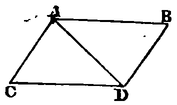
\includegraphics[width= 0.7\linewidth]{Fig/177px-Principia1846-084.png}
\caption{Figura utilizada por Newton para explicar a composição da ação de duas forças  considerando o deslocamento causado por elas dentro de um um intervalo de tempo $\Delta t$ e partindo de uma velocidade nula. Se uma força atuando isoladamente causa um deslocamento de $A$ até $B$ e a outra causa o deslocamento de $A$ até $C$, então ambas atuando conjuntamente causam o deslocamento de $A$ até $D$. Note que a figura denota a soma de dois vetores, como verificado no Capítulo~\ref{Chap:Vetores}.\label{Fig:ComposicaoForcasNewton}}
\end{marginfigure}


\noindent{}O conceito de força em Física é bastante próximo do que entendemos por força na vida cotidiana. Por exemplo, sabemos que para cada direção e sentido da força que aplicamos sobre um objeto, temos movimentos diferentes\footnote{Considerando que o corpo possa se mover livremente. Em um sistema que podem atuar diversas forças, algumas delas podem sofrer alteração ao exercermos uma força adicional, mantendo o sistema em equilíbrio. Verificaremos mais adiante como proceder nessas situações.}. Sabemos ainda que a composição de dois esforços, em laterais diferentes de um objeto, dá origem a um movimento diagonal (Figura~\ref{Fig:ComposicaoForcasNewton}). Tais características indicam que as forças são vetores, pois possuem módulo (intensidade da força), direção e sentido.

Sobre a massa, Newton afirma que ela é uma \emph{medida da quantidade de matéria}. Veremos que ela atuará como uma constante de proporcionalidade entre a força aplicada sobre um corpo, e a aceleração experimentada por ele. Ao contrário da força, a massa é uma quantidade escalar, por isso sua determinação no caso de um sistema composto por vários corpos é bastante simples: basta somarmos os valores de massa de cada um dos membros do sistema. Além disso, tal grandeza é estritamente positiva, não havendo valores negativos, ou mesmo nulos. Em alguns casos, no entanto podemos considerar que a massa de um corpo é desprezível em comparação com a de outros corpos.

Note que não definimos nenhuma unidade para a massa ou para a força. Faremos isso na Seção~\ref{Sec:SegundaLeiDeNewton}, pois precisaremos das Leis de Newton para definir as unidades e métodos para aferir os valores dessas grandezas.

%%%%%%%%%%%%%%%%%%%%%%%%%%%%%%%%%%%%%%%%%%%%%%%%%%%
\paragraph{Discussão: Diferença entre massa e peso}
%%%%%%%%%%%%%%%%%%%%%%%%%%%%%%%%%%%%%%%%%%%%%%%%%%%

Cabe aqui uma discussão acerca da confusão entre massa e peso. Newton deixa claro\footnote{Verifique os enunciados de Newton na Seção~\ref{Sec:EnunciadosNewton}} que a massa é uma medida da quantidade de matéria que um corpo possui, e que tal grandeza é \emph{proporcional} ao peso. Veja que o peso de um corpo possui características vetoriais, pois é dirigido verticalmente para baixo e possui um módulo que é tão maior quanto maior for sua quantidade de matéria, ou seja, quanto maior for a massa. Além disso, como veremos adiante, um corpo que se encontra longe da superfície da Terra é atraído por uma força que varia com a distância de separação, sendo, portanto diferente para cada posição. A massa, por outro lado, é uma constante característica do corpo e não está sujeita a mudanças, exceto se o corpo perde matéria.

%\textbf{Melhorar essa discussão.}

%%%%%%%%%%%%%%%%%%%%%%%%%%%%%%%%%%%%%%%%%%%%%%%%%%%%%%%%%%%%%%%%%%%%%%%%%%%%%%%%%%%%%%%%%%
\subsection{Primeira Lei de Newton: Princípio da Inércia segundo Galileu e segundo Newton}
%%%%%%%%%%%%%%%%%%%%%%%%%%%%%%%%%%%%%%%%%%%%%%%%%%%%%%%%%%%%%%%%%%%%%%%%%%%%%%%%%%%%%%%%%%

Ao analisar o movimento, Galileu em seu \emph{Diálogo sobre os dois principais sistemas do mundo} tece as seguintes observações:\footnote{O texto completo se encontra na Seção~\ref{Sec:TextoDialogo}}
\begin{itemize}

\begin{marginfigure}
\centering
\begin{tikzpicture}[>=Stealth,rotate = 30]

    \draw (0,0) -- (4,0);
    \draw[fill] (1,0.1) circle (1mm);
    \draw[->] (1,0.1) -- node[above, sloped]{$\vec{v}_f$} +(-0.8,0);
    \draw[fill] (3,0.1) circle (1mm);
    \draw[->] (3,0.1) -- node[above, sloped]{$\vec{v}_i$} +(-0.3,0);
    
\end{tikzpicture}
\caption{Um corpo que pode se mover livremente em uma rampa se desloca em direção ao ponto mais baixo e ganha velocidade durante o movimento.}
\end{marginfigure}
  \item Tomamos uma superfície inclinada lisa e resistente, juntamente com uma esfera também lisa e resistente e colocamos a segunda sobre a primeira, de forma que fique livre para rolar, tomando cuidado para remover todos os possíveis ``impedimentos'' ao movimento. Desprezamos também a resistência do ar. Observamos que a esfera rola em direção à parte mais baixa da superfície, ganhando velocidade continuamente enquanto dura a descida. Quanto maior a inclinação do plano em relação à horizontal, maior é o ganho de velocidade da esfera após percorrer uma dada distância.
  
\begin{marginfigure}[5mm]
\centering
\begin{tikzpicture}[>=Stealth, rotate = 30]

    \draw (0,0) -- (4,0);
    \draw[fill] (1,0.1) circle (1mm);
    \draw[->] (1,0.1) -- node[above, sloped]{$\vec{v}_i$} +(0.8,0);
    \draw[fill] (3,0.1) circle (1mm);
    \draw[->] (3,0.1) -- node[above, sloped]{$\vec{v}_f$} +(0.3,0);
    
\end{tikzpicture}
\caption{Ao lançarmos um corpo rampa acima, sua velocidade diminui progressivamente.}
\end{marginfigure}
  \item Para que a esfera suba o plano, é necessário que ela seja atirada com velocidade, ou arrastada, plano acima. Sendo atirada, o seu movimento natural é perder velocidade continuamente, eventualmente parando. Se aumentamos ou diminuímos a inclinação do plano, mantendo constante a velocidade com que a esfera foi atirada, temos que ela percorrerá uma distância maior ou menor, sendo tanto maior quanto menor for a inclinação e vice-versa.

\begin{marginfigure}[15mm]
\centering
\begin{tikzpicture}[>=Stealth]

    \draw (0,0) circle (2cm);
    \draw[fill] (0,2.1) circle (1mm);
    \draw[->] (0,2.1) -- node[above]{$\vec{v}$} +(1,0);
    \draw[dashed] (0,2.1) arc [start angle=90, end angle=0, radius=2.1cm];
    
\end{tikzpicture}
\caption{Um a superfície horizontal infinita é, na verdade, uma esfera perfeitamente lisa.}
\end{marginfigure}
  \item Se tomarmos uma superfície perfeitamente horizontal, não existe tendência a ganhos de velocidade, nem de perdas de velocidade. Se colocarmos a esfera de forma que ela fique parada sobre a superfície, ela deve permanecer parada. Se a colocarmos em movimento, não havendo impedimentos, ela deve permanecer em movimento. Não havendo inclinação do plano, não há razão para haver aumento ou diminuição da velocidade. Se o plano horizontal for infinito, ela deve continuar nesse movimento indefinidamente. A razão disto é que existe uma tendência dos corpos a se moverem em direção ao centro da Terra. Como em um plano horizontal todas as partes estão à mesma distância em relação ao centro, não existe um lugar preferencial da superfície para o qual a esfera tem uma tendência a se dirigir. Tal superfície seria, na realidade, uma esfera lisa e concêntrica com a Terra. Uma vez posta em movimento em direção ao norte, por exemplo, a esfera continuaria a se mover em tal direção até atingi-lo e passar a se mover para o sul, descrevendo um circulo em torno da Terra.
\end{itemize}
%
Portanto, podemos afirmar que ---~segundo Galileu~--- \emph{um corpo sobre uma superfície horizontal continuará se movendo na mesma direção com velocidade constante a não ser que seja perturbado}, o que é conhecido como \emph{princípio da inércia}. Devemos destacar que para Galileu, \emph{o movimento horizontal do corpo não é retilíneo}, mas um círculo em torno da Terra.\footnote[][-3cm]{Essa é a interpretação mais comum das principais obras de Galileu, porém há controvérsias sobre isso: veja \fullcite{VASCONCELOS2005}.} Finalmente, através de tais observações, Galileu concluiu que é impossível distinguir um corpo em movimento com velocidade constante de outro parado, a não ser que tenhamos uma referência externa.

No \emph{Principia}, Newton declara a primeira lei do movimento como:
\begin{quote}
  Todo corpo permanece em estado de repouso, ou de movimento uniforme em uma linha reta, a não ser que seja compelido a mudar tal estado por forças que atuam sobre ele.
\end{quote}
%
A diferença fundamental em relação ao proposto por Galileu é o fato de que o movimento, na ausência de forças, se dá em \emph{linha reta}. Verificamos no Capítulo~\ref{Chap:MovimentoBidimensional} que se temos uma mudança na direção da velocidade, temos uma aceleração, mesmo que o módulo do vetor velocidade se mantenha constante. Veremos através da Segunda Lei de Newton, a seguir, que se não temos forças, não temos aceleração. Consequentemente, na ausência de forças atuando sobre um corpo que se desloca, o movimento deve ser retilíneo e com o módulo da velocidade constante.

%\textbf{Inserir algum indicador para uma discussão opcional acerca de referenciais inerciais no final do capítulo.}

%%%%%%%%%%%%%%%%%%%%%%%%%%%%%%%%%%
\subsection{Segunda Lei de Newton}
\label{Sec:SegundaLeiDeNewton}
%%%%%%%%%%%%%%%%%%%%%%%%%%%%%%%%%%

Através da Primeira Lei de Newton, damos um passo adiante no estudo do movimento dos corpos, associando força à aceleração. Na Segunda Lei, Newton dá uma forma mais precisa para a dependência entre aceleração e força:
\begin{quote}
  A alteração do movimento é sempre proporcional à força motriz a ele aplicada; e é feita na direção da linha reta em que tal força atua.\footnote{Newton usa o termo \emph{movimento} para o que conhecemos hoje como \emph{quantidade de movimento} ou \emph{momento linear}, representado por $\vec{p}$. Tal definição, dada por $\vec{p} = m\vec{v}$ engloba tanto a massa quanto a velocidade, sendo que sua alteração pode se dar por meio de uma \emph{variação} da massa ou da velocidade (ou ambas, conjuntamente), ou seja, sua alteração se dá através da aceleração, se $m$ for mantido constante. Veremos mais sobre isso no Capítulo~\ref{Chap:CentroDeMassaEMomentoLinear}.}
\end{quote}

Nas seções seguintes, vamos explorar a relação enunciada, colocando-a em uma forma matemática. Após isso, vamos explorar as propriedades de forças que são comuns a fenômenos no contexto de mecânica, empregando esses conhecimentos na solução de prolemas simples.
 
%%%%%%%%%%%%%%%%%%%%%%%%%%%%%%%%%%%%%%%%%%%%
\paragraph{Relação entre força e aceleração}
%%%%%%%%%%%%%%%%%%%%%%%%%%%%%%%%%%%%%%%%%%%%

Experimentalmente, podemos verificar que a aceleração de um objeto é maior caso a força que exercemos sobre ele seja maior. Se temos uma alteração da velocidade quando um corpo se desloca por certo tempo sob ação de uma força, ao dobrarmos ou triplicarmos a intensidade da força, teremos que a alteração da velocidade dobrará ou triplicará no mesmo tempo, respectivamente. Podemos então dizer que\footnote{O símbolo $\propto$ denota \emph{proporcionalidade}.}
\begin{equation}
  a \propto F,
\end{equation}
%
ou, considerando que ---~como explicitado por Newton~--- a alteração é sempre na mesma direção que a força motriz,
\begin{equation}
    \vec{a} \propto \vec{F}.
\end{equation}
%
Note que a proporcionalidade implica em uma relação \emph{linear} entre a aceleração e a força aplicada.

\begin{marginfigure}[-1cm]
\centering
\begin{tikzpicture}[>=Stealth]

    \draw[->] (0,0) -- (4,0) node[below left]{$F$};
    \draw[->] (0,0) -- (0,2.5) node[below left]{$a$};
    
    \draw[thick] (0,0) -- (35:3);
    
\end{tikzpicture}
\caption{A relação de proporcionalidade entre $a$ e $F$ implica em uma relação linear entre tais grandezas.}
\end{marginfigure}

%%%%%%%%%%%%%%%%%%%%%%%%%%%%%%%%%%%%%%%%%%%%
\paragraph{Relação entre massa e aceleração}
%%%%%%%%%%%%%%%%%%%%%%%%%%%%%%%%%%%%%%%%%%%%

Como verificamos acima, se aplicarmos uma força em um corpo, observamos que ele estará sujeito a uma aceleração. No entanto, se aplicarmos uma dada força em um corpo muito massivo, teremos uma aceleração pequena, ao passo que se aplicarmos tal força em um corpo com uma massa pequena, teremos uma aceleração maior.

Se, por exemplo, aplicarmos uma força $F_1$ a um corpo de massa $m_1$, experimentalmente observaremos uma aceleração $a_1$. Ao submetermos um outro corpo, de massa $m_2 = 2 m_1$, à mesma força $F_1$, observamos experimentalmente que a aceleração $a_2$ corresponde à metade do valor de $a_1$. Se submetermos um corpo com massa $m_3 = 3 m_1$ a ação da força $F_1$, observamos uma aceleração $a_3$ que corresponde a um terço da aceleração $a_1$. Percebemos então que a aceleração assume uma proporcionalidade inversa em relação à massa:
\begin{equation}
  a \propto \frac{1}{m}.
\end{equation}

\begin{marginfigure}
\centering
\begin{tikzpicture}[>=Stealth]

    \draw[->] (0,0) -- (4,0) node[below left]{$m$};
    \draw[->](0,0) -- (0,2.5) node[below left]{$a$};
    
    \draw[smooth, thick, samples=1000, domain=0.1:3.5]
        plot (\x, {0.2 * 1/\x});
    
\end{tikzpicture}
\caption{A relação entre $a$ e $m$ é a de que a primeira é proporcional ao inverso da segunda.}
\end{marginfigure}

%%%%%%%%%%%%%%%%%%%%%%%%%%%%%%%%%%%%%%%%%%%%%%%%%%%%
\paragraph{Relação entre aceleração, força, e massa}
%%%%%%%%%%%%%%%%%%%%%%%%%%%%%%%%%%%%%%%%%%%%%%%%%%%%

Observando a dependência em relação à força, à massa, e o caráter vetorial das grandezas, temos que
\begin{equation}
  \vec{a} \propto \frac{\vec{F}}{m}.
\end{equation}
%
Considerando que a aceleração só dependa de $\vec{F}$ e $m$, e também o fato de que uma proporcionalidade pode ser escrita como uma igualdade se utilizarmos uma constante de proporcionalidade $C$ qualquer ---~cujo valor precisamos determinar~---, obtemos
\begin{equation}
  \vec{a} = C \frac{\vec{F}}{m}.
\end{equation}

Apesar de termos unidades para a aceleração e para a massa,\footnote{Veremos as unidades para a massa adiante.} não temos para a força. Nesse caso, podemos englobar a constante $C$ na própria definição das unidades da força e obter
\begin{equation}\label{Eq:SegundaLeiDeNewton}
  \vec{a} = \frac{\vec{F}}{m}. \mathnote{Segunda Lei de Newton.}
\end{equation}

A forma acima não é a mais conhecida, mas sim 
\begin{equation}
  \vec{F} = m \vec{a}.
\end{equation}
%
Matematicamente, as expressões são completamente equivalentes, porém a Equação~\ref{Eq:SegundaLeiDeNewton} deixa mais evidente a relação causa e efeito: a existência de uma força \emph{causa} uma aceleração.\footnote{A inversão dessa relação de causa e efeito é particularmente problemática ao tratarmos de forças no movimento circular, onde um erro comum é achar que existe uma força \emph{adicional} em movimentos circulares, denominada como \emph{força centrípeta}. Na verdade, alguma força, ou componente de força, ou mesmo uma combinação de forças e componentes, exerce o papel de força centrípeta e \emph{causa} o movimento circular. Discutiremos isso em detalhes adiante.} Note ainda que, de acordo com o que verificamos na Seção~\ref{Sec:OpAtravesDeComp}, podemos tratar a multiplicação de um vetor por um escalar através das componentes vetoriais nos três eixos de um sistema de referência ortogonal:
\begin{equation}
\begin{system}
F_x &= m a_x \\
F_y &= m a_y \\
F_z &= m a_z.
\end{system}
\end{equation}

%%%%%%%%%%%%%%%%%%%%%%%%%%%%%%
\paragraph{Forças resultantes}
%%%%%%%%%%%%%%%%%%%%%%%%%%%%%%

Até aqui consideramos o efeitos de forças atuando individualmente em um corpo. No entanto, como mencionado na Seção~\ref{Sec:ConceitosDeMassaEForca}, a composição da ação de duas forças ao mesmo tempo apresenta as propriedades de uma soma vetorial. Assim, quando duas ou mais forças atuam sobre um corpo, a aceleração estará relacionada à \emph{força resultante} $\vec{F}_R$, dada pela soma vetorial de todas as forças que atuam sobre o corpo:
\begin{equation}
    \vec{a} =\frac{\vec{F}_R}{m},
\end{equation}
%
onde,
\begin{align}
    \vec{F}_R &= \vec{F}_1 + \vec{F}_2 + \dots \\
    &= \sum_{i = 1}^n \vec{F}_i.
\end{align}
%
Note que se a soma das forças resulta em um \emph{vetor nulo}, temos uma aceleração \emph{nula}. Em tal situação, dizemos que o sistema se encontra em \emph{equilíbrio}.

%%%%%%%%%%%%%%%%%%%%%%%%%%%%%%%%%%%%%%%%%
\paragraph{Discussão: Unidades e medidas}
%%%%%%%%%%%%%%%%%%%%%%%%%%%%%%%%%%%%%%%%%

Através da Segunda Lei de Newton, podemos determinar a massa de um objeto em relação à massa de outro. Suponha que tomamos um objeto qualquer e a ele aplicamos uma força resultante $F$. Sabemos que ele será submetido a uma aceleração de tal maneira que
\begin{equation}
  F = m_1 a_1.
\end{equation}
%
Se submetermos outro corpo à mesma força,\footnote{É mais fácil falar isso do que fazer. Ainda não discutimos um dispositivo que nos permita medir forças, mas isso é relativamente simples de se fazer ao empregarmos uma mola: veremos adiante que a força exercida por uma mola é proporcional à distensão que ela sofre. Assim, é possível elaborar um equipamento simples ---~um dinamômetro~--- que consiste em uma mola associada a uma escala graduada, através da qual verificamos a força exercida pela mola.} temos
\begin{equation}
  F = m_2 a_2.
\end{equation}
%
Como a força é a mesma em ambos os casos, podemos escrever
\begin{equation}
  m_1 a_1 = m_2 a_2,
\end{equation}
%
ou
\begin{equation}
  m_2 = \frac{a_1}{a_2}m_1.
\end{equation}

Este resultado é relevante pois não temos um método de determinar a massa de um objeto a não ser por comparação com outro. Utilizando o processo acima, podemos determinar a massa de um objeto qualquer em relação ao padrão de referência.\footnote{ No Sistema Internacional (SI), até maio de 2019 se utiliza a massa de um cilindro metálico como massa padrão em relação a qual as demais massas são medidas, sendo atribuída a ele a massa de \np[kg]{1}. Atualmente, adotou-se que a \emph{constante de Planck} tem um valor exato $h = \np[J\cdot s]{6.62607015E-34}$. Como a unidade $\textrm{J}\cdot\textrm{s}$ equivale a $\textrm{kg}\cdot\textrm{m}^2/\textrm{s}$, ao definirmos o valor de $h$ e utilizarmos as definições de metro e de segundo, temos um valor específico para o $\textrm{kg}$.}

No caso das forças, as unidades do SI são
\begin{align}
    [F] &= [m a] \\
    &= [m] [a] \\
    &= \rm{kg} \frac{\rm{m}}{\rm{s}^2} \\
    &\equiv \rm{N},
\end{align}
%
onde utilizamos a definição $\rm{N} \equiv \rm{kg}\cdot\rm{m}/\rm{s}^2$ para nomear a unidade da força como \emph{Newton}, isto é, $\np[N]{1} \equiv \np[kg\cdot m/s^2]{1}$. Em princípio, podemos verificar o valor de uma força simplesmente determinando a massa de um corpo e o valor da aceleração a qual ele está sujeito quando sob ação de tal força.\footnote{Novamente, na prática usamos um dinamômetro para medir forças.}

%%%%%%%%%%%%%%%%%%%%%%%%%%%%%%%%%%%%%%%%%%%%%%%%%%%%%%%%%%%%%%%%%%%%%%%%%%%%%%%%
\subsection{Diagramas de forças, sistemas de referência, aplicações}
\label{Sec:DiagramaDeForcasESisDeRef}
%%%%%%%%%%%%%%%%%%%%%%%%%%%%%%%%%%%%%%%%%%%%%%%%%%%%%%%%%%%%%%%%%%%%%%%%%%%%%%%%

\begin{marginfigure}[3cm]
\centering
\begin{tikzpicture}[>=Stealth,
     interface/.style={
        % superfície
        postaction={draw,decorate,decoration={border,angle=-45,
                    amplitude=0.2cm,segment length=2mm}}},
    ]
    
    \draw[interface] (-1,0) -- (1,0);
    
    \draw[pattern= north west lines] (-0.5,0) rectangle (0.5,1);
    \draw[fill] (0,0.5) circle (1pt);
    
    \draw[dashed,->] (-1, 0.5) -- (1, 0.5) node[above left]{$x$};
    \draw[dashed,->] (0,-1) -- (0,2.5) node[below right]{$y$};
    
    \draw[->, thick] (0, 0.5) -- (0,-0.5) node[left]{$\vec{P}$};
    \draw[->, thick] (0,1) -- (0,2) node[left]{$\vec{N}$};
    
    \draw[fill] (2,0.5) circle (1pt);
    \draw[->, thick] (2,0.5) -- +(0,1) node[right]{$\vec{N}$};
    \draw[->, thick] (2,0.5) -- +(0,-1) node[right]{$\vec{P}$};
    
    \draw[dashed, ->](1.5,0.5) -- (2.5, 0.5) node[above left]{$x$};
    \draw[dashed, ->](2,-1) -- (2,2.5) node[below right]{$y$};
    
\end{tikzpicture}
\caption{Esboço de um problema e o diagrama de forças correspondente. Apesar de a rigor devermos utilizar o diagrama, é mais ilustrativo utilizar a representação da esquerda, porém ela tem problemas conceituais: a força $\vec{N}$ exercida pela mesa é exercida na parte inferior do bloco, não no topo, como ilustrado.\label{Fig:DiagramaDeForcasEEsboco}}
\end{marginfigure}

Um artifício fundamental para a interpretação e solução de problemas de dinâmica é o \emph{diagrama de corpo livre}, ou \emph{diagrama de forças}. Tal diagrama consiste em representar cada corpo como um ponto, sendo que todas as forças que atuam em tais corpos são representadas como atuando sobre o respectivo ponto (veja a parte à direita na Figura~\ref{Fig:DiagramaDeForcasEEsboco}). Além disso, não devemos incluir acelerações, velocidades, ou quaisquer outros vetores no diagrama de forças.

Podemos, ao invés de utilizar um diagrama de forças como descrito acima, fazer um esboço da situação (veja a parte à esquerda na Figura~\ref{Fig:DiagramaDeForcasEEsboco}). Isso em geral é mais interessante, pois ele reúne as principais características de um diagrama de forças e ao mesmo tempo permite uma visualização do problema. Esse artifício exige algumas adaptações, como representar forças em posições diferentes das ideais para que elas possam ser representadas confortavelmente no esboço.

Como já vimos, trabalhar com vetores é mais simples se utilizarmos um \emph{sistema de referência} no qual eles podem ser decompostos. A escolha da direção dos eixos é muito importante, pois um sistema inadequado pode dificultar muito a solução de um problema. Para uma escolha adequada, devemos observar os seguintes pontos:
\begin{itemize}
    \item Como regra geral, se houver aceleração no sistema, devemos escolher um dos eixos na direção de tal aceleração, pois assim teremos aceleração nula nos demais eixos. Em algumas situações, pode não ser possível saber de antemão qual será a direção da aceleração. Nesse caso, devemos observar os pontos adiante e escolher um sistema de coordenadas. O que provavelmente ocorrerá é termos componentes da aceleração em mais que um eixo.
    \item Caso não haja nenhuma aceleração, devemos verificar informações dadas sobre ângulos e procurar estabelecer eixos de forma que os ângulos entre as forças e os eixos sejam conhecidos.
    \item Finalmente, devemos procurar eixos que minimizem o número de forças que devem ser decompostas, isto é, devemos minimizar o número de forças que terão projeções em mais de um eixo.
\end{itemize}

\begin{marginfigure}[3cm]
\centering
\begin{tikzpicture}[>=Stealth]
    \draw[pattern = north west lines] (0,0) circle (0.25);

    \draw[dashed,->] (-2,0) -- (-0.25,0) (0.25,0) -- (2,0) node[below left]{$x$};
    \draw[dashed,->] (0,-2) -- (0,-0.25) (0,0.25) -- (0,2) node[below left]{$y$};
        
    \draw[->, thick] (45:0.25) coordinate (BL) -- (45:1.5) coordinate (F) node[right]{$\vec{F}_1$};
    \draw[->, thick] (-90:0.25) -- +(0,-1) node[right]{$\vec{F}_2$};
    \draw[->, thick] (180:0.25) -- +(-1,0) node[above]{$\vec{F}_3$};
    
    \draw[dotted] (45:0.25) -- +(1,0) coordinate (X);
    
    \pic[draw, "$\theta$", angle eccentricity = 1.5]{angle = X--BL--F};
\end{tikzpicture}
\caption{Um corpo submetido a um conjunto de forças. Note que devido à escolha da orientação do sistema de referência, as componentes $F_{2, x}$ e $F_{3, y}$ são nulas.\label{Fig:ExemploSisRefDecompForcas}}
\end{marginfigure}


Uma vez escolhido um sistema de referência, devemos aplicar a Segunda Lei de Newton a cada corpo separadamente, uma vez para cada eixo de referência. Se, por exemplo, tivermos uma situação como a da Figura~\ref{Fig:ExemploSisRefDecompForcas}, obtemos ao aplicar a Segunda Lei de Newton para cada eixo:
\begin{description}
    \item[Eixo $x$:]
        \begin{align}
            F_{R, x} &= ma_x \\
            F_{1, x} + F_{2, x} + F_{3, x} &= m a_x
        \end{align}
    \item[Eixo $y$:]
        \begin{align}
            F_{R, y} &= ma_x \\
            F_{1, y} + F_{2, y} + F_{3, y} &= m a_y,
        \end{align}            
\end{description}
%
onde as componentes das forças devem ser determinadas observando o que foi discutido no Capítulo~\ref{Chap:Vetores}.

A partir das equações obtidas, devemos buscar as informações que necessitamos, e que podem ser qualquer uma das variáveis presentes nas duas equações acima. Muitas vezes será necessário determinar duas informações de um mesmo conjunto do equações, por isso vamos precisar elaborar sistemas de equações para que possamos determinar tais informações.\footnote{É muito comum que ao se obter a aceleração, outras informações possam ser determinadas de maneira relativamente simples. Por isso, determinar a aceleração costuma ser o primeiro passo na solução de problemas, exceto ---~é claro~--- naqueles que envolvem equilíbrio.}

Devemos notar ainda que muitas vezes não sabemos de antemão qual será o \emph{sentido} da aceleração. Nesse caso, devemos simplesmente assumir qualquer um dos dois sentidos possíveis como sendo positivo. Ao resolvermos as equações, se estivermos interessados em calcular a aceleração, a obtenção de um valor negativo indica que a essa variável tem o sentido oposto àquele que assumimos.


%%%%%%%%%%%%%%%%%%%%%%%%%%%%%%%%%%%%%%%%%%%%%%%%%%%%%%%
\paragraph{Discussão: Sistemas em equilíbrio de forças}
%%%%%%%%%%%%%%%%%%%%%%%%%%%%%%%%%%%%%%%%%%%%%%%%%%%%%%%

\begin{marginfigure}[3cm]
\centering
\begin{tikzpicture}[>=Stealth]
    \draw[pattern = north west lines] (0,0) rectangle (1,1);
    
    \draw[->, thick] (1,1) coordinate (BL) -- +(1,1) coordinate (F) node[right]{$\vec{F}_1$};
    \draw[->, thick] (0.5,0) -- +(0,-1) node[right]{$\vec{F}_2$};
    \draw[->, thick] (0,0.5) -- +(-1,0) node[above]{$\vec{F}_3$};
    
    \draw[dashed] (1,1) -- +(1,0) coordinate (X);
    
    \pic[draw, "$\theta$", angle eccentricity = 1.5]{angle = X--BL--F};
\end{tikzpicture}
\caption{Um corpo submetido a um conjunto de forças e em equilíbrio.\label{Fig:ExemploEquilibrio}}
\end{marginfigure}

Uma situação particularmente comum é quando a força resultante sobre um corpo é nula. Nesse caso, temos o que chamamos de um \emph{sistema em equilíbrio}. Através da Segunda Lei de Newton, verificamos que a aceleração do corpo nessa situação é zero:
\begin{align}
    \vec{a} &= \frac{\vec{F}_R}{m} \\
    &= 0.
\end{align}
%
Note que o equilíbrio não significa que a velocidade é necessariamente zero, pois uma velocidade constante em módulo e direção satisfaz a condição de ``aceleração nula'' perfeitamente.

\begin{marginfigure}[2cm]
\centering
\begin{tikzpicture}[>=Stealth]
    \draw[pattern = north west lines] (0,0) rectangle (1,1);
    
    \draw[->, thick] (1,1) coordinate (BL) -- +(1,1) coordinate (F1) node[right]{$\vec{F}_1$};
    \draw[->, thick] (0.5,0) -- +(0,-1) node[right]{$\vec{F}_2$};
    \draw[->, thick] (0,0.5) -- +(-1,0) node[above]{$\vec{F}_3$};
    
    \draw[->, dashed] (-1.5,0.5) -- (2.5,0.5) node[below left]{$x$};
    \draw[->, dashed] (0.5, -1.5) -- (0.5, 2) node[below left]{$y$};
    
    \draw[dashed] (1,1) -- +(1,0) coordinate (X);
    \pic[draw, "$\theta$", angle eccentricity = 1.5] {angle = X--BL--F1};
\end{tikzpicture}
\caption{Um corpo submetido a um conjunto de forças e em equilíbrio.\label{Fig:ExemploEquilibrioRef}}
\end{marginfigure}

Na Figura~\ref{Fig:ExemploEquilibrio} temos um corpo sujeito a um conjunto de forças e em equilíbrio. Podemos determinar a relação entre as forças através da Segunda Lei de Newton. Para isso, vamos adotar um sistema de referência e determinar o ângulo entre as forças e os eixos. Veja a Figura~\ref{Fig:ExemploEquilibrioRef}. Aplicando a Segunda Lei de Newton a cada eixo, temos:
\begin{description}
    \item[Eixo $x$:]
        \begin{align}
            F_{R, x} &= m a_x \\
            F_{1, x} + F_{2, x} + F_{3, x} &= 0 \label{Eq:PassoComponentesVetoresSegundaLeiX}\\
            F_{1, x} - F_3 &= 0 \\
            F_{1, x} &= F_3.
        \end{align}
    \item[Eixo $y$:]
        \begin{align}
            F_{R, y} &= m a_y \\
            F_{1, y} + F_{2, y} + F_{3, y} &= 0 \label{Eq:PassoComponentesVetoresSegundaLeiY}\\
            F_{1, y} - F_2 &= 0 \\
            F_{1, y} &= F_2.
        \end{align}
\end{description}
%
Em ambos os eixos utilizamos o fato de que, se há equilíbrio no eixo, então a aceleração é nula. Note ainda que utilizamos para as componentes
\begin{align}
    F_{2, x} &= 0 \\
    F_{2, y} &= -F_2 \\
    F_{3, x} &= -F_3 \\
    F_{3, y} &= 0.
\end{align}
%
Tais resultados se devem ao fato de que temos projeções completas no sentido negativo do eixo (para $F_{2, y}$ e $F_{3, x}$), ou projeções nulas (para $F_{2, x}$ e $F_{3, y}$).\footnote{Por conveniência, geralmente o segundo passo nas expressões para os eixos $x$ e $y$, Equações~\eqref{Eq:PassoComponentesVetoresSegundaLeiX} e~\eqref{Eq:PassoComponentesVetoresSegundaLeiY}, não é escrito explicitamente. Passamos diretamente para o passo seguinte, onde já substituímos as projeções completas e as projeções nulas.}

A força $\vec{F}_1$ pode ser decomposta utilizando as funções trigonométricas e o fato de que o ângulo entre a força e o eixo $x$ é $\theta$, o que resulta em
\begin{align}
    F_1 \cos\theta &= F_3 \\
    F_1 \sen\theta &= F_2.
\end{align}

Note que a escolha do sistema de referências foi feita com base no ângulo dado e no fato de que as forças $\vec{F}_2$ e $\vec{F}_3$ não precisariam ser decompostas. No entanto, outros sistemas poderiam ser utilizados, desde que conseguíssemos determinar o ângulo entre cada força e os eixos de referência.

%%%%%%%%%%%%%%%%%%%%%%%%%%%%%%%%%%%%%%%%%%%%%%%%%%%%%%%%%%%%%%%%%%%%%%%%%%%%
\paragraph{Exemplo: Determinação de uma força em um sistema em equilíbrio}
%%%%%%%%%%%%%%%%%%%%%%%%%%%%%%%%%%%%%%%%%%%%%%%%%%%%%%%%%%%%%%%%%%%%%%%%%%%%

\begin{quote}
    Dada a Figura~\ref{Fig:ExemploEquilibrio2}, considerando que $\vec{F}_2 \perp \vec{F}_3$, $F_2 = \np[N]{15}$, $F_3 = \np[N]{10}$, e $\vec{a} = 0$, determine o módulo da força $\vec{F}_1$ e o ângulo que ela faz com a força $\vec{F}_2$.
\end{quote}

\begin{marginfigure}
\centering
\begin{tikzpicture}[>=Stealth, scale = 0.7]
    \draw[pattern = north west lines] (0.5,0.5) circle (0.5);
    
    \draw[->, thick] (0.5,0.5) +(-146.31:0.5) coordinate (BL) -- +(-146.31:1.8) coordinate (F) node[below]{$\vec{F}_1$};
    \draw[->, thick] (1,0.5) -- +(1.5,0) node[below left]{$\vec{F}_2$} coordinate (F2);
    \draw[->, thick] (0.5,1) -- +(0,1) node[below right]{$\vec{F}_3$};
    
    \coordinate (CM) at (0.5,0.5);
    
    \pic[draw, "$\theta$", angle eccentricity = 1.5, angle radius = 7mm]{angle = F--CM--F2};
\end{tikzpicture}
\caption{Um corpo submetido a um conjunto de forças e em equilíbrio.\label{Fig:ExemploEquilibrio2}}
\end{marginfigure}

Podemos determinar o módulo da força $\vec{F}_1$ e seu ângulo em relação a $\vec{F}_2$ aplicando a Segunda Lei de Newton e observando que a aceleração é zero por se tratar de uma situação de equilíbrio:
\begin{align}
    \vec{F}_R &= m \vec{a} \\
    &= 0.
\end{align}

\begin{marginfigure}[2cm]
\centering
\begin{tikzpicture}[>=Stealth, scale = 0.7]
    \draw[pattern = north west lines] (0.5,0.5) circle (0.5);

    \draw[dashed, ->] (0.5,1) -- +(0,1.75) node[below left]{$y$};
    \draw[dashed] (0.5,0) -- +(0,-1.75) coordinate (by);
    \draw[dashed] (0,0.5) -- +(-2,0);
    \draw[dashed,->] (1,0.5) -- +(2.5,0) node[below left]{$x$};
        
    \draw[->, thick] (0.5,0.5) +(-146.31:0.5) coordinate (BL) -- +(-146.31:1.8) coordinate (F) node[below]{$\vec{F}_1$};
    \draw[->, thick] (1,0.5) -- +(1.5,0) node[below left]{$\vec{F}_2$} coordinate (F2);
    \draw[->, thick] (0.5,1) -- +(0,1) node[below right]{$\vec{F}_3$};
    
    \coordinate (CM) at (0.5,0.5);
    
    \pic[draw, "$\alpha$", angle eccentricity = 1.5, angle radius = 7mm]{angle = F--CM--by};
    
\end{tikzpicture}
\caption{Um corpo submetido a um conjunto de forças e em equilíbrio.\label{Fig:ExemploEquilibrio2Ref}}
\end{marginfigure}

Para auxiliar a análise do problema, escolhemos o sistema de referência mostrado na Figura~\ref{Fig:ExemploEquilibrio2Ref}. Tal escolha se deu por ser o sistema de referência que minimiza o número de forças que tem componentes em ambos os eixos. Como determinado acima, a aceleração é nula, logo as componentes da aceleração nos eixos $x$ e $y$ também serão nulas,
\begin{align}
    a_x &= 0 \\
    a_y &= 0,
\end{align}
%
o que implica em
\begin{align}
    F_{R, x} &= 0 \\
    F_{R, y} &= 0.
\end{align}

Note que na Figura~\ref{Fig:ExemploEquilibrio2Ref} passamos a denotar o ângulo $\alpha$ entre o vetor $\vec{F}_3$ e o eixo $y$, uma vez que $\theta = \alpha + \np[\tcdegree]{90}$. As componentes de cada força nos eixos $x$ e $y$ podem ser determinadas através de uma decomposição de vetores. Para a força $\vec{F}_1$, em especial, podemos utilizar o ângulo $\alpha$ desde que os sinais sejam inseridos ``manualmente''.\footnote[][-3cm]{Note que as projeções do vetor $\vec{F}_1$ são negativas em ambos os eixos, porém $0 < \alpha < \degree{90}$, o que implica em $\sen\alpha > 0 $ e $\cos\alpha > 0$. Como o módulo de um vetor é sempre uma grandeza positiva, devemos inserir o sinal manualmente para que as projeções tenham sinais apropriados.} Assim, temos
\begin{align*}
    F_{1, x} &= -F_1\sen\alpha & F_{1, y} &= -F_1 \cos\alpha \\
    F_{2, x} &= F_2 & F_{2, y} &= 0 \\
    F_{3, x} &= 0 & F_{3, y} &= F_3.
\end{align*}
%
Note que as componentes de $\vec{F}_1$ são negativas, uma vez que as projeções apontam no sentido negativo dos eixos.\footnote[][-3cm]{Devemos destacar que os sinais mostrados têm de ser inseridos ``à mão'' pois estamos fazendo a decomposição através do ângulo $\alpha$. Se medíssemos o ângulo em relação ao eixo $x$, em sentido anti-horário, as próprias funções trigonométricas seno e cosseno já determinariam tais sinais, uma vez que para ângulos no terceiro quadrante ambas são negativas. No entanto, é muito comum ao se trabalhar com ângulos os restringir a valores do primeiro quadrante (note que $\alpha < \np[\tcdegree]{90}$). Nesse caso, devemos tomar o cuidado de inserir sinais adequados.}

Substituindo os valores das componentes nas expressões para a força resultante, obtemos
\begin{align}
    F_{R, x} &= F_{1, x} + F_{2, x} + F_{3, x} \\
    &= -F_1\sen\alpha + F_2 + 0 = 0 \\
    F_{R, y} &= F_{1, y} + F_{2, y} + F_{3, y} \\
    &= -F_1\cos\alpha + 0 + F_3 = 0,
\end{align} 
%
de onde podemos escrever o sistema de equações dado por
\begin{equation}
\begin{system}
    -F_1\sen\alpha + F_2 &= 0 \\
    -F_1\cos\alpha + F_3 &= 0.
\end{system}
\end{equation}
%
A solução do sistema pode ser feitas de diversas maneiras, mas para esse caso o caminho mais simples envolve reescrevê-lo como
\begin{equation}
\begin{system}
    F_1\sen\alpha &= F_2 \\
    F_1\cos\alpha &= F_3
\end{system}
\end{equation}
%
e dividir a primeira equação pela segunda, obtendo
\begin{align}
    \frac{F_1\sen\alpha}{F_1\cos\alpha} &= \frac{F_2}{F_3} \\
    \frac{\sen\alpha}{\cos\alpha} &= \frac{F_2}{F_3} \\
    \tan\alpha &= \frac{F_2}{F_3}.
\end{align}
%
Utilizando a função $\arctan$, temos
\begin{align}
    \alpha &= \arctan\frac{F_2}{F_3} \\
    &= \arctan\left(\frac{(\np[N]{15})}{(\np[N]{10})}\right) \\
    &= \degree{56,31} \\
    &= \np[\tcdegree]{56}.
\end{align}

Conhecendo o valor de $\alpha$, basta voltarmos a qualquer uma das duas equações do sistema e determinarmos o valor de $F_1$. Tomando a primeira delas, por exemplo, temos
\begin{align}
    F_1 \sen\alpha &= F_2 \\
    F_1 &= \frac{F_2}{\sen\alpha} \\
    &= \frac{(\np[N]{15})}{\sen(\degree{56,31})} \\
    &= \np[N]{18,03} \\
    &= \np[N]{18}.
\end{align}

%%%%%%%%%%%%%%%%%%%%%%%%%%%%%%%%%%%%%%%%%%%%%%%%%%%%%%%%%%%
\paragraph{Discussão: Sistema fora do equilíbrio de forças}
%%%%%%%%%%%%%%%%%%%%%%%%%%%%%%%%%%%%%%%%%%%%%%%%%%%%%%%%%%%

Toda situação onde não existe um perfeito equilíbrio das forças que atuam em um corpo implica na existência de uma aceleração. Se considerarmos, por exemplo, a situação mostrada na Figura~\ref{Fig:CorpoSujeitoForcasNaoEquilibrio}, verificamos a existência de quatro forças atuando sobre um corpo. As forças $\vec{F}_1$ e $\vec{F}_2$ são perpendiculares entre si, enquanto os ângulos entre $\vec{F}_3$ e $\vec{F}_2$, e entre $\vec{F}_4$ e $\vec{F}_2$ são $\theta$ e $\phi$, respectivamente. 

\begin{marginfigure}
\centering
\begin{tikzpicture}[>=Stealth]

    \draw[pattern = north west lines] (0.5,0.5) circle (0.5);
    
    \draw[->, thick] (0.5,1) -- +(0,1) node[left]{$\vec{F}_1$};
    \draw[->, thick] (1,0.5) -- +(1,0) node[below]{$\vec{F}_2$};
    \draw[->, thick] (0.5,0.5)++(-115:0.5) -- +(-115:0.8) node[left]{$\vec{F}_3$};
    \draw[->, thick] (0.5,0.5)++(40:0.5) -- +(40:0.5) node[above]{$\vec{F}_4$};
\end{tikzpicture}
\caption{Corpo sujeito a um conjunto de forças que não se encontram em equilíbrio.\label{Fig:CorpoSujeitoForcasNaoEquilibrio}}
\end{marginfigure}

Não há razão para assumimos que há equilíbrio em tal sistema, por isso devemos levar em conta a aceleração devida à força resultante. Para que possamos determinar o vetor aceleração mais facilmente, escolhemos o sistema de coordenadas mostrado na Figura~\ref{Fig:CorpoSujeitoForcasNaoEquilibrioRef}. A escolha da direção dos eixos se deu com base no fato de que dois dos vetores são nas direções dos eixos $x$ e $y$ escolhidos, e os outros dois vetores podem ser decompostos em tais eixos pois sabemos os ângulos entre cada um deles e o eixo $x$. Nesse sistema, vemos que é mais simples utilizar o ângulo $\alpha$ para descrever a direção do vetor $\vec{F}_3$, sendo que $\theta = \alpha + \np[\tcdegree]{90}$.

\begin{marginfigure}
\centering
\begin{tikzpicture}[>=Stealth]

    \draw[pattern = north west lines] (0.5,0.5) coordinate (center) circle (0.5);
    
    \draw[dashed, ->] (0.5,1) -- +(0,1.5) node[below right]{$y$};
    \draw[dashed] (0.5,0) -- +(0,-1.5) coordinate (yf);
    
    \draw[dashed] (0,0.5) -- +(-1.5,0);
    \draw[dashed, ->] (1,0.5) -- +(1.5,0) node[below left]{$x$};
    
    \draw[->, thick] (0.5,1) -- +(0,1) node[left]{$\vec{F}_1$} coordinate (F1);
    \draw[->, thick] (1,0.5) -- +(1,0) node[below]{$\vec{F}_2$} coordinate (F2);
    \draw[->, thick] (0.5,0.5)++(-115:0.5) -- +(-115:0.8) node[left]{$\vec{F}_3$} coordinate (F3);
    \draw[->, thick] (0.5,0.5)++(40:0.5) -- +(40:0.5) node[above]{$\vec{F}_4$} coordinate (F4);
    
    \pic[draw, "$\alpha$", angle eccentricity = 1.5, angle radius = 7mm]{angle = F3--center--yf};
    \pic[draw, "$\phi$", angle eccentricity = 1.5, angle radius = 7mm]{angle = F2--center--F4};

\end{tikzpicture}
\caption{Através de um sistema de referência, podemos determinar a aceleração resultante mais facilmente.\label{Fig:CorpoSujeitoForcasNaoEquilibrioRef}}
\end{marginfigure}

Aplicando a Segunda Lei de Newton para cada um dois eixos, temos
\begin{description}
\item[Eixo $x$:]
\begin{align}
    F_{R, x} &= m a_x \\
    F_{1, x} + F_{2, x} + F_{3, x} + F_{4, x} &= m a_x \\
    F_2 - F_3\sen\alpha + F_4 \cos\phi &= m a_x.
\end{align}

\item[Eixo $y$:]
\begin{align}
    F_{R, y} &= ma_y \\
    F_{1, y} + F_{2, y} + F_{3, y} + F_{4, y} &= m a_y \\
    F_1 + F_4 \sen\phi - F_3\cos\alpha &= m a_y.
\end{align}
\end{description}

Para que possamos determinar as componentes da aceleração, a partir desse ponto precisamos de valores numéricos específicos. Supondo que a massa do corpo seja de \np[kg]{2,0}, e que
\begin{align*}
    F_1 &= \np[N]{10} & F_3 &= \np[N]{8,0} \\
    F_2 &= \np[N]{10} & F_4 &= \np[N]{5,0} \\
    \phi &= \np[\tcdegree]{40} & \alpha &= \np[\tcdegree]{25},
\end{align*}
%
obtemos
\begin{align}
    m a_x &= (\np[N]{10}) + (\np[N]{5})\cdot(\cos \np[\tcdegree]{40}) - (\np[N]{8})\cdot(\sen \np[\tcdegree]{25}) \\
    m a_y &= (\np[N]{10}) + (\np[N]{5})\cdot(\sen \np[\tcdegree]{40}) - (\np[N]{8})\cdot(\cos \np[\tcdegree]{25})
\end{align}
%
o que resulta em
\begin{align}
    a_x &= \np[m/s^2]{5,2}\\
    a_y &= \np[m/s^2]{3,0},
\end{align}
%
ou, em termos dos vetores unitários,
\begin{equation}
    \vec{a} = \np[m/s^2]{5,2} \;\versi + \np[m/s^2]{3,0} \;\versj.
\end{equation}
%
Podemos ainda determinar o módulo da aceleração e o ângulo que ela faz com o eixo $x$, obtendo
\begin{align}
    a &= \np[m/s^2]{6,0}\\
    \beta &= \np[\tcdegree]{30}.
\end{align}

\begin{marginfigure}[-2cm]
\centering
\begin{tikzpicture}[>=Stealth]

    \draw[pattern = north west lines] (0.5,0.5) coordinate (center) circle (0.5);
    
    \draw[dashed, ->] (0.5,1) -- +(0,1.5) node[below right]{$y$};
    \draw[dashed] (0.5,0) -- +(0,-1.5) coordinate (yf);
    
    \draw[dashed] (0,0.5) -- +(-1.5,0);
    \draw[dashed, ->] (1,0.5) -- +(1.5,0) node[below left]{$x$};
    
    \draw[->, thick] (0.5,1) -- +(0,1) node[left]{$\vec{F}_1$} coordinate (F1);
    \draw[->, thick] (1,0.5) -- +(1,0) node[below]{$\vec{F}_2$} coordinate (F2);
    \draw[->, thick] (0.5,0.5)++(-115:0.5) -- +(-115:0.8) node[left]{$\vec{F}_3$} coordinate (F3);
    \draw[->, thick] (0.5,0.5)++(40:0.5) -- +(40:0.5) node[above]{$\vec{F}_4$} coordinate (F4);
    
    \draw[->] (0.5,0.5) ++(29.72:0.5) -- +(29.72:1.2) node[right]{$\vec{a}$} coordinate (a);
    
    \pic [draw, "$\beta$", angle eccentricity = 1.5, angle radius = 8mm] {angle = F2--center--a};

\end{tikzpicture}
\caption{Aceleração resultante da ação de um conjunto de forças em um corpo.\label{Fig:CorpoSujeitoForcasNaoEquilibrioRefAcel}}
\end{marginfigure}

%%%%%%%%%%%%%%%%%%%%%%
%\paragraph{Exemplo: ?}
%%%%%%%%%%%%%%%%%%%%%%

%\textbf{Um segundo exemplo numérico e com forças genéricas fora do equilíbrio. Pode ser um exemplo com diversas forças, de maneira que não seja possível saber de antemão em qual direção ocorrerá a aceleração. Assim obteremos uma aceleração que tem componentes nos dois eixos.}

%%%%%%%%%%%%%%%%%%%%%%%%%%%%%%%%%%%%%%%%%%%%%%%%%%%%%%%%%%%%%%%%%%%%%%%%%%%%%%%%%%%%%%%%%%%%%%%%%%
\paragraph{Discussão: Sistema fora do equilíbrio de forças, com a direção da aceleração conhecida}
%%%%%%%%%%%%%%%%%%%%%%%%%%%%%%%%%%%%%%%%%%%%%%%%%%%%%%%%%%%%%%%%%%%%%%%%%%%%%%%%%%%%%%%%%%%%%%%%%%

Em diversas situações, um sistema físico está sujeito a uma série de \emph{vínculos} que limitam o movimento a uma só direção. Dessa forma, se há aceleração, sua direção já é pré-determinada. Nesses casos, podemos obter uma grande simplificação do problema em questão se optarmos por um sistema de coordenadas em que a direção de um dos eixos é a própria direção da aceleração. Isso garante que os demais eixos possam ser tratados como uma situação de equilíbrio.

\begin{marginfigure}
\centering
\begin{tikzpicture}[>=Stealth]

    \draw[pattern = north west lines] (0,0) coordinate (center) circle (0.5);
    \draw (-2,0) -- (-0.5,0) (0.5,0) -- (2,0);
    
    \draw[->, thick] (45:0.5) -- (45:1.5) node[above]{$\vec{F}_1$} coordinate (F1);
    \draw[->, thick] (-90:0.5) -- (-90:1.5) node[left]{$\vec{F}_2$};
    
    \draw[->] (1.25, -0.3) -- node[below]{$\vec{a}$} +(0.75,0);
    
\end{tikzpicture}
\caption{Uma conta que se move ao longo de um fio é um exemplo de um movimento sujeito a um vínculo que determina a direção da aceleração.\label{Fig:ContaDeslisandoEmFio}}
\end{marginfigure}

Como exemplo de um sistema submetido a um vínculo, vamos considerar uma conta ---~isto é, uma pequena esfera perfurada~--- que pode deslizar ao longo de um fio. Vamos supor que a conta está sujeita a uma força $\vec{F}_1$ que faz um ângulo $\theta$ com a direção do fio, e a uma força $\vec{F}_2$ exercida pelo próprio fio sobre a conta, através da parede interna do orifício. Vamos considerar que a aceleração $a$ da conta e sua massa $m$ são conhecidas, além do ângulo $\theta$, e que procuramos os valores de $F_1$ e $F_2$.

Se a conta está sujeita a forças como mostrado na Figura~\ref{Fig:ContaDeslisandoEmFio}, devemos escolher um sistema de coordenadas em que um dos eixos aponta na própria direção do fio, pois esta é a direção da aceleração. Ao decompormos as forças e utilizarmos a Segunda Lei de Newton, obtemos:
\begin{description}
\item[Eixo $x$:] Para o eixo $x$ temos que $a_x \equiv a$, pois adotamos o eixo de referência $x$ na mesma direção da aceleração, logo,
\begin{align}
    F_{R, x} &= m a_x \\
    F_{1, x} + F_{2, x} &= m a \\
    F_1 \cos\theta &= m a \\
    F_1 &= \frac{ma}{\cos\theta}.
\end{align}

\item[Eixo $y$:] Nesse eixo não existe aceleração, logo $a_y \equiv 0$, portanto,
\begin{align}
    F_{R, y} &= m a_y \\
    F_{1, y} + F_{2, y} &= m a_y \\
    F_1\sen\theta - F_2 &= 0 \\
    F_2 &= F_1 \sen\theta.
\end{align}
\end{description}
%
Substituindo na expressão acima o resultado encontrado para $F_1$, determinamos o valor de $F_2$:
\begin{align}
    F_2 &= ma \frac{\sen\theta}{\cos\theta} \\
    F_2 &= ma\tan\theta.
\end{align}

\begin{marginfigure}
\centering
\begin{tikzpicture}[>=Stealth]

    \draw[pattern = north west lines] (0,0) coordinate (center) circle (0.5);
    \draw (-2,0) -- (-0.5,0);
    \draw[->] (0.5,0) -- (2,0) coordinate (x) node[above left]{$x$};
    
    \draw[dashed, ->] (0,0.5) -- +(0,1.5) node[below left]{$y$};
    \draw[dashed] (0,-0.5) -- +(0,-1.5);
    
    \draw[->, thick] (45:0.5) -- (45:1.5) node[above]{$\vec{F}_1$} coordinate (F1);
    \draw[->, thick] (-90:0.5) -- (-90:1.5) node[left]{$\vec{F}_2$};
    
    \draw[->] (1.25, -0.3) -- node[below]{$\vec{a}$} +(0.75,0);
    
    \pic [draw, "$\theta$", angle eccentricity = 1.5, angle radius = 7mm]{angle = x--center--F1};
\end{tikzpicture}
\caption{Ao escolhermos a direção de um dos eixos do sistema de referência como sendo aquela da aceleração, reduzimos a complexidade matemática do problema pois teremos uma situação de equilíbrio nos demais eixos.\label{Fig:ContaDeslisandoEmFioRef}}
\end{marginfigure}

Através das equações obtidas acima é possível verificar que a escolha de um sistema de referência com um dos eixos apontando na direção da aceleração nos leva a um sistema de equações cuja solução é mais simples, pois \emph{no eixo perpendicular à aceleração temos equilíbrio}. Note que a ideia de simplificar o tratamento matemático ao escolher a aceleração na direção de um dos eixos coordenados já foi utilizada no Capítulo~\ref{Chap:MovimentoBidimensional}, ao tratarmos o movimento de projéteis.

%%%%%%%%%%%%%%%%%%%%%%
%\paragraph{Exemplo: ?}
%%%%%%%%%%%%%%%%%%%%%%

%\textbf{Um exemplo numérico e com forças genéricas fora do equilíbrio}



%%%%%%%%%%%%%%%%%%%%%%%%%%%%%%%%%%%
\subsection{Terceira Lei de Newton}
%%%%%%%%%%%%%%%%%%%%%%%%%%%%%%%%%%%

A Terceira Lei de Newton foi por ele enunciada como
\begin{quote}
    Para cada ação há sempre uma reação igual oposta: ou as ações mutuas de dois corpos um sobre o outro são sempre iguais, e dirigidas a partes contrárias.
\end{quote}

\begin{marginfigure}
\centering
\begin{tikzpicture}[>=Stealth,
     interface/.style={
        % superfície
        postaction={draw,decorate,decoration={border,angle=-45,
                    amplitude=0.2cm,segment length=2mm}}},
    ]
    
    \draw[interface](-2,0) -- (2,0);
    
    \draw[pattern = north west lines, pattern color = gray] (-1,0) rectangle (0,1);
    \draw[pattern = north east lines, pattern color = gray] (0,1) rectangle (1,0);
    
    \draw[->,thick] (-2, 0.5) -- node[above]{$\vec{F}$} +(1,0);
    \draw[->,thick] (0,0.5) -- node [above]{$\vec{F}_{12}$} +(0.5,0);
    \draw[->,thick] (0,0.5) -- node [above]{$\vec{F}_{21}$} +(-0.5,0);
    
    \draw[->] (-0.5,1.25) -- node[above]{$\vec{a}$} +(1,0);
\end{tikzpicture}
\caption{Ao submetermos dois blocos a uma força $\vec{F}$, ocorrerá uma interação na superfície de contato entre eles. Tal interação resultará na força $\vec{F}_{12}$ para a direita atuando no bloco da direita, fazendo com que ele acelere, e na força $F' \equiv \vec{F}_{21}$ para a esquerda atuando no bloco da esquerda. No caso do bloco da esquerda a \emph{força resultante} $\vec{F}_R = \vec{F} - \vec{F}_{21}$ será a responsável pela aceleração.\label{Fig:ParAcaoReacao}}
\end{marginfigure}

\noindent{}Denominamos tal par como um \emph{par ação--reação}\footnote{Quem é a ação e quem é a reação é completamente irrelevante.}. Note que:
\begin{itemize}
    \item As forças do par nunca atuam sobre o mesmo corpo: em uma interação entre dois corpos quaisquer, uma delas, $\vec{F}_{12}$, atua sobre um dos corpos, enquanto a outra, $\vec{F}_{21}$, atua sobre o outro (Figura~\ref{Fig:ParAcaoReacao});
    \item As forças atuam na mesma direção, porém com sentidos opostos;
    \item As forças têm o mesmo módulo. A reação a uma força qualquer $\vec{F}$ é denotada como $\vec{F}'$, sendo que o módulo de ambas é denotado por $F$.\footnote{No exemplo da Figura~\ref{Fig:ParAcaoReacao}, podemos denotar $\vec{F}_{21}$ como $\vec{F}'_{12}$.}
\end{itemize}
%
Devemos notar ainda que Newton contempla a interação por quaisquer meios, seja por contato (Figura~\ref{Fig:ParAcaoReacao}), seja à distância (Figura~\ref{Fig:AcaoReacaoADistancia}).



\begin{marginfigure}
\centering
\begin{tikzpicture}[>=Stealth,
     interface/.style={
        % superfície
        postaction={draw,decorate,decoration={border,angle=-45,
                    amplitude=0.2cm,segment length=2mm}}},
    ]
    
    \draw[interface] (-2.5,0) -- (2.5,0);
    
    \draw (-2, 0) rectangle node[rotate=90]{N} (-1.5,0.5);
    \draw[fill] (-1.5,0.5) rectangle (-1,0);
    
    \draw (1, 0) rectangle node[rotate=90]{N} (1.5,0.5);
    \draw[fill] (1.5,0.5) rectangle (2,0);
    
    \draw[->,thick] (-1,0.25) -- node[above]{$\vec{F}_{12}$} +(0.75,0);
    \draw[->,thick] (1,0.25) -- node[above]{$\vec{F}_{21}$} +(-0.75,0);
    
    \draw[->] (-1.75,0.75) -- node[above]{$\vec{a}_1$} +(+0.5,0);
    \draw[->] (1.75,0.75) -- node[above]{$\vec{a}_2$} +(-0.5,0);
\end{tikzpicture}
\caption{Mesmo no caso de uma interação à distância, temos um par ação-reação: Na situação mostrada na figura, na ausência de atrito, ambos os imãs se deslocariam e estariam sujeitos a acelerações $a_1 = F/m_1$ e $a_2 = F/{m_2}$.\label{Fig:AcaoReacaoADistancia}}
\end{marginfigure}

%%%%%%%%%%%%%%%%%%%%%%%%%%%%%%%%%%%%%%%%%%%%%%%%%%%%%%%%%%%%%%%%%%%%%%%%%%%%%%%%%%%%%%%%%%
\paragraph{Discussão: Diferenças de aceleração entre dois corpos que interagem através de um par ação-reação}
%%%%%%%%%%%%%%%%%%%%%%%%%%%%%%%%%%%%%%%%%%%%%%%%%%%%%%%%%%%%%%%%%%%%%%%%%%%%%%%%%%%%%%%%%%

Muitas vezes, devido às diferentes massas dos corpos que interagem, pode ser difícil perceber que um deles está sujeito a uma força quando interage com outro. Se, por exemplo, um patinador arremessa uma bola com força, verificamos que a bola sofre uma grande alteração de sua velocidade. O patinador, por sua vez, sofre uma aceleração na mesma direção, porém com o sentido contrário.  Observamos, no entanto, que sua velocidade final é muito menor. Isto pode ser entendido através da Segunda Lei de Newton, pois, como as forças que atuam  em cada um dos corpos são iguais em módulo
\begin{align}
  F &= m_1 a_1 \\
  F' &= m_2 a_2
\end{align}
%
e, consequentemente,
\begin{equation}
  a_2 = \frac{m_1}{m_2} a_1.
\end{equation}
%
Logo, se supomos que a massa $m_1$ da bola é muito menor que a massa $m_2$ do patinador, temos que $m_1/m_2 \ll 1$ e, consequentemente, $a_2 \ll a_1$. Como ambos os corpos estão sujeitos às acelerações durante o mesmo intervalo de tempo, observamos que $\Delta v_2 \ll \Delta v_1$, pois a variação da velocidade é diretamente proporcional à intensidade da aceleração.

%%%%%%%%%%%%%%%%%%%%%%%%%%%%%%%%%%%%%%%%%%
\paragraph{Exemplo: Arremesso de uma bola}
%%%%%%%%%%%%%%%%%%%%%%%%%%%%%%%%%%%%%%%%%%

\begin{quote}
    Um jogador em pé sobre uma superfície de atrito desprezível arremessa uma bola de \np[g]{600}, sendo que sua massa é de \np[kg]{75}. O processo de aceleração dura \np[s]{0,80} e após isso a bola parte com velocidade horizontal, atingindo o solo a uma distância horizontal de \np[m]{10,0} em relação ao ponto em que deixou a mão do jogador. Assumindo que o  jogador está inicialmente em repouso, que a força exercida sobre a bola seja constante durante o processo de aceleração, e que a altura da bola em relação ao solo era de \np[m]{1,70}, determine a velocidade do jogador após o arremesso.
\end{quote}

Ao lançar a bola o jogador exerce uma força sobre ela, porém sofre a influência da força de reação. Sabendo a massa do jogador e a força, podemos determinar a aceleração a qual ele está sujeito através da Segunda Lei de Newton. Como a força é constante, a aceleração também é, logo a velocidade pode ser calculada pelo produto da aceleração pelo tempo de atuação da força.

Para determinarmos a força que atua sobre o jogador, podemos verificar o que acontece com a bola. Sabemos que ela é arremessada com uma velocidade horizontal, atingindo o solo após certo tempo. Esse é um exemplo de lançamento horizontal, logo, podemos determinar a velocidade da bola imediatamente após ser lançada. Essa informação, por sua vez, pode ser usada para determinar a aceleração a qual a bola foi submetida, o que nos permite calcular a força aplicada sobre ela (através da Segunda Lei de Newton).

Devemos iniciar o cálculo determinando o tempo de queda da bola:
\begin{align}
    \Delta y &= v_{i,y} t - \frac{gt^2}{2} \\
    \Delta y &= - \frac{gt^2}{2} \\
    t^2 &= -\frac{2\Delta y}{g},
\end{align}
%
onde assumimos que o eixo $y$ aponta verticalmente para cima e utilizamos o fato de que a velocidade vertical inicial é nula. Assim, obtemos para o tempo de queda
\begin{align}
    t &= \sqrt{\frac{2\Delta y}{g}} \\
    &= \sqrt{\frac{2\cdot(\np[m]{1.70})}{(\np[m/s^2]{9,8})}} \\
    &= \np[s]{0,589} \\
    &= \np[s]{0,59}.
\end{align}
%
A partir desse resultado, podemos determinar a velocidade no eixo horizontal, que sabemos que é constante:
\begin{align}
    \Delta x &= v_x t \\
    v_x &= \frac{\Delta x}{t} \\
    v_x &= \Delta x \cdot \sqrt{\frac{g}{2\Delta y}}, \label{Ex:VelBolaArremPeloJogInicioLancHoriz}
\end{align}
%
o que resulta ao substituirmos os valores em
\begin{align}
    v_x &= (\np[m]{10,0}) \cdot \sqrt{\frac{(\np[m/s^2]{9,8})}{2\cdot(\np[m]{1.70})}} \\
    &= \np[m/s]{16,98} \\
    &= \np[m/s]{17}.
\end{align}

Agora devemos determinar a aceleração $a_\ell$ da bola\footnote{Vamos considerar que o movimento de aceleração da bola é um movimento unidimensional, na horizontal. Vamos omitir o índice $x$ associado a tal eixo pois as variáveis já têm muitos índices.} durante o processo de lançamento.\footnote{Usaremos o índice $\ell$ para nos referirmos às variáveis durante o processo de lançamento.} Como consideramos que a força exercida sobre ela é constante durante o lançamento, a aceleração também será. A bola parte do repouso, logo
\begin{align}
    v_{\ell,f} &= v_{\ell,i} + a_\ell t_\ell \\
    &= a_\ell t_\ell,
\end{align}
%
Note que a velocidade inicial de lançamento é nula, pois é segurada pelo jogador que se encontra inicialmente em repouso. Já a velocidade final de lançamento é a própria velocidade inicial do lançamento horizontal, e que é dada pela Equação~\ref{Ex:VelBolaArremPeloJogInicioLancHoriz}. Logo,
\begin{align}
    v_{\ell,f} &= a_\ell t_\ell \\
    v_x &= a_\ell t_\ell \\
    a_\ell &=\frac{v_x}{t_\ell} \\
    &= \left(\Delta x \cdot \sqrt{\frac{g}{2\Delta y}}\right) \cdot \frac{1}{t_\ell}.
\end{align}
%
Substituindo os valores,
\begin{align}
    a_\ell &= \left((\np[m]{10,0}) \cdot \sqrt{\frac{(\np[m/s^2]{9,8})}{2\cdot(\np[m]{1.7})}}\right) \cdot \frac{1}{(\np[s]{0,80})} \\
    &= \np[m/s^2]{21,22} \\
    &= \np[m/s^2]{21}.
\end{align}
%
Finalmente, usando a Segunda Lei de Newton,
\begin{align}
    F_\ell &= m_b a_\ell \\
    &= m_b\cdot\frac{\Delta x}{t_\ell} \cdot \sqrt{\frac{g}{2\Delta y}} \\
    &= (\np[kg]{0,600}) \cdot \frac{(\np[m]{10,0})}{(\np[s]{0,8})} \cdot \sqrt{\frac{(\np[m/s^2]{9,8})}{2\cdot(\np[m]{1,70})}} \\
    &= \np[N]{12.73} \\
    &= \np[N]{13}.
\end{align}

Para determinarmos a aceleração a qual o jogador é submetido, devemos utilizar a Segunda Lei de Newton:
\begin{align}
    F'_\ell &= m_j a_{\ell,j} \\
    a_{\ell,j} &= \frac{F'_\ell}{m_j}.
\end{align}
%
A reação $F'_\ell$ tem o mesmo módulo que a força $F_\ell$, logo
\begin{align}
    a_{\ell,j} &= \frac{m_b}{m_j}\cdot\frac{\Delta x}{t_\ell} \cdot \sqrt{\frac{g}{2\Delta y}}\\
    &= \frac{(\np[kg]{0,600})}{(\np[kg]{75})} \cdot \frac{(\np[m]{10,0})}{(\np[s]{0,80})} \cdot \sqrt{\frac{(\np[m/s^2]{9,8})}{2\cdot(\np[m]{1,70})}} \\
    &= \np[m/s^2]{0,168} \\
    &= \np[m/s^2]{0,17}.
\end{align}
%
Finalmente, temos que a velocidade do jogador será dada por
\begin{align}
    v_{j,f} &= v_{j,i} + a_{\ell,j} t_\ell \\
    &= \frac{m_b}{m_j}\cdot\frac{\Delta x}{t_\ell} \cdot \sqrt{\frac{g}{2\Delta y}} \cdot t_\ell \\
    &= \frac{m_b}{m_j} \cdot \Delta x \cdot \sqrt{\frac{g}{2\Delta y}},
\end{align}
%
onde usamos o fato de que a velocidade inicial do jogador é nula. Substituindo os valores obtemos:
\begin{align}
    v_{j,f} &= \frac{(\np[kg]{0,600})}{(\np[kg]{75})} \cdot (\np[m]{10,0}) \cdot \sqrt{\frac{(\np[m/s^2]{9,8})}{2\cdot(\np[m]{1,70})}} \\
    &\approx \np[m/s]{0,136} \\
    &\approx \np[m/s]{0,14}.
\end{align}

Através dos resultados mostrados acima, verificamos que devido ao fato de que a massa do jogador é muito maior que a da bola, sua aceleração e velocidade final são muito menores do que a da bola, apesar de ambos estarem sujeitos a forças com a mesma intensidade. Verificaremos no Capítulo~\ref{Chap:CentroDeMassaEMomentoLinear} que a solução desse tipo de problema pode ser simplificada ao utilizarmos a \emph{conservação do momento linear} do sistema constituído pela bola e pelo jogador.

%%%%%%%%%%%%%%%%
\section{Forças}
%%%%%%%%%%%%%%%%

Através das Leis de Newton, fica evidente que transferimos o problema da determinação do movimento dos corpos para a determinação das forças que atuam sobre eles. Infelizmente, não existe uma lei que determine quais são as forças que atuam sobre um corpo, restando como única saída uma análise cuidadosa do fenômeno estudado.

A partir de experimentos, se tem o conhecimento de um pequeno número de forças que podem ser consideradas \emph{fundamentais}:
\begin{itemize}
  \item força gravitacional;
  \item força eletromagnética;
  \item força nuclear forte;
  \item força nuclear fraca.
\end{itemize}
%
Tais forças são denominadas fundamentais pois todas as demais podem ser interpretadas através delas. Em geral, no entanto, a descrição de fenômenos através delas não é prática. Do ponto de vista macroscópico, é mais útil trabalharmos com forças que surgem a partir de interações complexas dos átomos através das forças fundamentais.

Na lista acima, as duas primeiras são responsáveis pelas forças que estudaremos em mecânica:
\begin{description}
    \item[peso:] força gravitacional exercida pela Terra sobre um corpo que se encontra próximo de sua superfície;
    \item[normal:] força de contato exercida pela superfície de um corpo rígido;
    \item[tensão:] força exercida por uma corda quando ela é esticada;
    \item[atrito:] força que impede, ou tende a impedir o deslizamento entre duas superfícies;
    \item[arrasto:] força exercida sobre um corpo que se desloca em um fluido;
    \item[força elástica:] força exercida por uma mola e que é proporcional à sua distensão.
\end{description}
%
Enquanto o peso tem origem na força gravitacional, as demais forças listadas acima têm origem na força eletromagnética entre cargas elétricas. Outras expressões podem ser encontradas para outras situações, no entanto não as estudaremos a fundo aqui, como por exemplo as forças que atuam sobre cargas elétricas, entre condutores portando corrente, entre moléculas (força de van der Waals), etc.

%%%%%%%%%%%%%%%%%%%%%%%%%%%%%%%%%%%%%%%%%%%%%
\subsection{Força gravitacional e força peso} 
%%%%%%%%%%%%%%%%%%%%%%%%%%%%%%%%%%%%%%%%%%%%%

Sabemos que próximo da superfície da Terra, todos os corpos estão sujeitos a uma aceleração de aproximadamente \np[m/s^2]{9,8} (ignorando-se os efeitos da resistência do ar). A origem dessa aceleração e sua independência em relação à massa podem ser explicadas através da Teoria da Gravitação Universal, também proposta por Newton. Segundo ela, dois corpos quaisquer estão sempre  sujeitos a uma \emph{força de atração}, e que ocorre na direção da linha reta que une os centros de massa dos dois corpos. Tal força se manifesta em \emph{ambos} os corpos, no sentido de os unir, e constituem um par ação-reação. A intensidade da força pode ser determinada através de
\begin{equation}\label{Eq:LeiGravitacaoUniversal}
  F_g = G \frac{m_1 m_2}{r^2}.
\end{equation}

\begin{marginfigure}
\centering
\begin{tikzpicture}[>=Stealth]

    \draw[dotted] ([shift={(0,0)}]180:2) arc[radius=2, start angle=180, end angle= 0];
    \draw[fill] (0,0) circle (1pt) node[left]{$C$};
    \draw[->, thick] (0,0) -- node[right]{$\vec{P}'$} +(0,1);
    
    \draw[pattern= north west lines] (0,3.5) circle (3mm);
    \draw[fill] (0,3.5) circle (1pt);
    \draw[->, thick] (0,3.5) -- node[right]{$\vec{P}$} +(0,-1);
\end{tikzpicture}
\caption{Par ação-reação para a força peso: a interação gravitacional se dá entre o planeta e o objeto, logo temos uma reação que atua na Terra. Como tratamos corpos rígidos como pontos, podemos representar a reação como uma força que atua no centro de massa do planeta.}
\end{marginfigure}

\noindent{}Nesta expressão, $G$ representa uma constante universal cujo valor é de \np[N\cdot m^2/kg^2]{6.6725985e-11}, $m_1$ e $m_2$ representam as massas dos corpos que interagem, e $r$ representa a distância de separação entre os dois corpos.

Aplicando a expressão acima para o caso de um corpo de massa $m$ nas imediações da superfície da Terra, temos
\begin{equation}
  F_g = \left[G \frac{m_T}{r_T^2}\right]m,
\end{equation}
%
onde $m_T$ e $r_T$ representam a massa e o raio da Terra, respectivamente. Utilizamos o raio da Terra pois consideramos que toda a massa está contida no centro de massa. Se aproximarmos a Terra como uma esfera homogênea, tal ponto dista da superfície pelo raio da esfera. Um corpo sujeito a tal força terá então uma aceleração dada por
\begin{equation}
  F_g = ma
\end{equation}
%
ou,
\begin{equation}\label{Eq:EliminaM}
  ma = m \left[G \frac{m_T}{r_T^2}\right].
\end{equation}
%
Dividindo ambos os lados da equação por $m$, temos que a aceleração será dada por
\begin{equation}
  a = \left[G \frac{m_T}{r_T^2}\right] \approx \np[m/s^2]{9,8}.
\end{equation}
%
Portanto, o valor $g$ a que nos referimos ao estudar a queda livre é dado pela equação acima, isto é,
\begin{equation}
  g = \left[G \frac{m_T}{r_T^2}\right].
\end{equation}

%%%%%%%%%%%%%%%%%%%%%%%%%%%
\subsection{Força elástica}
%%%%%%%%%%%%%%%%%%%%%%%%%%%

\begin{marginfigure}
\centering
\begin{tikzpicture}[>=Stealth,
     interface/.style={
        % superfície
        postaction={draw,decorate,decoration={border,angle=-45,
                    amplitude=0.2cm,segment length=2mm}}},
    ]
    
    \draw[interface] (1,0) -- (-1,0);
    
    \draw (0,0) -- (0,-0.2);
    \draw[gray,decoration={aspect=0.3, segment length=1.5mm, amplitude=2mm,coil},decorate] (0,-0.2) -- +(0,-2);
    \draw (0,-2.2) -- (0,-2.4);
    
    \draw[pattern = north west lines] (-0.5, -2.4) rectangle (0.5,-3.4);
    
    \draw[fill] (0,-2.9) circle (1pt);
    \draw[->, thick] (0, -2.9) -- +(0,-1) node[right]{$\vec{P}$};
    \draw[->, thick] (0, -2.4) -- +(0,1) node[below right, xshift=2mm]{$\vec{F}_e$};
\end{tikzpicture}
\caption{Sistema em equilíbrio devido à força exercida por uma mola.\label{Fig:BlocoEquilDevidoForcaElastica}}
\end{marginfigure}

Se usarmos uma corda para pendurar uma caixa ao teto de uma sala e passarmos a colocar objetos dentro dela, não temos nenhuma indicação visual de qual é a força exercida pela corda. Poderíamos aferir a massa de cada objeto antes de os colocar na caixa e ---~utilizando a Segunda Lei de Newton~--- determinar a tensão\footnote{Denominamos como \emph{tensão} a força exercida por uma corda. Veremos mais detalhes sobre esse tipo de força adiante.} exercida.

Para uma mola, se realizássemos o mesmo procedimento, verificaríamos uma \emph{distensão} gradual ---~isto é, um aumento gradual de seu comprimento~---. Fazendo um \emph{diagrama de corpo livre} (Figura~\ref{Fig:BlocoEquilDevidoForcaElastica}) e sabendo que no equilíbrio a aceleração do sistema é zero, concluímos que a força exercida pela mola sobre a caixa é igual em módulo e tem direção contrária à força peso da caixa (juntamente com sua carga):
\begin{equation}
	\vec{F}_e = -\vec{P}.
\end{equation}
%
Denominamos a força exercida por uma mola como \emph{força elástica}.

\begin{marginfigure}[15mm]
\centering
\begin{tikzpicture}[>=Stealth]

    \draw[->] (0,0) -- (4,0) node[below left]{$F_e$};
    \draw[->] (0,0) -- (0,2.5) node [below left]{$\Delta \ell$};
    
    \draw (0,0) -- (35:3.25);
    \draw[fill] (35:0.5) circle (1pt);
    \draw[fill] (35:1) circle (1pt);
    \draw[fill] (35:1.5) circle (1pt);
    \draw[fill] (35:2) circle (1pt);
    \draw[fill] (35:2.5) circle (1pt);
    \draw[fill] (35:3) circle (1pt);
    
\end{tikzpicture}
\caption{Fazendo um gráfico da distensão de uma mola em função da força exercida por ela, obtemos experimentalmente uma reta.}
\end{marginfigure}

Verificando ainda a distensão da mola, podemos relacionar uma maior distensão a uma força maior exercida por ela: no exemplo, quanto maior a força peso total dos objetos pendurados na mola, maior a distensão. Experimentalmente, verifica-se que a distensão da mola e o módulo da força exercida por ela são \emph{diretamente proporcionais}:
\begin{equation}
	\Delta \ell \propto F_e,
\end{equation}
%
onde $\ell$ representa o comprimento da mola e $\Delta \ell$ a variação de tal comprimento, ou seja, a distensão. Podemos escrever a relação acima como uma igualdade introduzindo uma constante de proporcionalidade $k$, cuja unidade no SI é o $\rm{N/m}$:
\begin{equation}\label{Eq:LeiDeHooke}
	F_e = k \Delta \ell. \mathnote{Lei de Hooke}
\end{equation}

O resultado acima é conhecido como \emph{Lei de Hooke}, em homenagem ao físico inglês Robert Hooke, que o enunciou em 1660. Tal relação, no entanto, só é válida para pequenas distensões da mola. As distensões dentro deste limite são denominadas \emph{elásticas} e não deformam a mola permanentemente, caso contrário ao das distensões \emph{plásticas}. Apesar de a validade da Lei de Hooke ser limitada, ela é o modelo mais comum ao se analisar a resposta de um meio a uma deformação e pode ser utilizada como uma primeira aproximação mesmo para casos mais complexos. Como mencionado anteriormente, o dispositivo mais simples que nos possibilita exercer uma força com um valor específico desejado é o dinamômetro\footnote[][-8cm]{A \emph{dina} é uma unidade de força do sistema centímetro-grama-segundo (cgs) e equivale a \np[g\cdot cm/s^2]{1,0} $\equiv \np[N]{1,0E-5}$.}, que é constituído de uma mola de constante $k$ conhecida e de uma escala de referência.

Devemos ainda discutir a questão direção e sentido da força. Existem molas de diferentes tipos, porém vamos utilizar nas nossas discussões sempre molas helicoidais. Assim, a direção da força é sempre a mesma do próprio ``eixo'' da mola, sendo que o sentido da força é sempre aquele que tende a restaurar o comprimento original da mola. Vetorialmente, podemos denotar a força elástica como
\begin{equation}
    \vec{F}_e = -k\Delta \vec{r},
\end{equation}

\begin{marginfigure}
\centering
\begin{tikzpicture}[>=Stealth,
     interface/.style={
        % superfície
        postaction={draw,decorate,decoration={border,angle=-45,
                    amplitude=0.2cm,segment length=2mm}}},
    ]
       
    \draw[interface] (0,-1) -- (0,-2.5);
    \draw[interface] (0,-2.5) -- (4.8, -2.5);
    
    \draw (0,-2) -- (0.2,-2);
    \draw[decoration={aspect=0.3, segment length=2.5625mm, amplitude=2mm,coil},decorate] (0.2,-2) -- (3.3,-2);
    \draw (3.3, -2) -- (3.5,-2);
    
    \draw[pattern = north west lines, pattern color = gray] (3.5,-2.5) rectangle (4.5,-1.5);
    \draw[dotted, pattern = north west lines, pattern color = gray] (2,-2.5) rectangle (3,-1.5);
    
    \draw[fill] (4,-2) circle (1pt);
    \draw[->, thick] (4,-2) -- +(0,-1) node[right]{$\vec{P}$};
    \draw[->, thick] (4,-1.5) -- node [right]{$\vec{N}$} +(0,1);
    \draw[->, thick] (3.5, -2) -- node[below right]{$\vec{F}_e$} +(-1,0);
    
    \draw[->] (0,-3.3) -- (4.8,-3.3) node[below left]{$x$};
    \draw[|-|] (2.5,-3.3) node[below]{$x_i$} -- (4,-3.3) node[below]{$x_f$};
    
    \begin{scope}[shift={(0,-3.5)}]
        \draw[interface] (0,-1) -- (0,-2.5);
        \draw[interface] (0,-2.5) -- (4.8, -2.5);
        
        \draw (0,-2) -- (0.2,-2);
        \draw[decoration={aspect=0.3, segment length=0.6mm, amplitude=2mm,coil},decorate] (0.2,-2) -- (0.7,-2);
        \draw (0.7, -2) -- (0.9,-2);
        
        \draw[pattern = north west lines, pattern color = gray] (0.9,-2.5) rectangle (1.9,-1.5);
        \draw[dotted, pattern = north west lines, pattern color = gray] (2,-2.5) rectangle (3,-1.5);
        
        \draw[fill] (1.4,-2) circle (1pt);
        \draw[->, thick] (1.4,-2) -- +(0,-1) node[right]{$\vec{P}$};
        \draw[->, thick] (1.4,-1.5) -- node [right]{$\vec{N}$} +(0,1);
        \draw[->, thick] (1.9, -2) -- node[below right]{$\vec{F}_e$} +(1,0);
        
        \draw[->] (0,-3.3) -- (4.8,-3.3) node[below left]{$x$};
        \draw[|-|] (2.5,-3.3) node[below]{$x_i$} -- (1.4,-3.3) node[below]{$x_f$};
    \end{scope}
        
\end{tikzpicture}
\caption{Utilizando um eixo coordenado $x$ na direção da mola, podemos descrever o sentido das distensões/compressões e das forças através de um sinal.\label{Fig:SentidoLeiDeHooke}}
\end{marginfigure}

\noindent{}onde $\Delta\vec{r}$ representa o deslocamento da extremidade da mola ao longo do próprio eixo da mola. Devido ao fato de que as forças e o movimento da mola estão restritos a um eixo somente, é comum que ele seja denominado como ``eixo $x$'' e a distensão, portanto, como $\Delta x$. Empregando um eixo para descrever o comprimento/distensão da mola nos permite utilizar um \emph{sinal} para denotar o sentido da força:
\begin{equation}\label{Eq:LeiDeHookeComSinal}
    F_e = - k\Delta x.
\end{equation} 
%
Verificando a Figura~\eqref{Fig:SentidoLeiDeHooke}, se temos uma distensão da mola, temos um aumento no comprimento, logo $\Delta x > 0$ e a força aponta no sentido oposto, que consideramos como negativo. Se comprimimos a mola, $\Delta x < 0$ e a força aponta também no sentido oposto, ou seja, no sentido positivo do eixo.\footnote{Note que se a força elástica atua sozinha, então ela é responsável por uma aceleração que tem sempre o sentido oposto ao do deslocamento. Ao aplicarmos a Segunda Lei de Newton para analisar um sistema desse tipo, essa diferença de sentidos é expressada através do sinal negativo na Equação~\eqref{Eq:LeiDeHookeComSinal}.}

Outro aspecto importante é o fato de que a mola exerce forças em ambas as extremidades, interagindo com outros dois corpos. Ambas as forças têm a mesma intensidade, dada pela Equação~\eqref{Eq:LeiDeHooke}. As forças exercidas pela mola sobre os corpos com os quais interage têm como reações forças exercidas sobre a própria mola (Figura~\ref{Fig:ForcaElastica:Reacoes}).

\begin{figure}\forceversofloat
\centering
\begin{tikzpicture}[>=Stealth,
     interface/.style={
        % superfície
        postaction={draw,decorate,decoration={border,angle=-45,
                    amplitude=0.2cm,segment length=2mm}}},
    ]

    \draw[interface] (0,-1) -- (0,-2.5);
    \draw[interface] (0,-2.5) -- (4.7, -2.5);
    
    \draw (0,-2) -- (0.2,-2);
    \draw[densely dotted, decoration={aspect=0.3, segment length=2.5625mm, amplitude=2mm,coil},decorate] (0.2,-2) -- (3.3,-2);
    \draw (3.3, -2) -- (3.5,-2);
    
    \draw[pattern = north west lines, pattern color = gray] (3.5,-2.5) rectangle (4.5,-1.5);
    
    \draw[fill] (4,-2) circle (1pt);
    \draw[->, thick] (3.5, -2) -- node[above left, yshift=2mm]{$\vec{F}_e$} +(-1,0);
    \draw[->, thick] (0, -2) -- node[above right, yshift=2mm]{$\vec{F}_e$} +(1,0);
    
    \draw[->] (0,-3) -- (4.7,-3);
    \draw[|-|] (2,-3) node[below]{0} -- (4,-3) node[below]{$x$};
    
    \begin{scope}[shift={(0,-2.5)}]
    
        \draw[interface, gray, dotted] (0,-1) -- (0,-2.5);
        \draw[interface, gray, dotted] (0,-2.5) -- (4.8, -2.5);
        
        \draw (0,-2) -- (0.2,-2);
        \draw[very thick, decoration={aspect=0.3, segment length=2.5625mm, amplitude=2mm,coil},decorate] (0.2,-2) -- (3.3,-2);
        \draw (3.3, -2) -- (3.5,-2);
        
        \draw[dotted, pattern = north west lines, pattern color = gray, draw = gray] (3.5,-2.5) rectangle (4.5,-1.5);
        
        \draw[fill, gray] (4,-2) circle (1pt);
        \draw[->, thick] (3.5, -2) -- node[above right]{$\vec{F}'_e$} +(1,0);
        \draw[->, thick] (0, -2) -- node[above left]{$\vec{F}'_e$} +(-1,0);
        
        \draw[->] (0,-3) -- (4.7,-3);
        \draw[|-|] (2,-3) node[below]{$0$} -- (4,-3) node[below]{$x$};
    
    \end{scope}
\end{tikzpicture}
\caption{Na figura superior são mostradas forças exercidas pela mola sobre os corpos com os quais interage; Na inferior, as reações a tais forças, isto é, as forças exercidas sobre a mola nas duas extremidades.\label{Fig:ForcaElastica:Reacoes}}
\setfloatalignment{t}
\end{figure}

%%%%%%%%%%%%%%%%%%%%%%%%%%%%%%%%%%%%%%%%%%%%%%%%%%%%%%%%%%%%%%%%%%%
\paragraph{Exemplo: Determinação da constante elástica de uma mola}
%%%%%%%%%%%%%%%%%%%%%%%%%%%%%%%%%%%%%%%%%%%%%%%%%%%%%%%%%%%%%%%%%%%

\begin{quote}
    Uma mola de constante elástica desconhecida está presa ao teto de um elevador. Ao pendurarmos uma massa $m$ de \np[g]{500,0} na extremidade livre da mola, verificamos que ela sofre uma distensão $\ell$ de \np[cm]{15,0}, quando o sistema está em repouso. Determine a constante elástica $k$ da mola.
\end{quote}

\begin{marginfigure}
\centering
\begin{tikzpicture}[>=Stealth,
     interface/.style={
        % superfície
        postaction={draw,decorate,decoration={border,angle=-45,
                    amplitude=0.2cm,segment length=2mm}}},
    ]
    
    \draw[interface] (1,0) -- (-1,0);
    \draw[gray] (0,0) -- (0,-0.2);
    \draw[gray,decoration={aspect=0.3, segment length=0.8mm, amplitude=2mm,coil},decorate] (0,-0.2) -- +(0,-1);
    \draw[gray] (0,-1.2) -- (0,-1.4);
        
    \begin{scope}[shift={(2.5,0)}]
        \draw[interface] (1,0) -- (-1,0);
        
        \draw[gray] (0,0) -- (0,-0.2);
        \draw[gray,decoration={aspect=0.3, segment length=1.5mm, amplitude=2mm,coil},decorate] (0,-0.2) -- +(0,-2);
        \draw[gray] (0,-2.2) -- (0,-2.4);
        
        \draw[pattern = north west lines] (-0.5, -2.4) rectangle (0.5,-3.4);
        
        \draw[fill] (0,-2.9) circle (1pt);
        \draw[->, thick] (0, -2.9) -- +(0,-1) node[right]{$\vec{P}$};
        \draw[->, thick] (0, -2.4) -- +(0,1) node[right, xshift=2mm]{$\vec{F}_e$};
        
        \draw[dashed,->] (-0.75,-4.9) -- (-0.75,-0.9) node[below left]{$y$};
        
    \end{scope}
    
\end{tikzpicture}
\caption{Ao pendurarmos um bloco em uma mola, ela sofrerá uma distensão que, no equilíbrio, está ligada ao valor da massa do bloco.}
\end{marginfigure}

Sabemos que quando o sistema está em repouso, temos uma situação de equilíbrio. Ao aplicarmos a Segunda Lei de Newton a cada um dos eixos, obtemos
\begin{description}
\item[Eixo $x$:] Não há forças/componentes nesse eixo.
\item[Eixo $y$:]
    \begin{align}
        F_{R, y} &= m a_y \\
        F_{e, y} + P_y &= 0 \\
        F_e - P &= 0 \\
        F_e &= P \\
        &= mg.
    \end{align}
\end{description}
%
Sabemos que a força elástica está relacionada à distensão $\Delta \ell$ da mola e à constante elástica $k$ através da Equação~\eqref{Eq:LeiDeHooke}, portanto podemos escrever
\begin{align}
    -k\Delta \ell &= mg \\
    k &= - \frac{mg}{\Delta\ell}.
\end{align}
%
Finalmente, substituindo os valores para a massa, para a aceleração da gravidade, e para a distensão da mola, obtemos
\begin{align}
    k &= -\frac{(\np[kg]{0,5})\cdot(\np[m/s^2]{9,8})}{(\np[m]{-0,15})} \\
    &= \np[N/m]{32,67}.
\end{align}

%%%%%%%%%%%%%%%%%%%%%%%%%%%%%%%%%%%%%%%%%%%%%%%%%%%%%%%%%%%%%%%%%%%%%
\paragraph{Exemplo: Distensão de uma mola submetida a uma aceleração}
%%%%%%%%%%%%%%%%%%%%%%%%%%%%%%%%%%%%%%%%%%%%%%%%%%%%%%%%%%%%%%%%%%%%%

\begin{quote}
    Considerando o exemplo anterior, determine a distensão da mola se elevador acelera para cima com $a = \np[m/s^2]{3,0}$ (Figura~\ref{Fig:MassaMolaAceleração vertical}).
\end{quote}

Adotando um eixo de referência $y$ vertical e aplicando a Segunda Lei de Newton:
\begin{description}
    \item[Eixo $x$:] Não há forças/componentes nesse eixo.
    \item[Eixo $y$:]
        \begin{align}
            F_{R, y} &= m a_y \\
            F_{e, y} + P_y &= ma \\
            F_e - P &= m a \\
            -k\Delta\ell &= ma + mg \\
            \Delta\ell &= -\frac{m(a+g)}{k}.
        \end{align}
\end{description}
%
Substituindo os valores, obtemos
\begin{align}
    \Delta\ell &= -\frac{(\np[kg]{0,5})\cdot(\np[m/s^2]{3,0} + \np[m/s^2]{9,8})}{(\np[N/m]{32,67})} \\
    &= -\np[m]{0,196}.
\end{align}

\begin{figure}[h]\forceversofloat
\centering
\begin{tikzpicture}[>=Stealth,
     interface/.style={
        % superfície
        postaction={draw,decorate,decoration={border,angle=-45,
                    amplitude=0.2cm,segment length=2mm}}},
    ]
    
    \draw[interface] (1,0) -- (-1,0);
    \draw[gray] (0,0) -- (0,-0.2);
    \draw[gray,decoration={aspect=0.3, segment length=0.8mm, amplitude=2mm,coil},decorate] (0,-0.2) -- +(0,-1);
    \draw[gray] (0,-1.2) -- (0,-1.4);
        
    \begin{scope}[shift={(2.5,0)}]
        \draw[interface] (1,0) -- (-1,0);
        
        \draw[gray] (0,0) -- (0,-0.2);
        \draw[gray,decoration={aspect=0.3, segment length=1.5mm, amplitude=2mm,coil},decorate] (0,-0.2) -- +(0,-2);
        \draw[gray] (0,-2.2) -- (0,-2.4);
        
        \draw[pattern = north west lines] (-0.5, -2.4) rectangle (0.5,-3.4);
        
        \draw[fill] (0,-2.9) circle (1pt);
        \draw[->, thick] (0, -2.9) -- +(0,-1) node[right]{$\vec{P}$};
        \draw[->, thick] (0, -2.4) -- +(0,1) node[right, xshift=2mm]{$\vec{F}_e$};
        
        \draw[dashed,->] (-0.75,-4.9) -- (-0.75,-0.9) node[below left]{$y$};
        
    \end{scope}

    \begin{scope}[shift={(5,0)}]
        \draw[interface] (1,0) -- (-1,0);
        
        \draw[gray] (0,0) -- (0,-0.2);
        \draw[gray,decoration={aspect=0.3, segment length=2.4mm, amplitude=2mm,coil},decorate] (0,-0.2) -- +(0,-3);
        \draw[gray] (0,-3.2) -- (0,-3.4);
        
        \draw[pattern = north west lines] (-0.5, -3.4) rectangle (0.5,-4.4);
        
        \draw[fill] (0,-3.9) circle (1pt);
        \draw[->, thick] (0, -3.9) -- +(0,-1) node[right]{$\vec{P}$};
        \draw[->, thick] (0, -3.4) --  node[above right, xshift=2mm]{$\vec{F}_e$} +(0,1);
        
        \draw[->] (1,-4.4) -- node[right]{$\vec{a}$} (1,-3.4);
        
        \draw[dashed,->] (-0.75,-4.9) -- (-0.75,-0.9) node[below left]{$y$};
    \end{scope}
    
\end{tikzpicture}
\caption{A distensão da mola é alterada conforme mudamos o valor da aceleração.\label{Fig:MassaMolaAceleração vertical}}
\end{figure}

\pagebreak
%%%%%%%%%%%%%%%%%%%%%%%%%
\subsection{Força Normal} 
%%%%%%%%%%%%%%%%%%%%%%%%%

Qualquer objeto próximo da Terra sofre uma atração em direção ao centro da Terra, mas nem todos são acelerados por tal força. Um objeto que repousa sobre o solo, por exemplo, se mantém parado, sem afundar no chão. Acontece que, nesse caso, as forças de origem eletromagnéticas de interação entre os átomos do solo e do objeto atuam de maneira a impedir que ele afunde. Isso, no entanto, não ocorre em todas as superfícies: se colocarmos um bloco de concreto sobre a água, por exemplo, ele afunda, indo em direção ao centro da Terra. No primeiro caso, denominamos a força resultante da interação entre os átomos da superfície e do bloco como \emph{força normal}. Ela recebe esse nome pois um vetor perpendicular a uma superfície é denominado em matemática como um \emph{vetor normal}. No segundo caso, a interação eletromagnética não é suficiente para o manter em equilíbrio, porém ainda temos uma força resultante exercida pelos átomos, denominada de \emph{empuxo}.

\begin{marginfigure}[4cm]
\centering
\begin{tikzpicture}[>=Stealth,
     interface/.style={
        % superfície
        postaction={draw,decorate,decoration={border,angle=-45,
                    amplitude=0.2cm,segment length=2mm}}},
    ]
    
    \draw[interface, gray] (-1,0) -- (1,0);
    
    \draw[pattern = north west lines, pattern color = gray] (-0.5,0) rectangle (0.5,1);
    \draw[fill] (0,0.5) circle (1pt);
    
    \draw[->, thick] (0, 0.5) -- +(0,-1) node[right]{$\vec{P}$};
    \draw[->, thick] (0,1) -- +(0,1) node[left]{$\vec{N}$};
    
    \draw[->, thick] (-0.3,0) -- node[left]{$\vec{N}'$} +(0,-1);
\end{tikzpicture}
\caption{A força normal é resultado de uma interação entre a superfície e o corpo. A reação $\vec{N}'$ atua sobre a superfície, na mesma direção que $\vec{N}$, com a mesma intensidade, porém com sentido oposto.}
\end{marginfigure}

Se a força normal é o resultado da interação de um corpo com uma superfície, sendo que a primeira força atua sobre o corpo, temos que a reação atua sobre a superfície. Se, por exemplo, colocamos uma caixa sobre uma mesa e o sistema se mantém em equilíbrio, temos que a força normal está dirigida para cima, perpendicularmente à superfície de contato e equilibrando a caixa. Sobre a mesa, dirigida perpendicularmente à superfície, mas dirigida para a mesa, temos a reação da força normal. Outro exemplo que vale a pena citar é o de uma balança de farmácia: quando subimos nela, e permanecemos imóveis, temos que a normal exercida pela balança equilibra nosso peso.  Devido ao fato de que nenhum dispositivo consegue verificar o valor de uma grandeza que não atue sobre ele, temos que a balança deve verificar o valor da reação à força normal, já que tal reação atua sobre a balança. O fato de termos que ficar parados para evitar a mudança da leitura da balança já nos dá um indício de que os valores indicados não se referem ao peso, pois $P = mg$ ---~considerando que $m$ e $g$ são constantes durante a medida~--- e é constante.

\begin{marginfigure}
\centering
\begin{tikzpicture}[>=Stealth,
     interface/.style={
        % superfície
        postaction={draw,decorate,decoration={border,angle=-45,
                    amplitude=0.2cm,segment length=2mm}}},
    ]
    
    \draw[interface, gray] (0,-1) -- (0,1);
    
    \draw[pattern = north west lines, pattern color = gray] (0,-0.5) rectangle (-1,0.5);
    \draw[fill] (-0.5,0) circle (1pt);
    
    \draw[->, thick] (-0.5, 0) -- +(0,-1) node[right]{$\vec{P}$};
    \draw[->, thick] (-1,0) -- +(-1,0) node[above]{$\vec{N}$};
    
    \draw[<-, thick] (-1,-0.5) -- node[below]{$\vec{F}$} +(-135:1.41421);
\end{tikzpicture}
\caption{No caso de contato com uma superfície vertical, temos uma força normal horizontal.}
\end{marginfigure}

Finalmente, devemos indicar que a força normal não pode ser encontrada por outra maneira além da resolução da Segunda Lei de Newton. Se desejamos saber o valor do peso de um objeto, podemos calculá-lo sabendo a massa e a aceleração da gravidade. Já para a força normal, não existe uma expressão que a relacione a outras grandezas, exceto pela própria Segunda Lei. Podemos afirmar de maneira simplificada que a força normal cresce de modo a equilibrar outras forças que atuam perpendicularmente em direção à superfície, porém limitando-se a um valor máximo de intensidade de força. Por exemplo, quando colocamos uma caixa leve sobre uma mesa frágil, verificamos que o sistema permanece em equilíbrio. Se passamos a depositar objetos no interior da caixa, verificamos que a força normal exercida pela mesa sobre a caixa deve aumentar progressivamente, mantendo o sistema em equilíbrio. Eventualmente, a caixa se tornará muito pesada e ---~lembrando-se de que existe uma reação à força normal e que esta reação atua sobre a mesa~--- excederemos o valor máximo de força tolerado pela mesa, que acaba se quebrando.

%%%%%%%%%%%%%%%%%%%%%%%%%%%%%%%%%%%%%%%%%%%%%%%%%%%%%%%%%%%%%%%%%%%%%%%%
\paragraph{Discussão: Força normal em sistemas submetidos a acelerações}
%%%%%%%%%%%%%%%%%%%%%%%%%%%%%%%%%%%%%%%%%%%%%%%%%%%%%%%%%%%%%%%%%%%%%%%%

Se um objeto está disposto sobre o piso de um elevador e este passa a acelerar, a força resultante da soma da força normal e da força peso é responsável por tal aceleração. Como o peso é constante, pois depende somente da massa do objeto e da aceleração da gravidade no local ---~ambas constantes~---, verificamos que \emph{o módulo da força normal varia de acordo com a aceleração} (veja a Figura~\ref{Fig:NormalVariaComAceleracao}).

\begin{marginfigure}
\centering
\begin{tikzpicture}[>=Stealth,
     interface/.style={
        % superfície
        postaction={draw,decorate,decoration={border,angle=-45,
                    amplitude=0.2cm,segment length=2mm}}},
    ]
    
    \draw[interface] (-1,0) -- (1,0);
    
    \draw[pattern= north west lines] (-0.5,0) rectangle (0.5,1);
    \draw[fill] (0,0.5) circle (1pt);
    
    \draw[->, thick] (0, 0.5) -- +(0,-1) node[left]{$\vec{P}$};
    \draw[->, thick] (0,1) -- +(0,1.5) node[left]{$\vec{N}$};
    
    \draw[->] (0.7, 0.5) -- node[right]{$\vec{a}$} +(0,1);
    
    %
    
    \begin{scope}[shift = {(0,-3.5)}]
        \draw[interface] (-1,0) -- (1,0);
        
        \draw[pattern= north west lines] (-0.5,0) rectangle (0.5,1);
        \draw[fill] (0,0.5) circle (1pt);
        
        \draw[->, thick] (0, 0.5) -- +(0,-1) node[left]{$\vec{P}$};
        \draw[->, thick] (0,1) -- +(0,0.5) node[left]{$\vec{N}$};
        
        \draw[->] (0.7, 1.5) -- node[right]{$\vec{a}$} +(0,-1);
    \end{scope}
    %
    
    \begin{scope}[shift = {(0,-7)}]
    
        \draw[interface] (-1,0) -- (1,0);
        
        \draw[pattern= north west lines] (-0.5,0) rectangle (0.5,1);
        \draw[fill] (0,0.5) circle (1pt);
        
        \draw[->, thick] (0, 0.5) -- +(0,-1) node[left]{$\vec{P}$};
        \draw[->, thick] (0,1) -- +(0,1) node[left]{$\vec{N}$};
        
        \node (A) at (1.1, 0.5) {$\vec{a} = 0$};
    \end{scope}
\end{tikzpicture}
\caption{O valor da normal depende da aceleração do sistema.\label{Fig:NormalVariaComAceleracao}}
\end{marginfigure}

Vamos tomar a primeira situação na Figura~\ref{Fig:NormalVariaComAceleracao} e definir um sistema de referência como o mostrado na Figura~\ref{Fig:NormalVariaComAceleracaoSisRef}. Analisando o movimento nos eixos $x$ e $y$, temos:
\begin{description}
    \item[Eixo $x$:] Não há forças/componentes na direção deste eixo.
    
\begin{marginfigure}[2cm]
\centering
\begin{tikzpicture}[>=Stealth,
     interface/.style={
        % superfície
        postaction={draw,decorate,decoration={border,angle=-45,
                    amplitude=0.2cm,segment length=2mm}}},
    ]
    
    \draw[interface] (-1,0) -- (1,0);
    
    \draw[pattern= north west lines] (-0.5,0) rectangle (0.5,1);
    \draw[fill] (0,0.5) circle (1pt);
    
    \draw[->, thick] (0, 0.5) -- +(0,-1) node[left]{$\vec{P}$};
    \draw[->, thick] (0,1) -- +(0,1.5) node[left]{$\vec{N}$};
    
    \draw[->] (0.7, 0.8) -- node[right]{$\vec{a}$} +(0,1);
    
    \draw[->, dashed] (-1,0.5) -- (1,0.5) node[below left]{$x$};
    \draw[->, dashed] (0, -1) -- (0,3.5) node[below left]{$y$};
    
\end{tikzpicture}
\caption{Sistema de referência para a obtenção do módulo da força normal.\label{Fig:NormalVariaComAceleracaoSisRef}}
\end{marginfigure}

    \item[Eixo $y$:] Assumindo o eixo de referência mostrado na Figura~\ref{Fig:NormalVariaComAceleracaoSisRef}
        \begin{align}
            F_{R, y} &= m a_y \\
            N_y + P_y &= m a_y \\
            N - P &= m a_y \\
            N &= P + m a_y \\
            N &= mg + m a_y \\
            N &= m(g + a_y). \label{Eq:NormalComAceleracao}
        \end{align}
\end{description}

\noindent{}Note que quanto maior for o módulo da aceleração ---~que assumimos como sendo no sentido positivo do eixo $y$~---, maior será o valor da força normal. Além disso, se tivermos uma aceleração nula temos que a normal será igual ao peso:
\begin{equation}
    N = mg.
\end{equation}
%
Este resultado só é válido se a \emph{aceleração vertical for nula}. Veja ainda que nos casos onde temos acelerações dirigidas verticalmente para baixo, não é necessário determinar uma expressão diferente para a força normal: basta observarmos que o vetor $\vec{a}$ resulta em projeções $a_y$ negativas e que podem ser utilizadas na Equação~\eqref{Eq:NormalComAceleracao}. Fazendo isso, verificamos que ao acelerarmos para baixo, o valor da normal \emph{diminui} com o aumento do módulo da aceleração.

%%%%%%%%%%%%%%%%%%%%%%%%%%%%%%%%%%%%%%%%%%%%%%%%%%%
\paragraph{Discussão: Condição de perda de contato}
\label{Sec:CondicaoPerdaContato}
%%%%%%%%%%%%%%%%%%%%%%%%%%%%%%%%%%%%%%%%%%%%%%%%%%%

Um tipo de situação comum ao analisarmos sistemas através das Leis de Newton é a perda de contato entre dois corpos. Se, por exemplo, segurarmos um livro horizontalmente com ambas as mão e colocarmos um objeto sobre a superfície superior, ao submetermos o livro a uma aceleração súbita e intensa para baixo, verificamos que o objeto perde contato com o livro. Nesse caso, podemos verificar que para qualquer valor de aceleração acima de certo limite, ocorre a perda de contato entre os corpos.

Aplicando a Segunda Lei de Newton ao corpo que repousa sobre o livro, considerando um eixo vertical $y$ que aponta para cima, obtemos
\begin{align}
    F_{R, y} &= m a_y \\
    N_y + P_y &= m a_y \\
    N - P &= m a_y,
\end{align}
%
o que implica em
\begin{align}
    a_y &= \frac{N - P}{m} \\
    &= \frac{N}{m} - g.
\end{align}
%
Note que $m$ e $g$ são constantes, logo, o que determina o valor da aceleração do corpo é o valor da força normal. Além disso, verificamos através da equação acima que quanto menor o valor de $N$, maior será a aceleração, uma vez que o corpo acelera para baixo, no sentido negativo do eixo $y$. Verificamos ainda que o valor máximo da aceleração se dará para 
\begin{equation}
    N = 0,
\end{equation}
%
momento a partir do qual o corpo passa a executar um movimento de queda livre, isto é \emph{ele perde contato com o livro}.\footnote[][-3cm]{Ou está na iminência de perder contato.} Portanto, podemos utilizar como condição de perda de contato a exigência de que o valor da normal seja nulo.

%%%%%%%%%%%%%%%%%%%%%%%%%%%%%%%%%%%%%%%%%%%%%%%%%%%%%%%
\paragraph{Discussão: Aceleração em um plano inclinado}
%%%%%%%%%%%%%%%%%%%%%%%%%%%%%%%%%%%%%%%%%%%%%%%%%%%%%%%

Em um plano inclinado sem atrito, a aceleração depende do ângulo entre o plano e a horizontal. Se o ângulo é zero, temos uma situação em que não há aceleração alguma; se o ângulo for de \np[\tcdegree]{90}, temos a própria aceleração da gravidade.

\begin{marginfigure}[-5cm]
\centering
\begin{tikzpicture}[>=Stealth, rotate=-35,
     interface/.style={
        % superfície
        postaction={draw,decorate,decoration={border,angle=-45,
                    amplitude=0.2cm,segment length=2mm}}},
    ]
   
    \draw[dashed, ->] (0,0.5) -- (4,0.5) node[below left]{$x$};
    \draw[dashed, ->] (2,-1) -- (2,2.5) node[below right]{$y$};
    
    \draw[interface] (0,0) -- (4,0);
    \draw[pattern= dots] (1.5,0) rectangle (2.5,1);
        
    \draw[fill] (2,0.5) circle (1pt);
    \draw[->, thick] (2,0.5) -- +(-55:1) node[left]{$\vec{P}$};
    \draw[->, thick] (2,1) -- +(0,0.81915) node[below right]{$\vec{N}$};
    
    \draw[->] (3,1) -- node[above]{$\vec{a}$}(3.7,1);
    
    \coordinate (A) at (4,0);
    \draw[dashed] (A) -- +(-145:1) coordinate (B);
    \coordinate (O) at (0,0);
    
    \draw[dashed] (A) -- (B);
    \pic [draw, "$\theta$", angle eccentricity=1.5] {angle = O--A--B};

\end{tikzpicture}
\caption{Bloco sobre plano inclinado. Escolhemos o sistema de coordenadas de maneira que a aceleração esteja contida em apenas um dos eixos.\label{Fig:BlocoPlanoInclinadoAcel}}
\end{marginfigure}

Na Figura~\ref{Fig:BlocoPlanoInclinadoAcel} temos um esboço dessa situação. Escolhemos um sitema de referência de maneira que a aceleração esteja contida em somente um dos eixos, o eixo $x$. No eixo $y$ denotamos a força normal $\vec{N}$ exercida pela superfície sobre o bloco ---~veremos mais detalhes sobre essa força na proxima seção~---. Também denotamos a força peso, porém verificamos que ela tem componentes tanto no eixo $x$ quanto no eixo $y$.

\begin{marginfigure}[-5mm]
\centering
\begin{tikzpicture}[>=Stealth, rotate=-35,
     interface/.style={
        % superfície
        postaction={draw,decorate,decoration={border,angle=-45,
                    amplitude=0.2cm,segment length=2mm}}},
    ]
     
    \draw[interface, gray] (0,0) -- (4,0);
    \draw[pattern= dots, pattern color = gray] (1.5,0) rectangle (2.5,1);
        
    \draw[fill, gray] (2,0.5) circle (1pt);
    \draw[->, thick, gray] (2,0.5) -- +(-55:1) node[left]{$\vec{P}$};
    \draw[->, thick, gray] (2,1) -- +(0,0.81915) node[below right]{$\vec{N}$};
       
    \path[name path = solo] (4,0)+(-145:3) -- +(35:1);
    \path[name path = eixop] (2,0.5) -- +(-55:1.75);
    \path[name path = eixox] (2,0.5) -- (5,0.5);
    \path[name path = eixoy] (2,0.5) -- +(0,-2);
    
    \draw[dashed, name intersections={of=solo and eixox}] (2,0.5) -- (intersection-1) coordinate (A);
    \draw[dashed, name intersections={of=solo and eixop}] (2,0.5) -- (intersection-1);
    \draw[dashed, name intersections={of=solo and eixoy}] (2,0.5) -- (intersection-1) coordinate (B);
    \draw[dashed] (A) -- (B);

    \coordinate (O) at (0,0.5);
    
    \pic [draw, "$\theta$", angle eccentricity=1.5] {angle = O--A--B};
    
    \coordinate (C) at (4,0);
    \coordinate (OS) at (0,0);
    \pic [draw, "$\theta$", angle eccentricity=1.5, gray] {angle = OS--C--B};
    
\end{tikzpicture}
\caption{Triângulo para a determinação do ângulo entre $\vec{P}$ e os eixos de referência.\label{Fig:TrianguloAnguloPesoPlanoInclinado}}
\end{marginfigure}

Para que possamos decompor a força peso, precisamos saber os ângulos entre tal força e os eixos de referência. Na Figura~\ref{Fig:TrianguloAnguloPesoPlanoInclinado} extendemos o eixo $x$ até que ele intercepte o eixo horizontal na base do plano inclinado. Como o eixo é paralelo ao plano, se o ângulo entre este e a horizontal é $\theta$, o ângulo entre o eixo $x$ e a horizontal também é $\theta$.

Vamos analisar o triângulo formado pelo eixo $x$, pelo eixo $y$, pela direção da força peso, e pela horizontal -- veja a Figura~\ref{Fig:TrianguloAnguloPesoPlanoInclinadoAngulos}. No triângulo da direita temos que
\begin{equation}
    \theta + \alpha + \np[\tcdegree]{90} = \np[\tcdegree]{180},
\end{equation}
%
onde usamos o fato de que a soma dos ângulos internos de um triângulo é sempre \np[\tcdegree]{180}. Também temos, verificando o canto superior do triângulo como um todo, que
\begin{equation}
    \alpha + \beta = \np[\tcdegree]{90}.
\end{equation}
%
\begin{marginfigure}
\centering
\begin{tikzpicture}[>=Stealth, rotate=-35,
     interface/.style={
        % superfície
        postaction={draw,decorate,decoration={border,angle=-45,
                    amplitude=0.2cm,segment length=2mm}}},
    ]
           
    \path[name path = solo] (4,0)+(-145:3) -- +(35:1);
    \path[name path = eixop] (2,0.5) -- +(-55:1.75);
    \path[name path = eixox] (2,0.5) -- (5,0.5);
    \path[name path = eixoy] (2,0.5) -- +(0,-2);
    
    \draw[name intersections={of=solo and eixox}] (2,0.5) -- (intersection-1) coordinate (A);
    \draw[name intersections={of=solo and eixop}] (2,0.5) -- (intersection-1) coordinate (P);
    \draw[name intersections={of=solo and eixoy}] (2,0.5) -- (intersection-1) coordinate (B);
    \draw (A) -- (B);

    \coordinate (O) at (2,0.5);
    
    \pic [draw, "$\theta$", angle eccentricity=1.5] {angle = O--A--B};
    \pic [draw, "$\beta$", angle eccentricity=1.5, angle radius = 5.5 mm] {angle = B--O--P};
    
    \pic [draw, "$\alpha$", angle eccentricity=1.5, angle radius = 4.5 mm] {angle = P--O--A};
    
    \pic [draw, "$\cdot$", angle eccentricity=0.5, angle radius = 3mm] {angle = A--P--O};
    \pic [draw, "$\cdot$", angle eccentricity=0.5, angle radius = 3mm] {angle = B--O--A};
    \pic [draw, "$\cdot$", angle eccentricity=0.5, angle radius = 3mm] {angle = O--P--B};
        
\end{tikzpicture}
\caption{Triângulos formados pelos eixos $x$, $y$, pela direção de $\vec{P}$, e pela horizontal. \label{Fig:TrianguloAnguloPesoPlanoInclinadoAngulos}}
\end{marginfigure}
Isolando $\alpha$ na equação acima obtemos
\begin{equation}
    \alpha = \np[\tcdegree]{90} - \beta
\end{equation}
%
que podemos substituir na equação obtida para o triângulo da direita, o que resulta em
\begin{align}
        \theta + \np[\tcdegree]{90} - \beta + \np[\tcdegree]{90} &= \np[\tcdegree]{180} \\
        \theta - \beta &= 0 \\
        \theta &= \beta.
\end{align}
%
Concluímos então que o ângulo entre o eixo perpendicular ao plano e a direção da força peso é igual ao ângulo entre o plano e a horizontal. Esse resultado será fundamental para avaliarmos todas as situações envolvendo planos inclinados.


Agora podemos aplicar a Segunda Lei de Newton para os dois eixos:
\begin{description}
    \item[Eixo $x$:] No eixo paralelo ao plano temos
        \begin{align}
            F_{R, x} &= m a_x \\
            N_x + P_x &= m a_x \\
            P \sen\theta &= m a_x \\
            mg \sen\theta &= ma_x,\label{Eq:AceleracaoPlanoInclinadoM}
        \end{align}
    \item[Eixo $y$:] No eixo perpendicular ao plano temos
        \begin{align}
            F_{R, y} &= m a_y \\
            N_x + P_x &= m a_y \\
            N - P\cos\theta &= 0 \\
            N &= P \cos\theta \\
            N &= mg \cos\theta,
        \end{align}
\end{description}
%
Nas equações para o eixo $y$, utilizamos o fato de que não há aceleração no eixo perpendicular ao plano para escrever o termo à direita da igualdade no segundo passo. Além disso, utilizamos as funções trigonométricas para determinar as componentes da força peso.

Finalmente, ao dividirmos ambos os lados da Equação~\ref{Eq:AceleracaoPlanoInclinadoM} pela massa, obtemos
\begin{equation}
    a_x = g \sen\theta.
\end{equation}
%
Verificamos, portanto, que a aceleração em um plano inclinado varia conforme alteramos aseu ângulo em relação à horizontal.

%%%%%%%%%%%%%%%%%%%%%%%%%%%%%
\subsection{Múltiplos corpos}
%%%%%%%%%%%%%%%%%%%%%%%%%%%%%

Até agora só discutimos situações em que um conjunto de forças atua sobre um corpo, porém não há razão para desconsiderarmos a possibilidade de sistemas que envolvem diversos corpos que interagem entre si. Nesse tipo de situação, precisamos analisar o tipo de interação entre os corpos, determinando quais são as forças presentes e qual é o papel delas no problema em questão. Outro ponto importante é o fato de que na interação entre os corpos devemos levar em conta tanto as forças de \emph{ação}, quanto as de \emph{reação}\footnote{Nas situações que trabalhamos até então, as forças de reação atuavam em agentes externos e eram ignoradas.}.

Para tratarmos sistemas com diversos corpos, será necessário aplicar a Segunda Lei de Newton a cada um dos corpos separadamente, o que implica no fato de que teremos que elaborar diagramas de força para cada um dos corpos interagentes. A partir de tal análise, seremos capazes de elaborar um sistema de equações que poderá ser resolvido para a variável que estamos interessados em calcular. A seguir, verificaremos um exemplo em dois corpos interagem. Posteriormente verificaremos que em alguns casos podemos simplificar o tratamento, tornando a solução de problemas mais rápida.

%%%%%%%%%%%%%%%%%%%%%%%%%%%%%%%%%%%%%%%%%%%%%%%%%%%%%%%%%%%%%%%%%%%%%%%%%%%%%%%%%%%%%%%%
\paragraph{Discussão: Grupo de blocos sujeitos a uma aceleração devido a uma força aplicada lateralmente}
%%%%%%%%%%%%%%%%%%%%%%%%%%%%%%%%%%%%%%%%%%%%%%%%%%%%%%%%%%%%%%%%%%%%%%%%%%%%%%%%%%%%%%%%

\begin{marginfigure}
\centering
\begin{tikzpicture}[>=Stealth,
interface/.style={
        % superfície
        postaction={draw,decorate,decoration={border,angle=-45,
                    amplitude=0.2cm,segment length=2mm}}},
    ]
    
    \draw[interface] (0.25,0) -- (4.25,0);
    \draw[pattern = north west lines] (1.5,0) rectangle +(1,1);
    \draw[pattern = north west lines] (2.5,0) rectangle +(1.5,2);
    
    \draw[->, thick] (0.5, 0.5) -- node[above]{$\vec{F}$} (1.5,0.5);

\end{tikzpicture}
\caption{Blocos acelerados por uma força lateral sobre uma superfície horizontal. \label{Fig:AcelBlocosPorForcaLateral}}
\end{marginfigure}

A Figura~\ref{Fig:AcelBlocosPorForcaLateral} mostra dois blocos que estão dispostos sobre uma superfície horizontal sem atrito, de forma que suas laterais estão em contato. A massa do bloco da esquerda é $m_1$, enquanto a massa do bloco da direita é $m_2$. Ao submetermos o conjunto a ação de uma força horizontal $\vec{F}$ que atua sobre o bloco de massa $m_1$, o sistema estará sujeito a uma aceleração $a$, que é comum aos dois blocos.

Estamos interessados em determinar uma expressão para o valor de tal aceleração, assim como uma expressão para o módulo da força exercida pelo bloco da esquerda sobre o bloco da direita. Devemos notar que os blocos andarão sempre juntos, portanto devemos assumir que suas acelerações serão sempre idênticas.\footnote[][-3cm]{Se dois corpos se movem juntos, a distância entre seus centros de massa é constante, o que implica que suas velocidades e acelerações devem ser idênticas. Esse resultado é bastante evidente de um ponto de vista de Cálculo.} Também devemos destacar que a força de interação entre os blocos pode ser classificada como uma força normal.

\begin{marginfigure}
\centering
\begin{tikzpicture}[>=Stealth,
interface/.style={
        % superfície
        postaction={draw,decorate,decoration={border,angle=-45,
                    amplitude=0.2cm,segment length=2mm}}},
    ]
    
    \draw[interface] (0.25,0) -- (4.25,0);
    \draw[pattern = north west lines, pattern color = gray] (1.5,0) rectangle +(1,1);
    \draw[dashed,->] (0.25,0.5) -- (4,0.5) node[above left]{$x$};
    \draw[dashed,->] (2,-0.5) -- (2,2) node[below left]{$y$};
    
    \draw[<-, thick] (2.5,0.5) -- node[above]{$\vec{F}_{12}$} (3,0.5);
    \draw[->, thick] (0.5, 0.5) -- node[above]{$\vec{F}$} (1.5,0.5);
    \draw[->, thick] (2,1) -- +(0,0.5) node[below left]{$\vec{N_1}$};
    
    \draw[fill] (2,0.5) circle (1pt);
    \draw[->, thick] (2,0.5) -- +(0,-0.5) node[above right]{$\vec{P_1}$};

\end{tikzpicture}
\caption{Diagrama de corpo livre para o primeiro bloco.\label{Fig:AcelBlocosPorForcaLateral:DiagBloco1}}
\end{marginfigure}

Para que possamos determinar a aceleração dos blocos e o módulo da força que atua na superfície de contato, devemos fazer um diagrama de corpo livre para cada um dos corpos. A Figura~\ref{Fig:AcelBlocosPorForcaLateral:DiagBloco1} mostra o diagrama de forças para o primeiro bloco. A escolha do sistema de referência levou em conta o fato de que existe uma aceleração no sistema, no sentido horizontal. Portanto, escolhemos um eixo horizontal $x$. Aplicando a Segunda Lei de Newton a cada eixo:
\begin{description}
    \item[Eixo $x$:] No eixo horizontal temos:
        \begin{align}
            F_{R, x} &= m_1 a_{1,x} \\
            F_x + F_{12,x} + N_{1,x} + P_{1,x} &= m_1 a_{1,x} \\
            F - F_{12} &= m_1 a_{1,x}.
        \end{align}
    \item[Eixo $y$:] No eixo vertical temos:
        \begin{align}
            F_{R, y} &= m_2 a_{2,y} \\
            F_y + F_{12,y} + N_{1,y} + P_{1,y} &= m_1 a_{1,y} \\
            N_1 - P_1 &= 0.
        \end{align}
\end{description}
%
Note que utilizamos o fato de que a aceleração no eixo vertical é nula, pois escolhemos o eixo $x$ de maneira a coincidir com a direção da aceleração. Além disso, veja que utilizamos índices numéricos para diferenciar entre as forças peso, normal, e componentes da aceleração de cada bloco. 

\begin{marginfigure}
\centering
\begin{tikzpicture}[>=Stealth,
interface/.style={
        % superfície
        postaction={draw,decorate,decoration={border,angle=-45,
                    amplitude=0.2cm,segment length=2mm}}},
    ]
    
    \draw[interface] (1.5,0) -- (5,0);
    \draw[pattern = north west lines, pattern color = gray] (2.5,0) rectangle +(1.5,2);
    \draw[->, dashed](1.5,1) -- (5,1) node[above left]{$x$};
    \draw[->, dashed](3.25, -0.5) -- (3.25, 3.25) node[below left]{$y$};

    \draw[->, thick] (2,1) -- node[above]{$\vec{F}'_{12}$} (2.5,1);
    \draw[->, thick] (3.25,2) -- +(0,0.75) node[below left]{$\vec{N}$};
    
    \draw[fill] (3.25,1) circle (1pt);
    \draw[->, thick] (3.25,1) -- +(0,-0.75) node[above right]{$\vec{P}$};

\end{tikzpicture}
\caption{Diagrama de corpo livre para o segundo bloco.\label{Fig:AcelBlocosPorForcaLateral:DiagBloco2}}
\end{marginfigure}

Aplicando a Segunda Lei de Newton para o segundo bloco, utilizando um sistema de referência em que o eixo $x$ aponta na direção da aceleração:
\begin{description}
    \item[Eixo $x$:] No eixo horizontal temos
        \begin{align}
            F_{R, x} &= m_2 a_{2,x} \\
            F_{12,x} + N_{2,x} + P_{2,x} &= m_2 a_{2,x} \\
            F_{12} &= m_2 a_{2,x}.
        \end{align}
    \item[Eixo $y$:] No eixo vertical temos
        \begin{align}
            F_{R, y} &= m_2 a_{2,y} \\
            F_{12,y} + N_{2,y} + P_{2,y} &= m_2 a_{2,y} \\
            N_2 - P_2 &= 0.
        \end{align}
\end{description}
%
Novamente, utilizamos o fato de que a aceleração no eixo vertical é nula. Além disso, como $\vec{F}'_{12}$ é a reação de $\vec{F}_{12}$, seus módulos são iguais, portanto $F'_{12} \equiv F_{12}$.

Como discutimos acima, a aceleração de ambos os blocos é a mesma, uma vez que eles se movem juntos, portanto vamos simplesmente adotar
\begin{equation}
    a_{1,x} = a_{2,x} \equiv a.
\end{equation}
%
Observando as equações obtidas a partir da Segunda Lei de Newton, verificamos que duas delas não envolvem as variáveis que desejamos determinar, mas simplesmente refletem o fato de que no eixo vertical temos equilíbrio. Montando um sistema com as duas equações que restam, temos
\begin{equation}\label{Eq:SistemaAcelBlocosPorForcaLateral}
\begin{system}
    F - F_{12} &= m_1 a \\
    F_{12} &= m_2 a.
\end{system}
\end{equation}
%
Podemos resolver o sistema acima somando ambas as equações:
\begin{equation}
    F - F_{12} + F_{12} = m_1 a + m_2 a,
\end{equation}
%
de onde obtemos para a aceleração
\begin{equation}
    a = \frac{F}{m_1 + m_2}.
\end{equation}
%
Para determinar $F_{12}$, basta substituirmos a aceleração na segunda equação do Sistema~\eqref{Eq:SistemaAcelBlocosPorForcaLateral}, o que resulta em
\begin{equation}
    F_{12} = \frac{m_2}{m_1 + m_2} F.
\end{equation}

%%%%%%%%%%%%%%%%%%%%%%%%%%%
\paragraph{Forças externas}
%%%%%%%%%%%%%%%%%%%%%%%%%%%

Quando precisamos determinar a aceleração de um corpo, as forças que devem ser levadas em conta são as \emph{forças externas} ---~mais precisamente, a \emph{força resultante externa}~---. Essa observação pode ser muito útil em problemas que envolvem diversos corpos rígidos: muitas vezes eles podem ser considerados como componentes de um corpo composto, pois não há movimento de tais corpos uns em relação aos outros. Assim, as forças através das quais interagem passam a ser \emph{forças internas} e que \emph{não influenciam na aceleração} do corpo composto. Dessa forma, podemos determinar a aceleração de uma maneira simplificada.

Por outro lado, não temos condições de determinar quais são os valores das força internas. Em todo caso, uma vez conhecida a aceleração, muitas vezes podemos aplicar a Segunda Lei de Newton a um dos corpos isoladamente e obter informações acerca de forças internas de um modo mais simples do que através da análise do sistema de equações obtido ao se considerar \emph{todos} os corpos separadamente.

%%%%%%%%%%%%%%%%%%%%%%%%%%%%%%%%%%%%%%%%%%%%%%%%%%%%%%%%%%%%%%%%%%%%%%%%%%%%%%%%%%%%%%%%
\paragraph{Discussão: Grupo de blocos sujeitos a uma aceleração devido a uma força aplicada lateralmente, forças externas}
%%%%%%%%%%%%%%%%%%%%%%%%%%%%%%%%%%%%%%%%%%%%%%%%%%%%%%%%%%%%%%%%%%%%%%%%%%%%%%%%%%%%%%%%

\begin{marginfigure}
\centering
\begin{tikzpicture}[>=Stealth,
interface/.style={
        % superfície
        postaction={draw,decorate,decoration={border,angle=-45,
                    amplitude=0.2cm,segment length=2mm}}},
    ]
    
    \draw[interface] (0.25,0) -- (4.25,0);
    \draw[dashed, ->] (0.25, 0.5) -- (4.5,0.5) node[above left]{$x$};
    \draw[dashed, ->] (2.5, -0.5) -- (2.5,2.5) node[below left]{$y$};
    
    \draw[pattern = north west lines] (1.5,0) -- (1.5,1) -- (2.5,1) -- (2.5, 2) -- (4,2) -- (4,0) -- cycle;
    
    \draw[->, thick] (0.5, 0.5) -- node[above]{$\vec{F}$} (1.5,0.5);

\end{tikzpicture}
\caption{Blocos considerados como um corpo só, embora composto. \label{Fig:AcelBlocosPorForcaLateralForcasExternas}}
\end{marginfigure}

Vamos analisar novamente o sistema mostrado na Figura~\ref{Fig:AcelBlocosPorForcaLateral}, porém vamos considerar ambos os blocos de uma vez, Figura~\ref{Fig:AcelBlocosPorForcaLateralForcasExternas}. Nesse caso, podemos considerar a força resultante \emph{externa}, o que resulta em
\begin{description}
    \item[Eixo $x$:] 
        \begin{align}
            F_{R,x}^{\text{ext}} &= m_t a_x \\
            F_x + N_x + P_x &= m_t a_x \\
            F &= m_t a_x. \label{Eq:ExpressaoAcelBlocosPorForcaLateralForcasExternas}
        \end{align}
    \item[Eixo $y$]
        \begin{align}
            F_{R,x}^{\text{ext}} &= m_t a_y \\
            F_y + N_y + P_y &= m_t a_y \\
            N - P &= 0.
        \end{align}
\end{description}
%
Note que a massa $m_t$ corresponde à massa total dos blocos, isto é, $m_t = m_1 + m_2$. Além disso, as forças normal $N$ e peso $P$ se referem aos valores para ambos os blocos conjuntamente. Também note que escolhemos um sistema de coordenadas onde $x$ é um eixo horizontal, e que coincide com a direção da aceleração. Logo, temos que $a_y = 0$ e também que $a_x \equiv a$.

Levando em conta essas considerações, podemos escrever a partir da Expressão~\eqref{Eq:ExpressaoAcelBlocosPorForcaLateralForcasExternas} a seguinte equação:
\begin{equation}
    F = (m_1 + m_2) a,
\end{equation}
%
ou
\begin{equation}
    a = \frac{F}{m_1 + m_2}.
\end{equation}
%
Note que não temos informações acerca da força interna $F_{12}$, porém podemos aplicar a Segunda Lei de Newton separadamente ao bloco da direita na Figura~\ref{Fig:AcelBlocosPorForcaLateral} (veja também a Figura~\ref{Fig:AcelBlocosPorForcaLateral:DiagBloco2}),
de onde obtemos
\begin{description}
    \item[Eixo $x$:] 
        \begin{align}
            F_{R, x} &= m_2 a_{2,x} \\
            F_{12} &= m_2 a \label{Eq:ExpressaoEixoXAcelBlocosPorForcaLateralForcasExternas}
        \end{align}
    \item[Eixo $y$:]
        \begin{align}
            F_{R, y} &= m_2 a_{2,y} \\
            N_2 - P_2 &= 0,
        \end{align}
\end{description}
%
onde adotamos $a_y = 0$ e $a_x \equiv a$. Veja que as equações obtidas para tal bloco são as mesmas que verificamos anteriormente. Substituindo a aceleração obtida acima na Equação~\eqref{Eq:ExpressaoEixoXAcelBlocosPorForcaLateralForcasExternas} obtemos
\begin{equation}
    F_{12} = \frac{m_2}{m_1 + m_2} F.
\end{equation}

%%%%%%%%%%%%%%%%%%%%%%%%%%%%%%%%%%%%%%%%%%%%%%%%%%%%%%%%%%%%%%%%%%%%%
\paragraph{Exemplo: Aceleração lateral de um sistema com três blocos}
%%%%%%%%%%%%%%%%%%%%%%%%%%%%%%%%%%%%%%%%%%%%%%%%%%%%%%%%%%%%%%%%%%%%%

Na Figura~\ref{Fig:BlocosForcasExternas}, temos diversas forças internas e externas. Caso estejamos interessados em calcular a aceleração do sistema, podemos fazê-lo determinando as equações para cada bloco em cada eixo. Isso resultará em seis equações que devem ser resolvidas:

\begin{marginfigure}[-5cm]
\centering
\begin{tikzpicture}[>=Stealth, scale = 1.2,
     interface/.style={
        % superfície
        postaction={draw,decorate,decoration={border,angle=-45,
                    amplitude=0.2cm,segment length=2mm}}},
    ]

	% mesa
	\draw[lightgray,interface] (0,0) -- (4,0);
	
    \draw[pattern = north west lines, pattern color = lightgray, draw = lightgray] (1,0) rectangle (2,1);
    \draw[pattern = north east lines, pattern color = lightgray, draw = lightgray] (2,0) rectangle +(1.5,1.5);
    \draw[pattern = north west lines, pattern color = lightgray, draw = lightgray] (2.25,1.5) rectangle +(1,1);
    
    % forças externas
    \draw[fill] (1.5,0.5) circle (1pt);
    \draw[->, thick] (1.5,0.5) -- +(0,-0.75) node[left]{$\vec{P}_1$};
    \draw[fill] (2.75, 0.75) circle (1pt);
    \draw[thick, ->] (2.75,0.75) -- +(0, -1.25) node[left]{$\vec{P}_2$};
    \draw[fill] (2.75,2) circle (1pt);
    \draw[thick, ->] (2.75, 2) -- node[right]{$\vec{P}_3$} +(0,-0.5);
    
    \draw[thick, ->] (1.5, 1) -- +(0,0.75) node[left]{$\vec{N}_1$};
    \draw[thick, ->] (2.2, 1.5) -- +(0,1.75) node [left]{$\vec{N}_2$};
    \draw[thick, ->] (2.45,2.5) -- +(0,0.5) node[right]{$\vec{N}_3$};
    
    \draw[thick, ->] (2.45, 1.5) -- +(0,-0.5) node[above right]{$\vec{N}'_3$};
    
    \draw[thick, ->] (3.25, 1.6) -- +(0.5,0) node[above]{$\vec{f}_{at}$};
    \draw[thick, ->] (2,1.4) -- node[above]{$\vec{f}'_{at}$} +(-0.5,0);
    
    \draw[thick, ->] (2,0.85) node[above left]{$\vec{F}_{12}$} -- +(0.65,0);
    \draw[thick, ->] (2,0.85) node[above right]{$\vec{F}'_{12}$} -- +(-0.65,0);
    
    \draw[thick, ->] (0,0.5) -- node[above]{$\vec{F}$} +(1,0);
    
    \draw[->, dashed] (0,0.5) -- (4,0.5) node[above]{$x$};
    \draw[->, dashed] (2,-1) -- (2,3) node[below left]{$y$};
\end{tikzpicture}
\caption{Sistema composto por três blocos que interagem sujeitos às forças, peso, normal, de atrito, e a uma força $\vec{F}$ que empurra os blocos lateralmente. Desconsideramos o atrito na superfície da mesa e omitimos as reações das normais $\vec{N}_1$ e $\vec{N}_2$ exercidas pelos blocos sobre a mesa.\label{Fig:BlocosForcasExternas}}
\end{marginfigure}
\begin{description}
    \item[Bloco 1:] Assumindo que o eixo $x$ é horizontal (paralelo à superfície onde se apoiam os blocos) e o eixo $y$ vertical:
        \begin{description}
            \item[Eixo $x$:]
                \begin{align}
                    F_{R, x} &= m_1 a_x \\
                    F_x + F_{12,x} + N_{1,x} + P_{1,x} &= m_1 a_x \\
                    F - F'_{12} &= m_1 a_x.
                \end{align}
            \item[Eixo $y$:]
                \begin{align}
                    F_{R, y} &= m_1 a_y \\
                    F_y + F_{12,y} + N_{1,y} + P_{1,y} &= m_1 a_y \\
                    N_1 - P_1 &= 0.
                \end{align}
        \end{description}
    \item[Bloco 2:] Utilizando a mesma convenção para o eixos, temos para o bloco 2:
        \begin{description}
            \item[Eixo $x$:]
                \begin{align}
                    F_{R, x} = m_2 a_x \\
                    F_{12,x} + f_{\text{at},x} + N_{2,x} + N'_{3, x} + P_{2,x} &= m_2 a_x \\
                    F_{12} - f_{\text{at}} = m_2 a_x.
                \end{align}
            \item[Eixo $y$:]
                \begin{align}
                    F_{R, y} &= m_2 a_y \\
                    F_{12,y} + f_{\text{at},y} + N_{2,y} + N'_{3, y} + P_{2,y} &= m_2 a_y \\
                    N_2 - N'_3 - P_2 &= 0.
                \end{align}
        \end{description}
    \item[Bloco 3:] Finalmente, para o bloco 3 temos ---~usando mais uma vez a mesma convenção para os eixos~---:\footnote{Note que a força de atrito é a única que atua sobre o bloco 3 na direção horizontal e por isso ela é responsável pela aceleração desse bloco. A reação a tal força atua sobre o bloco 2 de forma a retardar seu movimento. Verificaremos as propriedades do atrito na Seção~\ref{Sec:Atrito}. Veja também que não sabemos o valor do módulo dessa força, porém tal variável será eliminada ao resolvermos o sistema.}
        \begin{description}
            \item[Eixo $x$:]
                \begin{align}
                    F_{R, x} &= m_3 a_x \\
                    N_{3,x} + P_{3,x} + f_{\text{at},x} &= m_3 a_x \\
                    f_{\text{at}} &= m_3 a_x. \label{Eq:DiscForcasInternasBl2X}
                \end{align}
            \item[Eixo $y$:]
                \begin{align}
                    F_{R, y} &= m_3 a_y \\
                    N_{3,y} + P_{3,y} + f_{\text{at},y} &= m_3 a_y \\
                    N_3 - P_3 &= 0.
                \end{align}
        \end{description}
\end{description}

\noindent{}Através das equações para o eixo vertical, podemos concluir que
\begin{align}
    N_t &= N_1 + N_2 \\
    &= P_1 + P_2 + P_3\\
    &= m_1g + m_2g + m_3g\\
    &= (m_1 + m_2 + m_3)g.
\end{align}
%
Se somarmos as equações para o eixo horizontal, temos
\begin{align}
    F - F'_{12} + f_{\text{at}} + F_{12} - f_{\text{at}} &= m_1 a_x + m_2 a_x + m_3 a_x \\
    F &= (m_1 + m_2 + m_3) a_x,
\end{align}
%
o que resulta em:
\begin{equation}
    a_x = \frac{F}{m_1 + m_2 + m_3}.
\end{equation}

%%%%%%%%%%%%%%%%%%%%%%%%%%%%%%%%%%%%%%%%%%%%%%%%%%
\paragraph{Tratando os blocos de maneira conjunta}
%%%%%%%%%%%%%%%%%%%%%%%%%%%%%%%%%%%%%%%%%%%%%%%%%%

Podemos simplificar o tratamento do sistema se considerarmos que os blocos compõem um bloco maior. Nesse caso, as forças internas não serão relevantes para a determinação da aceleração.

\begin{marginfigure}[-4cm]
\centering
\begin{tikzpicture}[>=Stealth, scale = 1.2,
     interface/.style={
        % superfície
        postaction={draw,decorate,decoration={border,angle=-45,
                    amplitude=0.2cm,segment length=2mm}}},
    ]

	% mesa
	\draw[gray,interface] (0,0) -- (4,0);
	   
    \draw[pattern = north west lines, pattern color = gray, draw = gray] (1,0) -- (3.5,0) -- (3.5,1.5) -- (3.25,1.5) -- (3.25,2.5) -- (2.25,2.5) -- (2.25,1.5) -- (2,1.5) -- (2,1) -- (1,1) -- cycle;
       
    \draw[thick, ->] (0,0.5) -- node[above]{$\vec{F}$} +(1,0);
    
    \draw[fill] (2.15,0.85) circle (1pt);
    \draw[thick, ->] (2.15,0.85) -- +(0,-1.5) node[above right]{$\vec{P}_t$};
    \draw[thick, ->] (2.15, 1.5) -- node[left]{$\vec{N}_t$} +(0,1.5);
\end{tikzpicture}
\caption{O mesmo sistema da Figura~\ref{Fig:BlocosForcasExternas}, porém agora consideramos o \emph{bloco composto} pelos três blocos. Ao fazermos isso, as forças internas deixam de ser relevantes e só precisamos nos preocupar com as forças externas.\label{Fig:BlocosForcasExternasComposto}}
\end{marginfigure}

Verificamos, primeiramente, que o sistema deve estar em equilíbrio no eixo $y$ vertical: 
\begin{align}
    F_{R, y} &= m_t a_y \\
    N_{t, y} + P_{t, y} + F_y &= m_t a_y \\
    N_t - P_t &= 0 \\
    N_r &= P_t \\
    &= (m_1 + m_2 + m_3) g.
\end{align}

Já no eixo $x$ paralelo à superfície inferior, resta que
\begin{align}
    F_{R, x} &= m_t a_x \\
    F_x + P_{t, x} + N_{t, x} &= m_t a_x \\
    F &= m_t a_x,
 \end{align}
 %
 o que resulta em
\begin{align}
    a_x &= \frac{F}{m_t} \\
    &= \frac{F}{m_1 + m_2 + m_3},
\end{align}
%
onde usamos o fato de que a massa total $m_t$ do bloco composto é dada pela soma das massas dos três blocos.

A ideia de considerar um bloco composto é bastante útil para calcular a aceleração do sistema. Já para calcular forças internas ---~se, estivéssemos interessados em calcular $f_{\text{at}}$, $N_2$, ou $F_{12}$, no presente problema~---, devemos analisar cada bloco em separado, como fizemos primeiramente. Muitas vezes, no entanto, se já tivermos determinado a aceleração, esse trabalho se torna muito mais simples.\footnote[][-5cm]{Para calcular $f_{\text{at}}$, por exemplo, basta substituir a aceleração na Equação~\eqref{Eq:DiscForcasInternasBl2X}.}

%%%%%%%%%%%%%%%%%%%
\subsection{Tensão} 
%%%%%%%%%%%%%%%%%%%

\begin{marginfigure}[-2cm]
\centering
\begin{tikzpicture}[>=Stealth,
     interface/.style={
        % superfície
        postaction={draw,decorate,decoration={border,angle=-45,
                    amplitude=0.2cm,segment length=2mm}}},
    ]
    \draw[interface] (1,0) -- (-1,0);
    \draw[pattern = north west lines] (-0.05,0) rectangle (0.05,-3);
    
%    \draw[->, thick] (0,0) -- node[right]{$\vec{T}'_s$} +(0,0.6);
%    \draw[->, thick] (0,0) -- node[right]{$\vec{T}_s$} +(0,-0.6);
    
    \draw[pattern = north west lines] (-0.5, -3) rectangle (0.5, -4);
%    \draw[->, thick] (0, -3) -- node[above right]{$\vec{T}_i$} +(0,0.4);
%    \draw[->, thick] (0, -3) -- node[below right]{$\vec{T}'_i$} +(0, -0.4);
    
%    \draw[fill, gray] (0, -3.5) circle (1pt);
%    \draw[->, gray] (0, -3.5) -- +(0,-1) node[right]{$\vec{P}$};
\end{tikzpicture}
\caption{Bloco suspenso por uma corda, em repouso.\label{Fig:Tensao:BlocoSuspenso}}
\end{marginfigure}

Ao pendurarmos um objeto utilizando uma corda, se temos equilíbrio, existe uma força de \emph{tensão} exercida pela corda e que equilibra a força peso do objeto. As forças de tensão também têm origem eletromagnética (se originam das interações eletromagnética entre os átomos que compõe as fibras da corda) e têm características parecidas com as da força normal: podemos determiná-las somente a partir da aplicação da Segunda Lei de Newton e temos um valor máximo de força, sendo que a corda se rompe ao excedê-lo\footnote{Na verdade a corda não se rompe repentinamente, suas fibras se partem e a corda estica, cedendo aos poucos e diminuindo (mesmo que momentaneamente) a tensão exercida. Eventualmente muitas fibras se rompem e dão início a uma ``reação em cadeia'' de rompimento das fibras. O valor máximo de força exercido certamente ocorre antes de esse processo ocorrer.}. Outra consideração importante é que uma corda só consegue exercer forças quando são esticadas, não exercendo ---~portanto~--- forças laterais ou no sentido de ``dobrá-la'' (no sentido contrário ao de esticá-la). Claramente a direção da força é a própria direção da linha reta formada pela corda.

É comum considerarmos que existe uma valor de tensão exercido pela corda, porém, se a massa da corda não puder ser desprezada, não faz sentido falarmos em uma ``tensão na corda'': a intensidade da força exercida será diferente em cada ponto dela. Em especial, em uma situação como a da Figura~\ref{Fig:Tensao:BlocoSuspenso}, vemos que no ponto inferior a tensão exercida deve sustentar somente o peso da caixa. Já no ponto superior, a tensão deve sustentar tanto o peso da caixa, como o da corda (veja a Figura~\ref{Fig:Tensao:BlocoSuspensoForcas}).

\begin{figure}[h]
\centering
\begin{tikzpicture}[>=Stealth,
     interface/.style={
        % superfície
        postaction={draw,decorate,decoration={border,angle=-45,
                    amplitude=0.2cm,segment length=2mm}}},
    ]
    \draw[interface, gray] (1,0) -- (-1,0);
    \draw[pattern = north west lines, pattern color = gray, draw = gray] (-0.05,0) rectangle (0.05,-3);
    
    \draw[->, thick] (0,0) -- node[right]{$\vec{T}_s$} +(0,-0.6);
    
    \draw[pattern = north west lines, pattern color = gray] (-0.5, -3) rectangle (0.5, -4);
    \draw[->, thick] (0, -3) -- node[above right]{$\vec{T}_i$} +(0,0.4);
    
    \draw[fill] (0, -3.5) circle (1pt);
    \draw[->] (0, -3.5) -- +(0,-1) node[right]{$\vec{P}$};
    
    \begin{scope}[shift={(4,0)}]
    
        \draw[interface, gray, dotted] (1,0) -- (-1,0);
        \draw[pattern = north west lines, pattern color = gray] (-0.05,0) rectangle (0.05,-3);
        
        \draw[->, thick] (0,0) -- node[right]{$\vec{T}'_s$} +(0,0.6);
        
        \draw[pattern = north west lines, draw = gray, pattern color = gray, dotted] (-0.5, -3) rectangle (0.5, -4);
        \draw[->, thick] (0, -3) -- node[below right]{$\vec{T}'_i$} +(0, -0.4);
        
        \draw[fill, gray] (0, -3.5) circle (1pt);
        \draw[->, gray] (0, -3.5) -- +(0,-1) node[right]{$\vec{P}$};
    \end{scope}
    
\end{tikzpicture}
\caption{Se considerarmos uma corda real, onde a massa não pode ser negligenciada, temos que a tensão é diferente para cada ponto da corda. Na figura à esquerda, mostramos as tensões exercidas pela corda sobre o teto e sobre o bloco. Na figura à direita, mostramos as reações a tais tensões, que são exercidas sobre a corda.\label{Fig:Tensao:BlocoSuspensoForcas}}
\end{figure}

Vemos, também que as tensões nos pontos superior e inferior não são pares ação-reação, pois tais tensões não têm o mesmo módulo. Na verdade, o par ação-reação ocorre nos pontos de interação entre dois corpos e, portanto, temos um par ação-reação para cada uma das extremidades da corda, e em cada caso com uma força que atua sobre a corda e outra sobre o corpo com o qual ela interageo. Se a massa da corda for negligível\footnote[][-5mm]{Se consideramos a corda como de massa desprezível, na prática estamos considerando que os dois corpos ao quais ela está amarrada interagem diretamente, o que não é verdade (apesar de ser o caso que vamos considerar aqui).}, é possível mostrar que as tensões superior e inferior terão o mesmo valor, porém continuarão não sendo um par ação-reação: em tal par, cada uma das forças atua em um dos corpos que interagem (corda-teto, ou corda-caixa), mas $\vec{T}_s$ e $\vec{T}_i$ atuam no teto e na caixa, que não interagem diretamente. Além disso, $\vec{T}'_s$ e $\vec{T}'_i$ atuam no mesmo corpo, portanto não podem ser um par ação-reação. Finalmente, se a corda passa por uma roldana, as direções das forças de tensão exercidas nas extremidades da corda podem ter direções diferentes, mais uma vez indicando que não formam um par ação-reação.
\begin{marginfigure}
\begin{tikzpicture}[>=Stealth,
     interface/.style={
        % superfície
        postaction={draw,decorate,decoration={border,angle=-45,
                    amplitude=0.2cm,segment length=2mm}}},
    ]

	% mesa
	\draw[interface, gray] (0,0) -- (3,0);
	\draw[interface, gray] (3,0) -- (3,-1);
	
	% roldana	
	\draw (3.3,0.05) circle[radius = 0.2];
	\draw[fill] (3.3,0.05) circle[radius = 0.05];
	\draw[fill] (2.6,0.1) rectangle (3.3,0);
	\draw[fill] (2.7,0.1) circle[radius = 0.05];
	\draw[fill] (2.9,0.1) circle[radius = 0.05];
	\draw[fill, white] (3.3,0.05) circle[radius = 0.02];
	
	% bloco superior
	\draw[pattern = north west lines, pattern color = gray, draw = gray] (0.5,0) rectangle +(1,0.5);
	\draw (1.5,0.25) -- (3.3,0.25);
	\draw[->, thick] (1,0.25) -- +(0,-1) node[left]{$\vec{P}_1$};
	\fill (1,0.25) circle (1.5pt);
	\draw[->, thick] (1.5,0.25) -- +(0.5,0) node[above]{$\vec{T}_s$};
	\draw[->, thick] (1,0.5) -- +(0,1) node[left]{$\vec{N}$};
	
	% bloco inferior

	\draw (3.5,0.05) -- +(0,-1);
	\draw[pattern = north west lines] (3.3,-0.95) rectangle +(0.4,-0.8);
	\draw[->, thick] (3.5,-0.95) -- +(0,0.5) node[right]{$\vec{T}_i$};
	\draw[->, thick] (3.5,-1.35) -- +(0,-0.75) node[right]{$\vec{P}_2$};
	\fill (3.5,-1.35) circle (1.5pt);

\end{tikzpicture}
\caption{As forças exercidas nas extremidades de uma corda podem ter direções diferentes se empregarmos uma roldana, isso indica que elas não formam um par ação-reação.}
\end{marginfigure}

Outro caso em que a massa de uma corda é importante, é aquele em que ela fica disposta horizontalmente. Nesse caso, se tomarmos um segmento qualquer da corda, verificamos que para que ele se mantenha em equilíbrio, deve haver alguma força que equilibre a força peso do segmento. Tal força é a própria tensão na corda, que atua para ambos os lados do segmento, porém tem pequenas componentes dirigidas para cima e, dessa forma, se estabelece um equilíbrio. Cada segmento, no entanto está submetido a forças que fazem ângulos diferentes em relação à horizontal. Isso da origem a uma forma específica para a curva de posição vertical em função da posição horizontal, conhecida como \emph{catenária}, mostrada na Figura~\ref{Fig:Catenaria}. Essa forma corresponde àquela dos fios pendurados entre dois postes.

\begin{marginfigure}
\centering
\begin{tikzpicture}[>=Stealth]
    \draw[->] (-2,0) -- (2.2,0) node[below left]{$x$};
    \draw[->] (-2,0) -- (-2,2) node[below left]{$y$};
    
    \draw[name path = curva, smooth, samples=1000, domain=-1.76:1.76] plot (\x, {0.2*cosh(\x / 1) + 1});
    
    \path[name path = verta] (-1.75,0) -- +(0,2);
    \draw[dotted, name intersections={of=verta and curva}] (-1.75,0) -- (intersection-1);
    
    \path[name path = vertb] (1.75,0) -- +(0,2.5);
    \draw[dotted, name intersections={of=vertb and curva}] (1.75,0) -- (intersection-1);
   
\end{tikzpicture}
\caption{Curva catenária.\label{Fig:Catenaria}}
\end{marginfigure}

%%%%%%%%%%%%%%%%%%%%%%%%%%%%%%%%%%%%%%%%%%%%%%%%%%%
\paragraph{Discussão: cordas de massa desprezíveis}
%%%%%%%%%%%%%%%%%%%%%%%%%%%%%%%%%%%%%%%%%%%%%%%%%%%

Apesar de sabermos que cordas reais têm massa, tratar tal caso requer conhecimento de técnicas de Cálculo. Por isso, vamos tratar o caso de cordas de massa desprezível que pode ser considerado uma boa aproximação ao se utilizar fios finos e leves.

Se temos sobre uma mesa sem atrito dois blocos ligados por uma corda de massa $m_c$, sendo que o sistema é acelerado horizontalmente por uma força $\vec{F}$ (veja a Figura~\ref{Fig:DeducaoMassaDaCordaDesprezivel}), ao aplicarmos a Segunda Lei de Newton\footnote[][-2cm]{A vida é muito curta para escrever $F_{1, x} + F_{2, x} + F_{3, x} + \dots = m a_x$ e $F_{1, y} + F_{2, y} + F_{3, y} + \dots = m a_y$, isto é, todas as componentes, mesmo as que sabemos que serão nulas. A partir de agora vamos escrever as projeções completas diretamente. Algumas vezes poderemos deixar uma componente de alguma força por calcular imediatamente, se for conveniente.}  para a corda no eixo $x$, obtemos\footnote{Note que no eixo vertical temos a força peso da corda que precisa ser equilibrada. Isso só é possível se a corda seguir a forma catenária discutida na seção anterior, pois isso possibilita que as componentes das tensões que atuam sobre as extremidades da corda equilibrem o peso.}
\begin{marginfigure}[1cm]
\centering
\begin{tikzpicture}[>=Stealth,
     interface/.style={
        % superfície
        postaction={draw,decorate,decoration={border,angle=-45,
                    amplitude=0.2cm,segment length=2mm}}},
    ]
    
    \draw[interface] (-2,0) -- (2.5,0);
    
    \draw[pattern = north west lines] (-1.9,0) rectangle (-1.1,0.8);
    \draw[pattern = north west lines] (0.4,0.8) rectangle (1.2,0);
    
    \draw[pattern = north west lines, pattern color = gray, draw = gray] (-1.2,0.35) rectangle (0.4,0.45);
    \draw[->, thick] (1.2, 0.4) -- node[above]{$\vec{F}$} +(0.8,0);
    \draw[->, thick] (-1.1,0.4) -- node[above]{$\vec{T}_1$} +(0.5,0);
    \draw[->, thick] (0.4,0.4) -- node[above]{$\vec{T}_2$} +(-0.5,0);
    
    \draw[->] (-0.8,1.1) -- node[above]{$\vec{a}$} +(1,0);
    
    \draw[->, dashed] (-2,0.4) -- (2.4, 0.4) node[below]{$x$};
    
    \draw[->, thick] (-1.5,0.4) -- +(0,-0.8) node[right]{$\vec{P}_1$};
    \draw[fill] (-1.5,0.4) circle (1pt);
    \draw[->, thick] (-1.5,0.8) -- +(0,0.8) node[right]{$\vec{N}_1$};
    
    \draw[->, thick] (0.8,0.4) -- +(0,-0.8) node[right]{$\vec{P}_2$};
    \draw[fill] (0.8,0.4) circle (1pt);
    \draw[->, thick] (0.8,0.8) -- +(0,0.8) node[right]{$\vec{N}_2$};
    
\end{tikzpicture}
\caption{Dois blocos ligados por uma corda de massa $m_c$ que que são acelerados por uma força $\vec{F}$ exercida sobre o bloco da direita.\label{Fig:DeducaoMassaDaCordaDesprezivel}}
\end{marginfigure}
\begin{align}
    F_{R, x} &= m_c a_x \\
    T_2 - T_1 &= m_c a_x.
\end{align}
%
Note que se $m_c \approx 0$, então
\begin{equation}
    T_2 - T_1 \approx 0
\end{equation}
%
ou
\begin{equation}
    T_1 \approx T_2,
\end{equation}
%
e podemos simplificar a notação adotando
\begin{equation}
    T_1 = T_2 \equiv T.
\end{equation}
%
Portanto, no caso de desprezarmos a massa da corda, podemos considerar que as tensões exercidas nas extremidades da corda têm \emph{o mesmo módulo}.

%%%%%%%%%%%%%%%%%%%%%%%%%%%%%%%%%%%%%%%%%%%%%%%%%%%%%%%%%%%%%%%%%%%%%%%%%%%%%%%%%%%%%
\paragraph{Discussão: Determinação da tensão em uma situação com aceleração vertical}
%%%%%%%%%%%%%%%%%%%%%%%%%%%%%%%%%%%%%%%%%%%%%%%%%%%%%%%%%%%%%%%%%%%%%%%%%%%%%%%%%%%%%

Para um bloco suspenso por uma corda (Figura~\ref{Fig:TensaoBlocoAcelVertical}), no caso de termos uma aceleração vertical, teremos uma situação similar àquela de um bloco sendo acelerado para cima pela força normal:
\begin{description}
    \item[Eixo $x$:] Não há forças/componentes neste eixo.
    \item[Eixo $y$:]
        \begin{align}
            F_{R, y} &= m a_y \\
            T - P &= m a_y \\
            T &= P + m a_y \\
            T &= mg + m a_y \\
            T &= m (g + a_y)
        \end{align}
\end{description}

\begin{marginfigure}[-3cm]
\centering
\begin{tikzpicture}[>=Stealth]
    \draw[pattern = north west lines] (0,0) rectangle (1,1);
    
    \draw[fill] (0.5,0.5) circle (1pt);
    \draw[->, thick] (0.5,0.5) -- +(0,-1) node[above right]{$\vec{P}$};
    \draw[->, thick] (0.5,1) -- +(0,1.25) node[below right]{$\vec{T}$};
    \draw[->, dashed] (0.5,-1) -- (0.5,2.75) node[below left]{$y$};
    \draw[->, dashed] (-0.5, 0.5) -- (1.5,0.5) node[below left]{$x$};
\end{tikzpicture}
\caption{Bloco suspenso por uma corda e sujeito a uma aceleração vertical. \label{Fig:TensaoBlocoAcelVertical}}
\end{marginfigure}

\noindent{}O resultado acima é análogo àquele dado pela Equação~\eqref{Eq:NormalComAceleracao}. Note ainda que podemos escrever a aceleração em função da tensão como
\begin{align}
    T - P &= m a_y \\
    a_y &= \frac{T - P}{m} \\
    a_y &= \frac{T}{m} - g.
\end{align}
%
Se considerarmos que a corda pode exercer uma força de tensão que possui um valor máximo e que ao o ultrapassar a corda se romperá, concluímos que existe uma aceleração máxima que pode ser exercida pela corda. 

%%%%%%%%%%%%%%%%%%%%%%%%%%%%%%%%%%%%%%%%%%%%%%%%%%%%%%%%%%%%%%%%%%%%%%%%%%%%%%%%%%%%%%%%%
\paragraph{Discussão: Tensão em uma corda que liga dois blocos que aceleram lateralmente}
\label{Par:Discussao:TensaoEmCordaQueLigaDoisBlocos}
%%%%%%%%%%%%%%%%%%%%%%%%%%%%%%%%%%%%%%%%%%%%%%%%%%%%%%%%%%%%%%%%%%%%%%%%%%%%%%%%%%%%%%%%%

Outra situação interessante é a mostrada na Figura~\ref{Fig:BlocosAcelLateral}: uma força $\vec{F}$ acelera dois blocos ligados por uma corda de massa desprezível. Como estamos considerando que a massa da corda é desprezível, temos que as forças efetuadas pela corda em cada caixa têm o mesmo módulo. Nessas condições, quais são os valores da aceleração e da tensão na corda, em função das massas dos blocos e do módulo da força $\vec{F}$?

Aplicando a Segunda Lei de Newton para cada bloco temos:
\begin{marginfigure}[2cm]
\centering
\begin{tikzpicture}[>=Stealth,
     interface/.style={
        % superfície
        postaction={draw,decorate,decoration={border,angle=-45,
                    amplitude=0.2cm,segment length=2mm}}},
    ]
    
    \draw[interface] (-2,0) -- (2.5,0);
    
    \draw[pattern = north west lines] (-1.9,0) rectangle (-1.1,0.8);
    \draw[pattern = north west lines] (0.4,0.8) rectangle (1.2,0);
    
    \draw (-1.2,0.4) -- (0.4,0.4);
    \draw[->, thick] (1.2, 0.4) -- node[above]{$\vec{F}$} +(0.8,0);
    \draw[->, thick] (-1.1,0.4) -- node[above]{$\vec{T}_1$} +(0.5,0);
    \draw[->, thick] (0.4,0.4) -- node[above]{$\vec{T}_2$} +(-0.5,0);
    
    \draw[->, gray] (-0.8,1.1) -- node[above]{$\vec{a}$} +(1,0);
    
    \draw[->, dashed] (-2,0.4) -- (2.4, 0.4) node[below]{$x_1, x_2$};
    
    \draw[->, thick] (-1.5,0.4) -- +(0,-0.8) node[right]{$\vec{P}_1$};
    \draw[fill] (-1.5,0.4) circle (1pt);
    \draw[->, thick] (-1.5,0.8) -- +(0,0.8) node[right]{$\vec{N}_1$};
    \draw[->, dashed] (-1.5, -1) -- (-1.5, 2) node[below left]{$y_1$};
    
    \draw[->, thick] (0.8,0.4) -- +(0,-0.8) node[right]{$\vec{P}_2$};
    \draw[fill] (0.8,0.4) circle (1pt);
    \draw[->, thick] (0.8,0.8) -- +(0,0.8) node[right]{$\vec{N}_2$};
    \draw[->, dashed] (0.8, -1) -- (0.8, 2) node[below left]{$y_2$};
    
\end{tikzpicture}
\caption{Dois blocos ligados por uma corda dispostos sobre uma mesa sem atrito e que são acelerados por uma força horizontal $\vec{F}$.\label{Fig:BlocosAcelLateral}}
\end{marginfigure}

\begin{description}
    \item[Bloco 1:] Para o bloco da esquerda temos
        \begin{description}
            \item[Eixo $x$:]
                \begin{align}
                    F_{R, x_1} &= m_1 a_{x_1} \\
                    T_1 &= m_1 a_{x_1}. \label{Eq:BlocosAcelLateralX1}
                \end{align}
            \item[Eixo $y$:]
                \begin{align}
                    F_{R, y_1} &= m_1 a_{y_1} \\
                    N_1 - P_1 &= 0 \\
                    N_1 &= P_1.
                \end{align}
        \end{description}
    \item[Bloco 2:] Para o bloco da direita temos
        \begin{description}
            \item[Eixo $x$:]
                \begin{align}
                    F_{R, x_2} &= m_2 a_{x_2} \\
                    F - T_2 &= m_2 a_{x_2}. \label{Eq:BlocosAcelLateralX2}
                \end{align}
            \item[Eixo $y$:]
                \begin{align}
                    F_{R, y_2} &= m_2 a_{y_2} \\
                    N_2 - P_2 &= 0 \\
                    N_2 &= P_2.
                \end{align}
        \end{description}
\end{description}

\noindent{}Nas equações acima utilizamos o fato de que as acelerações verticais dos blocos são nulas. Através nas equações para os eixos verticais, só conseguimos determinar que as normais devem ser iguais aos respectivos pesos.

Se considerarmos que
\begin{equation}
    a_{x_1} = a_{x_2},
\end{equation}
%
que a massa da corda é desprezível, o que implica em
\begin{equation}
    T_1 = T_2 \equiv T,
\end{equation}
%
e as Equações~\ref{Eq:BlocosAcelLateralX1} e~\ref{Eq:BlocosAcelLateralX2}, podemos montar um \emph{sistema de equações}.
\begin{equation}
\begin{system}
    T &= m_1 a_{x_1} \\
    F - T &= m_2 a_{x_2} \\
    a_{x_1} &= a_{x_2}
\end{system}
\end{equation}
%
Podemos solucionar esse sistema notando que as acelerações de ambos os blocos no eixo horizontal têm o mesmo valor $a$, que é o módulo da aceleração mostrada na figura. Assim,
\begin{equation}\label{Eq:BlocosAcelLateralSisSimplif}
\begin{system}
    T &= m_1 a \\
    F - T &= m_2 a,
\end{system}
\end{equation}
%
de onde obtemos, somando as equações
\begin{align}
    T + F - T &= m_1 a + m_2 a \\
    F &= (m_1 + m_2)a.
\end{align}
%
Finalmente,
\begin{equation}
    a = \frac{F}{m_1 + m_2}.
\end{equation}
%
Substituindo esse resultado na primeira equação no sistema dado pela Expressão~\eqref{Eq:BlocosAcelLateralSisSimplif}, obtemos a tensão:
\begin{equation}
    T = \frac{m_1}{m_1 + m_2} F.
\end{equation}
%
Note que podemos determinar a aceleração considerando a força resultante externa que atua sobre o conjunto formado pelos dois blocos, obtendo o mesmo resultado. Para determinar a tensão na corda que liga os dois blocos, no entanto, é necessários aplicar a Segunda Lei de Newton a um dos blocos isoladamente.

%%%%%%%%%%%%%%%%%%%%%%%%%%%%%%%%%%%%%%%%%%%%%%%%%%%%%%%%%%%%%%%%%%%%%%%%%%%%%%%%%%%%%%%%%%
\paragraph{Exemplo: Aceleração de um bloco em um plano inclinado e sob ação de uma tensão}
%%%%%%%%%%%%%%%%%%%%%%%%%%%%%%%%%%%%%%%%%%%%%%%%%%%%%%%%%%%%%%%%%%%%%%%%%%%%%%%%%%%%%%%%%%

\begin{marginfigure}[1cm]
\centering
\begin{tikzpicture}[>=Stealth, rotate=-35,
     interface/.style={
        % superfície
        postaction={draw,decorate,decoration={border,angle=-45,
                    amplitude=0.2cm,segment length=2mm}}},
    ]
   
    \draw[interface] (0,0) -- (4,0);
    \draw[pattern= dots] (1.5,0) rectangle (2.5,1);
    \draw[->,thick] (1.5,0.5) -- (0.5,0.5) node[above right]{$\vec{T}$};
    \draw (1.5,0.5) -- (0,0.5);
        
    \draw[fill] (2,0.5) circle (1pt);
    \draw[->, thick] (2,0.5) -- +(-55:1) node[left]{$\vec{P}$};
    \draw[->, thick] (2,1) -- +(0,0.81915) node[below right]{$\vec{N}$};
    
    \coordinate (A) at (4,0);
    \draw[dashed] (A) -- +(-145:1) coordinate (B);
    \coordinate (O) at (0,0);
    
    \draw[dashed] (A) -- (B);
    \pic [draw, "$\theta$", angle eccentricity=1.5] {angle = O--A--B};

\end{tikzpicture}
\caption{Bloco sobre plano inclinado, submetido a uma tensão $\vec{T}$.\label{Fig:Tensao:BlocoPlanoInclinadoAcel}}
\end{marginfigure}

\begin{quote}
    A Figura~\ref{Fig:Tensao:BlocoPlanoInclinadoAcel} mostra um bloco de massa $m = \np[kg]{5,0}$ que pode deslizar sobre um plano inclinado sem atrito. Sobre o bloco, uma tensão constante $T = \np[N]{20,0}$ é exercida por meio de uma corda cuja direção é paralela ao plano inclinado, apontando para cima. Determine o valor da aceleração do bloco se $\theta = \np[\tcdegree]{30}$.
\end{quote}

Para que possamos determinar a aceleração, primeiramente devemos escolher um sistema de referência. Note que o movimento do bloco está restrito à direção do próprio plano inclinado, uma vez que a força de tensão e uma componente do peso atuam nessa direção, enquanto na direção perpendicular ao plano atuam a normal e uma componente do peso, porém tais forças estão sempre em equilíbrio. Assim, a aceleração necessariamente se dará em um eixo paralelo à direção do plano inclinado. Portanto, a escolha dos eixos de referência mostrados na Figura~\ref{Fig:Tensao:BlocoPlanoInclinadoAcelDiag} é a mais adequada.
\begin{marginfigure}
\centering
\begin{tikzpicture}[>=Stealth, rotate=-35,
     interface/.style={
        % superfície
        postaction={draw,decorate,decoration={border,angle=-45,
                    amplitude=0.2cm,segment length=2mm}}},
    ]
   
    \draw[dashed, <-] (0,0.5) node[below left]{$x$} -- (4,0.5);
    \draw[dashed, ->] (2,-1) coordinate (Oy) -- (2,2.5) node[below right]{$y$};
    
    \draw[interface] (0,0) -- (4,0);
    \draw[pattern= dots] (1.5,0) rectangle (2.5,1);
    \draw[->,thick] (1.5,0.5) -- (0.5,0.5) node[above right]{$\vec{T}$};

        
    \draw[fill] (2,0.5) circle (1pt);
    \draw[->, thick] (2,0.5) coordinate(Op) -- +(-55:1) coordinate (Ap) node[below right]{$\vec{P}$};
    \draw[->, thick] (2,1) -- +(0,0.81915) node[below right]{$\vec{N}$};
    
    \coordinate (A) at (4,0);
    \draw[dashed] (A) -- +(-145:1) coordinate (B);
    \coordinate (O) at (0,0);
    
    \draw[dashed] (A) -- (B);
    \pic [draw, "$\theta$", angle eccentricity=1.5] {angle = O--A--B};
    \pic [draw, "$\theta$", angle radius = 7mm, angle eccentricity=1.3] {angle = Oy--Op--Ap};

\end{tikzpicture}
\caption{Bloco sobre plano inclinado. Escolhemos o sistema de coordenadas de maneira que a aceleração esteja contida em apenas um dos eixos.\label{Fig:Tensao:BlocoPlanoInclinadoAcelDiag}}
\end{marginfigure}

Aplicando a Segunda Lei de Newton a cada eixo temos
\begin{description}
    \item[Eixo $x$:]
        \begin{align}
            F_{R, x} &= m a_x \\
            T_x + P_x &= m a_x \\
            T - P\sen\theta &= m a_x.
        \end{align}
    \item[Eixo $y$:]
        \begin{align}
            F_{R, y} &= m a_y \\
            N_y + P_y &= 0 \\
            N - P\cos\theta &= 0.
        \end{align}
\end{description}
%
Para o eixo $y$ já utilizamos o fato de que $a_y = 0$, devido à escolha do sistema de referência. As equações para esse eixo, no entanto, não terão utilidade para determinar a aceleração. Isolando a aceleração, obtemos
\begin{align}
    a &\equiv a_x \\
    &= \frac{T - mg\sen\theta}{m} \\
    &= \frac{T}{m} - g\sen\theta,
\end{align}
%
onde usamos $P_x = mg\sen\theta$. Substituindo os valores de $m$ e $T$, obtemos
\begin{align}
    a &= \frac{T}{m} - g\sen\theta \\
    &= \frac{(\np[N]{20,0})}{(\np[kg]{5,0})} - (\np[m/s^2]{9,8})\cdot\sen\np[\tcdegree]{30} \\
    &= \np[m/s^2]{-0,9}.
\end{align}
%
O sinal negativo na expressão acima implica que a aceleração é no sentido negativo do eixo $x$, isto é, para baixo na figura.

%%%%%%%%%%%%%%%%%%%%%%%%%%%%%%%%%%%%%%%%%%%%%%%%%%%%%%%%%%%%%%
\paragraph{Discussão: Aceleração lateral de um corpo suspenso}
%%%%%%%%%%%%%%%%%%%%%%%%%%%%%%%%%%%%%%%%%%%%%%%%%%%%%%%%%%%%%%

\begin{marginfigure}[4cm]
\centering
\begin{tikzpicture}[>=Stealth, scale = 1.2,
     interface/.style={
        % superfície
        postaction={draw,decorate,decoration={border,angle=-45,
                    amplitude=0.2cm,segment length=2mm}}},
    ]
    
    \draw[->] (-0.5, 0.5) -- node[above]{$\vec{a}$}(0.5,0.5);
    \draw[interface] (1,0) -- (-1,0);
    
    \draw[pattern = north west lines] (-1,-1.73) coordinate (bob) circle (3mm);
    \draw (-0.85,-1.47) coordinate (fix) -- (0,0) coordinate (O);
    \draw[densely dotted] (O) -- +(0,-0.75) coordinate (Oi);
    \draw[fill] (bob) circle (1pt);
    \draw[->, thick] (bob) -- +(0,-0.75) node[left] {$\vec{P}$};
    \draw[->, thick] (fix) -- +(60:0.866) node[below right]{$\vec{T}$};
    
    \draw[dashed,->] (bob) +(-1,0) -- +(1,0) node[below left]{$x$};
    \draw[dashed,->] (bob) +(0,-1.25) -- +(0,1.25) coordinate (Y) node[below left]{$y$};
    
    \pic[draw, "$\theta$", angle eccentricity = 1.5]{angle = fix--O--Oi};
    \pic[draw, "$\theta$", angle eccentricity = 1.5, angle radius = 6mm]{angle = O--bob--Y};
    
\end{tikzpicture}
\caption{Um corpo suspenso e sujeito a uma aceleração lateral.\label{Fig:CorpoSuspensoComAcelLateral}}
\end{marginfigure}

Uma terceira situação que podemos analisar e que envolve a tensão é a de um corpo preso por uma corda ao teto de um veículo que acelera, causando um deslocamento lateral do corpo. Nessa situação a aceleração do corpo deve ser a mesma do veículo e, portanto, a força resultante que atua sobre o corpo deve ser diferente de zero. É possivel determinar a aceleração do veículo através do ângulo que a corda faz com a vertical (veja a Figura~\ref{Fig:CorpoSuspensoComAcelLateral}).

Se aplicarmos a Segunda Lei de Newton a cada eixo mostrado na figura, temos
\begin{description}
    \item[Eixo $x$:] 
        \begin{align}
            F_{R, x} &= m a_x \\
            T_x &= m a_x \\
            T\sen\theta &= m a_x. \label{Eq:CorpoSuspensoComAcelLateralX}
        \end{align}
    \item[Eixo $y$:]
        \begin{align}
            F_{R, y} &= m a_y \\
            T_y - P &= 0 \\
            T \cos\theta &= mg \\
            T &= \frac{mg}{\cos\theta}. \label{Eq:CorpoSuspensoComAcelLateralY}
        \end{align}
\end{description}
%
Nas equações acima, utilizamos o fato de que a aceleração do sistema é só na direção do eixo $x$, logo $a_y = 0$.
Substituindo a Equação~\eqref{Eq:CorpoSuspensoComAcelLateralY} na Equação~\ref{Eq:CorpoSuspensoComAcelLateralX}, obtemos
\begin{equation}
    \frac{mg}{\cos\theta} \sen\theta = ma_x,
\end{equation}
%
e finalmente,
\begin{equation}
    a_x = g \tan\theta.
\end{equation}

%%%%%%%%%%%%%%%%%%%%%%%%%%%%%%%%%%%%%%%%%%%%%%%%%%%%%%%%%%%%%%%%%
\paragraph{Discussão: Equilíbrio de um sistema que envolve um nó}
%%%%%%%%%%%%%%%%%%%%%%%%%%%%%%%%%%%%%%%%%%%%%%%%%%%%%%%%%%%%%%%%%

Um tipo de problema relativamente comum envolve um objeto sustendado por cordas. As cordas podem estar atadas umas às outras através de um nó, o que nos leva uma uma situação como a da Figura~\ref{Fig:BlocoSustentadoPorCordas}. Nesse tipo de problema, podemos imaginar que as cordas estão ligadas a um anel de massa desprezível, por exemplo. Precisamos, portanto, aplicar a Segunda Lei de Newton ao anel, para que possamos relacionar as forças exercidas pelas cordas. Note que ao tomarmos a massa do anel como sendo nula, estamos simplesmente estabelecendo uma relação entre as forças de tensão nos diversos cabos. Tal relação será válida também no caso de termos acelerações no sistema.

\begin{marginfigure}[-2cm]
\centering
\begin{tikzpicture}[>=Stealth,
     interface/.style={
        % superfície
        postaction={draw,decorate,decoration={border,angle=-45,
                    amplitude=0.2cm,segment length=2mm}}},
    ]
    
    \draw[interface] (2,0) -- (-2,0);
    
    \coordinate (knot) at (0,-1);
    \draw[fill] (knot) circle (1pt);
    
    \coordinate (fix-l) at (-1.5,0);
    \coordinate (fix-r) at (1,0);
    
    \draw (knot) -- (fix-l);
    \draw (knot) -- (fix-r);
    
    \draw (knot) -- +(0,-2);
    
    \draw[pattern = north west lines] (-0.5,-3) rectangle (0.5,-4);
    \draw[fill] (0,-3.5) circle (1pt);
    \draw[->, thick] (0,-3.5) -- +(0,-0.75) node[right]{$\vec{P}$};
    
    \pic [draw, "$\alpha$", angle eccentricity=1.5] {angle = knot--fix-l--fix-r};
    \pic [draw, "$\beta$", angle eccentricity=1.5] {angle = fix-l--fix-r--knot};
\end{tikzpicture}
\caption{Um bloco sustentado por cordas. Como estamos desprezando a massa das cordas, o nó atua como um ponto onde a força que sustenta o bloco é dividida em duas partes.\label{Fig:BlocoSustentadoPorCordas}}
\end{marginfigure}

\begin{marginfigure}[1cm]
\centering
\begin{tikzpicture}[>=Stealth,
     interface/.style={
        % superfície
        postaction={draw,decorate,decoration={border,angle=-45,
                    amplitude=0.2cm,segment length=2mm}}},
    ]
    
    \draw[interface, gray] (2,0) -- (-2,0);
    
    \coordinate (knot) at (0,-1);
    \draw[fill] (knot) circle (1pt);
    
    \coordinate (fix-l) at (-1.5,0);
    \coordinate (fix-r) at (1,0);
    
    \draw[gray] (knot) -- (fix-l);
    \draw[gray] (knot) -- (fix-r);
    
    \draw[gray] (knot) -- +(0,-2);
    
    \draw[pattern = north west lines, pattern color = gray, draw = gray] (-0.5,-3) rectangle (0.5,-4);
    \draw[fill, gray] (0,-3.5) circle (1pt);
    \draw[->, thick] (0,-3.5) -- +(0,-0.75) node[right]{$\vec{P}$};
    
    \pic [gray, draw, "$\alpha$", angle eccentricity=1.5] {angle = knot--fix-l--fix-r}; % 33.69 graus
    \pic [gray, draw, "$\beta$", angle eccentricity=1.5] {angle = fix-l--fix-r--knot}; % 45
    
    \draw[->, thick] (knot) -- node[right]{$\vec{T}_{nb}$} +(0,-0.75);
    \draw[->, thick] (0,-3) -- node[right]{$\vec{T}_{bn}$} +(0,0.75);
    
    \draw[->, thick] (knot) -- ($ (knot) !.6364! (fix-r) $) node[below]{$\vec{T}_2$};
    \draw[->, thick] (knot) -- ($ (knot) !.5408! (fix-l) $) node[below]{$\vec{T}_1$}; 
    
    \draw[dashed, ->] (knot)++(-1,0) -- +(2,0) node[below left]{$x$};
    \draw[dashed, ->] (knot)++(0,-0.85) -- +(0,1.8) node[below left]{$y$};
    
    \draw[dashed, <-] (0,-2) node[below left]{$y$} -- +(0,-3);
    \draw[dashed, ->] (-1,-3.5) -- (1,-3.5) node[below left]{$x$};
    
\end{tikzpicture}
\caption{Sistema de referência. Note que estamos também interessados em analisar o nó.\label{Fig:BlocoSustentadoPorCordasRef}}
\end{marginfigure}
Na Figura~\ref{Fig:BlocoSustentadoPorCordasRef} decompomos as forças em dois eixos, um vertical e outro horizontal. A escolha dos eixos foi feita com base nos ângulos dados e na direção das forças, de forma que possamos decompor as forças nos eixos com facilidade. Aplicando a Segunda Lei de Newton para o bloco e para o nó, temos
\begin{description}
    \item[Bloco:] Para o bloco, considerando o equilíbrio, temos:
        \begin{description}
            \item[Eixo $x$:] Não há forças/componentes.
            \item[Eixo $y$:]
                \begin{align}
                    F_{R, y} &= m_b a_y \\
                    T_{bn} - P &= 0 \\
                    T_{bn} &= P. \label{Eq:BlocoSustentadoPorCordasTbn}
                \end{align}
        \end{description}
    \item[Nó:] Para o nó, também temos equilíbrio:
        \begin{description}
            \item[Eixo $x$:]
                \begin{align}
                    T_{1,x} + T_{2,x} &= m_n a_x \\
                    -T_1\cos\alpha + T_2\cos\beta &= 0
                \end{align}
            \item[Eixo $y$:]
                \begin{align}
                    F_{R, y} &= m_n a_y \\
                    T_{1,y} + T_{2,y} + T_{nb, y}&= 0 \\
                    T_{1,y} + T_{2,y} - T_{nb}&= 0.
                \end{align}
        \end{description}
\end{description}
%
Decompondo os vetores através das funções trigonométricas e a Expressão~\eqref{Eq:BlocoSustentadoPorCordasTbn}, podemos reescrever as equações obtidas ao aplicar a Segunda Lei de Newton para o nó, obtendo o seguinte sistema de equações:
\begin{equation}
\begin{system}
    T_1\cos\alpha - T_2\cos\beta &= 0 \\
    T_1\sen\alpha + T_2\sen\beta - P &= 0.
\end{system}
\end{equation}

\noindent{}Isolando $T_1$ na primeira equação do sistema, temos
\begin{equation}\label{Eq:BlocoSustentadoPorCordasT1funcT2}
    T_1 = T_2 \frac{\cos\beta}{\cos\alpha}.
\end{equation}
%
Usando esse resultado na segunda equação do sistema, obtemos
\begin{equation}
    T_2 \frac{\cos\beta\sen\alpha}{\cos\alpha} + T_2\sen\beta - P = 0.
\end{equation}
%
Subtraindo $P$ de ambos os membros da equação e colocando $T_2$ em evidência no membro esquerdo, resulta em
\begin{equation}
    T_2 (\cos\beta\tan\alpha + \sen\beta) = P,
\end{equation}
%
e, finalmente,
\begin{equation}
    T_2 = \frac{P}{\cos\beta\tan\alpha + \sen\beta}.
\end{equation}

Substituindo o resultado acima na Equação~\eqref{Eq:BlocoSustentadoPorCordasT1funcT2}, podemos determinar a tensão $T_1$:
\begin{align}
    T_1 &= \frac{P}{\cos\beta\tan\alpha + \sen\beta} \frac{\cos\beta}{\cos\alpha} \\
    &= \frac{P}{(\cos\beta\tan\alpha + \sen\beta)\frac{\cos\alpha}{\cos\beta}} \\
    &=\frac{P}{\sen\alpha + \tan\beta\cos\alpha}.
\end{align}

\noindent{}Finalmente, temos que as tensões são dadas por
\begin{align}
    T_1 &= \frac{P}{\cos\alpha\tan\beta + \sen\alpha}\\
    T_2 &= \frac{P}{\cos\beta\tan\alpha + \sen\beta}.
\end{align}

%%%%%%%%%%%%%%%%%%%%%%%%%%%%%%%%%%%%%%%%%%%%%%%%%%%%%%%%%%%%%%%%%%%%%%%%%%%%%%%%%%
\paragraph{Exemplo: Corpo suspenso por cordas ligadas uma à outra. Caso estático.}
%%%%%%%%%%%%%%%%%%%%%%%%%%%%%%%%%%%%%%%%%%%%%%%%%%%%%%%%%%%%%%%%%%%%%%%%%%%%%%%%%%

\begin{marginfigure}[4cm]
\centering
\begin{tikzpicture}[>=Stealth, scale = 0.8,
interface/.style={
        % superfície
        postaction={draw,decorate,decoration={border,angle=-45,
                    amplitude=0.2cm,segment length=2mm}}}
    ]

    \draw[interface] (2,3) -- (-2,3);
    
    \draw[pattern = north west lines] (0,-1.5) coordinate (body) circle (3mm);

    \draw[fill] (0,0) coordinate (O) circle (1.5pt);
    \draw (0,0) coordinate (O) -- (63.435:3.354) coordinate (A);
    \draw (O) -- (116.565:3.354) coordinate (B);
    \draw (O) -- (0,-1.2);
    
    \pic [draw, "$\theta$", angle eccentricity = 1.5, angle radius = 5mm]{angle = A--O--B};
    
\end{tikzpicture}
\caption{Corpo em repouso suspenso por cordas.\label{Fig:Tensao:ExemploRepouso}}
\end{marginfigure}

\begin{quote}
    A Figura~\ref{Fig:Tensao:ExemploRepouso} mostra duas cordas de mesmo comprimento presas ao teto de uma sala, e que estão amarradas a um terceiro segmento de corda, sustentando um corpo de massa $m$. O ângulo entre as cordas superiores é $\theta = \np[\tcdegree]{53.13}$ e a massa do corpo é de \np[kg]{5,0}. Determine o módulo das tensões exercidas pelas cordas.
\end{quote}

Como as duas cordas superiores têm o mesmo tamanho, o ângulo entre a vertical e cada uma delas é dado por $\alpha = \theta / 2$. Assim, um sistema de referência composto por um eixo vertical e um horizontal é uma boa escolha para tratar o problema, tanto no ``nó'' que amarra as cordas, quanto para o corpo suspenso. Veja a Figura~\ref{Fig:Tensao:ExemploRepouso2}.

Aplicando a Segunda Lei de Newton para o nó, com o auxílio do diagrama de forças mostrado na Figura~\ref{Fig:Tensao:ExemploRepouso3}, obtemos:
%
\pagebreak
\begin{marginfigure}[1cm]
\centering
\begin{tikzpicture}[>=Stealth, scale = 0.8,
interface/.style={
        % superfície
        postaction={draw,decorate,decoration={border,angle=-45,
                    amplitude=0.2cm,segment length=2mm}}}
    ]

    \draw[interface] (2,3) -- (-2,3);
    
    \draw[pattern = north west lines] (0,-1.5) coordinate (body) circle (3mm);
    
    \draw[dashed, ->] (-1.5, 0) -- (1.5,0) node[below left]{$x$};
    \draw[dashed, ->] (-1.5,-1.5) -- (1.5,-1.5) node[below left]{$x'$};
    
    \draw[dashed, ->] (0,-0.5) -- (0,2) coordinate (y) node[below left]{$y$};
    \draw[dashed, ->] (0,-2.5) -- (0,-0.5) node[left]{$y'$};

    \draw[fill] (0,0) coordinate (O) circle (1.5pt);
    \draw (O) -- (63.435:3.354) coordinate (A);
    \draw (O) -- (116.565:3.354) coordinate (B);
    \draw (O) -- (0,-1.2);
    
    \pic [draw, "$\alpha$", angle eccentricity = 1.5, angle radius = 5mm]{angle = A--O--y};
    \pic [draw, "$\alpha$", angle eccentricity = 1.5, angle radius = 5mm]{angle = y--O--B};
    
\end{tikzpicture}
\caption{Sistemas de referência adotados.\label{Fig:Tensao:ExemploRepouso2}}
\end{marginfigure}
%
\begin{description}
    \item[Eixo $x$:]
        \begin{align}
            F_{R, x} &= m a_x \\
            T_{1,x} + T_{2,x} &= 0 \\
            -T_1 \sen\alpha + T_2 \sen\alpha &= 0 \\
            -T_1 + T_2 &= 0 \\
            T_2 &= T_1 \\
            &\equiv T.
        \end{align}
    \item[Eixo $y$:]
        \begin{align}
            F_{R, y} &= m a_y \\
            T_{1,y} + T_{2,y} + T_{3,y} &= 0 \\
            T_1\cos\alpha + T_2 \cos\alpha - T_3 &= 0 \\
            2 T\cos\alpha &= T_3. \label{Eq:Tensao:ExemploRepousoEq}
        \end{align}
\end{description}
%
Veja que utilizamos o fato de que a aceleração é nula e também a igualdade entre os módulos das tensões $T_1 = T_2 \equiv T$ para simplificar a expressão acima. Para determinarmos o valor da tensão exercida em cada corda, precisamos somente determinar o valor de $T_3$.

\begin{marginfigure}
\centering
\begin{tikzpicture}[>=Stealth, scale = 0.8,
interface/.style={
        % superfície
        postaction={draw,decorate,decoration={border,angle=-45,
                    amplitude=0.2cm,segment length=2mm}}}
    ]

    \draw[dashed, ->] (-1.5, 0) -- (1.5,0) node[below left]{$x$};
    \draw[dashed, ->] (0,-1.75) -- (0,2) coordinate (y) node[below left]{$y$};
    
    \draw[fill] (0,0) coordinate (O) circle (1.5pt);
    \draw (0,0) coordinate (O) -- (63.435:2) coordinate (A);
    \draw[->, thick] (0,0) -- (63.435:0.9) node[below right]{$\vec{T}_2$};
    \draw (O) -- (116.565:2) coordinate (B);
    \draw[->, thick] (O) -- (116.565:0.9) node[below left]{$\vec{T}_1$};
    \draw (O) -- (0,-1.2);
    \draw[->, thick] (O) -- (0,-1.1) node[right]{$\vec{T}_3$};
    
    \pic [draw, "$\alpha$", angle eccentricity = 1.7, angle radius = 4mm]{angle = A--O--y};
    \pic [draw, "$\alpha$", angle eccentricity = 1.7, angle radius = 4mm]{angle = y--O--B};
    
\end{tikzpicture}
\caption{Diagrama de forças para o nó.\label{Fig:Tensao:ExemploRepouso3}}
\end{marginfigure}

Aplicando a Segunda Lei de Newton ao corpo suspenso, obtemos
\begin{description}
    \item[Eixo $x'$:] Não há forças/componentes.
    \item[Eixo $y'$:]
        \begin{align}
            F_{R, y} &= m a_y \\
            T_3 - P &= 0 \\
            T_3 &= P \\
            &= mg.
        \end{align}
\end{description}

\begin{marginfigure}[3cm]
\centering
\begin{tikzpicture}[>=Stealth, scale = 0.8,
interface/.style={
        % superfície
        postaction={draw,decorate,decoration={border,angle=-45,
                    amplitude=0.2cm,segment length=2mm}}}
    ]

    \draw[dashed, ->] (-1.5,0) -- (1.5,0) node[below left]{$x'$};
    \draw[dashed, ->] (0,-1.5) -- (0,2) node[below left]{$y'$};
    
    \draw[pattern = north west lines, pattern color = gray] (0,0) coordinate (body) circle (3mm);
    
    \draw[fill] (0,0) circle (1pt);
    
    \draw[->] (0,0.3) -- +(0,1.1) node[below left]{$\vec{T}_3$};
    \draw[->] (0,0) -- +(0,-1.1) node[above right]{$\vec{P}$};

\end{tikzpicture}
\caption{Diagrama de forças para o corpo suspenso.\label{Fig:Tensao:ExemploRepouso4}}
\end{marginfigure}

Finalmente, substituindo o resultado para $T_3$ na Expressão~\eqref{Eq:Tensao:ExemploRepousoEq} obtemos:
\begin{align}
    2 T\cos\alpha &= mg \\
    T &= \frac{mg}{2\cos\alpha} \\
    &= \frac{(\np[kg]{5,0})\cdot(\np[m/s^2]{9,8})}{2\cdot\cos(\np[\tcdegree]{26.565})} \\
    &= \np[N]{27,39}.
\end{align}

%%%%%%%%%%%%%%%%%%%%%%%%%%%%%%%%%%%%%%%%%%%%%%%%%%%%%%%%%%%%%%%%%%%%%%%%%%%%%%%%%%
\paragraph{Exemplo: Corpo suspenso por cordas ligadas uma à outra. Caso dinâmico.}
%%%%%%%%%%%%%%%%%%%%%%%%%%%%%%%%%%%%%%%%%%%%%%%%%%%%%%%%%%%%%%%%%%%%%%%%%%%%%%%%%%

\begin{quote}
    A Figura~\ref{Fig:Tensao:ExemploAcelerado} mostra duas cordas de mesmo comprimento presas ao teto de um elevador, e que estão amarradas a um terceiro segmento de corda, suntentando um corpo de massa $m$. O ângulo entre as cordas superiores é $\theta = \np[\tcdegree]{53.13}$ e a massa do corpo é de \np[kg]{5,0}. Determine o módulo das tensões exercidas pelas cordas se o elevador acelera verticalmente para cima, com aceleração $a = \np[m/s^2]{3,0}$.
\end{quote}

\begin{marginfigure}[6cm]
\centering
\begin{tikzpicture}[>=Stealth, scale = 0.8,
interface/.style={
        % superfície
        postaction={draw,decorate,decoration={border,angle=-45,
                    amplitude=0.2cm,segment length=2mm}}}
    ]

    \draw[interface] (2,3) -- (-2,3);
    
    \draw[pattern = north west lines] (0,-1.5) coordinate (body) circle (3mm);

    \draw[fill] (0,0) coordinate (O) circle (1.5pt);
    \draw (0,0) coordinate (O) -- (63.435:3.354) coordinate (A);
    \draw (O) -- (116.565:3.354) coordinate (B);
    \draw (O) -- (0,-1.2);
    
    \draw[->] (1.75, -0.5) -- node[right]{$\vec{a}$} (1.75, 0.5);
    
    \pic [draw, "$\theta$", angle eccentricity = 1.5, angle radius = 5mm]{angle = A--O--B};
    
\end{tikzpicture}
\caption{Corpo em repouso suspenso por cordas, submetido a uma aceleração vertical para cima.\label{Fig:Tensao:ExemploAcelerado}}
\end{marginfigure}

Adotando os mesmos sistemas de referência que no exemplo anterior, obtemos para o nó as mesmas equações, uma vez que desprezamos sua massa:
\begin{description}
    \item[Eixo $x$:]
        \begin{align}
            F_{R, x} &= m a_x \\
            T_{1,x} + T_{2,x} &= 0 \\
            -T_1 \sen\alpha + T_2 \sen\alpha &= 0 \\
            -T_1 + T_2 &= 0 \\
            T_2 &= T_1 \\
            &\equiv T.
        \end{align}
    \item[Eixo $y$:]
        \begin{align}
            F_{R, y} &= m a_y \\
            T_{1,y} + T_{2,y} + T_{3,y} &= 0 \\
            T_1\cos\alpha + T_2 \cos\alpha - T_3 &= 0 \\
            2 T\cos\alpha &= T_3.
        \end{align}
\end{description}
%
Já para o corpo suspenso temos
\begin{description}
    \item[Eixo $x'$:] Não há forças/componentes.
    \item[Eixo $y'$:]
        \begin{align}
            F_{R, y} &= m a_y \\
            T_3 - P &= m a \\
            T_3 &= P + ma\\
            &= m(g + a).
        \end{align}
\end{description}
%
Note que adotamos $a_y \equiv a$, uma vez que não há aceleração no eixo $x'$. Calculando a tensão obtemos
\begin{align}
    2 T\cos\alpha &= T_3 \\
    2 T\cos\alpha &= m(g + a) \\
    T &= \frac{m(g+a)}{2\cos\alpha} \\
    &= \frac{(\np[kg]{5,0})\cdot((\np[m/s^2]{9,8})+(\np[m/s^2]{3,0}))}{2\cdot\cos(\np[\tcdegree]{26,565})} \\
    &= \np[N]{35,78}.
\end{align}

%%%%%%%%%%%%%%%%%%%%%%%%%%%%%%%%%%%%%%%%%%%%%%%%%%%%%%%%%%%%%%%%%%%%%%%%%%%%%%
\subsection{Múltiplos corpos: sistemas de referência orientados pelo movimento}
%%%%%%%%%%%%%%%%%%%%%%%%%%%%%%%%%%%%%%%%%%%%%%%%%%%%%%%%%%%%%%%%%%%%%%%%%%%%%%

É comum que tenhamos que tratar de sistemas com diversos corpos que interagem por meio de tensões em cabos que os ligam. Se tivermos uma situação estática, isso não nos trás nenhuma complicação, porém se temos aceleração, podemos ter que determinar a relação entre acelerações que ocorrem em eixos diferentes para cada corpo.

Algumas vezes podemos utilizar os mesmo eixos de referência para todos os corpos ---~como na discussão para a aceleração lateral de dois blocos, na página~\pageref{Par:Discussao:TensaoEmCordaQueLigaDoisBlocos}~---, porém em muitos casos isso não é possivel. Na Figura~\ref{Fig:CorposAceleradosMesmoRef}, ambos os blocos estão sendo acelerados para cima. Podemos utilizar os sistemas de referências indicados na figura e teremos que a aceleração de ambos os blocos será no mesmo eixo vertical $y$. 

\begin{marginfigure}
\centering
\begin{tikzpicture}[>=Stealth,
     interface/.style={
        % superfície
        postaction={draw,decorate,decoration={border,angle=-45,
                    amplitude=0.2cm,segment length=2mm}}},
    ]
    
    \draw[pattern = north west lines, pattern color = gray, draw = gray] (-0.5,0) rectangle (0.5,1);
    \draw[pattern = north west lines, pattern color = gray, draw = gray] (-0.5,-2) rectangle (0.5,-1);
    \draw[gray] (0,0) -- (0,-1);
    \draw[gray] (0,1) -- (0,2);
    \draw[thick, ->] (0,1) -- (0,1.8) node[right]{$\vec{T}$};
    
    \draw[dashed,->] (-1.5,0.5) -- (1.5,0.5) node[below left]{$x$};
    \draw[dashed,->] (-1.5,-1.5) -- (1.5,-1.5) node[below left]{$x$};
    \draw[dashed,<-] (0,2.2) node[below left]{$y$} -- (0,-2.5);
    
    \draw[->] (2,-1) -- node[right]{$\vec{a}$} +(0,1);
\end{tikzpicture}
\caption{Algumas vezes podemos utilizar o mesmo sistema de coordenadas para todos corpos: nesta situação, $x_1=x_2$ para todos os pontos e os eixos $y_1$ e $y_2$ têm a mesma orientação, sendo que seus valores diferem somente por um valor constante (a distância vertical entre as duas origens). Para efeitos de cálculo de velocidade ou aceleração neste eixo, no entanto, tal constante não importa, pois a velocidade é definida em termos do \emph{deslocamento} -- isto é, pela \emph{diferença} das posições no tempo --.\label{Fig:CorposAceleradosMesmoRef}}
\end{marginfigure}

\begin{marginfigure}[3cm]
\begin{tikzpicture}[>=Stealth,
     interface/.style={
        % superfície
        postaction={draw,decorate,decoration={border,angle=-45,
                    amplitude=0.2cm,segment length=2mm}}},
    ]

	% mesa
	\draw[interface] (0,0) -- (3,0);
	\draw[interface] (3,0) -- (3,-1);
	
	% roldana	
	\draw (3.3,0.05) circle[radius = 0.2];
	\draw[fill] (3.3,0.05) circle[radius = 0.05];
	\draw[fill] (2.6,0.1) rectangle (3.3,0);
	\draw[fill] (2.7,0.1) circle[radius = 0.05];
	\draw[fill] (2.9,0.1) circle[radius = 0.05];
	\draw[fill, white] (3.3,0.05) circle[radius = 0.02];
	
	% bloco superior
	\node[draw, densely dotted, circle, scale = 0.8] (b1) at (0.3,0.7) {1};
	\draw[pattern = north west lines, pattern color = gray, draw = gray] (0.5,0) rectangle +(1,0.5);
	\draw (1.5,0.25) -- (3.3,0.25);
	\draw[->, thick] (1,0.25) -- +(0,-1) node[left]{$\vec{P}_1$};
	\fill (1,0.25) circle (1.5pt);
	\draw[->, thick] (1.5,0.25) -- +(0.5,0) node[above]{$\vec{T}$};
	\draw[->, thick] (1,0.5) -- +(0,1) node[left]{$\vec{N_1}$};
	
	% bloco inferior
	\node[draw, densely dotted, circle, scale = 0.8] (b2) at (3.1,-1.9) {2};
	\draw (3.5,0.05) -- +(0,-1);
	\draw[pattern = north west lines] (3.3,-0.95) rectangle +(0.4,-0.8);
	\draw[->, thick] (3.5,-0.95) -- +(0,0.5) node[right]{$\vec{T}$};
	\draw[->, thick] (3.5,-1.35) -- +(0,-0.75) node[right]{$\vec{P}_2$};
	\fill (3.5,-1.35) circle (1.5pt);
	
	% Coordenadas
	\draw[->, dashed] (0,0.25) -- (2.5,0.25) node[above]{$x_1$};
	\draw[->, dashed] (1,-1.5) -- (1,2) node[below right]{$y_1$};
	
	\draw[<-, dashed] (3.5, -1.35) +(0,2.25) node[below right]{$y_2$} -- +(0,-1.5);
	\draw[->, dashed] (3.5,-1.35)+(-1,0) -- +(1,0) node[below left]{$x_2$};
\end{tikzpicture}
\caption{Neste sistema, os blocos têm acelerações em eixos diferentes, porém ---~devido ao fato de que eles estão ligados por um fio inextensível~---, temos que $a_{1,x} = -a_{2,y}$.\label{Fig:MaquinaAtwoodHoriz}}
\end{marginfigure}

Na situação mostrada na Figura~\ref{Fig:MaquinaAtwoodHoriz} temos algo mais complexo. A aceleração do bloco 1 será no sentido positivo do eixo $x_1$, enquanto a aceleração do bloco 2 será no sentido negativo do eixo $y_2$. Se o fio é inextensível, podemos afirmar que o módulo dessas duas acelerações é o mesmo, o que nos leva à equação
\begin{equation}\label{Eq:AtwoodHorizRelAcel}
    a_{1,x} = - a_{2,y},
\end{equation}
%
onde o sinal denota que quando a aceleração é no sentido positivo no eixo $x_1$ (para a direita na figura), temos uma aceleração no sentido negativo do eixo $y_2$ (para baixo na figura).

Vamos supor que estamos interessados em calcular a aceleração e a tensão no fio no sistema da Figura~\ref{Fig:MaquinaAtwoodHoriz}. Assumiremos que as massas dos blocos são conhecidas e que a roldana tem massa desprezível. Desconsideraremos também qualquer força de atrito. Analisando ambos os blocos temos:
\begin{description}
    \item[Bloco 1:] Aplicando a Segunda Lei de Newton para cada eixo:
        \begin{description}
            \item[Eixo $x_1$:]
                \begin{align}
                    F_{R, x_1} &= m_1 a_{1,x_1} \\
                    T & = m_1 a_{1,x_1}. \label{Eq:AtwoodHorizX1}
                \end{align}
            \item[Eixo $y_1$:]
                \begin{align}
                    F_{R, y_1} &= m_1 a_{1,y_1} \\
                    N_1 - P_1 &= m_1 a_{1,y_1} \\
                    N_1 - P_1 &= 0 \\
                    N_1 = P_1.
                \end{align}
        \end{description}
    \item[Bloco 2:] Novamente, aplicando a Segunda Lei de Newton para cada eixo:
        \begin{description}
            \item[Eixo $x_2$:] Não há nenhuma força/componente nesse eixo.
            \item[Eixo $y_2$:]
                \begin{align}
                    F_{R, y_2} &= m_2 a_{2,y_2} \\
                    T - P_2 &= m_2 a_{2,y_2}. \label{Eq:AtwoodHorizY2}
                \end{align}
        \end{description}
\end{description}

Para determinar a aceleração e a tensão, precisamos resolver o sistema de equações formado pelas expressões \eqref{Eq:AtwoodHorizX1} e \eqref{Eq:AtwoodHorizY2}. No entanto, temos três incógnitas: $a_{1,x}$, $a_{2,y}$ e $T$. Para que possamos resolver este sistema, precisamos de mais uma equação: a relação entre as acelerações dada pela expressão \ref{Eq:AtwoodHorizRelAcel}. Assim
\begin{equation}
\begin{system}
T & = m_1 a_{1,x_1} \\
T - P_2 &= m_2 a_{2,y_2} \\
a_{1,x} &= - a_{2,y}. \\
\end{system}
\end{equation}
%
Se fizermos $a_{1,x_1} \equiv a$, pois estamos determinando o módulo da aceleração de cada bloco, podemos reescrever o sistema acima como
\begin{equation}
\begin{system}
T & = m_1 a \\
T - P_2 &= -m_2 a,
\end{system}
\end{equation}
%
o que resulta, a partir da soma da primeira equação com o negativo da segunda equação, em
\begin{align}
    T - T + P_2 &= m_1 a + m_2 a \\
    m_2 g &= (m_1 + m_2) a.
\end{align}
%
Finalmente, temos para a aceleração\footnote{Note que a fração é adimensional e que $g$ tem dimensão de aceleração. Consequentemente, o resultado tem as dimensões corretas.}
\begin{equation}\label{Eq:MaquinaAtwoodHorizResultAcel}
    a = \frac{m_2}{m_1+m_2} g.
\end{equation}

Para obtermos a tensão, basta retornar às equações do sistema e substituir o resultado para a aceleração. Fazendo isso com a primeira equação do sistema, temos
\begin{align}
    T &= m_1 a\\
    &= \frac{m_1m_2}{m_1+m_2} g. \label{Eq:MaquinaAtwoodHorizResultTensao}
\end{align}

%%%%%%%%%%%%%%%%%%%%%%%%%%%%%%%%%%%%%%%%%%%%%%%%%%%%%%%
\paragraph{Sistemas de eixos orientados pelo movimento}
%%%%%%%%%%%%%%%%%%%%%%%%%%%%%%%%%%%%%%%%%%%%%%%%%%%%%%%

Uma escolha comum de eixos é aquela que se vale da orientação geral do movimento do sistema. Na Figura~\ref{Fig:MaquinaAtwoodHorizEixosComuns} adotamos o eixo $x$ como sendo aquele em que ocorre o movimento para cada bloco. Como temos que\footnote[][-6cm]{Os índices 1 e 2 em $a$ se referem às acelerações dos blocos 1 e 2, respectivamente. Os índices $x_1$ e $x_2$ se referem aos eixos $x$ na posição de cada bloco, pois eles são eixos diferentes. Note que na figura já omitimos tal diferenciação pois estamos interessados no cálculo do módulo somente, já que a direção e o sentido podem ser determinados a partir da própria figura.} 
\begin{equation}
    a_{1,x_1} = a_{2,x_2} \equiv a_x,
\end{equation}
%
uma distinção da aceleração de cada bloco não é necessária. No eixo $y$, para ambos os blocos temos aceleração nula.

\begin{marginfigure}[-1cm]
\begin{tikzpicture}[>=Stealth,
     interface/.style={
        % superfície
        postaction={draw,decorate,decoration={border,angle=-45,
                    amplitude=0.2cm,segment length=2mm}}},
    ]

	% mesa
	\draw[interface] (0,0) -- (3,0);
	\draw[interface] (3,0) -- (3,-1);
	
	% roldana	
	\draw (3.3,0.05) circle[radius = 0.2];
	\draw[fill] (3.3,0.05) circle[radius = 0.05];
	\draw[fill] (2.6,0.1) rectangle (3.3,0);
	\draw[fill] (2.7,0.1) circle[radius = 0.05];
	\draw[fill] (2.9,0.1) circle[radius = 0.05];
	\draw[fill, white] (3.3,0.05) circle[radius = 0.02];
	
	% bloco superior
	\node[draw, densely dotted, circle, scale = 0.8] (b1) at (0.3,0.7) {1};
	\draw[pattern = north west lines] (0.5,0) rectangle +(1,0.5);
	\draw (1.5,0.25) -- (3.3,0.25);
	\draw[->, thick] (1,0.25) -- +(0,-1) node[left]{$\vec{P}_1$};
	\fill (1,0.25) circle (1.5pt);
	\draw[->, thick] (1.5,0.25) -- +(0.5,0) node[above]{$\vec{T}$};
	\draw[->, thick] (1,0.5) -- +(0,1) node[left]{$\vec{N_1}$};
	
	% bloco inferior
	\node[draw, densely dotted, circle, scale = 0.8] (b2) at (3.1,-1.9) {2};
	\draw[gray] (3.5,0.05) -- +(0,-1);
	\draw[pattern = north west lines] (3.3,-0.95) rectangle +(0.4,-0.8);
	\draw[->, thick] (3.5,-0.95) -- +(0,0.5) node[right]{$\vec{T}$};
	\draw[->, thick] (3.5,-1.35) -- +(0,-0.75) node[right]{$\vec{P}_2$};
	\fill (3.5,-1.35) circle (1.5pt);
	
	% Coordenadas
	\draw[->, dashed] (0,0.25) -- (2.5,0.25) node[above]{$x$};
	\draw[->, dashed] (1,-1.5) -- (1,2) node[below right]{$y$};
	
	\draw[->, dashed] (3.5, -1.45) +(0,1.5) -- +(0,-2) node[above left]{$x$};
	\draw[->, dashed] (3.5,-1.35)+(-1,0) -- +(1,0) node[below left]{$y$};
\end{tikzpicture}
\caption{O mesmo sistema da Figura~\ref{Fig:MaquinaAtwoodHoriz}, porém com uma escolha diferente de eixos. Como as acelerações são iguais em módulo para ambos os blocos nos mesmos eixos, podemos simplesmente ignorar a diferenciação entre eles se estamos interessados em determinar somente o módulo da aceleração. A direção e o sentido podem ser prontamente determinados ao vermos a figura.\label{Fig:MaquinaAtwoodHorizEixosComuns}}
\end{marginfigure}

Assim, temos ao analisar o sistema:
\begin{description}
    \item[Bloco 1:] Aplicando a Segunda Lei de Newton para cada eixo:
        \begin{description}
            \item[Eixo $x$:]
                \begin{align}
                    F_{R,x} &= m_1 a_x \\
                    T & = m_1 a_x.
                \end{align}
            \item[Eixo $y$:]
                \begin{align}
                    F_R^{y} &= m_1 a_y \\
                    N_1 - P_1 &= m_1 a_y \\
                    N_1 - P_1 &= 0 \\
                    N_1 &= P_1.
                \end{align}
        \end{description}
    \item[Bloco 2:] Novamente, aplicando a Segunda Lei de Newton para cada eixo:
        \begin{description}
            \item[Eixo $x$:]
                \begin{align}
                    F_{R,x} &= m_2 a_x \\
                    - T + P_2 &= m_2 a_x.
                \end{align}
            \item[Eixo $y$:] Não há nenhuma força/componente nesse eixo.
        \end{description}
\end{description}


\noindent{}Isso resulta no sistema
\begin{equation}
\begin{system}
    T & = m_1 a_x \\
    - T + P_2 &= m_2 a_x,
\end{system}
\end{equation}
%
cujas soluções para $a_x$ e $T$ são as mesmas dadas pelas equações \eqref{Eq:MaquinaAtwoodHorizResultAcel} e \eqref{Eq:MaquinaAtwoodHorizResultTensao}, respectivamente.

%%%%%%%%%%%%%%%%%%%%%%%%%%%%%%%%%%%%%%%%%%%%%%%%%%%%%%%%%%%%%%%%%%%%%%%%%%%%%%%%%%%%%%%%
\paragraph{Discussão: Um sistema onde não podemos utilizar eixos de referência em comum}
%%%%%%%%%%%%%%%%%%%%%%%%%%%%%%%%%%%%%%%%%%%%%%%%%%%%%%%%%%%%%%%%%%%%%%%%%%%%%%%%%%%%%%%%

Apesar de termos uma simplificação bastante grande ao utilizar um eixo na direção do movimento, temos que tomar cuidado, pois em alguns sistemas não é possível utilizar essa técnica. Na Figura~\ref{Fig:BlocoSuspensoAcelerado} temos um sistema no qual, para um valor específico da aceleração $\vec{a}$ mostrada, o bloco suspenso se mantém em equilíbrio no eixo vertical\footnote[][-2cm]{Nesse sistema as forças que atuam sobre a polia não podem ser entendidas adequadamente se desconsiderarmos a massa da corda que liga os dois blocos. Deve haver uma força que atua sobre o disco da polia, exercida pelo eixo, em uma direção e sentido diagonal para cima. Tal força, juntamente com as reações das tensões exercidas nas extremidades da corda, deve ser responsável pela aceleração da própria corda.}. Note que a aceleração no eixo $x$ não está ligada à aceleração no eixo $y'$. Se tentássemos aplicar a ideia de um eixo na direção da corda ---~isto é, na direção do movimento presumido para o sistema~---, teríamos resultados incoerentes: a aceleração do bloco superior em $x$ teria que ser igual à aceleração do bloco suspenso em $y'$, porém a primeira é igual à aceleração $a$ indicada pela seta, enquanto a segunda é nula.

\begin{marginfigure}[2cm]
\begin{tikzpicture}[>=Stealth, scale = 0.8,
     interface/.style={
        % superfície
        postaction={draw,decorate,decoration={border,angle=-45,
                    amplitude=0.2cm,segment length=2mm}}},
    ]
	% roldana	
	\draw[gray] (3.3,0.05) circle[radius = 0.2];
	\draw[gray,fill] (3.3,0.05) circle[radius = 0.05];
	\draw[gray,fill] (2.6,0.1) rectangle (3.3,0);
	\draw[gray,fill] (2.7,0.1) circle[radius = 0.05];
	\draw[gray,fill] (2.9,0.1) circle[radius = 0.05];
	\draw[fill, white] (3.3,0.05) circle[radius = 0.02];

    % bloco grande
    \draw[->, thick] (-1,-2) -- node[below]{$\vec{F}$} (0,-2);
    \draw[pattern = dots, pattern color = lightgray, draw = lightgray] (0,-3) rectangle (3,0);
    
    % bloco superior
    \draw[pattern = north east lines, pattern color = gray, draw = gray] (1,0) rectangle +(1,1);
    
    % cabo vertical
    \draw[gray] (3.5, 0.05) -- +(0,-1);
    
    % bloco suspenso
    \draw[pattern = north east lines, pattern color = gray, draw = gray] (3,-0.95) rectangle +(1,-1);
    
    % cabo horizontal
    \draw[gray] (3.25,0.25) -- +(-1.25,0);
    
    % x-y superior
    \draw[dashed, ->] (1.5,0.25) +(-1.5, 0) -- +(1.45,0) node[above]{$x$};
    \draw[dashed, ->] (1.5,0.25) +(0, -1) -- +(0, +1.75) node[left]{$y$};
    
    % x-y inferior
    \draw[dashed, ->] (3.5, -1.45) +(-1,0) -- +(1.5,0) node[above]{$x'$};
    \draw[dashed, ->] (3.5, -1.45) +(0,-1) -- +(0,1.45) node[right]{$y'$};
    
    % aceleração
    \draw[->] (2.5,1.5) -- node[above]{$\vec{a}$} +(1.5,0);
    
    % Tensões
    \draw[->, thick] (1.5,0.25) ++(0.5,0) -- +(0.5,0) node[above]{$\vec{T}$};
    \draw[->, thick] (3.5, -1.45) ++(0,0.5) -- +(0,0.5) node[right]{$\vec{T}$};
    
    % Pesos bloquinhos
    \draw[fill] (1.5, 0.25) circle (1pt);
    \draw[->, thick] (1.5, 0.25) -- +(0,-0.5) node[left]{$\vec{P}_s$};
    
    \draw[fill] (3.5, -1.45) circle (1pt);
    \draw[->, thick] (3.5, -1.45) -- +(0, -0.5) node[below right, yshift=0.5mm]{$\vec{P}_i$};
    
    % normais bloquinhos
    \draw[->, thick] (1.5, 1) -- +(0, 0.5) node[right]{$\vec{N}_s$};
    \draw[->, thick] (3.5, -1.45) ++(0.5,0) -- +(0.5,0) node[above]{$\vec{N}_i$};
    
    % blocão
    \draw [->, thick] (0,-1.5) -- +(-0.5, 0) node[above]{$\vec{N}'_i$};
    \draw [->, thick] (0.5,-3) -- +(0, -2) node[left]{$\vec{N}'$};
    \draw [<-, thick] (0.15,0) -- +(0,0.5) node[left]{$\vec{N}'_s$};
    \draw [->, thick] (0.5,0) -- +(0,2) node[left]{$\vec{N}$};
    \draw [fill] (1.5,-1.5) circle (1pt);
    \draw [->, thick] (1.5,-1.5) -- +(0,-2) node[right]{$\vec{P}$};
    
    % piso
    \draw[interface, gray] (-0.5, -3) -- (4,-3);
\end{tikzpicture}
\caption{Conjunto de blocos que sofre uma aceleração para a direita: a aceleração do sistema é tal que o bloco suspenso se mantém equilibrado no eixo $y'$. Não há atrito entre os blocos, ou entre o bloco maior e o piso. \label{Fig:BlocoSuspensoAcelerado}}
\end{marginfigure}

Para resolver este sistema, isto é, para determinar a aceleração para a qual o bloco suspenso se mantém sem acelerar verticalmente, só nos resta aplicar a Segunda Lei de Newton para os blocos individualmente. Para os dois blocos menores, temos
\begin{description}
    \item[Bloco superior:] Considerando o sistema composto pelos eixos $x$ e $y$:
        \begin{description}
            \item[Eixo $x$:]
                \begin{align}
                    F_{R, x} &= m_s a_x \\
                    T &= m_s a_x.
                \end{align}
            \item[Eixo $y$:]
                \begin{align}
                    F_{R, y} &= m_s a_y \\
                    N_s - P_s &= 0.
                \end{align}
        \end{description}
    \item[Bloco suspenso:] Considerando o sistema formado pelos eixos $x'$ e $y'$:
        \begin{description}
            \item[Eixo $x'$:]
                \begin{align}
                    F_{R,x'} &= m_i a_{x'} \\
                    N_i &= m_i a_{x'}.
                \end{align}
            \item[Eixo $y$:]
                \begin{align}
                    F_{R,y'} &= m_i a_{y'} \\
                    T - P_i &= 0.
                \end{align}
        \end{description}
\end{description}
%
Através das duas equações envolvendo $T$, concluímos que
\begin{equation}
    a = a_x = a_{x'}= \frac{m_i}{m_s} g.
\end{equation}

%%%%%%%%%%%%%%%%%%%
\subsection{Atrito}
\label{Sec:Atrito}
%%%%%%%%%%%%%%%%%%%

Quando dois corpos interagem através de contato, além da força de interação normal à superfície ---~isto é, a força normal~---, temos outra força de interação. Essa força ocorre paralelamente às superfícies de contato e é sempre no sentido oposto ao deslizamento ou à \emph{tendência} de deslizamento entre elas, sendo denominada como \emph{força de atrito}.\footnote[][-3cm]{O modelo da força de atrito que vamos estudar aqui foi descrito primeiramente por Leonardo da Vinci, mas não publicado, e depois redescoberto pelo físico francês Guillaume Amonton. Tal modelo descreve as principais características dessa força, mas sua aplicabilidade não é irrestrita: ele foi estudado e ampliado pelo físico francês Charles Augustin Coulomb, que mostra que para diversas combinações de materiais existem desvios importantes em relação ao previsto pelo modelo de da Vinci/Amonton (para uma breve discussão sobre as contribuições e conclusões de Coulomb, veja \fullcite{Popova2015}).}

A origem da força de atrito, assim como para a força normal, é a interação eletromagnética entre os átomos que compõe as superfícies em contato. Podemos determinar a direção da força de atrito fazendo os seguintes raciocínios:
\begin{itemize}
    \item Se colocamos um bloco em um plano inclinado, ele desliza se não houver atrito. Se houver, no entanto, ele pode permanecer em equilíbrio, dependendo do ângulo de inclinação.
    \item Se colocarmos um bloco sobre uma esteira parada e depois fizermos com que ela se mova, o bloco acelerará, sempre se movendo junto\footnote{Lembre-se que para que dois corpos se movam juntos, sem perder contato, é necessário que suas posições, velocidades, e acelerações sejam sempre as mesmas.} com a esteira.
    \item Se lançarmos um bloco deslizando sobre uma superfície plana, eventualmente ele para.
\end{itemize}
%
Em todas essas situações, temos a atuação de forças de atrito. Nelas vemos que o atrito é sempre na direção do deslocamento relativo entre as superfícies, ou da tendência de deslocamento relativo, e seu sentido é tal que impede, ou tende a impedir o movimento. Isto é, a direção e sentido da força de atrito é contra o \emph{deslizamento} ou a \emph{tendência de deslizamento}. Note também que as forças do par ação-reação atuam uma em cada corpo que interage: no caso de um bloco apoiado sobre um plano inclinado, por exemplo, se a força de ação atua sobre o bloco, a reação atua sobre o plano inclinado.

%\textbf{Explorar o aspecto microscópico da força de atrito. Ver se tem alguma fonte segura de que quem fez esse modelo de atrito foi o Coulomb mesmo.}

\begin{marginfigure}[2cm]
\centering
\begin{tikzpicture}[>=Stealth,
interface/.style={
        % superfície
        postaction={draw,decorate,decoration={border,angle=-45,
                    amplitude=0.2cm,segment length=2mm}}}
    ]

    \draw[->] (0,0) -- (4,0) node[below left]{$F$};
    \draw[->] (0,0) -- (0,3) node[below left]{$f_{\rm{at}}$};
    
    \draw[thick] (0,0) -- (1.5,1.5);
    \draw[fill] (1.5,1.5) circle (1.5pt);
    
    \draw[thick] (1.5,1) -- (3,1);
    \draw[fill = white, draw = black] (1.5,1) circle (1.5pt);
    
    \begin{scope}[shift={(0,-3)}]
        \draw[interface, gray] (0,0) -- (4,0);
        
        \draw[pattern = north west lines] (1.5,0) rectangle (2.5,1);
        \draw[->, thick] (2,1) -- +(0,1) node[below left]{$\vec{N}$};
        \draw[->, thick] (2.5,0.5) -- +(1,0) node[above left]{$\vec{F}$};
        \draw[->, thick] (2,0.5) -- +(0,-1) node[right]{$\vec{P}$};
        \draw[fill] (2,0.5) circle (1.5pt);
        
        \draw[->, thick] (1.5,0) -- +(-1,0) node[above right]{$\vec{f}_{\rm{at}}$};
    \end{scope}
    
\end{tikzpicture}
\caption{A força de atrito exibe dois regimes distintos: um estático (reta crescente) e um cinético (reta constante). O ponto fechado representa o valor da força de atrito estático máximo.\label{Fig:Atrito:RegimesAtrito}}
\end{marginfigure}

Uma característica bastante notável da força de atrito é a de que ela possui dois regimes distintos: um estático e um cinético. Se tomarmos o bloco mostrado na Figura~\ref{Fig:Atrito:RegimesAtrito} e o submetermos a ação de uma força lateral $\vec{F}$, verificamos que para uma faixa de valores do módulo da força não ocorre movimento. Tal situação descreve o que denominamos como regime \emph{estático} da força de atrito, e ele corresponde à reta inclinada no gráfico $f_{\rm{at}} \times F$ mostrado na figura. A partir de certo valor de $F$, no entanto, o bloco passa a se mover. Esse regime da força de atrito, denominado \emph{cinético}, corresponde à parte horizontal do gráfico, e que descreve a uma força constante. Nas seções seguintes vamos explorar esses dois regimes da força de atrito. Finalmente, devemos destacar que a força de atrito independe da área aparente\footnote{Determinar qual é a área efetiva de contato é, na verdade, algo muito difícil. Mesmos as superfícies mais planas possuem irregularidades que fazem com que somente uma parte pequena da área de um corpo esteja efetivamente em contato com outro.}

%%%%%%%%%%%%%%%%%%%%%%%%%%%%%%%%%%%%
\paragraph{Força de atrito estático} 
%%%%%%%%%%%%%%%%%%%%%%%%%%%%%%%%%%%%

Se tomarmos um bloco que repousa sobre uma superfície e o empurrarmos, verificaremos que para que o se inicie o movimento a força exercida deve exceder um valor específico (veja a Figura~\ref{Fig:BlocoEmEquilbrioDevidoAoAtrito}). De fato, se a força for pequena, o objeto se mantém parado. Se aumentarmos um pouco a força, podemos iniciar o movimento, porém se o aumento não for suficiente, ele pode continuar parado. A partir de um certo valor, no entanto, o objeto passa a se mover. Verificamos então que a força de atrito, assim como a normal e a tensão, tem um valor máximo. Para determinarmos o valor da força de atrito \emph{antes} de o movimento se iniciar, precisamos aplicar a Segunda Lei de Newton:
\begin{description}
    \item[Eixo $x$:]
        \begin{align}
            F_{R, x} &= m a_x \\
            F - f_{\text{at}}^e &= 0 \\
            F &= f_{\text{at}}^e.
        \end{align}
    \item[Eixo $y$:]
        \begin{align}
            F_{R, y} &= m a_y \\
            N - P &= 0 \\
            N &= P.
        \end{align}
\end{description}

\begin{marginfigure}
\centering
\begin{tikzpicture}[>=Stealth,
     interface/.style={
        % superfície
        postaction={draw,decorate,decoration={border,angle=-45,
                    amplitude=0.2cm,segment length=2mm}}},
    ]
    
    \draw[interface, gray] (-2,0) -- (2,0);
    
    \draw[pattern= north west lines, pattern color = gray, draw = gray] (-0.5,0) rectangle (0.5,1);
    \draw[fill] (0,0.5) circle (1pt);
    
    \draw[->, thick] (0, 0.5) -- +(0,-1) node[left]{$\vec{P}$};
    \draw[->, thick] (0,1) -- +(0,1) node[left]{$\vec{N}$};
    
    \draw[<-, thick] (-0.5,0.5) -- node[above]{$\vec{F}$} +(-1,0);
    \draw[->, thick] (-0.5,0) -- node[below]{$\vec{f}_{at}$} +(-1,0);
    \node (A) at (1.2,1){$\vec{a} = 0$};
    
    \draw[->, dashed] (-2,0.5) -- (2,0.5) node[above]{$x$};
    \draw[->, dashed] (0, -1) -- (0, 2.5) node[right]{$y$};

\end{tikzpicture}
\caption{Numa situação com atrito, podemos ter um bloco sujeito a uma força lateral sem que haja aceleração. A força que garante o equilíbrio é a força de atrito e seu valor será igual ao da força $\vec{F}$, seja ele qual for. Sabemos, no entanto, que existe um valor máximo para a força de atrito, a partir do qual ela não será mais capaz de equilibrar a força lateral e o movimento iniciará.\label{Fig:BlocoEmEquilbrioDevidoAoAtrito}}
\end{marginfigure}

\noindent{}Nas equações acima, utilizamos o fato de que as acelerações em ambos os eixos são nulas, já que o corpo está em equilíbrio.

Note que o fato de que temos aceleração nula implica que a força de atrito, além de ter a mesma intensidade que a força aplicada, tem a mesma direção, porém sentido contrário. Em situações mais complexas podemos ter uma relação menos direta do que essa acima, porém a análise necessária para obter seu valor é a mesma.

A força de atrito não surge simplesmente em oposição a uma força aplicada ao sistema. Uma outra possibilidade é a termos uma superfície que acelera ---~uma esteira---, sobre a qual se apoia um bloco. Como o atrito é contrario ao deslocamento relativo entre as superfícies, quando a esteira acelera, surje uma força que tende a acelerar o bloco. Novamente, para determinar o valor da força de atrito, é necessário aplicar a Segunda Lei de Newton:
\begin{description}
    \item[Eixo $x$:]
        \begin{align}
            F_{R, x} &= m a_x \\
            f_{\text{at}}^e &= m a_x.
        \end{align}
    \item[Eixo $y$:]
        \begin{align}
            F_{R, y} &= m a_y \\
            N - P &= 0.
        \end{align}
\end{description}

\begin{marginfigure}
\centering
\begin{tikzpicture}[>=Stealth,
     interface/.style={
        % superfície
        postaction={draw,decorate,decoration={border,angle=-45,
                    amplitude=0.2cm,segment length=2mm}}},
    ]
    
    \draw[interface, gray] (-2,0) -- (2,0);
    
    \draw[pattern= north west lines, pattern color = gray, draw = gray] (-0.5,0) rectangle (0.5,1);
    \draw[fill] (0,0.5) circle (1pt);
    
    \draw[->, thick] (0, 0.5) -- +(0,-1) node[left]{$\vec{P}$};
    \draw[->, thick] (0,1) -- +(0,1) node[left]{$\vec{N}$};
    
    \draw[->, thick] (0.5,0) -- node[below]{$\vec{f}_{at}$} +(1,0);
    
    \draw[->, dashed] (-2,0.5) -- (2,0.5) node[above]{$x$};
    \draw[->, dashed] (0, -1) -- (0, 2.5) node[right]{$y$};
    
    \draw[->] (0.25, -1) -- node[below]{$\vec{a}$} +(1,0);

\end{tikzpicture}
\caption{Bloco apoiado sobre uma superfície que se desloca para a direita com aceleração $\vec{a}$.}
\end{marginfigure}
%
\noindent{}Nas equações acima utilizamos o fato de que a aceleração no eixo vertical é nula. Vemos, que nesse caso a força de atrito está relacionada à aceleração do sistema.

Concluímos então que a força de atrito será \emph{nula}, caso não haja tendência ao deslizamento das superfícies, e alterará seu valor de maneira a evitar que um deslizamento ocorra. No entanto, sabemos que ---~a partir de algum valor limite~--- o sistema sai do equilíbrio: se a força $\vec{F}$ ou a aceleração $\vec{a}$ nos exemplos acima forem intensas o suficiente, o deslizamento das superfícies ocorrerá. Logo, existe um \emph{valor máximo} para a força de atrito estático.

%%%%%%%%%%%%%%%%%%%%%%%%%%%%%%%%%%%%%%%%%%%%%%%%%%%%%%%%%%%%%%
\paragraph{Exemplo: Bloco em equilíbrio em um plano inclinado}
%%%%%%%%%%%%%%%%%%%%%%%%%%%%%%%%%%%%%%%%%%%%%%%%%%%%%%%%%%%%%%

\begin{marginfigure}[2cm]
\centering
\begin{tikzpicture}[>=Stealth, rotate=-35,
     interface/.style={
        % superfície
        postaction={draw,decorate,decoration={border,angle=-45,
                    amplitude=0.2cm,segment length=2mm}}},
    ]
   
    \draw[interface] (0,0) -- (4,0);
    \draw[pattern= dots] (1.5,0) rectangle (2.5,1);
        
    \draw[fill] (2,0.5) circle (1pt);
    
    \coordinate (A) at (4,0);
    \draw[dashed] (A) -- +(-145:1) coordinate (B);
    \coordinate (O) at (0,0);
    
    \draw[dashed] (A) -- (B);
    \pic [draw, "$\theta$", angle eccentricity=1.5] {angle = O--A--B};

\end{tikzpicture}
\caption{Bloco sobre plano inclinado em equilíbrio devido à força de atrito.\label{Fig:Atrito:BlocoPlanoInclinadoEquil}}
\end{marginfigure}

\begin{quote}
A Figura~\ref{Fig:Atrito:BlocoPlanoInclinadoEquil} mostra um bloco com massa $m = \np[kg]{5,0}$ apoiado sobre um plano inclinado, cujo ângulo com a horizontal é $\theta = \np[\tcdegree]{35}$. Se o bloco está em equilíbrio, determine o valor da força de atrito entre o bloco e a superfície do plano inclinado e a força normal exercida sobre o bloco.
\end{quote}

Adotando um sistema de referência como o mostrado na Figura~\ref{Fig:Atrito:BlocoPlanoInclinadoEquil2} e aplicando a Segunda Lei de Newton a cada eixo, obtemos:
\begin{description}
    \item[Eixo $x$:]
        \begin{align}
            F_{R, x} &= m a_x \\
            P_x - f_{\rm{at}} &= 0 \\
            f_{\rm{at}} &= mg\sen\theta.
        \end{align}
        
    \item[Eixo $y$:]
        \begin{align}
            F_{R, y} &= m a_y \\
            N - P\cos\theta &= 0 \\
            N &= mg\cos\theta.
        \end{align}
\end{description}
\begin{marginfigure}
\centering
\begin{tikzpicture}[>=Stealth, rotate=-35,
     interface/.style={
        % superfície
        postaction={draw,decorate,decoration={border,angle=-45,
                    amplitude=0.2cm,segment length=2mm}}},
    ]
   
    \draw[interface] (0,0) -- (4,0);
    
    \draw[dashed, ->] (0.5, 0.5) -- (3.5,0.5) node[below left]{$x$};
    \draw[dashed, ->] (2,-1) -- (2, 2.5) node[below right]{$y$};
    
    \draw[pattern= dots] (1.5,0) rectangle (2.5,1);
    \draw[->,thick] (1.5,0.1) -- (0.5,0.1) node[above]{$\vec{f}_{\rm{at}}$};
        
    \draw[fill] (2,0.5) circle (1pt);
    \draw[->, thick] (2,0.5) -- +(-55:1) node[left]{$\vec{P}$};
    \draw[->, thick] (2,1) -- +(0,0.81915) node[below right]{$\vec{N}$};
    
    \coordinate (A) at (4,0);
    \draw[dashed] (A) -- +(-145:1) coordinate (B);
    \coordinate (O) at (0,0);
    
    \draw[dashed] (A) -- (B);
    \pic [draw, "$\theta$", angle eccentricity=1.5] {angle = O--A--B};

\end{tikzpicture}
\caption{Diagrama de corpo livre para o bloco.\label{Fig:Atrito:BlocoPlanoInclinadoEquil2}}
\end{marginfigure}

\noindent{}Substituindo os valores para $m$, $g$, e $\theta$ obtemos:
\begin{align}
    f_{\rm{at}} &= mg\sen\theta \\
    &= (\np[kg]{5,0}) \cdot (\np[m/s^2]{9,8}) \cdot \sen(\np[\tcdegree]{35}) \\
    &= \np[N]{28,11}. \\
    \\
    N &= mg\cos\theta \\
    &= (\np[kg]{5,0}) \cdot (\np[m/s^2]{9,8}) \cdot \cos(\np[\tcdegree]{35}) \\
    &= \np[N]{40,14}.
\end{align}

%%%%%%%%%%%%%%%%%%%%%%%%%%%%%%%%%%%%%%%%%%%%%%%%%%%%%%%%%
\paragraph{Exemplo: Bloco sendo acelerado em uma esteira}
%%%%%%%%%%%%%%%%%%%%%%%%%%%%%%%%%%%%%%%%%%%%%%%%%%%%%%%%%

\begin{marginfigure}[2cm]
\centering
\begin{tikzpicture}[>=Stealth,
     interface/.style={
        % superfície
        postaction={draw,decorate,decoration={border,angle=-45,
                    amplitude=0.2cm,segment length=2mm}}},
    ]
    
    \draw[interface, gray] (-2,0) -- (2,0);
    
    \draw[pattern= north west lines] (-0.5,0) rectangle (0.5,1);
    
    \draw[->] (0.25, -0.5) -- node[below]{$\vec{a}$} +(1,0);

\end{tikzpicture}
\caption{Bloco apoiado sobre uma superfície que se desloca para a direita com aceleração $\vec{a}$.\label{Fig:Atrito:ExemploAceleracaoEsteira}}
\end{marginfigure}

\begin{quote}
A Figura~\ref{Fig:Atrito:ExemploAceleracaoEsteira} mostra um bloco disposto sobre uma esteira, sendo que esta o acelera para a direita. Se a massa do bloco é $m = \np[kg]{5,0}$ e a aceleração tem módulo $a = \np[m/s^2]{1,5}$, determine a força de atrito entre o bloco e a esteira, assumindo que não ocorre deslizamento.
\end{quote}

\begin{marginfigure}
\centering
\begin{tikzpicture}[>=Stealth,
     interface/.style={
        % superfície
        postaction={draw,decorate,decoration={border,angle=-45,
                    amplitude=0.2cm,segment length=2mm}}},
    ]
    
    \draw[interface, gray] (-2,0) -- (2,0);
    
    \draw[pattern= north west lines, pattern color = gray, draw = gray] (-0.5,0) rectangle (0.5,1);
    \draw[fill] (0,0.5) circle (1pt);
    
    \draw[->, thick] (0, 0.5) -- +(0,-1) node[left]{$\vec{P}$};
    \draw[->, thick] (0,1) -- +(0,1) node[left]{$\vec{N}$};
    
    \draw[->, thick] (0.5,0) -- node[below]{$\vec{f}_{at}$} +(1,0);
    
    \draw[->, dashed] (-2,0.5) -- (2,0.5) node[above]{$x$};
    \draw[->, dashed] (0, -1) -- (0, 2.5) node[right]{$y$};
    
    \draw[->] (0.25, -1) -- node[below]{$\vec{a}$} +(1,0);

\end{tikzpicture}
\caption{Diagrama de corpo livre para o bloco.\label{Fig:Atrito:ExemploAceleracaoEsteira2}}
\end{marginfigure}

Adotando um sistema de referência como o mostrado na Figura~\ref{Fig:Atrito:ExemploAceleracaoEsteira} e aplicando a Segunda Lei de Newton para cada um dos eixos, obtemos:
\begin{description}
    \item[Eixo $x$:]
        \begin{align}
            F_{R, x} &= m a_x \\
            f_{\rm{at}} &= m a.
        \end{align}
    \item[Eixo $y$:]
        \begin{align}
            F_{R, y} &= m a_y \\
            N - P &= 0 \\
            N &= mg.
        \end{align}
\end{description}
%
Note que usamos $a_y = 0$ e $a_x = a$, uma vez que adotamos o eixo $x$ na direção da aceleração. Substituindo os valores dados para $m$ e $a$ obtemos
\begin{align}
    f_{\rm{at}} &= m a \\
    &= (\np[kg]{5,0}) \cdot (\np[m/s^2]{1,5}) \\
    &= \np[N]{7,5}.
\end{align}

%%%%%%%%%%%%%%%%%%%%%%%%%%%%%%%%%%%%%%%%%%%
\paragraph{Força de atrito estático máxima} 
%%%%%%%%%%%%%%%%%%%%%%%%%%%%%%%%%%%%%%%%%%%

No caso de um bloco submetido a uma força lateral $\vec{F}$ e sujeito à força de atrito, se tomássemos um bloco mais pesado, porém feito do mesmo material ---~ou colocarmos um segundo bloco sobre o primeiro, ou o empurrarmos para baixo de alguma forma~---, verificaremos que a força necessária para que o bloco passe a se mover será maior do que quando temos só o bloco original. Isso nos leva à conclusão de que a \emph{força de atrito estático máxima} aumentou. Experimentalmente, é possível observar que ao multiplicarmos a massa do bloco por um fator $\lambda$ qualquer, a força lateral necessária para que o corpo passe a se mover também é multiplicada por tal fator. Assim, somos levados a crer que 
\begin{equation}
     f_{\text{at}}^{e,\textrm{Max}} \propto P.
\end{equation}

\begin{marginfigure}[-5cm]
\centering
\begin{tikzpicture}[>=Stealth,
     interface/.style={
        % superfície
        postaction={draw,decorate,decoration={border,angle=-45,
                    amplitude=0.2cm,segment length=2mm}}},
    ]
    
    \draw[interface, gray] (-2,0) -- (2,0);
    
    \draw[pattern= north west lines, pattern color = gray, draw = gray] (-0.5,0) rectangle (0.5,1);
    \draw[fill] (0,0.5) circle (1pt);
    
    \draw[->, thick] (0, 0.5) -- +(0,-1) node[left]{$\vec{P}$};
    \draw[->, thick] (0,1) -- +(0,1.5) node[left]{$\vec{N}$};
    
    \draw[<-, thick] (-0.5,0.5) -- node[above]{$\vec{F}$} +(-1,0);
    \draw[->, thick] (-0.5,0) -- node[below]{$\vec{f}_{at}$} +(-1,0);
    \draw[->] (1.2,1) -- node[right]{$\vec{a}$} +(0,1.25);
    
    \draw[->, thick] (-0.3, 1.5) -- node[left]{$\vec{F}_a$} (-0.3,1);
    
    \draw[->, dashed] (-2, 0.5) -- (2,0.5) node[above]{$x$};
    \draw[->, dashed] (0,-1) -- (0, 3) node[below right]{$y$};

\end{tikzpicture}
\caption{Bloco sujeito a duas forças, uma o empurrando contra a superfície e outra tendendo a fazer com que ele deslize.\label{Fig:BlocoEmpurradoParaBaixo}}
\end{marginfigure}

Se, por outro lado, exercermos uma força $\vec{F}_a$ no sentido de pressionar o bloco contra a superfície, observamos que também ocorre um aumento da força de atrito estático máxima. Outra possibilidade que pode ser verificada experimentalmente e que causa alterações na força de atrito de estático máximo é a de acelerar o sistema superfície-bloco verticalmente para cima. Concluímos então que a força de atrito não deve depender da força peso do corpo, mas sim de algum fator que englobe as outras duas possibilidades citadas. De fato, através das Leis de Newton, verificamos  que existe um aumento da normal\footnote[][-2cm]{A interação entre duas superfícies dá origem tanto à força normal, quanto ao atrito. O atrito deve ser dependente de características ou dos dois corpos que interagem, ou da interface de interação. O peso é resultado da interação dos corpos com a Terra, não faria sentido que a força de atrito entre as duas superfícies tivesse relação com um corpo externo ao sistema.} em todas essas situações: analizando a Figura~\ref{Fig:BlocoEmpurradoParaBaixo} através da Segunda Lei de Newton para o eixo $y$ obtemos
\begin{align}
    F_{R, y} &= m a_y \\
    N - P - F_a &= m a_y \\
    N &= P + F_a + m a_y.
\end{align}
%
Logo, se fizermos um experimento onde alteramos de alguma maneira o valor da normal e registramos o valor do módulo de $\vec{F}$ para o qual o movimento inicia\footnote{Lembre-se que temos equilíbrio até o momento imediatamente antes do início do movimento e, portanto, $F = f_{\rm{at}}^e$. O último valor registrado de $F$ antes de o movimento se iniciar corresponde justamente ao valor de $f_{\text{at}}^{e,\textrm{Max}}$.}, obtemos a proporcionalidade
\begin{equation}
    f_{\text{at}}^{e,\textrm{Max}} \propto N.
\end{equation}
%
Podemos transformar a proporcionalidade acima em uma equação se adotarmos uma constante de proporcionalidade:
\begin{equation}
    f_{\text{at}}^{e,\textrm{Max}} = \mu_e N. \mathnote{Força de atrito estático máxima}
\end{equation}
%
A constante $\mu_e$, denominada \emph{coeficiente de atrito estático}, varia para cada par de superfícies que interagem e deve ser calculada experimentalmente.

%%%%%%%%%%%%%%%%%%%%%%%%%%%%%%%%%%%%%%%%%%%%%%%%%%%%%%%%%%%%%%%%%%%%%
\paragraph{Discussão: Determinação do coeficiente de atrito estático}
%%%%%%%%%%%%%%%%%%%%%%%%%%%%%%%%%%%%%%%%%%%%%%%%%%%%%%%%%%%%%%%%%%%%%

Uma maneira simples de determinar o coeficiente de atrito estático entre dois tipos de superfícies consiste em utilizar um plano cuja inclinação pode ser alterada, sobre o qual apoiamos um bloco. Quando o plano for inclinado até que o bloco esteja na iminência de se mover, podemos analisar o sistema ainda como uma situação de equilíbrio.

\begin{marginfigure}[1cm]
\centering
\begin{tikzpicture}[>=Stealth, rotate=-35,
     interface/.style={
        % superfície
        postaction={draw,decorate,decoration={border,angle=-45,
                    amplitude=0.2cm,segment length=2mm}}},
    ]
      
    \draw[interface] (0,0) -- (4,0);
    \draw[pattern= dots] (1.5,0) rectangle (2.5,1);
        
    \draw[fill] (2,0.5) circle (1pt);
    \draw[->, thick] (2,0.5) -- +(-55:1) node[left]{$\vec{P}$};
    \draw[->, thick] (2,1) -- +(0,0.81915) node[below right]{$\vec{N}$};
    \draw[->, thick] (1.5,0) -- +(-0.573576,0) node[above]{$\vec{f}_{at}$};
    
    \node at (3,1) {$\vec{a} = 0$};
    
    \draw[dashed] (4,0) -- +(-145:1) coordinate (A);
    
    \coordinate (B) at (4,0);
    \coordinate (C) at (0,0);
    
    \pic [draw, "$\theta$", angle eccentricity=1.5] {angle = C--B--A};

\end{tikzpicture}
\caption{Bloco em equilíbrio devido à força de atrito sobre um plano inclinado.}
\end{marginfigure}

Uma escolha razoável para o eixo $x$ é adotá-lo como paralelo ao plano inclinado (Veja a Figura~\ref{Fig:DetCoefAtEstatico}). Dessa forma o ângulo entre a força peso e o eixo $y$ será o mesmo que aquele entre o plano inclinado e a horizontal. As demais forças estarão em um eixo somente. Aplicando a Segunda Lei de Newton aos eixos, temos:
%
\begin{marginfigure}[25mm]
\centering
\begin{tikzpicture}[>=Stealth, rotate=-35,
     interface/.style={
        % superfície
        postaction={draw,decorate,decoration={border,angle=-45,
                    amplitude=0.2cm,segment length=2mm}}},
    ]
      
    \draw[interface, gray] (0,0) -- (4,0);
    \draw[pattern= dots, draw = gray, pattern color = gray] (1.5,0) rectangle (2.5,1);
        
    \draw[fill, gray] (2,0.5) coordinate (center) circle (1pt);
    \draw[->, thick] (2,0.5) -- +(-55:1) node[left]{$\vec{P}$} coordinate (P);
    \draw[->, thick] (2,1) -- +(0,0.81915) node[below right]{$\vec{N}$};
    \draw[->, thick] (1.5,0) -- +(-0.573576,0) node[above]{$\vec{f}_{at}$};
    
    \node at (3,1) {$\vec{a} = 0$};
    
    \draw[dashed] (4,0) -- +(-145:1) coordinate (A);
    
    \coordinate (B) at (4,0);
    \coordinate (C) at (0,0);
    
    \pic [draw, "$\theta$", angle eccentricity=1.5] {angle = C--B--A};
    
    \draw[dashed, ->] (0.5,0.5) -- (3.5,0.5) node[below left]{$x$};
    \draw[dashed, ->] (2,-1) coordinate (X) -- (2,2.5) node[left]{$y$};
    
\end{tikzpicture}
\caption{Sistema de referência para a análise do sistema.\label{Fig:DetCoefAtEstatico}}
\end{marginfigure}
%
\begin{description}
    \item[Eixo $x$:] Neste eixo temos, sabendo que $a_x = 0$,
        \begin{align}
            F_{R, x} &= m a_x \\
            P_x - f_{\text{at}} &= 0 \\
            P \sen\theta - \mu_e N &= 0 \\
            mg \sen\theta - \mu_e N &= 0 \\
            mg \sen\theta &= \mu_e N \label{coef_atrito_deduc}
        \end{align}
    \item[Eixo $y$:] Novamente, a aceleração é nula, o que nos leva a
        \begin{align}
            F_{R, y} &= m a_y \\
            N - P\cos\theta &= 0 \\
            N &= P\cos\theta \\
            N &= mg \cos\theta
        \end{align}
\end{description}
%
Utilizamos acima o fato de que o ângulo entre o peso e o eixo $y$ é igual ao ângulo $\theta$ entre a superfície do plano inclinado e a horizontal.

Substituindo a expressão acima para a força normal na Equação~\eqref{coef_atrito_deduc}, obtemos
\begin{equation}
    \mu_e mg \cos\theta = mg \sen\theta,
\end{equation}
%
o que resulta em
\begin{equation}
    \mu_e = \tan\theta.
\end{equation}
%
Experimentalmente, basta elevar lentamente a inclinação do plano até que o bloco comece a deslisar. Registrando o ângulo para o qual o movimento inicia, temos um valor limite para o ângulo. Repetindo o procedimento algumas vezes, podemos determinar com alguma precisão qual é o ângulo para o qual temos iminência de movimento.

%%%%%%%%%%%%%%%%%%%%%%%%%%%%%%%%%%%%%%%%%%%%%%%%%%%%%%%%
\paragraph{Exemplo: Aceleração máxima sobre uma esteira}
%%%%%%%%%%%%%%%%%%%%%%%%%%%%%%%%%%%%%%%%%%%%%%%%%%%%%%%%

\begin{quote}
Uma caixa repousa sobre uma esteira horizontal. Em um dado momento, o sistema elétrico que move a esteira é ligado, acelerando o bloco lateralmente. Se o coeficiente de atrito estático entre o bloco e a esteira é $\mu = 1$, qual é a aceleração máxima a que a caixa pode ser submetida sem que deslize?
\end{quote}

\begin{marginfigure}[5cm]
\centering
\begin{tikzpicture}[>=Stealth,
     interface/.style={
        % superfície
        postaction={draw,decorate,decoration={border,angle=-45,
                    amplitude=0.2cm,segment length=2mm}}},
    ]
    
    \draw[interface, gray] (-2,0) -- (2,0);
    
    \draw[pattern= north west lines, pattern color = gray, draw = gray] (-0.5,0) rectangle (0.5,1);
    \draw[fill] (0,0.5) circle (1pt);
    
    \draw[->, thick] (0, 0.5) -- +(0,-1) node[left]{$\vec{P}$};
    \draw[->, thick] (0,1) -- +(0,1) node[left]{$\vec{N}$};
    
    \draw[->, thick] (0.5,0) -- node[below]{$\vec{f}_{at}$} +(1,0);
    
    \draw[->, dashed] (-2,0.5) -- (2,0.5) node[above]{$x$};
    \draw[->, dashed] (0, -1) -- (0, 2.5) node[right]{$y$};
    
    \draw[->] (0.25, -1) -- node[below]{$\vec{a}$} +(1,0);

\end{tikzpicture}
\caption{Diagrama de corpo livre para o bloco.\label{Fig:Atrito:ExemploAceleracaoMaximaEsteira2}}
\end{marginfigure}

Adotando um sistema de coordenadas como o mostrado na Figura~\ref{Fig:Atrito:ExemploAceleracaoMaximaEsteira2} e aplicando a Segunda Lei de Newton a cada um dos eixos, obtemos
\begin{description}
    \item[Eixo $x$:]
        \begin{align}
            F_{R, x} &= m a_x \\
            f_{\rm{at}} &= m a_x.
        \end{align}
        
    \item[Eixo $y$:]
        \begin{align}
            F_{R, y} &= m a_y \\
            N - P &= 0 \\
            N &= P.
        \end{align}
\end{description}
%
Note que utilizamos $a_y = 0$, uma vez que a aceleração do bloco é na direção do eixo horizontal $x$.

Como buscamos o valor da aceleração máxima, devemos assumir que a força de atrito seja estático máxima:
\begin{equation}
    f_{\rm{at}} = \mu N.
\end{equation}
%
Assim, obtemos
\begin{align}
    f_{\rm{at}} &= m a_x \\
    \mu N &= m a_x.
\end{align}
%
Através da equação para o eixo $y$ obtemos $N = mg$, logo
\begin{align}
    m a_x &= \mu mg \\
    a_x &= \mu g.
\end{align}
%
Finalmente, substituindo o valor dado para $\mu$, obtemos
\begin{equation}
    a_x = g.
\end{equation}
%
Concluímos, portanto, que a aceleração lateral do bloco terá o mesmo módulo que a aceleração gravitacional.
 
%%%%%%%%%%%%%%%%%%%%%%%%%%%%%%%%%%%%%%%%%%%%%%%%%%%%%%%%
\paragraph{Exemplo: Bloco forçado contra uma superfície}
%%%%%%%%%%%%%%%%%%%%%%%%%%%%%%%%%%%%%%%%%%%%%%%%%%%%%%%%

\begin{quote}
    Na Figura~\ref{Fig:Atrito:ExemploForcaMaximaRepouso}, uma força $\vec{F}$ atua sobre um bloco fazendo um ângulo $\theta = \np[\tcdegree]{45}$ com a horizontal. Determine o valor máximo de $F$ para o qual o bloco não desliza, sabendo que a massa do bloco é $m = \np[kg]{10,0}$ e que o coeficiente de atrito estático $\mu$ é \np{0,75}.
\end{quote}

\begin{marginfigure}[-10mm]
\centering
\begin{tikzpicture}[>=Stealth,
     interface/.style={
        % superfície
        postaction={draw,decorate,decoration={border,angle=-45,
                    amplitude=0.2cm,segment length=2mm}}},
    ]
    
    \draw[interface, gray] (-2,0) -- (2,0);
    
    \draw[pattern= north west lines, pattern color = gray, draw = gray] (-0.5,0) rectangle (0.5,1);
    
    \draw[->, thick] (-1.5,2) coordinate (A) -- node[above]{$\vec{F}$} (-0.5,1) coordinate (B);
    \draw[dashed] (-1.25, 1) coordinate (C) -- (B);
    
    \pic[draw, "$\theta$", angle eccentricity = 1.5, angle radius = 5mm]{angle = A--B--C};

\end{tikzpicture}
\caption{Diagrama de corpo livre para o bloco.\label{Fig:Atrito:ExemploForcaMaximaRepouso}}
\end{marginfigure}

Adotando o sistema de referência mostrado na Figura~\ref{Fig:Atrito:ExemploForcaMaximaRepouso2} e aplicando a Segunda Lei de Newton a cada eixo, obtemos

\begin{marginfigure}
\centering
\begin{tikzpicture}[>=Stealth,
     interface/.style={
        % superfície
        postaction={draw,decorate,decoration={border,angle=-45,
                    amplitude=0.2cm,segment length=2mm}}},
    ]
    
    \draw[interface, gray] (-2,0) -- (2,0);
    
    \draw[pattern= north west lines, pattern color = gray, draw = gray] (-0.5,0) rectangle (0.5,1);
    \draw[fill] (0,0.5) circle (1pt);
    
    \draw[->, thick] (0, 0.5) -- +(0,-1) node[left]{$\vec{P}$};
    \draw[->, thick] (0,1) -- +(0,1) node[left]{$\vec{N}$};
    
    \draw[->, thick] (-0.5,0) -- node[below]{$\vec{f}_{at}$} +(-1,0);
    
    \draw[->, dashed] (-2,0.5) -- (2,0.5) node[above]{$x$};
    \draw[->, dashed] (0, -1) -- (0, 2.5) node[right]{$y$};
    
    \draw[->, thick] (-1.5,2) coordinate (A) -- node[above]{$\vec{F}$} (-0.5,1) coordinate (B);
    \draw[dashed] (-1.25, 1) coordinate (C) -- (B);
    
    \pic[draw, "$\theta$", angle eccentricity = 1.5, angle radius = 5mm]{angle = A--B--C};

\end{tikzpicture}
\caption{Diagrama de corpo livre para o bloco.\label{Fig:Atrito:ExemploForcaMaximaRepouso2}}
\end{marginfigure}

\begin{description}
    \item[Eixo $x$:]
        \begin{align}
            F_{R, x} &= m a_x \\
            F_x - f_{\rm{at}} &= 0 \\
            F\cos\theta - f_{\rm{at}} &= 0.
        \end{align}
    \item[Eixo $y$:]
        \begin{align}
            F_{R, x} &= m a_y \\
            N_y + F_y + P_y &= 0 \\
            N - F\sen\theta - P &= 0.
        \end{align}
\end{description}
%
A partir do resultado obtido para o eixo vertical $y$, podemos escrever
\begin{equation}
    N = F\sen\theta + P.
\end{equation}
%
Como estamos interessados no máximo valor de $F$ para o qual existe equilíbrio, devemos assumir que a força de atrito corresponde ao valor estático máximo. Assim, a partir do resultado para o primeiro eixo, obtemos
\begin{equation}
    F\cos\theta - \mu N = 0.
\end{equation}
%
Substituindo o resultado para a força normal, obtemos
\begin{align}
    F\cos\theta - \mu N &= 0 \\
    F\cos\theta - \mu (F\sen\theta + P) &= 0 \\
    F\cos\theta - \mu F\sen\theta - \mu mg &= 0 \\
    F(\cos\theta - \mu\sen\theta) &= \mu mg,
\end{align}
%
o que resulta em
\begin{equation}
    F = \frac{\mu mg}{\cos\theta - \mu\sen\theta}.
\end{equation}
%
Substituindo os valores de $m$, $g$, $\mu$, e $\theta$, obtemos
\begin{align}
    F &= \frac{\mu mg}{\cos\theta - \mu\sen\theta} \\
    &= \frac{(\np{0,75}) \cdot (\np[kg]{10,0}) \cdot (\np[m/s^2]{9,8})}{\cos(\np[\tcdegree]{45}) - (\np{0,75}) \cdot \sen (\np[\tcdegree]{45})} \\
    &= \np[N]{415,78}.
\end{align}

%%%%%%%%%%%%%%%%%%%%%%%%%%%%%%%%%%%%
\paragraph{Força de atrito cinético} 
%%%%%%%%%%%%%%%%%%%%%%%%%%%%%%%%%%%%

Após o bloco passar a se mover, a força de atrito entra em um novo regime, denominado \emph{atrito cinético}. Assim como no caso do atrito estático, podemos verificar experimentalmente este regime também é proporcional à força normal: se tomarmos um aparato como o da Figura~\ref{Fig:AparatoAtritoCinetico}, que mostra um bloco disposto sobre uma esteira que se move para a direita e que está preso à parede através de uma mola, verificamos aplicando a Segunda Lei de Newton para o eixo $x$ e considerando equilíbrio que
\begin{marginfigure}
\centering
\begin{tikzpicture}[>=Stealth,
     interface/.style={
        % superfície
        postaction={draw,decorate,decoration={border,angle=-45,
                    amplitude=0.2cm,segment length=2mm}}},
    ]
   
    \draw[interface, gray] (1,-1.5) -- (1,-2.2);
    \draw[interface, gray] (0.7,-2.5) -- (5.5, -2.5);
    
    \draw[gray] (1,-2) -- (1.2,-2);
    \draw[decoration={aspect=0.3, segment length=2.5625mm, amplitude=2mm,coil},decorate,gray] (1.2,-2) -- (3.3,-2);
    \draw[gray] (3.3, -2) -- (3.5,-2);
    
    \draw[pattern = north west lines, pattern color = gray] (3.5,-2.5) rectangle (4.5,-1.5);
   % \draw[dotted, pattern = north west lines, pattern color = gray] (2,-2.5) rectangle (3,-1.5);
    
    \draw[fill] (4,-2) circle (1pt);
    \draw[->, thick] (4,-2) -- +(0,-1) node[right]{$\vec{P}$};
    \draw[->, thick] (4,-1.5) -- node [right]{$\vec{N}$} +(0,1.5);
    \draw[->, thick] (3.5, -2) -- node[below]{$\vec{F}_e$} +(-0.5,0);
    \draw[->, thick] (4.5,-2.5) -- node[above]{$\vec{f}_{at}$} +(1,0);
    \draw[<-, thick] (3.7,-1.5) -- node[left]{$\vec{F}_a$} +(0,0.5);

    \draw[->] (2.4, -2.8) +(-0.5,0) -- node[below]{$\vec{v}$} +(0.5,0);
    
    \draw[->, dashed] (4,-2) +(-1.5,0) -- +(1.5,0) node[above]{$x$};
    \draw[->, dashed] (4,-2) +(0,-1) -- +(0,2) node[right]{$y$};
    
    \draw[->] (5,-1.75) -- node[right]{$\vec{a}$} (5,-0.75);
        
\end{tikzpicture}
\caption{Aparato para a determinação do coeficiente de atrito cinético: dispomos um bloco preso a uma mola e apoiado em um disco que gira, de forma que o bloco desliza sobre ele. Aplicando uma força $\vec{F}_a$ conhecida sobre o bloco e medindo a distensão da mola, podemos determinar a constante de proporcionalidade entre a força de atrito e a normal.\label{Fig:AparatoAtritoCinetico}}
\end{marginfigure}

\begin{description}
    \item[Eixo $x$:]
        \begin{align}
            F_{R, x} &= m a_x \\
            f_{\text{at}}^c - F_e &= 0 \\
            f_{\text{at}}^c &= F_e \\
            &= k\Delta x,
        \end{align}
\end{description}
%
de onde vem que 
\begin{equation}
    \Delta x = \frac{f_{\text{at}}^c}{k}.
\end{equation}
%
Experimentalmente, se variarmos a força $F_a$, verificamos que ocorre um aumento da distensão da mola, o que implica em um aumento da força de atrito. Também podemos verificar um aumento da distensão se aumentarmos o peso $P$ do bloco, ou a aceleração vertical $a$ do sistema. Podemos relacionar essas variáveis à força normal ao aplicarmos a Segunda Lei de Newton ao eixo $y$:
\begin{description}
    \item[Eixo $y$:]
        \begin{align}
            F_{R, y} &= m a_y \\
            N - F_a - P &= m a_y \\
            N &= F_a + P + m a_y.
        \end{align}
\end{description}
%
Portanto, verificamos que existe uma proporcionalidade entre a força de atrito e a força normal:
\begin{equation}
    f_{\text{at}}^c \propto N.
\end{equation}
%
Novamente, podemos transformar a proporcionalidade em uma equação com o auxílio de uma constante, obtendo
\begin{equation}
    f_{\text{at}}^c = \mu_c N, \mathnote{Força de atrito cinético}
\end{equation}
%
onde $\mu_c$ é conhecido como \emph{coeficiente de atrito cinético}. Assim como no caso do coeficiente de atrito estático, tal constante é uma propriedade do par de superfícies que interagem e deve ser determinado experimentalmente. Vale ainda notar que $\mu_c$ deve ser menor ou igual a $\mu_e$: se a força de atrito cinético fosse maior que a força de atrito estático máximo, tão logo um objeto passasse a se mover, ele encontraria uma força de resistência maior, que faria com que ele voltasse a ficar parado, ou seja, ele não poderia iniciar o movimento.

%%%%%%%%%%%%%%%%%%%%%%%%%%%%%%%%%%%%%%%%%%%%%%%%%%%%%%%%%%%%%%%%%%%%%%
\paragraph{Exemplo: Deslizamento de um bloco sobre um plano inclinado}
%%%%%%%%%%%%%%%%%%%%%%%%%%%%%%%%%%%%%%%%%%%%%%%%%%%%%%%%%%%%%%%%%%%%%%

\begin{marginfigure}[4cm]
\centering
\begin{tikzpicture}[>=Stealth, rotate=-35,
     interface/.style={
        % superfície
        postaction={draw,decorate,decoration={border,angle=-45,
                    amplitude=0.2cm,segment length=2mm}}},
    ]
      
    \draw[interface] (0,0) -- (4,0);
    \draw[pattern= dots] (1.5,0) rectangle (2.5,1);
        
    \draw[fill] (2,0.5) circle (1pt);
    \draw[->, thick] (2,0.5) -- +(-55:1) node[left]{$\vec{P}$};
    \draw[->, thick] (2,1) -- +(0,0.81915) node[below right]{$\vec{N}$};
    \draw[->, thick] (1.5,0) -- +(-0.573576,0) node[above]{$\vec{f}_{at}$};
    
    \draw[dashed] (4,0) -- +(-145:1) coordinate (A);
    
    \draw[->] (3,0.5) -- node[above, sloped]{$\vec{v}_i$} +(1,0);
    
    \coordinate (B) at (4,0);
    \coordinate (C) at (0,0);
    
    \pic [draw, "$\theta$", angle eccentricity=1.5] {angle = C--B--A};

\end{tikzpicture}
\caption{Bloco deslizando sobre um plano inclinado.\label{Fig:Atrito:ExemploBlocoDeslizandoFreado}}
\end{marginfigure}

\begin{quote}
    Na Figura~\eqref{Fig:Atrito:ExemploBlocoDeslizandoFreado}, um bloco é lançado para baixo em um plano inclinado, partindo com uma velocidade inicial $\vec{v}_i$ paralela ao plano, com módulo \np[m/s]{4,5}. O coeficiente de atrito cinético entre o bloco e o plano é $\mu_c = \np{0,70}$. Considerando que o ângulo entre o plano e a horizontal é $\theta = \np[\tcdegree]{30}$, determine a distância percorrida pelo bloco até que ele pare.
\end{quote}

Como sabemos que deve existir uma desaceleração do bloco, devemos escolher um dos eixos na direção de tal desaceleração. Adotando o sistema de referência mostrado na Figura~\eqref{Fig:Atrito:ExemploBlocoDeslizandoFreado2} e aplicando a Segunda Lei de Newton a cada um dos eixos obtemos:
\begin{description}
    \item[Eixo $x$:]
        \begin{align}
            F_{R, x} &= m a_x \\
            P_x - f_{\rm{at}} &= m a_x \\
            mg\sen\theta - \mu_c N &= m a_x. \label{Eq:Atrito:ExemploBlocoDeslizandoFreadoEqX}
        \end{align}
    \item[Eixo $y$:]
        \begin{align}
            F_{R, y} &= m a_y \\
            N - P\cos\theta &= 0 \\
            N &= mg\cos\theta.
        \end{align}
\end{description}

\begin{marginfigure}[3cm]
\centering
\begin{tikzpicture}[>=Stealth, rotate=-35,
     interface/.style={
        % superfície
        postaction={draw,decorate,decoration={border,angle=-45,
                    amplitude=0.2cm,segment length=2mm}}},
    ]
      
    \draw[interface] (0,0) -- (4,0);
    \draw[pattern= dots] (1.5,0) rectangle (2.5,1);
        
    \draw[fill] (2,0.5) circle (1pt);
    \draw[->, thick] (2,0.5) -- +(-55:1) node[left]{$\vec{P}$};
    \draw[->, thick] (2,1) -- +(0,0.81915) node[below right]{$\vec{N}$};
    \draw[->, thick] (1.5,0) -- +(-0.573576,0) node[above]{$\vec{f}_{at}$};
    
    \draw[dashed] (4,0) -- +(-145:1) coordinate (A);
    
    \draw[->, dashed] (0.5,0.5) -- (3.5,0.5) node[below left]{$x$};
    \draw[->, dashed] (2,-1) -- (2,2.5) node[below right]{$y$};
    
    \coordinate (B) at (4,0);
    \coordinate (C) at (0,0);
    
    \pic [draw, "$\theta$", angle eccentricity=1.5] {angle = C--B--A};

\end{tikzpicture}
\caption{Sistema de referência adotado. \label{Fig:Atrito:ExemploBlocoDeslizandoFreado2}}
\end{marginfigure}

Substituindo a expressão para a força normal na Equação~\eqref{Eq:Atrito:ExemploBlocoDeslizandoFreadoEqX}, podemos escrever
\begin{equation}
    mg\sen\theta - \mu_c mg\cos\theta = m a_x,
\end{equation}
%
de onde obtemos
\begin{equation}
    a_x = g[\sen\theta - \mu_c\cos\theta].
\end{equation}
%
Substituindo os valores,
\begin{align}
    a_x &= (\np[m/s^2]{9,8}) \cdot [\sen(\np[\tcdegree]{30}) - (\np{0,7})\cdot \cos(\np[\tcdegree]{30})] \\
    &= \np[m/s^2]{-1,04}.
\end{align}

Para determinarmos a distância percorrida ao longo do eixo $x$, basta utilizarmos a Equação de Torricelli:
\begin{align}
    (v_f^x)^2 &= (v_i^x)^2 + 2 a_x \Delta x \\
    0 &= (v_i^x)^2 + 2 a_x \Delta x \\
    2 a_x \Delta x &= -(v_i^x)^2 \\
    \Delta x &= -\frac{(v_i^x)^2}{2a_x}.
\end{align}
%
Substituindo os valores,
\begin{align}
    \Delta x &= -\frac{(\np[m/s]{4,5})^2}{2\cdot(-\np[m/s^2]{1,04})} \\
    &= \np[m]{9,73}.
\end{align}

%%%%%%%%%%%%%%%%%%%%
\subsection{Arrasto}
%%%%%%%%%%%%%%%%%%%%

% \emph{Aparentemente a expressão para o arrasto que tratamos abaixo é atribuída a Lorde Rayleigh, no artigo \url{http://dx.doi.org/10.1080/14786449208620167}. Ele faz uma análise dimensional e mostra que se existe uma proporcionalidade com o quadrado da velocidade, então não há dependência na viscosidade. Apesar disso, não entendi exatamente como a expressão obtida por ele está relacionada com essa que usamos, já que existem umas diferenças. Existe uma dedução que usa a equação de Bernoulli pra chegar na expressão da força (veja \url{https://physics.info/drag/}, por exemplo), o que é sugerido pelo Lorde Rayleigh.}

Sabemos que um paraquedista é atraído pela força gravitacional da Terra e, portanto, deve estar submetido a uma aceleração dirigida verticalmente para baixo. Se considerarmos somente esta força, teremos um movimento com aceleração constante, levando a um aumento linear da velocidade com o tempo. No entanto, não é o que se observa na realidade: a velocidade aumenta até certo ponto e se torna constante. Quando o paraquedas abre, a velocidade diminui progressivamente até chegar a outro valor constante.

Para explicarmos essa situação, precisamos levar em conta a \emph{força de arrasto}. Essa força é notável para um ciclista que se move em grande velocidade, ou para um passageiro de um automóvel que coloca a mão para fora da janela em velocidades elevadas. Sempre que um objeto se move através de um meio fluido, ele estará sujeito a uma força no sentido contrário ao do movimento relativo entre o objeto e o meio. A intensidade dessa força aumenta com a velocidade, o que ---~como veremos adiante~--- explica a existência de uma velocidade máxima. Além dessa dependência na velocidade, temos uma dependência na densidade do meio (o arrasto é maior na água que no ar, por exemplo) e na área de seção reta do objeto que se desloca no meio fluido. Essa área é a ``área frontal'' do objeto, isto é, a área máxima que ele tem quando cortado por um plano perpendicular à direção do movimento. Tal dependência explica o funcionamento do paraquedas, pois a área aumenta significativamente quando ele é aberto. Portanto, podemos escrever
\begin{equation}\label{Eq:ExpPadraoArrasto}
  F_A = \frac{1}{2}C_D \rho A v^2. \mathnote{Força de arrasto}
\end{equation}
%
 A força de arrasto é uma força muito complexa e essa expressão tem interpretações diferentes de acordo com a velocidade. O valor de $C_D$ pode ser considerado constante somente no caso em que consideramos a força de arrasto que atua em um objeto com formas ``angulosas'', como um cilindro cuja base faz um ângulo de \degree{90} com a lateral, e quando temos velocidade suficiente para que -- após passar pelo objeto -- o escoamento do fluido seja turbulento. 

%%%%%%%%%%%%%%%%%%%%%%%%%%%%% 
\paragraph{Arrasto de Stokes}
%%%%%%%%%%%%%%%%%%%%%%%%%%%%%

Apesar de termos descrito uma expressão para a força de arrasto acima, essa é uma força não tem uma forma bem definida e de ampla aplicabilidade. Uma determinação precisa do arrasto exige a solução de equações complexas de mecânica dos fluidos, sendo que a Equação~\eqref{Eq:ExpPadraoArrasto} é uma aproximação que é válida para alguns regimes de velocidade do corpo em relação ao fluido no qual se desloca.

Se temos velocidades pequenas e objetos com formas mais suaves,  como uma esfera, a ``constante'' $C_D$ ---~que na verdade é uma função da velocidade~--- poderá assumir uma dependência com o inverso da velocidade, o que se reflete em uma dependência linear do arrasto com a velocidade:
\begin{equation}
  F_A = 6 \pi R \eta v, \mathnote{Arrasto de Stokes}
\end{equation}
%
onde $R$ é o raio da esfera e $\eta$ é a viscosidade dinâmica do fluido. Essa equação assume que o escoamento do fluido não sofre turbulência após passar pelo objeto, e que a superfície da esfera seja lisa.

Se a velocidade de escoamento for muito alta, podemos ter uma dependência linear de $C_D$ com a velocidade, o que se reflete em uma dependência cúbica da força de arrasto na velocidade. Apesar da complexidade da quantificação da força, temos meios de entender qualitativamente alguns problemas.

%%%%%%%%%%%%%%%%%%%%%%%%%%%%%%%%%%%%%%%%%%
\paragraph{Discussão: Velocidade terminal}
%%%%%%%%%%%%%%%%%%%%%%%%%%%%%%%%%%%%%%%%%%
\begin{marginfigure}[-2cm]
\centering
\begin{tikzpicture}[>=Stealth]

    \draw[-, dashed] (0,1.5) -- (0,2);
    \draw[dashed, ->] (0,-1.5) -- (0,-2.25) node[above left]{$y$};
        
    \draw[pattern = north west lines] (0,0) circle (0.5);
    
    \draw[->] (0,0.5) -- +(0,1) node[below right]{$\vec{F}_a$};
    \draw[->] (0,-0.5) -- +(0,-1) node[above right]{$\vec{P}$};
    
\end{tikzpicture}
\caption{Na condição de velocidade terminal, temos que a força de arrasto é igual ao peso. Consequentemente, temos equilíbrio, isto é, a aceleração é zero. Dessa forma, temos velocidade constante.}
\end{marginfigure}

Se um objeto é solto a partir do repouso, caindo sob efeito da força peso e da força de arrasto, podemos escrever ---~utilizando a Segunda Lei de Newton~---
\begin{align}
  F_{R,y} &= ma_y \\
  P_y + F_{A,y} &= ma_y \\
  P - F_A &= ma_y,
\end{align}
%
onde adotamos um eixo $y$ que aponta verticalmente para baixo. Isolando a aceleração $a_y$ na equação acima e notando que a componente $a_x$ é nula, obtemos para o módulo do vetor aceleração
\begin{equation}
  a_y = \frac{mg - F_A}{m}.
\end{equation}
%
Como vimos acima, a força de arrasto é sempre proporcional de alguma forma à velocidade. No início do movimento, $v = 0$ e temos nesse instante $F_A = 0$, logo
\begin{equation}
  a = g.
\end{equation}
%
\begin{marginfigure}[-2cm]
\centering
\begin{tikzpicture}[>=Stealth, extended line/.style={shorten >=-#1,shorten <=-#1},
 extended line/.default=3mm]] % talvez fosse melhor amplicar com scale=1.5
    % Draw axes: acho que o |- é pra desenhar um "canto", um L
    \draw [<->,thick] (0,3) node (yaxis) [below left] {$v$}
        |- (4.3,0) node (xaxis) [below left] {$t$};
    % Desenhar função:
    % Solução para F_a = -bv:
    % m dv/dt = mg - b v
    % m dv/dt / (mg -bv) = 1
    % m\int [dv/dt / (mg - bv)] dt = \Delta t ;
    %   y(t) = mg - b v(t) 
    %   b v(t) = mg - y(t)
    %   v(t) = mg/b - y(t)/b
    %   dv/dt = -(1/b)dy/dt
    % -m/b \int (dy/dt / y) dt = \Delta t
    % -m/b ln y |_y_0^y = \Delta t
    % ln y |_y0^y = -b/m \Delta t
    % y/y_0 = exp(-b/m \Delta t)
    % y = y_0 exp(-b/m \Delta t)
    % mg - b v(t) = (mg - b v_0) exp(-b/m \Delta t)
    % mg - (mg - b v_0)exp (-b/m \Delta t) = b v(t)
    % v(t) = mg/b - (mg/b - v_0) exp (-b/m \Delta t)
    % v(t) = mg/b + (v_0 - mg/b) exp (-b/m \Delta t)
    \draw[smooth,name path=plota,samples=1000,domain=0:3.5]
        plot(\x,{2 * (1 - exp(-2*\x))});
        
    \draw[dashed] (0,2) node[left]{$v_t$} -- (3.5,2);
    
\end{tikzpicture}
\caption{Velocidade de um objeto solto a partir do repouso em função do tempo em uma situação onde a força de arrasto não pode ser desprezada. Note que inicialmente a velocidade aumenta linearmente, pois para velocidades baixas temos (aproximadamente) um movimento com aceleração constante $g$. Após um longo tempo, no entanto, atinge-se uma velocidade terminal $v_t$.}
\end{marginfigure}

A partir do momento que a velocidade não é mais nula, temos uma força de arrasto que equilibra parcialmente o peso, o que diminuirá a força resultante e, consequentemente, diminuirá a aceleração. Mesmo com a diminuição da aceleração, o objeto continua ganhando velocidade, o que leva a um aumento na força de arrasto. Esse processo continua até que a força de arrasto cresça o suficiente para equilibrar o peso. Nessa situação, não existe mais aceleração, portanto atingimos um valor de velocidade máxima, que denominamos como \emph{velocidade terminal}. Podemos obter tal valor de velocidade através de

\begin{marginfigure}
\centering
\begin{tikzpicture}[>=Stealth, extended line/.style={shorten >=-#1,shorten <=-#1},
 extended line/.default=3mm]] % talvez fosse melhor amplicar com scale=1.5
    % Draw axes: acho que o |- é pra desenhar um "canto", um L
    \draw [<->,thick] (0,3) node (yaxis) [below left] {$v$}
        |- (4.3,0) node (xaxis) [below left] {$t$};

    \draw[smooth,name path=plota,samples=1000,domain=0:1.5]
        plot(\x,{2 * (1 - exp(-4*\x))});
       
    % v(t) = mg/b + (v_0 - mg/b) exp (-b/m \Delta t)
    \draw[smooth,name path=plota,samples=1000,domain=1.5:3.5]
        plot(\x,{1 + (2 - 1) * exp(-8*(\x - 1.5))});
        
    \draw[dashed] (0,2) node[left]{$v_t$} -- (3.5,2);
    \draw[dashed] (0,1) node[left]{$v_t^p$} -- (3.5,1);
    
\end{tikzpicture}
\caption{Em um salto de para-quedas, temos uma velocidade que aumenta até uma certa velocidade terminal $v_t$. Após a abertura do para quedas, a velocidade diminui até uma nova velocidade terminal $v_t^p$, menor do que a anterior.}
\end{marginfigure}

\begin{equation}
  a = \frac{mg - F_A}{m} = 0,
\end{equation}
%
de onde podemos escrever
\begin{equation}
  F_A = mg,
\end{equation}
%
e ---~utilizando a expressão \eqref{Eq:ExpPadraoArrasto}~--- podemos isolar $v$ obtendo
\begin{equation}
  v = \sqrt{\frac{2mg}{\rho A C_D}}.
\end{equation}
%
Mesmo que para o caso do arrasto de Stokes tenhamos uma expressão diferente, a análise qualitativa que fizemos antes de obter o resultado acima continua sendo válida. Isto significa que para qualquer movimento onde exista uma força de arrasto, teremos uma velocidade terminal.

%%%%%%%%%%%%%%%%%%%%%%%%%%%%%%%
%\paragraph{Exemplo: ?}
%%%%%%%%%%%%%%%%%%%%%%%%%%%%%%%

%\textbf{Não sei, qq coisa que envolva arrasto.}

%%%%%%%%%%%%%%%%%%%%%%%%%%%%%%%%%%%%%%%%%
\subsection{Forças no movimento circular}
\label{Sec:ForcasNoMovCircular}
%%%%%%%%%%%%%%%%%%%%%%%%%%%%%%%%%%%%%%%%%
   
Quando analisamos o movimento circular, verificamos que para o caso não uniforme ---~o mais geral~--- podemos dividir a aceleração em duas componentes com papeis distintos: a aceleração tangencial, responsável por alterar o módulo da velocidade, e a componente centrípeta, responsável por alterar a direção da velocidade. Como vimos, no entanto, para que haja uma aceleração, é necessário que haja uma força. 

\begin{marginfigure}[5cm]
\centering
\begin{tikzpicture}[>=Stealth]
    \draw[pattern = north west lines] (0,0) circle (1);
    
    \draw[dashed] (0,0) circle (2);
    
    \draw[fill] (0,2) circle (2pt);
    
    \draw[->, thick] (0,2) -- +(0,-0.5) node[right]{$\vec{P}$};
\end{tikzpicture}
\caption{Um movimento curvilíneo é sempre uma situação em que não há equilíbrio de forças, pois é sempre necessária uma aceleração perpendicular à direção da velocidade instantânea para que haja mudança na direção do deslocamento. No caso de satélite em um movimento orbital circular, por exemplo, a força peso causa uma aceleração centrípeta.}
\end{marginfigure}

Analisando um movimento unidimensional, temos que um objeto que se move em linha reta com certa velocidade precisa sofrer a atuação de uma força resultante para sofrer uma mudança no módulo de sua velocidade. Para um corpo que realiza um movimento circular, analogamente, se sua velocidade sofre uma mudança de direção ---~mantendo constante seu módulo $\vec{v}$~---, o corpo também deve estar sujeito a atuação de uma força. No primeiro caso, a direção da força é a mesma do movimento (caso contrário o corpo sofreria uma alteração também da direção de seu movimento). No segundo caso, a força precisa atuar perpendicularmente à direção da velocidade (caso contrário sofreria uma alteração no módulo da velocidade). Da mesma forma que diferenciamos o papel exercido pelas acelerações tangencial e centrípeta, podemos diferenciar o papel entre uma força que aponta tangencialmente à trajetória e uma que aponta para o centro da trajetória circular: a primeira causa aceleração tangencial, alterando então o módulo da velocidade, já a segunda causa aceleração centrípeta, alterando então a direção do movimento\footnote{Podemos ter o resultado combinado dessas duas alterações (módulo e direção) quando exercemos uma força que faz um ângulo diferente de \np[\tcdegree]{0} ou \np[\tcdegree]{90} com a direção da velocidade.}. Denominamos a componente da força resultante que aponta em direção ao centro da trajetória como \emph{força centrípeta}. De acordo com Newton:
\begin{quote}
    Uma força centrípeta é aquela pela qual corpos são puxados ou impelidos, ou tendem de alguma maneira, em direção a um ponto como um centro.
\end{quote}

Podemos utilizar a segunda lei de Newton e a expressão para a aceleração centrípeta
\begin{align}
  F &= ma \\
  a_c &= \frac{v^2}{R}
\end{align}
%
para relacionar a força exercida para manter um objeto em uma trajetória circular aos valores de massa, velocidade e raio da trajetória:
\begin{equation}
  F_c = m \frac{v^2}{R}. \mathnote{Força centrípeta.}
\end{equation}
%
Note, no entanto, que essa relação não nos diz nada sobre a natureza da força, ela simplesmente nos diz qual é a intensidade de força necessária para manter um objeto de massa $m$ em uma trajetória circular de raio $R$, com velocidade $v$:
\begin{itemize}
    \item Se temos um corpo que gira preso a um fio em um plano horizontal, a força é uma tensão;\footnote{Ou uma componente da força de tensão.}
    \item Se temos um satélite em órbita em torno da Terra, temos a força gravitacional;
    \item Se temos um carro que faz uma curva em uma estrada plana, temos uma força de atrito.
\end{itemize}
Além disso, é importante frisar que a força centrípeta não é uma nova força: alguma das diversas forças que estudamos até aqui (ou outras que veremos no futuro) deve assumir esse papel. Em algumas situações, podemos até mesmo ter mais que uma força atuando de uma maneira complexa para manter um corpo em trajetória circular: 
\begin{marginfigure}
\centering
\begin{tikzpicture}[>=Stealth, rotate=30,
     interface/.style={
        % superfície
        postaction={draw,decorate,decoration={border,angle=-45,
                    amplitude=0.2cm,segment length=2mm}}},
    ]

    \draw[interface, gray] (-2,0) coordinate (bot) -- (2,0) coordinate (top);
    
    \draw[pattern = north west lines, draw = gray, pattern color = gray] (-0.5,0) rectangle (0.5,1);
    
    \draw[->, thick] (0,0.5) coordinate (O) -- +(-120:1) node[right]{$\vec{P}$};
    \draw[fill] (0,0.5) circle (1pt);
    
    \draw[->, thick] (0,1) -- +(0,1.1547) node[left]{$\vec{N}$} coordinate (N);
%    \draw[->, thick] (0.5,0) coordinate (fs_o) -- +(0.8,0) coordinate (fs_f) node[above]{$\vec{f}_{at}$};
    \draw[->, thick] (-0.5,0) coordinate (fi_o) -- +(-0.8,0) coordinate (fi_f) node[above left]{$\vec{f}_{at}$};
    
    \draw[->, dashed] (0,0.5) +(-30:2) -- +(150:2) node[above]{$x$};
    \draw[->, dashed] (0,0.5) +(-120:1.5) -- +(60:1.5) node[right]{$y$} coordinate (Y);
    
%    \draw[densely dotted] (fs_o) -- +(-30:0.5) coordinate (fs_x);
    \draw[densely dotted] (fi_o) -- +(150:0.5) coordinate (fi_x);
    \draw[dashed, gray] (bot) -- +(-30:1) coordinate (horiz);
    
    \pic [draw, "", angle eccentricity = 1.5, angle radius = 3mm] {angle = fi_x--fi_o--fi_f};
%    \pic [draw, "", angle eccentricity = 1.5, angle radius = 3mm] {angle = fs_x--fs_o--fs_f};
    
    \pic [draw, "$\theta$", angle radius = 8mm, angle eccentricity = 1.5] {angle = Y--O--N};
    \pic [draw, gray, "$\theta$", angle eccentricity = 1.5] {angle = horiz--bot--top};
\end{tikzpicture}
\caption{Visão em seção reta de uma curva compensada (a velocidade é tal que o bloco entra na página). O eixo $x$ aponta para o centro da trajetória circular descrevida pelo bloco. Note que nenhuma força aponta diretamente na direção do eixo $x$, mas tanto a normal quanto a força de atrito têm componentes nessa direção.}
\end{marginfigure}
\begin{itemize}
    \item Em uma estrada com uma curva inclinada, temos uma \emph{componente} da normal e uma \emph{componente} da força de atrito. A soma dessas duas componentes atua como força centrípeta.
    \item No caso de um corpo que executa um movimento circular vertical, como na Figura~\ref{Fig:MovimentoCircularVerticalCorpoFio.}, a tensão sempre aponta para o centro da trajetória, mas o peso tem uma componente que aponta para o centro que muda de acordo com a posição. A soma da tensão e do valor instantâneo dessa componente atua como força centrípeta.
\end{itemize}
%
De maneira geral, podemos afirma que a força centrípeta é a \emph{componente da força resultante que aponta para o centro da trajetória circular}. Devido às propriedades dos vetores, no entanto, tal componente é simplesmente a soma de todas as componentes das forças que atuam sobre o corpo projetadas na direção que liga o corpo ao centro da trajetória:\footnote[][-2cm]{É comum nos referimos a tal direção como \emph{direção radial}.}
\begin{align}
   F_c \equiv F_{R,r} &= \sum_{i=1}^N F_{i,r} \\
    &= F_{1,r} + F_{2,r} + F_{3,r} + \dots,
\end{align}
%
onde $N$ representa o número de forças que atuam sobre o corpo. Na equação acima o $r$ minúsculo representa o eixo que aponta para o centro da trajetória.

\begin{marginfigure}
\centering
\begin{tikzpicture}[>=Stealth]
  
    \draw[densely dotted] (0,0) circle (1.75);
    
    \draw[<-] ([shift={(0,0)}]60:2) arc[radius=2, start angle=60, end angle= 30] node[midway, above right]{$v$};
    % Topo
    \draw[pattern = north west lines] (0,1.75) circle (0.25);
    \draw[fill] (0,1.75) circle (1pt);
    \draw[->, thick] (0,1.75) -- +(0,-0.75) node[right]{$\vec{P}$};
    \draw (0,0) -- (0,1.25);
    \draw[->, thick] (0,1.5) -- +(0,-0.25) node[left]{$\vec{T}$};
%    \draw[dotted, ->] (0,1.75)++(0,0.5) -- +(0, -2) node[above right]{$x$};
    
    % Fundo
    \draw[pattern = north west lines] (0,-1.75) circle (0.25);
    \draw[fill] (0,-1.75) circle (1pt);
    \draw[->, thick] (0,-1.75) -- +(0,-0.75) node[right]{$\vec{P}$};
    \draw (0,0) -- (0,-0.5);
    \draw[->, thick] (0,-1.5) -- +(0,1) node[below right]{$\vec{T}$};
%    \draw[dotted, ->] (0,-1.75)++(0,-0.5) -- +(0, 2) node[below left]{$x$};
    
    % Direita
    \draw[pattern = north west lines] (1.75, 0) circle (0.25);
    \draw[fill] (1.75,0) circle (1pt);
    \draw[->, thick] (1.75,0) -- +(0,-0.75) node[right]{$\vec{P}$};
    \draw (0,0) -- (1,0);
    \draw[->, thick] (1.5,0) -- +(-0.5,0) node[above right]{$\vec{T}$};
%    \draw[dotted, ->] (1.75,0)++(0.5,0) -- +(-2,0) node[below right]{$x$};
    
    % Esquerda
    \draw[pattern = north west lines] (-1.75,0) circle (0.25);
    \draw[fill] (-1.75,0) circle (1pt);
    \draw[->, thick] (-1.75,0) -- +(0,-0.75) node[right]{$\vec{P}$};
    \draw (0,0) -- (-1,0);
    \draw[->, thick] (-1.5,0) -- +(0.5,0) node[above left]{$\vec{T}$};
%    \draw[dotted, ->] (-1.75,0)++(-0.5,0) -- +(2,0) node[above left]{$x$};
    
    \draw[fill] (0,0) circle (1pt);
\end{tikzpicture}
\caption{Forças em um movimento circular vertical executado por um corpo preso a um fio.\label{Fig:MovimentoCircularVerticalCorpoFio.}}
\end{marginfigure}

Para facilitar a análise desse tipo de movimento, devemos tomar um eixo coordenado que ligue o corpo ao centro da trajetória circular, com sentido apontando para o centro da trajetória. Feito isso, basta tomar todas as componentes de força em tal direção, somá-las (levando em conta o sinal adequado) e igualá-las a $m v^2/R$.

%%%%%%%%%%%%%%%%%%%%%%%%%%%%%%%%%%%%%%%%%%%%%%%%%%%%%%%%%%%%%%%
\paragraph{Discussão: Movimento circular vertical em uma pista}
%%%%%%%%%%%%%%%%%%%%%%%%%%%%%%%%%%%%%%%%%%%%%%%%%%%%%%%%%%%%%%%

Se fizermos uma pista circular vertical, como em um \emph{loop} de montanha russa, se um corpo se desloca acima de uma velocidade mínima, ele completa o \emph{loop} sem perder contato com a pista. De maneira análoga, se colocarmos um objeto dentro de um balde e o girarmos em um círculo vertical, a partir de uma certa velocidade, o objeto não perderá contato com o fundo do balde em nenhum momento da trajetória circular.

\begin{marginfigure}
\centering
\begin{tikzpicture}[>=Stealth]
  
    \draw[dashed] (0,0) circle (2);
    
    \draw[<-] ([shift={(0,0)}]60:1.75) arc[radius=1.75, start angle=60, end angle= 30] node[midway, below left]{$v$};
    % Topo
    \draw[pattern = north west lines] (0,1.75) circle (0.25);
    \draw[fill] (0,1.75) circle (1pt);
    \draw[->, thick] (0,1.75) -- +(0,-0.75) node[right]{$\vec{P}$};
    \draw[->, thick] (0,1.5) -- +(0,-0.25) node[left]{$\vec{N}$};
    \draw[dotted, ->] (0,1.75)++(0,0.5) -- +(0, -2) node[above right]{$x$};
    
    % Fundo
    \draw[pattern = north west lines] (0,-1.75) circle (0.25);
    \draw[fill] (0,-1.75) circle (1pt);
    \draw[->, thick] (0,-1.75) -- +(0,-0.75) node[right]{$\vec{P}$};
    \draw[->, thick] (0,-1.5) -- +(0,1) node[below right]{$\vec{N}$};
    \draw[dotted, ->] (0,-1.75)++(0,-0.5) -- +(0, 2) node[below left]{$x$};
    
    % Direita
    \draw[pattern = north west lines] (1.75, 0) circle (0.25);
    \draw[fill] (1.75,0) circle (1pt);
    \draw[->, thick] (1.75,0) -- +(0,-0.75) node[right]{$\vec{P}$};
    \draw[->, thick] (1.5,0) -- +(-0.5,0) node[above right]{$\vec{N}$};
    \draw[dotted, ->] (1.75,0)++(0.5,0) -- +(-2,0) node[below right]{$x$};
    
    % Esquerda
    \draw[pattern = north west lines] (-1.75,0) circle (0.25);
    \draw[fill] (-1.75,0) circle (1pt);
    \draw[->, thick] (-1.75,0) -- +(0,-0.75) node[right]{$\vec{P}$};
    \draw[->, thick] (-1.5,0) -- +(0.5,0) node[above left]{$\vec{N}$};
    \draw[dotted, ->] (-1.75,0)++(-0.5,0) -- +(2,0) node[above left]{$x$};
    
    \draw[fill] (0,0) circle (1pt);
\end{tikzpicture}
\caption{Para cada uma das posições, temos uma componente da força resultante que aponta para o centro da trajetória. A componente tangencial será a responsável pela alteração do módulo da velocidade. \label{Fig:LoopVertical}}
\end{marginfigure}

O que ocorre nessas situações é que, para que haja um movimento circular, é necessário que exista uma aceleração centrípeta. Tal aceleração se deve a uma força resultante que aponta para o centro da trajetória. Em ambos os exemplos, tal força será uma combinação das forças normal ---~exercida pelo fundo do balde~--- e do peso do objeto. Na Figura~\ref{Fig:LoopVertical} temos um esboço de um movimento circular vertical. Note que, devido ao fato de a força peso apontar sempre em um mesmo sentido, para cada posição temos valores diferentes de normal, porém haverá sempre uma componente\footnote[][1cm]{Se o movimento for com velocidade constante, a força resultante apontará para o centro da trajetória circular. No entanto, se a velocidade varia, haverá uma componente da força resultante cujo papel será o de alterar o módulo da velocidade, isto é, tal componente é responsável pela aceleração tangencial.} da força resultante que apontará no para o centro da trajetória circular.

%%%%%%%%%%%%%%%%%%%%%%%%%%%%%%%%%%%%%%%%%%%%%%%%%%%%%%%%%%%%
\paragraph{Condição de perda de contato e velocidade mínima}
%%%%%%%%%%%%%%%%%%%%%%%%%%%%%%%%%%%%%%%%%%%%%%%%%%%%%%%%%%%%

Uma situação de particular interesse no movimento circular vertical é a de determinar qual é a velocidade mínima necessária para que um corpo qualquer execute o movimento circular sem perder contato com a superfície. Nosso ponto de interesse em particular é o ponto mais alto na Figura~\ref{Fig:LoopVertical}. A força que precisa ser exercida sobre o corpo para que ele se mantenha na trajetória circular determinada pela pista é dada por
\begin{equation}
    F_{R,x} = m \frac{v^2}{r}.
\end{equation}
%
De acordo com a figura, vemos que a força resultante é dada pela soma da normal com o peso:
\begin{equation}
    P + N = m\frac{v^2}{r}.
\end{equation}
%
Na expressão acima, o peso é constante, portanto, se aumentamos ou diminuímos a velocidade com que executamos a trajetória circular, o aumento ou diminuição da força que atua sobre o corpo conforme variamos a velocidade é inteiramente dado através da variação da força normal. Se ao efetuarmos várias voltas, diminuindo progressivamente a velocidade no topo da trajetória, verificamos que a normal deve diminuir progressivamente, até que atinja o seu valor mínimo: zero. Nesse caso, temos que não há mais interação entre o corpo e a pista, ou seja, o corpo perde contato com a pista: temos novamente a condição de que a normal é zero quando o contato entre os corpos cessa, conforme discutido na Seção~\ref{Sec:CondicaoPerdaContato}. Nesse caso,
\begin{equation}
    P = m \frac{v^2}{r}
\end{equation}
%
e a velocidade mínima será então dada por
\begin{align}
    P &= m\frac{v^2}{r} \\
    mg &= m\frac{v^2}{r} \\
    rg &= v^2,
\end{align}
%
e finalmente
\begin{equation}
    v = \sqrt{rg}.
\end{equation}

Para qualquer velocidade abaixo daquela dada pela expressão acima, teremos que o corpo perderá contato com a pista antes de chegar ao topo da trajetória. A partir do momento em que ocorre a perda de contato, o corpo passa a estar sob influência da gravidade somente. Nesse caso, ele passa a executar um movimento parabólico, característico de um lançamento oblíquo.

\begin{marginfigure}
\centering
\begin{tikzpicture}[>=Stealth]
  
    \draw[dashed] ([shift={(0,0)}]180:2) arc[radius=2, start angle=180, end angle= 0];
    
    % Topo
    \draw[pattern = north west lines] (0,2.25) circle (0.25);
    \draw[fill] (0,2.25) circle (1pt);
    \draw[->, thick] (0,2.25) -- +(0,-1) node[right]{$\vec{P}$};
    \draw[->, thick] (0,2.5) -- +(0,0.7) node[left]{$\vec{N}$};
    \draw[dotted, ->] (0,2.75) -- +(0, -2) node[above right]{$x$};
    
    \draw[->] (0.25, 2.25) -- +(0.5, 0) node[above left]{$\vec{v}$}; 

\end{tikzpicture}
\caption{Corpo percorrendo a parte externa de uma pista com perfil circular. Veja que a normal tem que ser menor que o peso na posição indicada pois a diferença entre essas duas forças é responsável pela aceleração centrípeta que faz com que o corpo execute a curva.\label{Fig:VelocidadeMaximaFlugplatz}}
\end{marginfigure}

%%%%%%%%%%%%%%%%%%%%%%%%%%%%%%%%%%%%%%%%%%%%%%%%%%%%%%%%%%%%
\paragraph{Condição de perda de contato e velocidade máxima}
%%%%%%%%%%%%%%%%%%%%%%%%%%%%%%%%%%%%%%%%%%%%%%%%%%%%%%%%%%%%

Uma outra possibilidade de movimento em que pode ocorrer perda de contato é se o corpo de desloca pela parte externa da pista (veja a Figura~\ref{Fig:VelocidadeMaximaFlugplatz}). Nesse caso, temos que no caso de velocidade nula, teríamos que a normal seria igual ao peso. Conforme aumentamos a velocidade, a força normal deve diminuir, para que a força resultante para o centro da trajetória aumente. Para um certo valor de velocidade máxima, temos que a normal será zero. Nesse caso, podemos afirmar que
\begin{align}
    F_{R,x} &= m \frac{v^2}{r} \\
    N + P &= m \frac{v^2}{r} \\
    mg &= m \frac{v^2}{r} \\
    g &= \frac{v^2}{r},
\end{align}
%
ou seja, a velocidade máxima com que podemos fazer a trajetória circular sem perder contato\footnote[][-2cm]{Isto é, estamos na iminência de perder contato.} é
\begin{equation}
    v = \sqrt{rg}.
\end{equation}

%%%%%%%%%%%%%%%%%%%%%%%%%%%%%%%%%%%%%%%%%%%%%%%%%%%%%%%%%%%%%%
\paragraph{Discussão: Movimento sobre a superfície do planeta}
%%%%%%%%%%%%%%%%%%%%%%%%%%%%%%%%%%%%%%%%%%%%%%%%%%%%%%%%%%%%%%

Verificamos anteriormente que se um objeto estiver em repouso sobre uma mesa, temos que a força normal é igual ao peso. No entanto, devido à rotação do planeta, bem como a qualquer movimento sobre a superfície, temos um movimento circular.

\begin{marginfigure}
\centering
\begin{tikzpicture}[>=Stealth, scale = 1.3]
    \draw[pattern = north west lines, pattern color = gray] (0,0) circle (1);
    
    \draw[dashed] (0,0) circle (1.1);
    
    \draw[fill] (0,1.1) coordinate (body) circle (1mm);
    
    \draw[->, thick] (0,1.1) -- +(0,-0.5) node[right]{$\vec{P}$};
    \draw[->, thick] (0,1.1) -- +(0,0.4) node[left]{$\vec{N}$};
    
    %\draw[->] ([shift={(0,0)}]80:1.1) arc[radius=1.1, start angle=80, end angle = 65] node[midway, above]{$\vec{v}$};
    \draw[->] (0.1,1.1) -- +(0.4,0) node[above left]{$\vec{v}$};
    
    \draw[dashed,->] (body) +(0,0.75) -- +(0,-1) node[above left]{$x$};
    
\end{tikzpicture}
\caption{Movimento sobre a superfície do planeta.}
\end{marginfigure}

\begin{description}
    \item[Eixo $x$:] 
        \begin{align}
            F_{R, x} &= m a_x \\
            P - N &= m \frac{v^2}{R}.
        \end{align}
    \item[Eixo $y$:] Não há forças/componentes.
\end{description}

\noindent{}A partir da equação para o eixo $x$ podemos escrever para a normal
\begin{align}
    N &= mg-m\frac{v^2}{R} \\
    &= m \left(g - \frac{v^2}{R}\right).
\end{align}
%
Note que a alteração na normal não é perceptível devido ao fato de que o raio $R$ da trajetória é muito grande, pois é \emph{o raio da Terra}.

%%%%%%%%%%%%%%%%%%%%%%%%%%%%%%%%%%%%%
\paragraph{Discussão: Pendulo cônico}
%%%%%%%%%%%%%%%%%%%%%%%%%%%%%%%%%%%%%

Um pêndulo cônico é composto por um corpo de massa $m$ ligado a um fio como mostra a Figura~\ref{Fig:PenduloConico}. O corpo descreve uma trajetória circular em um plano horizontal, sendo que o fio descreve um cone. Podemos relacionar a velocidade do corpo ao ângulo $\theta$ e ao comprimento $\ell$ do fio.

\begin{figure}[!htb]\forcerectofloat
\centering
\begin{tikzpicture}[>=Stealth, scale = 1.25,
     interface/.style={
        % superfície
        postaction={draw,decorate,decoration={border,angle=-45,
                    amplitude=0.2cm,segment length=2mm}}},
    ]

% plano

\draw[dotted] (2, -3, -2) -- (2, -3, 2) -- (-2,-3,2) -- (-2,-3,-2) -- cycle;

\def\h{3}% altura
\def\r{2}% raio

\draw[interface] (2,0,0) -- (-2,0,0);

\coordinate (bob) at (\r,-\h,0);

\draw[dashdotted] (bob) \foreach \t in {5,10,...,360} {--({\r*cos(\t)},-\h,{\r*sin(\t)})}--cycle;
\draw (0,0,0) coordinate(origin) -- node[right]{$\ell$}(\r,-\h,0);

\draw[densely dotted] (0,0,0) -- (0,-\h,0);
\coordinate (center) at (0,-\h,0);
\draw[fill] (center) circle (1pt);

\draw[->, thick] (bob) -- +(0,-1,0) node[right]{$\vec{P}$};

\draw[->] (bob) -- +(0,0,1.75) node[below right]{$\vec{v}$};

\draw[fill] (\r,-\h,0) circle (3pt);
 
\pic [draw, "$\theta$", angle eccentricity=1.5] {angle = center--origin--bob};

\draw (bob)++(0,-0.3,0) -- +(0,0,0.3);
\draw (bob)++(0,0,0.3) -- +(0,-0.3,0);
\draw[fill] (bob)++(0,-0.15,0.15) circle (0.2pt);

\end{tikzpicture}
\caption{Pêndulo cônico. O quadrado pontilhado mostra o plano horizontal no qual a trajetória circular do pêndulo está contida.\label{Fig:PenduloConico}}
\end{figure}

Na Figura~\ref{Fig:PenduloConicoDiag} temos um diagrama das forças que atuam sobre o corpo. Temos duas forças -- peso e tensão -- atuando de maneira a imprimir uma aceleração que aponta para o centro da trajetória circular, isto é, a força resultante é responsável por alterar a direção do movimento. Decompondo tais forças em dois eixos, um vertical e um que aponta para o centro da trajetória temos:
%
\begin{marginfigure}[-2cm]
\begin{tikzpicture}[>=Stealth,
     interface/.style={
        % superfície
        postaction={draw,decorate,decoration={border,angle=-45,
                    amplitude=0.2cm,segment length=2mm}}},
    ]

\def\h{3}% altura
\def\r{2}% raio

\draw[interface] (2,0,0) -- (-2,0,0);

\coordinate (bob) at (\r,-\h,0);

\draw[dashdotted] (bob) \foreach \t in {5,10,...,360} {--({\r*cos(\t)},-\h,{\r*sin(\t)})}--cycle;
\draw (0,0,0) coordinate(origin) -- node[right]{$\ell$}(\r,-\h,0);

\draw[dotted] (0,0,0) -- (0,-\h,0);
\coordinate (center) at (0,-\h,0);
\draw[fill] (center) circle (1pt);

\draw[->, thick] (bob) -- ($ (bob) !.333! (origin) $) coordinate (tension) node[left]{$\vec{T}$};
\draw[->, thick] (bob) -- +(0,-1,0) node[right]{$\vec{P}$};

\draw[->, dashed] (bob) -- (0.2,-\h,0) node[below right]{$x$};
\draw[->, dashed] (bob) -- +(0,1.5,0) node[below right]{$y$} coordinate (Y);

\draw[dotted] (tension) -- +(0.666,0,0);
\draw[dotted] (tension) -- +(0,-1,0);
\draw[->, thick, gray] (bob) -- +(-0.666,0,0);
\draw[->, thick, gray] (bob) -- +(0,1,0);

\draw[fill] (\r,-\h,0) circle (3pt);
  
\pic [draw, "$\theta$", angle eccentricity=1.5] {angle = center--origin--bob};

\pic [draw, "$\theta$", angle eccentricity=1.5] {angle = Y--bob--tension};

\end{tikzpicture}
\caption{Diagrama de forças do pêndulo cônico. Note que a força centrípeta pode ser identificada nesse caso com a componente da tensão no eixo $x$ apresentado na figura.\label{Fig:PenduloConicoDiag}}
\end{marginfigure}
%
\begin{description}
    \item{Eixo $x$:}
        \begin{align}
            F_{R, x} &= m a_x \\
            T_x &= m a_c \\
            T \sen\theta &= m \frac{v^2}{r}.
        \end{align} 
    \item{Eixo $y$:}
        \begin{align}
            F_{R, y} &= m a_y \\
            T_y - P &= 0 \\
            T \cos\theta &= P \\
            T \cos\theta &= mg.
        \end{align}
\end{description}
%
Nas expressões acima assumimos que a aceleração no eixo vertical $y$ será zero, pois se a velocidade for constante o plano horizontal descrito pela trajetória circular não se desloca verticalmente. A partir dessas expressões, podemos escrever
\begin{align}
    m\frac{v^2}{r} &= \frac{mg}{\cos\theta} \sen\theta \\
    v^2 &= rg \tan\theta \\
    v &= \sqrt{rg\tan\theta}.
\end{align}

Finalmente, podemos escrever o raio $r$ usando a função trigonométrica $\sen\theta$ como
\begin{equation}
    r = \ell \sen\theta,
\end{equation}
%
logo
\begin{equation}
    v = \sqrt{\ell g \sen\theta\tan\theta}.
\end{equation}

%%%%%%%%%%%%%%%%%%%%%%%%%%%%%%%%%%%%%%%
\paragraph{Discussão: Curva compensada}
%%%%%%%%%%%%%%%%%%%%%%%%%%%%%%%%%%%%%%%

Em estradas, é essencial que as curvas tenham uma inclinação. Tal inclinação faz com que uma componente da força normal atue de maneira a, junto com a força de atrito, fazer com que os veículos possam executar a curva com segurança. Podemos determinar as velocidades máxima e mínima para executar a curva sem deslizar através de uma análise das forças presentes no sistema.

Na Figura~\ref{Fig:CurvaCompensadaRef} mostramos representação de uma visão frontal de um veículo que executa uma curva, mostrando as forças que atuam nesse movimento. Verificamos que existem duas possibilidades para o atrito: ou ele aponta para baixo, o que corresponde ao caso em que o corpo tende a escapar pela parte externa da curva, ou ele aponta para cima, o que corresponde ao caso em que o corpo tende a escapar para baixo. As forças de atrito são estáticas, já que não deve ocorrer deslizamento do veículo. Logo, considerando as forças de atrito são estático máxima, as situações indicadas correspondem à velocidade máxima e à velocidade mínima para as quais a curva pode ser executada sem deslizar. Note que as forças de atrito mostradas não podem ocorrer simultaneamente.

\begin{marginfigure}[-3cm]
\centering
\begin{tikzpicture}[>=Stealth, rotate=30,
     interface/.style={
        % superfície
        postaction={draw,decorate,decoration={border,angle=-45,
                    amplitude=0.2cm,segment length=2mm}}},
    ]

    \draw[interface, gray] (-2,0) coordinate (bot) -- (2,0) coordinate (top);
    
    \draw[pattern = north west lines, draw = gray, pattern color = gray] (-0.5,0) rectangle (0.5,1);
    
    \draw[->, thick] (0,0.5) coordinate (O) -- +(-120:1) node[right]{$\vec{P}$};
    \draw[fill] (0,0.5) circle (1pt);
    
    \draw[->, thick] (0,1) -- +(0,1.1547) node[left]{$\vec{N}$} coordinate (N);
    \draw[->, thick] (0.5,0) coordinate (fs_o) -- +(0.8,0) coordinate (fs_f) node[above]{$\vec{f}_{at}$};
    \draw[->, thick] (-0.5,0) coordinate (fi_o) -- +(-0.8,0) coordinate (fi_f) node[above left]{$\vec{f}_{at}$};
    
    \draw[->, dashed] (0,0.5) +(-30:2) -- +(150:2) node[above]{$x$};
    \draw[->, dashed] (0,0.5) +(-120:1.5) -- +(60:1.5) node[right]{$y$} coordinate (Y);
    
    \draw[densely dotted] (fs_o) -- +(-30:0.5) coordinate (fs_x);
    \draw[densely dotted] (fi_o) -- +(150:0.5) coordinate (fi_x);
    \draw[dashed, gray] (bot) -- +(-30:1) coordinate (horiz);
    
    \pic [draw, "", angle eccentricity = 1.5, angle radius = 3mm] {angle = fi_x--fi_o--fi_f};
    \pic [draw, "", angle eccentricity = 1.5, angle radius = 3mm] {angle = fs_x--fs_o--fs_f};
    
    \pic [draw, "$\theta$", angle radius = 8mm, angle eccentricity = 1.5] {angle = Y--O--N};
    \pic [draw, gray, "$\theta$", angle eccentricity = 1.5] {angle = horiz--bot--top};
\end{tikzpicture}
\caption{Visão em seção reta de uma curva compensada (a velocidade é tal que o bloco entra na página). Verificamos que existem duas possibilidades para o atrito neste movimento. O eixo $x$ indicado aponta para o centro da trajetória circular. Os ângulos entre as forças de atrito e as linhas pontilhadas são iguais ao ângulo de inclinação $\theta$ da superfície.\label{Fig:CurvaCompensadaRef}}
\end{marginfigure}

Analisando o movimento utilizando um eixo $x$ que aponta para o centro da trajetória circular e um eixo $y$ que aponta verticalmente, perpendicular ao primeiro, temos:
\begin{description}
    \item[Eixo $x$:]
        \begin{align}
            F_{R, x} &= m a_x \\
            N_x \pm f_{\text{at},x} &= m \frac{v^2}{r}.
        \end{align}
    \item[Eixo $y$:]
        \begin{align}
            F_{R, y} &= m a_y \\
            N_y \mp f_{\text{at},y} - P &= 0.
        \end{align}
\end{description}
%
Usamos nas equações acima o fato de que $a_x$ é a aceleração que aponta para o centro da trajetória ---~ou seja, é a aceleração centrípeta~--- e que a aceleração $a_y$ é nula. Além disso, denotamos os dois sinais possíveis para a força de atrito: o sinal positivo se refere ao caso em que a força de atrito aponta para baixo ---~o que corresponde ao caso de velocidade máxima~--- e o sinal negativo corresponde ao caso em que a força de atrito aponta para cima ---~o que corresponde ao caso de velocidade mínima~---.

Utilizando as funções trigonométricas, podemos decompor as forças, o que nos leva a
\begin{equation}
\begin{system}
    N \sen\theta \pm f_{\text{at}}\cos\theta &= m \frac{v^2}{r} \\
    N \cos\theta \mp f_{\text{at}}\sen\theta &= P.
\end{system}
\end{equation}
%
Como estamos trabalhando com a condição de atrito estático máximo, temos que $f_{\text{at}} = \mu_e N$, logo
\begin{equation}
\begin{system}
    N \sen\theta \pm \mu_e N \cos\theta &= m \frac{v^2}{r} \\
    N \cos\theta \mp \mu_e N \sen\theta &= mg.
\end{system}
\end{equation}
%
Da segunda equação do sistema acima, temos
\begin{equation}
    N = \frac{mg}{\cos\theta \mp \mu_e\sen\theta}.
\end{equation}
%
Substituindo essa equação na primeira equação do sistema, resulta em
\begin{equation}
    \frac{mg}{\cos\theta \mp \mu_e\sen\theta} (\sen\theta \pm \mu_e \cos\theta) = m\frac{v^2}{r}.
\end{equation}
%
Como estamos interessados em determinar as velocidades máxima e mínima, podemos reescrever a equação acima como
\begin{equation}
    v = \sqrt{rg \frac{\sen\theta \pm \mu_e \cos\theta}{\cos\theta \mp \mu_e\sen\theta}},
\end{equation}
%
onde o sinal positivo nos dá a velocidade máxima e o sinal negativo nos dá a velocidade mínima.

%%%%%%%%%%%%%%%%%%%%%%%%%%%%%%%%%%%%%%%%%%%%%%%%%%%%%
\paragraph{Discussão: Força centrípeta em um pêndulo}
%%%%%%%%%%%%%%%%%%%%%%%%%%%%%%%%%%%%%%%%%%%%%%%%%%%%%

Em um pêndulo, durante a oscilação da massa, temos uma tensão que varia constantemente. Considerando o movimento circular descrito, temos
\begin{marginfigure}[3cm]
\centering
\begin{tikzpicture}[>=Stealth, scale = 1.2,
     interface/.style={
        % superfície
        postaction={draw,decorate,decoration={border,angle=-45,
                    amplitude=0.2cm,segment length=2mm}}},
    ]
    
    \draw[interface] (1,0) -- (-1,0);
    
    \draw[pattern = north west lines] (-1,-1.73) coordinate (bob) circle (3mm);
    \draw (-0.85,-1.47) coordinate (fix) -- (0,0) coordinate (O);
    \draw[densely dotted] (O) -- +(0,-0.75) coordinate (Oi);
    \draw[fill] (bob) circle (1pt);
    \draw[->, thick] (bob) -- +(0,-0.65) coordinate (P) node[right] {$\vec{P}$};
    \draw[->, thick] (fix) -- node[below right]{$\vec{N}$} +(60:0.866);
    
    \draw[dashed,->] (bob) +(240:1.5) coordinate (Xi) -- +(60:1.5) node[left]{$x$};
    \draw[dashed,->] (bob) +(150:1.5) -- +(-30:1.5) coordinate (Y) node[below left]{$y$};
    
    \pic[draw, "$\theta$", angle eccentricity = 1.5]{angle = fix--O--Oi};
    \pic[draw, "$\theta$", angle eccentricity = 1.5]{angle = Xi--bob--P};
    
    \draw[dashdotted, <->, gray] (O) -- node[right]{$R$} +(-70:2);
    
    \draw[dotted] ([shift={(0,0)}]-150:2) arc[radius=2, start angle=-150, end angle= -60];
\end{tikzpicture}
\caption{Força centrípeta em um pêndulo.}
\end{marginfigure}
\begin{description}
    \item[Eixo $x$:]
        \begin{align}
            F_{R, x} &= m a_x \\
            T + P_x &= m \frac{v^2}{R} \\
            T - P\cos\theta &= m\frac{v^2}{R}.
        \end{align}
    \item[Eixo $y$:]
        \begin{align}
            F_{R, y} &= m a_y \\
            P_y &= m a_y \\
            mg \sen\theta &= m a_y.
        \end{align}
\end{description}

\noindent{}Nas equações acima utilizamos o fato de que o eixo $x$ aponta para o centro da trajetória circular descrita pela massa. Logo, a aceleração $a_x$ é a própria aceleração centrípeta e
\begin{equation}
    a_x = \frac{v^2}{R},
\end{equation}
%
onde $R$ é o raio da trajetória circular.

Podemos ver que mesmo que o ângulo $\theta$ entre o eixo $x$ e a vertical seja conhecido, não podemos calcular a tensão na corda a menos que a \emph{velocidade} também seja conhecida. Note que o termo devido à velocidade se torna preponderante rapidamente com o aumento de $v$, pois temos uma função quadrática da velocidade. 

Finalmente, verificamos que no eixo $y$ a aceleração é \emph{tangencial}, e é dada por
\begin{equation}
    a_t = a_y = g\sen\theta.
\end{equation}

%%%%%%%%%%%%%%%%%%%%%%%%%%%%%%%%%%%%%%%%%%%%%%%%%%%%%%%%%%%%%%%%%%%
\paragraph{Discussão: Forças fictícias em um referencial acelerado}
%%%%%%%%%%%%%%%%%%%%%%%%%%%%%%%%%%%%%%%%%%%%%%%%%%%%%%%%%%%%%%%%%%%

Em diversas situações ouvimos falar de \emph{forças centrífugas} ---~um exemplo disso é a força centrífuga de uma lava-roupas no final do processo de lavagem, retirando o excesso de água~---. A força centrífuga é então uma força que tende a levar um objeto em um movimento circular para fora de tal trajetória.

Se considerarmos a experiência como passageiros em automóvel que realiza uma curva, o que sentimos é uma tendência de nos afastar do centro da trajetória ---~o que está de acordo com a descrição de forças centrífugas descrita acima~---. No entanto, o que estudamos na seção anterior foi a existência de forças que apontam para o \emph{centro} da trajetória.

Na verdade, temos que tratar com cuidado uma situação desse tipo pois o interior do carro não é adequado para fixarmos um referencial: devido ao fato e que o carro está sujeito a uma aceleração, um referencial fixado no carro não é um \emph{referencial inercial}. Nesse caso, podem ocorrer forças cuja explicação é difícil de justificar dentro do referencial. Tais forças são conhecidas como \emph{forças fictícias} ou \emph{forças inerciais}.

No caso do carro, o passageiro sente uma ação que o empurra para fora da trajetória circular, no entanto, tal força pode ser explicada de maneira simples em um referencial fixado no solo: o passageiro está se deslocando para fora da trajetória simplesmente por inércia. Sabemos que para que possamos ter uma trajetória circular, devemos ter a ação de alguma força que aponta para o centro da trajetória. Ora, que força seria essa no caso do passageiro? Nesse caso temos diversas forças atuando conjuntamente: o atrito no banco, forças normais devido às abas laterais dos assentos ---~e também na parte inferior do assento, se a curva for compensada~---, forças devido ao cinto de segurança que prende o passageiro, e mesmo forças exercidas ao nos segurarmos em outras partes do carro. Caso essas forças não sejam suficientes, a tendência é a de seguirmos em linha reta no referencial do solo.

Dentro do referencial do carro, no entanto, essa tendência em se afastar do centro se torna uma \emph{força centrífuga} aparente\footnote{Onde está a reação dessa força?}, cujo módulo é idêntico ao da força centrípeta ---~isto é, $F = mv^2/r$~---, porém aponta para longe do centro de rotação. Mesmo que bem presos ao veículo, sem nos deslocarmos, sentimos essa força aparente pois sentimos nossos órgãos internos: para que eles realizem a trajetória circular, a cavidade abdominal deve exercer uma força que aponta para o centro da trajetória, e sentimos a reação a tal força sendo exercida na parede da cavidade, o que interpretamos como se estivéssemos sendo puxados para fora da trajetória circular.

Objetivamente, devemos reconhecer que as forças que surgem em referenciais acelerados não são fictícias, elas de fato existem ---~o nome mais adequado é mesmo \emph{forças inerciais}~---. No caso do carro, podemos utilizar o conceito de força centrífuga dentro do referencial girante para descrever o movimento circular como uma situação de equilíbrio entre as forças reais e a força centrífuga. No entanto, interpretar fenômenos físicos com base em tais forças é sempre mais complexo do que empregar um referencial inercial, onde temos a garantia de poder aplicar as Leis de Newton sem ressalvas ou forças difíceis de se interpretar.

De qualquer forma, algo fundamental de se notar é que jamais devemos misturar os dois referenciais: \emph{ou trabalhamos no referencial inercial}, onde a componente da força resultante que aponta para centro e que atua sobre o corpo que descreve a trajetória circular é igual ao produto da massa pela aceleração centrípeta, \emph{ou trabalhamos no referencial não-inercial}, onde temos equilíbrio entre as forças reais e a força centrífuga.

%%%%%%%%%%%%%%%%%%%%%%%%%%%%%%%%%%%%%%%%%%%%%%%%%%%%%%%%%%%
\paragraph{Discussão: Direção aparente do peso em um avião}
%%%%%%%%%%%%%%%%%%%%%%%%%%%%%%%%%%%%%%%%%%%%%%%%%%%%%%%%%%%

Uma experiência bastante curiosa é a de estar em avião que faz uma curva, verificar que um copo com água sobre a bandeja está com o nível perfeitamente paralelo ao piso da aeronave, e olhar pela janela e ver o chão. Devido a este fenômeno, para que o avião possa ser pilotado sem visualizar o solo, o piloto precisa de um instrumento cujo único propósito é indicar qual é a orientação do avião em relação ao solo: o horizonte artificial.

Podemos interpretar os fenômenos que acontecem na aeronave em ambos os referenciais:
\begin{description}
    \item[Referencial da aeronave] Se imaginarmos o que aconteceria com uma esfera que estivesse sobre a bandeja temos que, devido à ação da força centrífuga, temos uma força resultante entre a força peso, a força normal e a força centrífuga, sendo que o sistema permanece em equilíbrio. Outra possibilidade é imaginar que a força centrífuga determina uma \emph{aceleração centrífuga} que aponta para longe do centro de rotação. A aceleração total\footnote{Podemos interpretar essa aceleração total como uma aceleração gravitacional aparente} ---~soma da aceleração centrífuga com a aceleração da gravidade~--- aponta então perpendicularmente ao piso da aeronave, e temos então o equilíbrio entre a normal e o peso aparente. No caso do líquido, temos algo um pouco mais complexo: como a força centrífuga/aceleração depende da distância ao eixo de rotação, temos que pontos diferentes estarão submetidos a forças/acelerações diferentes. Isso significa que a cada ponto da superfície do líquido temos uma força ``normal'' que aponta em uma direção diferente ---~mais vertical próximo do centro de rotação, mais inclinada ao se distanciar~---, de forma a equilibrar a força centrífuga crescente ao se afastar do centro\footnote{Lembre-se que o peso não pode fazer nada, ele tem o módulo constante e está restrito a apontar sempre na mesma direção}. Isso dá origem a uma curva denominada como um \emph{paraboloide de revolução}.

    \item[Referencial inercial] Por outro lado, em um referencial inercial temos um sistema similar ao pêndulo cônico, ou a uma curva compensada sem atrito: temos uma situação onde não há equilíbrio, porém na qual a aceleração é a aceleração centrípeta. Nesse caso, temos que a força normal exercida pela bandeja sobre a bola tem uma componente que aponta para o centro da trajetória circular, agindo como força centrípeta. Além disso, temos que a componente vertical da normal equilibra o peso da esfera. No caso do líquido, como cada ponto está a uma distância diferente do centro de rotação, temos que as componentes da normal que apontam para o centro em cada ponto variam: a ``normal'' é mais vertical próxima ao centro de rotação, provendo uma força/aceleração centrípeta menor, e maior distante do centro de rotação, provendo uma força/aceleração centrípeta maior. Isso implica que a direção da normal varia na superfície do líquido, o que significa que o líquido não está plano, ele forma um segmento de um paraboloide de revolução.
\end{description}
%
Vemos que ambas as descrições são coerentes e chegam ao mesmo resultado. Em ambos os casos, concluímos que a superfície do líquido forma um menisco, porém, como temos um segmento muito pequeno da superfície, e não incluímos o centro de rotação, percebemos uma superfície plana. Podemos formar o paraboloide completo ao girar um balde cheio de água, e nesse caso, o referencial do avião seria equivalente a um referencial que flutuasse sobre a superfície do líquido. Se a superfície for grande, e o segmento pequeno, não percebemos a curvatura da superfície.

No caso de sólidos, essas diferenças nas forças/acelerações em pontos a diferentes distâncias do eixo de rotação também existem, mas em geral não trazem efeitos perceptíveis por serem de pequena intensidade. No entanto, para velocidades de rotação extremamente elevadas, os efeitos são relevantes: se um objeto for submetido a velocidades de rotação muito altas, ele pode se desintegrar espontaneamente, pois as forças entre as partículas não são intensas o suficiente para manter a coesão do objeto. No referencial inercial, podemos afirmar que as forças não foram suficientes para fazer com que todas as partes realizassem as suas respectivas trajetórias circulares; No referencial não-inercial do próprio corpo que gira, podemos afirmar que a força centrífuga foi intensa o suficientes para estilhaçar o objeto.

Finalmente, devemos notar algo muito importante em toda essa discussão: a força de sustentação que age sobre o avião tem sempre a mesma direção da força normal que age sobre os ocupantes. Quando o avião faz a curva, sabemos que ---~no referencial do avião~--- a força centrífuga aumenta de acordo com $F = mv^2/2$. Devido à inclinação da aeronave, a força normal exercida sobre os ocupantes também se inclina, fazendo com que exista uma situação de equilíbrio. Se o avião fizesse a curva por qualquer outro meio que não fosse a inclinação da própria aeronave, teríamos uma situação em que não ocorreria o equilíbrio.

% Obs: Tudo recai no fato de que a força centrípeta/centrífuga depende da massa. O Einstein pensa que todas desse tipo são fictícias, incluindo a gravidade.

% Obs2: a superfície é um paraboloide de revolução, ver Kleppner

% Obs3: Se um campo gravitacional for muito intenso, ele pode ser grande o suficiente para que as forças de maré desintegrem qualquer coisa que seja (um planeta, um astronauta que caia no campo gravitacional). Se a velocidade de rotação for intensa o suficiente, temos algo parecido para um sólido. Por isso que o disco do CVT do Nissan quebrava.

% Obs 4: o fato de nunca se sentir nada numa curva do avião se deve ao fato de que a normal pra qq coisa dentro do avião está na mesma direão da sustentação. Além disso, elas são o que equilibram o peso e agem como centrípetas. Se houvesse uma maneira diferente de fazer uma curva com o avião, o resultado não seria assim. Seria análogo a fazer uma curva com um carro em um plano, simplesmente seríamos jogados para fora da curva.

% Texto interessante sobre o referencial girante, força de Coriolis, centrífuga e de Euler (qd existe aceleração angular): http://www.mathpages.com/home/kmath633/kmath633.htm

%%%%%%%%%%%%%%%%%%%%%%%%%%
\section{Seções opcionais}
%%%%%%%%%%%%%%%%%%%%%%%%%%

%%%%%%%%%%%%%%%%%%%%%%%%%%%%
\subsection{Teorema de Lamy}
%%%%%%%%%%%%%%%%%%%%%%%%%%%%

No caso de termos três forças coplanares atuando em um corpo em equilíbrio ---~como na figura abaixo, à esquerda~--- podemos as transladar de forma a reorganizá-las como um triângulo ---~abaixo, à direita~---.

\begin{figure}[!h]
\centering
\begin{tikzpicture}[>=Stealth, scale=1.2, rotate=-10]

    \draw[->,thick] (0,0) coordinate (origin) -- (1,0.5) coordinate (A) node[above]{$\vec{F}_1$};
    \draw[->,thick] (0,0) -- (-0.75,1) coordinate (B) node[left]{$\vec{F}_2$};
    \draw[->,thick] (0,0) -- (-0.25, -1.5) coordinate (C) node[below]{$\vec{F}_3$};
    
    \pic[draw, "$\alpha$", angle eccentricity = 1.5, angle radius = 3mm] {angle = A--origin--B};
    \pic[draw, "$\beta$", angle eccentricity = 1.5, angle radius = 3mm] {angle = B--origin--C};
    \pic[draw, "$\gamma$", angle eccentricity = 1.5, angle radius = 3mm] {angle = C--origin--A};
    
    \draw[->,thick,gray] (3,0) coordinate (originp) -- +(1,0.5) coordinate (Ap);
    \draw[->,thick] (3,0) -- +(-0.75,1) coordinate (Bp) node[right]{$\vec{F}_2$};
    \draw[->,thick,gray] (3,0) -- +(-0.25, -1.5) coordinate (Cp);
    \path[dashed] (3,0) -- ($ (originp) !-1.45! (Ap) $) coordinate (App);
    \draw[dashed] (3,0) -- ($ (originp) !1.45! (Bp) $) coordinate (Bpp);
    
    \draw[->,thick] (3,0) --  node[below]{$\vec{F}_1$} +(-1,-0.5);
    \draw[<-,thick] (3,0)++(-1,-0.5) coordinate (m) node[above left]{$\vec{F}_3$} -- +(0.25,1.5) coordinate (n);
    
    \draw[dashed] ($ (m) !-0.45! (n) $) coordinate (mpp) -- (n) coordinate (npp);    
    
    \pic [draw, "$\beta$", angle eccentricity = 1.5, angle radius = 3mm] {angle = Bpp--Bp--mpp};
    \pic [draw, "$\gamma$", angle eccentricity = 1.5, angle radius = 3mm] {angle = mpp--m--originp};
    \pic [draw, "$\alpha$", angle eccentricity = 1.5, angle radius = 3mm] {angle = Ap--originp--Bp};
\end{tikzpicture}
\caption{Esquerda: Três forças coplanares atuando sobre um corpo em equilíbrio. Direita: As mesmas três forças dispostas formando um triângulo.}
\end{figure}

\noindent{}Aplicando a lei dos senos no triângulo, temos
\begin{equation}
    \frac{F_1}{\sen (\np[\tcdegree]{180} - \beta)} = \frac{F_2}{\sen (\np[\tcdegree]{180} - \gamma)} = \frac{F_3}{\sen (\np[\tcdegree]{180} - \alpha)}.
\end{equation}
%
Como $\sen (\np[\tcdegree]{180} - \theta) = \sen\theta$, temos
\begin{equation}
    \frac{F_1}{\sen \beta} = \frac{F_2}{\sen \gamma} = \frac{F_3}{\sen \alpha}. \mathnote{Teorema de Lamy}
\end{equation}

\noindent{}Esse resultado é conhecido como \emph{Teorema de Lamy} e deve ser aplicado exclusivamente para o caso em três forças atuam sobre um corpo em equilíbrio.

No caso especial de um dos ângulos ser \np[\tcdegree]{90}, temos um triângulo retângulo (veja a Figura~\ref{Fig:LamyTrianguloRetangulo}), aplicando o teorema de Pitágoras, temos que
\begin{equation}
    F_3^2 = F_1^2 + F_2^2.
\end{equation}

\begin{figure}[!h]
\centering
\begin{tikzpicture}[>=Stealth, scale = 1.3]

    \draw[->, thick] (-3,0) -- node[below]{$\vec{F}_1$} +(-1,0);
    \draw[->, thick] (-3,0) -- node[right]{$\vec{F}_2$} +(0,-1);
    \draw[->, thick] (-3,0) -- node[left]{$\vec{F}_3$} +(1,1);

    \draw (0,-0.5) -- node[below]{$F_1$} ++(1,0) -- node[right]{$F_2$} ++(0,1) -- node[above left]{$F_3$} cycle;
\end{tikzpicture}
\caption{Caso específico de três forças coplanares que atuam sobre um corpo em equilíbrio, sendo que duas delas formam um ângulo de \np[\tcdegree]{90} entre si.\label{Fig:LamyTrianguloRetangulo}}
\end{figure}

%%%%%%%%%%%%%%%%%%%%%%%%%%%%%%%%%%%%%%%
%\subsection{Sistemas de massa variável}
%%%%%%%%%%%%%%%%%%%%%%%%%%%%%%%%%%%%%%%

%%%%%%%%%%%%%%%%%%%%%%%%%%%%%%%%%%%%%%%%%%%%%%
\subsection{Justificativa para a Lei de Hooke}
%%%%%%%%%%%%%%%%%%%%%%%%%%%%%%%%%%%%%%%%%%%%%%

A origem da força exercida por uma mola é a interação eletromagnética entre os átomos que a compõe. Essas forças eletromagnéticas não são lineares, porém, como temos uma quantidade muito grande de átomos, o deslocamento entre dois átomos ``vizinhos'' é muito pequeno. Nesse caso, a força apresenta um caráter aproximadamente linear. Isso pode ser entendido se levarmos em conta que qualquer função pode ser escrita como uma \emph{Série de Taylor}, isto é, como uma soma de suas derivadas:
\begin{equation}
	g(x) = g(a) + \frac{g'(a)(x - a)}{1!} + \frac{g''(a)(x-a)^2}{2!} + \frac{g'''(a)(x-a)^3}{3!} + \dots,
\end{equation}
onde $g'(a)$, $g''(a)$, $g'''(a)$, etc. são as derivadas da função $g(x)$ calculadas no ponto $a$.

Utilizando esse resultado, podemos expandir uma função $f(x)$ qualquer que representa uma força unidimensional exercida em uma deformação. Escolhendo $a=0$, considerando que esta é a posição de equilíbrio, obtemos
\begin{equation}
	f(x) = f(0) + f'(0) (x-0) + \frac{f''(0)(x-0)^2}{2} + \dots.
\end{equation}
%
No entanto, $f(0)$ é a força na posição de equilíbrio, ou seja, é zero -- caso contrário não seria um ponto de equilíbrio --. Além disso, se $x$ é muito pequeno, temos que $x^2$ é menor ainda e por isso podemos desprezar todos os termos de ordem 2 (termos quadráticos) ou maior. Obtemos então:
\begin{equation}
	f(x) = f'(0)x,
\end{equation}
%
e se fizermos $k \equiv f'(0)$,
\begin{equation}
	f(x) = kx.
\end{equation}
%
Essa relação é a própria lei de Hooke, com $x_i = 0$ e $x_f = x$, faltando somente o sinal que indica que a força é no sentido contrário ao deslocamento. A partir da análise acima, concluímos que quando falamos em pequenos deslocamentos, estamos restringindo os valores de termos de ordens quadrática ou superiores a valores muito menores que o termo de ordem linear. Respeitada essa condição, o que poder ser feito através da escolha de uma distensão máxima adequada, podemos tratar ---~em primeira aproximação~--- uma deformação de um objeto qualquer como sendo linear.

%%%%%%%%%%%%%%%%%%%%%%%%%%%%%%%%%%%
%\subsection{Referenciais inerciais}
%%%%%%%%%%%%%%%%%%%%%%%%%%%%%%%%%%%

% talvez discutir o referencial em queda livre do Einstein aqui e tirar da parte e baixo

%%%%%%%%%%%%%%%%%%%%%%%%%%%%%%%%%%%%%%%%%%%%%%%%%%%%%%%%%%%%%
\subsection{Equivalência das massas gravitacional e inercial}
%%%%%%%%%%%%%%%%%%%%%%%%%%%%%%%%%%%%%%%%%%%%%%%%%%%%%%%%%%%%%

Veja que o fato de a aceleração gravitacional independer da massa se deve ao fato de que ela aparece em ambos os lados da igualdade na Equação~\eqref{Eq:EliminaM}. No entanto, isso se deve diretamente ao fato de que a força gravitacional depende da massa do corpo. Podemos citar um exemplo para deixar isso mais claro: a força entre duas cargas elétricas é dada por
\begin{equation}
  F_c = k \frac{q_1q_2}{r^2},
\end{equation}
%
uma expressão que segue a mesma forma da Lei da Gravitação, conhecida como Lei de Coulomb. Se uma partícula de massa $m$ e carga $q_p$ é atraída por uma esfera com carga $q_e$, temos pela segunda lei de Newton
\begin{equation}
  ma = \left[k \frac{q_e}{r^2}\right] q_p
\end{equation}
%
ou seja
\begin{equation}
  a = \left[k \frac{q_e}{r^2}\right] \frac{q_p}{m}.
\end{equation}
%
Isto é, existe uma dependência da aceleração com a massa da partícula.

A independência da aceleração gravitacional com a massa do corpo se deve ao fato de que a \emph{massa inercial} -- isto é, aquela que aparece na segunda lei de Newton -- é igual à \emph{massa gravitacional}. Isso não tem uma fundamentação teórica dentro da mecânica clássica pois ambos os fenômenos (a aceleração de um objeto submetido a uma força e a força entre tal objeto e a Terra) não têm nenhuma relação um com o outro. Para Newton, esta é uma verdade verificada experimentalmente.

Essa equivalência foi explicada em termos teóricos por Einstein, na Teoria da Relatividade Geral. Essa teoria reinterpreta a gravidade como uma deformação do espaço. Segundo Einstein, um referencial acelerado em uma direção com aceleração $a$ é completamente equivalente a uma aceleração gravitacional de módulo $a$ no sentido contrário ao da aceleração do referencial.

Além disso, Einstein postula que um referencial em queda livre em um campo gravitacional é um referencial inercial. Dentro desse referencial, para velocidades muito menores do que a da luz, temos o referencial inercial que é fundamental para as Leis de Newton.

%%%%%%%%%%%%%%%%%%%%%%%%%%%%%%%%%%%%%%%%%%%%%%%%
%\subsection{Limitação da terceira lei de Newton}
%%%%%%%%%%%%%%%%%%%%%%%%%%%%%%%%%%%%%%%%%%%%%%%%

%Problema na força de Lorentz (ver Griffiths, Eletromagnetismo). Problema é resolvido se considerarmos a conservação do momento linear pois é possível se mostrar que há momento linear nos campos eletromagnéticos.

%%%%%%%%%%%%%%%%%%
\section{Apêndice}
%%%%%%%%%%%%%%%%%%

%%%%%%%%%%%%%%%%%%%%
\subsection{Diálogo}
\label{Sec:TextoDialogo}
%%%%%%%%%%%%%%%%%%%%

Segue abaixo uma tradução do trecho do \emph{Diálogo sobre os dois máximos sistemas do mundo: ptolomaico e copernicano} de Galileu Galilei, onde encontramos a discussão acerca do movimento contínuo e uniforme que ocorreria caso tivéssemos uma superfície horizontal de onde retirássemos todos os ``impedimentos ao movimento''. O texto se dá como um diálogo entre duas pessoas, Salviati e  Simplício:
% Dialogo, p. 83
\begin{description}
%\item[Salviati:]  Io non desidero che voi diciate o rispondiate di saper niente altro che quello che voi
%sicuramente sapete. Però ditemi: quando voi aveste una superficie piana, pulitissima come uno
%specchio e di materia dura come l'acciaio, e che fusse non parallela all'orizonte, ma alquanto
%inclinata, e che sopra di essa voi poneste una palla perfettamente sferica e di materia grave e
%durissima, come, verbigrazia, di bronzo, lasciata in sua libertà che credete voi che ella facesse? non
%credete voi (sí come credo io) che ella stesse ferma?
\item[Salviati:] [\dots] diga-me: quando você tem uma superfície plana, polidíssima com um espelho e de matéria dura como o aço, e que seja não paralela ao horizonte, mas um pouco inclinada, e que sobre ela você colocasse uma bola perfeitamente esférica e de material \emph{grave}\footnote{Um corpo \emph{grave} para Galileu é aquele que está sujeito à gravidade, ou seja, que se dirige ao centro da Terra quando pode se mover livremente.} e duríssima, como, por exemplo, de bronze, deixada em sua liberdade[,] o que você acredita que  ela faria? você não acredita (assim como creio eu) que ela continuaria parada?

%\item[Simplicio:]  Se quella superficie fusse inclinata?
\item[Simplicio:] Se aquela superfície fosse inclinada?

%\item[Salviati:]  Sí, ché cosí già ho supposto.
\item[Salviati:] Sim, é assim que supomos.

%\item[Simplicio:]  Io non credo che ella si fermasse altrimente, anzi pur son sicuro ch'ella si moverebbe
%verso il declive spontaneamente.
\item[Simplicio:] Eu não acredito que ela permaneça parada, antes estou seguro que ela se moverá para o declive espontaneamente.

%\item[Salviati:]  Avvertite bene a quel che voi dite, signor Simplicio, perché io son sicuro ch'ella si
%fermerebbe in qualunque luogo voi la posaste.
\item[Salviati:] Pense bem no que você disse, senhor Simplicio, por que eu estou seguro que ela ficará em qualquer lugar que você a colocar.

%\item[Simplicio:]  Come voi, signor Salviati, vi servite di questa sorte di supposizioni, io comincierò a non
%mi maravigliar che voi concludiate conclusioni falsissime.
\item[Simplicio:] Como você, senhor Salviati, se serve desse tipo de suposição, não me impressiona que você chegue a conclusões falsas.

%\item[Salviati:]  Avete dunque per sicurissimo ch'ella si moverebbe verso il declive spontaneamente?
\item[Salviati:] Você tem então por seguro que ela se moverá para o declive espontaneamente?

%\item[Simplicio:]  Che dubbio?
\item[Simplicio:] Que dúvidas?

%\item[Salviati:]  E questo lo tenete per fermo, non perché io ve l'abbia insegnato (perché io cercavo di
%persuadervi il contrario), ma per voi stesso e per il vostro giudizio naturale.
\item[Salviati:] E você tem isso por firme, não por que eu o tenha ensinado (por que eu tentava o persuadir do contrário), mas por você somente e pelo seu juízo natural.

%\item[Simplicio:]  Ora intendo il vostro artifizio: voi dicevi cosí per tentarmi e (come si dice dal vulgo) per
%iscalzarmi, ma non che in quella guisa credeste veramente.
\item[Simplicio:] Ora[,] entendo o seu artifício: você diz assim para me tentar e (como diz o povo) me desgastar, mas não que acredite verdadeiramente que seja assim. 

%\item[Salviati:]  Cosí sta. E quanto durerebbe a muoversi quella palla, e con che velocità? E avvertite che
%io ho nominata una palla perfettissimamente rotonda ed un piano esquisitamente pulito, per
%rimuover tutti gli impedimenti esterni ed accidentarii: e cosí voglio che voi astragghiate
%dall'impedimento dell'aria, mediante la sua resistenza all'essere aperta, e tutti gli altri ostacoli
%accidentarii, se altri ve ne potessero essere.
\item[Salviati:] De fato. E quanto duraria o movimento daquela bola, e com que velocidade? E perceba que eu supus uma bola perfeitissimamente redonda e um plano requintadamente polido, para remover todos os impedimentos externos e acidentais: e assim eu desejo que você [abstraia] o impedimento do ar, mediante à sua resistência em ser aberto, e todos os outros obstáculos acidentais, se outros puderem haver.

%\item[Simplicio:]  Ho compreso il tutto benissimo: e quanto alla vostra domanda, rispondo che ella
%continuerebbe a muoversi in infinito, se tanto durasse la inclinazione del piano, e con movimento
%accelerato continuamente; ché tale è la natura de i mobili gravi, che vires acquirant eundo: e quanto
%maggior fusse la declività, maggior sarebbe la velocità.
\item[Simplicio:] Compreendi tudo muito bem: e quanto à sua pergunta, respondo que ela continuará se movendo infinitamente, se tanto durasse a inclinação do plano, e com movimento acelerado continuamente; pois tal é a natureda dos corpos graves, que ``vai ganhar força'': e quanto maior for o declive, maior será a velocidade.

%\item[Salviati:]  Ma quand'altri volesse che quella palla si movesse all'insú sopra quella medesima
%superficie, credete voi che ella vi andasse?
\item[Salviati:] Mas quando outros desejassem que aquela bola se movesse para cima sobre aquela mesma superfície, você acredita que ela o faria?

%\item[Simplicio:]  Spontaneamente no, ma ben strascinatavi o con violenza gettatavi.
\item[Simplicio:] Espontaneamente não, mas arrastada ou jogada violentamente.

%\item[Salviati:]  E quando da qualche impeto violentemente impressole ella fusse spinta, quale e quanto
%sarebbe il suo moto?
\item[Salviati:] E quando de qualquer ímpeto violentamente impresso ela fosse impulsionada, qual e quanto seria seu movimento?

%\item[Simplicio:]  Il moto andrebbe sempre languendo e ritardandosi, per esser contro a natura, e sarebbe piú
%lungo o piú breve secondo il maggiore o minore impulso e secondo la maggiore o minore acclività.
\item[Simplicio:] O movimento seguiria sempre se abatendo e se retardando, por ser contra a natureza, e será mais longo ou mais curto segundo o maior ou menor impulso e segundo maior ou menor for o aclive.

%\item[Salviati:]  Parmi dunque sin qui che voi mi abbiate esplicati gli accidenti d'un mobile sopra due
%diversi piani; e che nel piano inclinato il mobile grave spontaneamente descende e va continuamente
%accelerandosi, e che a ritenervelo in quiete bisogna usarvi forza; ma sul piano ascendente ci vuol
%forza a spignervelo ed anco a fermarvelo, e che 'l moto impressogli va continuamente scemando, sí
%che finalmente si annichila. Dite ancora di piú che nell'un caso e nell'altro nasce diversità dall'esser
%la declività o acclività del piano, maggiore o minore; sí che alla maggiore inclinazione segue
%maggior velocità, e, per l'opposito, sopra 'l piano acclive il medesimo mobile cacciato dalla
%medesima forza in maggior distanza si muove quanto l'elevazione è minore. Ora ditemi quel che
%accaderebbe del medesimo mobile sopra una superficie che non fusse né acclive né declive.
\item[Salviati:] Para mim até agora você me explicou os acidentes de um corpo que se movimenta sobre dois planos diferentes; e que no plano inclinado o corpo grave desce espontaneamente e vai continuamente acelerando-se, e que para o reter em repouso é necessário usar força; mas sobre o plano ascendente é necessário força para impulsioná-lo e também para o reter, e que o movimento impresso vai continuamente diminuindo, até que finalmente se aniquila. Ainda diz agora que num caso e no outro há diferença devida ao aclive ou declive do plano, [quanto a] ser maior ou menor; que à maior inclinação segue maior velocidade, e, pelo contrário, sobre o plano em aclive o mesmo corpo [sujeito] à mesma força se move em distância tanto maior quanto menor é a elevação. Ora[,] diga-me o que aconteceria com o mesmo corpo sobre uma superfície que não é nem em aclive[,] nem em declive?

%\item[Simplicio:]  Qui bisogna ch'io pensi un poco alla risposta. Non vi essendo declività, non vi può essere
%inclinazione naturale al moto, e non vi essendo acclività, non vi può esser resistenza all'esser mosso,
%talché verrebbe ad essere indifferente tra la propensione e la resistenza al moto: parmi dunque che e'
%dovrebbe restarvi naturalmente fermo. Ma io sono smemorato, perché non è molto che 'l signor
%Sagredo mi fece intender che cosí seguirebbe.
\item[Simplicio:] Aqui é necessário que eu pense um pouco sobre a resposta. Não havendo declividade, não pode haver inclinação natural ao movimento, e não havendo aclive, não pode existir resistência ao movimento, tal que se faria indiferente entre à propensão e à resistência ao movimento: para mim então o que deve acontecer é permanecer naturalmente parado. [...]

%\item[Salviati:]  Cosí credo, quando altri ve lo posasse fermo; ma se gli fusse dato impeto verso qualche
%parte, che seguirebbe?
\item[Salviati:] Assim o creio, quando alguém o colocar parado: mas e se lhe fosse dado ímpeto para qualquer parte, o que aconteceria?

%\item[Simplicio:]  Seguirebbe il muoversi verso quella parte.
\item[Simplicio:] Seguiria se movendo em direção àquela parte.

%\item[Salviati:]  Ma di che sorte di movimento? di continuamente accelerato, come ne' piani declivi, o di
%successivamente ritardato, come negli acclivi?
\item[Salviati:] Mas que tipo de movimento? continuamente acelerado, como num plano em declive, ou sucessivamente retardado, como num aclive?

%\item[Simplicio:]  Io non ci so scorgere causa di accelerazione né di ritardamento, non vi essendo né
%declività né acclività.
\item[Simplicio:] Eu não decifro nenhuma causa de aceleração[,] nem de retardamento, não havendo aclive ou declive.

%\item[Salviati:]  Sì. Ma se non vi fusse causa di ritardamento, molto meno vi dovrebbe esser di quiete:
%quanto dunque vorreste voi che il mobile durasse a muoversi?
\item[Salviati:] Sim. Mas se não existisse causas para o retardamento, muito menos deveria estar em repouso: então quanto tempo você [acha] que o movimento do corpo deve durar?

%\item[Simplicio:]  Tanto quanto durasse la lunghezza di quella superficie né erta né china.
\item[Simplicio:] Tanto quanto durasse a extensão daquela superfície [...]

%\item[Salviati:]  Adunque se tale spazio fusse interminato, il moto in esso sarebbe parimente senza termine, cioè perpetuo?
\item[Salviati:] Portanto se tal espaço fosse interminável, o movimento nele seria também sem fim, seria perpétuo?

%\item[Simplicio:]  Parmi di sí, quando il mobile fusse di materia da durare.
\item[Simplicio:] Para mim sim, quando o corpo for de material que durasse.

%\item[Salviati:]  Già questo si è supposto, mentre si è detto che si rimuovano tutti gl'impedimenti
%accidentarii ed esterni, e la fragilità del mobile, in questo fatto, è un degli impedimenti accidentarii.
%Ditemi ora: quale stimate voi la cagione del muoversi quella palla spontaneamente sul piano
%inclinato, e non, senza violenza, sopra l'elevato?
\item[Salviati:] Isso já é suposto, pois foi dito que se removem todos os impedimentos acidentais e esternos, e a fragilidade do corpo, e este fato é um dos impedimentos acidentais. Diga-me agora: qual você acha ser a razão  daquela bola se mover espontaneamente sobre o plano inclinado, e não, sem violência, sobre o elevado?

%\item[Simplicio:]  Perché l'inclinazion de' corpi gravi è di muoversi verso 'l centro della Terra, e solo per
%violenza in su verso la circonferenza; e la superficie inclinata è quella che acquista vicinità al centro,
%e l'acclive discostamento.
\item[Simplicio:] Por que a tendência dos corpos graves é de se mover para o centro da Terra, e somente por violência contra a circunferência [isto é, para cima]; e a superfície inclinada é aquela que dá proximidade com o centro, e o aclive distanciamento.

%\item[Salviati:]  Adunque una superficie che dovesse esser non declive e non acclive, bisognerebbe che in
%tutte le sue parti fusse egualmente distante dal centro. Ma di tali superficie ve n'è egli alcuna al
%mondo?
\item[Salviati:] Portanto uma superfície que devesse ser sem declive e sem aclive, necessita que todas as suas partes sejam igualmente distantes do centro. Mas tal superfície, há alguma no mundo?\footnote[][-2cm]{A interpretação usual dessa afirmação é de que para Galileu o movimento ocorre naturalmente como um círculo sobre a superfície da Terra. No entanto, essa interpretação de inércia circular é contestada com base em outros trabalhos de Galileu. Vide referência abaixo.}\cite{VASCONCELOS2005}

%\item[Simplicio:]  Non ve ne mancano: ècci quella del nostro globo terrestre, se però ella fusse ben pulita, e
%non, quale ella è, scabrosa e montuosa; ma vi è quella dell'acqua, mentre è placida e tranquilla.
\item[Simplicio:] [\dots] é aquela do nosso globo terrestre, se no entanto ela fosse bem polida, e não, qual ela é, escabrosa e montanhosa; mas como é aquela da água, enquanto está plácida e tranquíla.

%\item[Salviati:]  Adunque una nave che vadia movendosi per la bonaccia del mare, è un di quei mobili che
%scorrono per una di quelle superficie che non sono né declivi né acclivi, e però disposta, quando le
%fusser rimossi tutti gli ostacoli accidentarii ed esterni, a muoversi, con l'impulso concepito una
%volta, incessabilmente e uniformemente
\item[Salviati:] Portanto um navio que vai movendo-se pela calmaria do mar, é um dos corpos que escorrem por uma dessas superfícies que não são nem aclives nem declives, e assim disposta, quando lhe removermos todos os obstáculos acidentais e externos, a mover-se, com o impulso concebo um movimento, incessante e uniforme.

%\item[Simplicio:] Par che deva esser cosí.
\item[Simplicio:] É assim que deve ser.

\end{description}

%%%%%%%%%%%%%%%%%%%%%%%%%%%%%%%%%%%%%%%%%%%%%%%%%%%%%%%%%%%
\subsection{Enunciados de Newton de acordo com o Princípia}
\label{Sec:EnunciadosNewton}
%%%%%%%%%%%%%%%%%%%%%%%%%%%%%%%%%%%%%%%%%%%%%%%%%%%%%%%%%%%

Apesar de procurarmos alguma linha de raciocínio que nos leve de observações simples a leis complexas da Física, a verdade é que uma lei Física não pode ser justificada. Mesmo que haja uma conexão evidente entre uma grandeza e outra, é difícil determinar quais das muitas variáveis devem ser deixadas de fora e quais devem incluídas ---~talvez a dependência em uma delas pode ser difícil de detectar, mas não quer dizer que não exista dependência~---. Assim, o que ocorre é que as leis são \emph{enunciadas}. Abaixo seguem as Leis de Newton, tal qual foram enunciadas no \emph{Principia}.

%%%%%%%%%%%%%%%%%%%%%%%%%%%%%%%%%%%%%%%%%%%%%%%%%
\paragraph{Massa, quantidade de movimento, força}
%%%%%%%%%%%%%%%%%%%%%%%%%%%%%%%%%%%%%%%%%%%%%%%%%

Newton inicia definindo algumas grandezas, sendo as mais relevantes a massa, quantidade de movimento, e força:

% massa
\begin{quote}
\emph{A quantidade de matéria é a medida da mesma, advindo de sua densidade e volume conjuntamente.}
  
Portanto, ar com o dobro da densidade, no dobro do volume, é o quadruplo em quantidade; no triplo do volume, o sêxtuplo em quantidade. O mesmo se deve entender de neve, e poeira fina ou pós, que seja condensados por compressão ou liquefação; e de todos os corpos que sejam por qualquer motivo de alguma maneira condensados. Eu não considero neste trabalho nenhum meio, se existe algum, que preencha livremente os interstícios entre as partes dos corpos. É essa quantidade a que me refiro doravante como corpo ou massa. E o mesmo é conhecido como peso de cada corpo; pois é proporcional ao peso, como descobri por experimentos em pêndulos, executados com muito cuidado, que serão mostrados adiante.
\end{quote}

% quantidade de movimento
\begin{quote}
\emph{A quantidade de movimento é a medida do mesmo, advindo da velocidade e da quantidade de matéria conjuntamente.}

O movimento\footnote{Newton usa o termo \emph{movimento} como sinônimo de \emph{quantidade de movimento}.} do todo é a soma do movimento de todas as partes; e então em um corpo com o dobro da densidade, com igual velocidade, o movimento é o dobro; com o dobro da velocidade, é o quadruplo.\footnote{Considerando tanto que foram dobrados a densidade, quanto a velocidade concomitantemente.}
\end{quote}

% força
\begin{quote}
\emph{Uma força impressa é uma ação exercida sobre um corpo, com o intuito de mudar seu estado, seja de repouso, ou de movimento uniforme para frente em uma linha reta.}

Essa força consiste na ação somente; e não permanece no corpor, quanto a ação é finalizada. Pois um corpo mantém cada novo estado que adquire por sua inércia\footnote[][-2cm]{Aqui cabe alertar que Newton acreditava que existiria uma \emph{força de inércia} cujo papel era o de manter o estado atual de movimento do corpo, resistindo a mudanças. Hoje utilizamos a interpretação mais simples de que tal força não existe, mas sim que para alterar o estado de movimento, é necessário aplicar uma força, sendo que se o ele se mantém se nenhuma força atua sobre o corpo.} somente. Forças impressas são de diferentes origens [\dots]
\end{quote}

%%%%%%%%%%%%%%%%%%%%%%%%%%%%%
\paragraph{Leis do movimento}
%%%%%%%%%%%%%%%%%%%%%%%%%%%%%

Após tais definições, Newton propõe as três leis do movimento. A Primeira Lei é enunciada como:
\begin{quote}
\emph{Todo corpo persevera em seu estado de repouso, ou de movimento uniforme em uma linha reta, a não ser que seja compelido a mudar tal estado por forças exercidas sobre ele.}

Projéteis perseveram em seus movimentos, desde que não sejam retardados pela resistência do dar, ou impelidos para baixo pela força da gravidade. Um pião, cujas partes por sua coesão são perpetuamente puxadas lateralmente de movimentos lineares, não cessa sua rotação, a não ser pelo retardamento devido ao ar. Os grandes corpos de planetas e cometas, encontrando menos resistência  em espaços mais livres, preservam seus movimentos tanto progressivo quanto circular por muito mais tempo.
\end{quote}

\noindent{}Note que para que haja um movimento circular, deve haver uma força. No caso do movimento dos planetas, citado por Newton, a grandeza que se conserva no movimento é o \emph{momento angular}, que será visto no capítulo sobre rotações.

A Segunda Lei é enunciada como
\begin{quote}
\emph{A alteração do movimento é sempre proporcional à força motriz a ele aplicada; e é feita na direção da linha reta em que tal força atua.}

Se uma força qualquer gera um movimento, o dobro de força gerará o dobro de movimento, o triplo de força gera o triplo de movimento, seja a força aplicada subitamente, ou gradualmente. E este movimento (sendo sempre direcionado no mesmo sentido que a força geradora), se o corpo se encontrava em movimento, é adicionado a ele ou subtraído do movimento anterior, de acordo com eles conspirarem diretamente ou diretamente contrário um ao outro; ou composto obliquamente, quando são oblíquos, de tal forma a produzir um novo movimento composto pela determinação de ambos.
\end{quote}
%
Matematicamente, podemos escrever
\begin{equation}
  \Delta p \propto F.
\end{equation}
%
É claro também que $\Delta p \propto \Delta t$. Logo, se assumirmos que somente essas duas variáveis tem influência sobre a alteração do momento linear e considerando que a constante de proporcionalidade seja 1 (podemos engloba-la na própria definição da unidade de força), temos
\begin{equation}
  \Delta p = F \Delta t.
\end{equation}
%
Tomando o limite $\Delta t \to 0$, podemos escrever
\begin{equation}
  F = \frac{dp}{dt},
\end{equation}
%
ou, considerando $m$ como constante
\begin{align}
  F &= m\frac{dv}{dt} \\
  &= ma.
\end{align}

A Terceira Lei de Newton é enunciada como
\begin{quote}
\emph{Para cada ação há sempre uma reação igual oposta: ou as ações mutuas de dois corpos um sobre o outro são sempre iguais, e dirigidas a partes contrárias.}

Qualquer coisa que puxa ou empurra outra é tão puxado ou pressionado quanto pela outra. Se você pressionar uma pedra com seu dedo, o dedo também é pressionado pela pedra. Se um cavalo puxa uma pedra amarrada a uma corda, o cavalo (se posso assim dizer) será igualmente puxado para trás em direção à pedra: pois a corda distendida, pelo mesmo esforço para relaxar ou se afrouxar, tanto puxará o cavalo em direção à pedra, quanto puxará a pedra em direção ao cavalo, e obstruirá o progresso de um tanto quanto avança aquele do outro. Se um corpo colide com outro, e por meio de sua força muda o movimento do segundo, o segundo corpo também (devido à igualdade da pressão mútua) sofrerá uma mudança igual, em seu próprio movimento, em direção à parte contrária. As mudanças feitas por essas ações são iguais, não nas velocidades, mas nos movimentos dos corpos; isto se os corpos não são obstados por outros impedimentos. Pois, devido ao fato de que os movimentos são igualmente alterados, as mudanças das velocidades efetuadas em direções a partes contrárias são reciprocamente proporcionais aos corpos [massas]. Esta lei também ocorre em atrações, como será provado adiante.
\end{quote}

%%%%%%%%%%%%%%%%%%%%%%%%%%%%%%%%%%%%%%%%%%%%%%%%%%%%%%%%%%%%%%%%%%%%%%%%%%%%%%%%%%%%%%%%%%
\subsection{Determinação de $v(t)$ para um movimento sujeito ao peso e à força de arrasto}
%%%%%%%%%%%%%%%%%%%%%%%%%%%%%%%%%%%%%%%%%%%%%%%%%%%%%%%%%%%%%%%%%%%%%%%%%%%%%%%%%%%%%%%%%%

Solução para $F_a = -bv$:
\begin{equation}
    m dv/dt = mg - b v
\end{equation}
\begin{equation}
    m dv/dt / (mg -bv) = 1
\end{equation}
\begin{equation}
    m\int [dv/dt / (mg - bv)] dt = \int dt ;
\end{equation}
%
Definindo uma nova função $y(t)$ e fazendo uma mudança de variáveis:
\begin{equation}
    y(t) = mg - b v(t) 
\end{equation}
\begin{equation}
    b v(t) = mg - y(t)
\end{equation}
\begin{equation}
    v(t) = \frac{mg}{b} - \frac{y(t)}{b}
\end{equation}
%
Logo:
\begin{equation}
    \frac{dv}{dt} = -\frac{1}{b} \frac{dy}{dt}
\end{equation}
%
e então
\begin{equation}
    -\frac{m}{b} \int \frac{dy/dt}{y} dt = \Delta t
\end{equation}
\begin{equation}
    -\frac{m}{b} \ln y |_{y_0}^y = \Delta t
\end{equation}
\begin{equation}
    \ln y |_{y_0}^y = -\frac{b}{m} \Delta t
\end{equation}
\begin{equation}
    \frac{y}{y_0} = \exp\left(-\frac{b}{m} \Delta t\right)
\end{equation}
\begin{equation}
    y = y_0 \exp\left(-\frac{b}{m} \Delta t\right)
\end{equation}
\begin{equation}
    mg - b v(t) = (mg - b v_0) \exp\left(-\frac{b}{m} \Delta t\right)
\end{equation}
\begin{equation}
    mg - (mg - b v_0) \exp\left(-\frac{b}{m} \Delta t\right) = b v(t)
\end{equation}
\begin{equation}
    v(t) = \frac{mg}{b} - \left(\frac{mg}{b} - v_0\right) \exp\left(-\frac{b}{m} \Delta t\right)
\end{equation}
\begin{equation}
    v(t) = \frac{mg}{b} + \left(v_0 - \frac{mg}{b}\right) \exp \left(-\frac{b}{m} \Delta t\right).
\end{equation}

%\textbf{Segundo o WolframAlpha, tem solução analítica para $F_a = -b v^2$. Tentar fazer.}
% Seria a seguinte:
%v(t) = (sqrt(c) tanh((sqrt(b) sqrt(c) k_1 m + sqrt(b) sqrt(c) t)/m))/sqrt(b)

%%%%%%%%%%%%%%%%%%%%
\section{Exercícios}
%%%%%%%%%%%%%%%%%%%%

%%%
%%%

\begin{question}[type={exam}]\label{Q:PlanetaKaioh}
Após Goku morrer para que Piccolo pudesse derrotar Raditz, graças à intervenção de Kami-Sama perante Enma Daioh, ele recebe permissão para viajar pelo Caminho da Serpente e treinar com o lendário Senhor Kaioh. Tal treinamento é necessário para que Goku possa derrotar os Saiyajins que estão a caminho da Terra e que chegarão em um ano, com o intuito de destruí-la. A grande vantagem de treinar no planeta do Senhor Kaioh é o fato de que a gravidade é muito elevada, sendo 10 vezes maior que a da Terra.\footnote{\href{http://pt-br.dragonball.wikia.com/wiki/Planeta_do_Senhor_Kaioh}{dragonball.wikia.com}}

O planeta é bastante curioso: apesar da gravidade extremamente elevada, seu raio é pequeno. Apesar disso, Senhor Kaioh gosta muito de dirigir e possui um carro, sendo que ele pode trafegar somente por uma pista que descreve um círculo ao redor do planeta (o raio da pista é o mesmo do planeta). A Figura~\ref{Fig:Q:PlanetaKaioh} abaixo mostra um esboço dessa situação, sendo que o carro é representado pelo círculo preto.
\begin{enumerate}[label=(\alph*)]
    \item Faça um diagrama de corpo livre indicando as forças relevantes para esse problema (ignore a força de arrasto). Indique o sistema de coordenadas que será adotado para a solução do problema.
    \item Demonstre matematicamente que a velocidade máxima que o carro pode atingir antes de perder contato com o solo é dada por
    \begin{displaymath}
        v = \sqrt{rg},
    \end{displaymath}
    onde $r$ e $g$ representam o raio do planeta e sua aceleração gravitacional, respectivamente. 
    \item Qual é o raio do planeta, se a velocidade máxima é de $\np[km/h]{146.9}$?
\end{enumerate}

\begin{marginfigure}[-8cm]
\centering
\begin{tikzpicture}

    \draw[pattern = north west lines] (0,0) circle (2cm);
    \draw[dashed] (0,0) circle (2.2cm);
    \draw[fill] (0,2.2) circle (2mm);
    
    \draw[-Stealth, thick] (0,2.2) -- node[above]{$\vec{v}$} +(1,0);

\end{tikzpicture}
\caption{Questão~\ref{Q:PlanetaKaioh}. \label{Fig:Q:PlanetaKaioh}}
\end{marginfigure}
\end{question}

%
% Calcular tb no planetinha no pequeno principe (a gravidade parece similar à da Terra)
%

%%%
%%%

\begin{question}[type={exam}]\label{Q:MaxDistensaoMolaParaNaoDeslizar}
A Figura~\ref{Fig:Q:MaxDistensaoMolaParaNaoDeslizar} mostra um bloco que está apoiado sobre uma mesa sem atrito e que está ligado a uma mola. Sobre este bloco, repousa um segundo bloco. Na interface entre os blocos, existe atrito. Qual é a maxima distensão $x_m$ que a mola pode ter para a qual os blocos aceleram juntos ao liberarmos o sistema para se mover? Considere que $k = \np[N/m]{120.0}$, $m_1 = \np[kg]{3,0}$, $m_2 = \np[kg]{1.0}$, e $\mu_e = \np{0.65}$.

\begin{marginfigure}
\begin{tikzpicture}[>=Stealth,
     interface/.style={
        % superfície
        postaction={draw,decorate,decoration={border,angle=-45,
                    amplitude=0.2cm,segment length=2mm}}},
    ]
    
    \draw[interface] (0,1.5) -- (0,0);
    \draw[interface] (0,0) -- (4.8,0);
    
    \draw (0,0.5) -- (0.2,0.5);
    \draw[decoration={aspect=0.3, segment length=1.2mm, amplitude=2mm,coil},decorate] (0.2,0.5) -- +(1.6,0);
    \draw (1.8, 0.5) -- (2,0.5);
    
    \draw[pattern = north west lines] (2,0) rectangle (3,1);
    \draw[pattern = north west lines] (2.25,1) rectangle (2.75,1.5);
    
    
    %%
    
    \draw[interface] (0,-1) -- (0,-2.5);
    \draw[interface] (0,-2.5) -- (4.8, -2.5);
    
    \draw (0,-2) -- (0.2,-2);
    \draw[decoration={aspect=0.3, segment length=2.5625mm, amplitude=2mm,coil},decorate] (0.2,-2) -- (3.3,-2);
    \draw (3.3, -2) -- (3.5,-2);
    
    \draw[pattern = north west lines] (3.5,-2.5) rectangle (4.5,-1.5);
    \draw[dotted, pattern = north west lines, pattern color = gray] (2,-2.5) rectangle (3,-1.5);
    \draw[pattern = north west lines] (3.75,-1.5) rectangle (4.25,-1);
    
    \draw[->, thick] (3.5, -2) -- node[below right]{$\vec{F}_e$} +(-1,0);
    
    \draw[->] (0,-3.5) -- (4.8,-3.5) node[below left]{$x$};
    \draw[|-|] (2.5,-3.5) node[below]{$0$} -- (4,-3.5) node[below]{$x_m$};
    
    \node[draw, circle, dashed, scale = 0.7] (BL1) at (3.35,0.75) {1};
    \node[draw, circle, dashed, scale = 0.7] (BL2) at (3,1.65) {2};
        
\end{tikzpicture}
\caption{Questão~\ref{Q:MaxDistensaoMolaParaNaoDeslizar}. \label{Fig:Q:MaxDistensaoMolaParaNaoDeslizar}}
\end{marginfigure}
\end{question}

%%%
%%%

\begin{question}[type={exam}]\label{Q:BrinquedoParqueTuboAtrito}
Um certo brinquedo de um parque de diversões consiste de um tubo cilíndrico e de uma plataforma circular inferior. Os ocupantes sobem na plataforma que é então levantada de forma a fechar a parte inferior do tubo. Após isso, todos se dispõe em pé, com as costas tocando a parede cilíndrica, e o sistema começa a girar. A ``diversão'' consiste em descer a plataforma enquanto o sistema gira, sendo que os passageiros permanecem presos à parede devido à força de atrito. Se o coeficiente de atrito entre o tubo e os ocupantes é de \np{0,65}, e o raio do cilindro é \np[m]{3,0}, qual é o valor mínimo do módulo da velocidade dos ocupantes para eles que não caiam quando a plataforma se abrir?

%\textbf{Fazer a figura, usar o manequim para tirar uma foto, mas precisa de um fundo com linhas ou qq coisa do tipo pra poder ter ideia da curvatura.}
\end{question}

\begin{question}[type={exam}]\label{Q:Tensao:CorpoSuspenso}
A Figura~\ref{Fig:Q:Tensao:CorpoSuspenso} mostra um corpo suspenso por duas cordas de mesmo comprimento presas ao teto de uma sala. O ângulo entre as cordas é $\theta = \np[\tcdegree]{53.13}$ e a massa $m$ do corpo é de \np[kg]{5,0}. Determine o módulo das tensões exercidas pelas cordas.
\end{question}

\begin{marginfigure}
\centering
\begin{tikzpicture}[>=Stealth,
interface/.style={
        % superfície
        postaction={draw,decorate,decoration={border,angle=-45,
                    amplitude=0.2cm,segment length=2mm}}}
    ]

    \draw[interface] (4,0) -- (0,0);
    
    \draw[pattern = north west lines] (2,-3) circle (3mm);

    \begin{scope}[shift={(2,-3)}]
        \coordinate (Op) at (0,0);
        \draw (63.435:0.3) -- (63.435:3.354) coordinate (A);
        \draw (116.565:0.3) -- (116.565:3.354) coordinate (B);
        \pic [draw, "$\theta$", angle eccentricity = 1.5, angle radius = 5mm]{angle = A--Op--B};
    \end{scope}
\end{tikzpicture}
\caption{Questões~\ref{Q:Tensao:CorpoSuspenso} e~\ref{Q:Tensao:CorpoSuspenso2}.\label{Fig:Q:Tensao:CorpoSuspenso}}
\end{marginfigure}

\begin{question}[type={exam}]\label{Q:Tensao:CorpoSuspenso2}
A Figura~\ref{Fig:Q:Tensao:CorpoSuspenso} mostra um corpo suspenso por duas cordas de mesmo comprimento presas ao teto de uma sala. O ângulo entre as cordas é $\theta = \np[\tcdegree]{53.13}$ e a massa $m$ do corpo é de \np[kg]{5,0}. Determine o módulo das tensões exercidas pelas cordas se existe uma aceleração do corpo para a direita, cujo módulo é $a = \np[m/s^2]{2,0}$.
\end{question}
%%%
%%%

%\chapter{Trabalho e Energia}
\label{Chap:Energia}
%%%%%%%%%%%%%%%%%%%%%%%%%%%%%%%%%%%%%%%%%
%\minitoc


%\clearpage

%%%%%%%%%%%%%%%%%%%%%%%%%%%%%%%%%%%%%%%%%

%%% Quando iniciamos este capítulo, os alunos começam a ver derivadas em cálculo. Já viram produto escalar em geometria

\begin{fullwidth}
{\it

Diversas situações podem ser bastante complicadas de se resolver utilizando as Leis de Newton. Verificaremos neste capítulo um método alternativo baseado em uma grandeza escalar: a energia. Apesar de ser um método que inicialmente é uma consequência das leis do movimento, ele se revela uma característica fundamental dos fenômenos naturais: a conservação da energia em um fenômeno físico é tida como um princípio geral da Física.

}
\end{fullwidth}

%%%%%%%%%%%%%%%%%%%%%
\section{Introdução} 
%%%%%%%%%%%%%%%%%%%%%

\begin{marginfigure}[5cm]
\centering
\begin{tikzpicture}[>=Stealth, scale = 1.2,
       interface/.style={
       % superfície
       postaction={draw,decorate,decoration={border,angle=-45,
                   amplitude=0.2cm,segment length=2mm}}}
    ]

    \draw[interface] (1,0) -- (-1,0);
    \draw[dotted] ([shift={(0,0)}]180:2) arc[radius=2, start angle=180, end angle= 290];
    
    \draw[densely dotted] (0,0) -- (180:18mm);
    \draw[pattern = north west lines, dotted] (180:2) circle (2mm);
    \draw[->, thick, dotted] (180:2) +(0,-0.2) -- +(0,-0.7) node[left]{$\vec{P}$};
    
    \draw[densely dotted] (0,0) -- (-150:18mm);
    \draw[pattern = north west lines, dotted] (-150:2) circle (2mm);
    \draw[->, thick, dotted] (-150:2) +(0,-0.2) -- +(0,-0.7) node[left]{$\vec{P}$};
    \draw[->, thick, dotted] (-150:18mm) -- (-150:14mm) node[above left]{$\vec{T}$};
    
    \draw[densely dotted] (0,0) -- (-120:18mm);
    \draw[pattern = north west lines, dotted] (-120:2) circle (2mm);
    \draw[->, thick, dotted] (-120:2) +(0,-0.2) -- +(0,-0.7) node[left]{$\vec{P}$};
    \draw[->, thick, dotted] (-120:18mm) --  node[left]{$\vec{T}$} (-120:12mm);
    
    \draw (0,0) -- (-90:18mm);
    \draw[pattern = north west lines] (-90:2) circle (2mm);
    \draw[->] (-90:2) +(0.2,0) -- node[below]{$\vec{v}$} +(1,0);
    \draw[->, thick] (-90:2) +(0,-0.2) -- +(0,-0.7) node[left]{$\vec{P}$};
    \draw[->, thick] (-90:18mm) -- (-90:11mm) node[below right]{$\vec{T}$};
    
    \draw[fill] (0,0) circle (1pt);
\end{tikzpicture}
\caption{O cálculo da velocidade de um pêndulo através das leis de Newton é muito complexo, pois a aceleração depende da posição em que o corpo se encontra.}
\end{marginfigure}

Em muitos casos a determinação de algumas grandezas através das Leis de Newton é uma tarefa bastante complexa. Se, por exemplo, estamos interessados em calcular a velocidade de um pêndulo após ele percorrer uma certa distância, temos uma aceleração que varia dependendo da posição: ao aplicarmos a Segunda Lei de Newton, considerando a Figura~\ref{Fig:PenduloCalcVelSegLei}, obtemos
\begin{description}
    \item[Eixo $x$:]
        \begin{align}
            F_R^x &= m a_x \\
            T - P_x &= m \frac{v^2}{R} \\
            T &= P_x + m\frac{v^2}{R};
        \end{align}
    \item[Eixo $y$:]
        \begin{align}
            F_R^y &= m a_y \\
            P_y &= m a_y \\
            mg \sen\theta &= m a_y;
        \end{align}
\end{description}
%
A aceleração no eixo $x$ é responsável pela alteração da direção da velocidade, sendo portanto igual a $v^2/R$. Já a componente da aceleração no eixo $y$ é responsável pela alteração da velocidade do corpo, logo
\begin{equation}
    a_y = g \sen\theta.
\end{equation}
%
A determinação da velocidade nesse problema exige o uso de técnicas de Cálculo, uma vez que a aceleração não é constante, tornando a solução em algo não trivial.

\begin{marginfigure}[-5cm]
\centering
\begin{tikzpicture}[>=Stealth, scale = 1.2,
     interface/.style={
        % superfície
        postaction={draw,decorate,decoration={border,angle=-45,
                    amplitude=0.2cm,segment length=2mm}}},
    ]
    
    \draw[interface] (1,0) -- (-1,0);
    
    \draw[pattern = north west lines] (-1,-1.73) coordinate (bob) circle (3mm);
    \draw (-0.85,-1.47) coordinate (fix) -- (0,0) coordinate (O);
    \draw[densely dotted] (O) -- +(0,-0.75) coordinate (Oi);
    \draw[fill] (bob) circle (1pt);
    \draw[->, thick] (bob) -- +(0,-0.65) coordinate (P) node[right] {$\vec{P}$};
    \draw[->, thick] (fix) -- node[below right]{$\vec{N}$} +(60:0.866);
    
    \draw[dashed,->] (bob) +(240:1.5) coordinate (Xi) -- +(60:1.5) node[left]{$x$};
    \draw[dashed,->] (bob) +(150:1.5) -- +(-30:1.5) coordinate (Y) node[below left]{$y$};
    
    \pic[draw, "$\theta$", angle eccentricity = 1.5]{angle = fix--O--Oi};
    \pic[draw, "$\theta$", angle eccentricity = 1.5]{angle = Xi--bob--P};
    
    \draw[dashdotted, <->, gray] (O) -- node[right]{$R$} +(-70:2);
    
    \draw[dotted] ([shift={(0,0)}]-150:2) arc[radius=2, start angle=-150, end angle= -60];
\end{tikzpicture}
\caption{Note que no eixo $y$, cuja direção é tangente à trajetória executada pelo corpo preso à extremidade do fio, existe uma componente da força peso. Tal componente será responsável pela alteração do módulo da velocidade.\label{Fig:PenduloCalcVelSegLei}}
\end{marginfigure}

Podemos encontrar uma maneira mais simples de resolver problemas como esse utilizando o conceito de \emph{energia}. Diferentemente das variáveis cinemáticas e das forças, a energia é uma grandeza escalar, como a massa. Em certas circunstâncias, verificaremos que a energia de um sistema é uma constante, o que simplifica muito o tratamento de um fenômeno qualquer pois permite que relacionemos as grandezas associadas a configurações diferentes do sistema físico em questão: se a energia é constante, a energia associada a uma disposição inicial em um tempo inicial é igual à energia associada a uma disposição final em um tempo final.

Verificaremos a seguir como podemos determinar a energia associada ao movimento de um corpo ---~a \emph{energia cinética}~---: uma alteração da velocidade de um corpo está ligada a uma força, através da aceleração. Determinaremos o que chamamos de \emph{trabalho} realizado pela força, que pode ser entendido como \emph{a quantidade de energia cedida ao corpo pela força exercida sobre ele}. A relação entre a variação da energia cinética e o trabalho é conhecida como \emph{Teorema Trabalho--Energia-cinética}

%%%%%%%%%%%%%%%%%%%%%%%%%%%%%%%%%%%%%%%%%%%%
\section{Teorema Trabalho--Energia-cinética}
%%%%%%%%%%%%%%%%%%%%%%%%%%%%%%%%%%%%%%%%%%%%

% O primeiro a falar em trabalho e energia cinética com o significado atual foi Coriolis (segundo o livro de Sistemas Dinâmicos de Luiz Henrique Alves Monteiro).

Se tomarmos um objeto que pode se mover ao longo de um fio esticado horizontalmente, submetido a uma força $F$ constante e que faz um ângulo $\theta$ com a direção do fio. Definindo um eixo $x$ ao longo do fio, podemos verificar através da Equação de Torricelli que a velocidade estará relacionada à distância percorrida pelo objeto através de
\begin{equation}
  v_f^2 = v_i^2 + 2 a \Delta x.
\end{equation}

\begin{marginfigure}
\centering
\begin{tikzpicture}[>=Stealth]
    \draw[dashdotted, ->] (0,0) -- (4.5,0) coordinate (x) node[below left]{$x$};
    
    \draw[pattern = north west lines] (0.5,0) coordinate (c1) circle (2mm);
    \draw[->, thick] (0.5,0)+(30:2mm) -- +(30:1.2) coordinate (f1) node[above]{$\vec{F}$};
    
    \draw[->] (0.5, -0.5) +(-0.25, 0) -- node[below]{$\vec{v}_i$}+(0.25, 0);
    
    \coordinate (c2) at (3.5, 0);
    \draw[pattern = north west lines, dotted] (c2) circle (2mm);
    \draw[->, thick, dotted] (3.5,0)+(30:2mm) -- +(30:1.2) coordinate (f2) node[above]{$\vec{F}$};
    \draw[->, dotted] (3.5, -0.5) +(-0.35, 0) -- node[below]{$\vec{v}_i$}+(0.35, 0);
    
    \pic[draw, "$\theta$", angle eccentricity = 1.5] {angle = c2--c1--f1};
    \pic[draw, "$\theta$", angle eccentricity = 1.5] {angle = x--c2--f2};
    
\end{tikzpicture}
\caption{Uma conta que pode deslisar por um fio é acelerada lateralmente por uma força $\vec{F}$ constante. Note que para que uma aceleração lateral seja possível, é necessário que haja uma força exercida pelo fio sobre a conta, de forma a equilibrar a componente de $\vec{F}$ perpendicular ao fio (eixo $x$).\label{Fig:ContaAndandoNumFio}}
\end{marginfigure}

\noindent{}Sabemos que se o fio impede o movimento no eixo perpendicular a ele, temos somente aceleração no eixo $x$, o que resulta em uma aceleração dada por $a = F_x/m$. Logo,
\begin{equation}
  v_f^2 = v_i^2 + 2 \frac{F_x}{m} \Delta x,
\end{equation}
%
o que pode ser reescrito como
\begin{equation}
  \frac{1}{2} m v_f^2 - \frac{1}{2} m v_i^2 = F_x \Delta x.
\end{equation}

Através da expressão acima, verificamos que durante o deslocamento do objeto existe uma variação entre os valores inicial e final de uma grandeza $K$ definida como
\begin{equation}
  K = \frac{1}{2} m v^2 \mathnote{Energia cinética}
\end{equation}
%
e que denominamos como \emph{energia cinética}. A variação de tal grandeza está relacionada ao produto da força e do deslocamento o que define uma grandeza $W$ denominada \emph{trabalho}:
\begin{equation}
  W = F_x \Delta x.
\end{equation}
%
O trabalho pode ser analisado em três situações distintas, relacionadas ao ângulo que a força $\vec{F}$ faz com a direção do deslocamento:
\begin{itemize}
    \item Se tivermos que $\theta < \degree{90}$, a força tende a acelerar o objeto e a energia cinética deve aumentar com o tempo;
    \item Se, por outro lado, $\theta > \degree{90}$, a força tende a desacelerar o objeto, diminuindo sua energia cinética;
    \item Finalmente, se $\theta = \degree{90}$, a força não é capaz de acelerar o objeto\footnote[][-1cm]{Lembre-se que o objeto está limitado a se deslocar no eixo $x$, portanto não podemos ter aceleração no eixo perpendicular ao deslocamento.}, deixando a energia cinética constante, o que implica em um trabalho nulo.
\end{itemize}
%
\begin{marginfigure}[1cm]
\centering
\begin{tikzpicture}[>=Stealth]
    \draw[->] (0,0) coordinate (origin) -- node[below]{$\vec{a}$} (1.5,0) coordinate (A);
    \draw[->] (0,0) -- node[above]{$\vec{b}$} (1,1) coordinate (B);
    
    \pic [draw, "$\theta$", angle eccentricity = 1.5]{angle = A--origin--B};
\end{tikzpicture}
\caption{Ângulo $\theta$ entre dois vetores para o cálculo do produto escalar.\label{Fig:AnguloParaProdutoEscalar}}
\end{marginfigure}

\noindent{}Essas três observações podem ser conciliadas se definirmos um vetor $\vec{d}$ que descreva o deslocamento do objeto (a direção e sentido de $\vec{d}$ são a do semi-eixo $x$ positivo; o módulo é dado por $\Delta x$) e tomarmos o \emph{produto escalar} com a força. O produto escalar toma dois vetores e resulta em um escalar. Podemos calcular este produto através da expressão
\begin{equation}
    \vec{a} \cdot \vec{b} = ab\cos\theta, \mathnote{Produto escalar}
\end{equation}
%
onde o ponto entre os vetores denota a operação de produto escalar e o ângulo $\theta$ é o menor ângulo entre os dois vetores (veja a Figura~\ref{Fig:AnguloParaProdutoEscalar}). Caso as componentes dos vetores em um sistema de referência sejam conhecidas, podemos calcular o produto escalar como
\begin{equation}
    \vec{a} \cdot \vec{b} = a_xb_x + a_yb_y + a_zb_z.
\end{equation}

\begin{marginfigure}[-15mm]
\centering
\begin{tikzpicture}[>=Stealth]
    \draw[loosely dotted, ->] (0,0) -- (4.5,0) coordinate (x);
    
    \draw[pattern = north west lines] (0.5,0) coordinate (c1) circle (2mm);
    \draw[->, thick] (0.5,0)+(30:2mm) -- +(30:1.2) coordinate (f1) node[above]{$\vec{F}$};
    
    \draw[->] (0.5, -0.5) +(-0.25, 0) -- node[below]{$\vec{v}_i$}+(0.25, 0);
    \draw[fill] (0.5,0) circle (1pt);
    \draw[fill] (3.5,0) circle (1pt);
    
    \coordinate (c2) at (3.5, 0);
    \draw[pattern = north west lines, dotted] (c2) circle (2mm);
    \draw[->, thick, dotted] (3.5,0)+(30:2mm) -- +(30:1.2) coordinate (f2) node[above]{$\vec{F}$};
    \draw[->, dotted] (3.5, -0.5) +(-0.35, 0) -- node[below]{$\vec{v}_i$}+(0.35, 0);
    
    \draw[->] (0.5,0) -- node[below]{$\vec{d}$} (3.5, 0);
    
    \pic[draw, "$\theta$", angle eccentricity = 1.5] {angle = c2--c1--f1};
    \pic[draw, "$\theta$", angle eccentricity = 1.5] {angle = x--c2--f2};
    
\end{tikzpicture}
\caption{O trabalho efetuado por uma força $\vec{F}$ durante um deslocamento $\vec{d}$ é calculado através de $W = \vec{F}\cdot\vec{d}$.\label{Fig:DefDeslocamentoDeterminacaoTrabalho}}
\end{marginfigure}

Assim, considerando os vetores $\vec{F}$ e $\vec{d}$ mostrados na Figura~\ref{Fig:DefDeslocamentoDeterminacaoTrabalho}, obtemos
\begin{equation}\label{Eq:TrabalhoForcaConstante}
  W = \vec{F}\cdot\vec{d}. \mathnote{Trabalho de uma força constante}
\end{equation}
%
Consequentemente, temos o seguinte resultado, conhecido como \emph{Teorema Trabalho--Energia-cinética}\footnote[][15mm]{Apesar de o nome dar a impressão de que esse resultado é extremamente notável, ele é uma consequência da 2\textordfeminine~Lei de Newton e pode ser deduzido a partir dela utilizando técnicas de cálculo vetorial (veja as Seções~\ref{Sec:SolPenduloLeisDeNewton} e~\ref{Sec:DetTeoremaTrabEnergiaCalculoVetorial}). De qualquer forma, o resultado é bastante útil.}:
\begin{equation}
  \Delta K = W. \mathnote{Teorema Trabalho--Energia-cinética}
\end{equation}

Essa observação é muito importante, pois permite que interpretemos diversos fenômenos físicos a partir do ponto de vista da \emph{energia}. O trabalho pode ser interpretado como um processo de \emph{transferência de energia}, logo, quando temos forças que realizam trabalho positivo, energia é transferida \emph{para o objeto}, aumentando sua energia cinética; quando o trabalho é negativo, energia é transferida \emph{do objeto} ---~retirada, transferida para outro agente~---, fazendo com que a energia do objeto diminua.

%%%%%%%%%%%%%%%%%%%%
\paragraph{Unidades}
%%%%%%%%%%%%%%%%%%%%

Tanto a energia cinética, quanto o trabalho tem unidades dadas por
\begin{align*}
    [K] &= \left[\frac{1}{2} mv^2\right] & [W] &= [\vec{F}\cdot\vec{d}] \\
    &=[m][v]^2 & &= [F][d] \\
    &=\rm{M}\frac{\rm{L}^2}{\rm{T}^2} & &= \rm{M}\frac{\rm{L}}{\rm{T}^2} \rm{L},
\end{align*}
%
o que, utilizando unidades do Sistema Internacional, resulta em
\begin{equation}
    \np[J]{1} \equiv \np[kg\cdot m^2/s^2]{1}.
\end{equation}
%
A unidade $\rm{J}$ é dominada \emph{joule} em homenagem a James Prescott Joule, físico que realizou estudos sobre energia e calor.

%%%%%%%%%%%%%%%%%%%%%%%%%%%%%
\section{Cálculo do trabalho}
%%%%%%%%%%%%%%%%%%%%%%%%%%%%%

A determinação do trabalho realizado por uma força está ligada não somente às características da própria força, mas também à situação específica em questão, uma vez que o trabalho depende também do deslocamento. Nas próximas seções verificaremos como determinar o trabalho em algumas situações que envolvem as forças estudadas no capítulo anterior. Iniciaremos utilizando a definição dada pela Equação~\ref{Eq:TrabalhoForcaConstante} e, em alguns casos, utilizaremos algumas propriedades dos vetores e do produto escalar, porém verificaremos que tal expressão não pode ser aplicada em todos os casos, uma vez que foi determinada assumindo que a força é constante. Antes disso, no entanto, vamos verificar algumas propriedades do trabalho que são consequências da própria definição em termos do produto vetorial.

%%%%%%%%%%%%%%%%%%%%%%%%%%%%%%%%%%%%%%%%%%%%%
\paragraph{Trabalho de um conjunto de forças}
%%%%%%%%%%%%%%%%%%%%%%%%%%%%%%%%%%%%%%%%%%%%%

Vamos considerar o caso em que várias forças atuam sobre um corpo. A aceleração nesse caso será dada pela \emph{força resultante}. Nesse caso, a variação da energia cinética ---~e, consequentemente, o trabalho~--- deve estar ligado a tal força:
\begin{equation}
    \Delta K = W_{F_R}.
\end{equation}
%
\begin{marginfigure}
\centering
\begin{tikzpicture}[>=Stealth,
     interface/.style={
        % superfície
        postaction={draw,decorate,decoration={border,angle=-45,
                    amplitude=0.2cm,segment length=2mm}}},
    ]
      
    \draw[dashdotted, ->](-1,0) -- (3.25,0) node[below left]{$x$};
    
    \draw[pattern = north west lines] (0,0) circle (0.25cm);
        
    \draw[fill] (0,0) circle (1pt);
    \draw[->, thick] (60:0.25) -- (60:1.25) node[above]{$\vec{F}_1$};
    \draw[->, thick] (-60:0.25) -- (-60:1.25) node[below]{$\vec{F}_2$};
    
    \draw[dotted] (2,0) circle (0.25cm);

    \draw[->](0,0) -- node[below, near end]{$\vec{d}$} +(1.95,0);
    \draw[fill] (2,0) circle (1pt);
    
    \begin{scope}[shift={(0,-3)}]
        
        \draw[dashdotted, ->](-1,0) -- (3.25,0) coordinate (x) node[below left]{$x$};
    
        \draw[pattern = north west lines] (0,0) coordinate (O) circle (0.25cm);
            
        \draw[fill] (0,0) circle (1pt);
        \draw[->, thick] (0:0.25) -- (0:1.25) node[above left]{$\vec{F}_R$} coordinate (F);
        
        \draw[dotted] (2,0) circle (0.25cm);

        \draw[->](0,0) -- node[below, near end]{$\vec{d}$} +(1.95,0);
        \draw[fill] (2,0) circle (1pt);
        
        \pic[draw, angle radius = 8mm] {angle = x--O--F};
    
    \end{scope}
    
\end{tikzpicture}
\caption{Quando um conjunto de forças atua sobre um objeto, a variação da energia cinética está ligada ao trabalho realizado pela força resultante $\vec{F}_R$. \label{Fig:TrabalhoDiversasForcas}}
\end{marginfigure}

Podemos utilizar a propriedade distributiva do produto escalar, isto é, o fato de que
\begin{equation}
    (\vec{a} + \vec{b})\cdot \vec{c} = \vec{a}\cdot\vec{c} + \vec{b} \cdot\vec{c}
\end{equation}
%
para escrever
\begin{align}
    W_{F_R} &= \vec{F}_R \cdot \vec{d} \\
    &= (\vec{F}_1 + \vec{F}_2 + \vec{F}_3 + \dots) \cdot \vec{d} \\
    &= \vec{F}_1 \cdot \vec{d} + \vec{F}_2 \cdot \vec{d} + \vec{F}_3 \cdot \vec{d} + \dots \\
    &= W_{F_1} + W_{F_2} +  W_{F_3} + \dots, 
\end{align}
%
ou seja, \emph{podemos simplesmente calcular o trabalho de cada força independentemente e o trabalho total será dado pela soma de tais trabalhos}. 

%%%%%%%%%%%%%%%%%%%%%%%%%%%%%%%%%%%%%%%%%%%%%%%%%%
\paragraph{Trabalho em uma situação de equilíbrio}
%%%%%%%%%%%%%%%%%%%%%%%%%%%%%%%%%%%%%%%%%%%%%%%%%%

Note que no caso de uma situação em que há movimento, porém a força resultante é nula, devemos ter uma variação nula da energia cinética, já que o equilíbrio de forças implica em uma aceleração nula. Dessa forma, concluímos que
\begin{align}
    W_{F_R} &= \Delta K \\
    \vec{F}_R \cdot \vec{d} & = 0 \\
    W_{F_1} + W_{F_2} +  W_{F_3} + \dots &= 0, 
\end{align}
%
ou seja, necessariamente temos que parte das forças realiza trabalho positivo, enquanto outra parte realiza trabalho negativo.

%%%%%%%%%%%%%%%%%%%%%%%%%%%%%%%%%%%%%%%%%%
\paragraph{Decomposição vetorial da força}
%%%%%%%%%%%%%%%%%%%%%%%%%%%%%%%%%%%%%%%%%%

Ao definir o trabalho de uma força constante, verificamos que somente a componente da força que atua na direção do deslocamento é relevante. Vetorialmente, podemos descrever tal propriedade se escrevermos a força $\vec{F}$ como a soma de dois vetores, um $\vec{F}_{\parallel}$ na direção do deslocamento e outro $\vec{F}_{\perp}$ perpendicular ao deslocamento:
\begin{equation}
    \vec{F} = \vec{F}_{\parallel} + \vec{F}_{\perp},
\end{equation}
%
\begin{marginfigure}[-2cm]
\centering
\begin{tikzpicture}[>=Stealth, scale = 1.1]
    \draw[dashed] (-0.5,0) -- (3,0) coordinate (x);
    
    \draw[fill] (0.5,0) coordinate (c1) circle (1mm);
    \draw[->, thick] (c1) -- node[below, near end]{$\vec{d}$} +(2,0);
    
    \draw[->, thick] (0.5,0) -- +(30:1.2) coordinate (f1) node[above]{$\vec{F}$};
    \draw[dotted] (f1) -- +(0, -0.6) (f1)-- +(-1.039,0);
    \draw[->, thick] (0.5,0) -- node[below]{$\vec{F}_{\parallel}$} +(1.039 , 0) coordinate (c2);
    \draw[->, thick] (0.5,0) -- node[left]{$\vec{F}_{\perp}$} +(0,0.6);
       
    \pic[draw, "$\theta$", angle eccentricity = 1.5] {angle = c2--c1--f1};

\end{tikzpicture}
\caption{Podemos decompor um vetor qualquer como a soma de dois vetores em direções arbitrárias. Utilizamos essa propriedade vetorial para descrever um vetor como a soma e duas componentes, uma na direção do deslocamento $\vec{d}$ e outra perpendicular a ele. Verificamos que somente a componente paralela é capaz de realizar trabalho. Considerando isso, em algumas situações, vamos nos preocupar em determinar somente essa componente.}
\end{marginfigure}
%
\noindent{}de onde podemos verificar que
\begin{align}
    W &= \vec{F}\cdot\vec{d} \\
    &= (\vec{F}_{\parallel} + \vec{F}_{\perp})\cdot\vec{d} \\
    &= \vec{F}_{\parallel} \cdot \vec{d} + \vec{F}_{\perp} \cdot \vec{d} \\
    &= \vec{F}_{\parallel} \cdot \vec{d},
\end{align}
%
onde usamos $\vec{F}_{\perp} \cdot \vec{d} = 0$. Veja que o ângulo entre $\vec{F}_{\parallel}$ e $\vec{d}$ é de ou \degree{0}, ou \degree{180}, o que nos leva a \footnote{Note que o que fizemos aqui foi só verificar que as propriedades vetoriais descrevem adequadamente algo que foi pressuposto na própria definição do trabalho de uma força constante, Equação~\ref{Eq:TrabalhoForcaConstante}.}
\begin{equation}\label{eq:TrabalhoDecompForca}
    W = \pm F_{\parallel} d.
\end{equation}

Ao analisarmos a Figura~\ref{Fig:ContaAndandoNumFio}, assumimos que o movimento do corpo está limitado ao eixo $x$. Isso só é possível se existir uma força exercida na interação do corpo com o fio, de maneira a equilibrar a componente da força $\vec{F}$ que é perpendicular ao eixo $x$. Se assumirmos que o corpo é uma esfera plástica perfurada e que o fio passa pelo furo, a força exercida na direção perpendicular ao fio é uma força normal. No entanto, temos que o seu trabalho é dado por
\begin{align}
    W_N &= \vec{F}\cdot\vec{d} \\
    &= \vec{N}\cdot\vec{d} \\
    &= 0.
\end{align}

%%%%%%%%%%%%%%%%%%%%%%%%%%%%%%%%%%%%%%%%%%%%%%%%%
\paragraph{Decomposição vetorial do deslocamento}
%%%%%%%%%%%%%%%%%%%%%%%%%%%%%%%%%%%%%%%%%%%%%%%%%

Assim como pudemos escrever o vetor $\vec{F}$ em termos de uma soma de outros vetores, podemos fazer o mesmo para o vetor deslocamento. Se, por exemplo, temos um corpo que sofre um deslocamento $\vec{d}$ dado por
\begin{equation}
    \vec{d} = \vec{d}_1 + \vec{d}_2 + \vec{d}_3 + \dots,
\end{equation}
%
então o trabalho de uma força $\vec{F}$ que atua sobre o corpo durante tal deslocamento é dado por
\begin{align}
    W &= \vec{F}\cdot\vec{d} \\
    &= \vec{F}\cdot(\vec{d}_1 + \vec{d}_2 + \vec{d}_3 + \dots) \\
    &= \vec{F}\cdot\vec{d}_1 + \vec{F}\cdot\vec{d}_2 + \vec{F}\cdot\vec{d}_3 + \dots,
\end{align}
%
isto é, o trabalho total pode ser determinado pela soma dos trabalhos realizados em cada segmento do deslocamento.

Uma consequência particularmente útil do resultado acima é o fato de que podemos separar o deslocamento em uma componente \emph{paralela} à força $\vec{F}$ e em uma componente \emph{perpendicular} à força. Nesse caso, temos que
\begin{equation}
    \vec{d} = \vec{d}_{\parallel} + \vec{d}_{\perp},
\end{equation}
%
de onde obtemos para o trabalho
\begin{align}
    W &= \vec{F}\cdot\vec{d} \\
    &= \vec{F}\cdot(\vec{d}_{\parallel} + \vec{d}_{\perp}) \\
    &= \vec{F}\cdot\vec{d}_{\parallel} + \vec{F}\cdot\vec{d}_{\perp}.
\end{align}
%
Claramente temos que o segundo termo à direita na equação acima é nulo, uma vez que os vetores $\vec{F}$ e $\vec{d}_{\perp}$ são perpendiculares por definição, o que leva a um produto escalar nulo entre eles. Logo,
\begin{equation}
    W = \vec{F}\cdot\vec{d}_{\parallel}.
\end{equation}
%
Note que, como o ângulo entre $\vec{F}$ é ou \degree{0}, ou \degree{180}, 
\begin{equation}\label{eq:TrabalhoDecompDesl}
    W = \pm F d_{\parallel}.
\end{equation}

Portanto, assim como podemos nos preocupar somente com a força na direção do deslocamento para calcular o trabalho, podemos ---~alternativamente~--- nos preocupar somente com o deslocamento na direção da força. Tal resultado, no entanto, não passa de uma consequência da própria definição do trabalho de uma força constante, uma vez que\footnote{O sinal positivo ou negativo que aparece explicitamente nas Expressões~\ref{eq:TrabalhoDecompForca} e~\ref{eq:TrabalhoDecompDesl}, nas equações abaixo esta ligado ao fato de $\theta$ ser maior ou menor que \degree{90}.}
\begin{align}
    W &= \vec{F}\cdot\vec{d} \\
    &= Fd\cos\theta \\
    &= F(d\cos\theta) \\
    &= (F\cos\theta)d,
\end{align}
%
onde
\begin{align}
    d_{\parallel} = d\cos\theta \\
    F_{\parallel} = F\cos\theta,
\end{align}
%
o que implica em
\begin{equation}
    F_{\parallel}d = Fd_{\parallel}.
\end{equation}

%%%%%%%%%%%%%%%%%%%%%%%%%%%%%
\paragraph{Sinal do trabalho}
%%%%%%%%%%%%%%%%%%%%%%%%%%%%%

Finalmente, devemos destacar ainda que uma maneira simples de verificar se o trabalho tem o sinal adequado, é analisar o efeito da força considerada na energia cinética. Como verificamos na definição do teorema Trabalho--Energia-cinética, os possíveis efeitos de uma força que atua sobre um corpo são aumentar, diminuir, ou manter a energia cinética constante. O último caso ocorre se a força é perpendicular ao deslocamento, o que já sabemos que implica em um trabalho nulo.

Os dois primeiros casos ocorrem quando a força atua no sentido de acelerar, ou de desacelerar o corpo. Sempre que a força atua no sentido de acelerar o corpo, isso significa que ela deve causar um \emph{aumento da velocidade}, com um consequente \emph{aumento na energia cinética}. Logo, o trabalho realizado pela força é \emph{positivo}. Caso a força atue no sentido de \emph{diminuir a velocidade}, isto é, a força tende a causar uma desaceleração do corpo, deve haver uma \emph{diminuição da energia cinética} e o trabalho deve ser \emph{negativo}. Verificar tais propriedades é, em geral, muito simples, podendo poupar algum trabalho ao evitar revisar contas devido a erros de sinal.

%%%%%%%%%%%%%%%%%%%%%%%%%%%%%%%%%%%%%%%%%%%%%%%%%%%%%%%%
\subsection{Trabalho realizado pela força peso}
%%%%%%%%%%%%%%%%%%%%%%%%%%%%%%%%%%%%%%%%%%%%%%%%%%%%%%%%

Quando um objeto se move por um caminho qualquer sujeito à força peso, temos que o trabalho realizado por tal força pode ser positivo, negativo ou nulo, dependendo da orientação do deslocamento. Podemos determinar uma expressão para o trabalho realizado pela força peso analisando a Figura~\ref{Fig:DeslocamentoCorpoDiagonal}. O trabalho realizado pela força peso em tal deslocamento será dado por
\begin{equation}
  W_g = \vec{P}\cdot\vec{d}.
\end{equation}

\begin{marginfigure}
\centering
\begin{tikzpicture}[>=Stealth]
    
    \draw[pattern = north west lines] (1,-1) coordinate (O) circle (2mm);
    \draw[dotted] (3,-3) circle (2mm);
    
    \draw[fill] (1,-1) circle (1pt);
    \draw[->, thick] (1,-1) -- +(0,-1) coordinate (P) node[above left]{$\vec{P}$};
    
    \draw[->] (1,-1) -- node[above right]{$\vec{d}$} (3,-3) coordinate (D);
    \draw[fill] (3,-3) circle (1pt);
    
    \draw[dashed,->] (0.5,-1) -- (4,-1) node[above left]{$x$};
    \draw[dashed,->] (1, -0.5) -- (1, -3.5) node[above left]{$y$};
    
    \pic [draw, "$\theta$", angle eccentricity = 1.5] {angle = P--O--D};
\end{tikzpicture}
\caption{Corpo que se desloca diagonalmente para baixo. Veja que a distância percorrida verticalmente é dada pela linha pontilhada e corresponde a $d\cos\theta$. \label{Fig:DeslocamentoCorpoDiagonal}}
\end{marginfigure}

Sabemos que a força peso atua na direção vertical, apontando para baixo. Podemos escrever o vetor deslocamento como a soma de um vetor na direção paralela ao peso e de um vetor na direção perpendicular a ele (veja a Figura~\ref{Fig:DeslocamentoCorpoDiagonalDecomposto}):
\begin{equation}
    \vec{d} = \vec{d}_{\parallel} + \vec{d}_{\perp}.
\end{equation}

\begin{marginfigure}
\centering
\begin{tikzpicture}[>=Stealth]
    
    \draw[pattern = north west lines] (1,-1) coordinate (O) circle (2mm);
    \draw[dotted] (3,-3) circle (2mm);
    
    \draw[fill] (1,-1) circle (1pt);
    \draw[->, thick] (1,-1) -- +(0,-1) coordinate (P) node[above left]{$\vec{P}$};
    
    \draw[->] (1,-1) -- node[above right]{$\vec{d}$} (3,-3) coordinate (D);
    \draw[fill] (3,-3) circle (1pt);
    
    \draw[dashed,->] (0.5,-1) -- (4,-1) node[above left]{$x$};
    \draw[dashed,->] (1, -0.5) -- (1, -3.5) node[above left]{$y$};
    
    \draw[dotted] (3,-1) -- (3,-3) -- (1,-3);
    
    \draw[->] (1,-1) -- node[above, near end]{$\vec{d}_{\perp}$}(3,-1);
    \draw[->] (1,-1) -- node[left, near end]{$\vec{d}_{\parallel}$}(1,-3);
    
    \pic [draw, "$\theta$", angle eccentricity = 1.5] {angle = P--O--D};
\end{tikzpicture}
\caption{O vetor $\vec{d}$ pode ser escrito como a soma dos vetores $\vec{d}_{\parallel}$ e $\vec{d}_{\perp}$. \label{Fig:DeslocamentoCorpoDiagonalDecomposto}}
\end{marginfigure}

\noindent{}Calculando o trabalho, obtemos
\begin{align}
    W &= \vec{F}\cdot\vec{d} \\
    &= \vec{P}\cdot(\vec{d}_{\parallel} + \vec{d}_{\perp}) \\
    &= \vec{P}\cdot\vec{d}_{\parallel} + \vec{P}\cdot\vec{d}_{\perp} \\
    &= \vec{P}\cdot\vec{d}_{\parallel},
\end{align}
%
onde usamos $\vec{P}\cdot\vec{d}_{\perp} = 0$. Note que o módulo de $\vec{d}_{\parallel}$ equivale à variação da posição no eixo vertical mostrado na figura. Logo
\begin{align}
    W &= \vec{P}\cdot\vec{d}_{\parallel} \\
    &= P |\Delta y| \cos\degree{0},
\end{align}
%
ou, substituindo $P = mg$ e notando que $\Delta y > 0$
\begin{equation}\label{Eq:TrabalhoPeso}
    W = mg\Delta y. \mathnote{Trabalho realizado pela força peso (eixo $y$ vertical para baixo)}
\end{equation}
%
Temos, portanto, uma expressão que evidencia o fato de que o trabalho realizado pela força peso só depende de deslocamentos \emph{verticais}.

Caso o deslocamento seja tal que o corpo sobe, ou seja, se desloca no sentido negativo de $y$, obtemos
\begin{align}
    W &= \vec{P}\cdot\vec{d}_{\parallel} \\
    &= P |\Delta y| \cos\degree{180} \\
    &= mg |\Delta y| \cos\degree{180},
\end{align}
%
ou, e notando que $\Delta y < 0$ e que $\cos\degree{180} = -1$
\begin{equation}
    W = mg\Delta y.
\end{equation}
%
Verificamos, portanto, que a expressão acima pode ser utilizada para determinar o trabalho para qualquer deslocamento. 

Devemos notar ainda que a expressão acima foi determinada para o caso de um eixo $y$ direcionado verticalmente para baixo. Se adotarmos um eixo orientado verticalmente, porém apontando para cima, verificamos que os sinais de $\Delta y$ se alteram, portanto devemos inserir um sinal que corrige tal diferença, o que resulta em
\begin{equation}\label{Eq:TrabalhoPeso2}
    W = -mg\Delta y. \mathnote{Trabalho realizado pela força peso (eixo $y$ vertical para cima)}
\end{equation}
  
%%%%%%%%%%%%%%%%%%%%%%%%%%%%%%%%%%%%%%%%%%%%%%%%%%%%%%%%%%%%
\subsection{Trabalho realizado por outras forças constantes}
%%%%%%%%%%%%%%%%%%%%%%%%%%%%%%%%%%%%%%%%%%%%%%%%%%%%%%%%%%%%

O cálculo do trabalho de cada uma das forças que atuam em um fenômeno qualquer deve estar sempre pautado pela Expressão~\eqref{Eq:TrabalhoForcaConstante}. Na Figura~\ref{Fig:TrabalhoAtrito}, por exemplo, temos um diagrama de forças para o deslizamento de um bloco sobre um plano inclinado, onde também indicamos o vetor deslocamento. Sabemos que a variação da energia cinética do bloco está associada ao trabalho total efetuado pelas diversas forças que atuam no sistema:
\begin{description}
    \item[Força normal:] No caso da força normal temos que
        \begin{align}
            W_N &= \vec{F}\cdot\vec{d} \\
            &= \vec{N}\cdot\vec{d} \\
            &= Nd\cos\degree{90} \\
            &= 0,
        \end{align}
        onde utilizamos o fato de que a força e o deslocamento são perpendiculares entre si.
    
    \item[Força de atrito:] Podemos verificar que o atrito realiza um trabalho dado por
\begin{align}
  W_{\fat} &= \vecfat\cdot\vec{d} \\
  &= \fat d\cos\theta.
\end{align}

\begin{marginfigure}
\centering
\begin{tikzpicture}[>=Stealth, rotate=-35,
     interface/.style={
        % superfície
        postaction={draw,decorate,decoration={border,angle=-45,
                    amplitude=0.2cm,segment length=2mm}}},
    ]
      
    \draw[interface] (0,0) -- (4,0);
    \draw[pattern = dots] (0.5,0) rectangle (1.5,1);
        
    \draw[fill] (1,0.5) circle (1pt);
    \draw[->, thick] (1,0.5) -- +(-55:1) node[left]{$\vec{P}$};
    \draw[->, thick] (1,1) -- +(0,0.81915) node[below right]{$\vec{N}$};
    \draw[->, thick] (0.5,0) -- +(-0.573576,0) node[above]{$\vec{f}_{at}$};
    
    \draw[dashed] (2.5,0) rectangle (3.5,1);

    \draw[->, thick](1,0.5) -- node[above]{$\vec{d}$} +(2,0);
    \draw[dashdotted, ->](0,0.5) -- (4,0.5) node[below left]{$x$};     
        
    \draw[dashed] (4,0) -- +(-145:1) coordinate (A);
    
    \coordinate (B) at (4,0);
    \coordinate (C) at (0,0);
    
    \pic [draw, "$\alpha$", angle eccentricity=1.5] {angle = C--B--A};

\end{tikzpicture}
\caption{Bloco que se desloca sujeito à força de atrito sobre um plano inclinado. Note que o atrito e o deslocamento são em sentidos opostos do mesmo eixo $x$. \label{Fig:TrabalhoAtrito}}
\end{marginfigure}

\noindent{}Como $\theta = \degree{180}$, obtemos
\begin{equation}
  W_{\fat} = -\fat d.
\end{equation}
%
Os módulos dos vetores $\vecfat$ e $\vec{d}$ são positivos, logo, temos que $W_{\fat}$ é negativo.

Em geral, quando se pensa em situações envolvendo o atrito, nos vêm à mente situações como a discutida acima e ficamos com a impressão de que o trabalho efetuado por essa força é sempre negativo. Isso não é verdade: se temos um corpo sobre uma esteira, sendo acelerado por ela, verificamos através de um diagrama de corpo livre ---~Figura~\ref{Fig:TrabalhoCorpoAceleradoPeloAtrito}~--- que a força de atrito, que tem a mesma direção da aceleração, será no mesmo sentido do deslocamento. Nesse caso, temos que o trabalho realizado pela força de atrito deve ser \emph{positivo}, pois tal força é responsável por \emph{aumentar} a energia cinética.
\begin{marginfigure}
\centering
\begin{tikzpicture}[>=Stealth,
     interface/.style={
        % superfície
        postaction={draw,decorate,decoration={border,angle=-45,
                    amplitude=0.2cm,segment length=2mm}}},
    ]
    
    \draw[interface] (-2,0) -- (2,0);
    
    \draw[pattern= north west lines] (-0.5,0) rectangle (0.5,1);
    \draw[fill] (0,0.5) circle (1pt);
    
    \draw[->, thick] (0,0.5) -- node[above]{$\vec{d}$} +(1.5,0);
    
    \draw[->, thick] (0, 0.5) -- +(0,-1) node[left]{$\vec{P}$};
    \draw[->, thick] (0,1) -- +(0,1) node[left]{$\vec{N}$};
    
    \draw[->, thick] (0.5,0) -- node[below]{$\vec{f}_{at}$} +(0.75,0);
    
    \draw[->, dashed] (-2,0.5) -- (2,0.5) node[above]{$x$};
    \draw[->, dashed] (0, -1) -- (0, 2.5) node[right]{$y$};
    
    \draw[->] (0.25, -1) -- node[below]{$\vec{a}$} +(1,0);

\end{tikzpicture}
\caption{Bloco apoiado sobre uma superfície que se desloca para a direita com aceleração $\vec{a}$. Note que a força de atrito é na mesma direção que o deslocamento e por isso o trabalho realizado pelo atrito é positivo. \label{Fig:TrabalhoCorpoAceleradoPeloAtrito}}
\end{marginfigure}

    \item[Força peso:] Para determinarmos o trabalho realizado pela força peso, basta utilizarmos a Expressão~\eqref{Eq:TrabalhoPeso}:\footnote{Estamos assumindo que o eixo $y$ aponta para baixo.}
    \begin{align}
        W_P &= mg\Delta y \\
        &= mgd\sen\alpha.
    \end{align}
\end{description}

Note que em geral não temos uma expressão fechada que nos dá o trabalho, como no caso da força peso\footnote{Veremos adiante que as forças que possuem expressões como a Equação~\eqref{Eq:TrabalhoPeso} são especiais.}. Se não temos expressões fechadas, devemos então utilizar a Expressão~\eqref{Eq:TrabalhoForcaConstante}, como fizemos acima\footnote{Assumindo que elas são constantes, se não forem verificaremos adiante o que fazer.}. Outras forças ---~como, por exemplo, a tensão e o arrasto~--- também não têm expressões fechadas, e deveremos proceder da mesma maneira que fizemos para a normal e o atrito.

Quando tratamos a força de arrasto, em particular, também temos a impressão de que o trabalho é sempre negativo, o que é incorreto. Quando um paraquedista cai, chegando à sua velocidade terminal, claramente temos um trabalho negativo, pois a força de arrasto tem direção contrária ao deslocamento. Porém se soprarmos uma bola de ping-pong, ela ganhará velocidade. Temos então que a força de arrasto, que tem a mesma direção e sentido que o deslocamento, realiza um trabalho positivo.

%%%%%%%%%%%%%%%%%%%%%%%%%%%%%%%%%%%%
\paragraph{Velocidade de um pêndulo}
%%%%%%%%%%%%%%%%%%%%%%%%%%%%%%%%%%%%

Podemos voltar agora ao problema de determinar a velocidade do pêndulo discutida no início do capítulo. Sabemos que a variação da energia cinética está associada ao trabalho total realizado pelas diversas forças:
\begin{equation*}
    \Delta K = W_t.
\end{equation*}
%
No caso do pêndulo, temos duas forças relevantes: a força peso e a tensão no fio. Devido à baixa velocidade, podemos desprezar o arrasto.

\begin{marginfigure}
\centering
\begin{tikzpicture}[>=Stealth, scale = 1.2]

    \draw[|-|] (0,0.5) -- node[above]{$L$} +(180:20mm);
    
    \draw[fill] (0,0) circle (1pt);
    \draw[dotted] ([shift={(0,0)}]180:2) arc[radius=2, start angle=180, end angle= 290];
    
    \draw[densely dotted] (0,0) -- (180:18mm);
    \draw[pattern = north west lines, dotted] (180:2) circle (2mm);
    \draw[->, thick, dotted] (180:2) +(0,-0.2) -- +(0,-0.7) node[left]{$\vec{P}$};
    
    \draw[densely dotted] (0,0) -- (-150:18mm);
    \draw[pattern = north west lines, dotted] (-150:2) circle (2mm);
    \draw[->, thick, dotted] (-150:2) +(0,-0.2) -- +(0,-0.7) node[left]{$\vec{P}$};
    \draw[->, thick, dotted] (-150:18mm) -- (-150:14mm) node[above left]{$\vec{T}$};
    
    \draw[densely dotted] (0,0) -- (-120:18mm);
    \draw[pattern = north west lines, dotted] (-120:2) circle (2mm);
    \draw[->, thick, dotted] (-120:2) +(0,-0.2) -- +(0,-0.7) node[left]{$\vec{P}$};
    \draw[->, thick, dotted] (-120:18mm) --  node[left]{$\vec{T}$} (-120:12mm);
    
    \draw (0,0) -- (-90:18mm);
    \draw[pattern = north west lines] (-90:2) circle (2mm);
    \draw[->] (-90:2) +(0.2,0) -- node[below]{$\vec{v}$} +(1,0);
    \draw[->, thick] (-90:2) +(0,-0.2) -- +(0,-0.7) node[left]{$\vec{P}$};
    \draw[->, thick] (-90:18mm) -- (-90:11mm) node[below right]{$\vec{T}$};
    
    \draw[<-] (-2.5,0) node[below left]{$y$} -- +(0,-2); 
    
\end{tikzpicture}
\caption{Note que a tensão, apesar de variar em módulo e direção a cada instante, é sempre perpendicular ao deslocamento instantâneo (que se dá ao longo da curva pontilhada).}
\end{marginfigure}


Já vimos que o trabalho da força peso está ligado à distância percorrida verticalmente:
\begin{equation*}
    W_g = -mg\Delta y,
\end{equation*}
%
onde o eixo $y$ cresce verticalmente para cima. Já no caso da tensão, apesar de ela variar em módulo e direção a cada instante, \emph{sua direção é sempre perpendicular ao deslocamento instantâneo}, o que implica em um trabalho nulo devido a essa força durante todo o movimento. Assim, temos
\begin{equation}
    \frac{1}{2}m v_f^2 - \frac{1}{2}m v_i^2 = -mg\Delta y,
\end{equation}
%
ou, se considerarmos que a velocidade inicial é nula e que o deslocamento no eixo vertical é $\Delta y = - L$,
\begin{align}
    \frac{1}{2} m v_f^2 &= mgL \\
    v_f^2 &= 2gL \\
    v_f &= \sqrt{2gL}.
\end{align}

%%%%%%%%%%%%%%%%%%%%%%%%%%%%%%%%%%%%%%%%%%%%%%%%%%%%%
\paragraph{Exemplo: Trabalho efetuado sobre um bloco}
%%%%%%%%%%%%%%%%%%%%%%%%%%%%%%%%%%%%%%%%%%%%%%%%%%%%%

\begin{quote}
    Na Figura~\ref{Fig:Ex:TrabalhoBlocoArrastadoRampa}, uma força $\vec{F}$ cujo módulo é de \np[N]{100} é aplicada horizontalmente sobre um bloco de massa $m = \np[kg]{2,0}$ que está apoiado em uma rampa cujo ângulo $\alpha$ em relação à horizontal é de \degree{35}. O coeficiente de atrito cinético entre a superfície inferior do bloco e a rampa é $\mu_c = \np{0,6}$. Determine o trabalho realizado pelas forças que atuam no sistema, assim como a velocidade final do bloco, assumindo que ele partiu do repouso e que a distância $d$ percorrida é de \np[m]{5,0}.
\end{quote}

\begin{marginfigure}
\centering
\begin{tikzpicture}[>=Stealth, rotate = -35,
     interface/.style={
        % superfície
        postaction={draw,decorate,decoration={border,angle=-45,
                    amplitude=0.2cm,segment length=2mm}}},
    ]
      
    \draw[interface, gray] (0,0) coordinate (rampa1) -- (4,0) coordinate (rampa2);
    \draw[dashed] (0.5,0) rectangle (1.5,1);
           
    \draw[pattern = dots] (2.5,0) rectangle (3.5,1);
    \draw[<-, thick] (3.5,1) -- node[above]{$\vec{F}$} +(35:1);
    \draw[fill] (3,0.5) circle (1pt);

    \draw[|-|](1,2) -- node[above]{$d$} +(2,0);
    
    \draw[dotted] (4,0) -- ++(-145:0.5) coordinate (dots);
    \pic[draw, "$\alpha$", angle eccentricity = 1.5, angle radius = 3mm]{angle=rampa1--rampa2--dots};

\end{tikzpicture}
\caption{Bloco que se desloca rampa a cima devido a ação de uma força $\vec{F}$.\label{Fig:Ex:TrabalhoBlocoArrastadoRampa}}
\end{marginfigure}

\begin{marginfigure}
\centering
\begin{tikzpicture}[>=Stealth, rotate = -35,
     interface/.style={
        % superfície
        postaction={draw,decorate,decoration={border,angle=-45,
                    amplitude=0.2cm,segment length=2mm}}},
    ]
      
    \draw[interface, gray] (1,0) -- (5,0);
           
    \draw[pattern = dots] (2.5,0) rectangle (3.5,1);
    \draw[<-, thick] (3.5,1) -- node[above]{$\vec{F}$} +(35:1);
    \draw[fill] (3,0.5) circle (1pt);
    \draw[->, thick] (3,0.5) -- +(-55:1) node[left]{$\vec{P}$};
    \draw[->, thick] (3,1) -- +(0,0.81915) node[below right]{$\vec{N}$};
    \draw[->, thick] (3.5,0) -- +(0.573576,0) node[above right]{$\vec{f}_{at}$};
    
\end{tikzpicture}
\caption{Forças que atuam no problema.\label{Fig:Ex:TrabalhoBlocoArrastadoRampaForcas}}
\end{marginfigure}

\begin{marginfigure}
\centering
\begin{tikzpicture}[>=Stealth, rotate = -35,
     interface/.style={
        % superfície
        postaction={draw,decorate,decoration={border,angle=-45,
                    amplitude=0.2cm,segment length=2mm}}},
    ]
      
    \draw[interface, gray] (0,0) -- (4,0);
    \draw[dashed, gray] (0.5,0) rectangle (1.5,1);
           
    \draw[pattern = dots, draw = gray, pattern color = gray] (2.5,0) rectangle (3.5,1);
    \draw[<-, thick, gray] (3.5,1) -- node[above]{$\vec{F}$} +(35:1);
    \draw[fill, gray] (3,0.5) circle (1pt);
    \draw[->, thick, gray] (3,0.5) -- +(-55:1) node[left]{$\vec{P}$};
    \draw[->, thick, gray] (3,1) -- +(0,0.81915) node[below right]{$\vec{N}$};
    \draw[->, thick, gray] (3.5,0) -- +(0.573576,0) node[above right]{$\vec{f}_{at}$};
    
    \draw[->] (3,0.5) coordinate (pos_inicial) -- node[above]{$\vec{d}$} (1.0,0.5) coordinate (pos_final);
    \draw[dashdotted] (3,0.5) -- ++(-145:2);
    \draw[->, thick] (3,0.5) -- ++(-145:1) coordinate (forca) node[below]{$\vec{F}$} ;
    \pic[draw, "$\alpha$", angle eccentricity = 1.2, angle radius = 7mm]{angle=pos_final--pos_inicial--forca};

\end{tikzpicture}
\caption{O ângulo entre os vetores $\vec{F}$ e $\vec{d}$ é igual a $\alpha$, uma vez que $\vec{d}$ é paralelo à superfície do plano e $\vec{F}$ é uma força horizontal.\label{Fig:Ex:TrabalhoBlocoArrastadoRampaForcasAnguloForcaDeslocamento}}
\end{marginfigure}

As forças que atuam no problema, além da força $\vec{F}$, são a força peso $\vec{P}$, a força normal $\vec{N}$, e a força de atrito $\vec{f}_{\rm{at}}$. Na Figura~\ref{Fig:Ex:TrabalhoBlocoArrastadoRampaForcas} temos as direções e sentidos em que cada uma delas atua. Para determinarmos o trabalho, basta utilizarmos a expressão para o trabalho de uma força constante, Equação~\ref{Eq:TrabalhoForcaConstante}:
\begin{description}

    \item[Força $\vec{F}$:] O trabalho da força $\vec{F}$ pode ser calculado através de
    \begin{equation}
        W_F = \vec{F}\cdot\vec{d}.
    \end{equation}
    %
    Considerando que a força é na direção horizontal, e que o deslocamento é paralelo à superfície do plano inclinado, o ângulo entre os vetores força e deslocamento é o mesmo que entre o a horizontal e o plano (veja a Figura~\ref{Fig:Ex:TrabalhoBlocoArrastadoRampaForcasAnguloForcaDeslocamento}). Logo,
    \begin{align}
        W &= Fd\cos\alpha \\
        &= (\np[N]{100})\cdot(\np[m]{5,0})\cdot(\cos\degree{35}) \\
        &= \np[J]{4,10E2}.
    \end{align}
    
    \item[Força normal:] Sabemos que o deslocamento do bloco é paralelo à superfície do plano inclinado. Como a força normal é perpendicular a superfície, ela também é perpendicular ao deslocamento. Logo,
    \begin{align}
        W_N &= \vec{F}\cdot\vec{d} \\
        &= \vec{N}\cdot\vec{d} \\
        &=0.
    \end{align}
    
\begin{marginfigure}
\centering
\begin{tikzpicture}[>=Stealth, rotate = -35,
     interface/.style={
        % superfície
        postaction={draw,decorate,decoration={border,angle=-45,
                    amplitude=0.2cm,segment length=2mm}}},
    ]
      
    \draw[interface, gray] (1,0) -- (5,0);
           
    \draw[pattern = dots] (2.5,0) rectangle (3.5,1);
    \draw[<-, thick] (3.5,1) -- node[above]{$\vec{F}$} +(35:1);
    \draw[fill] (3,0.5) circle (1pt);
    \draw[->, thick] (3,0.5) coordinate (origin) -- +(-55:1) node[below]{$\vec{P}$} coordinate (P);
    \draw[->, thick] (3,1) -- +(0,0.81915) node[below right]{$\vec{N}$};
    \draw[->, thick] (3.5,0) -- +(0.573576,0) node[xshift = 1.5mm, yshift = 2mm]{$\vec{f}_{at}$};
    
    \draw[dashdotted, ->] (2,0.5) -- (4,0.5) node[xshift = 1mm, yshift = 1.5mm] {$x$};
    \draw[dashdotted, ->] (3,-1.25) coordinate (y) -- (3,2.5) node[right] {$y$};
    
    \pic[draw, "$\alpha$", angle eccentricity = 1.3, angle radius = 7mm]{angle = y--origin--P};

\end{tikzpicture}
\caption{Referencial para a determinação da força normal.\label{Fig:Ex:TrabalhoBlocoArrastadoRampaForcasRef}}
\end{marginfigure}

    \item[Atrito:] O trabalho do atrito pode ser calculado através de
    \begin{align}
        W_{f_{\rm{at}}} &= \vec{F}\cdot\vec{d} \\
        &= \vec{f}_{\rm{at}}\cdot\vec{d}.
    \end{align}
    %
    A força de atrito cinético é dada por $f_{\rm{at}} = \mu_c N$, e a normal pode ser determinada aplicando a Segunda Lei de Newton ao eixo $y$ (Figura~\ref{Fig:Ex:TrabalhoBlocoArrastadoRampaForcasRef}):
    \begin{description}
        \item[Eixo $y$:]
            \begin{align}
                F_R^y &= m a_y \\
                N + P_y + F_y &= 0 \\
                N &= mg\cos\alpha + F\sen\alpha,
            \end{align}
    \end{description}
    %
    onde usamos $F_y = F\sen\alpha$, como pode ser verificado através da Figura~\ref{Fig:Ex:TrabalhoBlocoArrastadoRampaForcasAnguloForcaDeslocamento}, lembrando que o eixo $y$ é perpendicular à direção do vetor deslocamento $\vec{d}$.
    Além disso, sabemos que podemos determinar o trabalho considerando somente a componente da força que aponta na direção do deslocamento, logo
    \begin{align}
        W_{f_{\rm{at}}} &= \vec{f}_{\rm{at}} \cdot \vec{d} \\
        &= (\mu N) \, d \cos \degree{180} \\
        &= - \mu(mg\cos\alpha + F\sen\alpha) \, d \\
        &= -(\np{0,6})\cdot[(\np[kg]{2,0})\cdot(\np[m/s^2]{9,8})\cdot(\cos\degree{35})\nonumber \\
        &\phantom{=-(\np{0,6})\cdot[} + (\np[N]{100})\cdot\sen\degree{35}]\cdot(\np[m]{5,0}) \\
        &= -\np[J]{2,2E2}.
    \end{align}
    
\begin{marginfigure}
\centering
\begin{tikzpicture}[>=Stealth, rotate = -35,
     interface/.style={
        % superfície
        postaction={draw,decorate,decoration={border,angle=-45,
                    amplitude=0.2cm,segment length=2mm}}},
    ]
      
    \draw[interface, gray] (1.5,0) coordinate (h1)-- (5,0) coordinate (h2);
    \draw[gray, dotted, rotate around = {35:(5,0)}] (5,0) -- (4,0) coordinate (h3);
    \pic[draw, gray, "$\alpha$", angle eccentricity = 1.5, angle radius = 5mm]{angle=h1--h2--h3};
           
    \draw[pattern = dots, draw = gray, pattern color = gray] (2.5,0) rectangle (3.5,1);
    \draw[<-, thick, gray] (3.5,1) -- node[above]{$\vec{F}$} +(35:1);
    \draw[fill, gray] (3,0.5) circle (1pt);
    \draw[->, thick, gray] (3,0.5) -- +(-55:1) node[left]{$\vec{P}$};
    \draw[->, thick, gray] (3,1) -- +(0,0.81915) node[below right]{$\vec{N}$};
    \draw[->, thick, gray] (3.5,0) -- +(0.573576,0) node[above right]{$\vec{f}_{at}$};
    
    \draw[->] (3,0.5) coordinate (pos_inicial) -- node[above]{$\vec{d}$} (1.0,0.5) coordinate (pos_final);
    \draw[dashdotted, name path = path_linha_f] (3,0.5) -- ++(-145:2.5) coordinate (linha_F);
    \draw[->, thick] (3,0.5) -- ++(-145:1) coordinate (forca) node[below]{$\vec{F}$} ;
    \pic[draw, "$\alpha$", angle eccentricity = 1.2, angle radius = 7mm]{angle=pos_final--pos_inicial--forca};

    \draw[->, dashed, name path = eixoy] (linha_F)+(-55:1) -- +(125:2) node[below left]{$y'$};
    
    \path[name path=horiz](pos_final) -- +(-145:1.6);
    \draw[dotted, name intersections={of=horiz and eixoy}](pos_final) -- (intersection-1) coordinate (linha_d);

    \path[name path=linha_v](pos_final) -- +(-55:2);
    \draw[dotted, name intersections={of=linha_v and path_linha_f}](pos_final) -- (intersection-1) coordinate;
    
    \draw[|-|] ([shift={(-0.2,-0.14)}]linha_F) -- node[above, rotate = 90]{$\Delta y' = d \sen\alpha$} ([shift={(-0.2,-0.14)}]linha_d);
    
\end{tikzpicture}
\caption{Referencial vertical para a determinação do trabalho da força peso.\label{Fig:Ex:TrabalhoBlocoArrastadoRampaForcasRefVert}}
\end{marginfigure}

    \item[Força peso:] Para determinarmos o trabalho da força peso, podemos utilizar a Expressão~\ref{Eq:TrabalhoPeso2}, bastando para isso adotar um eixo $y'$ \emph{vertical} e verificando que $\Delta y' = d\sen\alpha$:
    \begin{align}
        W_P &= -mg\Delta y' \\
        &= mg (d\sen\alpha) \\
        &= -(\np[kg]{2,0})\cdot(\np[m/s^2]{9,8})\cdot((\np[m]{5,0})\cdot(\sen\degree{35})) \\
        &= -\np[J]{56}.
    \end{align}
\end{description}

Finalmente, podemos determinar o trabalho total:
\begin{align}
    W &= W_F + W_N + W_P + W_{f_{\rm{at}}} \\
    &= \np[J]{1,3E2},
\end{align}
%
o que implica em uma velocidade final dada por
\begin{align}
    \Delta K &= W \\
    \frac{1}{2} mv_f^2 - \frac{1}{2} m v_i^2 &= W \\
    v_f &= \sqrt{\frac{2W}{m}},
\end{align}
%
onde usamos o fato de que a velocidade inicial é nula. Substituindo os valores para o trabalho e para a massa, obtemos
\begin{align}
    v_f &= \sqrt{\frac{2W}{m}} \\
    &= \sqrt{\frac{2\cdot(\np[J]{1,3E2})}{(\np[kg]{2,0})}} \\
    &= \np[m/s]{12}.
\end{align}

%%%%%%%%%%%%%%%%%%%%%%%%%%%%%%%%%%%%%%%%%%%%%%%%%%%%%%%%%%
\paragraph{Exemplo: Força necessária para parar um objeto}
%%%%%%%%%%%%%%%%%%%%%%%%%%%%%%%%%%%%%%%%%%%%%%%%%%%%%%%%%%

\begin{quote}
    Suponha que um corpo com massa de \np[kg]{1.0} se desloque em queda livre. Em um certo instante, quando sua velocidade é de \np[m/s]{3,0}, uma força $\vec{F}$ constante passa a atuar verticalmente para cima. Qual é a intensidade da força, se ao final de um metro o corpo tem velocidade nula?
\end{quote}

Analisando o momento a partir do qual o corpo passa a sofrer a influência da força que o para, sabemos que o corpo tem uma energia cinética inicial dada por
\begin{align}
    K_i &= \frac{1}{2}mv_i^2 \\
    &= \frac{1}{2} \cdot(\np[kg]{1,0})\cdot(\np[m/s]{3,0})^2 \\
    &= \np[J]{4,5}.
\end{align}
%
Sua energia cinética final será nula, uma vez que o corpo pára ao final de um metro. Portanto,
\begin{align}
    \Delta K &= K_f - K_i \\
    &= -\np[J]{4,5}.
\end{align}
%
O trabalho total durante o deslocamento do corpo será dado por
\begin{align}
    W &= W_F + W_P \\
    &= \vec{F}\cdot\vec{d} + mg\Delta y,
\end{align}
%
onde o eixo $y$ aponta verticalmente para baixo. Sabemos que o ângulo entre a força $\vec{F}$ e o deslocamento é de \degree{180}, logo
\begin{equation}
    W_F = -Fd.
\end{equation}
%
Consequentemente, temos que
\begin{equation}
    \Delta K = -Fd + mg d,
\end{equation}
%
ou seja,
\begin{align}
    Fd &= -\Delta K + mgd \\
    F &= \frac{\Delta K}{d} + mg \\
    &= \frac{-(-\np[J]{4,5})}{(\np[m]{1,0}} + (\np[kg]{1,0})\cdot(\np[m/s^2]{9,8}) \\
    &= \np[N]{14,3}.
\end{align}

%%%%%%%%%%%%%%%%%%%%%%%%%%%%%%%%%%%%%%%%%%%%%%%%%%%%%%%%%
\section{Trabalho como a área de um gráfico $F \times x$}
%%%%%%%%%%%%%%%%%%%%%%%%%%%%%%%%%%%%%%%%%%%%%%%%%%%%%%%%%

Em um movimento unidimensional, se elaborarmos um gráfico da força $F_x$ que atua sobre um corpo em função de sua posição $x$ em tal eixo, obtemos um gráfico como o da Figura~\ref{Fig:Graf_area_graf_F_vs_x}. O trabalho efetuado pela força no deslocamento entre duas posições $x_i$ e $x_f$ pode então ser calculado como a ``área virtual'' do gráfico compreendida entre as linhas verticais que passam por $x_i$ e $x_f$ e as linhas horizontais do eixo $x$ e da força $F_x$, pois tal área é dada por

\begin{marginfigure}[4cm]
\centering
\begin{tikzpicture}[>=Stealth, extended line/.style={shorten >=-#1,shorten <=-#1},
 extended line/.default=3mm]] % talvez fosse melhor amplicar com scale=1.5
    % Draw axes: acho que o |- é pra desenhar um "canto", um L
    \draw [<->] (0,3)
        |- (4.3,0) node (xaxis) [below left] {$x$};
    % Desenhar função:
    \draw[smooth,name path=plota,samples=1000,domain=0:3]
    plot(\x,{2});
    
     \fill [pattern=north west lines, domain=0.5:2.5, variable=\x]
      (0.5, 0) node[below]{$x_i$}
      -- plot ({\x}, {2})
      -- (2.5, 0) node[below]{$x_f$}
      -- cycle;
      
      \draw[dashed] (0.5, 0) -- (0.5, 2);
      \draw[dashed] (2.5, 0) -- (2.5, 2);
      \path (0, 2) node[left]{$F_x$};
      
      \draw[|-|] (3.2, 0) -- node[right]{$F_x$} (3.2, 2);
      \draw[|-|] (0.5, -0.6) -- node[below]{$\Delta x$} (2.5, -0.6);
     
\end{tikzpicture}
\caption{A área hachurada está relacionada ao trabalho em um movimento sujeito a uma força $\vec{F}$. Note que o gráfico expressa somente o valor da componente da força na direção do movimento.\label{Fig:Graf_area_graf_F_vs_x}}
\end{marginfigure}

\begin{align}
  A &= \textrm{base} \times \textrm{altura} \\
  &= \Delta x \times F_x \\
  &= W_{F_x}.
\end{align}
%
Este artifício é útil para calcularmos o trabalho realizado por forças que não são constantes, bastando que tenhamos uma maneira de calcular a área do gráfico.

%%%%%%%%%%%%%%%%%%%%%%%%%%%%%%%%%%%%%%%%%%%%%%%%%%%%%%
\subsection{Trabalho realizado por uma força elástica}
%%%%%%%%%%%%%%%%%%%%%%%%%%%%%%%%%%%%%%%%%%%%%%%%%%%%%%

Um exemplo de força que não é constante e cujo trabalho estamos interessados em calcular é a força elástica. A força exercida por uma mola varia conforme ela é distendida segundo a expressão
\begin{equation}
  F = -k x,
\end{equation}
%
o que resulta em um gráfico como o da Figura~\ref{Fig:TrabalhoForcaElastica}. Se um corpo submetido a essa força sofre um deslocamento entre as posições $x_i$ e $x_f$, temos que a área do gráfico, será dada pela diferença entre o triângulo maior ($OAx_i$) e o triângulo menor ($OBx_f$). Portanto, o trabalho será 
\begin{equation}
  W_{F_e} = \frac{x_i F(x_i)}{2} - \frac{x_f F(x_f)}{2}
\end{equation}

\begin{marginfigure}[-5cm]
\centering
\begin{tikzpicture}[>=Stealth,
     interface/.style={
        % superfície
        postaction={draw,decorate,decoration={border,angle=-45,
                    amplitude=0.2cm,segment length=2mm}}},
    ]
    
    \draw[interface] (0,-2.5) -- (0,-1);
    \draw[interface] (-4.8,-2.5) -- (0, -2.5);
    
    \draw (0,-2) -- (-0.2,-2);
    \draw[decoration={aspect=0.3, segment length=2.5625mm, amplitude=2mm,coil},decorate] (-0.2,-2) -- (-3.3,-2);
    \draw (-3.3, -2) -- (-3.5,-2);
    
    \draw[pattern = north west lines] (-3.5,-2.5) rectangle (-4.5,-1.5);
    \draw[dotted, pattern = north west lines] (-1.5,-2.5) rectangle (-2.5,-1.5);
    
    \draw[fill] (-4,-2) circle (1pt);
    \draw[->, thick] (-4,-2) -- +(0,-1) node[right]{$\vec{P}$};
    \draw[->, thick] (-4,-1.5) -- node [right]{$\vec{N}$} +(0,1);
    \draw[->, thick] (-3.5, -2) -- node[above left]{$\vec{F}_e$} +(1,0);
    
    %%
    
    \draw[<-] (0,0.5) node[below left]{$x$}-- (-4.8,0.5);
    \draw[->] (-4.5,0) -- (-4.5,3) node[below left]{$F$};
    
    \draw (-4.25, 2.5) -- (-0.5,0.2);
    \node[above right] (O) at (-0.9892,0.5) {$O$};
    \path[pattern = north west lines] (-4,2.3465) -- (-4,0.5) -- (-2,0.5) -- (-2,1.1199) -- cycle;
    \draw[dashed, thick, fill] (-4,2.3465) circle (1pt) node[above right]{$A$} -- (-4,0.5) circle (1pt) node[below]{$x_i$};
    \draw[dashed, thick, fill] (-2,1.1199) circle (1pt) node[above right]{$B$} -- (-2,0.5) circle (1pt) node[below]{$x_f$};
        
\end{tikzpicture}
\caption{O trabalho realizado pela mola no deslocamento entre os pontos $x_i$ e $x_f$ é dado pela área hachurada no gráfico. \label{Fig:TrabalhoForcaElastica}}
\end{marginfigure}

\noindent{}onde usamos o fato de que as alturas $y_i$ e $y_f$ dos triângulos $OAx_i$ e $OBx_i$ são dadas por
\begin{align}
    y_i &= F(x_i) \\
    y_f &= F(x_f).
\end{align}
%
Para o cálculo da área, estamos interessados nas distâncias verticais e horizontais, por isso vamos utilizar todos os valores em módulo. Isso implica que utilizaremos a força em módulo: $|F(x)| = kx$. Assim, obtemos
\begin{equation}
  W_{F_e} = \frac{1}{2} k x_i^2 - \left(\frac{1}{2} k x_f^2 \right)
\end{equation}
%
ou
\begin{equation}\label{Eq:TrabalhoForcaElastica}
  W_{F_e} = - \frac{1}{2} k (x_f^2 - x_i^2). \mathnote{Trabalho realizado por uma força elástica}
\end{equation}

Note que se o deslocamento no problema acima fosse no sentido oposto, o trabalho seria negativo, já que ele tende a diminuir a energia cinética. No entanto, a expressão acima para o trabalho continua sendo válida, pois trocamos os pontos inicial e final. Quando fizemos a interpretação da área de um gráfico na cinemática, sempre tinhamos um deslocamento no sentido positivo do eixo horizontal --~pois ele representa o tempo, que sempre cresce~--, e as áreas acima do eixo horizontal representavam quantidades positivas, enquanto áreas abaixo do eixo representavam quantidades negativas\footnote{No caso de um gráfico da velocidade em função do tempo, por exemplo, a área corresponde ao deslocamento. Se a curva $v(t)$ passa para a parte negativa do eixo vertical, ou seja, abaixo do eixo horizontal, temos um deslocamento no sentido negativo do eixo.}.

No caso do trabalho, no entanto, podemos tanto ter deslocamentos no sentido positivo do eixo, quanto no sentido negativo. No caso de termos um deslocamento no sentido positivo do eixo, o trabalho terá um valor positivo se a área estiver acima do eixo e um valor negativo se estiver abaixo do eixo horizontal. Em um deslocamento no sentido negativo do eixo horizontal, no entanto, essa relação se inverte: se a área estiver acima do eixo horizontal, ela representa um trabalho negativo, enquanto se estiver abaixo, ela representa um trabalho positivo. Para todos os casos, todavia, a Expressão~\eqref{Eq:TrabalhoForcaElastica} acima é válida.

%%%%%%%%%%%%%%%%%%%%%%%%%%%%%%%%%%%%%%%%%%%%%%%%%%%%%%%%%%%%%%%%%%%%
\paragraph{Exemplo: Queda de um bloco sobre uma mola}
%%%%%%%%%%%%%%%%%%%%%%%%%%%%%%%%%%%%%%%%%%%%%%%%%%%%%%%%%%%%%%%%%%%%

\begin{quote}
    Um bloco de massa $m = \np[kg]{0,5}$ cai sobre uma mola, conforme mostrado na Figura~\ref{Fig:ex:QuedaBlocoSobreMola}. Se a constante elástica é de \np[N/m]{50} e o bloco tem uma velocidade de \np[m/s]{5,0} imediatamente antes de tocar a mola, determine a distensão máxima em relação à posição em que ela se encontrava relaxada.
\end{quote}

\begin{marginfigure}[-5cm]
\centering
\begin{tikzpicture}[>=Stealth,
     interface/.style={
        % superfície
        postaction={draw,decorate,decoration={border,angle=-45,
                    amplitude=0.2cm,segment length=2mm}}},
    ]
    
    \draw[interface] (-2,0) -- (2,0);

    \draw (0,0) -- (0,0.1);
    \draw[decoration={aspect=0.3, segment length=2mm, amplitude=2mm,coil},decorate] (0,0.1) -- (0,2.5);
    
    \draw[pattern = north east lines] (-0.75,2.5) rectangle (0.75,2.7);
    \draw[pattern = north west lines] (-0.5, 3) rectangle (0.5,4);
    
    \draw[->] (-0.75, 3.75) -- node[left]{$\vec{v}$} (-0.75, 3.25);
    \draw[->] (1.5, 4.5) -- (1.5,2) node[above right]{$y$};

        
\end{tikzpicture}
\caption{Queda de um bloco sobre uma mola disposta verticalmente.\label{Fig:ex:QuedaBlocoSobreMola}}
\end{marginfigure}

Sabemos que
\begin{align}
    \Delta K &= W \\
    &= W_P + W_{F_e} \\
    &= mg\Delta y - \frac{k}{2}(y_f^2 - y_i^2),
\end{align}
%
onde estamos descrevendo a distensão da mola através do próprio eixo $y$ vertical utilizado para determinar o trabalho realizado pela força peso. Na posição em que temos a distensão máxima, o bloco se encontra parado momentaneamente. Logo, podemos assumir que a velocidade final é nula. Assim
\begin{align}
    \Delta K &= mg\Delta y - \frac{k}{2}(y_f^2 - y_i^2) \\
    K_f - K_i &= mg\Delta y - \frac{k}{2}(y_f^2 - y_i^2) \\
    -\frac{1}{2} mv_i^2 &= mg\Delta y - \frac{k}{2}(y_f^2 - y_i^2).
\end{align}
%
Podemos simplificar a expressão acima se escolhermos $y_i = 0$, obtendo
\begin{align}
    -\frac{1}{2} mv_i^2 &= mg y_f - \frac{k}{2}y_f^2 \\
    -mv_i^2 &= 2 mg y_f - k y_f^2 \\
    k y_f^2 - 2 mg y_f - mv_i^2 &= 0.  
\end{align}
%
Resolvendo a equação de segundo grau acima, obtemos
\begin{align}
    y_f &= \frac{-(-2mg) \pm \sqrt{(-2mg)^2 - 4\cdot(k)\cdot(-mv_i^2)}}{2k}\\
    &= \np[m]{0,61}.
\end{align}

%%%%%%%%%%%%%%%%%%%%%%%%%%%%%%%%%%%%%%%%
\section{Trabalho de uma força variável}
%%%%%%%%%%%%%%%%%%%%%%%%%%%%%%%%%%%%%%%%

Verificamos ao discutir o cálculo da área sob uma curva ao ver o movimento unidimensional que podemos determinar a área sob uma curva através de um método aproximativo, que consiste em dividir a área em uma série de retângulos. Esse tipo de aproximação é bastante simples de se fazer utilizando um computador, e também bastante precisa, já que podemos utilizar um número muito grande de retângulos. Esse tipo de procedimento é denominado como \emph{integração por quadratura}. Existem outros métodos numéricos que, com base em uma quadratura, conseguem eliminar alguns erros inerentes a esse tipo de aproximação e determinam valores relativamente bons e com poucos pontos de avaliação da função. No entanto, podemos determinar \emph{exatamente} o valor da área sob uma curva $f(x)$ entre dois limites $x_i$ e $x_f$ ---~o que denominamos como \emph{integral definida}~--- se utilizarmos o \emph{Teorema Fundamental do Cálculo}.

\begin{marginfigure}[-3cm]
\centering
\begin{tikzpicture}[>=Stealth, extended line/.style={shorten >=-#1,shorten <=-#1},
 extended line/.default=3mm]] % talvez fosse melhor amplicar com scale=1.5
    % Draw axes: acho que o |- é pra desenhar um "canto", um L
    \draw [<->] (0,3) node (yaxis) [below left] {$F_x$}
        |- (4.3,0) node (xaxis) [below left] {$x$};
    % Desenhar função:
    \draw[smooth,name path=plota,samples=1000,domain=0:3.5]
    plot(\x,{1.440476 - 1.25*\x + 1.47619*\x^2 - 0.3333333*\x^3});

    \coordinate (a) at (0.25,0);
    \coordinate (b) at (2.75,0);
    \path[name path=froma](a)--+(0,3);
    \path[name path=fromb](b)--+(0,3);
    \draw[dashed, thick, name intersections={of=froma and plota}](a) node[below]{$x_i$} -- (intersection-1);
	\draw[dashed, thick, name intersections={of=fromb and plota}](b) node[below]{$x_f$} -- (intersection-1);

    \fill [pattern=north west lines, domain=0.25:2.75, variable=\x]
     	  (0.25, 0)
    	  -- plot ({\x}, {1.440476 - 1.25*\x + 1.47619*\x^2 - 0.3333333*\x^3})
          -- (2.75, 0)
          -- cycle;
          
    \node (f) at (3.5,2) {$F_x(x)$};
\end{tikzpicture}
\caption{No caso de uma força cuja componente na direção do movimento $F_x(x)$ varie de uma forma complexa, podemos determinar o trabalho utilizando uma integral.}
\end{marginfigure}

%%%%%%%%%%%%%%%%%%%%%%%%%%%%%%%%%%%%%%%%%%%
\subsection{Teorema fundamental do cálculo}
%%%%%%%%%%%%%%%%%%%%%%%%%%%%%%%%%%%%%%%%%%%

\begin{marginfigure}[2cm]
\centering
\begin{tikzpicture}[>=Stealth, extended line/.style={shorten >=-#1,shorten <=-#1},
 extended line/.default=3mm]] % talvez fosse melhor amplicar com scale=1.5
    % Draw axes: acho que o |- é pra desenhar um "canto", um L
    \draw [<->] (0,3)
        |- (4.3,0) node (xaxis) [below left] {$x$};
    % Desenhar função:
    \draw[smooth,name path=plota,samples=1000,domain=0:3.5]
    plot(\x,{1.440476 - 1.25*\x + 1.47619*\x^2 - 0.3333333*\x^3});

    \coordinate (a) at (0.25,0);
    \coordinate (b) at (2.75,0);
    \coordinate (c) at (2.95,0);
    \path[name path=fromc](c)--+(0,3);
    \path[name path=froma](a)--+(0,3);
    \path[name path=fromb](b)--+(0,3);
    \draw[dashed, thick, name intersections={of=froma and plota}](a) node[below]{$a$} -- (intersection-1);
	\draw[dashed, thick, name intersections={of=fromb and plota}](b) node[below]{$x$} -- (intersection-1);
	
    \fill [dotted, pattern color = gray, pattern=north west lines, domain=0.25:2.75, variable=\x]
     	  (0.25, 0)
    	  -- plot ({\x}, {1.440476 - 1.25*\x + 1.47619*\x^2 - 0.3333333*\x^3})
          -- (2.75, 0)
          -- cycle;
          
    \node (f) at (3.5,2) {$f(x)$};
    \node (A) at (1.5,0.65) {$A_{f(x)}(x)$};
\end{tikzpicture}
\caption{Definimos a função $A_{f(x)}(x)$ como sendo a função que dá a área delimitada pela curva $f(x)$, o eixo $x$, e os limites verticais em $a$ e $x$.\label{Fig:TeoremaFundamentalDoCalculoArea}}
\end{marginfigure}

Vamos considerar uma função
\begin{equation}
  A_{f(x)}(x),
\end{equation}
%
cuja interpretação é \emph{a área contida entre a curva $f(x)$, o eixo $x$ e os limites verticais que passam em $a$ e $x$}, como mostrado na Figura~\ref{Fig:TeoremaFundamentalDoCalculoArea}. Ao aplicarmos essa definição à Figura~\ref{Fig:TeoremaFundamentalDoCalculo}, por exemplo, a área pontilhada é dada por $A_{f(x)}(x_p)$. Se calcularmos a derivada de $A_{f(x)}(x)$ no ponto $x = x_p$ através da definição, temos
\begin{equation}
  \left.A'_{f(x)}(x)\right|_{x = x_p} = \lim_{\ell \to 0} \frac{A_{f(x)}(x_p+\ell) - A_{f(x)}(x_p)}{\ell}.
\end{equation}

\noindent{}A diferença $A_{f(x)}(x_p+\ell) - A_{f(x)}(x_p)$ é simplesmente a área hachurada mostrada na Figura~\ref{Fig:TeoremaFundamentalDoCalculo} e podemos aproximá-la por um retângulo cuja área é dada por $\ell f(x_p)$, o que resulta em:
\begin{align}
  \left.A'_{f(x)}(x)\right|_{x = x_p} &= \lim_{\ell \to 0} \frac{\ell f(x_p)}{\ell} \\
  &= \lim_{\ell \to 0} f(x_p) \\
  &= f(x_p).
\end{align}
Logo, \emph{o valor da derivada de $A_{f(x)}(x)$ no ponto $x_p$ é o próprio valor da função $f(x)$ no ponto $x_p$}. Este resultado é muito importante, pois ele nos dá uma forma de determinar a função $A_{f(x)}(x)$: basta determinarmos a função $\mathcal{F}(x)$ tal que
\begin{equation}
    \mathcal{F}'(x) = f(x).
\end{equation}

\begin{marginfigure}[-6cm]
\centering
\begin{tikzpicture}[>=Stealth, extended line/.style={shorten >=-#1,shorten <=-#1},
 extended line/.default=3mm]] % talvez fosse melhor amplicar com scale=1.5
    % Draw axes: acho que o |- é pra desenhar um "canto", um L
    \draw [<->] (0,3)
        |- (4.3,0) node (xaxis) [below left] {$x$};
    % Desenhar função:
    \draw[smooth,name path=plota,samples=1000,domain=0:3.5]
    plot(\x,{1.440476 - 1.25*\x + 1.47619*\x^2 - 0.3333333*\x^3});

    \def\xp{2.35};
    \def\xl{2.55}
    \coordinate (a) at (0.25,0);
    \coordinate (b) at (\xp,0);
    \coordinate (c) at (\xl,0);
    \path[name path=fromc](c)--+(0,3);
    \path[name path=froma](a)--+(0,3);
    \path[name path=fromb](b)--+(0,3);
    \draw[dashed, thick, name intersections={of=froma and plota}](a) node[below]{$a$} -- (intersection-1);
	\draw[dashed, thick, name intersections={of=fromb and plota}](b) node[below]{$x_p$} -- (intersection-1);
	\draw[dashed, thick, name intersections={of=fromc and plota}](c) -- (intersection-1);
	
	\draw[|-|] (\xp,-0.5) -- node[below]{$\ell$} +(0.2,0);

    \fill [dotted, pattern color = gray, pattern=north west lines, domain=0.25:\xp, variable=\x]
     	  (0.25, 0)
    	  -- plot ({\x}, {1.440476 - 1.25*\x + 1.47619*\x^2 - 0.3333333*\x^3})
          -- (\xp, 0)
          -- cycle;
          
    \fill [pattern=north west lines, domain=\xp:\xl, variable=\x]
     	  (\xp, 0)
    	  -- plot ({\x}, {1.440476 - 1.25*\x + 1.47619*\x^2 - 0.3333333*\x^3})
          -- (\xl, 0)
          -- cycle;
          
    \node (f) at (3.5,2) {$f(x)$};
    \node[circle] (A) at (1.5,0.65) {$A_{f(x)}(x_p)$};
\end{tikzpicture}
\caption{Ao calcularmos a diferença $A_{f(x)}(x = x_p+\ell) - A_{f(x)}(x = x_p)$, obtemos a área da faixa de largura $\ell$ destacada.\label{Fig:TeoremaFundamentalDoCalculo}}
\end{marginfigure}

\noindent{}Note, no entanto, que existe uma \emph{família} de funções cuja derivada é igual a $f(x)$, sendo que cada membro de tal família difere por uma constante. Assim, a área contida entre o eixo vertical que passa por $a$, o eixo horizontal $x$, o eixo vertical que passa por $x_p$, e a própria função $f(x)$ é dada por\footnote[][-2cm]{Isto é, a área pontilhada na Figura~\ref{Fig:TeoremaFundamentalDoCalculo}.}
\begin{equation}
    A_{f(x)}(x_p) = \mathcal{F}(x_p) + C.
\end{equation}
 
A constante $C$ não nos permite\footnote{Na verdade podemos calcular a área entre $a$ e um limite superior qualquer simplesmente escolhendo um ponto de referência mais a esquerda. Logo, o resultado  não depende da posição de $a$ e é geral.} saber exatamente o valor da área entre $a$ e $x_p$, mas tal constante não nos impede de calcular a área entre dois limites $x_i$ e $x_f$ quaisquer (Figura~\ref{Fig:TeoremaFundamentalDoCalculoIntegralDefinida}): basta determinarmos a diferença entre as áreas contidas nos intervalos $[a,x_f]$ e $[a,x_i]$. Assim,
\begin{align}
    A_{[x_i,x_f]} &= A_{f(x)}(x_f) - A_{f(x)}(x_i) \\
    &= (\mathcal{F}(x_f) + C) - (\mathcal{F}(x_i) + C) \\
    &= \mathcal{F}(x_f) - \mathcal{F}(x_i).
\end{align}

\begin{marginfigure}
\centering
\begin{tikzpicture}[>=Stealth, extended line/.style={shorten >=-#1,shorten <=-#1},
 extended line/.default=3mm]] % talvez fosse melhor amplicar com scale=1.5
    % Draw axes: acho que o |- é pra desenhar um "canto", um L
    \draw [<->] (0,3)
        |- (4.3,0) node (xaxis) [below left] {$x$};
    % Desenhar função:
    \draw[smooth,name path=plota,samples=1000,domain=0:3.5]
    plot(\x,{1.440476 - 1.25*\x + 1.47619*\x^2 - 0.3333333*\x^3});

    \coordinate (a) at (0.25,0);
    \coordinate (b) at (2.75,0);
    \coordinate (c) at (2.25,0);
    \coordinate (d) at (0.75,0);
    \path[name path=fromd](d)--+(0,3);
    \path[name path=fromc](c)--+(0,3);
    \path[name path=froma](a)--+(0,3);
    \path[name path=fromb](b)--+(0,3);
    \draw[dashed, name intersections={of=froma and plota}](a) node[below]{$a$} -- (intersection-1);
	\draw[dashed, name intersections={of=fromb and plota}](b) node[below]{$x_p$} -- (intersection-1);
	\draw[dashed, name intersections={of=fromd and plota}](d) node[below]{$x_f$} -- (intersection-1);
	\draw[dashed, name intersections={of=fromc and plota}](c) node[below]{$x_i$} -- (intersection-1);

    \fill [dotted, pattern color = gray, pattern=north west lines, domain=0.75:2.25, variable=\x]
     	  (0.75, 0)
    	  -- plot ({\x}, {1.440476 - 1.25*\x + 1.47619*\x^2 - 0.3333333*\x^3})
          -- (2.25, 0)
          -- cycle;
          
    \node (f) at (3.5,2) {$f(x)$};
    \node[circle] (A) at (1.55,0.65) {$A_{x_i\to x_f}$};
\end{tikzpicture}
\caption{Podemos determinar a área abaixo da curva $f(x)$ entre dois limites $x_i$ e $x_f$ quaisquer através da diferença $\mathcal{F}(x_f) - \mathcal{F}(x_i)$, onde $\mathcal{F}(x)$ é a função cuja derivada é $f(x)$.\label{Fig:TeoremaFundamentalDoCalculoIntegralDefinida}}
\end{marginfigure}

\noindent{}Portanto, \emph{para determinarmos a área abaixo da curva $f(x)$ entre dois limites $x_i$ e $x_f$, basta determinarmos a função $\mathcal{F}(x)$ cuja derivada é $f(x)$.}

A função $\mathcal{F}(x)$ é denominada como \emph{antiderivada}, \emph{função primitiva}, ou \emph{integral indefinida} de $f(x)$ e é representada por
\begin{equation}
    \mathcal{F}(x) = \int f(x) \;dx.
\end{equation}
%
Já a área sob a curva $f(x)$ entre dois limites de integração $x_i$ e $x_f$ é descrita pelo que denominamos como \emph{integral definida}
\begin{equation}
    A_{[x_i,x_f]} = \int_{x_i}^{x_f} f(x) \; dx.
\end{equation}

Os resultados mostrados acima compõe o chamado \emph{Teorema Fundamental do Cálculo}, que pode ser dividido em duas partes:
\begin{description}
  \item[Teorema Fundamental do Cálculo, primeira parte:] Se $f(x)$ é uma função contínua no intervalo $[a,b]$, então a função $g(x)$ definida como
  \begin{align}
    g(x) &= \int_a^x f(\xi) \;d\xi & a&\leq x \leq b
  \end{align}
  é contínua no intervalo $[a,b]$ e diferenciável em $(a,b)$, e
  \begin{equation}
    g'(x) = f(x).
  \end{equation}
  \item[Teorema Fundamental do Cálculo, segunda parte:] Se $f(x)$ é contínua no intervalo $[a,b]$, então
  \begin{equation}
    \int_a^b f(x) \; dx = F(b) - F(a)
  \end{equation}
  onde $F(x)$ é a antiderivada de $f(x)$, isto é, a função cuja derivada é $f(x)$.
\end{description}

A determinação da integral indefinida de uma função é uma tarefa bastante complexa. Para algumas funções simples, tais resultados são tabelados, ou simples de se inferir uma vez que sejam conhecidas as derivadas. Para funções mais complexas, no entanto, são necessárias diversas técnicas que auxiliam nesse processo, mas que não são gerais, se aplicando somente a conjuntos específicos de problemas.

%%%%%%%%%%%%%%%%%%%%%%%%%%%%%%%%%%%%%%%%%%%%%%%%%%%%%%%
\paragraph{Discussão: Função primitiva de um polinômio}
%%%%%%%%%%%%%%%%%%%%%%%%%%%%%%%%%%%%%%%%%%%%%%%%%%%%%%%

Sabemos que a derivada de um polinômio $x^n$ é dada por
\begin{equation}
    \frac{d}{dx} x^n = n x^{n-1}.
\end{equation}
%
Assim, se desejamos determinar a integral indefinida de $x^m$ basta determinarmos a função que quando derivamos resulta em $x^m$. Sabemos através da regra de derivação que o expoente diminui ao derivarmos, logo, podemos tentar escrever
\begin{equation}
    \int x^{m} \;dx = x^{m+1},
\end{equation}
%
porém sabemos que ao derivarmos $x^{m+1}$ obtemos
\begin{equation}
    \frac{d}{dx} x^{m+1} = (m+1) x^{m}.
\end{equation}
%
Portanto, temos que  
\begin{equation}\label{Eq:IntegralIndefinidaDeUmPolinomio}
    \int x^{m} \;dx = \frac{x^{m+1}}{m+1} + C. \mathnote{Integral indefinida de um polinômio}
\end{equation}

%%%%%%%%%%%%%%%%%%%%%%%%%%%%%%%%%%%%%%%%%%%%%%%%%
\paragraph{Discussão: Constantes multiplicativas}
%%%%%%%%%%%%%%%%%%%%%%%%%%%%%%%%%%%%%%%%%%%%%%%%%

\begin{marginfigure}[4cm]
\centering
\begin{tikzpicture}[>=Stealth, extended line/.style={shorten >=-#1,shorten <=-#1},
 extended line/.default=3mm]] % talvez fosse melhor amplicar com scale=1.5
    % Draw axes: acho que o |- é pra desenhar um "canto", um L
    \draw [<->] (0,3)
        |- (4.3,0) node (xaxis) [below left] {$x$};
        
    % Desenhar funções:
    \draw[smooth,name path=plota,samples=1000,domain=0:3.5]
    plot(\x,{1.440476 - 1.25*\x + 1.47619*\x^2 - 0.3333333*\x^3});
    
    \draw[smooth,name path=plotb,samples=1000,domain=0:3.5]
    plot(\x,{1.440476*0.5 - 0.5*1.25*\x + 0.5*1.47619*\x^2 - 0.5*0.3333333*\x^3});

    \coordinate (a) at (0.25,0);
    \coordinate (b) at (2.75,0);
    \coordinate (c) at (2.95,0);
    \path[name path=fromc](c)--+(0,3);
    \path[name path=froma](a)--+(0,3);
    \path[name path=fromb](b)--+(0,3);
    \draw[dashed, thick, name intersections={of=froma and plota}](a) node[below]{$a$} -- (intersection-1);
	\draw[dashed, thick, name intersections={of=fromb and plota}](b) node[below]{$b$} -- (intersection-1);
	
    \fill [pattern=north east lines, domain=0.25:2.75, variable=\x]
     	  (0.25, 0)
    	  -- plot ({\x}, {1.440476 - 1.25*\x + 1.47619*\x^2 - 0.3333333*\x^3})
          -- (2.75, 0)
          -- cycle;
          
    \node (f) at (4,2) {$g(x) = \alpha f(x)$};
    
    \fill [pattern=north west lines, domain=0.25:2.75, variable=\x]
     	  (0.25, 0)
    	  -- plot ({\x}, {1.440476*0.5 - 0.5*1.25*\x + 0.5*1.47619*\x^2 - 0.5*0.3333333*\x^3})
          -- (2.75, 0)
          -- cycle;
          
    \node (f) at (4.0,0.5) {$f(x)$};
\end{tikzpicture}
\caption{Se uma função $g(x)$ é tal que $g(x) = \alpha (x)$, então a área $A_{g(x)}$ entre os limites laterais $a$ e $b$, o eixo $x$, e a função $g(x)$ obedece a relação $A_{g(x)} = \alpha A_{f(x)}$, onde $A_{f(x)}$ é a área entre os limite $a$ e $b$, o eixo $x$, e a função $f(x)$.}
\end{marginfigure}

Ao calcularmos a integral de uma função $f(x)$ qualquer em um intervalo $[a,b]$, sabemos que tal valor representa a área entre a curva definida pela função, o eixo $x$, e as retas que passam pelos limites $a$ e $b$. Se definirmos uma função $g(x)$ de forma que
\begin{equation}
    g(x) = \alpha f(x),
\end{equation}
%
temos simplesmente um aumento da distância entre a curva e o eixo $x$ por um fator $\alpha$. Isso leva a um aumento da área pelo mesmo fator $\alpha$, o que nos leva a
\begin{align}
    \int_a^b g(x) \;dx &= \int_a^b \alpha f(x) \; dx \\
    &= \alpha \int_a^b f(x) \;dx,
\end{align}
%
ou seja, \emph{constantes saem da integral}.

%%%%%%%%%%%%%%%%%%%%%%%%%%%%%%%%%%%%%%%%%%%%%%%%%%%%%%%%%%%%%%%%%%%%%
\paragraph{Exemplo: Variação da velocidade para aceleração constante}
%%%%%%%%%%%%%%%%%%%%%%%%%%%%%%%%%%%%%%%%%%%%%%%%%%%%%%%%%%%%%%%%%%%%%

\begin{quote}
    Determine a variação da velocidade entre os instantes $t_i$ e $t_f$ para o caso de aceleração constante em direção e sentido.
\end{quote}

\begin{marginfigure}
\centering
\begin{tikzpicture}[>=Stealth, extended line/.style={shorten >=-#1,shorten <=-#1},
 extended line/.default=3mm]] % talvez fosse melhor amplicar com scale=1.5
    % Draw axes: acho que o |- é pra desenhar um "canto", um L
    \draw [<->] (0,3) node (yaxis)[below left] {$a(t)$} |- (4,0) node (xaxis) [below] {$x$};

    \draw (0,2) node[left]{$a$} -- (3.75,2);
    \draw[dashed] (0.5, 0) node[below]{$t_i$} -- (0.5,2);
    \draw[dashed] (3.5, 0) node[below]{$t_f$} -- (3.5,2);
    
    \fill[pattern = north west lines] (0.5,0) -- (0.5,2) -- (3.5,2) -- (3.5,0) -- cycle;
    
\end{tikzpicture}
\caption{A variação de velocidade é dada pela área do gráfico $a \times t$.}
\end{marginfigure}

Sabemos que a variação da velocidade está ligada à área em um gráfico $a \times t$. Logo, ela pode ser descrita através da integral
\begin{equation}
    \Delta v = \int_{t_i}^{t_f} a \; dt.
\end{equation}
%
Como $a$ é constante, podemos retirá-la da integral:
\begin{align}
    \Delta v &= \int_{t_i}^{t_f} a \; dt \\
    &= a\int_{t_i}^{t_f} dt \\
    &= a\int_{t_i}^{t_f} 1 \;dt \\
    &= a\big[t\big]_{t_i}^{t_f}.
\end{align}
%
Se utilizarmos $t_i = 0$ e $t_f = t$, podemos reescrever a expressão acima como
\begin{equation}
    \Delta v = at,
\end{equation}
%
ou seja,
\begin{equation}
    v_f = v_i + at.
\end{equation}

%%%%%%%%%%%%%%%%%%%%%%%%%%%%%%%%%%%%%%%%%%%%%%
\paragraph{Discussão: Aditividade da integral}
%%%%%%%%%%%%%%%%%%%%%%%%%%%%%%%%%%%%%%%%%%%%%%

\begin{marginfigure}[6cm]
\centering
\begin{tikzpicture}[>=Stealth, extended line/.style={shorten >=-#1,shorten <=-#1},
 extended line/.default=3mm]] % talvez fosse melhor amplicar com scale=1.5
    % Draw axes: acho que o |- é pra desenhar um "canto", um L
    \draw [<->] (0,3) node (yaxis) [below left] {$f(x)$}
        |- (4,0) node (xaxis) [below] {$x$};

    \draw (0,0.75) node[left]{$\alpha$} -- (3.75,0.75);
    \draw[dashed] (0.5, 0) node[below]{$a$} -- (0.5,0.75);
    \draw[dashed] (3.5, 0) node[below]{$b$} -- (3.5,0.75);
    
    \fill[pattern = north west lines] (0.5,0) -- (0.5,0.75) -- (3.5,0.75) -- (3.5,0) -- cycle;
    
    \begin{scope}[shift={(0,-4)}]
    
        % Draw axes: acho que o |- é pra desenhar um "canto", um L
        \draw [<->] (0,3) node (yaxis) [below left] {$g(x)$}
            |- (4,0) node (xaxis) [below] {$x$};

        \draw (0,1.5) node[left]{$\beta$} -- (3.75,1.5);
        \draw[dashed] (0.5, 0) node[below]{$a$} -- (0.5,1.5);
        \draw[dashed] (3.5, 0) node[below]{$b$} -- (3.5,1.5);
        
        \fill[pattern = north west lines] (0.5,0) -- (0.5,1.5) -- (3.5,1.5) -- (3.5,0) -- cycle;
    \end{scope}
    
    \begin{scope}[shift={(0,-8)}]
    
        % Draw axes: acho que o |- é pra desenhar um "canto", um L
        \draw [<->] (0,3) node (yaxis) [below left] {$h(x)$}
            |- (4,0) node (xaxis) [below] {$x$};

        \draw (0,2.25) node[left]{$\gamma$} -- (3.75,2.25);
        \draw[dashed] (0.5, 0) node[below]{$a$} -- (0.5,2.25);
        \draw[dashed] (3.5, 0) node[below]{$b$} -- (3.5,2.25);
        
        \fill[pattern = north west lines] (0.5,0) -- (0.5,2.25) -- (3.5,2.25) -- (3.5,0) -- cycle;
    \end{scope}
    
\end{tikzpicture}
\caption{A área abaixo de $h(x)$ é igual à soma das áreas abaixo de $f(x)$ e de $g(x)$.\label{Fig:Ex:IntegSomaIgualSomaInteg}}
\end{marginfigure}

Uma propriedade importante da integral é o fato de que ela é aditiva, isto é
\begin{equation}
    \int_{a}^{b} f(x) + g(x)\; dx = \int_a^b f(x) \;dx + \int_a^b g(x) \;dx.
\end{equation}
%
Isso pode ser entendido facilmente se considerarmos funções constantes:
\begin{align}
    f(x) &= \alpha \\
    g(x) &= \beta,
\end{align}
%
o que implica em áreas dadas por
\begin{align}
    A_{f(x)} = \alpha (b-a) \\
    A_{g(x)} = \beta (b-a).
\end{align}
%
Considerando ainda
\begin{align}
    h(x) &= f(x) + g(x) \\
    &= \alpha + \beta \\
    &= \gamma,
\end{align}
%
temos uma área dada por
\begin{align}
    A_{h(x)} &= (\alpha + \beta) (b-a) \\
    &= \alpha(b-a) + \beta(b-a),
\end{align}
%
isto é, a área abaixo de $h(x)$ é dada pela soma das áreas abaixo de $f(x)$ e abaixo de $g(x)$. Como a área é dada pela integral, concluímos que a integral da soma de duas funçõesem um dado intervalo é igual à soma das integrais de tais funções em tal intervalo.

%%%%%%%%%%%%%%%%%%%%%%%%%%%%%%%%%
\paragraph{Exemplo: Deslocamento}
%%%%%%%%%%%%%%%%%%%%%%%%%%%%%%%%%

\begin{quote}
    Determine o deslocamento unidimensional de um corpo cuja velocidade é descrita por
    \begin{equation}
        v(t) = v_i + a t
    \end{equation}
    %
    entre os instantes $t_i = 0$ e $t_f = \np[s]{10,0}$, com $v_i = \np[m/s]{2,0}$ e $a = \np[m/s^2]{10,0}$.
\end{quote}

\begin{marginfigure}
\centering
\begin{tikzpicture}[>=Stealth, extended line/.style={shorten >=-#1,shorten <=-#1},
 extended line/.default=3mm]] % talvez fosse melhor amplicar com scale=1.5
    % Draw axes: acho que o |- é pra desenhar um "canto", um L
    \draw [<->] (0,2) node (yaxis) [below left] {$v(t)$}
        |- (4,0) node (xaxis) [below left] {$t$};

    \draw (-0.2,0.5) -- (4,1.75);
    \draw[dashed] (0.5, 0) node[below]{$t_i$} -- (0.5,0.708);
    \draw[dashed] (3.5, 0) node[below]{$t_f$} -- (3.5,1.6);
    
    \fill[pattern = north west lines] (0.5,0) -- (0.5,0.708) -- (3.5,1.6) -- (3.5,0) -- cycle;
    
\end{tikzpicture}
\caption{Área delimitada pela função $v(t) = v_i + at$.\label{Fig:Ex:IntegDefinidaPolinômio}}
\end{marginfigure}

Sabemos que o deslocamento é dado pela área abaixo da curva $v(t)$, o que podemos calcular através de uma integral definida. Podemos determinar a integral definida de um polinômio através de:
\begin{align}
    \int_{t_i}^{t_f} v_i + at \;dt &= \left[v_i t + \frac{at^2}{2} + C\right]_{t_i}^{t_f} \\
    &= \left[v_i t_f + \frac{at_f^2}{2} + C\right] - \left[v_i t_i + \frac{at_i^2}{2} + C\right] \\
    &= v_i t + \frac{at^2}{2},
\end{align}
%
onde usamos $t_i = 0$ e $t_f = t$. Substituindo os valores, obtemos
\begin{align}
    \Delta x &= v_i t + \frac{at^2}{2} \\
    &= (\np[m/s]{2,0})\cdot(\np[t]{10,0}) + \frac{(\np[m/s^2]{10,0})\cdot(\np[s]{10,0})^2}{2} \\
    &= \np[m]{520,0}.
\end{align}

%%%%%%%%%%%%%%%%%%%%%%%%%%%%%%%%%%%%%%%%%%%%%%%%%%%%%%%%%%%%%%%%%%%
\paragraph{Exemplo: Área determinada por uma função trigonométrica}
%%%%%%%%%%%%%%%%%%%%%%%%%%%%%%%%%%%%%%%%%%%%%%%%%%%%%%%%%%%%%%%%%%%

\begin{quote}
Considerando a Figura~\eqref{Fig:AreaIntegSeno}, determine a área delimitada pela função $\sen \theta$ e pelo eixo horizontal no intervalo $\theta = [0,\pi]$.
\end{quote}

\begin{marginfigure}
\centering
\begin{tikzpicture}[>=Stealth, extended line/.style={shorten >=-#1,shorten <=-#1},
 extended line/.default=3mm]] % talvez fosse melhor amplicar com scale=1.5
    % Draw axes: acho que o |- é pra desenhar um "canto", um L
    \draw[->] (0,-1.5) -- (0,1.5) node (yaxis) [above, rotate = 90] {$\sen(\theta)$};
    \draw[->] (0,0) -- (3.7,0) node (xaxis) [below left] {$\theta$};
    
    % Desenhar função:
    \draw[smooth,name path=plota,samples=1000,domain=0:3.4]
    plot(\x,{sin((2 * \x) r)});
    
    \draw[fill] (1.571,0) circle (1pt) node[below left] {$\pi$};
    \draw[fill] (0,0) circle (1pt) node[below left]{$0$};
    \draw[fill] (3.1415,0) circle (1pt);

    \path [pattern=north west lines, domain=0:1.571, variable=\x]
     	  (0, 0)
    	  -- plot ({\x}, {sin((2 * \x) r)})
          -- (3.14, 0)
          -- cycle;
          
\end{tikzpicture}
\caption{Área delimitada pela função $\sen \theta$  no intervalo $\theta = [0;\pi]~\rm{rad}$.\label{Fig:AreaIntegSeno}}
\end{marginfigure}

Podemos determinar o valor de tal área através de uma integral:
\begin{equation}
    A = \int_0^{\pi} \sen(\theta) \; d\theta.
\end{equation}
%
Primeiramente, devemos determinar qual é a função cuja derivada é $\sen(\theta)$, isto é, precisamos determinar $\mathcal{F}(\theta)$ tal que
\begin{align}
    \mathcal{F}'(\theta) &= f(\theta) \\ 
    &= \sen(\theta).
\end{align}
%
As derivadas das funções trigonométricas são conhecidas por apresentarem uma ciclicidade, a menos de um sinal: sabemos que
\begin{align}
    \frac{d}{d\theta} \sen(\theta) &= \cos(\theta) \\
    \frac{d}{d\theta} \cos(\theta) &= -\sen(\theta),
\end{align}
%
de onde vem que
\begin{equation}
    \mathcal{F}(\theta) = -\cos(\theta).
\end{equation}
%
Logo,
\begin{align}
    A &= \int_0^{\pi} \sen(\theta) \; d\theta \\
    &= \big[-\cos(\theta)\big]_{0}^{\pi} \\
    &= [-\cos(\pi)] - [-\cos(0)] \\
    &= [-(-1)] - [-(1)] \\
    &= [1 + 1] \\
    &= 2.
\end{align}

%%%%%%%%%%%%%%%%%%%%%%%%%%%%%%%%%%%%%%
\paragraph{Discussão: Áreas negativas}
%%%%%%%%%%%%%%%%%%%%%%%%%%%%%%%%%%%%%%

\begin{marginfigure}[2cm]
\centering
\begin{tikzpicture}[>=Stealth, extended line/.style={shorten >=-#1,shorten <=-#1},
 extended line/.default=3mm]] % talvez fosse melhor amplicar com scale=1.5
    % Draw axes: acho que o |- é pra desenhar um "canto", um L
    \draw[->] (0,-1.5) -- (0,1.5) node (yaxis) [above, rotate = 90] {$\sen(\theta)$};
    \draw[->] (0,0) -- (4.2,0) node (xaxis) [below left] {$\theta$};
    
    % Desenhar função:
    \draw[smooth,name path=plota,samples=1000,domain=0:3.4]
    plot(\x,{sin((2 * \x) r)});
    
    \draw[fill] (1.571,0) circle (1pt);
    \draw[fill] (0,0) circle (1pt) node[below left]{$0$};
    \draw[fill] (3.1415,0) circle (1pt) node[below right] {$2\pi$};

    \path [pattern=north west lines, domain=0:3.1415, variable=\x]
     	  (0, 0)
    	  -- plot ({\x}, {sin((2 * \x) r)})
          -- (3.14, 0)
          -- cycle;
          
\end{tikzpicture}
\caption{Área delimitada pela função $\sen \theta$  no intervalo $\theta = [0;2\pi]~\rm{rad}$.\label{Fig:AreaIntegSenoPeriodo}}
\end{marginfigure}

Verificamos no exemplo anterior a integral da função seno no intervalo 0 a $\pi$ radianos, obtendo \emph{exatamente} 2. Se calcularmos a integral no intervalo 0 a $2\pi$ radianos, obtemos:
\begin{align}
    A &= \int_0^{2\pi} \sen(\theta) \; d\theta \\
    &= \big[-\cos(\theta)\big]_{0}^{2\pi} \\
    &= [-\cos(2\pi)] - [-\cos(0)] \\
    &= [-(1)] - [-(1)] \\
    &= [-1 + 1] \\
    &= 0.
\end{align}
%
Nesse caso verificamos que a integral é \emph{nula}. De fato, a área entre a curva e o eixo horizontal conta como negativa se tal área fica \emph{abaixo} do eixo. Note que essa interpretação já foi utilizada ao interpretarmos a área de gráficos em cinemática: em um gráfico de velocidade em função do tempo, por exemplo, uma região onde a curva $v(t)$ fica abaixo do eixo significa que a velocidade é \emph{negativa}, o que implica em um deslocamento no sentido negativo do eixo.


%%%%%%%%%%%%%%%%%%%%%%%%%%%%%%%%%%%%%%%%%%%%%%
\subsection{Trabalho como a integral da força}
%%%%%%%%%%%%%%%%%%%%%%%%%%%%%%%%%%%%%%%%%%%%%%

De acordo com os resultados das seções anteriores, se conhecemos a função $F_x(x)$ que nos dá a força, podemos calcular o trabalho $W_{F_x}$ no deslocamento de $x_i$ a $x_f$ através de
\begin{equation}\label{Eq:TrabalhoIntegral}
    W_{F_x} = \int_{x_i}^{x_f} F_x(x) \;dx,
\end{equation}
%
o que equivale a realizar o processo inverso à diferenciação, encontrando uma função $\mathcal{F}(x)$ e então calcular a diferença $\mathcal{F}(x_f) - \mathcal{F}(x_i)$. 

%%%%%%%%%%%%%%%%%%%%%%%%%%%%%%%%%%%%%%%%%%%%%%%%%%%%%%%%%%%%%%
\paragraph{Exemplo: Trabalho realizado por uma força elástica}
%%%%%%%%%%%%%%%%%%%%%%%%%%%%%%%%%%%%%%%%%%%%%%%%%%%%%%%%%%%%%%

Podemos obter o resultado para o trabalho realizado por uma força elástica, dado pela Equação~\eqref{Eq:TrabalhoForcaElastica}, através da definição de trabalho de uma força variável, isto é, através da Equação~\eqref{Eq:TrabalhoIntegral}. Sabemos que
\begin{equation}
    F_e = - k x,
\end{equation}
%
portanto, temos que
\begin{align}
    W_{F_e} &= \int_{x_i}^{x_f} -kx\;dx \\
    &= -k \int_{x_i}^{x_f} x \;dx.
\end{align}

Precisamos agora determinar a função $\mathcal{F}(x)$ tal que
\begin{align}
   \frac{d}{dx}\mathcal{F}(x) &= f(x) \\
    & = x.
\end{align}
%
A determinação de tal função pode ser feita através da Expressão~\ref{Eq:IntegralIndefinidaDeUmPolinomio} para a integral indefinida de um polinômio, ou mesmo por tentativa e erro, sendo que obtemos
\begin{equation}
    \mathcal{F}(x) = \frac{x^2}{2} + C.
\end{equation}
%
Logo,
\begin{align}
    W_{F_e} &= -k \left[\frac{x^2}{2} + C\right] \\
    &= -k \left[\left(\frac{x_f^2}{2} + C\right) - \left(\frac{x_i^2}{2} + C\right)\right] \\
    &= -k \left[\frac{x_f^2}{2} - \frac{x_i^2}{2}\right] \\
    &= -\frac{k}{2} (x_f^2 - x_i^2).
\end{align}
%
Verificamos, portanto, que recuperamos a Expressão~\eqref{Eq:TrabalhoForcaElastica} para o trabalho realizado por uma força elástica.

%%%%%%%%%%%%%%%%%%
\section{Potência}
%%%%%%%%%%%%%%%%%%

Muitas vezes estamos mais interessados na quantidade de trabalho realizado por unidade de tempo do que no trabalho total realizado. Esse é o caso de motores, por exemplo. Definimos então uma grandeza, denominada \emph{potência}, cujo valor médio é dado por
\begin{equation}
  \mean{P} = \frac{W}{\Delta t}.
\end{equation}
%
No caso de termos valores diferentes de trabalho realizados em intervalos de tempo diferentes, mas de mesma duração, podemos definir a \emph{potência instantânea} como
\begin{equation}\label{Eq:DefPotenciaInstantanea}
  P = \frac{dW}{dt}.
\end{equation}

Analisando a dimensão da potência temos
\begin{align}
  [P] &= \frac{[W]}{[t]} \\
  &= \nicefrac{\rm{J}}{\rm{s}}.
\end{align}
%
Como a potência é uma grandeza muito comum em áreas técnicas, científicas e mesmo no cotidiano, suas unidades ganham uma denominação especial ---~o \emph{watt}~---, da mesma forma que a unidade de energia. O watt é representado\footnote{Tome cuidado para não confundir o símbolo em itálico para o trabalho $W$ com o símbolo W da unidade para a potência.} por W:
\begin{equation}
  \rm{W} \equiv \nicefrac{\rm{J}}{\rm{s}}.
\end{equation}

Finalmente, vale notar que podemos relacionar a potência instantânea exercida por uma força constante à velocidade desenvolvida pelo corpo sobre o qual a força atua. Para isso, basta substituirmos a expressão para o trabalho
\begin{equation}
  W = F r \cos \theta,
\end{equation}
%
onde utilizamos $x$ para denotar a distância percorrida durante a aplicação da força $F$, na definição de potência instantânea dada pela Equação~\ref{Eq:DefPotenciaInstantanea}. Obtemos então
\begin{align}
  P &= \frac{dW}{dt} \\
  &= \frac{d}{dt}(Fr\cos\theta) \\
  &= F\frac{dr}{dt} \cos\theta\\
  &= F v \cos\theta \\
  &= \vec{F}\cdot\vec{v}.
\end{align}

%\textbf{Discuutir aqui a ideia de que se um corpo é submetido a uma aceleração constante, a potência aumenta linearmente com o tempo, uma vez que $v = v_0 + at$. Usar essa ideia para discutir por que a aceleração decresce com o aumento da velocidade, uma vez que se considere $P$ constante. (Veja que não é necessário considerar a força de arrasto, afinal conforme $v$ aumenta, o custo energético de cada $\delta v$ aumenta.)}

%%%%%%%%%%%%%%%%%%%%%%%%%%%%%%%%%%%%%%%%%%%%%%%%%%
\section{Energia Potencial e forças conservativas}
%%%%%%%%%%%%%%%%%%%%%%%%%%%%%%%%%%%%%%%%%%%%%%%%%%

A Equação~\eqref{Eq:TrabalhoIntegral} define o trabalho para uma força variável em um movimento unidimensional.\footnote{A rigor, a Equação~\eqref{Eq:TrabalhoIntegral} é válida desde que que $F_x(x)$ represente o valor da componente da força ao longo da direção do movimento, o que faz com que ela possa ser usada em outras ocasiões.} Se tivermos uma força cuja direção pode variar em relação ao deslocamento instantâneo ao longo da trajetória, podemos determinar o trabalho total assumindo que temos uma série de pequenos deslocamentos retilíneos. Assim,
\begin{equation}
    W = \lim_{|\Delta\vec{r}_i| \to 0} \sum_i \vec{F}_i\cdot\Delta\vec{r}_i.
\end{equation}
%
Se a força $\vec{F}$ é bem definida para todos os pontos do espaço e a trajetória tem um comprimento \emph{finito} (ou seja, um comprimento que \emph{não é infinito}), então o limite definido acima existe e é denotado por
\begin{equation}\label{Eq:TrabalhoGeral}
    W = \int_C \vec{F}(\vec{r})\cdot d\vec{r},
\end{equation}
%
e é conhecido como \emph{integral de linha},\footnote{Não se assuste, nessa seção so quero transmitir a ideia principal daquilo que estamos discutindo, você não vai precisar fazer essas contas. Foque na interpretação.} onde $C$ denota uma curva que define a trajetória seguida pelo corpo sobre o qual a força $\vec{F}$ atua. Note que na expressão acima a força é denotada como $\vec{F}(\vec{r})$,\footnote{Aqui a força é uma função vetorial, pois ela toma um vetor posição e retorna um vetor.} pois ela pode variar em tese ela pode variar em intensidade e direção em cada ponto $\vec{r}$ do espaço. Além disso, a expressão contém um \emph{produto escalar}, entre a força e o vetor infinitesimal $d\vec{r}$ que denota a direção instantânea do deslocamento; esse produto escalar é responsável por calcular a projeção da força na direção do deslocamento. Na prática, a solução desse tipo de integral é feita ao descrever a curva $C$ através de \emph{equações paramétricas} e então a transformar em uma integral unidimensional em termos de tal parâmetro. Um exemplo comum desse tipo de parâmetro é a própria distância percorrida ao longo da trajetória, mas qualquer outro parâmetro pode ser usado.\footnote{Desde que ao variarmos o parâmetro entre o valor inicial e o valor final percorramos todo o ``caminho'' da curva $C$ uma única vez.}%\cite{Stewart}

Mesmo sem sabermos os detalhes de como calcular essa integral, podemos dividir o seu resultado em duas possibilidades: ou ele depende do caminho escolhido, ou ele não depende de tal escolha. Se ele não depende, então as únicas possibilidades são que o resultado dependa dos pontos inicial e final da trajetória, ou que seja constante, isto é, seja sempre o mesmo valor independentemente dos pontos inicial e final. Esse último caso só é possível se a força $\vec{F}$ for nula para todos os pontos do espaço.

\begin{marginfigure}
\centering
\begin{tikzpicture}[>=Stealth]
 
 
    \draw[->] (180:3) coordinate (A) -- (180:2.25) node[above]{$\vec{F}(\vec{r}_i)$};
    
    \draw[->] (225:2) coordinate (B) -- (225:1) node[above]{$\vec{F}(\vec{r}_1)$};
    
    \draw[->] (270:3) coordinate (C) -- (270:2.25)  node[above]{$\vec{F}(\vec{r}_f)$};

    \draw[dashed] (A) to[bend left] (B);       
    \draw[dashed] (B) to[bend right] node[below left, midway] {$C$} (C);

    \draw[draw = black, fill = white] (180:3) node {$i$} circle (2mm);
    \draw[draw = black, fill = white] (225:2) node {1} circle (2mm);
    \draw[draw = black, fill = white] (270:3) node {$f$} circle (2mm);

    
\end{tikzpicture}
\caption{Particula sujeita a uma força variável $\vec{F}(\vec{r})$ em um deslocamento entre os pontos $i$ e $f$ ao longo de um caminho $C$.\label{Fig:PartMovPot}}
\end{marginfigure}

Vamos considerar uma partícula que se mova entre um ponto inicial $i$ e um ponto final $f$ com velocidade constante, sujeita uma força $\vec{F}(\vec{r})$ qualquer e que realiza um trabalho não nulo ao longo do trajeto (Figura~\ref{Fig:PartMovPot}). Vamos considerar que, dentre as possibilidades discutidas no parágrafo anterior, temos o caso de que o trabalho dependa somente da posição dos pontos inicial e final. Nesse caso, podemos escrever\footnote{Aqui existe um passo bem grande, afinal ``depender só das posições dos pontos inicial e final'' poderia significar que $W$ seria função desses dois pontos, ou seja $W = W(\vec{r}_i, \vec{r}_f)$. O fato é que existe uma generalização para integrais de linha do Teorema Fundamental do Cálculo que garante que se o resultado só depende dos pontos inicial e final, então ele é dado pela diferença de uma mesma função, que chamamos aqui de $U(\vec{r})$, entre os pontos $\vec{r}_f$ e $\vec{r}_i$. Já o sinal negativo que aparece antes da diferença entre colchetes é uma questão de escolha e está associado à interpretação física que damos à Equação~\eqref{Eq:TrabForcaIndepCaminhoDefPotencial}.}
\begin{equation}\label{Eq:TrabForcaIndepCaminhoDefPotencial}
    W = \int_C \vec{F}\cdot d\vec{r} = -[U(\vec{r}_f) - U(\vec{r}_i)],
\end{equation}
%
onde $U(\vec{r})$ é uma função escalar que depende da posição.\footnote[][2cm]{$U(\vec{r})$ é uma função que toma um vetor posição e retorna um número, ou seja, um valor escalar.} É evidente da expressão acima que
\begin{equation}
    W = - \Delta U
\end{equation}
%
e que tal função tem a mesma unidade que o trabalho. Note ainda que uma \emph{diminuição} do valor de $U(\vec{r})$ entre os pontos $\vec{r}_i$ e $\vec{r}_f$ implica em um \emph{trabalho positivo} realizado sobre o corpo, enquanto um aumento no valor dessa função entre tais pontos implica em uma trabalho negativo realizado sobre ele.

Através da equação acima, podemos então associar à função $U(\vec{r})$ uma nova forma de energia, que denominamos como \emph{energia potencial}, e que está associado à força que exercida sobre a partícula e que realiza trabalho. Como requisito para a existência de tal forma de energia, temos as seguintes condições, que são equivalentes umas às outras:
\begin{itemize}
    \item O trabalho total realizado pela força em um deslocamento depende exclusivamente das posições inicial e final;
    \item O trabalho total realizado pela força em um deslocamento independe do caminho adotado;
    \item O trabalho total realizado pela força em um deslocamento em um caminho fechado ---~isto é, um caminho em que ao final do deslocamento retornamos ao ponto de partida~--- é nulo.
\end{itemize}
%
São poucas as forças que respeitam tais condições: as forças fundamentais (incluem-se aí a gravitacional e a eletrostática), o peso (que é uma aproximação para a força gravitacional), e a força elástica. 

Apesar de o número de situações reais em que podemos empregar o conceito de potencial ser reduzido, a enorme simplificação trazida pela independência do valor do trabalho em relação ao caminho adotado para o deslocamento o torna muito valioso. As forças que respeitam as condições acima são denominadas \emph{forças conservativas} pois, como veremos adiante, em sistemas que atuam somente força desse tipo a \emph{energia mecânica} total é constante. Isso permite que diversas situações possam ser analisadas sem que o processo que leva o sistema de uma configuração inicial até uma outra configuração final tenha qualquer relevância. Após estudarmos a energia mecânica, verificaremos ainda que existem outros tipos de energia e que a conversão entre as diversas formas de energia se dá sempre de maneira a manter a quantidade total de energia constante. Dessa forma, podemos afirmar que um potencial é uma maneira de \emph{armazenar} energia.

%%%%%%%%%%%%%%%%%%%%%%%%%%%%%%%%%%%%
\paragraph{Forças não-conservativas}
%%%%%%%%%%%%%%%%%%%%%%%%%%%%%%%%%%%%

A maioria das forças que estamos estudando não respeitam as condições para serem conservativas. A força de atrito, por exemplo, pode realizar um trabalho diferente de zero em um trajeto cujos pontos inicial e final são o mesmo: Se tomarmos um bloco que e o submetermos a um deslocamento sobre uma mesa, temos um ângulo entre a força e o deslocamento instantâneo que é sempre de \degree{180}. Quando o bloco volta à posição inicial, concluímos que o trabalho total é diferente de zero:
\begin{equation}
  W_{\rm{at}} = \int_{x_i}^{x_i} \fat dx < 0.
\end{equation}

\begin{marginfigure}[-5cm]
\centering
\begin{tikzpicture}[>=Stealth, scale = 2.2]
    
    \def\r{0.5}% raio

    \coordinate (origin) at (\r,0,0);

    \draw[gray] (-0.75,0,-0.75) -- (0.75,0,-0.75) -- (0.75,0,0.75) -- (-0.75,0,0.75) -- cycle;
    \draw[dotted] (origin) \foreach \t in {5,10,...,360} {--({\r*cos(\t)},0,{\r*sin(\t)})}--cycle;
    \draw[dashdotted] (0,0,0) -- node[above]{$R$} +(0.5,0,0);
    \draw[fill] (0,0.0) circle (0.5pt);
    
    \draw[fill, gray, draw = black] (0.45,0,-0.05) rectangle (0.55,0.1,-0.05);
    \draw[fill, gray, draw = black] (0.45,0,0.05) rectangle (0.55,0.1,0.05);
    \draw[fill, gray, draw = black] (0.55,0,0.05) -- (0.55,0,-0.05) -- (0.55,0.1,-0.05) -- (0.55,0.1,0.05) -- cycle;
    \draw[fill, gray, draw = black] (0.45,0.1,0.05) -- (0.55,0.1,0.05) -- (0.55,0.1,-0.05) -- (0.45,0.1,-0.05) -- cycle;
    
    \draw[->] (0.5,0.05, 0.05) -- node[right]{$\vec{v}$} +(0,0,0.65);
\end{tikzpicture}
\caption{Num movimento sujeito ao atrito, ao executarmos uma volta completa, não temos um trabalho nulo. Consequentemente, não existe um potencial associado à força de atrito.}
\end{marginfigure}

\noindent{}Devido a isso, não podemos escrever um potencial para tal força. 
\begin{marginfigure}
\centering
\begin{tikzpicture}[>=Stealth]
    \draw[dashed] (0,0) rectangle (4,3);
    
    \coordinate (A) at (0.5,1);
    \coordinate (B) at (3.5, 2);
    
    \draw[fill] (A) node[left]{$A$} circle (1pt);
    \draw[fill] (B) node[right]{$B$} circle (1pt);
    
    \draw[->] (A) .. controls (1,2.5) and (3,3) .. (B);
    \draw[->] (A) .. controls (2,-1) and (2,1.2) .. (B);
    
    \node (C1) at (2.5,0.5) {$C_1$};
    \node (C2) at (1,2.2) {$C_2$};
    
\end{tikzpicture}
\caption{Em um deslocamento entre dois pontos $A$ e $B$, o trabalho realizado pela força de atrito é diferente para cada caminho $C_i$ adotado.}
\end{marginfigure}
Equivalentemente, podemos considerar o deslocamento entre dois pontos $A$ e $B$. Sabemos que a força de atrito cinético é constante em módulo, logo, o trabalho tem um valor numérico proporcional à distância percorrida pelo bloco. Isso implica em valores diferentes para o trabalho dependendo do comprimento da trajetória adotada no deslocamento entre os pontos.

Como exemplos de \emph{forças não-conservativas}, ou \emph{forças dissipativas} podemos citar as forças de atrito, arrasto, normal e de tensão.

%%%%%%%%%%%%%%%%%%%%%%%%%%%%%%%%%%%%%%%%%%%%%%%%%%%%%%%%
\subsection{Determinação da função energia potencial $U$}
%%%%%%%%%%%%%%%%%%%%%%%%%%%%%%%%%%%%%%%%%%%%%%%%%%%%%%%%

Determinar uma expressão para um potencial a partir de uma força $\vec{F}(\vec{r})$ de uma maneira geral consiste em encontrar a função $U(\vec{r}$ tal que a Equação~\eqref{Eq:TrabForcaIndepCaminhoDefPotencial} seja satisfeita. Isso equivale a determinar uma função cujo \emph{gradiente} resulta na força $\vec{F}(\vec{r})$, sendo o gradiente uma generalização da derivada para o caso bi ou tridimensional. Como forma de ilustrar melhor o processo de obtenção de um potencial, porém sem usar conceitos tão avançados de cálculo, vamos considerar o caso unidimensional.

Para o caso de um movimento unidimensional, uma integral de linha em um caminho retilíneo $C$ que liga dois pontos $i$ e $f$ é simplesmente uma integral entre os limites $x_i$ e $x_f$:
\begin{equation}\label{Eq:TrabForcaIndepCaminhoDefPotencialUnidimensional}
    W = \int_{x_i}^{x_f} F(x) \cos\theta \,dx = -[U(x_f) - U(x_i)],
\end{equation}
%
onde $\theta$ representa o ângulo entre a força e a direção do deslocamento. Por simplicidade, vamos assumir que $\theta = \degree{0}$, ou seja, a força aponta sempre na direção do movimento. Através do Teorema Fundamental do Cálculo, temos que
\begin{align}
    W &= \int_{x_i}^{x_f} F(x) \,dx \label{Eq:TrabalhoPotencial}\\
    &= \left[\mathcal{F}(x) + C\right]_{x_i}^{x_f} \\
    &= [(\mathcal{F}(x_f) + C) - (\mathcal{F}(x_i) + C)] \\
    &= -[U(x_f) - U(x_i)],
\end{align}
%
de onde identificamos que
\begin{align}
    - U(x_f) &= \mathcal{F}(x_f) + C \\
    - U(x_i) &= \mathcal{F}(x_i) + C,
\end{align}
%
ou seja, o potencial é o negativo da função primitiva $\mathcal{F}(x)$:
\begin{equation}\label{Eq:ResultadoPotencialFuncPrimitiva}
    - U(x) = \mathcal{F}(x) + C.
\end{equation}

Note ainda que se derivarmos a expressão acima, obtemos
\begin{align}
    - U'(x) &= \mathcal{F}'(x) + C' \\
    - U'(x) &= F(x). \label{Eq:ForcaGradPot}
\end{align}
%
Essa relação é útil para situações onde o potencial é conhecido\footnote{Em alguns sistemas é mais fácil obter informações diretas sobre o potencial do que sobre a força.} como função da posição e nas quais precisamos obter a força (também como função da posição).

%%%%%%%%%%%%%%%%%%%%%%%%%%%%%%%%%%%%%%%%%%%%
\paragraph{Energia potencial gravitacional}
%%%%%%%%%%%%%%%%%%%%%%%%%%%%%%%%%%%%%%%%%%%%

Através da Equação~\eqref{Eq:ResultadoPotencialFuncPrimitiva} podemos determinar as funções para o potencial de algumas forças simples através de tentativa e erro. No caso da força peso, temos
\begin{equation}
    \vec{P} = m\vec{g}.
\end{equation}
%
Se considerarmos um sistema de referência com um eixo vertical apontando para cima, podemos escrever
\begin{equation}
    P_y = -mg.
\end{equation}

Sabemos que essa força não realiza trabalho em deslocamentos horizontais, logo podemos pensar em um deslocamento unidimensional vertical somente. Para determinarmos qual é a função para o potencial, basta nos perguntarmos ``qual é a função que quando derivamos em relação a posição obtemos $-mg$ (que são duas constantes)?'' Para respondermos a essa questão, devemos nos lembrar que a derivada de um polinômio é dada por
\begin{equation}
    \frac{d}{dx} \alpha x^n = n\alpha x^{n-1}.
\end{equation}
%
Como a força não envolve a posição vertical $y$, o valor de ``$n-1$'' deve ser igual a zero, ou seja, $n=1$. Logo, a função primitiva de $F(y) = P \equiv mg$ é simplesmente
\begin{equation}
    \mathcal{F} = -mgy + C.
\end{equation}
%
Logo,
\begin{equation}
    U_g(y) = mgy - C,
\end{equation}
%
onde adotamos o $U_g$ para denotar o potencial para que não o confundamos com o potencial elástico que será calculado adiante.

Note que temos uma constante $C$ no potencial. Essa constante não tem um significado físico em particular. Ela existe pois o processo de determinação da função primitiva permite/exige, porém podemos utilizá-la para um fim útil: podemos escolher qualquer ponto do eixo vertical de maneira que o potencial seja nulo. Na prática, no entanto, simplesmente escolhermos $C = 0$:
\begin{equation}\label{Eq:EnergiaPotencialGravitacional}
    U_g(y) = mgy. \mathnote{Energia potencial gravitacional}
\end{equation}

Uma maneira alternativa de obter o mesmo resultado para o potencial é verificar que para uma força conservativa
\begin{equation}
    W = - \Delta U
\end{equation}
%
e que já determinamos o trabalho da força peso:\footnote{Estamos considerando um eixo vertical que aponta para cima.}
\begin{equation}
    W_P = - mg \Delta y.
\end{equation}
%
Substituindo essa equação na anterior, obtemos
\begin{align}
    - mg \Delta y &= - \Delta U \\
    -mg y_f + mg y_i &= -U_f + U_i.
\end{align}
%
Por comparação verificamos que
\begin{equation}
\begin{system}
    U_i &= mgy_i \\
    U_f &= mgy_f,
\end{system}
\end{equation}
%
ou seja,
\begin{equation}
    U_g = mgy.
\end{equation}
%
Note que a constante $C$ não aparece pois ela se cancela pois partimos de $\Delta U$.

É importante notar que utilizamos a força peso para descrever a atração exercida pelo planeta sobre o corpo, o que limita a utilização desse potencial às imediações da superfície da Terra. No caso de estarmos interessados em calcular o potencial gravitacional a grandes distâncias, precisamos utilizar a Lei da Gravitação Universal (Equação~\eqref{Eq:LeiGravitacaoUniversal}) para deduzir outra expressão para o potencial gravitacional.

Note ainda que devemos utilizar um eixo $y$ vertical orientado para cima sempre que empregarmos a Equação~\eqref{Eq:EnergiaPotencialGravitacional}, uma vez que essa foi a orientação que utilizamos para obter tal equação. 

Finalmente, vale destacar que na prática, o método mais comum para se determinar o potencial é um misto de determinar a função primitiva e comparar expressões: considerando a Equação~\eqref{Eq:TrabalhoPotencial}, podemos escrever
\begin{equation}\label{Eq:CalculoDoPotencial}
    \Delta U = - \int_{x_i}^{x_f} F(x) \,dx.
\end{equation}
%
Resolver a integral na expressão acima nada mais é do que determinar a expressão para o trabalho, após o que podemos verificar a expressão para o potencial por comparação.


%%%%%%%%%%%%%%%%%%%%%%%%%%%%%%%%%%%%%%%
\paragraph{Energia potencial elástica}
%%%%%%%%%%%%%%%%%%%%%%%%%%%%%%%%%%%%%%%

\begin{marginfigure}[3cm]
\centering
\begin{tikzpicture}[>=Stealth, scale = 0.9,
     interface/.style={
        % superfície
        postaction={draw,decorate,decoration={border,angle=-45,
                    amplitude=0.2cm,segment length=2mm}}},
    ]
    
    %%
    
    \draw[interface] (0,-1) -- (0,-2.5);
    \draw[interface] (0,-2.5) -- (4.8, -2.5);
    
    \draw (0,-2) -- (0.2,-2);
    \draw[decoration={aspect=0.3, segment length=2.5625mm, amplitude=2mm,coil},decorate] (0.2,-2) -- (3.3,-2);
    \draw (3.3, -2) -- (3.5,-2);
    
    \draw[pattern = north west lines, pattern color = gray] (3.5,-2.5) rectangle (4.5,-1.5);
    \draw[dotted, pattern = north west lines, pattern color = gray] (2,-2.5) rectangle (3,-1.5);
    
    \draw[fill] (4,-2) circle (1pt);
    \draw[->, thick] (4,-2) -- +(0,-1) node[right]{$\vec{P}$};
    \draw[->, thick] (4,-1.5) -- node [right]{$\vec{N}$} +(0,1);
    \draw[->, thick] (3.5, -2) -- node[below right]{$\vec{F}_e$} +(-1,0);
    
    \draw[->] (0,-3.5) -- (4.8,-3.5) node[below]{$x$};
    \draw[|-|] (2.5,-3.5) node[below]{$x_i = 0$} -- (4,-3.5) node[below]{$x_f = d$};
    \draw[dotted,->] (2.25, -1.25) -- node[above]{$\vec{v}$} +(0.5,0);
        
\end{tikzpicture}
\caption{Podemos associar uma energia potencial à força elástica exercida por uma mola.}
\end{marginfigure}
Outro caso em que podemos identificar a existência de um potencial é quando atua sobre o sistema uma força elástica. Considere um bloco disposto sobre uma mesa sem atrito e sujeito a uma força elástica exercida ao longo de um eixo $x$ por uma mola presa ao bloco e a uma parede. Nessas condições, podemos afirmar que a força elástica é unidimensional, pois atual somente na direção do eixo $x$ e depende somente da posição nesse eixo. Vamos considerar ainda que a posição em que a mola se encontra relaxada é a origem do eixo horizontal. Logo,
\begin{equation}
    F = -k x.
\end{equation}
%
Para determinarmos o potencial associado a essa força, basta nos perguntarmos ``qual é a função que ao derivarmos em relação à posição $x$ obtemos $-kx$?'' Se lembrarmos novamente da derivada de um polinômio,
\begin{equation}
    \frac{d}{dx} \alpha x^n = n\alpha x^{n-1},
\end{equation}
%
percebemos que ``$n-1$'' equivale a 1, ou seja, $n = 2$. Assim, temos
\begin{equation}
    -kx^2 + C.
\end{equation}
%
Note, no entanto, que se derivarmos o termo quadrático acima em relação a $x$, obtemos $-2kx$. Precisamos também o multiplicar por \nicefrac{1}{2}:
\begin{equation}
    \mathcal{F}(x) = -\frac{1}{2} k x^2 + C,
\end{equation}
%
De onde obtemos,
\begin{equation}
    U_e(x) = \frac{1}{2} k x^2 - C.
\end{equation}
%
Mais uma vez, podemos utilizar a constante $C$ para escolhermos o valor do potencial em um ponto qualquer, mas o mais comum é a adotarmos como sendo zero, assim
\begin{equation}
    U_e(x) = \frac{1}{2} kx^2. \mathnote{Energia potencial elástica.}
\end{equation}

Assim como no caso do potencial gravitacional, também podemos obter o mesmo resultado por comparação ao substituirmos a Equação~\eqref{Eq:TrabalhoForcaElastica} na relação $W = -\Delta U$:
\begin{align}
    W &= -\Delta U \\
    -\frac{k}{2}(x_f^2 - x_i^2) &= -U_f + U_i,
\end{align}
%
de onde vem que
\begin{equation}
\begin{system}
    U_i &= \frac{1}{2} kx^2_i \\
    U_f &= \frac{1}{2} kx^2_f
\end{system}
\end{equation}
%
e, finalmente,
\begin{equation}
    U_e(x) = \frac{1}{2} kx^2.
\end{equation}

%%%%%%%%%%%%%%%%%%%%%%%%%%%%%%%%%%%%%%%%%%%%%%%%%%%%%%%%%%%%%%%%%%%%
\paragraph{Exemplo: Queda de um bloco sobre uma mola}
%%%%%%%%%%%%%%%%%%%%%%%%%%%%%%%%%%%%%%%%%%%%%%%%%%%%%%%%%%%%%%%%%%%%

\begin{quote}
    Um bloco de massa $m = \np[kg]{0,5}$ cai sobre uma mola, conforme mostrado na Figura~\ref{Fig:ex:QuedaBlocoSobreMola}. Se a constante elástica é de \np[N/m]{50}, a altura $h$ é de \np[m]{2,0}, e a velocidade inicial do bloco é nula, determine a distensão máxima $\ell_{\rm{max}}$ da mola.
\end{quote}

\begin{marginfigure}[5cm]
\centering
\begin{tikzpicture}[>=Stealth,
     interface/.style={
        % superfície
        postaction={draw,decorate,decoration={border,angle=-45,
                    amplitude=0.2cm,segment length=2mm}}},
    ]
    
    \draw[interface] (-2,0) -- (2,0);

    \draw (0,0) -- (0,0.1);
    \draw[decoration={aspect=0.3, segment length=2mm, amplitude=2mm,coil},decorate] (0,0.1) -- (0,2.5);
    
    \draw[pattern = north east lines] (-0.75,2.5) rectangle (0.75,2.7);
    \draw[pattern = north west lines] (-0.5, 4) rectangle (0.5,5);
    \draw[fill] (0,4.5) circle (1pt);
    
    \draw[dashed] (-0.5, 2.7) rectangle (0.5,3.7);
    \draw[fill] (0,3.2) circle (1pt);
    
    \draw[|-|] (-0.75, 3.2) -- node[left]{$h$} (-0.75, 4.5);
    \draw[<-] (1.5, 4.5) node[below right]{$y$} -- (1.5,2);

    \draw[|-|] (-0.95, 2.6) -- node[left]{$\ell_{\rm{max}}$} (-0.95, 1.0);
    
\end{tikzpicture}
\caption{Queda de um bloco sobre uma mola disposta verticalmente.\label{Fig:ex:QuedaBlocoSobreMolaEnPot}}
\end{marginfigure}

Sabemos que
\begin{align}
    \Delta K &= W \\
    &= W_P + W_{F_e} \\
    &= -\Delta U_g - \Delta U_e,
\end{align}
%
onde utilizamos o fato de que $W = -\Delta U$.

Na posição em que temos a distensão máxima, o bloco se encontra parado momentaneamente, temos portanto uma variação nula da energia cinética, uma vez que o bloco parte do repouso. Também sabemos que a mola está inicialmente relaxada, o que resulta em uma energia potencial elástica inicial nula. Assim
\begin{align}
    \Delta K &= -\Delta U_g - \Delta U_e \\
    0 &= -[mg y_f - mg y_i] - \left[\frac{k}{2} y_f^2\right] \\
\end{align}
%
onde estamos descrevendo a distensão da mola através do próprio eixo $y$ vertical e que aponta para cima utilizado para determinar o potencial gravitacional. Como $y_i = h$ e\footnote{O sinal negativo é importante pois $\ell_{\rm{max}}$ representa um comprimento, ou seja, um valor positivo, porém $y_f$ representa uma posição e está na região negativa do eixo.} $y_f = -\ell_{\rm{max}}$, temos:
%
Podemos simplificar a expressão acima se escolhermos $y_i = 0$, obtendo
\begin{align}
    0 &= -[mg y_f - mg y_i] - \left[\frac{k}{2} y_f^2\right] \\
    0 &= -[mg \ell_{\rm{max}} - mg h] - \left[\frac{k}{2} \ell_{\rm{max}}^2\right] \\
    0 &= \frac{k}{2} \ell_{\rm{max}}^2 + mg \ell_{\rm{max}} - mgh.
\end{align}
%
Resolvendo a equação de segundo grau acima, obtemos
\begin{align}
    y_f &= \frac{-(mg) \pm \sqrt{(mg)^2 - 4\cdot\left(\frac{k}{2}\right)\cdot(-mgh)}}{2\cdot\left(\frac{k}{2}\right)}\\
    &= \np[m]{0,536}.
\end{align}

%%%%%%%%%%%%%%%%%%%%%%%%%%%%%%%%%%%%%%%%%%%%%%%%%%%%%%%%%%%%%%%%%%%%%%%%%%%%%%%
\paragraph{Exemplo: Independência do resultado em relação à escolha da origem}
%%%%%%%%%%%%%%%%%%%%%%%%%%%%%%%%%%%%%%%%%%%%%%%%%%%%%%%%%%%%%%%%%%%%%%%%%%%%%%%

\begin{quote}
    Um pêndulo é liberado a partir do repouso a partir de uma posição que faz um ângulo de \degree{90} em relação à vertical. Determine a velocidade do pêndulo quando ele passa no ponto mais baixo de sua trajetória.
\end{quote}

Podemos determinar a velocidade utilizando o Teorema Trabalho--Energia-Cinética:
\begin{equation}
    \Delta K = W.
\end{equation}
%
Substituindo na expressão acima a relação
\begin{align}
    W &= - \Delta U \\
    &= - [mgy_f - mgy_i]
\end{align}
%
obtemos
\begin{align}
    \Delta K &= -[mgy_f - mgy_i] \\
    K_f - K_i &= -mgy_f + mgy_i.
\end{align}

\begin{marginfigure}[-4cm]
\centering
\begin{tikzpicture}[>=Stealth, scale = 1.2]

    \draw[|-|] (0,0.5) -- node[above]{$L$} +(180:20mm);
    
    \draw[fill] (0,0) circle (1pt);
    \draw[dotted] ([shift={(0,0)}]180:2) arc[radius=2, start angle=180, end angle= 290];
    
    \draw[densely dotted] (0,0) -- (180:18mm);
    \draw[pattern = north west lines, dotted] (180:2) circle (2mm);
    \draw[->, thick, dotted] (180:2) +(0,-0.2) -- +(0,-0.7) node[left]{$\vec{P}$};
    
    \draw[densely dotted] (0,0) -- (-150:18mm);
    \draw[pattern = north west lines, dotted] (-150:2) circle (2mm);
    \draw[->, thick, dotted] (-150:2) +(0,-0.2) -- +(0,-0.7) node[left]{$\vec{P}$};
    \draw[->, thick, dotted] (-150:18mm) -- (-150:14mm) node[above left]{$\vec{T}$};
    
    \draw[densely dotted] (0,0) -- (-120:18mm);
    \draw[pattern = north west lines, dotted] (-120:2) circle (2mm);
    \draw[->, thick, dotted] (-120:2) +(0,-0.2) -- +(0,-0.7) node[left]{$\vec{P}$};
    \draw[->, thick, dotted] (-120:18mm) --  node[left]{$\vec{T}$} (-120:12mm);
    
    \draw (0,0) -- (-90:18mm);
    \draw[pattern = north west lines] (-90:2) circle (2mm);
    \draw[->] (-90:2) +(0.2,0) -- node[below]{$\vec{v}$} +(1,0);
    \draw[->, thick] (-90:2) +(0,-0.2) -- +(0,-0.7) node[left]{$\vec{P}$};
    \draw[->, thick] (-90:18mm) -- (-90:11mm) node[below right]{$\vec{T}$};
    
    \draw[<-] (-2.5,0.5) node[below left]{$y$} -- +(0,-2.5);
    \draw[|-] (-2.5,0) node[left]{$0$}  -- +(0,-0.5);
    
\end{tikzpicture}
\caption{Sistema de referência em que o zero do eixo vertical coincide com a posição inicial.\label{Fig:PotencialPosZeroRef}}
\end{marginfigure}

\noindent{}Note que a energia cinética inicial $K_i$ é nula, uma vez que o pêndulo parte do respouso. Logo,
\begin{equation}
    \frac{mv_f^2}{2} = -mgy_f + mgy_i,
\end{equation}
%
onde utilizamos $K_f = mv_f^2/2$.

Isolando a velocidade, obtemos
\begin{align}
    v^2 &= -2g(y_f - y_i) \\
    v &= \sqrt{-2g(y_f - y_i)}.
\end{align}
%
Note que na expressão acima o resultado depende da \emph{diferença} entre as posições final e inicial. Logo, a escolha do zero do sistema de referência não altera o resultado obtido.

\begin{marginfigure}
\centering
\begin{tikzpicture}[>=Stealth, scale = 1.2]

    \draw[|-|] (0,0.5) -- node[above]{$L$} +(180:20mm);
    
    \draw[fill] (0,0) circle (1pt);
    \draw[dotted] ([shift={(0,0)}]180:2) arc[radius=2, start angle=180, end angle= 290];
    
    \draw[densely dotted] (0,0) -- (180:18mm);
    \draw[pattern = north west lines, dotted] (180:2) circle (2mm);
    \draw[->, thick, dotted] (180:2) +(0,-0.2) -- +(0,-0.7) node[left]{$\vec{P}$};
    
    \draw[densely dotted] (0,0) -- (-150:18mm);
    \draw[pattern = north west lines, dotted] (-150:2) circle (2mm);
    \draw[->, thick, dotted] (-150:2) +(0,-0.2) -- +(0,-0.7) node[left]{$\vec{P}$};
    \draw[->, thick, dotted] (-150:18mm) -- (-150:14mm) node[above left]{$\vec{T}$};
    
    \draw[densely dotted] (0,0) -- (-120:18mm);
    \draw[pattern = north west lines, dotted] (-120:2) circle (2mm);
    \draw[->, thick, dotted] (-120:2) +(0,-0.2) -- +(0,-0.7) node[left]{$\vec{P}$};
    \draw[->, thick, dotted] (-120:18mm) --  node[left]{$\vec{T}$} (-120:12mm);
    
    \draw (0,0) -- (-90:18mm);
    \draw[pattern = north west lines] (-90:2) circle (2mm);
    \draw[->] (-90:2) +(0.2,0) -- node[below]{$\vec{v}$} +(1,0);
    \draw[->, thick] (-90:2) +(0,-0.2) -- +(0,-0.7) node[left]{$\vec{P}$};
    \draw[->, thick] (-90:18mm) -- (-90:11mm) node[below right]{$\vec{T}$};
    
    \draw[<-] (-2.5,0.5) node[below left]{$y$} -- +(0,-2.5);
    \draw[|-] (-2.5,-2) node[left]{$0$}  -- +(0,-0.5);
    
\end{tikzpicture}
\caption{Sistema de referência em que o zero do eixo vertical coincide com o ponto mais baixo da trajetória.\label{Fig:PotencialPosZeroRef2}}
\end{marginfigure}

Se, por exemplo, adotarmos um sistema de referência como o da Figura~\ref{Fig:PotencialPosZeroRef}, verificamos que
\begin{align}
    y_i &= 0 \\
    y_f &= -L \\
    \Delta y &= -L.
\end{align}
%
Se, por outro lado, escolhermo o sistema de referência mostrado na Figura~\ref{Fig:PotencialPosZeroRef2}, obtemos
\begin{align}
    y_i &= L \\
    y_f &= 0 \\
    \Delta y &= -L.
\end{align}
%
Consequentemente, não só os resultados são iguais em ambos os casos, como serão os mesmos para qualquer posição da origem dos eixos de referência.


%%%%%%%%%%%%%%%%%%%%%%%%%%%%%%%%%%%%%%%%%%
\section{Análise de gráficos de potencial}
%%%%%%%%%%%%%%%%%%%%%%%%%%%%%%%%%%%%%%%%%%

O fato de que a energia é um escalar faz com que em algumas situações seja muito mais simples se obter informações analisando diretamente o potencial associado a uma força\footnote[][-4cm]{Isso é notavel ao se tratar de potenciais elétricos: a tensão elétrica em um condutor em um circuito elétrico nada mais é do que uma medida da diferença de potencial elétrico entre tal ponto e o ponto de menor potencial.} Veremos a seguir que um simples gráfico do potencial em função da posição encerra várias informações interessantes.

%%%%%%%%%%%%%%%%%%%%%%%%%%%%%%%%%%%%%%%%%%%%%%
\subsection{Forças em um gráfico de potencial}
%%%%%%%%%%%%%%%%%%%%%%%%%%%%%%%%%%%%%%%%%%%%%%

Verificamos anteriormente que a força pode ser obtida através da derivada do potencial:\footnote[][-4cm]{Vamos fazer uma discussão considerando forças unidimensionais. No entanto, as conclusões aqui obtidas podem ser extendidas às três dimensões.}
\begin{equation*}
    F = -\frac{dU}{dx}.
\end{equation*}
%
A derivada nos dá a \emph{taxa de variação} de uma grandeza. Em um gráfico, isso equivale à inclinação da reta tangente. Isso significa que em gráfico $U \times x$ de um potencial unidimensional $U(x)$, \emph{a inclinação da reta tangente à curva num dado ponto $(x_p, U(x_p))$ nos dá o módulo da força exercida sobre um corpo quando ele ocupa a posição $x_p$}.

Para determinar o sentido, basta notarmos que:
\begin{itemize}
    \item Se a derivada é \emph{positiva}\footnote[][-6cm]{Isto é, a inclinação da reta tangente faz um ângulo $\theta$ maior que zero em relação ao eixo $x$.}, temos que, devido ao sinal presente na expressão acima, \emph{a força é no sentido negativo do eixo $x$}; (Ponto $A$ na Figura~\ref{Fig:InclinacaoDaRetaTangenteEForcaExercida}.)
    \item Se ---~por outro lado~--- a inclinação é \emph{negativa}\footnote[][-6cm]{Inclinação da reta tangente fazendo ângulo $\theta$ menor que zero em relação ao eixo $x$.}, temos que \emph{a força é no sentido positivo do eixo $x$.} (Ponto $B$ na Figura~\ref{Fig:InclinacaoDaRetaTangenteEForcaExercida}.)
\end{itemize}

\begin{marginfigure}[-4cm]
\centering
\begin{tikzpicture}[>=Stealth,
     interface/.style={
        % superfície
        postaction={draw,decorate,decoration={border,angle=-45,
                    amplitude=0.2cm,segment length=2mm}}},
    ]
    
    % Desenhar função:
    \draw[smooth, densely dotted, name path=plot,samples=1000,domain=0.5:4.5]
    plot(\x,{0.5*(\x - 2.5)^2});
    
    %%
    
    \draw[interface] (0,-1.5) -- (0,-3);
    \draw[interface] (0,-3) -- (4.8, -3);
    
    \draw (0,-2.5) -- (0.2,-2.5);
    \draw[decoration={aspect=0.3, segment length=2.5625mm, amplitude=2mm,coil},decorate] (0.2,-2.5) -- (3.3,-2.5);
    \draw (3.3, -2.5) -- (3.5,-2.5);
    \draw[->] (0,-4) -- (4.8,-4) node[below left]{$x$};
    \draw[dashed] (4,-3.5) -- (4,-4);
    \draw[fill] (4,-4) circle (1pt) node[below]{$x_A$};
    \draw (4,1.125) ++(56.31:0.75) -- ++(56.31:-1.5);
    
    \draw[dashed] (1.5,0.5) -- (1.5,-4);
    \draw[fill] (1.5,0) circle (1pt) node[below left]{$x_B$};
    \draw[fill] (1.5,-4) circle (1pt) node[below]{$x_B$};
    \draw (1.5,0.5) ++(-45:0.75) -- ++(-45:-1.5);
    
    \draw[pattern = north west lines, pattern color = gray] (3.5,-3) rectangle (4.5,-2);
    \draw[pattern = north west lines, pattern color = gray, draw = gray] (1,-3) rectangle (2,-2);
    
    \draw[fill] (4,-2.5) circle (1pt);
    \draw[->, thick] (4,-2.5) -- +(0,-1) node[right]{$\vec{P}$};
    \draw[->, thick] (4,-2) -- node [right]{$\vec{N}$} +(0,1);
    \draw[->, thick] (3.5, -2.5) -- node[below right]{$\vec{F}_e$} +(-1,0);
    
    \draw[->] (0,0) -- (4.8,0) node[below left]{$x$};
    \draw[->] (2.5,-0.2) -- (2.5,2.5) node[below left]{$U_e$};
    \draw[fill] (4,0) node[below left]{$x_A$} circle (1pt);
    
    \draw[dashed] (4,-1) -- (4,1.125);
    
    \draw[fill] (4, 1.125) circle (1.2pt) node[right]{$A$};
    \draw[fill] (1.5, 0.5) circle (1.2pt) node[below left]{$B$};
        
\end{tikzpicture}
\caption{A inclinação da reta tangente à função $U_e(x)$ nos pontos $A$ e $B$ nos dão a força exercida pela mola quando o corpo ligado a ela ocupa as posições $x_A$ e $x_B$, respectivamente. \label{Fig:InclinacaoDaRetaTangenteEForcaExercida}}
\end{marginfigure}


%%%%%%%%%%%%%%%%%%%%%%%%%%%%%%%%%
\paragraph{Forças eletrostáticas}
%%%%%%%%%%%%%%%%%%%%%%%%%%%%%%%%%

Como um exemplo onde podemos extrair informações sobre a força a partir de um gráfico de potencial, verificaremos agora as características do potencial entre duas cargas elétricas pontuais. Tal potencial também será essencial para que possamos analisar o potencial interatômico que veremos na seção seguinte.

A força eletrostática entre duas cargas pontuais quaisquer é dada por
\begin{equation}
    F_{1\to 2}^{el}(r) = k \frac{q_1 q_2}{r^2}.
\end{equation}
%
\begin{marginfigure}[1cm]
\centering
\begin{tikzpicture}[>=Stealth]
    \draw[pattern = north west lines, pattern color = gray] (0,0) node {$+$} circle (2mm);
    \draw[pattern = north west lines, pattern color = gray] (2.5,0) node {$-$} circle (2mm);
    
    \draw[dashed] (-0.7,0) -- (-0.2,0);
    \draw[dashed] (0.2,0) -- (2.3,0);
    \draw[dashed, ->] (2.7,0) -- (3.8,0) node[below left]{$r$};
    \draw[dashed] (0,-0.7) -- (0,-0.2);
    \draw[dashed] (0,0.2) -- (0,0.7);
    
    \draw[->, thick] (0.2,0) -- node[above]{$F'_{el}$} +(0.5,0);
    \draw[->, thick] (2.3,0) -- node[above]{$F_{el}$} +(-0.5,0);
    
    \draw[pattern = north west lines, pattern color = gray] (0,-2) node{$+$} circle (2mm);
    \draw[pattern = north west lines, pattern color = gray] (2.5,-2) node{$+$} circle (2mm);
    
    \draw[dashed] (-0.7,-2) -- (-0.2,-2);
    \draw[dashed] (0.2,-2) -- (2.3,-2);
    \draw[dashed, ->] (2.7,-2) -- (3.8,-2) node[below left]{$r$};
    \draw[dashed] (0,-2.7) -- (0,-2.2);
    \draw[dashed] (0,-1.8) -- (0,-1.3);
    
    \draw[->, thick] (-0.2,-2) -- node[above]{$F'_{el}$} +(-0.5,0);
    \draw[->, thick] (2.7,-2) -- node[above]{$F_{el}$} +(0.5,0);
\end{tikzpicture}
\caption{Forças entre cargas elétricas de sinais opostos são atrativas (figura superior); entre cargas elétricas de mesmo sinal são repulsivas (figura inferior). \label{Fig:ForcasEntreCargas}}
\end{marginfigure}

\noindent{}Nas equações acima, $q_1$ e $q_2$ representam os valores de duas cargas elétricas que podem ser positivas ou negativas e estão separadas por uma distância $r$. A constante $k$ é caraterística da interação eletromagnética e seu valor é \np[N\cdot m^2 / C^2]{8.99E9}.

A expressão para a força $F_{1\to 2}^e$ nos dá a força exercida sobre a carga $q_2$ pela carga $q_1$. A reação $F_{2\to 1}^e$ exercida pela carga $q_2$ sobre $q_1$ tem o mesmo módulo que $F_{1\to 2}^e$. A força se dá sempre na direção da reta que liga as duas cargas e, consequentemente, temos um problema unidimensional. O sentido, porém, depende das cargas envolvidas: se as cargas possuem o mesmo sinal, a força é repulsiva; se possuem sinais opostos, a força é atrativa. A Figura~\ref{Fig:ForcasEntreCargas} ilustra tais possibilidades.

O potencial eletrostático  pode ser obtido através da Equação~\eqref{Eq:CalculoDoPotencial}. Escolhendo o ponto inicial como sendo no \emph{infinito}, onde atribuimos energia potencial \emph{nula}, obtemos\footnote[][-1cm]{Essa escolha do referencial leva a uma classificação do sistema em termos da soma das energias cinéticas e potenciais: se $K + U < 0$, as partículas estão \emph{ligadas} ---~isto é, elas não tem energia para se afastar indefinidamente~---; se $K + U > 0$, existe energia suficiente para que elas se afastem indefinidamente e dizemos que elas estão \emph{livres}.} 
\begin{align}
    \Delta U_{el} &= - \int_\infty^r k\frac{q_1q_2}{r^2} dr \\
    U_{el}(r) - U_{el}(\infty) &= -k q_1 q_2 \int_\infty^r k\frac{1}{r^2} dr \\
    U_{el}(r) &= -k q_1 q_2 \left[-\frac{1}{r} + C\right]_\infty^r \\
    &= -k q_1 q_2 \left[\left(\frac{-1}{r} + C \right) - \left(\frac{-1}{\infty} + C\right)\right] \\
    &= k\frac{q_1 q_2}{r}.
\end{align}

Podemos analisar o potencial acima através da inclinação da reta tangente ao potencial. Na Figura~\ref{Fig:PotencialEletromagRepulsivoAtrativo} à esquerda temos um potencial repulsivo, cuja derivada nos dá a força exercida sobre a partícula da direita. Note que para qualquer valor de $r$ temos uma inclinação \emph{negativa} da reta tangente. Portanto, para todos os pontos, temos uma força no sentido positivo do eixo $r$ (força repulsiva).

No caso de termos cargas com sinais opostos, temos que a força é atrativa. Na Figura~\ref{Fig:PotencialEletromagRepulsivoAtrativo} à direita temos o potencial que corresponde a essa situação. Veja que para todos os valores de $r$ temos uma reta com inclinação positiva, o que corresponde a uma força no sentido negativo do eixo $r$ (força atrativa).

\begin{figure}\forcerectofloat
\centering
\begin{minipage}[c]{0.45\linewidth}
\centering
\begin{tikzpicture}[>=Stealth,
     interface/.style={
        % superfície
        postaction={draw,decorate,decoration={border,angle=-45,
                    amplitude=0.2cm,segment length=2mm}}},
    ]
    
    % Desenhar função:
    \draw[smooth, thick, name path=plot,samples=1000,domain=0.25:3.5]
    plot(\x,{1/(2*\x)}) node[above left]{$r^{-1}$};
    
    \draw[fill] (1, 0.5) circle (1.3pt);
    \draw[dashed] (1, 0.5)+(-26.57:0.75) -- +(153.43:0.75);
       
    \draw[->] (-0.2,0) -- (4,0) node[above left]{$r$};
    \draw[->] (0,-0.2) -- (0,2.2) node[below left]{$U_{el}$};
    
    \draw[pattern = north west lines, pattern color = gray] (0,-1.5) node{$+$} circle (2mm);
    \draw[pattern = north west lines, pattern color = gray] (1,-1.5) node{$+$} circle (2mm);
    
    \draw[dashed] (-0.7,-1.5) -- (-0.2,-1.5);
    \draw[dashed] (0.2,-1.5) -- (0.8,-1.5);
    \draw[dashed, ->] (1.2,-1.5) -- (4,-1.5) node[below left]{$r$};
    \draw[dashed] (0,-2.2) -- (0,-1.7);
    \draw[dashed] (0,-1.3) -- (0,-0.8);
    
    \draw[->, thick] (-0.2,-1.5) -- node[above]{$F'$} +(-0.5,0);
    \draw[->, thick] (1.2,-1.5) -- node[above]{$F$} +(0.5,0);
    
    \draw[dotted] (1,0.5) -- (1,-1.3);
        
\end{tikzpicture}
\end{minipage}
%
\begin{minipage}[c]{0.45\linewidth}
\centering
\begin{tikzpicture}[>=Stealth,
     interface/.style={
        % superfície
        postaction={draw,decorate,decoration={border,angle=-45,
                    amplitude=0.2cm,segment length=2mm}}},
    ]
    
    % Desenhar função:
    \draw[smooth, thick, name path=plot,samples=1000,domain=0.25:3.5]
    plot(\x,{-1/(2*\x)}) node[below left]{$-r^{-1}$};
    
    \draw[fill] (1.25, -0.4) circle (1.3pt);
    \draw[dashed] (1.25, -0.4)+(17.74:0.75) -- +(-162.26:0.75);
       
    \draw[->] (-0.2,0) -- (4,0) node[above left]{$r$};
    \draw[->] (0,-2.2) -- (0,0.5) node[below left]{$U_{el}$};
    
    %
    
    \draw[pattern = north west lines, pattern color = gray] (0,1.5) node {$+$} circle (2mm);
    \draw[pattern = north west lines, pattern color = gray] (1.25,1.5) node {$-$} circle (2mm);
    
    \draw[dashed] (-0.7,1.5) -- (-0.2,1.5);
    \draw[dashed] (0.2,1.5) -- (1.05,1.5);
    \draw[dashed, ->] (1.45,1.5) -- (4,1.5) node[below left]{$r$};
    \draw[dashed] (0,0.8) -- (0,1.3);
    \draw[dashed] (0,1.7) -- (0,2.2);
    
    \draw[->, thick] (0.2,1.5) -- node[above]{$F'$} +(0.4,0);
    \draw[->, thick] (1.05,1.5) -- node[above]{$F$} +(-0.4,0);
    
    \draw[dotted] (1.25,-0.4) -- (1.25,1.3);
        
\end{tikzpicture}
\end{minipage}
\caption{Potenciais eletrostáticos repulsivo (esquerda) e atrativo (direita). \label{Fig:PotencialEletromagRepulsivoAtrativo}}
\end{figure}

%%%%%%%%%%%%%%%%%%%%%%%%%%%%%%%%%%%%%%%%%%%
\subsection{Pontos e regiões de equilíbrio}
%%%%%%%%%%%%%%%%%%%%%%%%%%%%%%%%%%%%%%%%%%%

Se um potencial tem um ponto, ou uma região, onde a inclinação da reta tangente é zero --~isto é, a reta tangente é \emph{horizontal}~--, temos que a derivada do potencial é nula. Logo,
\begin{align}
    F &= - \frac{dU}{dx} \\
    &= 0.
\end{align}
%
Portanto, nos pontos onde a inclinação da reta tangente ao potencial é zero, temos \emph{pontos de equilíbrio}.

%%%%%%%%%%%%%%%%%%%%%%%%%%%%%%%%%%%
\paragraph{Potencial inter-atômico}
%%%%%%%%%%%%%%%%%%%%%%%%%%%%%%%%%%%

Se tomarmos dois átomos quaisquer, temos diversas cargas interagindo. Quando os átomos ficam muito próximos, existe uma força repulsiva muito intensa, devido à proximidade de suas eletrosferas. Por outro lado, a distâncias grandes existe uma força atrativa. Podemos entender esse processo considerando a interação de potenciais como os mostrados na Figura~\ref{Fig:PotencialEletromagRepulsivoAtrativo}. A soma de potenciais desse tipo dão origem a um potencial como o mostrado na Figura~\ref{Fig:PotLennardJones}.

De uma maneira aproximada, o potencial entre dois átomos pode ser descrito através da expressão
\begin{equation}
    U_{LJ}(r) = \frac{A}{r^{12}} - \frac{B}{r^{6}}, \mathnote{Potencial de Lennard-Jones}
\end{equation}
%
onde $A$ e $B$ são constantes. Verificamos que esse potencial apresenta um ponto de equilíbrio que podemos determinar igualando a derivada do potencial a zero:
\begin{align}
    \frac{d}{dr}U_{LJ}(r) &= -\frac{12A}{r^{13}} + \frac{6B}{r^7} \\
    &= 0
\end{align}
%
o que nos leva à distância
\begin{equation}
    r_0 = \sqrt[6]{\frac{2A}{B}}.
\end{equation}
%
de equilíbrio entre os dois átomos.

\begin{marginfigure}[-3.5cm]
\centering
\begin{tikzpicture}[>=Stealth,
     interface/.style={
        % superfície
        postaction={draw,decorate,decoration={border,angle=-45,
                    amplitude=0.2cm,segment length=2mm}}},
    ]
    
    % Desenhar função:
    \draw[smooth, thick, name path=plot,samples=1000,domain=1.92:5]
    plot(\x,{5*((\x/2)^(-12) - (\x/2)^(-6))});
    
    \node (U) at (2.2,1.7) {$U_{LJ}$};
    
    \draw[->] (1.3,0) -- (5.5,0) node[above left]{$r$};
    \draw[->] (1.5,-1.5) -- (1.5,2) node[below left]{$U$};
    
    \draw[fill] (2.25,-1.23) circle (1.3pt);
    
    %
    
    \draw[<->] (1.5,-2) -- node[above]{$r_0$} (2.25,-2);
    
    \draw[pattern = north west lines, pattern color = gray] (1.5,-2.5) circle (2mm);
    \draw[pattern = north west lines, pattern color = gray] (2.25,-2.5) circle (2mm);
    
    \draw[dashed] (0.8,-2.5) -- (1.3,-2.5);
    \draw[dashed] (1.7,-2.5) -- (2.05,-2.5);
    \draw[dashed, ->] (2.45,-2.5) -- (5.5,-2.5) node[below left]{$r$};
    \draw[dashed] (1.5,-3.2) -- (1.5,-2.7);
    \draw[dashed] (1.5,-2.3) -- (1.5,-1.8);
    
    \draw[dotted] (2.25,-1.23) -- (2.25,-2.3);
        
\end{tikzpicture}
\caption{A combinação dos diversos potenciais atrativos e repulsivos entre dois átomos dá origem a um potencial efetivo que possui uma região fortemente repulvisa (quando a distância de separação é pequena), uma região moderadamente atrativa, uma região fracamente atrativa, e um \emph{ponto de equilíbrio}. \label{Fig:PotLennardJones}}
\end{marginfigure}

%%%%%%%%%%%%%%%%%%%%%%%%%%%%%%%%%%%%
\paragraph{Potencial de Woods-Saxon}
%%%%%%%%%%%%%%%%%%%%%%%%%%%%%%%%%%%%

Outro potencial cuja origem é a interação complexa entre diversas partículas é o potencial à que estão sujeitas as partículas em um núcleo atômico. O potencial a que uma partícula está sujeita, devido às demais, pode ser aproximado pela expressão
\begin{equation}
    U_{WS}(r) = - \frac{U_0}{1 + e^{(r - R) / a}}, \mathnote{Potencial de Woods-Saxon}
\end{equation}
%
onde as constantes $U_0$ e $R$ determinam a profundidade e a largura do ``poço'' de potencial, enquanto $a$ determina largura da região atrativa do potencial. A largura do poço é próxima do raio do núcleo.

\begin{marginfigure}[2cm]
\centering
\begin{tikzpicture}[>=Stealth]
    
    % Desenhar função:
    \draw[smooth, thick, name path=plot,samples=1000,domain=0:3.4]
    plot(\x,{-2 / (1 + exp((\x - 2) / 0.15))});
    
    \node (U) at (2.4,-1) {$U(r)$};
    \node (U0) at (-0.3, -2) {$U_0$};
    
    \draw[->] (-0.2,0) -- (3.5,0) node[below left]{$r$};
    \draw[->] (0,-2.3) -- (0,0.5) node[below left]{$U$};
        
\end{tikzpicture}
\caption{O potencial nuclear é marcado por uma força atrativa muito intensa, pelo curto alcance, e por uma região central de equilíbrio.}
\end{marginfigure}

As características notáveis desse potencial são uma região externa onde a força é nula, uma região onde a existe uma força atrativa muito intensa e uma região central de equilíbrio. Tais propriedades descrevem as propriedades qualitativas da interação de prótons e nêutrons com um núcleo: a distâncias pouco maiores do que o raio do núcleo, não existe nenhuma atração entre elas e o núcleo; próximo da superfície existe uma força atrativa que faz com que a partícula seja absorvida pelo núcleo; dentro do núcleo, a força média sobre uma partícula é nula (a região plana está associada\cite{Matta2017} a uma melhor descrição da \emph{saturação nuclear}, isto é, ao fato de que a densidade nuclear é aproximadamente constante).

%%%%%%%%%%%%%%%%%%%%%%%%%%%%%%%%%%%%%%
\subsection{Equilíbrio e estabilidade}
%%%%%%%%%%%%%%%%%%%%%%%%%%%%%%%%%%%%%%

Os pontos de equilíbrio podem ser classificados com base em sua estabilidade: se o ponto de equilíbrio for um máximo local, ele é um ponto de equilíbrio \emph{instável}; se for um ponto de mínimo local, é um ponto de equilíbrio \emph{estável}.

\begin{marginfigure}[2cm]
\centering
\begin{tikzpicture}[>=Stealth,
     interface/.style={
        % superfície
        postaction={draw,decorate,decoration={border,angle=-45,
                    amplitude=0.2cm,segment length=2mm}}},
    ]
    
    % Desenhar função:
    \draw[smooth, thick, name path=plot,samples=1000,domain=0:3.14]
    plot(\x,{-sin(2*\x r)}) node[right]{$U(x)$};
    
    \draw[->] (-0.5,-1.5) -- (4,-1.5) node[below left]{$x$};
    \draw[->] (-0.5,-1.5) -- (-0.5,1.5) node[below left]{$U$};
    
    \draw[fill] (0.785,-1) circle (1pt) node[above]{$A$};
    \draw[fill] (2.356,1) circle (1pt) node[below]{$B$};
    
    \draw[dashed] (0.785,-1)+(-0.75,0) -- +(0.75,0);
    \draw[dashed] (2.356,1)+(-0.75,0) -- +(0.75,0);
    

\end{tikzpicture}
\caption{Potencial com dois pontos de equilíbrio, um estável em $A$ e outro instável em $B$. \label{Fig:PotEquilEstavelEInstavel}}
\end{marginfigure}

Na Figura~\ref{Fig:PotEquilEstavelEInstavel} temos dois pontos de equilíbrio em um potencial $U(x)$, um estável em $A$ e outro instável em $B$. Essa classificação é simples de se entender através da figura:
\begin{description}
    \item[Equilíbrio estável:] Se tomarmos o ponto $A$ temos que um deslocamento ao longo do eixo $x$ em qualquer direção dá origem a uma força que sempre aponta em direção ao ponto de equilíbrio: um deslocamento no sentido positivo de $x$ dá origem a uma força no sentido negativo, enquanto um deslocamento no sentido negativo de $x$ dá origem a uma força no sentido positivo.

    \item[Equilíbrio instável:] No caso do $B$, no entanto, temos uma situação diferente. Um deslocamento em relação ao ponto de equilíbrio faz surgir sempre uma força que aponta para longe do ponto de equilíbrio: para um deslocamento no sentido positivo de $x$, surge uma força no sentido positivo; se o deslocamento é no sentido negativo, surge uma força também no sentido negativo.
\end{description}

Podemos determinar se o ponto é estável ou instável do ponto de vista de cálculo ao verificar o valor da derivada segunda no ponto de equilíbrio. Podemos determinar se um ponto crítico ---~isto é, o ponto onde a derivada é zero~--- de uma função qualquer é ponto de máximo ou ponto de mínimo através da derivada segunda:
\begin{itemize}
    \item Se $\frac{d^2}{dx^2}U(x)|_{x = x_p} > 0$, onde o ponto $x_p$ é o ponto crítico, então o ponto é um \emph{mínimo} ---~ou seja, um ponto de equilíbrio \emph{estável}---;
    \item Se $\frac{d^2}{dx^2}U(x)|_{x = x_p} < 0$, onde o ponto $x_p$ é o ponto crítico, então o ponto é um \emph{máximo} ---~ou seja, um ponto de equilíbrio \emph{instável}---;
\end{itemize}
%
Essa interpretação pode ser entendida da seguinte maneira: se nos deslocamos no sentido positivo de $x$, ao atingirmos um ponto de equilíbrio temos uma derivada nula; nesse ponto, se a derivada segunda for maior que zero, isso implica que se avançarmos além do ponto de equilíbrio, encontraremos uma região onde a derivada primeira é maior do que zero, indicando que o ponto era de equilíbrio estável. Se a derivada segunda no ponto de equilíbrio for negativa, isso implica que ao avançarmos além desse ponto encontraremos uma região em que o potencial é menor do que aquele registrado no próprio ponto de equilíbrio, indicando um ponto de equilíbrio instável.

\begin{marginfigure}[-2cm]
\centering
\begin{tikzpicture}[>=Stealth,
     interface/.style={
        % superfície
        postaction={draw,decorate,decoration={border,angle=-45,
                    amplitude=0.2cm,segment length=2mm}}},
    ]
    
    % Desenhar função:
    \draw[smooth, thick, name path=plot,samples=1000,domain=-1.5:1.5]
    plot(\x,{(\x)^3/8}) node[right]{$U(x)$};
    
    \draw[->] (-2,-1.5) -- (2,-1.5) node[below left]{$x$};
    \draw[->] (-2,-1.5) -- (-2,1.5) node[below left]{$U$};
    
    \draw[fill] (0,0) circle (1pt) node[above]{$A$};
    
    \draw[dashed] (-1.5,0) -- (1.5,0);
    
\end{tikzpicture}
\caption{Potencial com um ponto de inflexão. \label{Fig:PotPontoDeSela}}
\end{marginfigure}

Vale notar ainda que existe um outro tipo de ponto de crítico, denominado \emph{ponto de inflexão}, ou \emph{ponto de sela}\footnote{Em um gráfico de uma função bidimensional o ponto de inflexão está ligado a uma região cujo formato é o de uma sela de cavalo}. Na Figura~\ref{Fig:PotPontoDeSela} mostramos um potencial com esse tipo de ponto crítico. Note que para deslocamentos à esquerda do ponto de equilíbrio, temos características de instabilidade, enquanto que para deslocamentos à direta temos características de estabilidade.

%%%%%%%%%%%%%%%%%%%%%%%%%%%%%%%%%%%%%%%
\paragraph{Exemplo: Molécula de amônia}
%%%%%%%%%%%%%%%%%%%%%%%%%%%%%%%%%%%%%%%

\begin{figure}[tb]
\centering
\begin{tikzpicture}[>=Stealth, scale = 1, extended line/.style={shorten >=#1,shorten <=#1},
 extended line/.default=2mm]]
 
 \begin{scope}[ rotate around y = -15, rotate around z = -20]
    % Origem e eixos
    \draw[fill] (0,0,0) circle (1pt);

    \draw[densely dotted, ->] (0,0,-2) -- (0,0,2) node[below]{$x$};
    \draw[densely dotted, ->] (-2,0,0) -- (2,0,0) node[below]{$y$};
    \draw[densely dotted, ->] (0,-2,0) -- (0,2,0) node[below right]{$z$};

    % Cubo
    \draw[dotted] (1.25,1.25,1.25) coordinate (A1) -- (1.25,-1.25,1.25) coordinate (A2) -- (-1.25,-1.25,1.25) coordinate (A3) -- (-1.25, 1.25,1.25) coordinate (A4)  -- cycle;
    \draw[dotted] (1.25,1.25,-1.25) coordinate (B1) -- (1.25,-1.25,-1.25) coordinate (B2) -- (-1.25,-1.25,-1.25) coordinate (B3) -- (-1.25, 1.25,-1.25) coordinate (B4)  -- cycle;
    \draw[dotted] (A1) -- (B1) (A2) -- (B2) (A3) -- (B3) (A4) -- (B4);
    
    % Inserseções dos eixos e das faces
    \draw[fill] (1.25, 0, 0) circle (0.5pt);
    \draw[fill] (-1.25, 0, 0) circle (0.5pt);
    \draw[fill] (0, 1.25, 0) circle (0.5pt);
    \draw[fill] (0, -1.25, 0) circle (0.5pt);
    \draw[fill] (0, 0, 1.25) circle (0.5pt);
    \draw[fill] (0, 0, -1.25) circle (0.5pt);
    
    % Molécula
    \draw[pattern = north west lines] (0,1,0) coordinate (H1) circle (1.3mm);
    \draw[pattern = north west lines] (0.866,-0.5,0) coordinate (H2) circle (1.3mm);
    \draw[pattern = north west lines] (-0.866,-0.5,0) coordinate (H3) circle (1.3mm);
    
    \draw[dashed, extended line] (H1) -- (H2);
    \draw[dashed, extended line] (H2) -- (H3);
    \draw[dashed, extended line] (H3) -- (H1);
    
    \draw[pattern = north east lines] (0,0,0.35) coordinate (N) circle (1.5mm);
    \draw[pattern = north east lines, pattern color = gray, draw = gray] (0,0,-0.35) coordinate (N2) circle (1.5mm);
    \draw[dashed, extended line] (N) -- (H1);
    \draw[dashed, extended line] (N) -- (H2);
    \draw[dashed, extended line] (N) -- (H3);
    
    \draw[dotted, extended line] (N2) -- (H1);
    \draw[dotted, extended line] (N2) -- (H2);
    \draw[dotted, extended line] (N2) -- (H3);
\end{scope}

\begin{scope}[shift={(5,0)}, rotate around y = -11, rotate around z = -20]
    % Origem e eixos
    \draw[fill] (0,0,0) circle (1pt);

    \draw[densely dotted, ->] (0,0,-2) -- (0,0,2) node[below]{$x$};
    \draw[densely dotted, ->] (-2,0,0) -- (2,0,0) node[below]{$y$};
    \draw[densely dotted, ->] (0,-2,0) -- (0,2,0) node[below right]{$z$};

    % Cubo
    \draw[dotted] (1.25,1.25,1.25) coordinate (A1) -- (1.25,-1.25,1.25) coordinate (A2) -- (-1.25,-1.25,1.25) coordinate (A3) -- (-1.25, 1.25,1.25) coordinate (A4)  -- cycle;
    \draw[dotted] (1.25,1.25,-1.25) coordinate (B1) -- (1.25,-1.25,-1.25) coordinate (B2) -- (-1.25,-1.25,-1.25) coordinate (B3) -- (-1.25, 1.25,-1.25) coordinate (B4)  -- cycle;
    \draw[dotted] (A1) -- (B1) (A2) -- (B2) (A3) -- (B3) (A4) -- (B4);
    
    % Inserseções dos eixos e das faces
    \draw[fill] (1.25, 0, 0) circle (0.5pt);
    \draw[fill] (-1.25, 0, 0) circle (0.5pt);
    \draw[fill] (0, 1.25, 0) circle (0.5pt);
    \draw[fill] (0, -1.25, 0) circle (0.5pt);
    \draw[fill] (0, 0, 1.25) circle (0.5pt);
    \draw[fill] (0, 0, -1.25) circle (0.5pt);
    
    % Molécula
    \draw[pattern = north west lines] (0,1,0) coordinate (H1) circle (1.3mm);
    \draw[pattern = north west lines] (0.866,-0.5,0) coordinate (H2) circle (1.3mm);
    \draw[pattern = north west lines] (-0.866,-0.5,0) coordinate (H3) circle (1.3mm);
    
    \draw[dashed, extended line] (H1) -- (H2);
    \draw[dashed, extended line] (H2) -- (H3);
    \draw[dashed, extended line] (H3) -- (H1);
    
    \draw[pattern = north east lines] (0,0,0.35) coordinate (N) circle (1.5mm);
    \draw[pattern = north east lines, pattern color = gray, draw = gray] (0,0,-0.35) coordinate (N2) circle (1.5mm);
    \draw[dashed, extended line] (N) -- (H1);
    \draw[dashed, extended line] (N) -- (H2);
    \draw[dashed, extended line] (N) -- (H3);
    
    \draw[dotted, extended line] (N2) -- (H1);
    \draw[dotted, extended line] (N2) -- (H2);
    \draw[dotted, extended line] (N2) -- (H3);
\end{scope}
\end{tikzpicture}
\caption{\emph{Figura estereoscópica:} A molécula de amônia é composta por três átomos de hidrogênio e um átomo de nitrogênio, formando um tetraedro. Os circulos nos eixos denotam o ponto onde atravessam os planos das faces do cubo. \label{Fig:MoleculaAmonia}}
\end{figure}

Um exemplo de potencial que exibe pontos de equilíbrio estáveis e instáveis é o potencial efetivo sobre o átomo de nitrogênio em uma molécula de amônia. Essa molécula é formada por três átomos de hidrogênio e um de nitrogênio, de forma que sua estrutura tem um aspecto tetraédrico, com os átomos de hidrogênio formando um triângulo (veja a Figura~\ref{Fig:MoleculaAmonia}).

Considerando que a interação entre os átomos tenha um potencial com as mesmas propriedades qualitativas que o potencial inter-atômico discutido anteriormente, verificamos que existem duas posições de equilíbrio para o átomo de nitrogênio, ambas fora do plano dos átomos de hidrogênio, simétricas a ele. Em tais posições, o nitrogênio fica equidistante dos três hidrogênios. Se considerarmos o caso em que os átomos são pontuais, verificamos que além dessas duas posições de equilíbrio, deve haver uma terceira, contida no plano dos hidrogênios e equidistante a eles.

Na Figura~\ref{Fig:PotencialMoleculaAmonia}, temos um esboço do potencial efetivo a que o átomo de nitrogênio está sujeito. Nela verificamos a existência dos três pontos de equilíbrio, sendo dois de equilíbrio estável, e um de equilíbrio instável.

\begin{marginfigure}
\centering
\begin{tikzpicture}[>=Stealth,
     interface/.style={
        % superfície
        postaction={draw,decorate,decoration={border,angle=-45,
                    amplitude=0.2cm,segment length=2mm}}},
    ]
    
    % Desenhar função:
    \draw[smooth, thick, name path=plot,samples=1000,domain=-1.75:1.75]
    plot(\x,{0.25*(0.1*(2*\x)^4 - (2*\x)^2)}) node[right]{$U(x)$};
    
    \draw[->] (-2,1) -- (2,1) node[above left]{$x$};
    \draw[->] (0,-0.2) -- (0,2.5) node[below left]{$U$};
    
    \draw[fill] (-1.118, -0.625) circle (1.3pt);
    \draw[fill] (0,0) circle (1.3pt);
    \draw[fill] (1.118,-0.625) circle (1.3pt);

\end{tikzpicture}
\caption{O potencial ao qual o nitrogênio está sujeito tem a forma mostrada à direita. Note que existem dois pontos de equilíbrio \emph{estáveis} e um ponto de equilíbrio \emph{instável}. \label{Fig:PotencialMoleculaAmonia}}
\end{marginfigure}

%%%%%%%%%%%%%%%%%%%%%%%%%%%%%%%%%%%%%%%%%%%%%%%%%%%%%%%%%%%
\paragraph{Exemplo: Classificação de pontos de equilíbrio}
%%%%%%%%%%%%%%%%%%%%%%%%%%%%%%%%%%%%%%%%%%%%%%%%%%%%%%%%%%%

\begin{quote}
A Figura~\ref{Fig:ClassificarPontos} mostra o potencial associado a uma força conservativa unidimensional. Determine os pontos de equilíbrio e os classifique como estáveis e instáveis. O que podemos afirmar sobre a intensidade da força nos pontos onde $U(x) = 0$?
\end{quote}

\begin{figure}[htb]
\centering
\begin{tikzpicture}[>=Stealth, scale = 1.35,
     interface/.style={
        % superfície
        postaction={draw,decorate,decoration={border,angle=-45,
                    amplitude=0.2cm,segment length=2mm}}},
    ]
    
    % Desenhar função:
    \draw[smooth, thick, name path=plot,samples=1000,domain=-0.05:3.8]
    plot(\x,{2*sin(6*\x r) * exp(-\x)});
    
    \draw[->] (0,0) -- (4.5,0) node[above left]{$x$};
    \draw[->] (0,-1.25) -- (0,2) node[below left]{$U$};
    
\end{tikzpicture}
\caption{Um potencial unidimensional $U(x)$. \label{Fig:ClassificarPontos}}
\end{figure}

Sabemos que os pontos de equilíbrio em um gráfico de potencial em função da posição são aqueles que são máximos ou mínimos locais, marcados na Figura~\ref{Fig:ClassificarPontos2}. Além disso, sabemos que os pontos de máximo são pontos de equilíbrio instável e os pontos de mínimo são pontos de equilíbrio estável. Assim, temos que
\begin{description}
    \item[Equilíbrio instável:] Pontos $A$, $C$, $E$, $G$.
    \item[Equilíbrio estável:] Pontos $B$, $D$, $F$.
\end{description}

\begin{marginfigure}
\centering
\begin{tikzpicture}[>=Stealth,
     interface/.style={
        % superfície
        postaction={draw,decorate,decoration={border,angle=-45,
                    amplitude=0.2cm,segment length=2mm}}},
    ]
    
    % Desenhar função:
    \draw[smooth, thick, name path=plot,samples=1000,domain=-0.05:3.8]
    plot(\x,{2*sin(6*\x r) * exp(-\x)});
    
    \draw[->] (0,0) -- (4.5,0) node[above left]{$x$};
    \draw[->] (0,-1.25) -- (0,2) node[below left]{$U$};
    
    % Pontos de equilíbrio 
    \fill (0.234274608230045, 1.56076031702256)  circle (1pt) node[above] {$A$};
    \fill (0.757873383828344, -0.924570761897113)  circle (1pt) node[below] {$B$};
    \fill (1.28147215942664, 0.547701709501274)  circle (1pt) node[above] {$C$};
    \fill (1.80507093502494, -0.324450193487731)  circle (1pt) node[below] {$D$};
    \fill (2.32866971062324, 0.192199378289473)  circle (1pt) node[above] {$E$};
    \fill (2.85226848622154, -0.113855999337713)  circle (1pt) node[below] {$F$};
    \fill (3.37586726181984, 0.067446568769152)  circle (1pt) node[above] {$G$};
    
    % Zeros do potencial
    \draw[fill = white, draw = black] (0,0) circle (1pt);
    \draw[fill = white, draw = black] (0.523583333,0) circle (1pt);
    \draw[fill = white, draw = black] (1.047166667,0) circle (1pt);
    \draw[fill = white, draw = black] (1.57075,0) circle (1pt);
    \draw[fill = white, draw = black] (2.094333333,0) circle (1pt);
    \draw[fill = white, draw = black] (2.617916667,0) circle (1pt);
    \draw[fill = white, draw = black] (3.1415,0) circle (1pt);
    \draw[fill = white, draw = black] (3.665083333,0) circle (1pt);

\end{tikzpicture}
\caption{Pontos de equilíbrio do potencial $U(x)$. \label{Fig:ClassificarPontos2}}
\end{marginfigure}

Já sobre os pontos em que $U(x) = 0$, marcados com circulos vazados sobre o eixo $x$, podemos destacar que, apesar de o potencial ser nulo, a sua derivada é diferente de zero. Percebemos que no sentido crescente de $x$ se alternam pontos onde a força aponta para o sentido negativo do eixo $x$ e pontos onde a força aponta no sentido positivo de $x$. Além disso, percebemos que a intensidade da força diminui progressivamente, pois a inclinação da curva do potencial diminui em cada passagem sobre o eixo $x$.

%%%%%%%%%%%%%%%%%%%%%%%%%%%%%%%%%%%%%%%%%%%%%%%%%
\paragraph{Determinação dos pontos de equilíbrio}
%%%%%%%%%%%%%%%%%%%%%%%%%%%%%%%%%%%%%%%%%%%%%%%%%

\begin{quote}
    Se o potencial $U(x)$ é dado pela expressão
    \begin{equation}
        U(x) = 2\cdot\sen(6x)\cdot e^{-x},
    \end{equation}
    %
    determine os pontos de equilíbrio através da derivada do potencial e os classifique quanto à estabilidade através da derivada segunda.
\end{quote}

O gráfico da função acima é o representado na Figura~\ref{Fig:ClassificarPontos2}, sendo que precisamos agora determinar a posição exata dos pontos de equilíbrio mostrados na figura. Para determinarmos os pontos de equilíbrio, basta determinarmos a derivada primeira e a igualar a zero:
\begin{align}
    \frac{d}{dx} U(x) &= 0 \\
    \frac{d}{dx} [2\cdot\sen(6x)\cdot e^{-x}] &= 0 \\
    2\cdot[(6\cos(6x)e^{-x}) + (\sen(6x)\cdot (-1) \cdot e^{-x})] &= 0 \\
    2\cdot(6\cos(6x) - \sen(6x))\cdot e^{-x} &= 0.
\end{align}
%
A expressão acima só é zero se o termo entre parêntesis é zero, uma vez que $e^{-x}$ só é zero no limite $x \to \infty$. Assim, temos que
\begin{align}
    6\cos(6x) - \sen(6x) &= 0 \\
    6\cos(6x) &= \sen(6x) \\
    6 &= \tan(6x),
\end{align}
%
de onde obtemos
\begin{align}
    x &= \frac{\arctan(6)}{6} \\
    &\approx \np{0.2342746}.
\end{align}
%
Para encontrar as demais soluções, devemos notar que $\tan(\theta) = \tan(\theta + n\pi)$ ---~onde $n = 0, 1, 2, \dots$~---. Portanto,
\begin{align}
    \tan(6x + n\pi) &= 6 \\
    \tan\left(6\left(x + \frac{n\pi}{6}\right)\right) &= 6.
\end{align}
%
A relação acima não pode ser invertida de uma maneira simples, mas para determinarmos todos os resultados basta determinar a solução para $n = 0$ ---~o que já fizemos, obtendo $x \approx \np{0.2342746}$~---, e verificar sempre que escrevemos $\tan(6 x + n\pi)$ ou $\tan(6(x + n\pi/6))$ a equação acima é verdadeira. Isso equivale aos valores de $x_n$ dados por
\begin{equation}
    x_n = x + \frac{n\pi}{6},
\end{equation}
%
onde $x = \arctan(6)/ 6 = \np{0.2342746}$, conforme a solução encontrada acima. Isso resulta nas soluções
\begin{align*}
x_0 &= \np{0.2342746} & x_4 &= \np{2.3286697} \\
x_1 &= \np{0.7578734} & x_5 &= \np{2.8522685} \\
x_2 &= \np{1.2814722} & x_6 &= \np{3.3758676} \\
x_3 &= \np{1.8050709}.
\end{align*}

Para classificarmos quanto à estabilidade, basta calcularmos a derivada segunda,
\begin{align}
    \frac{d^2}{dx^2} U(x) &= \frac{d^2}{dx^2} [2\cdot\sen(6x)\cdot e^{-x}] \\
    &= \frac{d}{dx} [2\cdot(6\cos(6x) - \sen(6x))\cdot e^{-x}] \\
    &= 2\cdot[(-36\sen(6x) - 6\cos(6x)) e^{-x} \\
    &\phantom{=2\cdot[} + (6\cos(6x) - \sen(6x))\cdot(-1)\cdot e^{-x}] \nonumber \\
    &= -2\cdot[35\sen(6x) + 12\cos(6x)]e^{-x},
\end{align}
%
e determinarmos o valor de tal derivada nos pontos de equilíbrio:
\begin{align*}
    \frac{d^2}{dx^2} U(x)|_{x = x_0} &= -57.748 < 0 & \frac{d^2}{dx^2} U(x)|_{x = x_4} &= -7.111 < 0 \\
    \frac{d^2}{dx^2} U(x)|_{x = x_1} &= 34.209 > 0  & \frac{d^2}{dx^2} U(x)|_{x = x_5} &= 4.213 > 0 \\
    \frac{d^2}{dx^2} U(x)|_{x = x_2} &= -20.265 < 0 & \frac{d^2}{dx^2} U(x)|_{x = x_6} &= -2.496 < 0 \\
    \frac{d^2}{dx^2} U(x)|_{x = x_3} &= 12.005 > 0.
\end{align*}
%
Logo, são pontos de equilíbrio instável os pontos $x_0$, $x_2$, $x_4$, e $x_6$ ---~que equivalem aos pontos $A$, $C$, $E$, e $F$ na Figura~\ref{Fig:ClassificarPontos2}~---, enquanto os pontos de equilíbrio estável são os pontos $x_1$, $x_3$, e $x_5$ ---~que equivalem aos pontos $B$, $D$, e $F$~---.

Finalmente, devemos notar que através da função do potencial podemos determinar diversos outros pontos de equilíbrio. Acima determinamos somente os pontos que estão presentes no gráfico da Figura~\ref{Fig:ClassificarPontos2}.

%%%%%%%%%%%%%%%%%%%%%%%%%%%%%%%%
\section{Energia mecânica}
\label{Sec:EnergiaMecanica}
%%%%%%%%%%%%%%%%%%%%%%%%%%%%%%%%

Verificamos nas seções anteriores a existência de meios diferentes de ``armazenar'' energia e que ela pode ser transferida de um tipo para outro. Veremos a seguir, que em algumas situações podemos dizer que a soma de todos os tipos de energia em um sistema é uma \emph{constante}. Isso será de grande utilidade ao analisarmos fenômenos físicos diversos, facilitando a determinação de grandezas que temos interesse em calcular.

Se analisarmos um caso em que existam $n_f$ forças atuando sobre o sistema, podemos escrever
\begin{align}
  \Delta K &= W_{\textrm{Total}} \\
  &= \sum_{j = 1}^{n_f} W_{F_j}.
\end{align}
%
Se separarmos as forças em dois grupos, um com as forças conservativas e outro com as forças não-conservativas, a expressão acima pode ser escrita como
\begin{equation}
    \Delta K = \sum_{j = 1}^{n_f^{c}} W_{F_j} + \sum_{k = 1}^{n_f^{nc}} W_{F_k},
\end{equation}
%
ou, sabendo que cada um dos trabalhos associados às forças conservativas $F_j$ pode ser escrito como
\begin{equation}
  W_j = \Delta U_j,
\end{equation}
%
obtemos
\begin{equation}
  \Delta K = \sum_{j = 1}^{n_f^c} \Delta U_j + \sum_{k = 1}^{n_f^{nc}} W_{F_k}. \\
\end{equation}

Em diversos sistemas as forças não-conservativas realizam um trabalho nulo, ou desprezível. Em outros casos, a \emph{soma} do trabalho de duas ou mais forças não-conservativas resulta em um trabalho nulo. Nesses casos, o segundo termo à direita na equação acima se torna nulo:
\begin{equation}
  \Delta K = \sum_{j = 1}^{n_f^c} \Delta U_j. \label{Eq:TeoremTrabEnergiaSohConservativas}\\
\end{equation}
%
Podemos escrever o somatório à direita na equação acima como
\begin{align}
  \Delta K &= \sum_{j = 1}^{n_f^c} (U_j^f - U_j^i) \\
  &= \left(\sum_{j = 1}^{n_f^c} U_j^f\right) - \left(\sum_{j = 1}^{n_f^c} U_j^i\right),
\end{align}
%
de onde obtemos
\begin{equation}
  K_f + \sum_{j = 1}^{n_f^c} U_j^f = K_i + \sum_{j = 1}^{n_f^c} U_j^i.
\end{equation}

A equação acima é válida quaisquer sejam as configurações inicial e final do sistema. Logo, a soma da energia cinética e das energias potenciais deve ser uma constante:
\begin{equation}\label{Eq:DefEnergiaMecanicaParticula}
  E^{\text{mec}} \equiv K + \sum_{j = 1}^{n_f} U_j, \mathnote{Definição de Energia Mecânica}
\end{equation}
%
onde $E$ representa o que denominamos como \emph{energia mecânica}. Assim, podemos escrever a relação
\begin{equation}
    E_i^{\textrm{mec}} = E_f^{\textrm{mec}}, \mathnote{Conservação da energia mecânica}
\end{equation}
%
ou, equivalentemente,
\begin{equation}
    \Delta E^{\textrm{mec}} = 0,
\end{equation}
%
onde $E_i^{\text{mec}}$ representa a energia em uma configuração inicial qualquer do sistema e $E_f^{\text{mec}}$ a energia em uma configuração final qualquer do sistema.

Verificamos, portanto, que \emph{se a soma do trabalho das forças não-conservativas que atuam em um sistema for nula}:
\begin{align}
    W_{\text{total}}^{nc} &= \sum_{k = 1}^{n_f^{nc}} W_{F_k^{nc}} \\
    &= 0,
\end{align}
%
então \emph{a energia mecânica de tal sistema é uma constante}:
\begin{equation}
    E^{\textrm{mec}}_i = E^{\textrm{mec}}_f \equiv E^{\text{mec}}.
\end{equation}
%
Isso é extremamente útil não só do ponto de vista prático, pois facilita os cálculos envolvidos na determinação de grandezas físicas, mas também do ponto de vista teórico: podemos agora imaginar que existe uma grandeza ---~a energia~--- que é passada de uma forma a outra dentro de um sistema, de maneira que seu valor total, somando todas as formas, permanece constante sempre que garantirmos que $W_{\text{total}}^{nc} = 0$. Anteriormente classificamos as forças que dão origem a potenciais como \emph{forças conservativas} e às que não dão origem a potenciais como \emph{não-conservativas}. Nos referíamos justamente ao fato de que quando forças desse último tipo atuam em um sistema, temos uma energia mecânica que não se mantém constante, ou seja, a presença de tais forças implicam em uma não conservação da energia mecânica.

No caso de as forças não-conservativas efetuarem trabalho, teremos uma situação um pouco mais complexa, que será discutida nas Seções~\ref{Sec:TrabalhoForcasNaoConservativas} e~\ref{Sec:PrincipioDaConsDaEnergia}. Veremos que no caso em que a energia mecânica não é constante poderemos associá-la a outras formas de energia e teremos um princípio geral de conservação da energia.

%%%%%%%%%%%%%%%%%%%%%%%%%%%%%%%%%%%%%%%%%%%%%%%
\paragraph{Exemplo: Bloco lançado por uma mola}
\label{Pag:ExercicioBlocoPistaCircularVertical}
%%%%%%%%%%%%%%%%%%%%%%%%%%%%%%%%%%%%%%%%%%%%%%%

\begin{quote}
    A Figura~\ref{Fig:BlocoArremessadoEmLoop} mostra um bloco que será lançado, empregando uma mola, em uma pista sem atrito composta de uma seção plana e de uma seção circular vertical. Se a constante elástica da mola é $k = \np[N/m]{1200}$, a massa do bloco é $m = \np[kg]{0.750}$, e o raio da pista é $\np[cm]{130}$, qual deve ser a compressão $\ell$ da mola para que o bloco chegue ao ponto mais alto da pista sem que perca contato com ela, assumindo que ele partiu do repouso?
\end{quote}

\begin{marginfigure}
\centering
\begin{tikzpicture}[>=Stealth, scale = 0.4,
     interface/.style={
        % superfície
        postaction={draw,decorate,decoration={border,angle=-45,
                    amplitude=0.2cm,segment length=2mm}}},
    ]
    
    %%
    
    \draw[interface] (0,-0.5) -- (0,-2.5);
    \draw[interface] (0,-2.5) -- (7.05, -2.5);
    \draw[interface] (7.05,-2.5) arc[start angle = -90, end angle = 123, radius = 3 cm];
    
    \draw[->] (0,-3.2) -- (6.5,-3.2) node[below left]{$x$};
    \draw[|-|] (2.2, -3.2) -- (4.2,-3.2);
    \path (2.2,-3.3) node[below]{$\ell$} -- (4.2,-3.3) node[below]{0};
    
    \draw (0,-2) -- (0.2,-2);
    \draw[decoration={aspect=0.4, segment length=1.5625mm, amplitude=1.6mm,coil},decorate] (0.2,-2) -- (3.3,-2);
    \draw (3.3, -2) -- (3.5,-2);
    
    \draw[pattern = north west lines] (3.7,-2.5) rectangle (4.7,-1.5);
    \draw[pattern = north east lines] (3.5,-2.5) rectangle (3.7,-1.5);

        
\end{tikzpicture}
\caption{Lançamento de um bloco em uma pista circular vertical. \label{Fig:BlocoArremessadoEmLoop}}
\end{marginfigure}

No sistema formado pelo bloco, a mola, e a pista, temos a atuação de três forças: o peso do bloco, a força normal exercida pelas superfícies, e a força exercida pela mola. Dessas, somente a força normal não é conservativa\footnote{Estamos desprezando a força de arrasto.}, porém seu trabalho é nulo pois ela atua sempre perpendicularmente ao deslocamento instantâneo do bloco. Portanto, podemos utilizar a conservação da energia mecânica:
\begin{align}
    E_i^{\textrm{mec}} &= E_f^{\textrm{mec}} \\
    K_i + U_e^i + U_g^i &= K_f + U_g^f + U_e^f
\end{align}
%
Como o bloco parte do repouso, sua energia cinética inicial é zero. Além disso, podemos escolher a posição inicial do bloco como a origem do eixo vertical, assim a energia potencial gravitacional inicial é nula. Por fim, sabemos que quando o bloco deixa a mola, a energia potencial elástica é zero. Assim, a expressão acima simplifica-se a:
\begin{equation}\label{Eq:EnergiasParaOBlocoEmLoop}
    U_e^i = K_f + U_g^f.
\end{equation}
%
Note que a energia cinética final não é nula, já que o bloco não pode ter velocidade nula ao chegar ao topo da seção circular da pista. Sua velocidade será dada por\footnote{Esse resultado foi obtido na subseção \emph{Condição de perda de contato e velocidade mínima}, na Seção~\ref{Sec:ForcasNoMovCircular}.}
\begin{equation}
    v = \sqrt{Rg}.
\end{equation}
%
Se as dimensões do bloco são desprezíveis\footnote{Lembre-se que estamos tratando do movimento de partículas, trataremos corpos extensos somente a partir do próximo capítulo.}, sua posição vertical final será igual ao diâmetro da pista circular ---~ou seja, $y_f = 2R$ ~---.

Substituindo os resultados acima na Equação~\ref{Eq:EnergiasParaOBlocoEmLoop} obtemos
\begin{align}
    \frac{kx_i^2}{2} &= \frac{mv_f^2}{2} + mgy_f \\
    \frac{k\ell^2}{2} &= \frac{m(\sqrt{Rg})^2}{2} + mg2R \\
    \frac{k\ell^2}{2} &= \frac{mgR}{2} + 2mgR \\
    k\ell^2 &= 5mgR \\
    \ell &= \sqrt{\frac{5mgR}{k}}.
\end{align}
%
Substituindo os valores das constantes, temos finalmente
\begin{align}
    \ell &= \sqrt{\frac{5\cdot(\np[kg]{0.750}) \cdot (\np[m/s^2]{9.8}) \cdot (\np[m]{1.30}) }{(\np[N/m]{1200})}} \\
    &\approx \np[m]{0.20}.
\end{align}


%%%%%%%%%%%%%%%%%%%%%%
%\paragraph{Exemplo: ?}
%%%%%%%%%%%%%%%%%%%%%%


%%%%%%%%%%%%%%%%%%%%%%%%%%%%%%%%%%%%%%%%%%%
\paragraph{Discussão: Oscilador harmônico}
%%%%%%%%%%%%%%%%%%%%%%%%%%%%%%%%%%%%%%%%%%%

Um sistema formado por um corpo de massa $m$ ligado a uma mola de massa desprezível e de constante elástica $k$, de forma que o primeiro pode se mover livremente em um eixo, constitui o que denominamos como um \emph{oscilador harmônico}. A principal característica de um oscilador harmônico é o fato de que as funções temporais da posição, velocidade, e aceleração são dadas por funções trigonométricas: Se escrevermos a Segunda Lei de Newton para o eixo $x$ mostrado na Figura~\ref{Fig:OsciladorHarmDeducao}, temos
\begin{align}
    F_R^x &= m a_x \\
    -k x &= m a_x,
\end{align}
%
o que pode ser escrito como
\begin{equation}
    a + \frac{k}{m} x = 0.
\end{equation}

\begin{marginfigure}
\centering
\begin{tikzpicture}[>=Stealth,
     interface/.style={
        % superfície
        postaction={draw,decorate,decoration={border,angle=-45,
                    amplitude=0.2cm,segment length=2mm}}},
    ]
    
    %%
    
    \draw[interface] (0,-1) -- (0,-2.5);
    \draw[interface] (0,-2.5) -- (4.8, -2.5);
    
    \draw (0,-2) -- (0.2,-2);
    \draw[decoration={aspect=0.3, segment length=2.5625mm, amplitude=2mm,coil},decorate] (0.2,-2) -- (3.3,-2);
    \draw (3.3, -2) -- (3.5,-2);
    
    \draw[pattern = north west lines] (3.5,-2.5) rectangle (4.5,-1.5);
    
    \draw[fill] (4,-2) circle (1pt);
    \draw[->, thick] (4,-2) -- +(0,-1) node[right]{$\vec{P}$};
    \draw[->, thick] (4,-1.5) -- node [right]{$\vec{N}$} +(0,1);
    \draw[->, thick] (3.5, -2) -- node[below right]{$\vec{F}_e$} +(-1,0);
    
    \draw[->] (0,-3.5) -- (4.8,-3.5) node[below left]{$x$};
    \draw[|-|] (2.5,-3.5) -- (4,-3.5);
    \path (2.5,-3.6) node[below]{$0$} -- (4,-3.6) node[below]{$A$};
    \draw[-|] (2.5,-3.5) -- (1,-3.5);
    \path (2.5,-3.6) -- (1,-3.6) node[below]{\llap{$-$}$A$};
        
\end{tikzpicture}
\caption{Um oscilador harmônico exibe duas formas de energia: cinética e potencial elástica. \label{Fig:OsciladorHarmDeducao}}
\end{marginfigure}

Sabemos que a aceleração é a derivada segunda em relação ao tempo, logo,
\begin{equation}\label{Eq:EqDifOscilador}
    \frac{d^2x}{dt^2} + \frac{k}{m} x = 0,
\end{equation}
%
de onde percebemos que a solução para a equação acima é uma \emph{função do tempo}:
\begin{equation}
    t \mapsto x = x(t).
\end{equation}
%
Como sabemos que o movimento do sistema é oscilatório, podemos assumir uma solução tentativa na forma
\begin{equation}\label{Eq:SolPosOscilador}
    x(t) = A \sen(\omega t + \phi),
\end{equation}
%
cujas derivadas são
\begin{align}
    v(t) &\equiv \frac{d}{dt} x(t) = A \omega \cos(\omega t + \phi) \\
    a(t) &\equiv \frac{d^2}{dt^2} x(t) = -A \omega^2 \sen(\omega t + \phi), \label{Eq:SolAcelOscilador}
\end{align}
%
onde $\omega$ e $\phi$ são constantes e $A$ representa o máximo deslocamento em relação à posição de equilíbrio, e é conhecida como \emph{amplitude} da oscilação. Substituindo as Expressões~\eqref{Eq:SolPosOscilador} e~\eqref{Eq:SolAcelOscilador} na Equação~\eqref{Eq:EqDifOscilador}, obtemos
\begin{equation}
    -A \omega^2 \sen(\omega t + \phi) + \frac{k}{m} A \sen(\omega t + \phi) = 0,
\end{equation}
%
de onde obtemos que as soluções para a posição, velocidade, e aceleração são válidas se
\begin{equation}
    \omega^2 = \frac{k}{m}. \label{Eq:FrequenciaAngular}
\end{equation}
%
A grandeza $\omega$ é denominada \emph{frequência angular} do oscilador e está relacionada à frequência de oscilação $\nu$, sendo que
\begin{equation}
    \omega = 2\pi\nu.
\end{equation}
%
O \emph{ângulo de fase} $\phi$ é uma constante que ajusta os valores de posição, velocidade, e aceleração a valores particulares de uma situação qualquer. Se, por exemplo, temos uma posição $x(t) = 0$ em $t = 0$, então temos que $\phi$ é nulo. A amplitude $A$ nos dá o valor máximo de deslocamento do oscilador em relação à posição de equilíbrio $x = 0$.

Se calcularmos as energias potencial elástica e cinética de um oscilador harmônico como funções do tempo, obtemos
\begin{align}
    K &= \frac{m}{2} v^2(t) \\
    &= \frac{1}{2}m \left(A \omega \cos(\omega t + \phi)\right)^2 \\
    &= \frac{1}{2}m A^2 \omega^2 \cos^2(\omega t + \phi) \\
    U_e &= \frac{k}{2} x^2(t) \\
    &= \frac{1}{2} k \left(A \sen(\omega t + \phi)\right)^2 \\
    &= \frac{1}{2} k A^2 \sen^2(\omega t + \phi).
\end{align}
%
Sabemos que nesse problema não existem forças dissipativas, por isso a energia mecânica é constante. Podemos utilizar as expressões acima para verificar que isso é verdade:
\begin{align}
    E^{\text{mec}} &= K + U \\
    &= \frac{1}{2}m A^2 \omega^2 \cos^2(\omega t + \phi) + \frac{1}{2} k A^2 \sen^2(\omega t + \phi) \\
    &= \frac{1}{2} A^2 \left(m \omega^2 \cos^2(\omega t + \phi) + k \sen^2(\omega t + \phi)\right).
\end{align}
%
Usando a expressão~\eqref{Eq:FrequenciaAngular} para a frequência angular, obtemos
\begin{align}
    E^{\text{mec}} &= \frac{1}{2} A^2 \left(\frac{k}{m} m \cos^2(\omega t + \phi) + k \sen^2(\omega t + \phi)\right) \\
    &= \frac{1}{2} A^2 k \; \big(\cos^2(\omega t + \phi) + \sen^2(\omega t + \phi)\big) \\
    &= \frac{1}{2} k A^2,
\end{align}
%
onde usamos $\sen^2\alpha + \cos^2\alpha = 1$. Observe que o resultado obtido corresponde à energia potencial elástica na posição de máximo afastamento da posição de equilíbrio, onde temos que o corpo pára momentaneamente e sua energia cinética é nula.
\begin{marginfigure}
\centering
\begin{tikzpicture}[>=Stealth, scale = 1.45, extended line/.style={shorten >=-#1,shorten <=-#1},
 extended line/.default=3mm]] % talvez fosse melhor amplicar com scale=1.5
    % Draw axes: acho que o |- é pra desenhar um "canto", um L
    \draw[->] (0,0) -- (0,1.5) node[below left] {$E$};
	\draw[->] (0,0) -- (3,0) node[below left] {$t$};

    % Desenhar função:
    \draw[smooth, thick, name path=plot,samples=1000,domain=0:2.8]
    plot(\x,{(sin((3 * \x) r))^2}) node[right]{$U_e$};
    \draw[smooth, thick, dashed, name path=plot,samples=1000,domain=0:2.8]
    plot(\x,{(cos((3 * \x) r))^2}) node[right]{$K$};
    
    \draw[dotted, thick] (0,1) -- (3, 1) node[above]{$E^{\text{mec}}$};

	\end{tikzpicture}
\caption{Energias cinética $K$, potencial elástica $U_e$, e mecânica $E$ para um oscilador harmônico. Note que a energia mecânica não varia com o tempo.\label{Fig:GraphEnergiasOsciladorHarmonico}}
\end{marginfigure}

Na Figura~\ref{Fig:GraphEnergiasOsciladorHarmonico} mostramos a dependência temporal de cada uma das energias. Note que, como esperado, a energia mecânica é constante. Podemos afirmar que a energia do oscilador harmônico é convertida ciclicamente entre as duas formas disponíveis no sistema.

%%%%%%%%%%%%%%%%%%%%%%
%\paragraph{Exemplo: ?}
%%%%%%%%%%%%%%%%%%%%%%

%\textbf{Alguns exemplos que possam ser resolvidos utilizando conservação da energia mecânica.}

%%%%%%%%%%%%%%%%%%%%%%%%%%%%%%%%%%%%%%%%%%%%%%%%%%%%%%%%%%%
\subsection{Energia mecânica em sistemas com múltiplos corpos}
\label{Sec:Sistemas}
%%%%%%%%%%%%%%%%%%%%%%%%%%%%%%%%%%%%%%%%%%%%%%%%%%%%%%%%%%%

Um \emph{sistema} pode ser definido como um \emph{conjunto de partículas que interagem através de uma ou mais forças}. Ao tomarmos tal definição, automaticamente definimos uma \emph{fronteira} que separa o sistema do resto do universo. Nesse tipo de situação as \emph{forças internas} do sistema poderão ser capazes de alterar a energia das partículas individualmente, por isso não podemos tratar a energia mecânica de cada uma delas como sendo constante.

Ao tratarmos todas as partículas conjuntamente, no entanto, em muitos casos os trabalhos devido às forças internas se cancelam aos pares: como temos um par ação-reação as forças apontam na mesma direção, porém com sentidos opostos e isso leva a trabalhos com o mesmo valor e com sinais opostos. Consequentemente, ao somarmos as variações das energias cinéticas e potenciais de todas as partículas, os termos devidos às forças não-conservativas se cancelam e temos para a energia mecânica do sistema $E_S^{\text{mec}}$ se conserva:
\begin{equation}
    E_{S,i}^{\text{mec}} = E_{S,f}^{\text{mec}},
\end{equation}
%
onde
\begin{equation}
    E_S^{\text{mec}} = \sum_{i = 1}^{n} E^{\text{mec}}.
\end{equation}
%
A energia mecânica do sistema definida pela equação acima é simplesmente a soma das energias cinéticas e potenciais das partículas, o que pode ser verificado substituindo a Equação~\ref{Eq:DefEnergiaMecanicaParticula} para $E^{\text{mec}}$ na definição acima:
\begin{equation}
    E_S^{\text{mec}} = \sum_{i = 1}^{n} K_i + \sum_{i = 1}^n \sum_{j = 1}^{n_f} U_j.
\end{equation}

Note que para que possamos utilizar a expressão acima é necessário que o trabalho total devido às forças não conservativas que atuam no sistema como um todo seja nulo. Caso essa condição não seja atendida, a energia mecânica do sistema não se conserva. Novamente, tais casos serão tratados nas Seções~\ref{Sec:TrabalhoForcasNaoConservativas} e~\ref{Sec:PrincipioDaConsDaEnergia}.

%%%%%%%%%%%%%%%%%%%%%%%%%%%%%
\paragraph{Máquina de Atwood}
%%%%%%%%%%%%%%%%%%%%%%%%%%%%%

\begin{marginfigure}[8cm]
\centering
\begin{tikzpicture}[>=Stealth,  interface/.style={
        % superfície
        postaction={draw,decorate,decoration={border,angle=-45,
                    amplitude=0.2cm,segment length=2mm}}}
    ]
    
    \draw[dashed] (-2.3, 0) rectangle (2.3, -5.2);
    
    \draw[interface] (2,-0.3) -- (-2,-0.3);
    
    \draw[pattern = north west lines] (0,-1) circle (0.5);
    \draw[fill] (0,-1) circle (1pt);
    \draw[fill] (0,-1) -- (0.2,-0.3) -- (-0.2,-0.3) -- cycle;
    
    \draw[pattern = north west lines] (-0.8,-4) rectangle (-0.2, -4.6);
    \draw[dotted, pattern = north west lines] (-0.2,-2) rectangle (-0.8,-2.6);
    \draw (-0.5,-1) -- (-0.5,-4);
    \draw[fill] (-0.5, -4.3) circle (1pt);
    \draw[thick, ->] (-0.5,-4.3) -- +(0,-0.6) node[right]{$\vec{P}_1$};
    \draw[thick, ->] (-0.5,-4) -- +(0,0.75) node[right]{$\vec{T}$};
    
    \draw[pattern = north west lines] (0.2,-2) rectangle (0.8,-2.6);
    \draw[dotted, pattern = north west lines] (0.8,-4) rectangle (0.2, -4.6);
    \draw (0.5,-1) -- (0.5,-2);
    \draw[dotted] (0.5, -2.6) -- (0.5,-4);
    \draw[fill] (0.5, -2.3) circle (1pt);
    \draw[thick, ->] (0.5,-2.3) -- +(0,-1) node[right]{$\vec{P}_2$};
    \draw[thick, ->] (0.5,-2) -- +(0,0.75) node[right]{$\vec{T}$};
    
    \draw[|-|] (1,-2.3) -- node[right]{$d$} (1,-4.3);
    \draw[->] (-1,-5) -- (-1, -2) node[left]{$y$};
    \draw (-0.95, -4.3) -- (-1.05,-4.3) node[left]{$y=0$};
\end{tikzpicture}
\caption{Se definirmos um sistema como sendo o mostrado na figura acima, incluindo a Terra, temos que nenhuma força externa ao sistema realiza trabalho sobre ele. Consequentemente, a energia mecânica é constante. \label{Fig:MaquinaDeAtwood}}
\end{marginfigure}

Podemos utilizar a expressão acima para determinar a velocidade dos blocos em uma máquina de Atwood após eles terem percorrido uma determinada distância. Se definirmos um sistema como o mostrado na Figura~\ref{Fig:MaquinaDeAtwood}, temos trabalhos devidos às forças de tensão e ao peso durante o deslocamento dos blocos. No entanto, como as tensões são iguais e os blocos percorrem distâncias iguais, a soma dos trabalhos devidos a forças não-conservativas é nulo. A força peso, por outro lado, é conservativa e será tratada através da energia potencial gravitacional. Finalmente, podemos considerar que as massas da polia e da corda são desprezíveis, e também que a corda é inextensível. Logo, a energia mecânica no sistema deve ser constante e então
\begin{align}
    E_{S,i}^{\text{mec}} &= E_{S,f}^{\text{mec}} \\
    E_{1,i}^{\text{mec}} + E_{2,i}^{\text{mec}} &= E_{1,f}^{\text{mec}} + E_{2,f}^{\text{mec}} \\
    K_1^i + U_{g, 1}^i + K_2^i + U_{g, 2}^i &= K_1^f + U_{g, 1}^f + K_2^f + U_{g, 2}^f.
\end{align}
%
Se os blocos partem do repouso, então as energias cinéticas iniciais são nulas. Além disso, devido à escolha do sistema de coordenadas, a energias potenciais inicial do primeiro bloco  e final do segundo são nulas. Assim,
\begin{align}
    U_{g, 2}^i &= K_1^f + U_{g, 1}^f + K_2^f \\
    m_2gy_2^i &= \frac{1}{2} m_1 (v_1^f)^2 + m_1gy_1^f + \frac{1}{2} m_2 (v_2^f)^2,
\end{align}
%
ou, como $v_1^f = v_2^f \equiv v_f$,
\begin{align}
    m_2gy_2^i &= \frac{1}{2} (m_1 + m_2) v_f^2 + m_1gy_1^f \\
    2gd(m_2-m_1) &= (m_1+m_2) v_f^2,
\end{align}
%
onde usamos o fato de que $y_2^i = y_1^f = d$. Finalmente, temos que a velocidade final é dada por
\begin{equation}
    v_f = \sqrt{2gd\frac{m_2-m_1}{m_1+m_2}}.
\end{equation}

%%%%%%%%%%%%%%%%%%%%%%%%%%%%%%%%%%%%%%%%%%%%%%%%%%%%%%%%%%%%%%%%%%%%%%%%%
\subsection{Energia mecânica em gráficos de potencial: Pontos de retorno}
%%%%%%%%%%%%%%%%%%%%%%%%%%%%%%%%%%%%%%%%%%%%%%%%%%%%%%%%%%%%%%%%%%%%%%%%%

Se tomarmos um sistema como o da Figura~\ref{Fig:PotElasticoComMassaMola}, onde o atrito entre a mesa e o bloco é desprezível, e o bloco pode se deslocar em torno de sua posição de equilíbrio $x = 0$, temos que o potencial que sofre variação\footnote{Temos também um potencial gravitacional, porém se a superfície de apoio é perfeitamente horizontal, esse potencial não varia.} é o potencial elástico. Ao deslocarmos o sistema até uma posição $x_A$, temos que o potencial será dado por $U_e^A = kx_A^2 /2$. Se liberarmos a movimentação do bloco a partir desse ponto, com velocidade inicial nula, temos que a energia mecânica será dada por
\begin{align}
  E_A &= U_A + K_A \\
  &= U_A.
\end{align}

\begin{marginfigure}
\centering
\begin{tikzpicture}[>=Stealth,
     interface/.style={
        % superfície
        postaction={draw,decorate,decoration={border,angle=-45,
                    amplitude=0.2cm,segment length=2mm}}},
    ]
    
    % Desenhar função:
    \draw[smooth, thick, name path=plot,samples=1000,domain=0.5:4.5]
    plot(\x,{0.5*(\x - 2.5)^2}) node[right]{$U_e$};
    
    %%
    
    \draw[interface] (0,-1.5) -- (0,-3);
    \draw[interface] (0,-3) -- (4.8, -3);
    
    \draw (0,-2.5) -- (0.2,-2.5);
    \draw[decoration={aspect=0.3, segment length=2.5625mm, amplitude=2mm,coil},decorate] (0.2,-2.5) -- (3.3,-2.5);
    \draw (3.3, -2.5) -- (3.5,-2.5);
    
    \draw[pattern = north west lines, pattern color = gray] (3.5,-3) rectangle (4.5,-2);
    \draw[dotted, pattern = north west lines, pattern color = gray] (2,-3) rectangle (3,-2);
    
    \draw[fill] (4,-2.5) circle (1pt);
    \draw[->, thick] (4,-2.5) -- +(0,-1) node[right]{$\vec{P}$};
    \draw[->, thick] (4,-2) -- node [right]{$\vec{N}$} +(0,1);
    \draw[->, thick] (3.5, -2.5) -- node[below right]{$\vec{F}_e$} +(-1,0);
    
    \draw[->] (0,0) -- (4.8,0) node[below left]{$x$};
    \draw[<->] (2.5,-0.5) -- node[below]{$d$} (4,-0.5);
    \draw[->] (2.5,-0.2) -- (2.5,2.5) node[below left]{$U$};
    \draw[fill] (4,0) node[below left]{$A$} circle (1pt);
    
    \draw[dotted] (2.5,-0.2) -- (2.5,-2);
    \draw[dashed] (4,-1) -- (4,1.125);
    
    \draw[dashdotted] (0.5, 1.125) node[left]{$E$} -- (4.5, 1.125);
    \draw[fill] (4, 1.125) circle (1.2pt);
        
\end{tikzpicture}
\caption{Através de um gráfico do potencial em função da posição, podemos verificar em cada ponto qual é a distribuição da energia mecânica $E$. \label{Fig:PotElasticoComMassaMola} }
\end{marginfigure}

Como a energia mecânica é constante, podemos traçar uma reta horizontal no gráfico do potencial. Verificamos que para cada valor da posição $x$, a soma entre a energia potencial $U$ e a energia cinética $K$ deve ser igual a $E$ --afinal, não temos nenhuma força não-conservativa atuando no sistema~--. Logo, através do gráfico, podemos identificar rapidamente quais os pontos onde temos maior o menor energia cinética ao verificarmos onde a distância vertical entre a curva do potencial e a reta da energia mecânica é maior.

Além disso verificamos que em qualquer movimento, a energia está limitada ao valor numérico de $E$, portanto qualquer forma de energia no sistema tem no máximo tal valor. Isso implica em um valor máximo para a energia potencial que será no instante em que $K = 0$. Isso corresponde aos pontos de interseção entre a reta $E$ e a curva $U$ nos gráficos (afinal,nesses pontos a distância entre a curva e a reta é nula, o que implica em $K=0$).

Os pontos de interseção da curva do potencial pela reta da energia mecânica são denominados \emph{pontos de retorno}. No exemplo do oscilador massa-mola se o bloco se desloca em direção a um ponto de retorno, ele sofre uma força dada por
\begin{equation*}
  F = -\frac{dU}{dx},
\end{equation*}
%
o que fará com que ele sofra uma aceleração no sentido contrário ao deslocamento e eventualmente pare. Como ele continua sob efeito da força, ele passará a \emph{retornar} após atingir tal ponto. Devido a esse comportamento, em potenciais mais complexos, podem ocorrer regiões em que o movimento está confinado a um \emph{poço de potencial} limitado por dois pontos de retorno, mesmo que existam outras regiões em que o movimento do sistema seria possível (veja a Figura~\ref{Fig:PocoMoleculaAmonia}). Um aumento da energia mecânica possibilitaria, se o ganho energético for suficiente, que o sistema ultrapassasse as \emph{barreiras de potencial} que delimitam o poço e ampliasse o tamanho da região de confinamento.

\begin{marginfigure}
\centering
\begin{tikzpicture}[>=Stealth,
     interface/.style={
        % superfície
        postaction={draw,decorate,decoration={border,angle=-45,
                    amplitude=0.2cm,segment length=2mm}}},
    ]
    
    % Desenhar função:
    \draw[smooth, thick, name path=plot,samples=1000,domain=-2:2]
    plot(\x,{0.25*(0.1*(2*\x)^4 - (2*\x)^2)}) node[right]{$U$};
    
    \draw[->] (-2,0) -- (2,0) node[above left]{$x$};
    \draw[->] (0,-0.2) -- (0,2.5) node[below left]{$U$};
    
%    \draw[fill] (-1.118, -0.625) circle (1.3pt);
%    \draw[fill] (0,0) circle (1.3pt);
%    \draw[fill] (1.118,-0.625) circle (1.3pt);
    
    \draw[dashed] (-1.75, -0.3) node[below]{$E$} -- (1.75, -0.3);
\end{tikzpicture}
\caption{Dependendo do valor de energia mecânica, o movimento pode ficar restrito a um ``poço de potencial''. Se aumentássemos a energia mecânica, poderíamos ultrapassar a barreira de potencial central e ter uma oscilação entre as barreiras esquerda e direita. \label{Fig:PocoMoleculaAmonia}}
\end{marginfigure}

%%%%%%%%%%%%%%%%%%%%%%%%%%%%%%%%%%%%%%%%%%%%%%%%%%%%%%%%%%%%%%%%%%%%%%%%%%%%%%%%%%%%%%%
\paragraph{Exemplo: Aproximação máxima entre duas partículas com cargas de mesmo sinal}
%%%%%%%%%%%%%%%%%%%%%%%%%%%%%%%%%%%%%%%%%%%%%%%%%%%%%%%%%%%%%%%%%%%%%%%%%%%%%%%%%%%%%%%

\begin{quote}
    Uma partícula com carga positiva $q_1$ é lançada em direção a outra partícula, fixa, também de carga positiva $q_2$. Se sua velocidade inicial é $v$, sua massa é $m$, as cargas são $q_1 = q_2 = q$, e o ponto de lançamento é muito distante da carga $q_2$, qual é a máxima aproximação entre as partículas?
\end{quote}

No sistema formado pelas duas cargas, podemos considerar que só atua a força eletrostática, uma vez que as demais forças têm intensidade muito pequena em comparação a ela. Como essa força é conservativa, podemos considerar que a energia mecânica é constante. Verificando o gráfico do potencial eletrostático, mostrado na Figura~\ref{Fig:PotencialAproximacaoCargas} identificamos um ponto de retorno, que corresponde justamente ao ponto de máxima aproximação. Portanto, basta igualarmos o potencial à energia mecânica:
\begin{align}
    U_{el}(r) &= E \\
    \frac{kq_1q_2}{r} &= E.
\end{align}

\begin{marginfigure}
\centering
\begin{tikzpicture}[>=Stealth,
     interface/.style={
        % superfície
        postaction={draw,decorate,decoration={border,angle=-45,
                    amplitude=0.2cm,segment length=2mm}}},
    ]
    
    % Desenhar função:
    \draw[smooth, thick, name path=plot,samples=1000,domain=0.25:3.5]
    plot(\x,{1/(2*\x)});
    
       
    \draw[->] (-0.2,0) -- (4,0) node[below left]{$r$};
    \draw[->] (0,-0.2) -- (0,2.2) node[below left]{$V$};
    
    \draw[pattern = north west lines, pattern color = gray] (0,-1.5) node{$+$} circle (2mm);
    \draw[pattern = north west lines, pattern color = gray] (1,-1.5) node{$+$} circle (2mm);
    
    \draw[dashed] (-0.7,-1.5) -- (-0.2,-1.5);
    \draw[dashed] (0.2,-1.5) -- (0.8,-1.5);
    \draw[dashed, ->] (1.2,-1.5) -- (4,-1.5) node[below left]{$r$};
    \draw[dashed] (0,-2.2) -- (0,-1.7);
    \draw[dashed] (0,-1.3) -- (0,-0.8);
    
    \draw[->, thick] (-0.2,-1.5) -- node[above]{$F'$} +(-0.5,0);
    \draw[->, thick] (1.2,-1.5) -- node[above]{$F$} +(0.5,0);
    
    \draw[dotted] (1,0.5) -- (1,-1.3);
    \draw[dashdotted] (1,0.5)+(-1,0) node[left]{$E$} -- +(3,0);
    \fill (1,0.5) circle (1.5pt);
    
\end{tikzpicture}
\caption{Gráfico do potencial eletrostático $V(r)$ entre as partículas, juntamente com a energia mecânica $E$. Note a existência de um ponto de retorno. \label{Fig:PotencialAproximacaoCargas}}
\end{marginfigure}

Como a partícula está muito distante, podemos considerar que no momento de seu lançamento sua energia potencial é nula. Assim, temos que
\begin{align}
    \frac{kq_1q_2}{r} &= E \\
    &= K_i + U^{el}_i \\
    &= K_i \\
    &= \frac{mv^2}{2},
\end{align}
%
de onde obtemos
\begin{equation}
    r = \frac{2kq^2}{mv^2}.
\end{equation}


%%%%%%%%%%%%%%%%%%%%%%
%\paragraph{Exemplo: ?}
%%%%%%%%%%%%%%%%%%%%%%

%\textbf{Exemplos de determinação de pontos de retorno.}

%%%%%%%%%%%%%%%%%%%%%%%%%%%
%\subsection{Montanha russa}
%%%%%%%%%%%%%%%%%%%%%%%%%%%

%Questão do potencial no caso da montanha russa da montanha russa (problema bidimensional, deslocamento em $x$, potencial dependente de $y$, sendo que $dy = g(x) dx$ e $g(x)$ é a derivada da função $y(x)$, isto é, a derivada do perfil vertical da montanha russa).

\pagebreak
%%%%%%%%%%%%%%%%%%%%%%%%%%%%%%%%%%%%%%%%%%%%%%
\section{Trabalho de forças não conservativas}
\label{Sec:TrabalhoForcasNaoConservativas}
%%%%%%%%%%%%%%%%%%%%%%%%%%%%%%%%%%%%%%%%%%%%%%

Notamos na Seção~\ref{Sec:EnergiaMecanica} que se o trabalho de forças não-conservativas é nulo, então a energia mecânica do sistema é constante. Nos preocuparemos agora com os efeitos da existência de forças não-conservativas que realizem trabalho em um sistema.

Vamos considerar um sistema de $N$ partículas que interagem através de $n_f$ forças conservativas e também um conjunto de forças não-conservativas. A partir do teorema trabalho-energia, temos que
\begin{align}
    \sum_{n=1}^N \Delta K &= W_{\textrm{Total}} \\
    \sum_{n=1}^N K_n^f - \sum_{n=1}^N K_n^f &= W_{\textrm{NC}} - \sum_{n = 1}^N \sum_{j = 1}^{n_f} \Delta U_{j,n}
\end{align}
%
onde $W_{\textrm{NC}}$ representa o trabalho efetuado pelo conjunto de forças não-conservativas e também usamos o fato de que para uma força conservativa
\begin{align}
    W &= - \Delta U \\
    &= -(U_f - U_i).
\end{align}
%
Com isso podemos escrever\footnote{Podemos juntar os vários somatórios em $n$, pois $\sum_i a_i + \sum_i b_i = \sum_i(a_i + b_i)$.}
\begin{equation}
    \sum_{n=1}^N[ K_n^f + \sum_{j = 1}^{n_f} U_{j,n}] - \sum_{n=1}^N[K_n^i + \sum_{j = 1}^{n_f} U_{j,n}^i] = W_{\textrm{NC}}.
\end{equation}
%
Os termos entre colchetes são a energia mecânica final e inicial de cada partícula, logo:
\begin{align}
    \sum_{n=1}^N E_n^f - \sum_{n=1}^N E_n^i &= W_{\textrm{NC}} \\
    E_{S}^f - E_S^i &= W_{\textrm{NC}}
\end{align}
%
e, finalmente,
\begin{equation}\label{Eq:TrabalhoNCIgualVarEnergiaMec}
    \Delta E_S = W_{\textrm{NC}}. \mathnote{Variação da energia mecânica de um sistema devido a forças não-conservativas}
\end{equation}
%
Portanto, através da expressão acima, verificamos que no caso de uma ou mais forças não-conservativas realizarem trabalho sobre um sistema, \emph{a variação da energia mecânica do sistema é igual ao trabalho realizado por tais forças.} Note que não impusemos nenhum sinal para o trabalho, portanto ele pode aumentar ou diminuir a energia do sistema. Finalmente, esse resultado também é válido para um sistema que possui só um corpo. Nesse caso a energia mecânica total do sistema é a própria energia mecânica de tal corpo. 

Devemos notar que a Equação~\eqref{Eq:TrabalhoNCIgualVarEnergiaMec} relaciona o trabalho \emph{total} devido a forças não conservativas com a variação da energia mecânica de um sistema. Como já verificamos na Seção~\ref{Sec:Sistemas}, em muitos sistemas, existem forças não conservativas que realizam trabalho, porém de forma que o trabalho total devido a esse tipo de força seja nulo. Um exemplo disso são pares ação-reação de forças como a tensão, a normal e a força de atrito estático: devido à própria Terceira Lei de Newton, sabemos que ambas as forças do par ação-reação têm a mesma intensidade, mesma direção, e têm sentidos opostos. Logo, se o deslocamento dos corpos que interagem é o mesmo, temos que
\begin{equation}\label{Eq:RelTrabParAcaoReacao}
    W_{F} = -W_{F'}.
\end{equation}
%
Na Figura~\ref{Fig:TrabalhoNCAcaoReacao}, por exemplo, temos um sistema composto por dois blocos, um ligado a uma mola comprimida e outro que toca o primeiro, do lado oposto àquele ligado à mola. Se liberarmos o sistema para se mover, verificamos que as forças normais entre os blocos e a superfície de apoio realizam trabalhos nulos, por serem perpendiculares ao deslocamento. Verificamos que esse também é o caso para as forças peso de cada bloco. No entanto, na interface entre os blocos deve haver um par ação-reação devido à interação entre eles, sendo que o trabalho de cada uma das forças é diferente de zero. Todavia, de acordo com a equação acima, o trabalho total devido a essas duas forças é nulo. Logo, a energia mecânica do sistema não sofre alteração durante a descompressão da mola.
\begin{marginfigure}[-5cm]
\centering
\begin{tikzpicture}[>=Stealth, scale = 0.88,
     interface/.style={
        % superfície
        postaction={draw,decorate,decoration={border,angle=-45,
                    amplitude=0.2cm,segment length=2mm}}},
    ]
    
    \draw[interface] (0,-1.5) -- (0,-3);
    \draw[interface] (0,-3) -- (4.5, -3);
    
    \draw[dashed] (-0.5, -1) rectangle (5, -3.5);
    
    \draw (0,-2.5) -- (0.2,-2.5);
    \draw[decoration={aspect=0.3, segment length=0.8mm, amplitude=2mm,coil},decorate] (0.2,-2.5) -- (1.5,-2.5);
    \draw (1.5, -2.5) -- (1.7,-2.5);
    
    \draw[pattern = north west lines, pattern color = gray] (1.7,-3) rectangle (2.7,-2);
    \draw[pattern = north east lines, pattern color = gray] (2.7,-3) rectangle (3.7,-2);
    
%    \draw[fill] (2.2,-2.5) circle (1pt);
%    \draw[->, thick] (1.7, -2.5) -- node[below right]{$\vec{F}_e$} +(-1,0);
 
\end{tikzpicture}
\caption{No sistema acima ---~ao liberarmos a mola para se expandir, empurrando os blocos sobre uma superfície sem atrito~---, a energia mecânica se conserva, pois o trabalho total devido às várias forças não-conservativas é nulo.\label{Fig:TrabalhoNCAcaoReacao}}
\end{marginfigure}

\begin{marginfigure}[1cm]
\centering
\begin{tikzpicture}[>=Stealth, scale = 0.88,
     interface/.style={
        % superfície
        postaction={draw,decorate,decoration={border,angle=-45,
                    amplitude=0.2cm,segment length=2mm}}},
    ]
    
    
    \draw[interface] (0,-1.5) -- (0,-3);
    \draw[interface] (0,-3) -- (4.5, -3);
    
    \draw[dashed] (-0.5, -1) rectangle (5, -3.5);
    
    \draw (0,-2.5) -- (0.2,-2.5);
    \draw[decoration={aspect=0.3, segment length=0.8mm, amplitude=2mm,coil},decorate] (0.2,-2.5) -- (1.5,-2.5);
    \draw (1.5, -2.5) -- (1.7,-2.5);
    
    \draw[pattern = north west lines, pattern color = gray] (1.7,-3) rectangle (3.7,-2);
    \draw[pattern = north east lines, pattern color = gray] (3,-2) rectangle (3.5,-1.5);
    
\end{tikzpicture}
\caption{Se o bloco superior deslisa quando liberarmos a mola para se expandir, verificamos que o deslocamento de tal bloco é menor do que o do bloco inferior. Como as forças de atrito a que ambos estão sujeitos formam um par ação-reação, concluímos que ocorre uma variação da energia mecânica do sistema. \label{Fig:TrabalhoNCAcaoReacaoNaoNulo}}
\end{marginfigure}

Note que em algumas situações é possível que o deslocamento dos corpos não seja o mesmo: dois corpos que interagem através de uma força de atrito cinético, por exemplo, podem ter deslocamentos distintos. Isso resulta em uma variação de energia mecânica, uma vez que os trabalho das forças do par ação-reação não respeitam a relação dada pela Equação~\eqref{Eq:RelTrabParAcaoReacao} acima. Na Figura~\ref{Fig:TrabalhoNCAcaoReacaoNaoNulo} temos um sistema composto por um bloco que está apoiado sobre um bloco maior. O segundo bloco está ligado a uma mola comprimida. Se ao liberarmos o movimento do sistema ocorrer um deslizamento do bloco superior, verificamos que seu deslocamento será menor do que o do bloco inferior, porém ambos estarão sujeitos a forças de atrito cinético que compõe um mesmo par ação-reação. Nesse caso, concluímos que o trabalho total devido ao par ação-reação relativo ao atrito entre os blocos é não nulo, ou seja, ocorre uma alteração na energia mecânica do sistema.

%%%%%%%%%%%%%%%%%%%%%%%%%%%%%%%%%%%%%%%%%%%%%%%%%%%%%
\paragraph{Discussão: Oscilador harmônico com atrito}
%%%%%%%%%%%%%%%%%%%%%%%%%%%%%%%%%%%%%%%%%%%%%%%%%%%%%

\begin{marginfigure}[5mm]
\centering
\begin{tikzpicture}[>=Stealth,
     interface/.style={
        % superfície
        postaction={draw,decorate,decoration={border,angle=-45,
                    amplitude=0.2cm,segment length=2mm}}},
    ]
    
    % Desenhar função:
    \draw[smooth, thick, name path=plot,samples=1000,domain=0.5:4.5]
    plot(\x,{0.5*(\x - 2.5)^2}) node[right]{$U_e$};
    
    %%
    
    \draw[interface] (0,-1.5) -- (0,-3);
    \draw[interface] (0,-3) -- (4.8, -3);
    
    \draw (0,-2.5) -- (0.2,-2.5);
    \draw[decoration={aspect=0.3, segment length=2.5625mm, amplitude=2mm,coil},decorate] (0.2,-2.5) -- (3.3,-2.5);
    \draw (3.3, -2.5) -- (3.5,-2.5);
    
    \draw[pattern = north west lines, pattern color = gray] (3.5,-3) rectangle (4.5,-2);
    \draw[dotted, pattern = north west lines, pattern color = gray] (2,-3) rectangle (3,-2);
    
    \draw[fill] (4,-2.5) circle (1pt);
    \draw[->, thick] (4,-2.5) -- +(0,-1) node[right]{$\vec{P}$};
    \draw[->, thick] (4,-2) -- node [right]{$\vec{N}$} +(0,1);
    \draw[->, thick] (3.5, -2.5) -- node[below right]{$\vec{F}_e$} +(-1,0);
    
    \draw[->] (0,0) -- (4.8,0) node[below left]{$x$};
    \draw[<->] (2.5,-0.5) -- node[below]{$d$} (4,-0.5);
    \draw[->] (2.5,-0.2) -- (2.5,2.5) node[below left]{$U$};
    \draw[fill] (4,0) node[below left]{$A$} circle (1pt);
    
    \draw[dotted] (2.5,-0.2) -- (2.5,-2);
    \draw[dashed] (4,-1) -- (4,1.125);
    
    \draw[dashdotted] (0.5, 1.125) node[left]{$E_i$} -- (4.5, 1.125);
    \draw[fill] (4, 1.125) circle (1.2pt);
    
    \draw[dashed] (1.1771,0.875) coordinate (r1)-- (4,1.125);
    \draw[dashed] (1.1771,0.875) -- (3.618,0.625) coordinate (r2);
    \draw[dashed] (1.634,0.375) coordinate (r3) -- (3.618,0.625);
    
    \draw[fill] (r3) node[left]{$E_f$} circle (1.3pt);
    \draw[dotted] (r1) -- +(0,-0.875);
    \draw[dotted] (r2) -- +(0,-0.625);
    \draw[dotted] (r3) -- +(0,-0.375);
        
\end{tikzpicture}
\caption{Devido ao atrito, a energia mecânica do sistema sofre uma diminuição progressiva, fazendo com que os pontos de retorno fiquem mais próximos à posição de equilíbrio em cada oscilação. Eventualmente o sistema parará devido ao atrito estático, restando uma energia residual na forma de energia potencial elástica.\label{Fig:PotElasticoComMassaMolaComAtrito}}
\end{marginfigure}

Se voltarmos ao problema do oscilador massa-mola, mas desta vez considerarmos a possibilidade da existência de uma força de atrito, teremos que o sistema oscilará durante um tempo, porém eventualmente parará. Verificamos que a energia mecânica sofrerá uma variação dada por
\begin{align}
    \Delta E_S &= W_{F_{\textrm{NC}}^{\textrm{int}}} \\
    &= W_{\textrm{at}} \\
    &= \vec{f}_{\textrm{at}} \cdot \vec{d}.
\end{align}
%
No sistema em questão, a força de atrito é cinético; além disso, a normal é igual ao peso. Logo, temos que
\begin{equation}
    W_{\textrm{at}} = \mu_c m g d \cos \theta,
\end{equation}
%
onde $\theta$ é o ângulo formado entre a força e o deslocamento. Esse ângulo será sempre de \degree{180}, e --~portanto~--,
\begin{equation}
    W_{\textrm{at}} = - \mu_c m g d.
\end{equation}

Na Figura~\ref{Fig:PotElasticoComMassaMolaComAtrito} temos um gráfico da energia em função do deslocamento. Note que a cada oscilação, devido à diminuição da energia mecânica, a amplitude da oscilação diminui. Note também que nos pontos de retorno a velocidade é nula, e por isso a condição passa a ser de atrito estático. Nas primeiras oscilações, a força exercida pela mola é suficiente para fazer com que o corpo volte a oscilar, porém, eventualmente, a amplitude será tal que a força exercida pela mola é \emph{menor que a força de atrito estático máxima}. Nesse momento, o sistema para de oscilar, armazenando uma energia residual na forma de energia potencial elástica na mola.

%%%%%%%%%%%%%%%%%%%%%%%%%%%%%%%%%%%%%%%%%%%%%%%
\paragraph{Exemplo: Bloco lançado por uma mola}
%%%%%%%%%%%%%%%%%%%%%%%%%%%%%%%%%%%%%%%%%%%%%%%

\begin{marginfigure}[2cm]
\centering
\begin{tikzpicture}[>=Stealth, scale = 0.4,
     interface/.style={
        % superfície
        postaction={draw,decorate,decoration={border,angle=-45,
                    amplitude=0.2cm,segment length=2mm}}},
    ]
    
    %%
    
    \draw[interface] (0,-0.5) -- (0,-2.5);
    \draw[interface] (0,-2.5) -- (7.05, -2.5);
    \draw[interface] (7.05,-2.5) arc[start angle = -90, end angle = 123, radius = 3 cm];
    
    \draw[->] (0,-3.2) -- (9,-3.2) node[below left]{$x$};
    \draw[|-|] (2.2, -3.2) -- (4.2,-3.2);
    \path (2.2,-3.3) node[below]{$\ell$} -- (4.2,-3.3) node[below]{0};
    \draw[-|] (4.2,-3.2) -- (7.05, -3.2);
    \path (4.2,-3.3) -- (7.05, -3.3) node[below]{$d$};
    
    \draw (0,-2) -- (0.2,-2);
    \draw[decoration={aspect=0.4, segment length=1.5625mm, amplitude=1.6mm,coil},decorate] (0.2,-2) -- (3.3,-2);
    \draw (3.3, -2) -- (3.5,-2);
    
    \draw[pattern = north west lines] (3.7,-2.5) rectangle (4.7,-1.5);
    \draw[pattern = north east lines] (3.5,-2.5) rectangle (3.7,-1.5);

\end{tikzpicture}
\caption{Lançamento de um bloco em uma pista circular vertical. \label{Fig:BlocoArremessadoEmLoopComAtrito}}
\end{marginfigure}

\begin{quote}
    A Figura~\ref{Fig:BlocoArremessadoEmLoopComAtrito} mostra um bloco que será lançado, empregando uma mola, em uma pista composta de uma seção plana e de uma seção circular vertical. Na seção plana da pista, o coeficiente de atrito cinético é $\mu_c = \np{0.75}$, enquanto na parte circular o atrito é nulo. Se a constante elástica da mola é $k = \np[N/m]{1200}$, a massa do bloco é $m = \np[kg]{0.750}$, o tamanho da seção reta é $d = \np[cm]{60}$, e o raio da pista é $\np[cm]{130}$, qual deve ser a compressão $\ell$ da mola para que o bloco chegue ao ponto mais alto da pista sem que perca contato com ela, assumindo que ele partiu do repouso?\footnote[][1cm]{Esse problema foi visto na Seção~\ref{Sec:EnergiaMecanica}, porém sem atrito.}
\end{quote}

Sabemos que
\begin{equation}
    \Delta E^{\textrm{mec}} = W_{\textrm{NC}}.
\end{equation}
%
No sistema em questão, temos a presença de uma força não-conservativa que realiza trabalho ---~a força de atrito~---. Temos também uma força normal, porém ela não realiza trabalho por estar sempre perpendicular ao deslocamento instantâneo. Vamos desprezar os efeitos da força de arrasto do ar. Além dessas forças não-conservativas, existem duas forças conservativas: a força elástica e a força peso. Considerando tais forças, temos então que
\begin{equation}
    (K_f + U_e^f + U_g^f) - (K_i + U_e^i + U_g^i) = W_{\textrm{at}}.
\end{equation}

Como o bloco parte do repouso, sua energia cinética inicial é zero. Além disso, podemos escolher a posição inicial do bloco como a origem do eixo vertical, assim a energia potencial gravitacional inicial é nula. Por fim, sabemos que quando o bloco deixa a mola, a energia potencial elástica é zero. Assim, a expressão acima simplifica-se a:
\begin{equation}\label{Eq:EnergiasParaOBlocoEmLoopComAtrito}
    (K_f + U_g^f) - (U_e^i) = f_{\textrm{at}} d \cos(\degree{180}).
\end{equation}
%
Note que a energia cinética final não é nula, já que o bloco não pode ter velocidade nula ao chegar ao topo da seção circular da pista. Sua velocidade será dada por\footnote{Esse resultado foi obtido na subseção \emph{Condição de perda de contato e velocidade mínima}, na Seção~\ref{Sec:ForcasNoMovCircular}.}
\begin{equation}
    v = \sqrt{Rg}.
\end{equation}
%
Se as dimensões do bloco são desprezíveis\footnote{Lembre-se que estamos tratando do movimento de partículas, trataremos corpos extensos somente a partir do próximo capítulo.}, sua posição vertical final será igual ao diâmetro da pista circular ---~ou seja, $y_f = 2R$ ~---. Finalmente, sabemos que o atrito é dado por $f_{\textrm{at}} = \mu_c N$, sendo que ---~devido ao fato de que não há aceleração vertical na seção reta da pista~--- a normal é igual ao peso.

Substituindo os resultados acima na Equação~\ref{Eq:EnergiasParaOBlocoEmLoopComAtrito} obtemos
\begin{equation}
    \left(\frac{mv_f^2}{2} + mgy_f\right) - \left(\frac{kx_i^2}{2}\right) = - \mu_c mg d.
\end{equation}
%
de onde podemos escrever
\begin{align}
    \frac{k\ell^2}{2} &= \frac{m(\sqrt{Rg})^2}{2} + mg2R + \mu_c mg d \\
    &= \frac{5mgR}{2} + \mu_c mg d,
\end{align}
%
o que resulta em
\begin{align}
    k\ell^2 &= 5mgR + 2 \mu_c mg d \\
    \ell &= \sqrt{\frac{mg(5R + 2 \mu_c d)}{k}}
\end{align}
%
Substituindo os valores das constantes, temos finalmente
\begin{align}
    \ell &= \sqrt{\frac{(\np[kg]{0.750}) \cdot (\np[m/s^2]{9.8}) \cdot [5 \cdot (\np[m]{1.30}) + 2 \cdot (\np{0.75}) \cdot (\np[m]{0,60})]}{(\np[N/m]{1200})}} \\
    &\approx \np[m]{0.21}.
\end{align}

%%%%%%%%%%%%%%%%%%%%%%%%%%%%%%%%%%%%%%%%%%%%%
\section{Princípio da conservação da energia}
\label{Sec:PrincipioDaConsDaEnergia}
%%%%%%%%%%%%%%%%%%%%%%%%%%%%%%%%%%%%%%%%%%%%%

%\textbf{Enfatizar que as forças normal, tensão, etc. que não podem ser escritas como derivada de um potencial sempre entram como não-conservativas, estejam dentro do sistema ou não, façam trabalho ou não. O que vai mudar é pra onde elas levam a energia: ou para energia interna, ou para fora do sistema.}

%\textbf{Discutir um massa-mola com arrasto e usar como exemplo em que a energia é movida para fora do sistema.}

Na seção anterior verificamos que o trabalho de uma força não conservativa implica em uma alteração da energia mecânica do sistema. Vamos considerar agora o que acontece com a energia em duas situações diferentes. 

\begin{marginfigure}[5cm]
\centering
\begin{tikzpicture}[>=Stealth,
     interface/.style={
        % superfície
        postaction={draw,decorate,decoration={border,angle=-45,
                    amplitude=0.2cm,segment length=2mm}}},
    ]
    
    \draw[interface] (-2,0) -- (2,0);
    
    \draw[pattern = north west lines] (-0.1, 1.4) -- (-0.1,1.2) -- (-0.5, 1.2) -- (-0.5, 0.2) -- (0.5, 0.2) -- (0.5, 1.2) -- (0.1, 1.2) -- (0.1,1.4) -- (0.7,1.4) -- (0.7,0) -- (-0.7,0) -- (-0.7, 1.4) -- cycle;
    
    \draw[pattern = north east lines] (-0.4, 0.55) -- (-0.4, 0.45) -- (0.4, 0.45) -- (0.4, 0.55) -- (0.05, 0.55) -- (0.05, 2) -- (-0.05, 2) -- (-0.05, 0.55) -- cycle;
    
    \fill[pattern = dots] (-0.5, 0.2) rectangle (0.5, 1.2);
    
    \draw[pattern = north west lines] (-0.5, 2) rectangle (0.5, 3);
       
    \draw[decoration={aspect=0.5, segment length=1mm, amplitude=1mm,coil},decorate] (0,3) -- (0,4);
    
    \draw[interface] (2,4) -- (-2,4);
    
    \draw[dashed] (-2.2, 4.5) rectangle (2.2, 1.7); 

    
\end{tikzpicture}
\caption{Bloco suspenso por uma mola, livre para oscilar, porém conectado a um sistema de amortecimento.\label{Fig:OsciladorAmortecido}}
\end{marginfigure}

Primeiramente, vamos considerar um bloco suspenso por uma mola e livre para oscilar. Na parte inferior do bloco, existe uma haste que está fixada a ele e cuja extremidade oposta está ligada a uma placa plana, submersa em água ---~veja a Figura~\ref{Fig:OsciladorAmortecido}~---. Sabemos que o deslocamento da placa dentro do fluido está sujeito a uma força de arrasto, sempre na direção contrária ao seu deslocamento. Isso implica em uma força que atua sobre o bloco através da haste, realizando trabalho negativo, fazendo com que sua energia mecânica seja diminuida a cada oscilação:
\begin{align}
    \Delta E_S &= W_{\textrm{NC}} \\
    &= W_{F_{\textrm{haste}}}.
\end{align}
%
Eventualmente, o movimento oscilatório cessará devido ao fato de que a energia mecânica se tornará nula. Se considerarmos o sistema formado somente pelo bloco e pela mola, podemos dizer que há uma \emph{força externa} ---~a força exercida pela haste~--- que diminui a energia mecânica do sistema. Por outro lado, verificamos também que tal força exerce um trabalho \emph{positivo} sobre o fluido, forçando-o a se movimentar. Dessa forma, podemos dizer que o trabalho de uma força externa \emph{transfere} a energia através da fronteira do sistema (representada na figura pelo retângulo tracejado).\footnote{Sabemos que pelo menos uma parte da energia é transferida para o fluido, manifestando-se como energia cinética.}

Vamos supor agora que temos um sistema onde atuam forças conservativas e uma força não-conservativa \emph{interna}, ou seja, uma força cujo par ação-reação esteja completamente contido dentro da fronteira do sistema. Um exemplo desse caso pode ser uma força de atrito entre um bloco e uma superfície em um sistema como o mostrado na Figura~\ref{Fig:MassaMolaSistemaFechado}. Vamos assumir que nenhuma força externa \emph{que realize trabalho} atue sobre tal sistema, atravessando sua fronteira ---~vamos desconsiderar efeitos da força de arrasto; a força normal sustenta o sistema é externa, porém seu trabalho é nulo~---. Nessa situação, verificamos que se aplica a expressão
\begin{align}
    \Delta E_S &= W_{\textrm{NC}} \\
    &= W_{\textrm{at}}.
\end{align}

\begin{marginfigure}
\centering
\begin{tikzpicture}[>=Stealth, scale = 0.75,
     interface/.style={
        % superfície
        postaction={draw,decorate,decoration={border,angle=-45,
                    amplitude=0.2cm,segment length=2mm}}},
    ]
      
    \draw[pattern = north east lines] (0,-1.5) -- (0,-3) -- (4.8, -3) -- (4.8, -3.4) -- (-0.5,-3.4) -- (-0.5,-1.5) -- cycle;
    
    \draw (0,-2.5) -- (0.2,-2.5);
    \draw[decoration={aspect=0.3, segment length=2.5625mm, amplitude=2mm,coil},decorate] (0.2,-2.5) -- (3.3,-2.5);
    \draw (3.3, -2.5) -- (3.5,-2.5);
    
    \draw[interface] (-0.7, -3.4) -- (5, -3.4);
    
    \draw[pattern = north west lines] (3.5,-3) rectangle (4.5,-2);
    
    \draw[dashed] (-1, -1) rectangle (5.3, -3.9);
        
\end{tikzpicture}
\caption{Sistema formado por um oscilador massa-mola sujeito a uma força de atrito. Se nenhuma força que atravessa a fronteira do sistema realiza trabalho, então o sistema é \emph{fechado}.\label{Fig:MassaMolaSistemaFechado}}
\end{marginfigure}

Segundo a equação acima, a energia mecânica deve diminuir, porém estamos considerando um \emph{sistema fechado}, ou seja, não pode haver fluxo de energia através da fronteira. Nesse momento, aparentemente deveríamos argumentar que a energia se perdeu, afinal, estamos tratando de uma situação em que atua uma força não conservativa. Essa ideia, porém, não descreve o que acontece quando uma força não conservativa atua de maneira a realizar trabalho através da fronteira, como no caso da força exercida pela haste no exemplo anterior. Além disso, é comum em situações como a da Figura~\ref{Fig:MassaMolaSistemaFechado} que se note um \emph{aumento da temperatura do sistema}, isto é, um aumento da temperatura do bloco e da superfície onde ele se apoia.

\begin{marginfigure}
\centering
\begin{tikzpicture}[>=Stealth, scale = 1,
     interface/.style={
        % superfície
        postaction={draw,decorate,decoration={border,angle=-45,
                    amplitude=0.2cm,segment length=2mm}}},
    ]
      

    \draw[interface] (-0.05,1.35) -- (-0.05,-0.05) -- (4,-0.05) -- (4,1.35);
    
    \draw (-0.05,0.5) -- (0.2,0.5);
    \draw[decoration={aspect=0.3, segment length=1.1mm, amplitude=2mm,coil},decorate] (0.2,0.5) -- (2,0.5);
    \draw (2,0.5) -- (3,0.5);
    
    \draw[pattern = crosshatch] (3,0.15) rectangle (3.15, 0.85);
    
    \draw[pattern = north west lines] (2.5,0.15) -- (2.5,-0.05) -- (4, -0.05) -- (4,1.05) -- (2.5,1.05) -- (2.5,0.85) -- (3.8, 0.85) -- (3.8, 0.15) -- cycle;
    \path[pattern = dots] (3.15,0.15) rectangle (3.8,0.85);
    
    \draw[dashed] (-0.55, -0.55) rectangle (4.5,1.85);
    
\end{tikzpicture}
\caption{No sistema acima, a mola inicialmente armazena energia potencial elástica. Ao a liberarmos para que se mova, a energia mecânica sofre uma variação devido ao trabalho exercido através da haste sobre o gás.\label{Fig:PistaoEMola}}
\end{marginfigure}

Por outro lado, se tormarmos um sistema como o mostrado na Figura~\ref{Fig:PistaoEMola} e que é constituido por um cilindro contendo um gás e que é fechado por um êmbolo ligado a uma mola, ao aquecermos o gás através e uma chama, ou qualquer outro meio, verificamos que o gás se expande. Durante essa expansão, é realizada uma força sobre o êmbolo e, consquentemente, o gás realiza trabalho. Tal trabalho é o responsável pelo acúmulo de energia na mola.

Concluímos, portanto, que no primeiro caso a energia mecânica deve ter sido transformada em algum outro tipo de energia, que denominamos como \emph{energia interna}, e que está relacionada à temperatura do bloco e da superfície sobre a qual ele se apoia\footnote{Microscopicamente, a energia interna associada à temperatura de um corpo está relacionada à velocidade média das partículas que o compõe.}. Da mesma maneira, no sistema da Figura~\ref{Fig:OsciladorAmortecido}, devido à força de arrasto presente no sistema, verifica-se que ocorre um aumento da temperatura da água ---~ou seja, a energia mecânica é transformada em energia interna~---. Já no sistema onde temos o gás contido no êmbolo, verificamos que essa forma de energia que  está associada à temperatura pode ser usada para gerar um trabalho mecânico.

Logo, podemos tornar a Expressão~\eqref{Eq:TrabalhoNCIgualVarEnergiaMec} para a variação da energia mecânica de um sistema em algo mais completo se escrevermos
\begin{equation}\label{Eq:ConservacaoDaEnergia1}
    \Delta E_S^{\textrm{mec}} + \Delta E_S^{\textrm{int}} = W_{F_{\textrm{ext}}}.
\end{equation}
%
Note que a expressão acima assume o caráter de uma \emph{lei de conservação} para a energia do sistema, uma vez que só é possível alterá-la através do trabalho de uma força externa ---~ isto é, de uma força que cruza a fronteira do sistema e que realize trabalho~---.

Apesar de a expressão acima ser mais geral que a Expressão~\eqref{Eq:TrabalhoNCIgualVarEnergiaMec}, ainda podemos imaginar uma série de possibilidades que não são bem descritas por ela:
\begin{description}
    \item[Energia química:] Se, por exemplo, utilizarmos um motor elétrico ligado a uma bateria, sabemos que é possível o utilizar para alterar a energia mecânica do sistema, mesmo sem a ação de uma força externa. De fato, existe uma energia química armazenada na bateria que nos permite utilizar o trabalho da força não-conservativa exercida pelo motor para fazer variar a energia mecânica do sistema, ou a energia interna do sistema, ou mesmo ambas. Outra possibilidade é a de utilizar um combustível e substituir o motor elétrico por uma máquina térmica: assim como no caso da bateria, os combustíveis são uma maneira de armazenar energia química. Como esse tipo de energia tem um caráter similar à energia interna associada à temperatura, não há necessidade de alterar a expressão~\eqref{Eq:ConservacaoDaEnergia1}.\footnote{Microscopicamente, a energia química é uma energia potencial elétrica armazenada nas configurações moleculares dos átomos.}
    
    \item[Condução térmica:] Se a energia interna está associada à temperatura, então existe uma maneira de transferir energia para fora de um sistema que não envolve a realização de trabalho por uma força externa: se tormarmos dois sistemas distintos ---~ como, por exemplo, dois blocos metálicos~--- a temperaturas diferentes, é fácil perceber que ao deixarmos que ambos fiquem em contato direto, a temperatura do bloco frio aumenta, enquanto a temperatura do bloco quente diminui. A tal fluxo de energia interna denominamos \emph{calor}\footnote[][-3cm]{Microscopicamente, como a temperatura dos blocos é diferente, a energia cinética média das partículas que compõe os blocos também é diferente. No contato direto entre os blocos, as partículas do corpo quente interagem com as do corpo frio, forçando-as a oscilar. Ocorre uma transferência de energia cinética entre as partículas de cada um dos corpos através do trabalho das forças entre as cargas elétricas dos átomos.}. Devemos então adicionar um termo $Q$ à direita da Expressão~\eqref{Eq:ConservacaoDaEnergia1}, relativo ao calor transmitido.

    \item[Radiação eletromagnética:] Sabemos que o Sol é capaz de causar variações de temperatura na Terra, mesmo na ausência de um \emph{meio de contato} entre ambos. Devido à ausência de tal meio, não é possível que haja transmissão de energia interna através de um fluxo de calor. Também não existe uma força que atravesse ambas as fronteiras, realizando trabalho\footnote{Na verdade, a força gravitacional entre o Sol e a Terra, ou entre a Lua e a Terra, pode realizar trabalho, essa é a origem das marés.}. Resta então a transmissão de energia através de \emph{radiação eletromagnética}. A radiação eletromagnética, é uma perturbação de caráter ondulatório nos campos elétrico e magnético que preenchem o espaço, e também é conhecida como \emph{ondas eletromagnéticas}. Como tais campos podem existir mesmo no vácuo, as ondas eletromagnéticas podem se propagar na ausência de matéria. Representamos a radiação eletromagnética através de um termo $R$ à direita da Expressão~\eqref{Eq:ConservacaoDaEnergia1}.
\end{description}
 
Considerando as observações acima, podemos \emph{postular} um \emph{princípio de conservação da energia}:
\begin{equation}\label{Eq:ConservacaoDaEnergia2}
    \Delta E_S^{\textrm{mec}} + \Delta E_S^{\textrm{int}} = W_{F_{\textrm{ext}}} + Q + R. \mathnote{Princípio da conservação da energia}
\end{equation}
%
Tal expressão é um postulado pois não é possível prová-la: verificamos nos exemplos discutidos acima que existem indícios de que a energia é transmitida entre sistemas diferentes, através de diferentes meios, porém não é possível verificar/provar que nenhuma parte da energia é perdida. No entanto, todas as evidências experimentais levam a crer que o princípio acima é válido.\footnote{Ao se realizar um experimento, é muito comum que parte da energia seja \emph{dissipada} em outras formas. Se no entanto, mensurarmos a quantidade de energia dissipada, ou alterarmos o aparato experimental de maneira a minimizar a perda energética, verificamos que a Equação~\eqref{Eq:ConservacaoDaEnergia2} é sempre satisfeita. Isso, no entanto, é extremamente difícil na prática.}

Através do princípio da conservação da energia e da flexibilidade que temos ao definir um sistema, podemos nos preocupar simplesmente com o \emph{fluxo} da energia. Isso tende a facilitar muito a interpretação de diversos problemas pois podemos nos preocupar com a origem e o destino da energia, sem se ater a cada detalhe dos processos físicos que ocorrem durante a transferência da energia entre uma forma e outra.

%%%%%%%%%%%%%%%%%%%%%%%%%%
\section{Seções opcionais}
%%%%%%%%%%%%%%%%%%%%%%%%%%

%%%%%%%%%%%%%%%%%%%%%%%%%%%%%%%%%%%%
%\subsection{Referenciais inerciais}
%%%%%%%%%%%%%%%%%%%%%%%%%%%%%%%%%%%%

%Discutir o fato de que a energia cinética depende do referencial inercial adotado, porém que sua variação não. De alguma maneira, mostrar que é a variação que importa.

%%%%%%%%%%%%%%%%%%%%%%%%%%%%
%\subsection{Pseudo trabalho}
%%%%%%%%%%%%%%%%%%%%%%%%%%%%

%\textbf{pseudo trabalho (esqueci completamente o que é isso) [acho que é aquela história o patinador que empurra a parede do Fiolhais. Ver, se for, explicar com uma caneta de mola que pula (modelar com dois blocos ligados por uma mola comprimida, ao liberar a mola, o sistema pula)]}

%%%%%%%%%%%%%%%%%%%%%%%%%%%%%%%%%%%%%%%%%%%%%%%%%%%
%\subsection{Energia cinética e referenciais inerciais}
%%%%%%%%%%%%%%%%%%%%%%%%%%%%%%%%%%%%%%%%%%%%%%%%%%%

%%%%%%%%%%%%%%%%%%%%%%%%%%%%%%%%%%%%%%%%%%%%%%%%%%%%%%%%%%%%%%%%%%%%%%%%%%%
\subsection{Cálculo da velocidade de um pêndulo através das Leis de Newton}
\label{Sec:SolPenduloLeisDeNewton}
%%%%%%%%%%%%%%%%%%%%%%%%%%%%%%%%%%%%%%%%%%%%%%%%%%%%%%%%%%%%%%%%%%%%%%%%%%%

Em um referencial tangente à trajetória, temos que
\begin{description}
    \item[Eixo $x$:] No eixo tangente à trajetória temos
        \begin{align}
            F_R^x &= m a_x \\
            P_x &= m a_x \\
            mg \sen\theta &= m a_x \\
            a_x &= g \sen\theta
        \end{align}
    \item[Eixo $y$:]
        \begin{align}
            F_R^y &= m a_y \\
            T - P_y &= m \frac{v^2}{r}
        \end{align}
\end{description}

\begin{marginfigure}
\centering
\begin{tikzpicture}[>=Stealth, scale = 1.2]
    \draw[fill] (0,0) circle (1pt);
    \draw[densely dotted] ([shift={(0,0)}]180:2) arc[radius=2, start angle=180, end angle= 290];
    
    \draw[gray] (0,0) coordinate (fix) -- (-140:18mm);
    \draw[gray, dashed] (0,0) -- +(0,-1) coordinate (down);
    
    \draw[pattern = north west lines, draw = gray, pattern color = gray] (-140:2) circle (2mm);
    \draw[fill, gray] (-140:2) coordinate (bob) circle (1pt);
    \draw[->, thick, gray] (-140:2) -- +(0,-0.7) coordinate (peso) node[left]{$\vec{P}$};
    \draw[->, thick, gray] (-140:18mm) -- (-140:14mm) node[above left]{$\vec{T}$};
    
    \draw[dashed,->] (-140:2) +(130:1) -- +(-50:1.25) coordinate (x) node[below]{$x$};
    \draw[dashed,->] (-140:3) -- (-140:1) node[below]{$y$};
    
    \draw[dotted] (-140:2) ++(0,-0.7) -- +(40:0.45);
    \draw[thick, ->] (-140:2) -- +(-50:0.536) node[above right]{$P_x$};
    
    \pic [draw, "$\theta$", angle eccentricity = 1.5] {angle = bob--fix--down};
    \pic [draw, "$\theta$", angle eccentricity = 1.4, angle radius = 4mm] {angle = peso--bob--x};
        
\end{tikzpicture}
\caption{Em um pêndulo, a aceleração está ligada à componente da força peso na direção tangente à trajetória. Para que possamos determinar a velocidade precisamos realizar uma integração.}
\end{marginfigure}

\noindent{}Sabemos que a aceleração centrípeta é responsável por alterar somente a direção da velocidade, por isso não precisamos nos preocupar com o eixo $y$. Podemos reescrever a expressão para a aceleração como
\begin{equation}
    \frac{dv}{dt} = g \sen\theta,
\end{equation}
%
onde $\theta$ varia entre 0 e $\pi/2$. Podemos então escrever
\begin{equation}\label{Eq:DifVVelPendulo}
    dv = g\sen\theta \;dt.
\end{equation}

A distância percorrida pelo pêndulo ao longo da trajetória circular é dada por
\begin{equation}
    s = \theta r.
\end{equation}
%
A velocidade que estamos interessados em calcular é dada pela derivada da posição ao longo do arco em relação ao tempo:
\begin{equation}
    v = \frac{ds}{dt},
\end{equation}
%
de onde podemos escrever
\begin{equation}
    dt = \frac{ds}{v}.
\end{equation}
%
Substituindo essa expressão na Equação~\ref{Eq:DifVVelPendulo}, temos
\begin{align}
    dv &= \frac{g \sen\theta \;ds}{v} \\
    v\;dv &=  g \sen \theta \; ds
\end{align}

Integrando a expressão acima entre os instantes inicial e final, cujas velocidades e posições são $v_i$, $s_i$, $v_f$, e $s_f$, respectivamente, temos
\begin{align}
    \int_{v_i}^{v_f} v \;dv &= \int_{s_i}^{s_f} g \sen \theta \;ds \\
    \frac{v}{2}\Big|_{v_i}^{v_f} &= \int_{s_i}^{s_f} g \sen \theta \;ds.
\end{align}
%
Fazendo uma mudança de variáveis, temos
\begin{equation}
    s = \theta r,
\end{equation}
%
o que resulta na relação
\begin{equation}
    ds = r d\theta.
\end{equation}
%
Os novos limites são dados por
\begin{align}
    s_i &= \theta_i = 0\\
    s_f &= \theta_f = \pi/2.
\end{align}
%
Assim, se assumirmos que
\begin{align}
    v_i &= 0 \\
    v_f &= v,
\end{align}
%
temos,
\begin{align}
    \frac{v^2}{2} &= \int_{0}^{\pi/2} rg \sen\theta \;d\theta \\
    &= -rg [\cos\theta]_{0}^{\pi/2} \\
    &= -rg [(0) - (1)] \\
    &= rg.
\end{align}
%
Finalmente,
\begin{equation}
    v = \sqrt{2rg}.
\end{equation} 

%%%%%%%%%%%%%%%%%%%%%%%%%%%%%%%%%%%%%%%%%%%%%%%%%%%%%%%%%%%%%%%%%%%%%%%%%%%%%%%%%
\subsection{Determinação do teorema trabalho--energia através das leis de Newton}
\label{Sec:DetTeoremaTrabEnergiaCalculoVetorial}
%%%%%%%%%%%%%%%%%%%%%%%%%%%%%%%%%%%%%%%%%%%%%%%%%%%%%%%%%%%%%%%%%%%%%%%%%%%%%%%%%

A solução acima está muito próxima de ser uma dedução do teorema trabalho-energia. Se partirmos da relação
\begin{equation}
    a = \frac{dv}{dt}
\end{equation}
%
e de
\begin{equation}
    v = \frac{ds}{dt}
\end{equation}
%
podemos escrever
\begin{equation}
    dv = \frac{a}{v} ds.
\end{equation}
%
Através da Segunda Lei de Newton, podemos escrever, considerando um eixo tangencial à trajetória
\begin{align}
    dv &= \frac{F_t}{m} \frac{ds}{v} \\
    m \; dv &= \frac{F_t}{v} ds \\
    mv \; dv &= F_t \; ds.
\end{align}
%
Integrando entre os instantes inicial e final, aos quais correspondem as velocidades inicial $v_i$ e final $v_f$ e as posições $s_i$ e $s_f$ ao longo do arco descrito pelo pêndulo, temos
\begin{align}
    \frac{v^2}{2}\Big|_{v_i}^{v_f} &= \int_{s_i}^{s_f} F_t \; ds \\
    \frac{mv_f^2}{2} - \frac{mv_i^2}{2} &= \int_{s_i}^{s_f} F_t \; ds.
\end{align}
%
A integral acima ``soma'' a contribuição da componente da força projetada na direção do deslocamento infinitesimal $d\vec{r}$ ao longo da trajetória circular. Podemos expressar isso de uma maneira geral como
\begin{equation}
    \int_C \vec{F} \cdot d\vec{r}.
\end{equation}
%
A expressão acima é uma \emph{integral de linha da força $\vec{F}$ sobre o caminho $C$}. A equação acima é a expressão mais geral para o trabalho. Consequentemente, rededuzimos o teorema trabalho-energia:
\begin{equation}
    \frac{mv_f^2}{2} - \frac{mv_i^2}{2} = W,
\end{equation}
%
onde
\begin{equation}
    W = \int_C \vec{F} \cdot d\vec{r}.
\end{equation}

%%%%%%%%%%%%%%%%%%%%%%
\section{Exercícios}
%%%%%%%%%%%%%%%%%%%%%%

%%%
%%%

\begin{question}[type={exam}]\label{Q:PtoEquilDeriv}
Uma força conservativa unidimensional $F(x)$ atua sobre uma partícula de \np[kg]{1,0} que pode se mover ao longo do eixo $x$. A energia potencial $U(x)$ associada à força é dada por (veja a Figura~\ref{Fig:PtoEquilDeriv})
\begin{equation}
	U(x) = -4x e^{-x/4}~\rm{J}.
\end{equation}
onde $x$ é dado em metros. Na posição $x = \np[m]{5,0}$, a partícula possui uma energia cinética de \np[J]{2,0}.
\begin{itemize}
	\item Determine a posição do ponto de equilíbrio através da derivada do potencial.
	\item Considerando que a energia mecânica do sistema seja constante, determine seu valor e trace uma reta no gráfico representando tal quantidade. Determine os pontos de retorno de maneira aproximada.
\end{itemize}

\begin{marginfigure}
\centering
\begin{tikzpicture}[>=Stealth, extended line/.style={shorten >=-#1,shorten <=-#1},
 extended line/.default=3mm]] % talvez fosse melhor amplicar com scale=1.5
    % Draw axes: acho que o |- é pra desenhar um "canto", um L
    \draw [->] (0,-3) -- (0,1) node [below left]{$U$};
    \draw[->] (0,0) -- (4,0)  node [above left] {$x$};
    
    \draw[|-|] (0,-1) node[left]{-2} -- (0,-2) node[left]{-4};
    \draw[-|] (0,-2) -- (0,-3) node[left]{-6};
    \draw[|-|] (1, 0) node[above]{5} -- (2,0) node[above]{10};
    \draw[|-] (3, 0) node[above]{15} -- (4, 0);
    
    % Desenhar função:
    \draw[thick, smooth,name path=plota,samples=1000,domain=0:3.8]
    plot(\x,{-(1/2)*4*(\x * 5)*exp(-(\x * 5)/4)});
    
\end{tikzpicture}
\caption{Questão~\ref{Q:PtoEquilDeriv}.\label{Fig:PtoEquilDeriv}}
\end{marginfigure}
\end{question}

%%%
%%%

% Considerando uma força de arrasto específica, qual é a velocidade máxima dada uma certa potência.

%%%
%%%

\begin{question}[type={exam}]
Considerando que a energia cinética de um projétil que emerge de um canhão é sempre a mesma, que a energia potencial gravitacional só depende da posição no eixo vertical, e desprezando a força de arrasto, não deveríamos observar sempre a mesma altura máxima para qualquer ângulo de lançamento do projétil? Explique.
\end{question}

%\chapter{Momento Linear}
\label{Chap:CentroDeMassaEMomentoLinear}

%\minitoc
%\clearpage

% Ver a discussão em https://physics.stackexchange.com/questions/19504/who-discovered-momentum
%
% Aqui seria interessante dar uma nota histórica dizendo que outras pessoas já haviam definido o momento linear, em particular Descartes, que o usou pra estudar colisões.

% Também seria interessante notar que quem deduziu a forma F_R = M a_CM foi o Euler.

\begin{fullwidth}\it
Verificaremos neste capítulo mais algumas consequências das Leis de Newton, apresentando a formulação original para a Segunda Lei de Newton em termos do que chamamos de ``momento linear'', bem como uma forma integral para tal lei. Verificaremos através disso que podemos tratar um sistema de partículas como um só corpo, determinando a posição de seu centro de massa. Finalmente, veremos que sob certas condições o momento linear do sistema é uma constante do movimento, o que nos permite analisar várias situações complexas de maneira relativamente simples.
\end{fullwidth}

%%%%%%%%%%%%%%%%%%%%%%%%
\section{Momento linear}
%%%%%%%%%%%%%%%%%%%%%%%%

Ao estudarmos a Segunda Lei de Newton, utilizamos como variáveis a aceleração e a massa. De acordo com Newton, no entanto,
\begin{quote}
\emph{A alteração do movimento é sempre proporcional à força motriz a ele aplicada; e é feita na direção da linha reta em que tal força atua.}
\end{quote}
%
Na afirmação acima, a palavra \emph{movimento} se refere ao que Newton define como \emph{quantidade de movimento}:
\begin{quote}
\emph{A quantidade de movimento é a medida do mesmo, advindo da velocidade e da quantidade de matéria conjuntamente.}
\end{quote}
%
Matematicamente, temos que tal grandeza, que também é conhecida como \emph{momento linear}, é descrita pela equação
\begin{equation}
    \vec{p} = m \vec{v}.
\end{equation}

Utilizando a definição de momento linear, podemos escrever matematicamente a Segunda Lei de Newton como
\begin{equation}\label{Eq:SegundaLeiMomento}
    \vec{F} = \frac{d\vec{p}}{dt}. \mathnote{Segunda Lei de Newton em termos do momento linear}
\end{equation}
%
Através da definição acima e das propriedades da derivada, podemos escrever
\begin{align}
    \vec{F} &= \frac{dm}{dt}\vec{v} + m\frac{d\vec{v}}{dt} \\
    &= \frac{dm}{dt}\vec{v} + m\vec{a}.
\end{align}
%
Note que se temos uma massa constante, o primeiro termo é zero, restando a conhecida expressão $\vec{F} = m\vec{a}$. No entanto, sistemas com massa variável não são incomuns: um exemplo onde a variação de massa é importante é o caso do lançamento de um foguete, pois tal grandeza varia sensivelmente conforme o combustível é consumido. Não trataremos aqui sistemas onde a massa possa variar, pois estamos tratando somente de corpos rígidos\footnote{Mais do que isso, só tratamos de translações do \emph{centro de massa} de um corpo rígido. Verificaremos como determinar a posição desse ponto nas próximas seções desse capítulo.}, mas uma análise a partir do conceito de momento nos trás resultados bastante interessantes. O principal deles é o surgimento de uma nova lei de conservação, que permitirá uma análise mais simples de diversos problemas.

%%%%%%%%%%%%%%%%%%%%%%%%%%%%%%%%%%%%%%%%%%%%%%%%%%%%%%%%%%%%%%%%%%%%%%%%%%%%%%
\section{Momento linear e Segunda Lei de Newton para um sistema de partículas}
%%%%%%%%%%%%%%%%%%%%%%%%%%%%%%%%%%%%%%%%%%%%%%%%%%%%%%%%%%%%%%%%%%%%%%%%%%%%%%

Nos capítulos anteriores, sempre tratamos os corpos como se eles fossem partículas. Além disso, consideramos que tais partículas ocupavam uma posição específica denominada \emph{centro de massa}. Verificaremos agora por que podemos fazer isso e como devemos proceder para determinar tal posição.

Como vimos anteriormente, um conjunto de partículas interagentes consitui um sistema. Além disso, ao definirmos quais partículas pertencem ao sistema e quais não, definimos automaticamente uma fronteira para o sistema. Vamos nos preocupar agora em definir o momento linear de um sistema de partículas e verificaremos que existe uma forma da Segunda Lei de Newton que se aplica ao sistema como um todo.

Considere um sistema de $N$ partículas interagentes, com massas $m_1$, $m_2$, $m_3$, \dots, $m_N$. Vamos supor que sobre cada partícula $i$ seja exercida uma força resultante $\vec{F}_i^{\rm{Res}}$, de forma que o momento da partícula esteja sujeito a uma variação dada por
\begin{equation}
    \vec{F}_i^{\rm{R}} = \frac{d\vec{p}_i}{dt}.
\end{equation}
%
Podemos escrever a força resultante que atua sobre uma partícula como
\begin{equation}
    \vec{F}_i^{\rm{R}} = \sum \vec{F}_i^{\rm{int}} + \sum \vec{F}_i^{\rm{ext}},
\end{equation}
%
onde $\sum\vec{F}_i^{\rm{int}}$ representa a soma de todas as forças internas do sistema --~isto é, as forças que as partículas do sistema exercem umas sobre as outras~-- e $\sum\vec{F}_i^{\rm{ext}}$ representa a soma de todas as forças externas exercidas sobre a partícula em questão. Assim, podemos escrever
\begin{equation}
    \sum\vec{F}_i^{\rm{int}} + \sum\vec{F}_i^{\rm{ext}} = \frac{d\vec{p}_i}{dt},
\end{equation}
%
ou seja, para cada uma das $N$ partículas temos uma relação com a forma acima:
\begin{align}
    \sum\vec{F}_1^{\rm{int}} + \sum\vec{F}_1^{\rm{ext}} &= \frac{d\vec{p}_1}{dt} \\
    \sum\vec{F}_2^{\rm{int}} + \sum\vec{F}_2^{\rm{ext}} &= \frac{d\vec{p}_2}{dt} \\
    \sum\vec{F}_3^{\rm{int}} + \sum\vec{F}_3^{\rm{ext}} &= \frac{d\vec{p}_3}{dt} \\
    \vdots \\
    \sum\vec{F}_N^{\rm{int}} + \sum\vec{F}_N^{\rm{ext}} &= \frac{d\vec{p}_N}{dt}.
\end{align}
%
Se somarmos todas elas, podemos escrever
\begin{align}
    \sum_{i=1}^N \left[\sum\vec{F}_i^{\rm{int}} + \sum\vec{F}_i^{\rm{ext}}\right] &= \sum_{i=1}^N \frac{d\vec{p}_i}{dt} \\
    \sum_{i=1}^N \sum\vec{F}_i^{\rm{int}} + \sum_{i=1}^N \sum\vec{F}_i^{\rm{ext}} &= \sum_{i=1}^N \frac{d\vec{p}_i}{dt}.
\end{align}
%
O primeiro termo à esquerda representa a soma sobre todas as forças internas. Como tais forças aparecem sempre em pares que ---~devido à Terceira Lei de Newton~--- são iguais em módulo e direção, mas têm sentidos contrários, temos que a soma das forças internas resulta em zero:
\begin{equation}
    \sum_{i=1}^N \vec{F}_i^{\rm{int}} = 0.
\end{equation}
%
O segundo termo à esquerda representa a soma das forças externas, que podemos denominar simplesmente como \emph{força resultante externa}:
\begin{equation}
    \vec{F}_{R}^{\rm{ext}} \equiv \sum_{i=1}^N \vec{F}_i^{\rm{ext}}.
\end{equation}
%
Assim, podemos escrever
\begin{equation}
    \vec{F}_{R}^{\rm{ext}} = \sum_{i=1}^N \frac{d\vec{p}_i}{dt},
\end{equation}
%
ou, sabendo que
\begin{equation}
    \frac{df(x)}{dx} + \frac{dg(x)}{dx} + \frac{dh(x)}{dx} + \dots = \frac{d}{dx} [f(x) + g(x) + g(x) + \dots],
\end{equation}
%
podemos escrever
\begin{equation}
    \vec{F}_{R}^{\rm{ext}} = \frac{d}{dt}\sum_{i=1}^N \vec{p}_i.
\end{equation}

A soma à direita na expressão acima é o vetor resultante da soma de todos os momentos lineares das partículas do sistema --~ou seja, é o \emph{momento linear total do sistema}--, que denotamos por $\vec{P}_{\rm{sis}}$:
\begin{equation}\label{Eq:MomentoLinearSistemaDeParticulas}
    \vec{P}_{\rm{sis}} \equiv \sum_{i=1}^N \vec{p}_i. \mathnote{Momento linear de um sistema de partículas}
\end{equation}
%
Assim, temos
\begin{equation}\label{Eq:SegundaLeiSistemaDeParticulas}
    \vec{F}_{R}^{\rm{ext}} = \frac{d}{dt}\vec{P}_{\rm{sis}}. \mathnote{Segunda Lei de Newton para um sistema de partículas}
\end{equation}
%
Note que o resultado acima para um sistema de partículas é análogo à própria Segunda Lei de Newton para uma partícula, Equação~\eqref{Eq:SegundaLeiMomento}, porém representa a relação entre a variação do momento linear de um sistema como um todo, quando sujeito a forças externas; como visto acima, as forças internas não são capazes de alterar o momento linear total do sistema devido ao fato de que os efeitos das forças do par ação-reação se cancelam. Verificaremos na Seção~\ref{Sec:ConservacaoMomentoLinear} que a equação acima está ligada a uma lei de conservação que será muito importante para analisarmos alguns fenômenos, como por exemplo colisões ou explosões.

%%%%%%%%%%%%%%%%%%%%%%%%%%%%%%%%%%%%%%
\section{Centro de massa}
\label{Sec:CentroDeMassa}
%%%%%%%%%%%%%%%%%%%%%%%%%%%%%%%%%%%%%%

Verificamos na Seção~\ref{Sec:MovimentoRelativo} que a velocidade $\vec{v}_S$ de uma partícula que se desloca em relação a um referêncial $S$ pode ser escrita através de
\begin{equation}
     \vec{v}_S = \vec{v}_{S'} + \vec{v}_{S'S},
\end{equation}
%
onde $v_{S'}$ é a velocidade da partícula em relação a um referencial $S'$ e $v_{S'S}$ é a velocidade do referencial $S'$ em relação ao referencial $S$.

Isso nos permite escrever uma relação entre os momentos lineares do sistema nos dois referenciais:
\begin{align}
    \vec{P}_{sis, S} &= \sum m_i \vec{v}_{i,S} \\
    &= \sum m_i (\vec{v}_{S'} + \vec{v}_{S'S}) \\
    &= \sum m_i \vec{v}_{S'} + \sum m_i \vec{v}_{S'S}.
\end{align}
%
O primeiro termo à direita corresponde à soma dos momentos lineares no referencial $S'$:
\begin{equation}
    \vec{P}_{sis, S'} = \sum m_i \vec{v}_{S'},
\end{equation}
%
ou seja, é o momento linear do sistema em tal referencial. Já o segundo termo pode ser escrito como
\begin{equation}
    \sum m_i \vec{v}_{S'S} = M \vec{v}_{S'S},
\end{equation}
%
onde a variável $M$ representa a massa total do sistema:
\begin{equation}
    M = \sum m_i.
\end{equation}
%
Assim, podemos escrever
\begin{equation}
    \vec{P}_{sis, S} = \vec{P}_{sis, S'} + M \vec{v}_{S'S}.
\end{equation}

Note que existe um referencial $S'_0$ em específico para o qual o momento linear $\vec{P}_{sis, S'_0}$ do sistema é nulo. Nesse caso, dizemos que \emph{o sistema se encontra em repouso em relação a tal sistema de referência}. Podemos substituir $\vec{P}_{sis, S'_0}$ por zero na equação anterior e obter a velocidade $\vec{v}_{S'_0S}$ de tal sistema de referência em relação ao referencial $S$:
\begin{align}
    \vec{v}_{S'_0S} &= \frac{\vec{P}_{sis, S}}{M} \label{Eq:MomSis}\\
    &= \frac{\sum m_i \vec{v}_{i,S}}{M}. \label{Eq:SomaVelPart}
\end{align}
%
Se o sistema como um todo se encontra em repouso no referencial $S'_0$, podemos dizer que a velocidade $\vec{v}_{S'_0S}$ descreve um ``comportamento coletivo'' do sistema em relação ao referencial $S$. Além disso, verificamos através da Equação~\eqref{Eq:MomSis} que o momento linear do sistema segue uma relação análoga ao momento linear de uma partícula de massa $M$, desde que consideremos que a velocidade do sistema seja a ``velocidade coletiva'' $\vec{v}_{S'_0S}$:
\begin{equation}
    \vec{P}_{sis, S} = M \vec{v}_{S'_0S}.
\end{equation}
%
Finalmente, podemos considerar que a velocidade $\vec{v}_{S'_0S}$ dada pela Equação~\eqref{Eq:SomaVelPart} pode ser escrita como a derivada de
\begin{equation}\label{Eq:CMConjuntoDeParticulas}
    \vec{r}_{\text{CM}} = \frac{\sum m_i \vec{r}_{i,S}}{M}. \mathnote{Posição do centro de massa de um sistema de partículas}
\end{equation}

Essa posição é denominada como \emph{centro de massa} do sistema de partículas no referencial $S$. Se a velocidade $\vec{v}_{S'_0S}$ representa uma ``velocidade do sistema'', então a posição do centro de massa representa uma ``posição do sistema''. Adotando essa nova nomenclatura, podemos denotar $\vec{v}_{S'_0S}$ como a \emph{velocidade do centro de massa} e até mesmo definir uma aceleração do centro de massa:
\begin{align}
    \vec{v}_{\text{CM}} = \frac{d}{dt}\vec{r}_{\text{CM}} &= \frac{\sum m_i \vec{v}_{i,S}}{M} \mathnote{Velocidade do centro de massa de um sistema de partículas} \label{Eq:VelCMPart}\\
    \vec{a}_{\text{CM}} = \frac{d}{dt}\vec{v}_{\text{CM}} &= \frac{\sum m_i \vec{a}_{i,S}}{M}. \mathnote{Aceleração do centro de massa de um sistema de partículas} \label{Eq:AcelCMPart}
\end{align}
%
Note ainda que, através da definição $\vec{v}_{\text{CM}} \equiv \vec{v}_{S'_0S}$  o momento linear do sistema pode ser escrito como
\begin{equation}
    \vec{P}_{sis,S} = M\vec{v}_{\text{CM}},
\end{equation}
%
e por isso também é conhecido como \emph{momento linear do centro de massa}.
    
Veremos nas demais seções desse capítulo que muitas grandezas físicas relativas a um sistema de partículas podem ser determinadas de uma maneira mais simples ao utilizarmos as propriedades do centro de massa. Além disso, muitas vezes é mais fácil analisar um fenômeno se considerarmos que o sistema é substituido por uma partícula cuja massa total é igual à massa total do sistema, e que ocupa a posição do centro de massa.

%%%%%%%%%%%%%%%%%%%%%%%%%%%%%%%%%%%%%%%%%%%%%%%%%%%%%%%%
\paragraph{Centro de massa de um sistema de partículas}
%%%%%%%%%%%%%%%%%%%%%%%%%%%%%%%%%%%%%%%%%%%%%%%%%%%%%%%%

Para determinarmos a posição do centro de massa de um sistema de partículas, basta utilizarmos a expressão
\begin{equation}
    \vec{r}_{\rm{CM}} = \frac{1}{M} \sum_{i} m_i \vec{r}_i.
\end{equation}
%
Note que a equação acima pode ser decomposta nos eixos $x$, $y$, e $z$:
\begin{subequations}\label{Eq:CMConjuntoDeParticulasEixos}
\begin{align}
    x_{\rm{CM}} &= \frac{1}{M} \sum_{i} m_i x_i \\
    y_{\rm{CM}} &= \frac{1}{M} \sum_{i} m_i y_i \\
    z_{\rm{CM}} &= \frac{1}{M} \sum_{i} m_i z_i
\end{align}
\end{subequations}

\begin{marginfigure}
\centering
\begin{tikzpicture}[>=Stealth]
    \draw[->] (0,0) -- (0.8,0) (1.2,0) -- (2.8,0) (3.2,0) -- (4,0) node[below left]{$x$};
    \draw[pattern = north west lines] (1,0) circle (2mm);   
    \draw[pattern = north west lines] (3,0) circle (2mm);
    
    \draw[fill = white, draw = black] (2,0) circle (1.5pt) node[below]{CM};
    
\end{tikzpicture}
\caption{O centro de um conjunto de corpos pode estar localizado no espaço entre eles.}
\end{marginfigure}

\noindent{}Veja também que o centro de massa não precisa estar localizado em um ponto que ``pertença'' a um corpo: no caso de duas partículas de mesma massa, por exemplo, separadas por uma distância $d$, a posição do centro de massa é ao longo da reta que une ambas as partículas, a uma distância $d/2$ de cada uma delas. Note ainda que que as demais variáveis cinemáticas, obtidas através das derivadas da equação para a posição $\vec{r}_{\text{CM}}$, também podem ser decompostas nos eixos $x$, $y$, e $z$.

%%%%%%%%%%%%%%%%%%%%%%%%%%%%%%%%%%%%%%%%%%%%%%%%%%%%%%%%%%%%%%%%%
\paragraph{Exemplo: Centro de massa de um conjunto de partículas}
%%%%%%%%%%%%%%%%%%%%%%%%%%%%%%%%%%%%%%%%%%%%%%%%%%%%%%%%%%%%%%%%%

\begin{quote}
    As partículas mostradas na Figura~\ref{Fig:Ex:CM3Particulas} têm massa $m_1 = m_2 = m$ e $m_3 = 2m$. Se suas posições são
        \begin{align}
            \vec{r}_1 &= \np[m]{1} \, \versi + \np[m]{1} \, \versj \\
            \vec{r}_2 &= \np[m]{1.5} \, \versi + \np[m]{2.5} \, \versj \\
            \vec{r}_3 &= \np[m]{3} \, \versi + \np[m]{2} \, \versj,
        \end{align}
determine a posição do centro de massa do sistema.
\end{quote}

\begin{marginfigure}
\centering
\begin{tikzpicture}[>=Stealth]
    \draw[->] (0,0) -- (4,0) node[below left]{$x$ (m)};
    \draw[->] (0,0) -- (0,3) node[below left]{$y$ (m)};
    
    \draw[pattern = north west lines] (1,1) circle (1mm) node[above left]{$m_1$};
    \draw[pattern = north west lines] (3,2) circle (1.5mm) node[above right]{$m_3$};
    \draw[pattern = north west lines] (1.5,2.5) circle (1mm) node[above left]{$m_2$};
    
\end{tikzpicture}
\caption{Sistema composto por três partículas.\label{Fig:Ex:CM3Particulas}}
\end{marginfigure}

De acordo com as Expressões~\ref{Eq:CMConjuntoDeParticulasEixos}, podemos determinar a posição do centro de massa através de
\begin{align}
    x_{\rm{CM}} &= \frac{1}{M} \sum_{i} m_i x_i \\
    &= \frac{1}{4m} [m\cdot(\np[m]{1}) + m\cdot(\np[m]{1.5}) + 2m\cdot(\np[m]{3})] \\
    &= \frac{1}{4} (\np[m]{8,5}) \\
    &= \np[m]{2,125}.
\end{align}
%
\begin{align}
    y_{\rm{CM}} &= \frac{1}{M} \sum_{i} m_i y_i \\
    &= \frac{1}{4m} [m\cdot(\np[m]{1}) + m\cdot(\np[m]{2.5}) + 2m\cdot(\np[m]{2})] \\
    &= \frac{1}{4} (\np[m]{7,5}) \\
    &= \np[m]{1,875}.
\end{align}
%
Logo,
\begin{equation}
    \vec{r}_{\rm{CM}} = \np[m]{2,125} \, \versi + \np[m]{1,875} \, \versj.
\end{equation}

\begin{marginfigure}[-2cm]
\centering
\begin{tikzpicture}[>=Stealth]
    \draw[->] (0,0) -- (4,0) node[below left]{$x$ (m)};
    \draw[->] (0,0) -- (0,3) node[below left]{$y$ (m)};
    
    \draw[pattern = north west lines] (1,1) circle (1mm) node[above left]{$m_1$};
    \draw[pattern = north west lines] (3,2) circle (1.5mm) node[above right]{$m_3$};
    \draw[pattern = north west lines] (1.5,2.5) circle (1mm) node[above left]{$m_2$};
    
    \draw (2.125,1.875) circle (1pt) node[below]{CM};
    
\end{tikzpicture}
\caption{Posição do centro de massa do sistema.\label{Fig:Ex:CM3Particulas_2}}
\end{marginfigure}

%%%%%%%%%%%%%%%%%%%%%%%%%%%%%%%%%%%%%%%%%%%%%%%%%%%%
\paragraph{Exemplo: Velocidade do centro de massa}
%%%%%%%%%%%%%%%%%%%%%%%%%%%%%%%%%%%%%%%%%%%%%%%%%%%%

\begin{quote}
    Suponha que as partículas do exemplo anterior tenham velocidades dadas por
    \begin{align}
        \vec{v}_1 &= \np[m/s]{1,5} \, \versi + \np[m/s]{4,9} \, \versj \\
        \vec{v}_2 &= \np[m/s]{-2.4} \, \versi + \np[m/s]{0,9} \, \versj \\
        \vec{v}_3 &= \np[m/s]{0,45} \, \versi + \np[m/s]{-1,9} \, \versj.
    \end{align}
Determine a velocidade do centro de massa do sistema.
\end{quote}

Usando a Equação~\ref{Eq:VelCMPart}, podemos determinar a velocidade do cento de massa através de
\begin{align}
    v^x_{\rm{CM}} &= \frac{1}{M} \sum_{i} m_i v^x_i \\
    &= \frac{1}{4m} [m\cdot(\np[m/s]{1.5}) + m\cdot(\np[m/s]{-2.4}) + 2m\cdot(\np[m/s]{0,45})] \\
    &= \frac{1}{4} (\np[m/s]{0}) \\
    &= 0.
\end{align}
%
\begin{align}
    v^y_{\rm{CM}} &= \frac{1}{M} \sum_{i} m_i v^y_i \\
    &= \frac{1}{4m} [m\cdot(\np[m/s]{4,9}) + m\cdot(\np[m/s]{0,9}) + 2m\cdot(\np[m/s]{-1.9})] \\
    &= \frac{1}{4} (\np[m/s]{2}) \\
    &= \np[m/s]{0,25}.
\end{align}
%
Assim, obtemos
\begin{equation}
    \vec{v}_{\text{CM}} = \np[m/s]{0,25} \; \versj.
\end{equation}

%%%%%%%%%%%%%%%%%%%%%%%%%%%%%%%%%%%%%%%%%%%%%%%%%%
\paragraph{Exemplo: Aceleração do centro de massa}
%%%%%%%%%%%%%%%%%%%%%%%%%%%%%%%%%%%%%%%%%%%%%%%%%%

\begin{quote}
    Ainda considerando as partículas dos dois exemplos anteriores, determine a aceleração do centro de massa considerando que as acelerações das partículas individualmente sejam dadas por
\begin{align}
    \vec{a}_1 &= \np[m/s]{18} \, \versi + \np[m/s]{22} \, \versj \\
    \vec{a}_2 &= \np[m/s]{-3} \, \versi + \np[m/s]{15} \, \versj \\
    \vec{a}_3 &= \np[m/s]{8,5} \, \versi + \np[m/s]{-13,6} \, \versj
\end{align}
\end{quote}

Usando a Equação~\ref{Eq:AcelCMPart}, podemos determinar a velocidade do cento de massa através de
\begin{align}
    v^x_{\rm{CM}} &= \frac{1}{M} \sum_{i} m_i a^x_i \\
    &= \frac{1}{4m} [m\cdot(\np[m/s^s]{18}) + m\cdot(\np[m/s^2]{-3}) + 2m\cdot(\np[m/s^2]{8,5})] \\
    &= \frac{1}{4} (\np[m/s^2]{-32}) \\
    &= \np[m/s^2]{8,0}.
\end{align}
%
\begin{align}
    v^y_{\rm{CM}} &= \frac{1}{M} \sum_{i} m_i a^y_i \\
    &= \frac{1}{4m} [m\cdot(\np[m/s^2]{22}) + m\cdot(\np[m/s^2]{15}) + 2m\cdot(\np[m/s^2]{-13,6})] \\
    &= \frac{1}{4} (\np[m/s^2]{9,8}) \\
    &= \np[m/s^2]{2.45}.
\end{align}
%
Assim, obtemos
\begin{equation}
    \vec{a}_{\text{CM}} = \np[m/s^2]{8,0} \; \versi + \np[m/s^2]{2.45} \;\versj.
\end{equation}


%%%%%%%%%%%%%%%%%%%%%%%%%%%%%%%%%%%%%%%%%%%%%%%%%%%%%%%%%
\subsection{Segunda Lei de Newton para o centro de massa}
%%%%%%%%%%%%%%%%%%%%%%%%%%%%%%%%%%%%%%%%%%%%%%%%%%%%%%%%%

Para um sistema de partículas, a Segunda Lei de Newton é dada por
\begin{equation}
    \vec{F}_{R}^{\rm{ext}} = \frac{d}{dt}\vec{P}_{\rm{sis}}.
\end{equation}
%
Através do conceito de centro de massa, podemos escrever o momento linear do sistema como
\begin{equation}
    \vec{P}_{sis} = M\vec{v}_{\text{CM}}.
\end{equation}
%
Substituindo essa última expressão na anterior, podemos escrever
\begin{equation}
    \vec{F}_{R}^{\rm{ext}} = M\vec{a}_{\text{CM}}.
\end{equation}

\begin{marginfigure}[2cm]
\centering
\begin{tikzpicture}[>=Stealth, scale = 0.9,
     interface/.style={
        % superfície
        postaction={draw,decorate,decoration={border,angle=-45,
                    amplitude=0.2cm,segment length=2mm}}},
    ]
    
    %%
    
    \draw[interface] (-0.3,0) -- (4.7, 0);
    
    \draw[decoration={aspect=0.3, segment length=1.5mm, amplitude=2mm,coil},decorate] (1.6,0.5) -- (2.9,0.5);
    \draw (1.5,0.5) -- (1.6,0.5);
    \draw (2.9,0.5) -- (3,0.5);
    
    \draw[pattern = north west lines, pattern color = gray] (3,0) rectangle (4,1);
    \draw[pattern = north west lines, pattern color = gray] (0.5,0) rectangle (1.5,1);
    
    \draw[->, thick] (-0.3,0.5) -- node[above]{$\vec{F}$} (0.5,0.5);
    
\end{tikzpicture}
\caption{Ao submetermos um sistema como o mostrado na figura a uma força $\vec{F}$, diferentes partes apresentarão diferentes acelerações. Podemos, no entanto, descrever a aceleração \emph{coletiva} do sistema através da aceleração do centro de massa.}
\end{marginfigure}

Esse resultado nos permite descrever um comportamento coletivo de um sistema de partículas mesmo quando tal comportamento não é completamente evidente. Um exemplo de um sistema que apresenta um comportamento complexo, porém que tem um movimento coletivo simples é caso em que temos dois blocos de massa $m$ ligados por uma mola, e que podem deslisar sobre uma superfície sem atrito. Ao exercermos uma força $\vec{F}$ lateral sobre um dos blocos, a aceleração de cada um deles será diferente, variando conforme o estado da compressão/distensão da mola: inicialmente a mola estará relaxada e a aceleração do bloco da esquerda será dada por
\begin{equation}
    a = \frac{F}{m},
\end{equation}
%
enquanto a aceleração do bloco da direita é nula. Conforme a mola for comprimida, a aceleração do bloco da esquerda diminui, enquanto a do bloco da direita aumenta. A diferença entre as acelerações leva também a uma diferença inicial de velocidades dos blocos, o que dá origem a um movimento oscilatório entre eles. Apesar de esse comportamento ser complexo, se nos afastarmos o suficiente do sistema, não conseguimos distinguir o comportamento individual dos blocos, mas somente uma aceleração coletiva\footnote{Nesse problema, se a força externa dá somente um impulso inicial, é possível escrever a posição dos blocos em relação ao um referencial fixado no centro de massa, obtendo equações relativamente simples. A ideia de descrever o sistema no referencial do centro de massa é bastante frutífera em vários fenômenos.} dada por
\begin{align}
    a &= \frac{F_R^{\rm{ext}}}{2m} \\
    &= \frac{F_R^{\rm{ext}}}{M} \\
    &\equiv a_{\rm{CM}}.
\end{align}

\begin{marginfigure}
\centering
\begin{tikzpicture}[>=Stealth, decoration=bumps]
    \draw[->] (0,0) -- (4,0) node[below left]{$x$};
    \draw[->] (0,0) -- (0,2) node[below left]{$y$};
    
    \draw[smooth, samples=1000, domain=0:2.33] plot (\x, {2*\x - 0.6*\x*\x});
    \draw[densely dotted, smooth, samples=1000, domain=2.33:3.33] plot (\x, {2*\x - 0.6*\x*\x});
    
    \coordinate (O) at (0,0);
    \coordinate (A) at (1,0);
    \coordinate (B) at (63.434948823:1);
       
	\draw[->, thick] (0,0) -- (63.43:1.5) node[above]{$\vec{v}_0$};
    \pic [draw, "$\theta$", angle eccentricity=1.5] {angle = A--O--B};

	\draw[decorate] (2.33, 1.4) circle (2mm);
        
\end{tikzpicture}
\caption{Em uma explosão, as forças efetuadas sobre as várias partes do corpo que explode são internas. Nesse caso, o movimento do centro de massa não é afetado.\label{Fig:ExplosaoProjetil}}
\end{marginfigure}

Outro caso em que o movimento do centro de massa é mais simples de se descrever é o das partes de um projétil após sua explosão. Imagine que um projétil seja lançado com velocidade $\vec{v}_0$ fazendo um ângulo $\theta$ com a horizontal, sendo que ele explode antes de tocar o solo. Cada uma das partículas que compunham o projétil serão sujeitas a forças muito intensas durante a explosão, tendo suas trajetórias alteradas. Da mesma maneira que para o lançamento de um corpo rígido, sabemos que a força externa resultante sobre as partículas após a explosão será simplesmente\footnote{Estamos desprezando o efeito da força de arrasto.} a soma da força peso de cada uma delas, o que implica em uma força peso igual àquela do projétil antes da explosão:
\begin{align}
	\vec{F}_{R}^{\rm{ext}} &= \sum_i^N \vec{P}_i \\
		&= \vec{P} \\
		&= M\vec{g}.
\end{align}
%
Logo,
\begin{align}
    M a_{\rm{CM}} &= M g \\
    a_{\rm{CM}} &= g.
\end{align}
%
Como a aceleração do centro de massa é a mesma antes, durante, e depois da explosão, concluímos que \emph{a desintegração do projétil não altera a trajetória do centro de massa}.

%%%%%%%%%%%%%%%%%%%%%%%%%%%%%%%%%%%%%
\subsection{Teorema de Mozzi-Chasles}
%%%%%%%%%%%%%%%%%%%%%%%%%%%%%%%%%%%%%

\begin{marginfigure}
\centering
\begin{tikzpicture}[>=Stealth]
    
    \draw[dotted, smooth, samples=1000, domain=0:3.33] plot ({1*\x}, {2*\x - 0.6*\x*\x});
    \draw[smooth, samples=1000, domain=0:3.1] plot ({1*\x-0.3*sin(8*\x r)}, {2*\x - 0.6*\x*\x - 0.3*cos(8*\x r)});
    
    \begin{scope}
        \draw [rotate = 90] (-1,-0.1) rectangle (1,0.1);
        \draw[fill] (0,-0.3) circle (0.6pt);
        \draw[fill] (0,0) circle (0.8pt);
    \end{scope}

    \begin{scope}[shift = {(1.25,1.5625)}, rotate = 572.96]
        \draw [rotate = 90, gray] (-1,-0.1) rectangle (1,0.1);
        \draw[fill] (0,-0.285) circle (0.6pt);
        \draw[fill, gray] (0,0) circle (0.8pt);
    \end{scope}
    
    \begin{scope}[shift = {(2.75,0.9625)}, rotate = 1260.51]
        \draw [rotate = 90, gray] (-1,-0.1) rectangle (1,0.1);
        \draw[fill] (0,-0.3) circle (0.6pt);
        \draw[fill,gray] (0,0) circle (0.8pt);
    \end{scope}
        
\end{tikzpicture}
\caption{Quando arremessamos um bastão com uma velocidade de rotação, o movimento efetuado por cada partícula é bastante complexo, porém o centro de massa descreve uma parábola.\label{Fig:BastaoArremessadoGirandoLancObliquo}}
\end{marginfigure}

Devido às rotações, movimentos complexos podem ocorrer mesmo ao considerarmos corpos rígidos. Se arremessarmos um corpo extenso em um lançamento oblíquo, verificaremos que para as diferentes partículas do corpo o movimento é em geral muito mais complexo que uma parábola: temos um movimento em que o corpo gira conforme executa a translação, o que confere a cada partícula do corpo uma posição, velocidade e aceleração diferente. No entanto, como a única força externa exercida sobre o corpo é a força peso, verificamos que a aceleração do centro de massa é dada por
\begin{align}
    a_{\rm{CM}} &= \frac{F_R^{\rm{ext}}}{M} \\
    &= \frac{Mg}{M} \\
    &= g.
\end{align}
%
Note que a força resultante externa é dada pela soma das forças peso das diversas partículas que compõe o corpo:
\begin{align}
    F_R^{\rm{ext}} &= \sum_{i=1}^N P_i \\
    &= \sum_{i=1}^N m_i g \\
    &= \left[\sum_{i=1}^N m_i\right] g \\
    &= M g.
\end{align}
%
O resultado acima para a aceleração do centro de massa mostra que a trajetória $\vec{r}_{\rm{CM}}(t)$ tem a forma de uma parábola.

Apesar de o movimento de cada partícula em separado ser muito complexo em um lançamento como o retratado na Figura~\ref{Fig:BastaoArremessadoGirandoLancObliquo}, eles podem ser descritos como \emph{uma rotação em torno de um eixo que passa pelo centro de massa} associado a \emph{uma translação do centro de massa}. O teorema que garante essa possibilidade é conhecido como \emph{Teorema de Mozzi-Chasles}, ou simplesmente como \emph{Teorema de Chasles}. Sua prova é dada na Seção~\label{Sec:DeducaoTeoremaDeMozziChasles}, porém exige conhecimentos de Cálculo vetorial. Como verificamos acima, a translação do centro de massa equivale à translação de uma partícula. Já a questão das rotações será tratada nos Capítulos~\ref{Chap:Rotacoes} e~\ref{Chap:MomentoAngular}.

%%%%%%%%%%%%%%%%%%%%%%%%%%%%%%%%%%%%%%%%%%%%%%%%%%%%%%%%%%%%%%%%%%%%%%%%
\section{Determinação da posição do Centro de massa de um corpo extenso}
%%%%%%%%%%%%%%%%%%%%%%%%%%%%%%%%%%%%%%%%%%%%%%%%%%%%%%%%%%%%%%%%%%%%%%%%

No caso de um corpo extenso, não podemos utilizar a Expressão~\eqref{Eq:CMConjuntoDeParticulas} devido a razões práticas: mesmo uma pequena quantidade de matéria é composta por um número extremamente grande de partículas, cujas posições e massas não sabemos precisar com exatidão. Devido a essa dificuldade, vamos analisar algumas outras técnicas que nos permitirão determinar a posição do centro de massa de um corpo extenso.

%%%%%%%%%%%%%%%%%%%%%%%%%%%%%%
\subsection{Corpos simétricos}
%%%%%%%%%%%%%%%%%%%%%%%%%%%%%%

\begin{marginfigure}
\centering
\begin{tikzpicture}
    \draw[pattern = north west lines] (0,0) rectangle (2,2);
    \draw[fill] (1,1) circle (1pt);
    
    \draw[pattern = north west lines] (1,-1.5) circle (1);
    \draw[fill] (1,-1.5) circle (1pt);
\end{tikzpicture}
\caption{Para objetos simétricos, a localização do centro de massa é bastante intuitiva: devido à simetria da distribuição de massa, sabemos que a posição deve ser ``central''. \label{Fig:CMFigurasSimetricas}}
\end{marginfigure}

Muitas vezes podemos encontrar o centro de massa de maneira bastante intuitiva. Na Figura~\ref{Fig:CMFigurasSimetricas} temos duas figuras planas, cujas densidades vamos supor homogêneas. Intuitivamente, podemos afirmar que o centro de massa deve estar localizado nas posições marcadas pelos pontos. Sabemos que, na prática, não podemos ter uma figura realmente plana, pois temos três dimensões, porém podemos considerar que o centro de massa esteja localizado entre as duas faces da figura.

Essa intuição está ligada à própria Equação~\eqref{Eq:CMConjuntoDeParticulas}, que representa uma média ponderada das posições das partículas, e ao fato de que os corpos são simétricos e homogêneos. Podemos verificar matematicamente esse resultado para uma figura plana analisando a Figura~\ref{Fig:CMEixoSimetria}.

\begin{marginfigure}
\centering
\begin{tikzpicture}[>=Stealth]
    \draw[pattern = north west lines, pattern color = lightgray] (0,0) -- (2,0) -- (2,-1) -- (1,-1) -- (1,-2) -- (0,-2) -- cycle;
    \draw[dashed, <-] (-0.75, 0.75) node[below left] {$y$} -- (1.75,-1.75);
    \draw[dashed,->] (-1.25, -1.25) -- (1.25,1.25) node[below right] {$x$};
    
    \draw[thick] (-0.25, 0.25) -- (1.25,-1.25);
    \draw[fill] (-0.25,0.25) node[left]{$A$} circle (1pt);
    \draw[fill] (1.25,-1.25) node[right]{$B$} circle (1pt);
    
    \draw[fill, lightgray, draw = black] (0.4,-1.2) coordinate (P) circle (1mm);
    \draw[fill] (P) node[below left] {$P$} circle (0.2mm);
    \draw[fill, lightgray, draw = black] (1.2,-0.4) coordinate (PP) circle (1mm);
    \draw[fill] (PP) node[above right] {$P'$} circle (0.2mm);
    \draw[thick, dotted] (P) -- (PP);
    
\end{tikzpicture}
\caption{Em um objeto simétrico, para cada região com massa $m_P$ em torno de um ponto $P$ existe uma região com massa $m_{P'}$ em torno de um ponto $P$, de forma que as distâncias entre os pontos e o eixo de simetria são iguais. Se o objeto tem densidade homoênea, então $m_P = m_{P'}$. \label{Fig:CMEixoSimetria}}
\end{marginfigure}

Na figura, o eixo $\overline{AB}$ divide o objeto em duas parte simétricas. Vamos assumir que o eixo $y$ tem a mesma orientação que o eixo de simetria. Nesse caso, a contribuição para o cálculo do centro de massa devido a uma região em torno de um ponto $P$ é dada por $x_P m_P$, onde $x_P$ é a distância entre o eixo $y$ e o ponto $P$ e $m_P$ é a massa da região. Se o objeto é simétrico, existe um ponto $P'$ localizado em $x_{P'}$ e com massa $m_{P'}$, cuja contribuição para o centro de massa é $x_{P'}m_{P'}$. Como os pontos se localizam em lados oposto em relação ao eixo de simetria, temos que $x_{P'} = - x_P$. Além disso, se o objeto tem densidade homogênea, temos que $m_P = m_{P'}$. Consequentemente,
\begin{align}
  x_\textrm{CM} &= \frac{1}{M} (x_P m_P + x_{P'} m_{P'} + \dots) \\
  &= 0,
\end{align}
%
pois para cada ponto na soma acima, temos um ponto simétrico de forma que a soma total seja nula. Consequentemente, \emph{sempre que houver um eixo de simetria em um corpo com densidade uniforme, sabemos que o centro de massa necessariamente reside sobre tal eixo}. Portanto, a existência de um eixo de simetria simplifica o problema de determinação do centro de massa.

Se pudermos determinar mais que um eixo de simetria, o centro de massa reside sobre o encontro de tais eixos. No caso de uma figura plana, são suficientes dois eixos de simetria diferentes para que possamos determinar exatamente a posição do centro de massa. Na Figura~\ref{Fig:CMQuadrado}, mostramos dois eixos que dividem um quadrado em partes siméticas. Note que esses não são os únicos eixos possíveis: poderíamos utilizar os eixos horizontal e vertical que dividem o quadrado em dois retângulos, ou quaisquer outros eixos que dividam o quadrado em duas partes simétricas.
\begin{marginfigure}
\centering
\begin{tikzpicture}
    \draw[pattern = north west lines, pattern color = lightgray] (0,0) rectangle (2,-2);
    
    \draw[dashed] (-0.5,0.5) -- (2.5,-2.5);
    \draw[dashed] (-0.5,-2.5) -- (2.5,0.5);

    \draw[fill] (1,-1) circle (1.3pt);
\end{tikzpicture}
\caption{Uma placa quadrada e fina pode ser considerada como uma figura plana. Nesse caso, vemos que ela pode ser dividida em partes simétricas através de \emph{eixos de simetria}, sendo que o centro de massa se localiza no encontro de tais eixos. \label{Fig:CMQuadrado}}
\end{marginfigure}


No caso de termos um corpo cujas três dimensões são não desprezíveis, isto é, um corpo que não pode ser interpretado como uma figura plana, podemos utilizar \emph{planos de simetria} para determinar a posição do centro de massa: se existe um plano de simetria, em um argumento idêntico ao do caso bidimensional, verificamos que o centro de massa necessariamente pertence ao plano de simetria. Se existe mais de um plano de simetria, o centro de massa é um ponto que pertence a todos os planos de simetria. Na Figura~\ref{Fig:CMCubo} temos um cubo, onde destacamos três planos que o dividem em partes simétricas. No encontro desses três planos temos um ponto em comum --~que corresponde ao centro de massa~--, marcado como a origem do sistema de coordenadas mostrado. 

\begin{figure}
\centering
\begin{minipage}[c]{0.48\linewidth}
\centering
\begin{tikzpicture}[>=Stealth, rotate around y = -7]

    % eixos
    \draw[->] (0,0,0) -- (1.75,0,0) node[below]{$x$};
    \draw[->] (0,0,0) -- (0,1.75,0) node[left]{$y$};
    \draw[->] (0,0,0) -- (0,0,1.75) node[left]{$z$};
    
    % arestas visíveis
    \draw[thick] (1,1,1) -- (-1,1,1) -- (-1,-1,1) -- (1,-1,1) -- cycle;
    \draw[thick] (1,1,1) -- (1,1,-1) -- (-1,1,-1) -- (-1,1,1);
    \draw[thick] (1,-1,1) -- (1,-1,-1) -- (1,1,-1);
    
    % arestas ocultas
    \draw[dashed] (-1,-1,-1) -- (-1,-1,1);
    \draw[dashed] (-1,-1,-1) -- (1,-1,-1);
    \draw[dashed] (-1,-1,-1) -- (-1,1,-1);
    
    % pontos de interseção dos eixos com as faces
    \draw[fill] (1,0,0) circle (0.5pt);
    \draw[fill] (0,1,0) circle (0.5pt);
    \draw[fill] (0,0,1) circle (0.5pt);
    
    % planos
    % xy
    \draw[densely dotted] (1,1,0) -- (-1,1,0) -- (-1,-1,0) -- (1,-1,0) -- cycle;
    % xz
    \draw[densely dotted] (1,0,1) -- (-1,0,1) -- (-1,0, -1) -- (1,0,-1) -- cycle;
    % yz
    \draw[densely dotted] (0,1,1) -- (0,-1,1) -- (0,-1,-1) -- (0,1,-1) -- cycle;
    
    % centro de massa
    \draw[fill] (0,0,0) circle (1pt);
    
\end{tikzpicture}
\end{minipage}
%
\begin{minipage}[c]{0.48\linewidth}
\centering
\begin{tikzpicture}[>=Stealth, rotate around y = -3]

    % eixos
    \draw[->] (0,0,0) -- (1.75,0,0) node[below]{$x$};
    \draw[->] (0,0,0) -- (0,1.75,0) node[left]{$y$};
    \draw[->] (0,0,0) -- (0,0,1.75) node[left]{$z$};
    
    % arestas visíveis
    \draw[thick] (1,1,1) -- (-1,1,1) -- (-1,-1,1) -- (1,-1,1) -- cycle;
    \draw[thick] (1,1,1) -- (1,1,-1) -- (-1,1,-1) -- (-1,1,1);
    \draw[thick] (1,-1,1) -- (1,-1,-1) -- (1,1,-1);
    
    % arestas ocultas
    \draw[dashed] (-1,-1,-1) -- (-1,-1,1);
    \draw[dashed] (-1,-1,-1) -- (1,-1,-1);
    \draw[dashed] (-1,-1,-1) -- (-1,1,-1);
    
    % pontos de interseção dos eixos com as faces
    \draw[fill] (1,0,0) circle (0.5pt);
    \draw[fill] (0,1,0) circle (0.5pt);
    \draw[fill] (0,0,1) circle (0.5pt);
    
    % planos
    % xy
    \draw[densely dotted] (1,1,0) -- (-1,1,0) -- (-1,-1,0) -- (1,-1,0) -- cycle;
    % xz
    \draw[densely dotted] (1,0,1) -- (-1,0,1) -- (-1,0, -1) -- (1,0,-1) -- cycle;
    % yz
    \draw[densely dotted] (0,1,1) -- (0,-1,1) -- (0,-1,-1) -- (0,1,-1) -- cycle;
    
    % centro de massa
    \draw[fill] (0,0,0) circle (1pt);
    
\end{tikzpicture}
\end{minipage}
\caption{\emph{Figura estereoscópica:} No caso de um cubo, devemos encontrar três planos que o dividem em partes simétricas. A figura acima mostra três possíveis planos dentre os diversos que são capazes de dividir o cubo simetricamente. \label{Fig:CMCubo}}
\end{figure}

%%%%%%%%%%%%%%%%%%%%%%%%%%%%%%%%%%%%%%%%%%%%%%%%%%%%%%%
\subsection{Centro de massa de um objeto discretizável}
%%%%%%%%%%%%%%%%%%%%%%%%%%%%%%%%%%%%%%%%%%%%%%%%%%%%%%%

Em muitos casos não é possível determinar eixos de simetria para um corpo, ou --~se pudermos~-- não conseguimos determinar eixos suficientes para determinar exatamente a posição do centro de massa. Nesse caso, podemos unir as observações sobre simetria e a Equação~\ref{Eq:CMConjuntoDeParticulas} para o centro de massa de um conjunto de partículas para criar um novo método para a determinação do centro de massa.

\begin{marginfigure}
\centering
\begin{tikzpicture}[>=Stealth]

    \draw[pattern = north west lines] (0,0) -- (3,0) -- (3,-1) -- (2, -1) -- (2,-2) -- (4, -2) -- (4,-3) -- (0,-3) -- cycle;

\end{tikzpicture}
\caption{Exemplo de uma figura que não pode ser dividida em duas partes simétricas. \label{Fig:PlacaAssimetrica}}
\end{marginfigure}

Verificamos que a Equação~\ref{Eq:CMConjuntoDeParticulas} é dada por uma soma sobre todas as partículas de um sistema. Se tomarmos uma placa como a da Figura~\ref{Fig:PlacaAssimetrica}, a princípio poderíamos somar sobre todas as partículas que a compõe e determinar a posição do centro de massa. Para efetuar essa soma, vamos dividir as partículas em três regiões, mostradas na Figura~\ref{Fig:PlacaAssimetricaDividida}. Podemos então escrever
\begin{align}
    \vec{r}_{\rm{CM}} &= \frac{1}{M} \sum_{i} m_i \vec{r}_i \\
    &= \frac{1}{M} \left[ \sum_{i}^{R_1} m_i \vec{r}_i + \sum_{i}^{R_2} m_i \vec{r}_i +\sum_{i}^{R_3} m_i \vec{r}_i\right], \label{Eq:Discretizando}
\end{align}
%
onde separamos as partículas de cada região em três somas distintas.

\begin{marginfigure}
\centering
\begin{tikzpicture}[>=Stealth]

    \draw[pattern = north west lines, pattern color = lightgray] (0,0) -- (3,0) -- (3,-1) -- (2, -1) -- (2,-2) -- (4, -2) -- (4,-3) -- (0,-3) -- cycle;
    
    \draw (2,0) -- (2,-3);
    
    \node[fill = white, draw, circle, scale = 0.6] (R1) at (0.25,-0.25) {$1$};
    \node[fill = white, draw, circle, scale = 0.6] (R2) at (2.25,-0.25) {$2$};
    \node[fill = white, draw, circle, scale = 0.6] (R3) at (2.25,-2.25) {$3$};
    
    \draw[dashed,->] (0,-3.3) -- (0, 0.5) node[below left]{$y$};
    \draw[dashed,->] (-0.3,-3) -- (4.5,-3) node[below left]{$x$};
    
    \draw[fill] (1, -1.5) circle (1pt);
    \draw[fill] (2.5,-0.5) circle (1pt);
    \draw[fill] (3, -2.5) circle (1pt);
    
    \draw[dashdotted] (1,0) -- (1,-3);
    \draw[dashdotted] (0,-1.5) -- (2,-1.5);
    
    \draw[dashdotted] (2.5,0) -- (2.5, -1);
    \draw[dashdotted] (2, -0.5) -- (3, -0.5);
    
    \draw[dashdotted] (2,-2.5) -- (4, -2.5);
    \draw[dashdotted] (3,-2) -- (3,-3);

\end{tikzpicture}
\caption{Podemos dividir uma figura em diversas partes para determinar o centro de massa da figura original. Note que o centro de massa de cada região pode ser determinado considerando a simetria de cada divisão.\label{Fig:PlacaAssimetricaDividida}}
\end{marginfigure}

Por outro lado, se tomarmos somente uma das regiões --~ou seja, se destacarmos tal região fazendo um corte na figura~-- podemos determinar o centro de massa de tal região através de
\begin{equation}
    \vec{r}_{\rm{CM}}^{R_j} = \frac{1}{M_{R_j}} \sum_{i}^{R_j} m_i \vec{r}_i,
\end{equation}
%
o que nos dá
\begin{equation}\label{Eq:RegiaoDiscreta}
    \sum_{i}^{R_j} m_i \vec{r}_i = M_{R_j} \vec{r}_{\rm{CM}}^{R_j},
\end{equation}
%
onde usamos o índice $j$ para denotar qualquer uma das regiões e $M_{R_j}$ corresponde à massa de tal região. Podemos utilizar a equação acima para reescrever a equação~\eqref{Eq:Discretizando}, obtendo
\begin{align}
    \vec{r}_{\rm{CM}} &= \frac{1}{M} [M_{R_1} \vec{r}_{\rm{CM}}^{R_1} + M_{R_2} \vec{r}_{\rm{CM}}^{R_2} + M_{R_3} \vec{r}_{\rm{CM}}^{R_3}] \\
    &= \frac{1}{M} \sum_{i} M_{R_i} \vec{r}_{\rm{CM}}^{R_i} \label{Eq:Discretizado}.
\end{align}

O resultado acima mostra que podemos dividir um objeto qualquer em partes menores e determinar a massa e a posição do centro de massa de cada uma dessas regiões. A partir dessas informações, podemos determinar a posição do centro de massa do corpo como um todo utilizando a expresão para o centro de massa de um sistema de partículas. Tal processo equivale a dividir o corpo original em partes menores, substituir tais partes por partículas em seus respectivos centros de massa, e então calcular o centro de massa de tais partículas.

A escolha de como dividir o corpo original é livre, mas para que possamos determinar o centro de massa facilmente, devemos escolher divisões com formas simétricas. Assim, eliminamos a necessidade de realizar a soma contida na equação~\eqref{Eq:RegiaoDiscreta}: basta determinar a posição do centro de massa através de dois ou mais eixos de simetria.

Caso tenhamos um objeto em que as três dimensões são relevantes, podemos generalizar o raciocínio utilizado acima para dividir as partículas em volumes distintos, realizando a soma sobre cada volume. Nesse caso, determinamos centros de massa para cada volume e a partir deles, num raciocínio análogo ao desenvolvido acima para o caso bidimensional, podemos determinar o centro de massa do corpo como um todo através da expressão para o centro de massa para um sistema de partículas. Para determinar a posição do centro de massa de cada um dos volumes, devemos nos valer da liberdade que temos em escolher como dividir o corpo, e das técnicas de simetria da seção anterior --~que no caso tridimensional implica que devemos procurar subdivisões dos corpos que possuam planos de simetria~--.

%%%%%%%%%%%%%%%%%%%%%%%%%%%%%%%
\paragraph{Densidades de massa}
%%%%%%%%%%%%%%%%%%%%%%%%%%%%%%%

É muito comum que ao calcular o centro de massa de um objeto, consideremos que sua densidade é uniforme. Um corpo construído inteiramente do mesmo material, por exemplo, tem densidade uniforme. Nesse caso, é bastante útil descrevermos a massa em termos da densidade do corpo, pois isso possibilita descrever a posição do centro de massa de um ponto de vista puramente geométrico.

Considerando a \emph{densidade volumétrica de massa} $\rho$, definida como
\begin{equation}
    \rho = \frac{M}{V},
\end{equation}
%
temos que a massa $m_i$ de uma parte qualquer do corpo --~se a densidade é uniforme~-- pode ser calculada através
\begin{equation}
    M_i = \rho V_i,
\end{equation}
%
onde $V_i$ representa o volume da referida parte. Assim, podemos reescrever a Expressão~\eqref{Eq:Discretizado} para a posição do centro de massa de um corpo dividido em um número qualquer de regiões como
\begin{align}
    \vec{r}_{\rm{CM}} &= \frac{1}{M} [M_{R_1} \vec{r}_{\rm{CM}}^{R_1} + M_{R_2} \vec{r}_{\rm{CM}}^{R_2} + M_{R_3} \vec{r}_{\rm{CM}}^{R_3} + \dots] \\
    &= \frac{1}{\rho V} [\rho V_{R_1} \vec{r}_{\rm{CM}}^{R_1} + \rho V_{R_2} \vec{r}_{\rm{CM}}^{R_2} + \rho V_{R_3} \vec{r}_{\rm{CM}}^{R_3} + \dots].
\end{align}
%
Note, no entanto, que a densidade aparece no numerador e no denominador. Logo, temos que a posição do centro de massa é dada por
\begin{equation}\label{Eq:CMDensVolConst}
    \vec{r}_{\rm{CM}} = \frac{1}{V} [V_{R_1} \vec{r}_{\rm{CM}}^{R_1} + V_{R_2} \vec{r}_{\rm{CM}}^{R_2} + V_{R_3} \vec{r}_{\rm{CM}}^{R_3} + \dots].
\end{equation}
%
Verificamos, portanto, que a posição do centro de massa de um corpo homogêneo pode ser determinada simplesmente pelas características geométricas de um corpo.

Em muitos casos uma ou mesmo duas dimensões de um corpo são desprezíveis comparadas às demais: no caso de uma chapa metálica, podemos desprezar a espessura, tratando-a como uma figura plana; Já no caso de uma barra fina e longa, podemos tratá-la como um objeto unidimensional. Nesses casos, ao invés de utilizarmos uma densidade volumétrica de massa, podemos definir as densidades \emph{superficial} $\sigma$ e \emph{linear} $\lambda$ de massa:
\begin{align}
    \sigma &= \frac{M}{A} \\
    \lambda &= \frac{M}{L},
\end{align}
%
onde $A$ e $L$ representam a área e o comprimento do corpo em questão. Utilizando tais expressões, podemos escrever expressões análogas à Equação~\ref{Eq:CMDensVolConst} acima, obtendo
\begin{align}
    \vec{r}_{\rm{CM}} &= \frac{1}{A} [A_{R_1} \vec{r}_{\rm{CM}}^{R_1} + A_{R_2} \vec{r}_{\rm{CM}}^{R_2} + A_{R_3} \vec{r}_{\rm{CM}}^{R_3}] \label{Eq:CMDensSupConst}\\
    \vec{r}_{\rm{CM}} &= \frac{1}{L} [L_{R_1} \vec{r}_{\rm{CM}}^{R_1} + L_{R_2} \vec{r}_{\rm{CM}}^{R_2} + L_{R_3} \vec{r}_{\rm{CM}}^{R_3}].\label{Eq:CMDensLinConst}
\end{align}
%
É importante notar que ao tratar um problema qualquer, devemos verificar qual dos casos discutidos acima é o mais adequado. A seguir exemplificaremos o emprego de cada uma delas.

%%%%%%%%%%%%%%%%%%%%%%%%%%%%%%%%%%%%%%%%%%%%%%%%%%%%%%%%%%%%%%%%%%%%%%%%
\paragraph{Exemplo: Centro de massa de um conjunto de barras homogêneas}
%%%%%%%%%%%%%%%%%%%%%%%%%%%%%%%%%%%%%%%%%%%%%%%%%%%%%%%%%%%%%%%%%%%%%%%%

\begin{marginfigure}
\centering
\begin{tikzpicture}[>=Stealth]

    \draw[dashed, ->] (0,0) -- (4,0) node[below left] {$x$};
    \draw[dashed, ->] (0,0) -- (0,3.5) node[below left] {$y$};
    
    \draw[very thick] (0,2) -- (0,0) -- (3,0) -- (3,3);
    
    \draw[|-|] (-0.2,2) -- node[left]{$L_1$} (-0.2,0);
    \draw[|-|] (0,-0.2) -- node[below]{$L_2$} (3,-0.2);
    \draw[|-|] (3.2, 0) -- node[right]{$L_3$} (3.2,3);
    
    \draw[fill] (0,1) circle (1.5pt);
    \draw[fill] (1.5,0) circle (1.5pt);
    \draw[fill] (3,1.5) circle (1.5pt);
    
\end{tikzpicture}
\caption{Visão lateral de um corpo formado por três barras finas. \label{Fig:CMBarrasFinas}}
\end{marginfigure}

\begin{quote}
    Um objeto é formado por três barras finas e homogêneas, soldadas como mostra a Figura~\ref{Fig:CMBarrasFinas}. As dimensões do mostradas são
\begin{align}
    L_1 &= \np[cm]{20} \\
    L_2 &= \np[cm]{30} \\
    L_3 &= \np[cm]{30}.
\end{align}
%
Determine a posição do centro de massa em relação ao sistema de referência indicado.
\end{quote}

Por simetria, sabemos que o centro de massa de cada haste deve estar no ponto que divide cada uma delas em dois segmentos com o mesmo tamanho. Com o auxílio do sistema de coordenadas, verificamos que tais posições são
\begin{align}
    \vec{r}_1 &= \np[cm]{10} \;\versj \\
    \vec{r}_2 &= \np[cm]{15} \;\versi \\
    \vec{r}_3 &= \np[cm]{30} \;\versi + \np[cm]{15} \;\versj.
\end{align}

\begin{marginfigure}
\centering
\begin{tikzpicture}[>=Stealth]

    \draw[dashed, ->] (0,0) -- (4,0) node[below left] {$x$};
    \draw[dashed, ->] (0,0) -- (0,3.5) node[below left] {$y$};
    
    \draw[very thick] (0,2) -- (0,0) -- (3,0) -- (3,3);
    
    \draw[|-|] (-0.2,2) -- node[left]{$L_1$} (-0.2,0);
    \draw[|-|] (0,-0.2) -- node[below]{$L_2$} (3,-0.2);
    \draw[|-|] (3.2, 0) -- node[right]{$L_3$} (3.2,3);
    
    \draw[fill] (0,1) circle (1.5pt);
    \draw[fill] (1.5,0) circle (1.5pt);
    \draw[fill] (3,1.5) circle (1.5pt);
    
    \draw[fill] (1.6875,0.8125) circle (1.5pt) node[below right]{CM};
    
\end{tikzpicture}
\caption{Posição do centro de massa. \label{Fig:CMBarrasFinasComCM}}
\end{marginfigure}

Para determinarmos o centro de massa do sistema como um todo, basta utilizarmos a Equação~\ref{Eq:CMDensLinConst}:
\begin{align*}
    \vec{r}_{\rm{CM}} &= \frac{1}{L} [L_{R_1} \vec{r}_{\rm{CM}}^{R_1} + L_{R_2} \vec{r}_{\rm{CM}}^{R_2} + L_{R_3} \vec{r}_{\rm{CM}}^{R_3} ] \\
    &= \frac{1}{(\np[cm]{20} + \np[cm]{30} + \np[cm]{30})} \Big[(\np[cm]{20}) (\np[cm]{10} \;\versj) \\ \nonumber
    &\phantom{= \frac{1}{(\np[cm]{20} + \np[cm]{30} + \np[cm]{30})} \Big[}+ (\np[cm]{30}) (\np[cm]{15} \;\versi) \\ \nonumber
    &\phantom{= \frac{1}{(\np[cm]{20} + \np[cm]{30} + \np[cm]{30})} \Big[}+ (\np[cm]{30}) (\np[cm]{30} \;\versi + \np[cm]{15} \;\versj)\Big]\\
    &= \frac{\np[cm^2]{200}\;\versj + \np[cm^2]{450}\;\versi + \np[cm^2]{900}\;\versi + \np[cm^2]{450}\;\versj}{\np[cm]{80}} \\
    &= \frac{(\np[cm^2]{450} + \np[cm^2]{900})\versi + (\np[cm^2]{200} + \np[cm^2]{450})\versj}{\np[cm]{80}} \\
    &= \frac{\np[cm^2]{1350}}{\np[cm]{80}}\versi + \frac{\np[cm^2]{650}}{\np[cm]{80}}\versj.
\end{align*}
%
Finalmente, temos
\begin{equation}
    \vec{r}_{\rm{CM}} = \np[cm]{16,875}\;\versi + \np[cm]{8,125}\;\versj,
\end{equation}
%
que corresponde à posição mostrada na Figura~\eqref{Fig:CMBarrasFinasComCM}.

%%%%%%%%%%%%%%%%%%%%%%%%%%%%%%%%%%%%%%%%%%%%%%%%%
\paragraph{Exemplo: Centro de massa de uma placa}
%%%%%%%%%%%%%%%%%%%%%%%%%%%%%%%%%%%%%%%%%%%%%%%%%

\begin{marginfigure}
\centering
\begin{tikzpicture}[scale = 0.9]

    \draw[pattern = north west lines, pattern color = lightgray] (0,0) -- (3,0) -- (3,-1) -- (2, -1) -- (2,-2) -- (4, -2) -- (4,-3) -- (0,-3) -- cycle;
    
    \draw (2,0) -- (2,-3);
    
    \node[fill = white, draw, circle, scale = 0.6] (R1) at (0.25,-0.25) {$1$};
    \node[fill = white, draw, circle, scale = 0.6] (R2) at (2.25,-0.25) {$2$};
    \node[fill = white, draw, circle, scale = 0.6] (R3) at (2.25,-2.25) {$3$};
    
    \draw[dashed,-Stealth] (0,-3.3) -- (0, 0.8) node[below left]{$y$};
    \draw[dashed,-Stealth] (-0.3,-3) -- (4.7,-3) node[below left]{$x$};
    
    \draw[fill] (1, -1.5) circle (1pt);
    \draw[fill] (2.5,-0.5) circle (1pt);
    \draw[fill] (3, -2.5) circle (1pt);
    
    \draw[dashdotted] (1,0) -- (1,-3);
    \draw[dashdotted] (0,-1.5) -- (2,-1.5);
    
    \draw[dashdotted] (2.5,0) -- (2.5, -1);
    \draw[dashdotted] (2, -0.5) -- (3, -0.5);
    
    \draw[dashdotted] (2,-2.5) -- (4, -2.5);
    \draw[dashdotted] (3,-2) -- (3,-3);
    
    \draw[|<->|] (0,0.2) -- node[above]{$L_1$} (3,0.2);
    \draw[|<->|] (-0.2,0) -- node[left]{$L_2$} (-0.2,-3);
    \draw[|<->|] (3.2, 0) -- node[right]{$L_3$} (3.2, -1);
    \draw[|<->|] (2,-1.2) -- node[below]{$L_4$} (3,-1.2);
    \draw[|<->|] (4.2,-2) -- node[right]{$L_5$} (4.2,-3);
    \draw[|<->|] (0,-3.2) -- node[below]{$L_6$} (4,-3.2);

\end{tikzpicture}
\caption{Assumindo que temos uma placa com densidade homogênea, podemos calcular a posição do centro de massa utilizando unicamente informações acerca de sua geometria.\label{Fig:CMPlacaAssimetricaDividida}}
\end{marginfigure}

Podemos determinar exatamente a posição do centro de massa do corpo representado na Figura~\ref{Fig:PlacaAssimetricaDividida}, bastando para isso que tenhamos as medidas de suas laterais, possibilitando que determinemos tanto a área, quanto a posição do centro de massa de cada região. Assumindo que as medidas são
\begin{align*}
    L_1 &= \np[cm]{30} & L_4 &= \np[cm]{10} \\
    L_2 &= \np[cm]{30} & L_5 &= \np[cm]{10} \\
    L_3 &= \np[cm]{10} & L_6 &= \np[cm]{40},
\end{align*}

\noindent{}sabemos que as áreas são
\begin{align}
    A_1 &= \np[cm^2]{600} \\
    A_2 &= \np[cm^2]{100} \\
    A_3 &= \np[cm^2]{200},
\end{align}
%
e que a área total é de \np[cm^2]{900}.

Devido à simetria das regiões escolhidas, sabemos a posição do centro de massa de cada uma delas:
\begin{align}
    \vec{r}_1 &= \np[cm]{10} \;\versi + \np[cm]{15} \;\versj \\
    \vec{r}_2 &= \np[cm]{25} \;\versi + \np[cm]{25} \;\versj \\
    \vec{r}_3 &= \np[cm]{30} \;\versi + \np[cm]{5} \;\versj.
\end{align}
%
\begin{marginfigure}
\centering
\begin{tikzpicture}[scale = 0.9]

    \draw[pattern = north west lines, pattern color = lightgray] (0,0) -- (3,0) -- (3,-1) -- (2, -1) -- (2,-2) -- (4, -2) -- (4,-3) -- (0,-3) -- cycle;
    
    \draw (2,0) -- (2,-3);
    
    \node[fill = white, draw, circle, scale = 0.6] (R1) at (0.25,-0.25) {$1$};
    \node[fill = white, draw, circle, scale = 0.6] (R2) at (2.25,-0.25) {$2$};
    \node[fill = white, draw, circle, scale = 0.6] (R3) at (2.25,-2.25) {$3$};
    
    \draw[dashed,-Stealth] (0,-3.3) -- (0, 0.8) node[below left]{$y$};
    \draw[dashed,-Stealth] (-0.3,-3) -- (4.7,-3) node[below left]{$x$};
    
    \draw[fill] (1, -1.5) circle (1pt);
    \draw[fill] (2.5,-0.5) circle (1pt);
    \draw[fill] (3, -2.5) circle (1pt);
    
    \draw[dashdotted] (1,0) -- (1,-3);
    \draw[dashdotted] (0,-1.5) -- (2,-1.5);
    
    \draw[dashdotted] (2.5,0) -- (2.5, -1);
    \draw[dashdotted] (2, -0.5) -- (3, -0.5);
    
    \draw[dashdotted] (2,-2.5) -- (4, -2.5);
    \draw[dashdotted] (3,-2) -- (3,-3);
    
    \draw[|<->|] (0,0.2) -- node[above]{$L_1$} (3,0.2);
    \draw[|<->|] (-0.2,0) -- node[left]{$L_2$} (-0.2,-3);
    \draw[|<->|] (3.2, 0) -- node[right]{$L_3$} (3.2, -1);
    \draw[|<->|] (2,-1.2) -- node[below]{$L_4$} (3,-1.2);
    \draw[|<->|] (4.2,-2) -- node[right]{$L_5$} (4.2,-3);
    \draw[|<->|] (0,-3.2) -- node[below]{$L_6$} (4,-3.2);
    
    \draw[fill] (1.611,1.389) +(0,-3) circle (1pt) node[below]{CM};

\end{tikzpicture}
\caption{Posição do centro de massa.\label{Fig:CMPlacaAssimetricaDivididaCM}}
\end{marginfigure}

\noindent{}Utilizando a Equação~\eqref{Eq:CMDensSupConst}, podemos determinar a posição do centro de massa:
\begin{align*}
    \vec{r}_{CM} &= \frac{1}{\np[cm^2]{900}} [(\np[cm^2]{600})(\np[cm]{10} \;\versi + \np[cm]{15} \;\versj) \\
    &\phantom{= \frac{1}{\np[cm^2]{900}} [}+ (\np[cm^2]{100})(\np[cm]{25} \;\versi + \np[cm]{25} \;\versj) \\
    &\phantom{= \frac{1}{\np[cm^2]{900}} [}+ (\np[cm^2]{200})(\np[cm]{30} \;\versi + \np[cm]{5} \;\versj)] \\
    &=\frac{1}{\np[cm^2]{900}}[(\np[cm^3]{6000} + \np[cm^3]{2500} + \np[cm^3]{6000})\versi \\
    &\phantom{= \frac{1}{\np[cm^2]{900}} [}+ (\np[cm^3]{9000}+ \np[cm^3]{2500} + \np[cm^3]{1000})\versj] \\
    &=\frac{\np[cm^3]{14500}}{\np[cm^2]{900}} \versi + \frac{\np[cm^3]{12500}}{\np[cm^2]{900}}.
\end{align*}

\noindent{}Finalmente, temos
\begin{equation}
    \vec{r}_{CM} = \np[cm]{16,11}\;\versi + \np[cm]{13,89}\;\versj.
\end{equation}

%%%%%%%%%%%%%%%%%%%%%%%%%%%%%%%%%%%%%%%%%%%%%%%%
\paragraph{Exemplo: Junção de prismas quadrados}
%%%%%%%%%%%%%%%%%%%%%%%%%%%%%%%%%%%%%%%%%%%%%%%%

\begin{quote}
    Determine a posição do centro de massa do corpo formado pela junção de três prismas quadrados, conforme mostra a Figura~\ref{Fig:CMObj3D}. As dimensões são tais que
\begin{equation}
    L = 3 \ell.
\end{equation}
\end{quote}

Dividindo o corpo em partes e utilizando argumentos de simetria, determinamos que os centros de massa das partes estão localizados nas seguintes posições:
\begin{align}
    \vec{r}_1 &= \nicefrac{\ell}{2}\;\versi + 2\ell\;\versj + \nicefrac{\ell}{2}\;\versk \\
    \vec{r}_2 &= \nicefrac{\ell}{2}\;\versi + \nicefrac{\ell}{2}\;\versj + 2\ell\;\versk \\
    \vec{r}_3 &= \nicefrac{3\ell}{2}\;\versi + \nicefrac{\ell}{2}\;\versj + \nicefrac{\ell}{2}\;\versk.
\end{align}

\begin{marginfigure}
\centering
\begin{tikzpicture}[rotate around y = -5]

    % Frente
    \draw (3,0,0) -- (3,1,0) -- (1,1,0) -- (1,3,0) -- (0,3,0);
    \draw (0,3,0) -- (0,3,1) -- (0,1,1) -- (0,1,3) -- (0,0,3);
    \draw (0,3,1) -- (1,3,1) -- (1,1,1) -- (1,1,3) -- (0,1,3);
    \draw (1,1,3) -- (1,0,3) -- (1,0,1) -- (3,0,1) -- (3,0,0);
    \draw (3,0,1) -- (3,1,1) -- (1,1,1);
    \draw (0,0,3) -- (1,0,3);
    \draw (1,3,1) -- (1,3,0);
    \draw (3,1,0) -- (3,1,1);
    
    \draw[loosely dotted] (1,1,1) -- (1,1,0);
    \draw[loosely dotted] (1,1,1) -- (1,0,1);
    \draw[loosely dotted] (1,1,1) -- (0,1,1);
    
    % trás
    \draw[loosely dashed] (0,3,0) -- (0,0,0) -- (3,0,0);
    \draw[loosely dashed] (0,0,3) -- (0,0,0);
    
    % Medidas
    \draw (3.2,0,0) -- (3.4,0,0);
    \draw (3.2,0,3) -- (3.4,0,3);
    \draw (3.3,0,0) -- node[right]{$L$} (3.3,0,3);
    
    \draw (3.3,0,0) -- node[right]{$L$} (3.3,3,0);
    \draw (3.2,3,0) -- (3.4,3,0);
    
    \draw (0,0,3.2) -- (0,0,3.4);
    \draw (3,0,3.2) -- (3,0,3.4);
    \draw (0,0,3.3) -- node[below]{$L$} (3,0,3.3);
    
    \draw (0,3.2,0) -- (0,3.4,0);
    \draw (1,3.2,0) -- (1,3.4,0);
    \draw (0,3.3,0) -- node[above]{$\ell$} (1,3.3,0);
    \draw (0,3.2,1) -- (0,3.4,1);
    \draw (0,3.3,1) -- node[above]{$\ell$}(0,3.3,0);
    
\end{tikzpicture}
\caption{Objeto formado pela junção de três prismas quadrados de comprimento $L$ e laterais $\ell$. As linhas tracejadas representam as arestas na parte de trás do objeto, enquanto as linhas pontilhadas representam as arestas formadas pela inserseção de duas faces dianteiras. \label{Fig:CMObj3D}}
\end{marginfigure}

\noindent{}Os volumes de cada parte são dados por
\begin{align}
    V_1 &= 2\ell^3\\
    V_2 &= 2\ell^3\\
    V_3 &= 3\ell^3,
\end{align}
%
totalizando $7\ell^3$.

Utilizando a Expressão~\eqref{Eq:CMDensVolConst}, podemos determinar a posição do centro de massa:
\begin{align}
    \vec{r}_{CM} &= \frac{1}{7\ell^3} [(2\ell^3)(\nicefrac{\ell}{2}\;\versi + 2\ell\;\versj + \nicefrac{\ell}{2}\;\versk) \\
    &\phantom{=\frac{1}{7\ell^3} [} + (2\ell^3)(\nicefrac{\ell}{2}\;\versi + \nicefrac{\ell}{2}\;\versj + 2\ell\;\versk) \\
    &\phantom{=\frac{1}{7\ell^3} [} + (3\ell^3)(\nicefrac{3\ell}{2}\;\versi + \nicefrac{\ell}{2}\;\versj + \nicefrac{\ell}{2}\;\versk)] \\
    &= \frac{1}{7\ell^3} [(\ell^4 + \ell^4 + \nicefrac{9\ell^4}{2})\versi \\
    &\phantom{=\frac{1}{7\ell^3} [}+ (4\ell^4 + \ell^4 + \nicefrac{3\ell^4}{2})\versj \\
    &\phantom{=\frac{1}{7\ell^3} [}+ (\ell^4 + 4\ell^4 + \nicefrac{3\ell^4}{2})\versk,
\end{align}
%
Finalmente,
\begin{equation}
	\vec{r}_{CM} = \np{0,9286} \ell\; \versi + \np{0,9286} \ell \; \versj + \np{0,9286} \ell \; \versk.
\end{equation}

\begin{marginfigure}[-2cm]
\centering
\begin{tikzpicture}[rotate around x = 15]
    % eixos
    \draw[-Stealth, loosely dashed] (0,0,0) -- (3.5,0,0) node[below left] {$x$};
    \draw[-Stealth, loosely dashed] (0,0,0) -- (0,4,0) node[below left] {$y$};
    \draw[-Stealth, loosely dashed] (0,0,0) -- (0,0,4) node[below right] {$z$};

    % Frente
    \draw (3,0,0) -- (3,1,0) -- (1,1,0) -- (1,3,0) -- (0,3,0);
    \draw (0,3,0) -- (0,3,1) -- (0,1,1) -- (0,1,3) -- (0,0,3);
    \draw (0,3,1) -- (1,3,1) -- (1,1,1) -- (1,1,3) -- (0,1,3);
    \draw (1,1,3) -- (1,0,3) -- (1,0,1) -- (3,0,1) -- (3,0,0);
    \draw (3,0,1) -- (3,1,1) -- (1,1,1);
    \draw (0,0,3) -- (1,0,3);
    \draw (1,3,1) -- (1,3,0);
    \draw (3,1,0) -- (3,1,1);
       
    % planos de simetria e CM
    \draw[dotted] (0,2,0) -- (0,2,1) -- (1,2,1) -- (1,2,0) -- cycle;
    \draw[dotted] (0.5,3,0) -- (0.5,3,1) -- (0.5,1,1) -- (0.5,1,0) -- cycle;
    \draw[dotted] (0,3,0.5) -- (0,1,0.5) -- (1,1,0.5) -- (1,3,0.5) -- cycle;
    \draw[fill] (0.5, 2, 0.5) circle (1pt);
    
%    \draw[dotted] (1.5,0,0) -- (1.5,1,0) -- (1.5,1,1) -- (1.5,0,1) -- cycle;
%    \draw[dotted] (0,0.5,0) -- (3,0.5,0) -- (3,0.5,1) -- (0,0.5,1) -- cycle;
%    \draw[dotted] (0,0,0.5) -- (0,1,0.5) -- (3,1,0.5) -- (3,0,0.5) -- cycle;
    \draw[fill] (1.5,0.5,0.5) circle (1pt);
    
%    \draw[dotted] (0,0,2) -- (0,1,2) -- (1,1,2) -- (1,0,2) -- cycle;
%    \draw[dotted] (0.5,0,1) -- (0.5,1,1) -- (0.5,1,3) -- (0.5,0,3) -- cycle;
%    \draw[dotted] (0,0.5,3) -- (0,0.5,1) -- (1,0.5,1) -- (1,0.5,3) -- cycle;
    \draw[fill] (0.5,0.5,2) circle (1pt);
    
    % cortes
    \draw[dashdotted] (1,1,1) -- (1,1,0) -- (0,1,0) -- (0,1,1) -- cycle;
    \draw[dashdotted] (1,1,1) -- (1,0,1) -- (0,0,1) -- (0,1,1);
    
    % sombra
    \path[pattern = north west lines, pattern color = lightgray] (0,1,0) -- (0,1,1) -- (3,1,1) -- (3,1,0) -- cycle;
    \path[pattern = north east lines, pattern color = lightgray] (0,1,1) -- (0,0,1) -- (3,0,1) -- (3,1,1) -- cycle;
    \path[pattern = north west lines, pattern color = lightgray] (3,1,1) -- (3,0,1) -- (3,0,0) -- (3,1,0) -- cycle;
    
    % rótulos
    \node[draw, circle, scale = 0.7] (P1) at (1,3.3,0) {$1$};
    \node[draw, circle, scale = 0.7] (P2) at (-0.3,1,2.5) {$2$};
    \node[draw, circle, scale = 0.7] (P3) at (2.75,1.3,0) {$3$};
    
\end{tikzpicture}
\caption{Dividimos o objeto em três paralelepípedos, permitindo que determinemos as posições do centro de massa de cada parte através da simetria (para simplificar a figura, mostramos os planos de simetria somente para uma das partes). Verifique que temos um paralelepípedo maior, disposto ao longo do eixo $x$. As linhas ponto-tracejadas mostram os planos de corte para a divisão. \label{Fig:CMObj3DCortado}}
\end{marginfigure}

\noindent{}Observe que o resultado é igual para todos os eixos: existem três planos que são capazes de dividir o corpo em partes simétricas, sendo que o encontro dos três se dá no eixo que passa exatamente no meio do octante formado pelos eixos $x$, $y$ e $z$ --~veja a linha ponto-tracejada na Figura~\ref{Fig:CMObj3DPosicaoCM}~--. Talvez, numa análise instintiva, pudessemos acreditar que o centro de massa estivesse mais afastado da origem, fora do corpo. Uma maneira de perceber o contrário é imaginar um plano a uma altura $y = \ell$: percebemos que a maior parte da massa está abaixo desse plano, portanto o centro de massa também deve estar abaixo do plano. Porém, por simetria, o centro de massa deve estar localizado sobre a reta tracejada. Logo, ele deve estar mais próximo da origem que o ponto $P = \ell \; \versi + \ell \; \versj + \ell \; \versk$ que é a interseção entre o plano $y = \ell$ e a reta. 

\begin{figure}
\centering
\begin{tikzpicture}[rotate around y = 10, rotate around z = -3]
	% eixos
    \draw[-Stealth] (3,0,0) -- (3.5,0,0) node[below left] {$x$};
    \draw[-Stealth] (0,3,0) -- (0,4,0) node[below left] {$y$};
    \draw[-Stealth] (0,0,3) -- (0,0,4) node[below right] {$z$};


    
	% Plano de simetria
	\path[pattern = north west lines, pattern color = lightgray] (0,0,0) -- (0,3.5,0) -- (3,3.5,3) -- (3,0,3) -- cycle;
	\draw[gray] (1,0,1) -- (3,0,3) -- (3,3.5,3) -- (0,3.5,0);

	\draw[pattern = north west lines, pattern color = gray, thick] (0,3,0) -- (1,3,1) -- (0,3,1) -- cycle;
	\draw[pattern = north west lines, pattern color = gray, thick] (1,3,1) -- (0,3,1) -- (0,1,1) -- (1,1,1) -- cycle;
	\draw[pattern = north west lines, pattern color = gray, thick] (1,1,1) -- (0,1,1) -- (0,1,3) -- (1,1,3) -- cycle;
	\draw[pattern = north west lines, pattern color = gray, thick] (0,1,3) -- (1,1,3) -- (1,0,3) -- (0,0,3) -- cycle;
    \draw[pattern = north west lines, pattern color = gray, thick] (1,1,1) -- (1,0,1) -- (1,0,3) -- (1,1,3) -- cycle;

	\draw[pattern = north east lines, pattern color = lightgray] (0,3,0) -- (1,3,0) -- (1,3,1);
	\draw[pattern = north east lines, pattern color = lightgray] (1,3,1) -- (1,3,0) -- (1,1,0) -- (1,1,1) -- cycle;
	\draw[pattern = north east lines, pattern color = lightgray] (1,1,1) -- (1,1,0) -- (3,1,0) -- (3,1,1) -- cycle;
	\draw[pattern = north east lines, pattern color = lightgray] (3,1,0) -- (3,1,1) -- (3,0,1) -- (3,0,0) -- cycle;
	\draw[pattern = north east lines, pattern color = lightgray] (1,1,1) -- (1,0,1) -- (3,0,1) -- (3,1,1) -- cycle;

	\draw[thick] (0,3,0) -- (1,3,1) -- (1,0,1);
	\draw[dashed, thick] (0,0,0) -- (0,3,0);
	\draw[dashed, thick] (0,0,0) -- (0,0,3);
	\draw[dashed, thick] (0,0,0) -- (3,0,0);
	\draw[dashed, thick] (0,0,0) -- (1,0,1);

	\draw[thick, dashdotted] (0,0,0) -- (3,3,3);
	% CM
	\draw[-Stealth, very thick] (0,0,0) -- (0.9286,0.9286,0.9286);
	\draw[fill] (0.9286,0.9286,0.9286) circle (1pt) node[below right]{CM};

\end{tikzpicture}
\caption{Podemos dividir o objeto simetricamente ao realizarmos cortes como o mostrado na figura acima, um para cada eixo. Tais planos determinam uma reta que passa pela origem (reta ponto-tracejada). O vetor denota a posição do centro de massa. \label{Fig:CMObj3DPosicaoCM}}
\end{figure}


%%%%%%%%%%%%%%%%%%%%%%%%%%%%%%%%%%%%%%%%%%%%%%%%%%
\paragraph{Discussão: Determinação da posição do centro de massa por subtração}
%%%%%%%%%%%%%%%%%%%%%%%%%%%%%%%%%%%%%%%%%%%%%%%%%%

Um problema relativamente comum é o de determinar a posição do centro de massa de um corpo com um geometria simples e que tem cavidades também descritas por geometrias simples. A determinação da posição do centro de massa nesses casos é muito complicada se levarmos em conta somente as regiões com massa. Na Figura~\ref{Fig:DetCMPorSubtracao}, por exemplo, temos uma placa quadrada de densidade e espessura uniformes e lado $L$ da qual foi cortada um círculo de raio $L/4$.
\begin{marginfigure}
\centering
\begin{tikzpicture}[>=Stealth]

    \draw[pattern = north west lines] (-2,-2) rectangle (2,2);
    
    \draw[draw = black, fill = white] (1,0) circle (1cm);
    
    \draw[dashed, ->] (-2.5,0) -- (2.5,0) node[below left]{$x$};
    \draw[dashed, ->] (0,-2.5) -- (0,2.5) node[below left]{$y$};


\end{tikzpicture}
\caption{Placa formada pela remoção de um círculo de raio $L/4$ de um quadrado de lado $L$.\label{Fig:DetCMPorSubtracao}}
\end{marginfigure}

Sabemos que se a placa fosse completa, a posição do centro de massa seria a origem do sistema de coordenadas mostrado. Também sabemos que se tomássemos somente o círculo que foi retirado, considerando que ele estivesse em sua posição original, a posição de seu centro de massa seria
\begin{equation}
    \vec{r}_{\text{CM}}^{\bullet} = \frac{L}{4} \versi.
\end{equation}
%
Utilizando a ideia de discretização apresentada anteriormente, podemos considerar o cálculo da posição do centro de massa da placa completa como \emph{a determinação do centro de massa do sistema formado pela região destacada na figura e da parte que foi removida:}
\begin{align}
    \vec{r}_{\text{CM}}^{\blacksquare} &= \frac{1}{M_{\blacksquare}} \sum_i M_{R_i} \vec{r}_{\text{CM}}^{R_i} \\
    &= \frac{1}{M} [M_{\text{placa}} \vec{r}_{\text{CM}}^{\text{placa}} + M_{\bullet} \vec{r}_{\text{CM}}^{\bullet}].
\end{align}
%
A partir da expressão acima, podemos escrever
\begin{align}
    M_{\blacksquare} \vec{r}_{\text{CM}}^{\blacksquare} &= M_{\text{placa}} \vec{r}_{\text{CM}}^{\text{placa}} + M_{\bullet} \vec{r}_{\text{CM}}^{\bullet} \\
    M_{\blacksquare} \vec{r}_{\text{CM}}^{\blacksquare} - M_{\bullet} \vec{r}_{\text{CM}}^{\bullet} &= M_{\text{placa}} \vec{r}_{\text{CM}}^{\text{placa}},
\end{align}
%
de onde obtemos
\begin{equation}
    \vec{r}_{\text{CM}}^{\text{placa}} = \frac{1}{M_{\text{placa}}} [M_{\blacksquare} \vec{r}_{\text{CM}}^{\blacksquare} - M_{\bullet} \vec{r}_{\text{CM}}^{\bullet}].
\end{equation}

Como a placa tem densidade uniforme, podemos reescrever a expressão acima em termos da área como
\begin{align}
    \vec{r}_{\text{CM}}^{\text{placa}} &= \frac{1}{A_{\text{placa}}} [A_{\blacksquare} \vec{r}_{\text{CM}}^{\blacksquare} - A_{\bullet} \vec{r}_{\text{CM}}^{\bullet}] \\
    &= \frac{1}{L^2 - \pi(L/4)^2} [L^2 \vec{r}_{\text{CM}}^{\blacksquare} - \pi\left(\frac{L}{4}\right)^2 \vec{r}_{\text{CM}}^{\bullet}]
\end{align}
%
Como
\begin{align}
    \vec{r}_{\text{CM}}^{\blacksquare} &= 0 \\
    \vec{r}_{\text{CM}}^{\bullet} &= \frac{L}{4} \versi,
\end{align}
%
obtemos
\begin{align}
    \vec{r}_{\text{CM}}^{\text{placa}} &= -\frac{ \pi\left(\frac{L}{4}\right)^2 \frac{L}{4}\versi}{L^2 - \pi(L/4)^2} \\
    &=- \frac{\pi}{4(16-\pi)}L \; \versi.
\end{align}

%%%%%%%%%%%%%%%%%%%%%%%%%%%%%%%%%%%%%%%%%%%%%%%%%%%%%%%%%%%%%%%%%%%%
\subsection{Centro de massa de uma distribuição arbitrária de massa}
%%%%%%%%%%%%%%%%%%%%%%%%%%%%%%%%%%%%%%%%%%%%%%%%%%%%%%%%%%%%%%%%%%%%

A princípio, podemos utilizar a expressão~\eqref{Eq:CMConjuntoDeParticulas} para determinar o centro de massa de qualquer corpo, desde que possamos somar a contribuição de todas as partículas que compõe o corpo. Claramente, no entanto, isso não é nada prático. 

% https://tex.stackexchange.com/questions/123158/tikz-using-the-ellipse-command-with-a-start-and-end-angle-instead-of-an-arc
\tikzset{
    partial ellipse/.style args={#1:#2:#3}{
        insert path={+ (#1:#3) arc (#1:#2:#3)}
    }
}

\begin{marginfigure}[4cm]
\centering
\begin{tikzpicture}[interface/.style={
        % superfície
        postaction={draw,decorate,decoration={border,angle=-45,
                    amplitude=0.2cm,segment length=2mm}}},
    ]

% laterais
\draw (0,0) -- (-1.3,-3);
\draw (1.3,-3) -- (0,0);  

% fundo
\draw[dashed] (-1.28,-3) arc (180:360:1.28 and -0.53);
\draw (-1.3,-3) arc (180:360:1.3 and 0.55);
\draw[fill] (0,-3) circle (0.6pt);

% Eixos
% x
\draw[dotted] (0,-3) -- +(15:-1.15);
\draw[dashdotted,-Stealth] (0,-3) +(15:-1.15) -- +(15:-2) node[below right]{$x$};
\draw[fill](0,-3) +(15:-1.14) circle (0.6pt);
\draw[dotted] (0,-3) -- +(15:1.15);
\draw[dashdotted] (0,-3) +(15:1.15) -- +(15:2);
\draw[fill](0,-3) +(15:1.125) circle (0.6pt);

% y
\draw[dotted] (0,-3) -- +(-15:-1.15);
\draw[dashdotted] (0,-3) +(-15:-1.15) -- +(-15:-2);
\draw[fill](0,-3) +(-15:-1.125) circle (0.6pt);
\draw[dotted] (0,-3) -- +(-15:1.15);
\draw[dashdotted, -Stealth] (0,-3) +(-15:1.15) -- +(-15:2) node[below left]{$y$};
\draw[fill](0,-3) +(-15:1.14) circle (0.6pt);

%
% z
\draw[dashdotted,-Stealth] (0,0) -- (0,0.75) node[below left]{$z$};
\draw[loosely dotted] (0,-3.55) -- (0,0);
\draw[dashdotted] (0,-3.55) -- (0,-4);

\draw[fill] (0,-2.25) circle (1pt) node[above right] {CM};

\begin{scope}[scale = 0.2, shift = {(-2,-12)}]
    \draw[fill, lightgray, draw = black] (1,1,1) -- (1,1,0) -- (0,1,0) -- (0,1,1) -- cycle;
    \draw[fill, lightgray, draw = black] (1,1,1) -- (0,1,1) -- (0,0,1) -- (1,0,1) -- cycle;
    \draw[fill, lightgray, draw = black] (1,1,1) -- (1,1,0) -- (1,0,0) -- (1,0,1) -- cycle;
\end{scope}

\draw[-Stealth] (0,-3) -- node[right]{$\vec{r}_{\rm{CM}}^{R_i}$} (-0.35,-2.38);
\draw[fill] (-0.35,-2.38) circle (0.6pt);

\end{tikzpicture}
\caption{Para determinar a posição do centro de massa de um cone, podemos dividí-lo em diversos cubos e determinar a posição do centro de massa do conjunto de cubos. \label{Fig:CMDiscretizacaoObjeto3D}}
\end{marginfigure}


Se o objeto tem formas complexas, podemos realizar uma divisão em regiões cujos centros de massa possamos determinar por argumentos de simetria, como fizemos nas seções anteriores. Porém, nem sempre uma divisão em cubos é efetiva. Uma maneira alternativa consiste em dividir o corpo em $N$ pequenos cubos contendo diversas partículas, sendo que cada cubo tem massa $M_{R_i}$ --~como no caso do cone da Figura~\ref{Fig:CMDiscretizacaoObjeto3D}~--. Claramente uma divisão em cubos não é a melhor escolhar para descrever um cone, porém se eles forem pequenos o suficiente, teremos uma aproximação razoável. Esse tipo de procedimento pode ser implementado em programas de computador com certa facilidade, e podem até mesmo considerar situações onde a massa não é homogênea, já que determinamos a massa de cada cubo individualmente.

Se tomarmos cubos extremamente pequenos, temos uma soma que tende a infinitos termos. Esse processo é a própria definição de uma uma integral em duas ou três dimensões sobre a área ou volume no qual se distribui a massa:
\begin{align}\label{Eq:CMDistContinua}
  \vec{r}_{\textrm{CM}} &= \lim_{N \to \infty} \frac{1}{M} \sum_{i = 1}^N M_{R_i} \vec{r}_{\rm{CM}}^{R_i} \\
  &= \frac{1}{M} \int \vec{r} \; dm, \mathnote{Centro de Massa de uma distribuição contínua de massa}
\end{align}
%
onde $dm$ representa a massa \emph{infinitesimal} associada a um cubo quando fazemos o número de cubos tendendo ao infinito e $M$ representa a massa total do corpo. Esse resultado pode ser interpretado de uma maneira mais simples se considerarmos que o elemento de massa está relacionado à densidade e ao volume do elemento de massa através de $dm = \rho(\vec{r}) \; dV$. Logo, basta considerarmos uma integral na região do espaço ocupada pelo corpo.

Da mesma forma que na integral em uma dimensão, a ideia não é determinar o resultado desse limite, mas substituir o problema por um equivalente e que nos permita determinar o centro de massa. Matematicamente, o processo de resolução de uma integral em duas ou três dimensões consiste em resolver duas ou três integrais unidimensionais, respectivamente. A principal diferença é a de que os limites de integração não são números, mas funções que descrevem as superfícies externas da região do espaço onde estamos realizando a integração, o que no nosso caso é a própria superfície externa do corpo.


A expressão acima pode ser considerada a forma mais geral de se determinar o centro de massa para uma distribuição contínua de massa, pois a discussão anterior sobre discretização pode ser interpretada como uma simples propriedade da integral acima. Muitas vezes não é necessário considerar o caso tridimensional, bastando substituir $dm = \sigma(\vec{r}) \; dA$ ou $dm = \lambda(x) \; dx$ --~onde $\sigma(\vec{r})$ e $\lambda(x)$ representam as densidades superficial de massa e a densidade linear de massa (respectivamente), e $dA$ e $dx$ correspondem aos elementos de área e de comprimento~--.

Mesmo assumindo um conhecimento sólido de cálculo, a definição dada pela Equação~\eqref{Eq:CMDistContinua} não é extremamente útil: Precisamos poder descrever a forma do objeto matematicamente, o que só é fácil para formas relativamente simples. De qualquer maneira, para algumas formas (cones e pirâmides, por exemplo) e no caso de termos uma densidade que possa ser calculada para cada ponto do espaço através de uma função, a forma integral é bastante útil.

%%%%%%%%%%%%%%%%%%%%%%%%%%%%%%%%%%%%%%%%%%%%%%%%%%%%%%
\paragraph{Exemplo: Centro de massa de uma barra fina}
%%%%%%%%%%%%%%%%%%%%%%%%%%%%%%%%%%%%%%%%%%%%%%%%%%%%%%

\begin{quote}
    Determine a posição do centro de massa de uma barra fina e homogênea de comprimento $L$ através de uma integral.
\end{quote}

Podemos determinar a posição do centro de massa através da expressão
\begin{align}
    x_{\text{CM}} &= \frac{1}{M} \int x dm \\
    &= \frac{1}{M} \int \lambda x dx,
\end{align}
%
onde assumimos que a barra está disposta de forma que seu eixo aponta na direção do eixo $x$ e usamos $dm = \lambda dx$. Note ainda que a massa $M$ da barra está relacionada à densidade e ao comprimento através de
\begin{equation}
    M = \lambda L.
\end{equation}
%
Se o início da barra coincide com a origem do eixo $x$, então sua extremidade oposta coincide com $x = L$. Logo,
\begin{align}
    x_{\text{CM}} &= \frac{1}{\lambda L} \int_0^L \lambda x dx \\
    &= \frac{\lambda}{\lambda L} \left[\frac{x^2}{2} + C\right]_0^L \\
    &= \frac{1}{L} \left[\left(\frac{L^2}{2} + C\right) - (0 + C)\right] \\
    &= \frac{L}{2}.
\end{align}

%%%%%%%%%%%%%%%%%%%%%%%%%%%%%%%%%%%%%%%%%%%%%%%%%%%%%%%%%%%%%%%%%%%%%%%%%%%%
\paragraph{Exemplo: Centro de massa de uma barra fina de densidade variável}
%%%%%%%%%%%%%%%%%%%%%%%%%%%%%%%%%%%%%%%%%%%%%%%%%%%%%%%%%%%%%%%%%%%%%%%%%%%%

\begin{quote}
    Determine a posição do centro de massa de uma barra fina com densidade linear de massa $\lambda$ variável, dada por
    \begin{equation}
        \lambda = \alpha x,
    \end{equation}
    onde $\alpha$ é uma constante qualquer. Considere que o eixo da barra está alinhado com a direção do eixo $x$, que uma das extremidades da barra se encontra na posição $x = 0$ e que o comprimento total da barra é $L$.
\end{quote}

Podemos determinar a posição do centro de massa através da expressão
\begin{align}
    x_{\text{CM}} &= \frac{1}{M} \int x dm \\
    &= \frac{1}{M} \int \lambda x dx, \\
    &= \frac{1}{M} \int \alpha x^2 dx.
\end{align}
%
Como o início da barra coincide com a origem do eixo $x$, então sua extremidade oposta coincide com $x = L$. Logo,
\begin{align}
    x_{\text{CM}} &= \frac{1}{M} \int_0^L \alpha x^2 dx \\
    &= \frac{\alpha}{M} \left[\frac{x^3}{3} + C\right]_0^L \\
    &= \frac{\alpha}{M} \left[\left(\frac{L^3}{3} + C\right) - (0 + C)\right] \\
    &= \frac{\alpha L^3}{3M}.
\end{align}

Precisamos determinar a massa total da barra, o que pode ser feito através da integral
\begin{align}
    M &= \int dm \\
    &= \int \lambda dx.
\end{align}
%
Como $\lambda = \alpha x$, podemos integrar\footnote{Essa integral pode ser entendida como a soma da massa de várias ``fatias'' da barra. Como a densidade varia, cada fatia tem uma massa diferente, por isso temos que somar desde a menos densa (localizada em $x = 0$), até a mais densa (em $x = L$).} entre $x = 0$ e $x = L$:
\begin{align}
    M &= \int \lambda dx \\
    &= \int_0^L \alpha x dx \\
    &= \alpha \left[\frac{x^2}{2} + C\right]\\
    &= \alpha \left[\left(\frac{L^2}{2} + C\right) - \left(0 + C\right)\right] \\
    &= \alpha \frac{L^2}{2}.
\end{align}

Substituindo o resultado acima para a massa no resultado anterior para a posição do centro de massa, obtemos
\begin{align}
    x_{\text{CM}} &= \frac{\alpha L^3}{3(\alpha L^2 /2)} \\
    &= \frac{2}{3} L.
\end{align}
    
%%%%%%%%%%%%%%%%%%%%%%%%%%%%%%%%%%%%%%%%%%%%%%%%%%%%%
\subsection{Centro de massa de um conjunto de corpos}
%%%%%%%%%%%%%%%%%%%%%%%%%%%%%%%%%%%%%%%%%%%%%%%%%%%%%

É relativamente comum que seja necessário determinar o centro de massa de um conjunto de corpos extensos. Nesses casos podemos simplesmente determinar a posição do centro de massa de cada um dos corpos e depois determinar ``o centro de massa dos centros de massa''. Para verificar que isso é verdade, basta utilizarmos o mesmo raciocínio do caso da discretização de um corpo, isto é, devemos dividir a soma sobre o conjunto de partículas que formam o sistema em $n$ somas distintas, onde $n$ é o número de corpos em questão:
\begin{align}
    \vec{r}_{\rm{CM}} &= \frac{1}{M} \sum_{i} m_i \vec{r}_i \\
    &= \frac{1}{M} \left[ \sum_{i}^{C_1} m_i \vec{r}_i + \sum_{i}^{C_2} m_i \vec{r}_i +\sum_{i}^{C_3} m_i \vec{r}_i + \dots\right] \\
    &= \frac{1}{M} \left[ M_{C_1} \vec{r}_{\text{CM}}^{C_1} + M_{C_2} \vec{r}_{\text{CM}}^{C_2} + M_{C_2} \vec{r}_{\text{CM}}^{C_2} + \dots \right] \\
    &= \frac{1}{M} \sum_{j=1}^n M_{C_j} \vec{r}_{\text{CM}}^{C_j}. \label{Eq:CMConjuntoDeCorpos}
\end{align}
%
Assim como no caso da discretização de um corpo, a expressão acima é particularmente útil quando podemos determinar a posição do centro de massa dos corpos por simetria.

%%%%%%%%%%%%%%%%%%%%%%%%%%%%%%%%%%%%%%%%%%%%%%%%%%%%%%%%%
\paragraph{Exemplo: Centro de massa do sistema Terra-Lua}
%%%%%%%%%%%%%%%%%%%%%%%%%%%%%%%%%%%%%%%%%%%%%%%%%%%%%%%%%

\begin{quote}
    Sabendo que a distância entre a Terra e a Lua de é $L = \np[km]{402589}$, que os seus raios são $r_T = \np[km]{6371,0}$ e $r_L = \np[km]{1737,4}$, e supondo que suas densidades são iguais, determine a posição do centro de massa do sistema formado por esses astros. Fixe a origem do sistema de referência no centro da Terra.
\end{quote}

Se considerarmos que ambos os astros são esféricos, podemos determinar a posição do centro de massa através da Equação~\ref{Eq:CMConjuntoDeCorpos} e considerando que $M_i = \rho V_i$:
 \begin{align}
    \vec{r}_{\rm{CM}} &= \frac{1}{\rho(V_T + V_L)} [\rho V_T \vec{r}_{\text{CM}}^T + \rho V_L \vec{r}_{\text{CM}}^L] \\
    &= \frac{1}{(\nicefrac{4}{3}) \pi(r_T^3 + r_L^3)}[(\nicefrac{4}{3})\pi r_T^3 \vec{r}_{\text{CM}}^T + (\nicefrac{4}{3})\pi r_L^3 \vec{r}_{\text{CM}}^L] \\
    &= \frac{1}{r_T^3 + r_L^3} [r_T^3 \vec{r}_{\text{CM}}^T + r_L^3 \vec{r}_{\text{CM}}^L] 
\end{align}
%
No sistema de referência adotados, temos que\footnote{O versor $\hat{r}$ denota um vetor unitário na direção do eixo que liga o centro de massa da Terra ao centro de massa da Lua. Esse versor é usado em coordenadas esféricas.}
\begin{align}
    \vec{r}_{\text{CM}}^T &= 0 \\
    \vec{r}_{\text{CM}}^L &= L \; \hat{r}.
\end{align}
%
Assim,
 \begin{align}
    \vec{r}_{\rm{CM}} &= \frac{1}{r_T^3 + r_L^3} [r_L^3 L \; \hat{r}] \\
    &=\frac{r_L^3}{r_T^3 + r_L^3} L \; \hat{r} \\
    &\approx \np[km]{8002.4}.
\end{align}

%%%%%%%%%%%%%%%%%%%%%%%%%%%%%%%%%%%%%%
\section{Movimento do centro de massa}
%%%%%%%%%%%%%%%%%%%%%%%%%%%%%%%%%%%%%%

Na Seção~\ref{Sec:CentroDeMassa} verificamos que o movimento do centro de massa de um conjunto de partículas só é alterado devido a ação de forças externas, isto é, devido a forças que não são forças de interação entre as partículas que compõe o sistema. Agora que já verificamos como determinar o centro de massa de um corpo e também de um sistema de corpos, podemos analisar alguns sistemas simples que envolvem o movimento do centro de massa.

%%%%%%%%%%%%%%%%%%%%%%%%%%%%%%%%%%%%%%%%%%%%%%%%%%%%%%%%%%%%%%%%%%%%%%%%%
\paragraph{Movimento de corpos de um sistema sujeito à condição de $\vec{F}_R = 0$}
%%%%%%%%%%%%%%%%%%%%%%%%%%%%%%%%%%%%%%%%%%%%%%%%%%%%%%%%%%%%%%%%%%%%%%%%%

Sempre que o sistema estiver sujeito à condição de que $\vec{F}_R = 0$, o movimento do centro de massa deve ser retilíneo e com velocidade uniforme. Isso, porém, não restringe de nenhuma maneira o movimento dos corpos ou partículas que compôe o sistema.

\begin{figure}[b]
\centering
\begin{tikzpicture}[>=Stealth, scale = 0.95,interface/.style={
        % superfície
        postaction={draw,decorate,decoration={border,angle=-45,
                    amplitude=0.2cm,segment length=2mm}}},
    ]

    % Margem
    \draw[interface] (-1.15,0) -- (0,0) -- (0,-1.25);
    
    % Água e tábua
    \draw[decorate, decoration = snake] (0,-0.5) -- (2,-0.5);
    \draw[pattern = north west lines] (2,-0.61) rectangle (9,-0.39);
    \fill (5.5, -0.5) circle (1pt);
    \draw[decorate, decoration = snake] (9,-0.5) -- (10,-0.5);
    
    %% carrinho
    % rodas
    \draw[fill = black] (8.5,-0.25) circle (1.4 mm);
    \draw[fill = black] (7.5,-0.25) circle (1.4 mm);
    \draw[fill = white] (8.5, -0.25) circle (1mm);
    \draw[fill = white] (7.5, -0.25) circle (1mm);
    
    % carroceria
    \draw[fill = gray] (7.1, -0.25) -- (7.3, -0.25) arc[start angle = 180, end angle = 0, radius = 2mm] -- (8.3, -0.25) arc[start angle = 180, end angle = 0, radius = 2mm] -- (9,-0.25) -- (9,0.1) -- (7.7,0.1) -- (7.7,0.7) -- (7.2,0.7) -- (7.1,0.2) -- cycle;
    
    % vidro
    \draw[fill = white] (7.25,0.65) -- (7.65,0.65) -- (7.65, 0.25) -- (7.175, 0.25) -- cycle;
    
    % CM
    \fill (7.9, -0.075) circle (1pt);
    
    % Distâncias
    \draw[dotted] (0,1.5) -- (0,0);
    \draw[dotted] (7.9,1.5) -- (7.9,0.1);
    \draw[|<->|] (0, 1.5) -- node[above]{$\ell$} (7.9,1.5);
    
    \draw[dotted] (5.5,-0.61) -- (5.5,-1);
    \draw[<->|] (0,-1) -- node[below]{$L$} (5.5, -1);
        
\end{tikzpicture}
\caption{Carrinho de brinquedo que se desloca sobre uma tábua que flutua na água. \label{Fig:CanoaSobreAgua}}
\end{figure}

Na Figura~\ref{Fig:CanoaSobreAgua} temos um sistema formado por um carrinho de controle remoto que está sobre uma tábua. A tábua flutua sobre a superfície da água de uma piscina. Inicialmente o sistema se encontra em repouso em relação à margem. A força peso do carrinho e da tábua são equilibradas pela força de empuxo exercida pela água na parte inferior da tábua\footnote{A força peso do carrinho é sustentada diretamente pela força normal exercida pela tábua sobre o carrinho, porém a reação a tal força atua sobre a tábua. Portanto, a força de empuxo deve ser igual à soma dos pesos dos dois corpos, assumindo que o sistema não sofre nenhuma aceleração vertical.}. Quando o carrinho se desloca em direção à margem, a tábua sofre um deslocamento no sentido contrário, no entanto, como as forças de arrasto oferecidas pela água e pelo ar são muito pequenas, podemos considerar que a força resultante externa é nula.

Nesse caso, sabemos que o centro de massa do sistema não está sujeito a nenhuma aceleração, e, como sua velocidade inical em relação à margem é nula, temos que sua posição antes e depois do deslocamento do carrinho são iguais:
\begin{equation}
    x_{\text{CM}}^i = x_{\textrm{CM}}^f.
\end{equation}
%
Como as posições do centro de massa antes ou depois do deslocamento são dadas por
\begin{equation}
    x_{\text{CM}} = \frac{1}{M} [m_c x_{\text{CM}}^{c} + m_t x_{\text{CM}}^t],
\end{equation}
%
podemos escrever
\begin{align}
    x_{\text{CM}}^i &= x_{\textrm{CM}}^f \\
    \frac{1}{M} [m_c x_{\text{CM}}^{c} + m_t x_{\text{CM}}^t] &= \frac{1}{M} [m_c x_{\text{CM}}^{c} + m_t x_{\text{CM}}^t] \\
    m_c \ell^i + m_t L^i &= m_c \ell^f + m_t L^f.
\end{align}
%
A partir da expressão acima, podemos escrever
\begin{equation}
    L^f = \frac{m_c}{m_t}(\ell^i - \ell^f) + L^i.
\end{equation}
%
Note que a distância $L^f$ do centro de massa da tábua até a margem aumenta à medida que $\ell^f$ diminui, isto é, à medida que o carrinho se desloca em direção à margem.

%%%%%%%%%%%%%%%%%%%%%%%%%%%%%%%%%%%%%%%%%%%%%%%%%%%%%%%%%%%%%
\paragraph{Movimentos orbitais dos planetas e seus satélites}
%%%%%%%%%%%%%%%%%%%%%%%%%%%%%%%%%%%%%%%%%%%%%%%%%%%%%%%%%%%%%

Ao contrário da discussão anterior para o carrinho sobre a tábua que flutua, na qual a força resultante externa era nula, no movimento de um planeta juntamente com seus satélites em torno do Sol, temos um sistema onde a força resultante é diferente de zero. Nesse sistema, a força exercida sobre os astros é a força gravitacional do Sol, que faz com que eles orbitem em torno da estrela, sendo que em geral dizemos que a órbita de um planeta é uma elipse em torno do Sol. Essa afirmação, no entanto, é bastante imprecisa.

A solução mais geral para a trajetória de uma partícula sujeita a uma força central é uma \emph{elipse}, sendo que o centro atrator ocupa um dos focos da elipse. A descrição dada acima para o movimento da Terra em torno do Sol não é correta pois ela não executa o movimento em torno do Sol sozinha.

Apesar de aparentemente a Lua orbitar em torno da Terra, o fato é que \emph{ambos} orbitam em torno do centro de massa do sistema Terra-Lua. Isso ocorre pois a Terra também está sujeita a uma força devida à interação gravitacional com a Lua. No entanto, como a posição do centro de massa do sistema Terra-Lua é em um ponto entre o centro e a crosta da Terra, o movimento orbital do planeta é muito menos aparente do que o da Lua\footnote{Imaginando que fosse visto de longe. Existem observações astronômicas de sistemas similares ao Terra-Lua e que apresentam o comportamento descrito.}. Do ponto de vista da interação com o Sol, no entanto, o sistema pode ser tratado como uma partícula, desde que tratemos o movimento do centro de massa. Tal ponto está \emph{aproximadamente} sujeito somente à força central exercida pelo Sol, e executa o movimento elíptico característico de uma órbita.

Em alguns casos, com medidas muito precisas, é possível verificar que os planetas interferem nas órbitas uns dos outros. Netuno e Plutão, por exemplo, foram descobertos a partir de discrepâncias entre os dados experimentais e a trajetória prevista para Urano e Netuno, respectivamente. Mesmo o Sol executa um movimento orbital: de uma maneira geral, todo o sistema solar executa um movimento em torno do centro de massa do sistema como um todo. 

%%%%%%%%%%%%%%%%%%%%%%%%%%%
\paragraph{Salto em altura}
%%%%%%%%%%%%%%%%%%%%%%%%%%%

No salto em altura, o competidor precisa saltar sobre uma barra horizontal disposta a uma altura em relação ao solo. Em nível olímpico, tal altura passa de \np[m]{2,30}. Uma das técnicas que permitem um salto tão alto está relacionada ao centro de massa do corpo do competidor e é conhecida como ``Fosbury Flop'', pois foi introduzida por Dick Fosbury, competidor americano e medalha de ouro no salto em altura em 1968.

A técnica consiste em saltar de costas para a barra, fazendo um arco com o corpo. Isso faz com que o centro de massa seja projetado para fora do corpo do atleta, permitindo que ele passe \emph{sobre} a barra, enquanto o centro de massa passa \emph{sob} ela. Esse processo é vantajoso pois ao saltar, a altura máxima que o centro de massa atinge está limitada pelo impulsionamento inicial dado pelo atleta: até a introdução do ``Forbury Flop'', os atletas saltavam de frente, com o corpo paralelo ao solo, o que os limitava a alturas da barra que fossem menores que a altura máxima atingida pelo centro de massa; após a introdução dessa técnica, para o mesmo impulsionamento inicial, o competidor consegue ``desviar'' o corpo sobre a barra, permitindo que ela seja disposta a alturas maiores.

%%%%%%%%%%%%%%%%%%%%%%%%%%%%%%%%%%%%%%%%%%%%%%%%%%%%%%%%%%%%%%%%%%%%%%%%%
\subsection{Posição do centro de massa e energia potencial gravitacional}
%%%%%%%%%%%%%%%%%%%%%%%%%%%%%%%%%%%%%%%%%%%%%%%%%%%%%%%%%%%%%%%%%%%%%%%%%

Se tomarmos um sistema como o mostrado na Figura~\eqref{Fig:EnergiaPotencialECM}, verificamos que quando a esfera sobre pela pista circular, ela não sofre um deslocamento vertical com o valor do diâmetro da pista, mas sim um deslocamento dado por
\begin{equation}
    \Delta y = 2R - 2r,
\end{equation}
%
onde $R$ é o raio da pista, e $r$ é o raio da esfera. Nessas condições, como podemos determinar a variação da energia potencial gravitacional da esfera?

\begin{marginfigure}
\centering
\begin{tikzpicture}[>=Stealth, interface/.style={
        % superfície
        postaction={draw,decorate,decoration={border,angle=-45,
                    amplitude=0.2cm,segment length=2mm}}},
    ]

    \draw[interface] (60:2) arc[start angle = 60, end angle = 270, radius = 2cm] -- +(2,0);
    \draw[pattern = north west lines] (1,-1.5) circle (0.5);
    \draw[fill] (1,-1.5) circle (0.8pt);
    
    \draw[|-|] (1, -0.5) -- node[above]{$r$} (0.5, -0.5);
    \draw[dotted] (1, -0.5) -- (1,-1);
    \draw[dotted] (0.5, -0.5) -- (0.5,-1.5);
    
    \draw[dashed] (0,1.5) circle (0.5);
    \draw[fill, gray] (0,1.5) circle (0.8pt);
    
    \draw[->] (0.5,-1.5) -- node[above]{$\vec{v}$} +(-0.75,0);
    
    \draw[|-|] (2,-1.5) -- node[right]{$\Delta y$} (2,1.5);
    \draw[dotted] (0.5,1.5) -- (2, 1.5);
    \draw[dotted] (1.5,-1.5) -- (2,-1.5);
    
    \draw[->] (0,0) -- node[below]{$R$} (155:2);
    \draw[fill] (0,0) circle (0.6pt);

\end{tikzpicture}
\caption{Para um corpo rígido, a variação da energia potencial está ligada à variação da posição vertical do centro de massa. Note que no exemplo acima, $\Delta y = 2R - 2r$. \label{Fig:EnergiaPotencialECM}}
\end{marginfigure}

Podemos tratar a esfera como um sistema de partículas, assim, somando as energias potenciais de cada partícula em uma posição qualquer, temos
\begin{equation}
    U_g^{\rm{sis}} = \sum_{i = 1}^N m_i g y_i.
\end{equation}
%
Como a aceleração da gravidade é a mesma para todas as parcelas da soma, podemos tirá-la do somatório, obtendo
\begin{equation}\label{Eq:EnPotGravSisPartSoma}
    U_g^{\rm{sis}} = g \sum_{i = 1}^N m_i y_i.
\end{equation}

Se considerarmos as expressões para a posição do centro de massa nos eixos $x$ e $y$, obtemos
\begin{align}
    x_{\rm{CM}} &= \frac{1}{M} \sum_{i = 1}^N m_i x_ i \\
    y_{\rm{CM}} &= \frac{1}{M} \sum_{i = 1}^N m_i y_ i,
\end{align}
%
ou, para o eixo $y$ em especial,
\begin{equation}
    \sum_{i = 1}^N m_i y_ i = M y_{\rm{CM}}.
\end{equation}
%
Substituindo essa expressão na Equação~\eqref{Eq:EnPotGravSisPartSoma}, obtemos
\begin{equation}
    U_g^{\rm{sis}} = M g y_{\rm{CM}}. \mathnote{Energia potencial gravitacional de um sistema de partículas}
\end{equation}

Constatamos, portanto, que a energia potencial gravitacional de um sistema de partículas é a mesma energia associada a uma partícula de massa $M$, dada pela soma das massas de todas as partículas, e cuja posição vertical é a do próprio centro de massa do sistema. Isso permite que determinemos a variação da energia potencial gravitacional de um corpo simplesmente considerando a variação da posição vertical de seu centro de massa.

%%%%%%%%%%%%%%%%%%%%%%%%%%%%%%%%%%%%%
\paragraph{Exemplo: Bloco em um loop}
%%%%%%%%%%%%%%%%%%%%%%%%%%%%%%%%%%%%%

No capítulo anterior, na página~\pageref{Pag:ExercicioBlocoPistaCircularVertical}, determinamos a compressão necessária de uma mola para que ela armazenasse energia suficiente para que um bloco fosse lançado por uma pista horizontal e chegasse ao topo de uma seção circular da pista. Verificamos que era necessário desprezar as dimensões do bloco, uma vez que não sabíamos determinar a posição do centro de massa. Vamos voltar ao mesmo problema, mas considerando as dimensões dessa vez:
\begin{quote}
    A Figura~\ref{Fig:BlocoArremessadoEmLoop} mostra um bloco \emph{de densidade homogênea, em formato de cubo,} que será lançado, empregando uma mola, em uma pista sem atrito composta de uma seção plana e de uma seção circular vertical. Se a constante elástica da mola é $k = \np[N/m]{1200}$, a massa do bloco é $m = \np[kg]{0.750}$, o raio da pista é $\np[cm]{130}$, \emph{e o cubo tem aresta $L = \np[cm]{30,0}$}, qual deve ser a compressão $\ell$ da mola para que o bloco chegue ao ponto mais alto da pista sem que perca contato com ela, assumindo que ele partiu do repouso?
\end{quote}


\begin{marginfigure}
\centering
\begin{tikzpicture}[>=Stealth, scale = 0.4,
     interface/.style={
        % superfície
        postaction={draw,decorate,decoration={border,angle=-45,
                    amplitude=0.2cm,segment length=2mm}}},
    ]
    
    %%
    
    \draw[interface] (0,-0.5) -- (0,-2.5);
    \draw[interface] (0,-2.5) -- (7.05, -2.5);
    \draw[interface] (7.05,-2.5) arc[start angle = -90, end angle = 123, radius = 3 cm];
    
    \draw[->] (0,-3.2) -- (6.5,-3.2) node[below left]{$x$};
    \draw[|-|] (2.2, -3.2) -- (4.2,-3.2);
    \path (2.2,-3.3) node[below]{$\ell$} -- (4.2,-3.3) node[below]{0};
    
    \draw (0,-2) -- (0.2,-2);
    \draw[decoration={aspect=0.4, segment length=1.5625mm, amplitude=1.6mm,coil},decorate] (0.2,-2) -- (3.3,-2);
    \draw (3.3, -2) -- (3.5,-2);
    
    \draw[pattern = north west lines] (3.7,-2.5) rectangle (4.7,-1.5);
    \draw[pattern = north east lines] (3.5,-2.5) rectangle (3.7,-1.5);
    \draw[<->|] (5,-2.5) -- node[right]{$L$} (5,-1.5);
        
\end{tikzpicture}
\caption{Lançamento de um bloco em uma pista circular vertical.}
\end{marginfigure}

Como havíamos visto, no sistema formado pelo bloco, a mola, e a pista, temos a atuação de três forças: o peso do bloco, a força normal exercida pelas superfícies, e a força exercida pela mola. Dessas, somente a força normal não é conservativa, porém seu trabalho é nulo pois ela atua sempre perpendicularmente ao deslocamento instantâneo do bloco. Portanto, podemos utilizar a conservação da energia mecânica:
\begin{align}
    E_i^{\textrm{mec}} &= E_f^{\textrm{mec}} \\
    K_i + U_e^i + U_g^i &= K_f + U_g^f + U_e^f
\end{align}
%
Como o bloco parte do repouso, sua energia cinética inicial é zero. Vamos escolher a origem do eixo vertical na altura da pista horizontal. Assim, a posição inicial do centro de massa do bloco é
\begin{equation}
    y_{\text{CM}}^i = \frac{L}{2},
\end{equation}
%
uma vez que ele é homogêneo e simétrico. Assim, a expressão acima simplifica-se a:
\begin{equation}\label{Eq:EnergiasParaOBlocoEmLoopCM}
    U_e^i + U_g^i= K_f + U_g^f.
\end{equation}
%
Note que a energia cinética final não é nula, já que o bloco não pode ter velocidade nula ao chegar ao topo da seção circular da pista: 
\begin{equation}
    v = \sqrt{Rg}.
\end{equation}
%
Quando o bloco chega ao topo, a posição vertical final de seu centro de massa será igual ao diâmetro da pista circular, menos a distância entre o centro de massa e a lateral superior do bloco:
\begin{equation}
    y_{\text{CM}}^f = 2R - \frac{L}{2}.
\end{equation}

Substituindo os resultados acima na Equação~\ref{Eq:EnergiasParaOBlocoEmLoopCM} obtemos
\begin{align}
    \frac{kx_i^2}{2} + mgy_{\text{CM}}^i&= \frac{mv_f^2}{2} + mgy_{\text{CM}}^f \\
    \frac{k\ell^2}{2} + mg\frac{L}{2} &= \frac{m(\sqrt{Rg})^2}{2} + mg\left(2R - \frac{L}{2}\right) \\
    \frac{k\ell^2}{2} &= mg\left(2R +\frac{R}{2} - \frac{L}{2} - \frac{L}{2}\right) \\
    k\ell^2 &= 2mg((\nicefrac{5}{2})R - L) \\
    \ell &= \sqrt{\frac{mg(2R - L)}{k}}.
\end{align}
%
Substituindo os valores das constantes, temos finalmente
\begin{align}
    \ell &= \sqrt{2\cdot\frac{(\np[kg]{0.750}) \cdot (\np[m/s^2]{9.8}) \cdot [(\nicefrac{5}{2}) \cdot (\np[m]{1.30}) - (\np[m]{0.30})]}{(\np[N/m]{1200})}} \\
    &\approx \np[m]{0.190}.
\end{align}

%%%%%%%%%%%%%%%%%%%%%%%%%%%%%%%%%%%%%%%
\section{Conservação do momento linear}
\label{Sec:ConservacaoMomentoLinear}
%%%%%%%%%%%%%%%%%%%%%%%%%%%%%%%%%%%%%%%

A partir da Expressão~\eqref{Eq:SegundaLeiSistemaDeParticulas} para a Segunda Lei de Newton, juntamente com a Expressão~\eqref{Eq:MomentoLinearSistemaDeParticulas} para o momento linear de um sistema de partículas, podemos determinar uma \emph{lei de conservação}.

Sabemos que a definição de um sistema é arbitrária. Nesse caso, podemos o escolher de maneira que a \emph{a força resultante externa seja nula}. Nesse caso, temos que o momento linear do sistema de partículas deve se manter constante, já que
\begin{equation}
	\vec{F}_R^{\rm{ext}} = \frac{d}{dt} \vec{P}_{sis}.
\end{equation}
%
Isso significa que \emph{se a força resultante externa é zero, então o momento linear total do sistema se mantém constante, não importando que interações aconteçam entre as partículas}. Consequentemente, entre dois instantes inicial $i$ e final $f$ quaisquer, temos que:
\begin{equation}\label{Eq:ConservacaoMomentoLinear}
	\vec{P}_{\rm{sis}}^i = \vec{P}_{\rm{sis}}^f. \mathnote{Princípio da conservação do momento linear}
\end{equation}

A expressão acima é extremamente relevante pois é muito comum que possamos definir um sistema de maneira que a força resultante externa seja nula. A conservação do momento linear nos fornece um valor cujo cálculo é simples e descreve uma característica do sistema como um todo. Além disso, como o momento linear do sistema é dado pela soma dos momentos lineares das diversas partículas que o compôe, temos uma relação entre os momentos de tais partículas. De uma maneira geral, podemos traçar um paralelo com a conservação da energia, e podemos afirmar que o fato de que o momento linear se conservar nos permite a obtenção de variáveis em um sistema sem a necessidade de entender quais são as minúcias de cada interação entre as partículas do sistema.

Na Figura~\ref{Fig:ExplosaoProjetil} verificamos que se um projétil explode durante um movimento parabólico, o centro de massa continua a descrever a trajetória inicial. Se considerarmos uma situação em que a força externa é nula --~a explosão do mesmo projétil no espaço, longe de qualquer planeta, por exemplo~--, verificamos através da Expressão~\ref{Eq:ConservacaoMomentoLinear} que o momento linear antes e depois da explosão devem ter o mesmo valor, pois a força resultante externa é nula. Se fixarmos o sistema de referência na posição do próprio projétil, temos que o momento linear inicial é nulo, logo
\begin{align}
    \vec{P}_{\rm{CM}}^i &= \vec{P}_{\rm{CM}}^f \\
    0 &= \vec{P}_{\rm{CM}}^f.
\end{align}
%
Lembrando que podemos separar uma relação vetorial em três eixos, temos que
\begin{equation}
\begin{system}
    p_{1,f}^x + p_{2,f}^x + p_{3,f}^x + \dots &= 0 \\
    p_{1,f}^y + p_{2,f}^y + p_{3,f}^y + \dots &= 0 \\
    p_{1,f}^z + p_{2,f}^z + p_{3,f}^z + \dots &= 0,
\end{system}
\end{equation}
%
onde usamos a Equação~\ref{Eq:MomentoLinearSistemaDeParticulas} para escrever o momento linear do sistema como a soma dos momentos lineares de cada partícula. As equações acima nos dão informações que relacionam os diversos momentos lineares das partículas e, em diversas situações, podemos utilizar tais relações, juntamente com algum conhecimento prévio de algumas variáveis para determinar o valor de outra variável que desejamos conhecer.

Devemos observar que o momento linear e a velocidade são grandezas vetoriais, por isso as velocidades na expressão~\eqref{Eq:ConservacaoMomentoUnidimensional} devem ter sinais apropriados conforme seus sentidos sejam  no sentido positivo ou negativo do eixo de referência adotado. Note que a escolha do sentido positivo é arbitrária, porém uma vez escolhido, devemos escrever as velocidades de maneira coerente. Finalmente, os resultados obtidos para a velocidade poderão ser positivos ou negativos, sendo que valores negativos implicam simplesmente em velocidades no sentido negativo do eixo.

%%%%%%%%%%%%%%%%%%%%%%%%%%%%%%%%%%%%%%%%%%%%%%%%%%%%%%%%
\paragraph{Exemplo: Explosão de um corpo em três partes}
%%%%%%%%%%%%%%%%%%%%%%%%%%%%%%%%%%%%%%%%%%%%%%%%%%%%%%%%

\begin{quote}
    Um objeto inicialmente em repouso sobre uma mesa explode em três partes. As velocidades dos fragmentos imediatamente após a explosão são:
\begin{align}
    \vec{v}_1 &= -\np[m/s]{3.0} \versi\\
    \vec{v}_2 &= \np[m/s]{2.55} \versi + \np[m/s]{0.8} \versj \\
    \vec{v}_3 &= \np[m/s]{0.33} \versi - \np[m/s]{1.2} \versj.
\end{align}
%
Se a massa do fragmento 1 é $m_1 = \np[kg]{0,25}$, quais são as massas dos fragmentos 2 e 3?
\end{quote}

\begin{marginfigure}
\centering
\begin{tikzpicture}[>=Stealth]
    \draw[pattern = north west lines, pattern color = gray, draw = gray] (0,0) circle (0.3);
    \draw[dashdotted] (0,0)++(-0.3,0) -- +(-1.5,0);
    \draw[dashdotted, ->] (0,0) ++(0.3,0) -- +(1.5,0) node[below left]{$x$};
    \draw[dashdotted] (0,0) ++(0,-0.3) -- +(0,-1.5);
    \draw[dashdotted, ->] (0,0) ++(0,0.3) -- +(0,1.5) node[below left]{$y$};
    
    \draw[pattern = north west lines] (-1.2,0) circle (1.8mm);
    \draw[->] (-1.38,0) -- node[above]{$\vec{v}_1$} +(-1,0);
    
    \draw[pattern = north west lines] (17.42:1.07) circle (2.1mm);
    \draw[->] (17.42:1.28) -- node[above]{$\vec{v}_2$} +(17.42:0.89);
    
    \draw[pattern = north west lines] (-74.62:0.5) circle (1.5mm);
    \draw[->] (-74.62:0.65) -- node[right]{$\vec{v}_3$} +(-74.62:0.61);
\end{tikzpicture}
\caption{Explosão de um corpo em três partes.}
\end{marginfigure}

Sabemos que o corpo inicialmente está sobre uma mesa e está em repouso. Nesse caso, sabemos que ele está sujeito a uma força normal e à força peso. No entanto, como não há aceleração no sistema, sabemos que as forças devem estar em equilíbrio. Nesse caso, não há nenhuma força externa resultante atuando sobre o sistema, portanto podemos utilizar a conservação do momento linear:
\begin{equation}
    \vec{P}_{\rm{sis}}^i = \vec{P}_{\rm{sis}}^f.
\end{equation}

\begin{marginfigure}
\centering
\begin{tikzpicture}[>=Stealth,
interface/.style={
        % superfície
        postaction={draw,decorate,decoration={border,angle=-45,
                    amplitude=0.2cm,segment length=2mm}}}
                    ]
                    
    \draw[interface] (-2,0) -- (2,0);
    
    \draw[pattern = north west lines] (-0.5,0) rectangle (0.5,0.5);
    \draw[fill] (0, 0.25) circle (1pt);
    \draw[->, thick] (0, 0.25) --+(0,-1) node[right]{$\vec{P}$};
    \draw[->, thick] (0, 0.5) -- +(0,1) node[right]{$\vec{N}$};
\end{tikzpicture}
\caption{Apesar de termos forças externas atuando sobre o corpo, a força resultante externa é nula. Portanto, temos que o momento linear do sistema se mantém constante.}
\end{marginfigure}

\noindent{}O momento linear inicial do sistema é dado pela soma dos momentos lineares dos fragmentos antes da explosão, porém como todos eles estão parados em relação à mesa, temos que
\begin{equation}
    \sum_j \vec{p}_j^i = 0.
\end{equation}
%
Consequentemente, a soma dos momentos lineares após a explosão também é nula:
\begin{equation}
    \sum_j \vec{p}_j^f = 0.
\end{equation}
%
Separando tal relação em três eixos e considerando que só temos três partículas após a explosão, obtemos
\begin{equation}
\begin{system}
    p_1^x + p_2^x + p_3^x &= 0 \\
    p_1^y + p_2^y + p_3^y &= 0,
\end{system}
\end{equation}
%
ou, utilizando $p_x = m v_x$ e $o_y = mv_y$,
\begin{equation}
\begin{system}
    m_1v_1^x + m_2 v_2^x + m_3 v_3^x &= 0 \\
    m_1v_1^y + m_2 v_2^y + m_3 v_3^y &= 0.
\end{system}
\end{equation}
%
Substituindo os valores das velocidades, obtemos duas equações que envolvem as massas:
\begin{equation}
\begin{system}
    -3 \,m_1 + \np{2.55} \,m_2 + \np{0.33} \,m_3 &= 0 \\
    0 \,m_1 + \np{0.8} \,m_2 - \np{1.2} \,m_3 &= 0,
\end{system}
\end{equation}
%
sendo que as soluções são
\begin{align}
    m_2 &= \np[kg]{0.271} \\
    m_3 &= \np[kg]{0.181}.
\end{align}

%%%%%%%%%%%%%%%%%
\section{Impulso}
%%%%%%%%%%%%%%%%%

A Segunda Lei de Newton na forma dada pela Equação~\eqref{Eq:SegundaLeiMomento} nos dá uma maneira de ligar o valor da força exercida sobre um corpo à variação instantânea do momento linear. Muitas vezes, como no caso de \emph{colisões} entre dois corpos\footnote{Abordaremos colisões na próxima seção.}, estamos interessados em determinar qual é a \emph{variação total} do momento linear. Isso pode ser feito através de uma \emph{integração} da expressão~\eqref{Eq:SegundaLeiMomento}:
\begin{equation*}
    \frac{d\vec{p}}{dt} = \vec{F}(t)
\end{equation*}
%
pois se temos que $\vec{F}(t)$ é a derivada da função $\vec{p}(t)$, então, pelo teorema fundamental do cálculo, a função $\vec{p}(t)$ é a função primitiva/anti-derivada/integral-indefinida de $\vec{F}(t)$ a menos de uma constante $C$:
\begin{equation}
    \vec{p}(t) = \vec{\mathcal{F}}(t) + C.
\end{equation}
%
Como estamos interessados na \emph{variação} do momento linear, tal constante não tem importância\footnote{Como (quase) sempre.}:
\begin{align}
    \Delta \vec{p} &= [\vec{\mathcal{F}}(t_f) + C] - [\vec{\mathcal{F}}(t_i) + C] \\
    &= \int_{t_i}^{t_f} \vec{F}(t) \; dt.\label{Eq:SegundaLeiIntegrando}
\end{align} 
%
A integral à direita na equação acima recebe o nome de \emph{impulso}, e é denotada por $\vec{J}$:
\begin{equation}
    \vec{J} = \int_{t_i}^{t_f} \vec{F}(t) \; dt. \mathnote{Impulso}
\end{equation}
%
Assim, temos que a Segunda Lei de Newton possui uma forma integral, dada por
\begin{equation}\label{Eq:Impulso}
    \Delta \vec{p} = \int_{t_i}^{t_f} \vec{F}(t) \; dt. \mathnote{Segunda Lei de Newton \\ (forma integral)}
\end{equation}

Nos resultados acima, devemos destacar que a força, a variação do momento e o impulso são grandezas vetoriais. Assim, devemos aplicar tais equações a cada eixo separadamente:
\begin{align}
    \Delta p_x &= \int_{t_i}^{t_f} F_x(t) \; dt \\
    \Delta p_y &= \int_{t_i}^{t_f} F_y(t) \; dt \\
    \Delta p_z &= \int_{t_i}^{t_f} F_z(t) \; dt.
\end{align}
%
No entanto, uma escolha adequada do sistema de referências muitas vezes implicará na ausência de componentes de uma força em um ou mais eixos, levando a uma variação nula da componente correspondente do impulso e do momento linear.

\begin{marginfigure}[-5cm]
\centering
\begin{tikzpicture}[>=Stealth, extended line/.style={shorten >=-#1,shorten <=-#1},
 extended line/.default=3mm]] % talvez fosse melhor amplicar com scale=1.5
    % Draw axes: acho que o |- é pra desenhar um "canto", um L
    \draw [<->] (0,2.5) node (yaxis) [below left] {$F_x$}
        |- (4.3,0) node (xaxis) [below left] {$t$};
    % Desenhar função:
    \draw[smooth,name path=plota,samples=1000,domain=0:3]
    plot(\x,{-0.02*\x^3 + 0.3*\x^2 - \x + 2});
    
     \fill [pattern=north west lines, pattern color=gray, domain=0.5:2.5, variable=\x]
      (0.5, 0) node[below]{$t_i$}
      -- plot ({\x}, {-0.02*\x^3 + 0.3*\x^2 - \x + 2})
      -- (2.5, 0) node[below]{$t_f$}
      -- cycle;
     
    \path[name path=fromi](0.5,0)--+(0,3);
    \draw[dashed, name intersections={of=fromi and plota}](0.5,0) -- (intersection-1);
    
    \path[name path=fromi](2.5,0)--+(0,3);
    \draw[dashed, name intersections={of=fromi and plota}](2.5,0) -- (intersection-1);

    \node[fill = white, circle, scale = 0.8] (area) at (1.5,0.55) {$J$};
    
\end{tikzpicture}
\caption{A área hachurada corresponde ao impulso dado pela componente $F_x(t)$ de uma força hipotética $\vec{F}(t)$ no intervalo $[t_i, t_f]$. Se as componentes $F_y(t)$ e $F_z(t)$ forem não nulas, temos figuras semelhantes para os eixos $y$ e $z$.\label{Fig:IntegralComponenteXImpulso}}
\end{marginfigure}

Também devemos considerar que em muitos casos o impulso de uma força pode ser desprezível: se uma força atua por pouco tempo, o resultado da integral na Equação~\eqref{Eq:Impulso} será pequeno, exceto se a força for extremamente intensa. Veremos que isso permitirá que ignoremos o efeito de algumas forças ao estudarmos colisões, uma vez que a força de interação entre dois corpos em uma colisão é extremamente intensa.

%%%%%%%%%%%%%%%%%%%%%%%%%%%%%%%%%
\paragraph{Impulso e força média}
%%%%%%%%%%%%%%%%%%%%%%%%%%%%%%%%%

Se atiramos uma bola utilizando as mãos, a força exercida não será constante: em momentos diferentes, temos diferentes valores de força, o que torna o processo de cálculo do impulso bastante complicado. Apesar disso, podemos estar interessados em determinar a força média exercida durante o processo de lançamento. Tal força deve necessariamente gerar o mesmo impulso que a força original, logo
\begin{align}
    \vec{J} &= \int_{t_i}^{t_f} \vec{F}(t) dt \\
    &= \int_{t_i}^{t_f} \langle\vec{F}\rangle dt.
\end{align}

\begin{marginfigure}
\centering
\begin{tikzpicture}[>=Stealth, extended line/.style={shorten >=-#1,shorten <=-#1},
 extended line/.default=3mm]] % talvez fosse melhor amplicar com scale=1.5
    % Draw axes: acho que o |- é pra desenhar um "canto", um L
    \draw [<->] (0,2.5) node (yaxis) [below left] {$F_x$}
        |- (4.3,0) node (xaxis) [below left] {$t$};

    % área cinza que tem mesmo valor que área hachurada
    \path[fill=gray!50] (0.5,0) rectangle (2.5,1.1775);
    
    % Desenhar função:
    \draw[smooth,name path=plota,samples=1000,domain=0:3]
    plot(\x,{-0.02*\x^3 + 0.3*\x^2 - \x + 2});
   
     \fill [pattern=north west lines, domain=0.5:2.5, variable=\x]
      (0.5, 0) node[below]{$t_i$}
      -- plot ({\x}, {-0.02*\x^3 + 0.3*\x^2 - \x + 2})
      -- (2.5, 0) node[below]{$t_f$}
      -- cycle;
     
    \path[name path=fromi](0.5,0)--+(0,3);
    \draw[dashed, name intersections={of=fromi and plota}](0.5,0) -- (intersection-1);
    
    \path[name path=fromi](2.5,0)--+(0,3);
    \draw[dashed, name intersections={of=fromi and plota}](2.5,0) -- (intersection-1);

    \draw[thick, dotted] (0,1.1775) node[left]{$\mean{F}$} -- (0.5,1.1775);
    \draw[thick] (0.5, 1.1775) -- (2.5,1.1755);
    
\end{tikzpicture}
\caption{Definimos a força média $\mean{F}$ como sendo a força constante que produz o mesmo impulso que a força original, no mesmo intervalo de tempo.\label{Fig:DetForcaMediaAtravesDoImpulso}}
\end{marginfigure}

\noindent{}Tal relação é ilustrada pela Figura~\ref{Fig:DetForcaMediaAtravesDoImpulso}. Como $\langle\vec{F}\rangle$ é constante, podemos escrever
\begin{align}
    \vec{J} &= \langle\vec{F}\rangle \int_{t_i}^{t_f} dt \\
    &= \langle\vec{F}\rangle \Delta t,
\end{align}
%
ou seja,
\begin{equation}
    \langle\vec{F}\rangle = \frac{\vec{J}}{\Delta t}. \mathnote{Expressão para a força média em termos do impulso}
\end{equation}

Na maioria das vezes não temos a função $\vec{F}(t)$, por isso não podemos determinar o impulso através da integral. No entanto, sabemos que
\begin{equation}
    \Delta \vec{p} = \vec{J},
\end{equation}
%
logo,
\begin{equation}\label{Eq:ForcaMediaColisao}
    \langle\vec{F}\rangle = \frac{\Delta \vec{p}}{\Delta t}. \mathnote{Força média em termos da variação do momento linear}
\end{equation}


% \textbf{Fazer um exemplo com o exercício abaixo}
%\question\label{Questao:20132ExtBQ4}
%Em testes para avaliar a segurança de automóveis, são realizadas colisões contra barreiras fixas deformáveis a uma velocidade de $\np[km/h]{64,0}$. No entanto, tal simulação só descreve bem o cenário de dois carros de massas similares colidindo frontalmente. No caso de um dos carros ter uma massa maior que outro, os resultados podem ser muito piores que o esperado para o automóvel com a menor massa.
%\begin{parts}
%	\part Na Figura~\ref{Fig:20132ExtBQ4}, dois carros estão prestes a colidir. Assumindo que a colisão é completamente inelástica, calcule qual será a velocidade dos carros após a colisão. Calcule a variação da velocidade de cada um deles e, assumindo que o tempo de colisão seja de \np[s]{0,1}, determine a aceleração média a que cada carro estará sujeito. \textbf{R.:}{ $v_{1,2}^{\textrm{DC}} = \np[m/s]{16,8}$, $\overline{a}_1 = \np[m/s^2]{288}$, $\overline{a}_2 = \np[m/s^2]{32}$.}
%	\part Assuma agora que ambos os carros colidem com barreiras fixas e que permaneçam parados após a colisão. Determine a aceleração a que cada um estará sujeito. \textbf{R.:}{ $\overline{a}_1 = \np[m/s^2]{120}$, $\overline{a}_2 = \np[m/s^2]{200}$. Verificar as respostas, estão incorretas.}
%	\part Se uma mola longa e de massa desprezível, com constante elástica \np[N/M]{2500} fosse afixada a um dos carros, de maneira a amortecer a colisão, qual seria sua compressão máxima durante a colisão e qual seria a força máxima que ela exerceria sobre os carros? \textbf{R.:}{ $K_i = \np[J]{446,4e3}$, $K_f = \np[J]{423,36e3}$, $\Delta x = \np[m]{4,29}$. Verificar as respostas, estão incorretas}
%\end{parts}

%%%%%%%%%%%%%%%%%%%%%%%%%%%%%%%%%%%%%%%%%%%%%%%
%\paragraph{Exemplo: ?}
%%%%%%%%%%%%%%%%%%%%%%%%%%%%%%%%%%%%%%%%%%%%%%%

%\textbf{Seria desejável a inclusão de exemplos aqui. Preciso de algo que fixe a ideia de que o impulso muda o estado de movimento. Deve ser algo que use gráficos, de preferência, mesmo que só pra ilustrar. Também seria interessante algum de força média. Não usar nada que envolva colisões, pois não abordamos isso ainda.}

%%%%%%%%%%%%%%%%%%
\section{Colisões}
%%%%%%%%%%%%%%%%%%

Podemos empregar a conservação do momento linear para discutir colisões. Uma colisão é caracterizada pela interação de dois corpos através forças de contato entre as suas superfícies, isto é, \emph{forças normais e de atrito}. Na Figura~\ref{Fig:ColisaoEntreDoisDiscos} mostramos uma colisão bidimensional entre dois discos. Vamos assumir que o disco da direita se encontra em repouso\footnote{Sempre podemos escolher um referêncial que satisfaça essa suposição em uma colisão entre dois corpos, bastando fixar o referecial no centro de massa de um dos corpos.}, enquanto o da esquerda se move para a direita com velocidade $\vec{v}$. Como poderíamos determinar o movimento dos discos após a colisão, dados os valores de massa e velocidade do disco incidente?

\begin{figure}[!htb]
\centering
\begin{tikzpicture}[>=Stealth]

    \draw[pattern = north west lines] (-4.5,0.707) circle (0.5);
    \draw[thick, ->] (-4,0.707) -- node[above]{$\vec{v}$} +(1,0);
    \draw[dotted] (-4,0.707) -- +(6,0);
    
    \draw[dashed] (-0.707,0.707) circle (0.5);
    \draw[pattern = north west lines] (0,0) circle (0.5);
    \draw[dashdotted, <-] (-0.3535,0.3535) +(45:2) node[below right]{$x$} -- +(225:2);
    \draw[dashdotted, <-] (-0.3535,0.3535) +(135:2) node[below left]{$y$} -- +(-45:2);
    
\end{tikzpicture}
\caption{Colisão bidimensional entre dois discos. \label{Fig:ColisaoEntreDoisDiscos}}
\end{figure}

\begin{marginfigure}[4cm]
\centering
\begin{tikzpicture}[>=Stealth,
interface/.style={
        % superfície
        postaction={draw,decorate,decoration={border,angle=-45,
                    amplitude=0.2cm,segment length=2mm}}}
                    ]
                    
    \draw[interface] (-2,0) -- (2,0);
    
    \draw[->] (-1, 0.4) -- node[above]{$\vec{v}$} +(1,0);
    
    \draw[pattern = north west lines] (-1.5,0) rectangle (-1,0.25);
    \draw[pattern = north west lines] (1.5,0) rectangle (1,0.25);
    \draw[fill] (-1.25, 0.125) circle (0.75pt);
    \draw[->, thick] (-1.25, 0.125) --+(0,-0.75) node[right]{$\vec{P}$};
    \draw[->, thick] (-1.25, 0.25) -- +(0,0.75) node[right]{$\vec{N}$};
    
    \draw[pattern = north west lines] (1.5,0) rectangle (1,0.25);
    \draw[fill] (1.25, 0.125) circle (0.75pt);
    \draw[->, thick] (1.25, 0.125) --+(0,-0.75) node[right]{$\vec{P}$};
    \draw[->, thick] (1.25, 0.25) -- +(0,0.75) node[right]{$\vec{N}$};
\end{tikzpicture}
\caption{Visão lateral dos discos antes da colisão.\label{Fig:ColisaoEntreDoisDiscosVisaoLateral}}
\end{marginfigure}

A interação entre os discos de dá por meio de forças de contato que atuam no ponto onde os discos se tocam: no eixo $y$ mostrado na figura, temos a atuação de um par ação-reação de forças normais, enquanto no eixo $x$ temos a atuação de um par ação-reação de forças de atrito. Devemos considerar também que se esses discos se movem sobre uma mesa e por isso temos as forças peso e as respectivas forças normais atuando em cada corpo, como mostrado na Figura~\ref{Fig:ColisaoEntreDoisDiscosVisaoLateral}. Vamos desprezar o atrito entre os discos e a mesa. Supondo que não existe nenhuma aceleração no sistema, temos equilíbrio entre as forças externas que atuam sobre o sistema, ou seja, a força resultante externa é nula. Logo, podemos empregar a conservação do momento linear para determinar relações entre as componentes dos momentos lineares antes e depois da colisão:
\begin{equation}
\begin{system}
    p_{1,i}^x &= p_{1,f}^x + p_{2,f}^x \\
    p_{1,i}^y &= p_{1,f}^y + p_{2,f}^y.
\end{system}
\end{equation}
%
Apesar de termos encontrado uma relação entre os momentos lineares através da conservação do momento linear, não temos informações suficientes para a solução desse problema. Veremos adiante que algumas colisões mantém a energia cinética do sistema constante, o que nos daria mais uma relação entre as velocidades inicial e final dos discos. Outra possibilidade é a de termos um atrito desprezível no ponto de contato, o que faria com que as componentes das velocidades ao longo do eixo $x$ fossem constantes, afinal o impulso\footnote{Em uma colisão tal impulso é denominado como \emph{momento transferido} e é representado por $\vec{q} \equiv \Delta \vec{p}$.} responsável pela alteração do momento linear de cada disco seria somente ao longo do eixo $y$.

Nas próximas seções vamos discutir algumas propriedades gerais das colisões e depois analisaremos algumas situações mais simples, nas quais as colisões podem ser tratadas como movimentos unidimensionais.
%\textbf{Futuro: Após isso, vamos discutir propriedades gerais de uma colisão e então retornaremos ao problema da colisão entre os dois discos.}


%%%%%%%%%%%%%%%%%%%%%%%%%%%%%%%%%%
\subsection{Forças em uma colisão}
%%%%%%%%%%%%%%%%%%%%%%%%%%%%%%%%%%

\begin{marginfigure}
\centering
\begin{tikzpicture}[>=Stealth]

    \draw[thick, smooth,name path=plota,samples=1000,domain=-1.5:1.5]
    plot(\x,{2.8 * exp(-30.0*\x*\x)});
    
    \draw[->] (-2,0) -- (2,0) node[below left]{$t$};
    \draw[->] (-2,0) -- (-2,3) node[below left]{$F$};
    
    
    \fill [pattern=north west lines, pattern color=gray, domain=-1:1, variable=\x]
     	  (-1, 0)
          -- plot ({\x}, {2.8 * exp(-30.0*\x*\x)})
          -- (1, 0)
          -- cycle;
              
    \path[fill = white] (0,0.3) circle (1.8mm);
    \node (A) at (0,0.3) {$A$};

\end{tikzpicture}
\caption{Qualitativamente a força durante uma colisão tem a forma mostrada na figura acima, caracterizada por uma duração muito curta e com uma intensidade máxima muito grande. A área sob a curva nos dá o módulo do impulso exercido pela força.\label{Fig:ForcaColisaoGaussiana}}
\end{marginfigure}

Sabemos que a duração de uma colisão é extremamente curta, mas podemos ter uma grande variação do momento linear em um evento deste tipo. Isso nos leva a concluir que as forças que agem nos corpos que colidem devem ser muito intensas. Não podemos calcular exatamente a forma para a força, pois temos uma interação muito complexa, no entanto sabemos que ela age durante um intervalo de duração muito pequeno, como mostrado na Figura~\ref{Fig:ForcaColisaoGaussiana}. Como a área sob a curva é igual ao módulo do impulso, que é igual à variação do momento linear (momento transferido)
\begin{align}
    A &= J \\
    &= \Delta p,
\end{align}
%
concluímos que o valor máximo da força exercida durante a colisão ---~isto é, a altura do pico apresentado na figura~--- deve ser muito grande.

Podemos explorar esse valor intenso de força em diversas situações. Por exemplo, se desejamos quebrar um objeto, ou fixar um prego, podemos utilizar um martelo (veja a Figura~\ref{Fig:MarteloMartelandoPrego}). Ao manusearmos um martelo, exercemos uma força que, aliada à própria força peso de tal ferramenta, exerce um impulso de módulo $J$ e que implica em um aumento do momento linear do martelo, atingindo um valor $p_{ac}$ na iminência da colisão. Durante a colisão do martelo com o objeto, ou com o prego, se assumirmos que ele ficará parado após a colisão, devemos ter um impulso de forma que o momento linear final seja nulo. Portanto, tanto o impulso devido à força exercida por quem manuseia o martelo, somado ao impulso devido à força peso, quanto o impulso durante a colisão têm o mesmo valor em módulo. Verificamos, no entanto, que o tempo de duração da colisão é muito menor que o tempo que o martelo é acelerado, então a força durante a colisão deve ser muito mais intensa. Tal força é suficiente para causar a separação de moléculas que formam o objeto, quebrando-o, ou para fazer com que as fibras da madeira sejam afastadas, permitindo a passagem do prego.

\begin{figure*}[t]
\centering
\begin{tikzpicture}[>=Stealth, interface/.style={
       % superfície
       postaction={draw,decorate,decoration={border,angle=-45,
                   amplitude=0.2cm,segment length=2mm}}}
    ]

    \begin{scope}[shift ={(-1,3)}, rotate = 45]
    
        \draw[draw = black, fill = gray] (0,0.2) rectangle (-1,0.4);
        \fill (-0.1,0) -- (0.1,0) -- (0.1,0.6) -- (0,0.7) -- (-0.1,0.6) -- cycle;

    \end{scope}
    
    \begin{scope}[shift ={(-0.15,1.5)}, rotate = 30]
    
        \draw[draw = gray, fill = gray!50] (0,0.2) rectangle (-1,0.4);
        \fill[gray] (-0.1,0) -- (0.1,0) -- (0.1,0.6) -- (0,0.7) -- (-0.1,0.6) -- cycle;

    \end{scope}

    \draw[draw = gray, fill = gray!50] (0,0.2) rectangle (-1,0.4);
    \fill[gray] (-0.1,0) -- (0.1,0) -- (0.1,0.6) -- (0,0.7) -- (-0.1,0.6) -- cycle;
    
    \draw[interface] (-2,-0.3) -- (2,-0.3);
    \draw[fill] (-0.05, 0) rectangle (0.05, -0.03);
    \draw[fill] (-0.015,0) rectangle (0.015,-0.3);
    
    \begin{scope}[shift={(5,-0.3)}]
        \draw[thick] (-1.5,0.302) -- (1.5,0.302);
    
        \draw[->] (-2,0) -- (2,0) node[below left]{$t$};
        \draw[->] (-2,0) -- (-2,3) node[below left]{$F$};
        
        
        \fill [pattern=north west lines, pattern color=gray] (-1.5,0.302) rectangle (1.5,0);
        
        \draw[densely dotted] (-1.5, 0.302) -- (-1.5,0) (1.5,0.302) -- (1.5,0);
        
    \end{scope}
    
    \begin{scope}[shift={(10,-0.3)}]
        \draw[thick, smooth,name path=plota,samples=1000,domain=-1.5:1.5]
    plot(\x,{2.8 * exp(-30.0*\x*\x)});
    
        \draw[->] (-2,0) -- (2,0) node[below left]{$t$};
        \draw[->] (-2,0) -- (-2,3) node[below left]{$F$};
        
        
        \fill [pattern=north west lines, pattern color=gray, domain=-1:1, variable=\x]
         	  (-1, 0)
              -- plot ({\x}, {2.8 * exp(-30.0*\x*\x)})
              -- (1, 0)
              -- cycle;
        
    \end{scope}
    
\end{tikzpicture}
\caption{Colisão de um martelo com um prego. Se o martelo tem momento linear nulo após a colisão, temos que a área destacada nos gráficos esquerdo (impulso devido à força exercida sobre o martelo, associada à força peso do próprio martelo) e direito (impulso devido à força de interação entre o martelo e o prego durante a colisão) são iguais.\label{Fig:MarteloMartelandoPrego}}
\end{figure*}

Por outro lado, quando desejamos ``amortecer'' o impacto de um objeto ---~contra uma superfície, por exemplo~---, utilizamos um material capaz de se deformar durante a colisão. Isso tem o efeito de aumentar o tempo de atuação da força, fazendo com que a força máxima seja menor, impedindo que ela atinja valores capazes de causar danos ao objeto que desejamos proteger. Esse princípio é utilizado em \emph{air-bags} de automóveis, ou no plástico-bolha, por exemplo.
\begin{marginfigure}
\centering
\begin{tikzpicture}[>=Stealth]

    \draw[thick, smooth,name path=plota,samples=1000,domain=-1:1]
    plot(\x,{2.8 * exp(-30.0*\x*\x)});
    
    \draw[->] (-1.2,0) -- (3,0) node[below left]{$t$};
    \draw[->] (-1.2,0) -- (-1.2,3) node[below left]{$F$};
    
    
    \fill [pattern=north west lines, pattern color=gray, domain=-1:1, variable=\x]
     	  (-1, 0)
          -- plot ({\x}, {2.8 * exp(-30.0*\x*\x)})
          -- (1, 0)
          -- cycle;
              
    \path[fill = white] (0,0.3) circle (1.8mm);
    \node (A) at (0,0.3) {$A$};
    
    %%
    
    \draw[thick, smooth,name path=plota,samples=1000,domain=0.5:2.8]
    plot(\x,{1.8 * exp(-12.5*(\x - 1.8) * (\x - 1.8))});
      
    \fill [pattern=north west lines, pattern color=gray, domain=0.5:2.8, variable=\x]
     	  (-0.5, 0)
          -- plot ({\x}, {1.8 * exp(-12.5 * (\x - 1.8) * (\x - 1.8))})
          -- (2.8, 0)
          -- cycle;
              
    \path[fill = white] (1.8,0.3) circle (1.8mm);
    \node (A) at (1.8,0.3) {$A$};

\end{tikzpicture}
\caption{Quando utilizamos algum método para amortecer o impacto em uma colisão, através de um aumento no tempo de ação da força, conseguimos uma diminuição da intensidade da força máxima exercida. Na figura acima, ambos os picos determinam exatamente o mesmo impulso, pois as áreas sob as curvas são iguais.\label{Fig:ForcaColisaoGaussianaAmortecida}}
\end{marginfigure}

Finalmente, devemos destacar que em diversas situações podemos considerar que as forças externas que atuam sobre um sistema como sendo \emph{aproximadamente zero}. Como a duração de uma colisão é extremamente curta, uma força de pequena intensidade em comparação à força característica da colisão será responsável por um impulso desprezível. Assim, em uma colisão que ocorra entre uma bola e uma raquete, por exemplo, o impulso devido à força peso durante a colisão pode ser desprezado. Outro exemplo é o caso da força de atrito com o solo em uma colisão de automóveis, em que o impulso da força de atrito durante a colisão pode ser desprezado. Nesses casos estamos assuminto que
\begin{equation}
    \vec{F}_R^{\text{ext}} \approx 0,
\end{equation}
%
de onde concluímos que o momento linear do sistema é aproximadamente constante. Note que em ambos os casos não podemos desprezar o efeito de tais forças \emph{antes} ou \emph{depois} da colisão, somente \emph{durante} a colisão. \footnote{Essa aproximação é válida e muito útil em diversas situações, porém devemos tomar o cuidado de identificar as forças a serem desprezadas corretamente: a força exercida diretamente entre os corpos que colidem jamais deve ser eliminada.}

%%%%%%%%%%%%%%%%%%%%%%%%%%%%%%%%%%%%%%%%%%%%%%%%%
\paragraph{Discussão: Força média em uma colisão}
%%%%%%%%%%%%%%%%%%%%%%%%%%%%%%%%%%%%%%%%%%%%%%%%%

Um erro muito frequente, característico da interpretação de ``senso comum'' dos fenômenos físicos, é o de considerar que objetos em queda têm seu peso aumentado. Se considerarmos as características da força peso, sabemos que isso não é possível, uma vez que o módulo dessa força é dado pelo produto da massa pela aceleração gravitacional, sendo que ambas essas grandezas são constantes. No entanto, observamos que a força exercida no impacto de um objeto que cai é tanto maior quanto maior for a sua velocidade, o que talvez justifique esse erro conceitual. Devemos notar, todavia, que a força exercida contra o solo no impacto não é a força peso, mas sim a força de interação característica da colisão.

De acordo com o que discutimos na seção anterior, durante uma colisão temos uma força cuja forma não sabemos precisar, mas que tem como características uma duração muito curta e uma intensidade muito grande. Se imaginarmos uma colisão em que a velocidade final do corpo incidente é nula\footnote{Estamos fazendo isso simplificar a expressão que obteremos, o resultado qualitativo não depende dessa escolha.}, é fácil verificar que o impulso necessário para parar o objeto é dado por
\begin{align}
    \vec{J} &= \Delta \vec{p} \\
    &= -\vec{p}_i.
\end{align}
%
Como não sabemos exatamente a forma da força exercida durante a colisão, podemos tratar a força média a partir da  Equação~\eqref{Eq:ForcaMediaColisao}, obtendo
\begin{align}
    \langle\vec{F}\rangle &= \frac{\Delta\vec{p}}{\Delta t} \\
    &= -\frac{\vec{p}_i}{\Delta t} \\
    &= -\frac{m\vec{v}_i}{\Delta t}.
\end{align}
%
Se soubermos o tempo de duração da colisão, podemos determinar um valor médio de força. Tal tempo, no entanto, varia de acordo com as propriedades dos materiais de que são feitos os corpos que colidem: a duração da colisão de uma bola de tênis com uma raquete é significativamente maior que a colisão entre duas esferas de aço, por exemplo. Isso pode ser explicado ao levarmos em conta que tanto a bola quanto as cordas da raquete sofrem uma grande deformação durante a colisão, ampliando o tempo em que permanecem em contato; no caso das esferas de aço, a deformação é muito menor.

Note que o resultado obtido para a força média tem uma dependência direta no valor da velocidade. Isso valida a observação de que a força exercida sobre o solo quando um corpo cai é tanto maior quanto maior for a velocidade imediatamente antes do impacto. Temos ainda um sinal que indica que a força exercida sobre a bola é no sentido oposto ao do momento linear inicial, sendo que a reação é exercida sobre a superfície contra a qual ela colide e tem o mesmo módulo, porém sentido contrário ao da força exercida sobre a bola.

%%%%%%%%%%%%%%%%%%%%%%%%%%%%%%%%%%%%%%%%%%%%%%%%%%%%%%%%%%%%%
\paragraph{Discussão: Força média e recuo do corpo incidente}
%%%%%%%%%%%%%%%%%%%%%%%%%%%%%%%%%%%%%%%%%%%%%%%%%%%%%%%%%%%%%

Um aspecto interessante e que pode ser constatado facilmente na Expresão~\ref{Eq:ForcaMediaColisao} é o fato de que a força média exercida em uma colisão é maior se há um recuo do corpo incidente após a colisão. Isso se deve ao fato de que nesse caso temos uma variação do impulso que é maior. Para verificarmos isso basta supormos uma colisão entre um corpo e uma superfície em que não há recuo após o impacto, o que resulta em uma variação de momento dada por
\begin{align}
    \Delta p &= p_f - p_i \\
    &= 0 - p_i \\
    &= m v_i,
\end{align}
%
e uma colisão onde o corpo retorna com a uma velocidade final igual em módulo à velocidade inicial ---~porém com sentido contrário~---, o que resulta em uma variação de momento linear dada por
\begin{align}
    \Delta p &= p_f - p_i \\
    &= p_f - p_i \\
    &= mv_f - mv_i \\
    &= 2mv_i.
\end{align}
%
Logo, verificamos que no caso em que há recuo a variação do momento linear é maior que no caso em que não há recuo. Se a duração das colisões for a mesma para ambos os casos, a força média exercida também será maior.

Uma maneira simples de entender por que a força média é maior no segundo caso é imaginar um patinador que recebe uma bola que foi arremessada em sua direção. Quando ele simplesmente recebe e a segura ---~o que é análogo ao primeiro caso, onde o corpo incidente não recua~---, é exercida sobre a bola uma força suficiente para a desacelerar durante um intervalo de tempo $\Delta t$. Sobre o patinador atua a reação a tal força, fazendo com que ele seja acelerado para trás. Se o patinador arremessa a bola de volta, com a mesma velocidade que a recebeu, ele deve exercer a mesma força novamente, estando mais uma vez sujeito à reação. Isso tem o efeito de aumentar ainda mais sua velocidade para trás.

%%%%%%%%%%%%%%%%%%%%%%%%%%%%%%%%%%%%%%%%%%%%%%%%%%%%%%%%%%%%%%%%%%%%%%%%%
%\paragraph{Discussão: Escolha do sistema e conservação do momento linear}
%%%%%%%%%%%%%%%%%%%%%%%%%%%%%%%%%%%%%%%%%%%%%%%%%%%%%%%%%%%%%%%%%%%%%%%%%

%\textbf{Discutir o fato de que se tomarmos o sistema formado pela bola e pela Terra, aí podemos considerar que o momento do sistema se conserva. (na real não se conserva, a ideia é que o impulso devido à força gravitacional do sol é muito pequeno durante a colisão, por isso podemos considerar que ele se mantém aproximadamente constante. Ver se aqui é o melhor lugar pra discutir isso, ou se já está feito em colisões. Se não couber aqui, colocar um sidenote indicando onde foi/será discutido.}

%%%%%%%%%%%%%%%%%%%%%%%%%%%%%%%%%%%%%
\subsection{Colisões unidimensionais}
%%%%%%%%%%%%%%%%%%%%%%%%%%%%%%%%%%%%%

Uma colisão unidimensional é aquela em que dois corpos se aproximam com velocidades iniciais restritas a um eixo retilíneo, colidem, e se afastam com velocidades finais também restritas ao eixo retilíneo inicial\footnote[][-2cm]{Para duas \emph{partículas} que interagem através de uma força de contato ---~isto é, a força normal no ponto de contato~--- sempre é possível determinarmos um sistema de referência para o qual o movimento está restrito a um único eixo.} (Figura~\ref{Fig:ColisaoUnidimensional}).

\begin{figure}[htb]\forcerectofloat
\centering
\begin{tikzpicture}[>=Stealth]
    \draw[dashdotted, ->] (-1.5,0) -- (6,0) node[below left]{$x$};
    
    \draw[fill] (1,0) circle (1mm);
    \draw[->] (1,0) -- node[above]{$\vec{v}_1^{\rm{ac}}$} +(1,0);
    
    \draw[fill] (3.5,0) circle (1mm);
    \draw[->] (3.5,0) -- node[above]{$\vec{v}_2^{\rm{ac}}$} +(-1,0);
    
    %%%
    
    \draw[dashdotted, ->] (-1.5,-1) -- (6,-1) node[below left]{$x$};
    
    \draw[fill] (2.5,-1) circle (1mm);
    \draw[fill] (2.7, -1) circle (1mm);
    
    %%%
    
    \draw[dashdotted, ->] (-1.5,-2) -- (6,-2) node[below left]{$x$};
    
    \draw[fill] (0.5,-2) circle (1mm);
    \draw[->] (0.5,-2) -- node[above]{$\vec{v}_1^{\rm{dc}}$} +(-1.6,0);
    
    \draw[fill] (3.2,-2) circle (1mm);
    \draw[->] (3.2,-2) -- node[above]{$\vec{v}_2^{\rm{dc}}$} +(0.4,0);
\end{tikzpicture}
\caption{Colisão unidimensional. \label{Fig:ColisaoUnidimensional}}
\end{figure}

Durante uma colisão, mesmo que de maneira aproximada, podemos considerar que o sistema está sujeito à condição de força resultante externa nula. Nesse caso, podemos afirmar para o problema mostrado na figura acima que
\begin{align}
    \vec{P}_{\rm{sis}}^i &= \vec{P}_{\rm{sis}}^f \\
    \vec{p}_{1}^{\rm{ac}} + \vec{p}_2^{\rm{ac}} &= \vec{p}_{1}^{\rm{dc}} + \vec{p}_{2}^{\rm{dc}} \\
    m_1 \vec{v}_1^{\rm{ac}} + m_2 \vec{v}_2^{\rm{ac}} &= m_1 \vec{v}_1^{\rm{dc}} + m_2 \vec{v}_2^{\rm{dc}}.
\end{align}
%
Como o movimento é unidimensional, podemos escolher um sistema de coordenadas no qual o eixo $x$ coincide com a direção do movimento. Assim, obtemos
\begin{equation}
     m_1 v_{1,x}^{\rm{ac}} + m_2 v_{2,x}^{\rm{ac}} = m_1 v_{1,x}^{\rm{dc}} + m_2 v_{2,x}^{\rm{dc}}. \label{Eq:ConservacaoMomentoUnidimensional}
\end{equation}
%
Note que os valores das projeções dos vetores podem ser \emph{ou positivos, ou negativos}. O primeiro caso corresponde a quando o vetor velocidade aponta no sentido positivo do eixo $x$, enquanto o segundo corresponde ao caso em que o vetor aponta no sentido negativo desse eixo. É bastante comum que em movimentos unidimensionais se omita o índice $x$ em $v_{1,x}$, $v_{2,x}$, etc., ou seja, escrevemos a relação acima como
\begin{equation}
     m_1 v_{1}^{\rm{ac}} + m_2 v_{2}^{\rm{ac}} = m_1 v_{1}^{\rm{dc}} + m_2 v_{2}^{\rm{dc}}.
\end{equation}
%
Devemos, porém, sempre lembrar que ela é uma relação para as componentes dos vetores velocidade na direção do eixo $x$, por isso os valores podem ser positivos ou negativos.

Finalmente, devemos destacar que se conhecermos o estado inicial de movimento ---~isto é, as massas e as velocidades iniciais~--- a relação acima não determina completamente o estado final de movimento do sistema, porém nos dá condições de determinar qualquer uma das variáveis, dado que as demais sejam conhecidas.

%%%%%%%%%%%%%%%%%%%%%%%%%%%%%%%%%%%%%%%%%%%%%%%%%%
\paragraph{Exemplo: Colisão entre bolas de bilhar}
%%%%%%%%%%%%%%%%%%%%%%%%%%%%%%%%%%%%%%%%%%%%%%%%%%

\begin{quote}
    Duas bolas de bilhar, cujas velocidades são
\begin{align*}
    v_1^{\rm{ac}} &= \np[m/s]{3,0} & v_2^{\rm{ac}} &= -\np[m/s]{2,0},
\end{align*}
%
colidem entre si. Se a velocidade final da partícula 1 é
\begin{equation}
    v_1 = 0,
\end{equation}
%
qual é a velocidade da partícula 2 após a colisão, considerando que ambas têm a mesma massa?
\end{quote}

Assim como no caso da explosão de um corpo abordada anteriormente, podemos aplicar a conservação do momento linear à colisão unidimensional entre duas bolas de bilhar: novamente, o momento linear é conservado devido ao fato de que a força resultante externa é nula.
%
\begin{marginfigure}[4cm]
\centering
\begin{tikzpicture}[>=Stealth, interface/.style={
        % superfície
        postaction={draw,decorate,decoration={border,angle=-45,
                    amplitude=0.2cm,segment length=2mm}}}]
    \draw[interface] (-2,-0.3) -- (2,-0.3);
    
    \draw[pattern = north west lines] (-0.3, 0) circle (0.3);
    \draw[pattern = north west lines] (0.3,0) circle (0.3);
    
    \draw[fill] (-0.3,0) circle (1pt);
    \draw[->, thick] (-0.3,0) -- +(0,-1) node[left]{$\vec{P}_1$};
    \draw[->, thick] (-0.3,0.3) -- +(0,1) node[left]{$\vec{N}_1$};
    
    \draw[fill] (0.3,0) circle (1pt);
    \draw[->, thick] (0.3,0) -- +(0,-1) node[right]{$\vec{P}_2$};
    \draw[->, thick] (0.3,0.3) -- +(0,1) node[right]{$\vec{N}_2$};
     
    
\end{tikzpicture}
\caption{Apesar de termos diversas forças além daquela que atua entre as duas bolas durante a colisão, a força resultante externa é igual a zero, o que garante que possamos utilizar a conservação de momento linear.}
\end{marginfigure}

Como temos o movimento de duas partículas somente em um eixo, podemos escrever
\begin{equation}
        m_1 v_1^{\rm{ac}} + m_2 v_2^{\rm{ac}} = m_1 v_1^{\rm{dc}} + m_2 v_2^{\rm{dc}}
\end{equation}
%
ou, considerando que ambas as massas são iguais,
\begin{equation}
        v_1^{\rm{ac}} + v_2^{\rm{ac}} = v_1^{\rm{dc}} + v_2^{\rm{dc}}
\end{equation}
%
o que resulta em
\begin{align}
    v_1^{\rm{ac}} + v_2^{\rm{ac}} &= v_1^{\rm{dc}} + v_2^{\rm{dc}} \\
    \np[m/s]{3,0} - \np[m/s]{2,0} &= 0 + v_2^{\rm{dc}}.
\end{align}
%
Finalmente,
\begin{equation}
    v_2^{\rm{dc}} = \np[m/s]{1,0}.
\end{equation}

%%%%%%%%%%%%%%%%%%%%%%%%%%%%%%%%%%%%%%%%%%%%%%%%%%%%%%%%%%%%%%%%%%%%%%%%%
\paragraph{Exemplo: Colisão entre dois discos sujeitos à força de atrito}
%%%%%%%%%%%%%%%%%%%%%%%%%%%%%%%%%%%%%%%%%%%%%%%%%%%%%%%%%%%%%%%%%%%%%%%%%

\begin{marginfigure}[4cm]
\centering
\begin{tikzpicture}[>=Stealth]
    \draw[dashdotted] (0,0) -- (0.85,0);
    \draw[dashdotted] (1.15,0) -- (2.35,0);
    \draw[dashdotted, ->] (2.65,0) -- (4,0) node[below left]{$x$};
    
    \draw[pattern = north west lines] (1,0) circle (1.5mm);
    \draw[->] (1.15,0) -- node[above]{$\vec{v}_1^{\rm{ac}}$} +(0.5,0);
    \draw[pattern = north west lines] (2.5,0) circle (1.5mm);

    %%%
    
    \draw[dashdotted] (0,-1.5) -- (1.1,-1.5);
    \draw[dashdotted] (1.4,-1.5) -- (2.85, -1.5);
    \draw[dashdotted, ->] (3.15, -1.5) -- (4,-1.5) node[below left]{$x$};
    
    \draw[pattern = north west lines] (1.25,-1.5) circle (1.5mm);
    \draw[->] (1.1,-1.5) -- node[above]{$\vec{v}_1^{\rm{dc}}$} +(-0.35,0);
    \draw[pattern = north west lines] (3,-1.5) circle (1.5mm);
    \draw[->] (3.15,-1.5) -- node[above]{$\vec{v}_2^{\rm{dc}}$} +(0.45,0);

\end{tikzpicture}
\caption{Colisão unidimensional entre dois discos. Note que o disco da direita está inicialmente em repouso.}
\end{marginfigure}

\begin{quote}
Dois discos sólidos, homogêneos, e de mesmo material colidem ao se deslocarem sobre uma superfície com coeficiente de atrito cinético $\mu_c$. O primeiro disco se desloca com velocidade inicial $v_1^i$ e percorre uma distância $d_1$ até colidir com o segundo disco. Após a colisão com o segundo disco, que estava parado, o primeiro disco volta com uma velocidade imediatamente antes da colisão igual a um sexto da velocidade que tinha imediatamente depois da colisão, percorrendo uma distância $\ell$ até parar. Já o segundo disco se desloca para frente e percorre uma distância $d_2$ até parar. Considerando que $m_2 = 2 m_1$, que o coeficiente de atrito cinético é $\mu_c = \np{0,50}$ e que as distâncias são $d_1 = \np[cm]{30,00}$, $d_2 = \np[cm]{61,25}$ e $\ell = \np[cm]{5,00}$, qual era a velocidade inicial do primeiro disco?
\end{quote}

Podemos dividir o problema nas seguintes partes:
\begin{description}
    \item[Desaceleração do primeiro disco antes da colisão:] O primeiro disco se desloca com velocidade inicial $v_i$, porém é desacelerado devido à força de atrito. Sabemos que existem três forças que atuam sobre o disco --~a força peso, a normal, e a força de atrito~--, porém as duas primeiras não realizam trabalho por atuarem perpendicularmente ao deslocamento do disco. Assim, temos que
    \begin{align}
        \frac{1}{2} m_1 (v_1^f)^2 - \frac{1}{2} m_1 (v_1^i)^2 &= \vec{f}_{\rm{at}} \cdot \vec{d}_1 \\
        \frac{1}{2} m_1 [(v_1^f)^2 - (v_1^i)^2] &= f_{\rm{at}} d_1 \cos\theta \\
        \frac{1}{2} m_1 [(v_1^f)^2 - (v_1^i)^2] &= \mu_c N d_1\cos\np[\tcdegree]{180}.
    \end{align}
    %
    No eixo perpendicular à superfície da mesa, temos que
    \begin{align}
        F_R^y &= m_1 a_y \\
        N - P_1 &= 0 \\
        N &= P_1,
    \end{align}
    %
    o que nos permite escrever finalmente
    \begin{equation}
        (v_1^f)^2 - (v_1^i)^2 = -2\mu_c g d_1.
    \end{equation}
    
    \item[Colisão entre os discos:] Desprezando a força de atrito durante a colisão, podemos dizer que a força externa resultante é nula. Logo, podemos determinar uma relação entre as velocidades através da conservação do momento linear:
        \begin{align}
            m_1 v_1^{\rm{ac}} + m_2 v_2^{\rm{ac}} &= m_1 v_1^{\rm{dc}} + m_2 v_2^{\rm{dc}} \\
            m_1 v_1^{\rm{ac}} &= m_1 v_1^{\rm{dc}} + m_2 v_2^{\rm{dc}}
        \end{align}
    \item[Desaceleração dos discos após a colisão:] Após a colisão os discos desaceleram devido ao atrito. As expressões para as velocidades são obtidas da mesma maneira que aquelas para a desaceleração do disco antes da colisão:
    \begin{align}
        (v_1^f)^2 - (v_1^i)^2 = -2\mu_c g \ell \\
        (v_2^f)^2 - (v_2^i)^2 = -2\mu_c g d_2,
    \end{align}
    %
    ou, notando que ambos os discos têm velocidade final nula,
    \begin{align}
        (v_1^i)^2 = 2\mu_c g \ell \\
        (v_2^i)^2 = 2\mu_c g d_2.
    \end{align}
    É importante destacar que as expressões acima nos dão somente o módulo da velocidade. A velocidade do disco 1 após a colisão será no sentido negativo.
\end{description}

Note que a velocidade final do primeiro disco antes da colisão é a própria velocidade antes da colisão. Da mesma maneira, as velocidades dos discos após a colisão são as velocidades iniciais para os processos de desaceleração finais. Logo, podemos escrever o seguinte conjunto de equações:
\begin{align}
\begin{system}
    (v_1^{\rm{ac}})^2 &= (v_1^i)^2 - 2\mu_c g d_1 \\
    m_1 v_1^{\rm{ac}} &= m_1 v_1^{\rm{dc}} + m_2 v_2^{\rm{dc}} \\
    (v_1^{\rm{dc}})^2 &= 2\mu_c g \ell \\
    (v_2^{\rm{dc}})^2 &= 2\mu_c g d_2.
\end{system}
\end{align}
%
Utilizando o fato de que $m_2 = 2m_1$, podemos escrever o sistema como uma única equação ao substituir a primeira, terceira e quarta equações na segunda, obtendo
\begin{equation}
        \sqrt{(v_1^i)^2 - 2\mu_c g d_1} = -\sqrt{2\mu_c g \ell} + 2 \sqrt{2\mu_c g d_2}.
\end{equation}
%
Note que o primeiro termo no membro direito da equação ganha um sinal devido ao fato de que a velocidade é no sentido negativo do eixo, lembrando que a expressão determinada através do Teorema Trabalho/Energia-cinética só nos dá o módulo da velocidade. Resolvendo para a velocidade inicial, obtemos finalmente
\begin{equation}
        v_1^i = \sqrt{(2 \sqrt{2\mu_c g d_2} - \sqrt{2\mu_c g \ell})^2 + 2\mu_c g d_1},
\end{equation}
%
o que nos dá uma velocidade de \np[m/s]{4,54}.

%%%%%%%%%%%%%%%%%%%%%%%%%%%%%%%%%%%%%%%%%%%%%%%%%%%%
\subsection{Energia em colisões}
%%%%%%%%%%%%%%%%%%%%%%%%%%%%%%%%%%%%%%%%%%%%%%%%%%%%

De um ponto de vista energético, o Princípio da Conservação da Energia nos diz que
\begin{equation}
    \Delta E_{\text{sis}}^{\rm{mec}} + \Delta E_{\rm{sis}}^{\text{int}} = W_{\rm{ext}} + Q + R.
\end{equation}
%
Sabemos que em uma colisão a força resultante externa é nula, o que implica na conservação do momento linear,
\begin{equation}
    \vec{P}_{\rm{sis}}^{\rm{ac}} = \vec{P}_{\rm{sis}}^{\rm{dc}},
\end{equation}
%
e também em um trabalho externo nulo:\footnote{Geralmente uma colisão está associada a emissão de ondas sonoras, que são ondas mecânicas que se propagam em um meio material e são capazes de transferir energia através do trabalho de uma força de interação. Vamos ignorar essa possibilidade, até por que a quantidade de energia transferida é pequena.}
\begin{equation}
    W_{\rm{ext}} = 0.
\end{equation}
%
Além disso, calor e radiação não são aspectos relevantes em uma colisão. Isso resulta em
\begin{equation}\label{Eq:ConsEnergiaEmColisao}
    \Delta E_{\rm{mec}} + \Delta E_{\rm{int}} = 0,
\end{equation}
%
ou seja, \emph{a energia total do sistema é constante}. \textbf{Se considerarmos que durante uma colisão o deslocamento dos corpos que colidem é muito pequeno (isso não é razoável para uma colisão entre duas partículas carregadas, por exemplo; acho melhor pensas que a variação da energia potencial entre os estados imediatamente antes e imediatamente depois da colisão é aproximadamente zero), podemos afirmar ainda que a variação dos potenciais presentes na energia mecânica é desprezível, o que resulta na seguinte relação:}\footnote{\textbf{Mudar isso, no exemplo da mola abaixo temos o potencial elástico. Aí fica a dúvida: o que determina que a colisão é elástica? a variação da energia interna ser zero, ou a variação da energia cinética ser zero? Então, na real acho que precisa ser definido através da energia cinética mesmo, por que as equações para colisões unidimensionais elásticas assumem que a energia cinética total é constante. Por outro lado, o Landau e Lifschitz Mechanics diz com todas as letras que o estado interno não muda.}}
\begin{equation}
    \Delta K_{\text{sis}} + \Delta E_{\text{sis}}^{\text{int}} = 0.
\end{equation}

\textbf{O resultado acima é válido para toda colisão e nos permite dividí-las em dois tipos:}
\begin{description}
    \item[Colisões elásticas:] colisões onde a energia cinética total dos corpos que colidem não varia. Correspondentemente, não há variação da soma ds energias internas dos corpos.
    
    \item[Colisões inelásticas:] colisões onde ocorre variação da energia cinética total, com uma correspondente variação da interna de pelo menos um dos corpos que colidem. Se os corpos permanecem unidos após a colisão, dizemos que temos uma \emph{colisão completamente inelástica}.
\end{description}
%
Em ambos os casos os corpos se deformam durante a colisão, alterando suas energias internas. No caso das colisões inelásticas, no entanto, tais deformações são permanentes, causando uma diminuição permanente da energia cinética.\footnote[][-10cm]{Idealmente, devemos determinar o tipo da colisão verificando se existe variação da energia cinética do sistema, no entanto, sabemos que ocorrem variações da energia interna dos corpos que colidem sempre que eles se deformam permanentemente.} Veremos adiante, na Seção~\ref{Sec:ColisoesElasticas}, alguns resultados interessantes para as colisões elásticas.

%%%%%%%%%%%%%%%%%%%%%%%%%%%%%%%%%%%%%%%%%%%%%%%%%%%%%%%%%%%%%%%%%%
%\paragraph{Exemplo: Classificação de uma colisão quanto à energia}
%%%%%%%%%%%%%%%%%%%%%%%%%%%%%%%%%%%%%%%%%%%%%%%%%%%%%%%%%%%%%%%%%%

%\textbf{Fazer um exemplo numérico onde verificamos a partir de alguns dados se a colisão foi elástica ou não.}

%%%%%%%%%%%%%%%%%%%%%%%%%%%%%%%%%%%%%%%%%%%%%%%%%%%%%%%%%%%%%%%%%%%%%%%%%%%%%
\paragraph{Discussão: Colisão entre dois blocos ``amortecida'' por uma mola}
%%%%%%%%%%%%%%%%%%%%%%%%%%%%%%%%%%%%%%%%%%%%%%%%%%%%%%%%%%%%%%%%%%%%%%%%%%%%%

\begin{marginfigure}[-7cm]
\centering
\begin{tikzpicture}[>=Stealth, scale = 0.95,
     interface/.style={
        % superfície
        postaction={draw,decorate,decoration={border,angle=-45,
                    amplitude=0.2cm,segment length=2mm}}},
    ]
    
    %%
    
    \draw[interface] (0.75,-2.5) -- (5.85, -2.5);
    
    \node (a) at (0.9, -2) {\emph{(a)}};

    \draw[->] (1.25,-1.2) -- node[above]{$\vec{v}_1^{\text{ac}}$} (2.25,-1.2);
    \draw[pattern = north west lines] (1.25,-2.5) rectangle (2.25,-1.5);
    \draw[decoration={aspect=0.3, segment length=1.1mm, amplitude=2mm,coil},decorate] (2.5,-2) -- (3.3,-2);
    \draw (3.3, -2) -- (3.5,-2);
    
    \node (v2ac) at (4,-1.1) {$\vec{v}_2^{\text{ac}}=0$};
    \draw[pattern = north west lines] (3.5,-2.5) rectangle (4.5,-1.5);
    
    \begin{scope}[shift={(0,-2.5)}]
        \draw[interface] (0.75,-2.5) -- (5.85, -2.5);
        
        \node (b) at (0.9, -2) {\emph{(b)}};

        \draw[<-] (2,-1.2) -- node[above]{$\vec{a}$} (2.5,-1.2);
        \draw[pattern = north west lines] (1.75,-2.5) rectangle (2.75,-1.5);
        \draw[decoration={aspect=0.3, segment length=0.9mm, amplitude=2mm,coil},decorate] (2.75,-2) -- (3.4,-2);
        \draw (3.4, -2) -- (3.6,-2);
        
        \draw[->] (3.85,-1.2) -- node[above]{$\vec{a}$} (4.35,-1.2);
        \draw[pattern = north west lines] (3.6,-2.5) rectangle (4.6,-1.5);
    \end{scope}
    
    \begin{scope}[shift={(0,-5)}]
        \draw[interface] (0.75,-2.5) -- (5.85, -2.5);
        
        \node (c) at (0.9, -2) {\emph{(c)}};

        \draw[<-] (2.1,-1.2) -- node[above]{$\vec{a}$} (3.1,-1.2);
        \draw[pattern = north west lines] (2.1,-2.5) rectangle (3.1,-1.5);
        \draw[decoration={aspect=0.3, segment length=0.45mm, amplitude=2mm,coil},decorate] (3.1,-2) -- (3.5,-2);
        \draw (3.5, -2) -- (3.7,-2);
        
        \draw[->] (3.7,-1.2) -- node[above]{$\vec{a}$} (4.7,-1.2);
        \draw[pattern = north west lines] (3.7,-2.5) rectangle (4.7,-1.5);
    \end{scope}
    
    \begin{scope}[shift={(0,-7.5)}]
        \draw[interface] (0.75,-2.5) -- (5.85, -2.5);
        
        \node (d) at (0.9, -2) {\emph{(d)}};

        \draw[<-] (2.45,-1.2) -- node[above]{$\vec{a}$} (2.95,-1.2);
        \draw[pattern = north west lines] (2.2,-2.5) rectangle (3.2,-1.5);
        \draw[decoration={aspect=0.3, segment length=0.9mm, amplitude=2mm,coil},decorate] (3.2,-2) -- (3.85,-2);
        \draw (3.85, -2) -- (4.05,-2);
        
        \draw[->] (4.3,-1.2) -- node[above]{$\vec{a}$} (4.8,-1.2);
        \draw[pattern = north west lines] (4.05,-2.5) rectangle (5.05,-1.5);
    \end{scope}
    
    \begin{scope}[shift={(0,-10)}]
        \draw[interface] (0.75,-2.5) -- (5.85, -2.5);
        
        \node (e) at (0.9, -2) {\emph{(e)}};

        \draw[->] (2.5,-1.2) -- node[above]{$\vec{v}_1^{\text{dc}}$} (3.0,-1.2);
        \draw[pattern = north west lines] (2.2,-2.5) rectangle (3.2,-1.5);
        \draw[decoration={aspect=0.3, segment length=0.9mm, amplitude=2mm,coil},decorate] (3.7,-2) -- (4.35,-2);
        \draw (4.35, -2) -- (4.55,-2);
        
        \draw[->] (4.75,-1.2) -- node[above]{$\vec{v}_2^{\text{dc}}$} (5.35,-1.2);
        \draw[pattern = north west lines] (4.55,-2.5) rectangle (5.55,-1.5);
    \end{scope}
\end{tikzpicture}
\caption{Colisão entre dois blocos ``amortecida'' por uma mola.\label{Fig:ColisaoBlocosAmortecidaPorMola}}
\end{marginfigure}

Na Figura~\ref{Fig:ColisaoBlocosAmortecidaPorMola} \emph{(a)} temos dois blocos sobre uma mesa sem atrito que estão prestes a colidir. Entre eles há uma mola que está inicialmente relaxada. Durante o processo de colisão, o bloco da esquerda começa a comprimir a mola gradualmente \emph{(b)}, sendo que a força elástica exercida por ela passa a atuar em ambos os blocos, diminuindo a velocidade do bloco da esquerda e aumentando a velocidade do bloco da direita. Em certo ponto, a mola atingirá sua compressão máxima \emph{(c)}, momento no qual os dois blocos têm a mesma velocidade. Após isso, a mola passa a se expandir \emph{(d)}, ainda exercendo uma força no sentido de desacelerar o bloco da esquerda e acelerar o bloco da direita. Esse processo continua até que a mola volte a ficar relaxada e perca contato com o bloco da esquerda \emph{(e)}.

Do ponto de vista energético, temos um sistema no qual a energia mecânica se conservar, pois temos duas forças conservativas (a força peso e a força elástica) e duas forças não-conservativas cujo trabalho é zero (a força normal e a força de atrito; temos ainda o arrasto, mas vamos desprezá-lo). Durante a colisão, portanto, parte da energia mecânica do bloco da esquerda é transferida para o bloco da direita, porém temos o armazenamento temporário de parte dessa energia na mola.

Note que a colisão entre os blocos é necessariamente elástica, pois não há nenhuma força não conservativa realizando trabalho, por isso a energia mecânica do sistema permanece constante\footnote{Outra maneira de perceber que a colisão deve ser elástica é considerar que os corpos não sofrem deformação ou têm suas temperaturas aumentadas, mas isso é mais difícil de justificar para corpos macroscópicos. Para corpos microscópicos, como átomos ou partículas elementares esse pode ser o caminho mais simples.}. Veremos na próxima seção que se soubermos as velocidades iniciais dos dois blocos e suas massas, seremos capazes de determinar suas velocidades finais.

Se analisarmos a colisão somente até o ponto \emph{(c)}, quando ambos os corpos andam com a mesma velocidade, no entanto, podemos considerar a colisão como sendo \emph{completamente inelástica}. Nesse caso, a energia ``perdida'' está armazenada na mola\footnote{Efetivamente estamos considerando que a mola faz parte do corpo da direita e ele foi deformado, ainda que temporariamente. A colisão é considerada completamente inelástica pelo fato de que ambos os corpos andam com a mesma velocidade.}. Podemos determinar a máxima compressão da mola simplesmente considerando que a energia nela armazenada é igual à diferença entre a energia cinética total antes da colisão (situação ilustrada pela figura \emph{(a)}) e a energia cinética total que os corpos têm quando andam à mesma velocidade (situação ilustrada pela figura \emph{(c)}):
\begin{align}
    U_e &= (K_e^{\text{ac}} + K_d^{\text{ac}}) - (K_e^{\text{dc}} - K_d^{\text{dc}}) \\
    \frac{kx_{\text{max}}^2}{2} &= \left(\frac{m_e(v_e^{\text{ac}})^2}{2} + \frac{m_d(v_d^{\text{ac}})^2}{2}\right) - \left(\frac{m_e(v_e^{\text{dc}})^2}{2} + \frac{m_d(v_d^{\text{dc}})^2}{2}\right) \\
    \frac{kx_{\text{max}}^2}{2} &= \left(\frac{m_e(v_e^{\text{ac}})^2}{2} + 0\right) - \left(\frac{(m_e + m_d)(v^{\text{dc}})^2}{2}\right).
\end{align}
%
Na última equação acima usamos $v_d^{\text{ac}} = 0$ e $v_e^{\text{dc}} = v_d^{\text{dc}} = v^{\text{dc}}$. Isolando $x_{\text{max}}$:
\begin{equation}
    x_{\text{max}} = \sqrt{\frac{m_e(v_e^{\text{ac}})^2 - (m_e + m_d)(v^{\text{dc}})^2}{k}}.
\end{equation}

É interessante notar que a colisão que descrevemos acima pode ser separada em duas ``partes'': na primeira, parte da energia é absorvida pela mola até que ambos os corpos passem a se mover com a mesma velocidade. Nesse momento temos a maior fração de energia absorvida. Após isso, inicia uma segunda parte da colisão onde a energia armazenada na mola é restituida. Se toda a energia for restituida, então temos uma colisão elástica. Se somente parte dela for restituida, temos uma colisão inelástica. Se os corpos permanessem ligados após a colisão, temos uma colisão completamente inelástica, isto é, a situação onde ambos se movem com a mesma velocidade. Nesse tipo de colisão temos, portanto, a maior quantidade possível de energia cinética ``perdida''.\footnote{Outra maneira de entender por que as colisões completamente representam o caso em que ocorre a maior variação da energia cinética total é fixar um referencial no centro de massa: se a colisão é completamente inelástica, então após a colisão os corpos ficam parados, ou seja, temos uma energia cinética nula; qualquer outro tipo de colisão teria uma energia cinética remanescente após a colisão, o que resulta em uma menor variação da energia cinética total.}

%%%%%%%%%%%%%%%%%%%%%%%%%%%%%%%%%%%%%%%%
\paragraph{Discussão: Pêndulo balístico}
%%%%%%%%%%%%%%%%%%%%%%%%%%%%%%%%%%%%%%%%

Podemos utilizar a conservação do momento linear para determinarmos a velocidade de um projétil. A Figura~\ref{Fig:PenduloBalistico} mostra um pêndulo balístico, que consiste em um bloco/alvo suspenso. Quando o projétil atinge o alvo, devido à interação entre ambos, a velocidade do projétil é diminuída até que ele pare, ficando alojado no bloco. Ao mesmo tempo, o bloco passa a ter uma velocidade final. Devido ao fato de que o alvo está suspenso, após a colisão o bloco se deslocará, efetuando um movimento de subida. A partir da distância percorrida verticalmente pelo alvo/bloco, podemos determinar a velocidade do projétil.

Durante a colisão, podemos considerar que o momento linear do sistema se conserva\footnote[][-2cm]{Na verdade não temos um força resultante externa nula nesse sistema devido ao peso do projétil que não é equilibrado por nenhuma outra força. No entanto, como discutido anteriormente, podemos desprezar o impulso devido à força peso, uma vez que ele é muito menor dos que o impulso devido à força de interação entre os dois corpos durante a colisão.}. Por outro lado, devido às deformações do projétil e do alvo, não podemos considerar que a energia mecânica do sistema se mantenha constante\footnote{Enquanto no processo de explosão de um corpo discutido anteriormente temos um aumento da energia mecânica devido à liberação de energia interna do corpo, no presente caso temos que parte da energia mecânica do sistema é convertida em energia interna.}.

\begin{marginfigure}[2cm]
\centering
\begin{tikzpicture}[>=Stealth, interface/.style={
        % superfície
        postaction={draw,decorate,decoration={border,angle=-45,
                    amplitude=0.2cm,segment length=2mm}}}]
    
    \draw[interface] (2.3,0) -- (-2,0);
    
    \draw (0.5, 0) -- node[right]{$\ell$}(0.5,-2);
    \draw (1.5,0) -- (1.5,-2);
    \draw[pattern = north west lines] (0, -2) rectangle (2, -3);
    
    \draw[fill] (-1.5, -2.5) circle (1mm);
    \draw[->] (-1.5,-2.5) -- node[above]{$\vec{v}$} +(1,0);
    
    %%%
    
    \draw[interface] (2.3,-4) -- (-2,-4);
    
    \draw[dotted] (0.5, -4) coordinate (top1) -- (0.5,-6) coordinate (bot1);
    \draw[dotted] (1.5,-4) coordinate (top2) -- (1.5,-6) coordinate (bot2);
    \draw[pattern = north west lines, dotted] (0, -6) rectangle (2, -7);
    
    \draw (0.5, -4) -- node[right]{$\ell$}+(-70:2) coordinate (des1);
    \draw (1.5,-4) -- +(-70:2) coordinate (des2);
    \draw[pattern = north west lines] (0.68, -5.88) rectangle (2.68, -6.88);
        
    \draw[pattern = north east lines] (0.68, -6.28) rectangle (1.2, -6.48);
    \draw[fill] (1.2, -6.38) circle (1mm);
    
    \pic[draw, "$\theta$", angle eccentricity = 1.5] {angle = bot1--top1--des1};
    \pic[draw, "$\theta$", angle eccentricity = 1.5] {angle = bot2--top2--des2};
    
\end{tikzpicture}
\caption{Através de um pêndulo balístico, podemos determinar a velocidade de um projétil. Durante a colisão, devido a deformações do alvo e à consequente alteração de sua energia interna, não podemos considerar que a energia mecânica do sistema permaneça constante, mesmo que a conservação da energia total seja válida para o sistema em questão.\label{Fig:PenduloBalistico}}
\end{marginfigure}

Utilizando a conservação do momento linear na colisão, temos
\begin{equation}
    m_p v_p^{x, \rm{ac}} + m_a v_a^{x, \rm{ac}} = m_p v_p^{x, \rm{dc}} + m_a v_a^{x, \rm{dc}},
\end{equation}
%
onde adotamos o eixo $x$ como sendo o eixo horizontal, na direção da velocidade do projétil. Após a colisão, o projétil fica alojado no bloco, logo suas velocidades finais são iguais:
\begin{equation}
    v_p^{x, \rm{dc}} = v_a^{x, \rm{dc}} = v^{x, \rm{dc}}.
\end{equation}
%
Além disso, a velocidade inicial do alvo é nula, portanto,
\begin{equation}
    m_p v_p^{x, \rm{ac}} = (m_p + m_a) v_p^{x, \rm{dc}}.
\end{equation}
%
Como estamos interessados em determinar a velocidade do projétil, podemos a isolar, obtendo
\begin{equation}
    v_p^{x, \rm{ac}} = \frac{(m_p + m_a)}{m_p} v_p^{x, \rm{dc}}.
\end{equation}

Após a colisão, o movimento do bloco/alvo juntamente com o projétil está sujeito à condição de energia mecânica constante, pois o trabalho de forças não-conservativas é nulo. Podemos então escrever
\begin{align}
    E_i &= E_f \\
    K_i + U_g^i &= K_f + U_g^f \\
    \frac{1}{2} m_t v_i^2 + mgy_i &= \frac{1}{2} m_t v_f^2 + mgy_f.
\end{align}
%
Se escolhermos $y_i = 0$, temos que $y_f = h$, onde $h$ é a distância vertical percorrida pelo bloco. Sabemos que na condição de altura máxima $v_f = 0$, logo
\begin{equation}
    \frac{1}{2} m_t v_i^2 = mgh,
\end{equation}
%
o que resulta em
\begin{equation}
    v_i = \sqrt{2gh}.
\end{equation}

Finalmente, notando que a velocidade inicial do bloco para o processo de subida após a colisão é igual à velocidade imediatamente após a colisão, temos que
\begin{equation}
    v_p^{x, \rm{ac}} = \frac{(m_p + m_a)}{m_p} \sqrt{2gh},
\end{equation}
%
ou, notando que a altura $h$ é dada por
\begin{align}
    h &= \ell - \ell\cos\theta \\
    &= \ell (1 - \cos\theta),
\end{align}
%
\begin{equation}
    v_p^{x, \rm{ac}} = \frac{(m_p + m_a)}{m_p} \sqrt{2g\ell(1-\cos\theta)}.
\end{equation}

%%%%%%%%%%%%%%%%%%%%%%%%%%%%%%%%%%%%%%%%%%%%%%%%%%%%%%%%%%%%%%%%
%\paragraph{Discussão: Colisões com liberação de energia interna}
%%%%%%%%%%%%%%%%%%%%%%%%%%%%%%%%%%%%%%%%%%%%%%%%%%%%%%%%%%%%%%%%

%\textbf{Explicar que se tiver algum esquema que libere energia interna, como um explosivo, podemos ter uma energia cinética final maior que a inicial. Explicar o caso de ter uma mola engatilhada que libera energia e calcular a velocidade final dos dois corpos.}

%%%%%%%%%%%%%%%%%%%%%%%%%%%%%%%%%%%%%%%%%%%%%%%%%%%%%%%%%%%%%%%%%%%%%
\subsection{Relações para as velocidades em colisões elásticas unidimensionais entre duas partículas}
\label{Sec:ColisoesElasticas}
%%%%%%%%%%%%%%%%%%%%%%%%%%%%%%%%%%%%%%%%%%%%%%%%%%%%%%%%%%%%%%%%%%%%%


Sabemos que em toda colisão pode podemos utilizar a conservação do momento linear. No caso das colisões inelásticas é necessário saber informações acerca das massas e velocidades antes e depois da colisão, restando no máximo uma variável a se determinar. No caso das colisões elásticas, no entanto, temos também uma energia cinétical total constante, o que nos leva ao sistema
\begin{equation}
\begin{system}
m_1 v_1^{\textrm{ac}} + m_2 v_2^{\textrm{ac}} &= m_1 v_1^{\textrm{dc}} + m_2 v_2^{\textrm{dc}} \\
\frac{1}{2}m_1 (v_1^{\textrm{ac}})^2 + \frac{1}{2}m_2 (v_2^{\textrm{ac}})^2 &= \frac{1}{2}m_1 (v_1^{\textrm{dc}})^2 + \frac{1}{2}m_2 (v_2^{\textrm{dc}})^2
\end{system}
\end{equation}
%
cuja solução para $v_1^{\textrm{ac}}$ e $v_2^{\textrm{ac}}$ é
\begin{align}
v_1^{\textrm{dc}} = \frac{m_1 - m_2}{m_1+m_2} v_1^{\textrm{ac}} + \frac{2m_2}{m_1+m_2} v_2^{\textrm{ac}} \\
v_2^{\textrm{dc}} = \frac{2m_1}{m_1+m_2} v_1^{\textrm{ac}} + \frac{m_2 - m_1}{m_1+m_2} v_2^{\textrm{ac}}.
\end{align}
%
Novamente, como temos uma relação que vem da conservação do momento linear, que é uma relação vetorial, devemos observar os sentidos das velocidades em relação ao eixo coordenado adotado e utilizar sinais coerentes para as variáveis.

É interessante notar nas expressões acima o que acontece em três situações particulares, sendo que consideramos a o alvo (partícula 2) se encontra sempre em repouso:
\begin{description}
    \item[$m_1 = m_2$:] Nesse caso, após a colisão temos
    \begin{align}
        v_1^{\textrm{dc}} &= 0 \\
        v_2^{\textrm{dc}} &= v_1^{\textrm{ac}}.
    \end{align}
    
    \item[$m_1 \gg m_2$:] Se a massa do projétil (partícula 1) é muito maior que a do alvo, então 
    \begin{align}
        v_1^{\textrm{dc}} &\approx v_1^{\textrm{ac}} \\
        v_2^{\textrm{dc}} &\approx 2 v_1^{\textrm{ac}}.
    \end{align}
    
    \item[$m_2 \gg m_1$:] Se a massa do alvo é muito maior que a do projétil, então 
    \begin{align}
        v_1^{\textrm{dc}} &\approx -v_1^{\textrm{ac}} \\
        v_2^{\textrm{dc}} &\approx 0.
    \end{align}
\end{description}

%%%%%%%%%%%%%%%%%%%%%%%%%%%%%%%%%%%%%%%%%%%%%%%%%
\paragraph{Exemplo: Descoberta do núcleo atômico}
%%%%%%%%%%%%%%%%%%%%%%%%%%%%%%%%%%%%%%%%%%%%%%%%%

\begin{quote}
{\it Em 1909, Hans Geiger e Ernest Marsden, sob a supervisão de Ernest Rutherford, realizaram um experimento com a intenção de estudar a estrutura dos átomos. Segundo o modelo de Thompson, os átomos seriam esferas de carga positiva dentro da qual cargas negativas estariam imersas. Para testar tal hipótese, Geiger e Marsden realizaram um experimento de espalhamento de partículas $\alpha$ por uma fina folha de ouro (uma partícula $\alpha$ é um núcleo de hélio, ou seja, é composta de dois prótons e dois nêutrons). 

De acordo com o modelo de Thompson, se observaria que todas as partículas $\alpha$ seriam defletidas por pequenos ângulos, já que elas são muito massivas e colidiriam com os elétrons, cuja massa é pequena, e passariam sem sofrer influência significativa da ``núvem'' positiva. Os resultados do experimento mostraram que para a grande maioria das partículas, não haviam nenhum desvio apreciável, mas para algumas o desvio podia chegar a \np[\tcdegree]{180}, ou seja, elas voltavam pela direção em que incidiam. Levando-se em consideração as propriedades das colisões, tais resultados não são compatíveis com o modelo de Thompson.

Para explicar tal resultado, Rutherford elaborou um novo modelo para o átomo: quase toda a massa do átomo se concentra em um núcleo positivo no centro e os elétrons ``orbitam'' tal núcleo.}

Considerando o texto acima,
\begin{enumerate}[label=(\alph*)]
    \item Por que podemos considerar que as partículas $\alpha$ são capazes de passar pelos átomos sem serem perturbadas pelos elétrons?
    \item Por que é necessário que as partículas $\alpha$ tenham colidido com um núcleo com grande massa para explicar o recuo obtido?
\end{enumerate}
\end{quote}

Se considerarmos que as colisões entre as partículas $\alpha$ e os elétrons são inelásticas, sabemos que a velocidade da partícula $\alpha$ após a colisão será dada por\footnote{Considerando que a partícula $\alpha$ é a partícula número 1 e o elétron é a partícula número 2, que se encontrava inicialmente em repouso.}
\begin{equation}
    v_{\alpha}^{ac} = \frac{m_\alpha - m_e}{m_\alpha + m_e} v_\alpha^{\text{ac}}.
\end{equation}
%
As massas do elétron e da partícula $\alpha$ são, respectivamente
\begin{align}
    m_\alpha &= \np[kg]{6.64465723082E-27} \\
    m_e &= \np[kg]{9.1093835611E-31},
\end{align}
%
o que resulta em
\begin{equation}
    v_\alpha^{\text{dc}} = (\np{0.999722585}) \cdot v_\alpha^{\text{ac}}.
\end{equation}
%
Verificamos, portanto, que a velocidade da partícula alpha após a colisão corresponde a aproximadamente $\np{99.97}\%$ da velocidade antes da colisão. Consequentemente, podemos desprezar as perturbações na trajetória das partículas $\alpha$ devidas aos elétrons.

Quando as partículas $\alpha$ colidem com o núcleo, suas velocidades após a colisão são dadas pela relação
\begin{equation}
    v_{\alpha}^{ac} = \frac{m_\alpha - m_N}{m_\alpha + m_N}. v_\alpha^{\text{ac}}.
\end{equation}
%
Para que elas sejam capazes de colidir com um alvo e voltarem com uma velocidade similar à velocidade de incidência, a razão das massas na equação acima deve ser aproximadamente $-1$:
\begin{equation}
    \frac{m_\alpha - m_N}{m_\alpha + m_N} \approx -1.
\end{equation}
%
Esse resultado só é possível se 
\begin{equation}
    m_N \gg m_\alpha.
\end{equation}


%%%%%%%%%%%%%%%%%%%%%%%%%%%%%%%%%%%%
%\section{Colisões bidimensionais} 
%%%%%%%%%%%%%%%%%%%%%%%%%%%%%%%%%%%%

%\textbf{Fazer alguma coisa em 2D, mas ainda considerando partículas.}
% Dar uma olhada no Landau e Lifschitz Mechanics, tem uns resultados interessantes.

%%%%%%%%%%%%%%%%%%%%%%%%%%%%%%%%%%%%
%\section{Colisão de corpos reais} 
%%%%%%%%%%%%%%%%%%%%%%%%%%%%%%%%%%%%

%\textbf{Dar uma estudada, resolver a colisão de dois discos. Falar do momento transferido na colisão. Ao colidir, só há variação do momento na direção do momento transferido, que é a direção que liga os centros das bolas no instante que elas se tocam.}

%%%%%%%%%%%%%%%%%%%%%%%%%%%%%%%%
%\section{Referenciais inerciais}
%%%%%%%%%%%%%%%%%%%%%%%%%%%%%%%%

%\textbf{Discutir o fato de que o momento linear depende do referencial inercial adotado, porém que sua variação não. De alguma maneira, mostrar que é a variação que importa.}

%%%%%%%%%%%%%%%%%%%%%%%%%%%%%%%%%%%%%%%%%%%%%
\section{Dedução do Teorema de Mozzi-Chasles}
\label{Sec:DeducaoTeoremaDeMozziChasles}
%%%%%%%%%%%%%%%%%%%%%%%%%%%%%%%%%%%%%%%%%%%%%

Fazer igual ao Kleppner, página 274.

%%%%%%%%%%%%%%%%%%%%%%%%%%%%%%%%%
%\section{Questões}
%%%%%%%%%%%%%%%%%%%%%%%%%%%%%%%%%

%\begin{question}[type={exam}]
%Considerando um referencial inercial:
%\begin{enumerate}[label=(\alph*)]
%    \item Existe uma maneira de dois corpos colidirem de forma que a energia cinética final do sistema formado por ambos os corpos seja nula em tal referencial, considerando que nenhum força externa seja exercida sobre o sistema?
%    \item Qual seria o momento linear inicial do sistema, em relação ao referencial inercial, se tal colisão for possível?
%\end{enumerate}
%%
%Justifique suas respostas.
%\end{question}

%%%%%%%%%%%%%%%%%%%%%%%%%%%%%%%%%%%%%%%%%%%%%%%%%%%%%%%%%%%%%%%%%%%%%%%%%%%%%%%%%
\chapter{Rotações}\label{Chap:Rotacoes}
%%%%%%%%%%%%%%%%%%%%%%%%%%%%%%%%%%%%%%%%%%%%%%%%%%%%%%%%%%%%%%%%%%%%%%%%%%%%%%%%

%\minitoc

%\clearpage

\begin{fullwidth}
{\it
No Capítulo~\ref{Chap:CentroDeMassaEMomentoLinear} verificamos que um corpo extenso pode ser considerado como uma partícula localizada no centro de massa, sendo que já haviamos tratado da translação da partícula nos demais capítulos anteriores. Considerar somente o movimento de translação --~isto é, o deslocamento no espaço~-- não descreve completamente o movimento de corpos extensos: sabemos que existe também a possibilidade de um movimento de rotação. Vamos agora analisar esse tipo de movimento dos pontos de vista de cinemática, dinâmica e energia. Inicialmente, vamos tratar de rotações puras, depois verificaremos um caso específico de movimento combinado de rotação e de translação, o rolamento.
}
\end{fullwidth}

%%%%%%%%%%%%%%%%%%%%
\section{Introdução}
%%%%%%%%%%%%%%%%%%%%

Em tese, já sabemos como tratar o movimento de um corpo rígido: basta tratar o movimento de cada partícula indepedentemente. Claramente isso é impossível, afinal temos uma quantidade muito grande de partículas mesmo em um corpo com dimensões pequenas. Verificamos que podemos descrever o movimento \emph{coletivo} de um corpo rígido devido ao fato de que todas as partículas apresentam velocidades idênticas, sendo que tal observação nos levou a definir o que chamamos de \emph{centro de massa} de um corpo: uma partícula ``virtual'' cuja massa, posição, velocidade, e aceleração substituem aquelas do corpo rígido em questão. Tal conceito é de tamanha utilidade, que definimos sua existência mesmo para um sistema de partículas que não constituem um corpo rígido. Existe, no entanto, um tipo de movimento que não pode ser descrito por uma partícula: \emph{as rotações}.

A rotação de um corpo rígido pode ser tratada como o movimento coletivo exibido por um sistema de partículas sujeitas a um conjunto de forças internas, de modo que suas trajetórias são curvilíneas. Novamente, tratar o movimento de cada partícula individualmente é impossível, uma vez que temos um número muito grande delas.

\begin{marginfigure}[-4cm]
\centering
\begin{tikzpicture}[>=Stealth, scale = 0.8]

    \draw[fill] (0,0) coordinate (O) circle (1pt);
    
    \foreach \x in {0, 60, 120, 180, 240, 300}
    {
        \draw[fill] (\x:1.5) circle (2pt);
        \draw[densely dotted] (O) -- (\x:2);
    }
        
    \begin{scope}[shift={(0,-4)}]
    
        \draw[fill] (0,0) coordinate (O) circle (1pt);
        
        \foreach \x in {0, 60, 120, 180, 240, 300}
        {
            \draw[fill = white, draw = black] (\x:1.5) circle (2pt);
            \draw[loosely dotted] (O) -- (\x:2);
        }
            
        \foreach \x in {10, 70, 130, 190, 250, 310}
        {
            \draw[fill] (\x:1.5) circle (2pt);
            \draw[densely dotted] (O) -- (\x:2);
        }
        
        \coordinate (R1) at (0:2);
        \coordinate (R1R) at (10:2);
        
        \pic[draw, "$\theta$", angle eccentricity = 1.2, angle radius = 14mm]{angle = R1--O--R1R};
    
    \end{scope}

\end{tikzpicture}
\caption{Para um grupo de partículas que constituem um corpo rígido, ao submetermos uma das partículas a uma rotação por um ângulo $\theta$, todas as demais partículas serão rotacionadas pelo mesmo ângulo, em torno do mesmo eixo.}
\end{marginfigure}

Entretanto, como estamos tratando de um corpo rígido, temos que em um movimento de rotação pura, as diversas partículas efetuam um movimento coletivo em torno de um \emph{eixo de rotação}\footnote{Esse resultado é geral para qualquer rotação, e é conhecido como Teorema de Euler para a Rotação.}. Verificamos então que existem variáveis coletivas para o movimento das partículas: como a distância relativa entre as diversas partículas é constante \emph{por definição}, se uma partícula qualquer efetua uma rotação por um ângulo $\theta$ em torno do eixo de rotação, todas as demais devem efetuar rotações com o mesmo ângulo $\theta$, em torno do mesmo eixo; A taxa de variação de tal ângulo em relação ao tempo, durante um movimento de rotação também deve ser comum a todas as partículas. Verificaremos na próxima seção que seremos capazes de determinar valores de \emph{posição, velocidade, e aceleração angulares} para corpos rígidos.

%\textbf{Rever abaixo, o teorema de mozzi-chasles vai ser ``discutido'' ao falar de CM, depois provado no final do capítulo de momento. A ideia é deixar todo o convencimento e explicação lá, aqui só destacar o uso do teorema e tocar pra frente (até pq o exemplo do bastão é mencionado lá).}

Finalmente, devemos lembrar que alguns movimentos não podem ser descritos como sendo simplesmente translações ou simplesmente rotações. No entanto, nas Seções~\ref{Sec:TeoremaDeMozziChasles} e~\ref{Sec:DeducaoTeoremaDeMozziChasles} verificamos que o movimento descrito pelo centro de massa do corpo equivale ao movimento que uma partícula executaria se fosse submetida ao conjunto de forças que atuam sobre o corpo. Já a rotação efetuada pelo corpo será aquela que ele efetuaria se os torques atuassem da mesma maneira, porém o corpo não transladasse. Os dois movimentos são, em tese, completamente independentes. Em alguns casos, no entanto, algum tipo de vínculo pode existir de maneira que tais movimentos ocorram de maneira sincronizada. Vericaremos, na Seção~\ref{Sec:MovCombRotTrans} alguns casos desse tipo.

\begin{marginfigure}
\centering
\begin{tikzpicture}[>=Stealth]
    
%    \draw[dotted, smooth, samples=1000, domain=0:3.33] plot ({1*\x}, {2*\x - 0.6*\x*\x});
    \draw[smooth, samples=1000, domain=0:3.1] plot ({1*\x-0.3*sin(8*\x r)}, {2*\x - 0.6*\x*\x - 0.3*cos(8*\x r)});
    
    \begin{scope}
        \draw [rotate = 90, densely dotted] (-1,-0.1) rectangle (1,0.1);
        \draw[fill] (0,-0.3) circle (0.6pt);
%        \draw[fill] (0,0) circle (0.8pt);
    \end{scope}

    \begin{scope}[shift = {(1.25,1.5625)}, rotate = 572.96]
        \draw [rotate = 90, densely dotted] (-1,-0.1) rectangle (1,0.1);
        \draw[fill] (0,-0.285) circle (0.6pt);
%        \draw[fill] (0,0) circle (0.8pt);
    \end{scope}
    
    \begin{scope}[shift = {(2.75,0.9625)}, rotate = 1260.51]
        \draw [rotate = 90] (-1,-0.1) rectangle (1,0.1);
        \draw[fill] (0,-0.3) circle (0.6pt);
%        \draw[fill] (0,0) circle (0.8pt);
    \end{scope}
        
\end{tikzpicture}
\caption{Quando arremessamos um bastão com uma velocidade de rotação, o movimento efetuado por cada partícula é bastante complexo. Cada uma das partículas estará sujeita a um conjunto de forças internas que será capaz de alterar a sua trajetória. \label{Fig:LancamentoObliquoCorpoGirando}}
\end{marginfigure}

\begin{marginfigure}
\centering
\begin{tikzpicture}[>=Stealth]
    
    \draw[dotted, smooth, samples=1000, domain=0:3.33] plot ({1*\x}, {2*\x - 0.6*\x*\x});
    \draw[smooth, samples=1000, domain=0:3.1] plot ({1*\x-0.3*sin(8*\x r)}, {2*\x - 0.6*\x*\x - 0.3*cos(8*\x r)});
    
    \begin{scope}
        \draw [rotate = 90] (-1,-0.1) rectangle (1,0.1);
        \draw[fill] (0,-0.3) circle (0.6pt);
        \draw[fill] (0,0) circle (0.8pt);
        
        \draw[->] (240:0.4) arc[start angle = 240, end angle = 120, radius = 0.4]node[left, midway]{$\omega$};
    \end{scope}

    \begin{scope}[shift = {(1.25,1.5625)}, rotate = 572.96]
        \draw [rotate = 90, gray] (-1,-0.1) rectangle (1,0.1);
        \draw[fill] (0,-0.285) circle (0.6pt);
        \draw[fill, gray] (0,0) circle (0.8pt);
    \end{scope}
    
    \begin{scope}[shift = {(2.75,0.9625)}, rotate = 1260.51]
        \draw [rotate = 90, gray] (-1,-0.1) rectangle (1,0.1);
        \draw[fill] (0,-0.3) circle (0.6pt);
        \draw[fill,gray] (0,0) circle (0.8pt);
    \end{scope}
        
\end{tikzpicture}
\caption{Segundo o Teorema de Mozzi-Chasles, todo movimento de um corpo rígido pode ser interpretado como uma rotação em torno do centro de massa e uma translação do centro de massa. No exemplo do arremesso de um bastão, o movimento do centro de massa continua sendo uma parábola, uma vez que $\vec{F}_R^{\rm{ext}} = \vec{P}$. \label{Fig:LancamentoObliquoCorpoGirandoDecomposto}}
\end{marginfigure}

Vamos iniciar o tratamento de rotações considerando um corpo rígido que gira em torno de um eixo cuja direção é fixa no espaço. Além disso, vamos considerar que a origem do sistema de coordenadas está fixada no centro de massa de tal corpo. Dessa maneira, seremos capazes de verificar alguns resultados importantes, incluindo a descrição cinemática, dinâmica, e de energia em rotações. Após isso, etilizando o Teorema de Mozzi-Chasles, poderemos descrever o movimento de rolamento simplesmente considerando um movimento combinado de rotação em torno de um eixo que passa pelo centro de massa e de uma translação do centro de massa. Posteriormente, no próximo capítulo, vamos tratar os casos onde a direção do eixo de rotação varia. Veremos que isso dá origem a fenômenos bastante interessantes.

%%%%%%%%%%%%%%%%%%%%%%%%%%%%%%%%%%%%%%%%%%%%%%%% 
\subsection{Variáveis cinemáticas para rotações}
%%%%%%%%%%%%%%%%%%%%%%%%%%%%%%%%%%%%%%%%%%%%%%%% 

De maneira similar ao que fizemos com a translação, vamos iniciar a análise de movimentos de rotação através da cinemática: precisamos encontrar variáveis que permitam descrever os movimentos de rotação. Obteremos variáveis análogas àquelas da translação, resultando em expressões equivalentes às obtidas na Seção~\ref{Sec:EqCinematicasParaAcelConstTransl} para o caso de uma translação unidimensional com aceleração constante. Verificaremos também que existe uma relação simples entre as variáveis de translação e de rotação para as partículas que compõe um corpo rígido. Para que possamos obter tais resultados, no entanto, devemos iniciar discutindo os métodos para medir ângulos, em especial as medidas em radianos. 

%%%%%%%%%%%%%%%%%%%%%%%%%%%%%%%%%%%%%%%%%%%%%
\paragraph{Unidades para a medida de ângulos}
%%%%%%%%%%%%%%%%%%%%%%%%%%%%%%%%%%%%%%%%%%%%%

Um ângulo $\theta$ pode ser descrito em qualquer unidade: revoluções, graus, grados\footnote{O grado faz parte da proposta inicial do SI, porém não encontrou grande aceitação cotidiana mesmo em países que de maneira geral adotam tal sistema.}, e também radianos. A primeira nada mais é do que o número de voltas efetuadas, sejam completas ou não. A segunda e a terceira unidades são divisões de um círculo em um número arbitário de partes: 360 e 400 partes, respectivamente.

Para medirmos um ângulo em revoluções, podemos contar o número de voltas completas realizadas, porém para uma volta incompleta é difícil de determinarmos exatamente qual é o ângulo em revoluções a partir de uma comparação com um ``padrão'', que nesse caso é uma volta completa. De maneira um tanto quanto intuitiva, no entanto, podemos imaginar frações de uma revolução completa: $\nicefrac{1}{2}$ revolução, $\nicefrac{1}{3}$ de revolução, $\nicefrac{1}{4}$ de revolução, $\nicefrac{1}{8}$ de revolução, etc. 

As medidas eu graus ou em grados são obtidas em comparação com um padrão pré-definido, porém menor do que uma revolução. De certa forma, continuamos adotando frações de um círculo, pois usamos múltiplos de uma pequena fração que corresponde a \degree{1}: $\nicefrac{1}{2}$ revolução equivale a $\np[\tcdegree]{360} / 2 = \np[\tcdegree]{180}$, $\nicefrac{1}{3}$ de revolução equivale a $\np[\tcdegree]{360} / 3 = \np[\tcdegree]{120}$, etc. Para a medição de um ângulo na prática, necessitamos usar um transferidor, ou seja, realizamos uma comparação com uma escala.

\begin{marginfigure}
\centering
\begin{tikzpicture}

\draw[dashdotted, -Stealth] (-2,0) -- (2,0) node[below left]{$x$};
\draw[dashdotted, -Stealth] (0,-2) -- (0,2) node[below left]{$y$};

\path[pattern = north east lines, pattern color = lightgray] (0,0) -- ([shift={(0,0)}]45:1.5) arc[radius=1.5, start angle=45, end angle= 0] -- cycle;

\draw[densely dotted] (0,0) circle (0.75cm);
\draw[densely dotted] (0,0) circle (1.5cm);
\draw[dashed] (0,0) -- (45:2);
\draw[thick] (0,0) -- (1.5,0);

\draw[|<->|] (0,-1) -- node[below]{$r_1$} (0.75,-1);
\draw[dotted] (0.75,0) -- (0.75,-1);
\draw[|<->|] (0.0,-1.75) -- node[below]{$r_2$} (1.5,-1.75);
\draw[dotted] (1.5,0) -- (1.5,-1.75);

\draw[thick] ([shift={(0,0)}]45:0.75) arc[radius=0.75, start angle=45, end angle= 0];
\node (s1) at (22.5:0.95){$s_1$};

\draw[thick] ([shift={(0,0)}]45:1.5) arc[radius=1.5, start angle=45, end angle= 0];
\node (s1) at (22.5:1.7){$s_2$};

\end{tikzpicture}
\caption{A figura acima mostra um \emph{setor} de um círculo, isto é, uma parte de um círculo. Note que o setor determina o ângulo entre a linha tracejada e o eixo $x$, sendo que podemos utilizar a razão entre o arco do setor e o seu raio para denotar o ângulo entre tais retas. \label{Fig:ExplicacaoAngRad}}
\end{marginfigure}

Já o radiano pode ser considerado como uma medida \emph{natural} para ângulos. Podemos entender como funciona esse sistema de medidas de ângulos através da Figura~\ref{Fig:ExplicacaoAngRad}: se tomarmos um setor\footnote{Uma fração de um círculo é denominado como um \emph{setor} de um círculo.} $f$ de um círculo ---~na figura tomamos $\nicefrac{1}{8}$~---, podemos calcular a razão entre o arco $s$ e o raio $r$ e obter
\begin{equation}
    \frac{s_1}{r_1} = \frac{f\cdot 2\pi r_1}{r_1},
\end{equation}
%
\begin{marginfigure}[2cm]
\centering
\begin{tikzpicture}
    \draw (-1.15, 0) -- (1.15, 0);
    \draw (0,-1.15) -- (0, 1.15);
    
    \draw[densely dotted] (0,0) coordinate (origin) circle (1);
    
    \draw[thick] (1,0) coordinate (right) arc[start angle = 0, end angle = 1 r, radius = 1] coordinate (top) -- (0,0);
    \draw[rotate = 1 r, |-|] (0,0.2) -- node[above]{$r$} (1,0.2);
    \draw[|-|] (1.3,0) arc[start angle = 0, end angle = 1 r, radius = 1.3] node [right, midway]{$\ell = r$};
    
    \pic [draw, "$\theta$", angle eccentricity = 1.5, angle radius = 3mm] {angle = right--origin--top};

\end{tikzpicture}
\caption{Um ângulo de \np[rad]{1,0} é o ângulo compreendido por um arco cujo comprimento é igual ao do raio do círculo, e equivale a aproximadamente \np[\tcdegree]{57.2958}.}
\end{marginfigure}

\noindent{}onde escrevemos o comprimento $s_1$ como uma fração do perímetro $p_1 = 2 \pi r_1$ do círculo\footnote{Se, por exemplo, temos $\nicefrac{1}{8}$ de um círculo, o arco $s$ correspondente é de $\nicefrac{1}{8}$ do perímetro total $2\pi r$ do círculo completo}. Temos então que 
\begin{equation}
    \frac{s_1}{r_1} = f\cdot 2\pi.
\end{equation}
%
Note que a fração não depende do raio do círculo. Se fizermos o mesmo cálculo utilizando o círculo com raio $r_2$, obteremos o mesmo resultado: a razão entre o arco e o raio depende simplesmente da fração $f$. O resultado da razão acima serve como uma medida do ângulo determinado pelo setor do círculo, sendo que a denominamos como um ângulo \emph{em radianos}:
\begin{equation}\label{Eq:DefRadianos}
    \theta = \frac{s}{r}.
\end{equation}
%
Para o caso específico do setor mostrado na Figura~\ref{Fig:ExplicacaoAngRad}, temos
\begin{align}
    \theta &= \frac{s}{r} \\
    &= \frac{\nicefrac{1}{8} \cdot 2\pi r}{r} \\
    &= \nicefrac{\pi}{4},
\end{align}
%
o seja, temos um ângulo $\theta = \nicefrac{\pi}{4}~\rm{rad}$, o que correspode a $\theta = \nicefrac{\np[\tcdegree]{360}}{8} = \np[\tcdegree]{45}$.

Note que em uma rotação completa, quando $f = 1$, a reta tracejada na Figura~\ref{Fig:ExplicacaoAngRad} descreve uma circunferência completa. Isto é, temos uma revolução. Assim, $f$ é um ângulo em revoluções, e a relação entre o ângulo em radianos e o ângulo em revoluções é
\begin{equation}
    \theta = f \cdot 2 \pi.
\end{equation}
%
Para o ângulo em particular da Figura~\ref{Fig:ExplicacaoAngRad}, temos $\theta = \nicefrac{1}{8}~\rm{rev}$.

Veremos adiante que as relações entre as variáveis de rotação e de translação só serão válidas para ângulos medidos em radianos: podemos verificar da definição dada pela Equação~\eqref{Eq:DefRadianos} que $\theta$ é adimensional, uma vez que temos uma razão entre duas distâncias. As relações entre as variáveis dependerão da adimensionalidade dos ângulos, uma vez que originam na própria Equação~\eqref{Eq:DefRadianos}. Destacamos ainda que no SI a unidade de ângulo é o radiano.


%%%%%%%%%%%%%%%%%%%
\paragraph{Posição}
%%%%%%%%%%%%%%%%%%%

Podemos tomar uma reta fixa no objeto e que faz um ângulo de \np[\tcdegree]{90} em relação ao eixo de rotação e utilizá-la para determinar a \emph{posição angular}: o ângulo $\theta$ entre tal reta e o eixo $x$ pode ser usado como variável para descrever a posição angular do objeto. Na Figura~\ref{Fig:DefPosAngular} mostramos como exemplo a aplicação de tal conceito a um disco que gira em torno do eixo $z$ que passa pelo centro de massa, perpendicularmente às suas faces planas.

% https://tex.stackexchange.com/questions/123158/tikz-using-the-ellipse-command-with-a-start-and-end-angle-instead-of-an-arc
\tikzset{
    partial ellipse/.style args={#1:#2:#3}{
        insert path={+ (#1:#3) arc (#1:#2:#3)}
    }
}

\begin{marginfigure}
\centering
\begin{tikzpicture}[>=Stealth, scale = 1.2,
     interface/.style={
        % superfície
        postaction={draw,decorate,decoration={border,angle=-45,
                    amplitude=0.2cm,segment length=2mm}}},
    ]

%%% Figura superior

\draw (0,0) ellipse (1.25 and 0.5);

\draw (-1.25,0) -- (-1.25,-0.4);
\draw (1.25,-0.4) -- (1.25,0);  

\draw (-1.25,-0.4) arc (180:360:1.25 and 0.5);
\draw[densely dotted] (-1.25,-0.4) arc (180:360:1.25 and -0.5);

\draw[dashdotted,->] (0,0) -- (0,1.5) node[below left]{$z$};
\draw[dashdotted] (0,-1.5) -- (0,-0.9);
\draw[dotted] (0,-0.9) -- (0,0);
\draw[fill] (0,0) circle (1pt);

\draw[thick] (0,0) -- (15:-1.05);
\draw[dashdotted, ->] (-15:-1.5) -- (-15:2) node[below left]{$y$};
\draw[dashdotted, <-] (15:-2) node[below left]{$x$} -- (15:-1.05);
\draw[dashdotted] (0:0) -- (15:1.5);


%%% Figura do meio

\draw (0,-4) ellipse (1.25 and 0.5);

\draw (-1.25,-4) -- (-1.25,-4.4);
\draw (1.25,-4.4) -- (1.25,-4);  

\draw (-1.25,-4.4) arc (180:360:1.25 and 0.5);
\draw[densely dotted] (-1.25,-4.4) arc (180:360:1.25 and -0.5);

\draw[dashdotted,->] (0,-4) -- (0,-2.5) node[below left]{$z$};
\draw[dashdotted] (0,-5.5) -- (0,-4.9);
\draw[dotted] (0,-4.9) -- (0,-4);
\draw[fill] (0,-4) circle (1pt);

\draw[thick] (0,-4) -- +(-135:0.65);
\draw[dashed] (0,-4)+(-135:0.65) -- +(-135:1.7);
\draw[dashdotted, ->] (0,-4)+(-15:-1.5) -- +(-15:2) node[below left]{$y$};
\draw[dashdotted, ->] (0,-4)+(15:1.5) -- +(15:-2) node[below left]{$x$};

\draw (0,-4) [partial ellipse=-155:-121:1.82cm and 1.1cm];
\node[right] (theta) at (-1.65,-4.9){$\theta$};

\draw[->] (0,-3.20) [partial ellipse=-260:-30:0.3125cm and 0.125cm];

\end{tikzpicture}
\caption{Podemos descrever a posição angular de um corpo rígido que gira em torno de um eixo através do ângulo formado entre uma linha fixa no corpo e um dos eixos coordenados perpendicular ao eixo de rotação. \label{Fig:DefPosAngular}}
\end{marginfigure}

%%%%%%%%%%%%%%%%%%%%%%%%%%%%%%%%
\paragraph{Deslocamento angular}
%%%%%%%%%%%%%%%%%%%%%%%%%%%%%%%%

\begin{marginfigure}
\centering
\begin{tikzpicture}[>=Stealth, scale = 1.2,
     interface/.style={
        % superfície
        postaction={draw,decorate,decoration={border,angle=-45,
                    amplitude=0.2cm,segment length=2mm}}},
    ]

\draw (0,0) ellipse (1.25 and 0.5);

\draw (-1.25,0) -- (-1.25,-0.4);
\draw (1.25,-0.4) -- (1.25,0);  

\draw (-1.25,-0.4) arc (180:360:1.25 and 0.5);
\draw[densely dotted] (-1.25,-0.4) arc (180:360:1.25 and -0.5);

\draw[dashdotted,-Stealth] (0,0) -- (0,1.5) node[below left]{$z$};
\draw[dashdotted] (0,-1.5) -- (0,-0.9);
\draw[dotted] (0,-0.9) -- (0,0);
\draw[fill] (0,0) circle (1pt);

\draw[dashed] (0,0) -- +(-135:1.95);
\draw[dashdotted, -Stealth] (0,0)+(-15:-1.5) -- +(-15:2) node[below left]{$y$};
\draw[dashdotted, -Stealth] (0,0)+(15:1.5) -- +(15:-2) node[below left]{$x$};

\draw[<->] (0,0) [partial ellipse=-155:-121:1.82cm and 1.1cm];
\node[right] (theta) at (-1.65,-0.9){$\theta_i$};

\draw[-Stealth] (0,0.8) [partial ellipse=-260:-30:0.3125cm and 0.125cm];

\draw[thick] (0,0) -- +(-60:0.55);
\draw[dashed] (0,0)+(-60:0.55) -- +(-60:1.8);
\draw[<->] (0,0) [partial ellipse=-155:-71:1.72cm and 1.0cm];
\node[right] (theta) at (-0.85,-1.14){$\theta_f$};

\draw[<->] (-135:1.75) arc[start angle = -135, end angle = -61, x radius = 1.7, y radius = 0.7];
\node (Dth) at (-0.3, -1.62) {$\Delta\theta$};

\end{tikzpicture}
\caption{O deslocamento angular pode ser descrito como a diferença entre duas posições angulares $\theta_f$ e $\theta_i$.}
\end{marginfigure}

Conhecendo a posição angular, podemos calcular o deslocamento angular de maneira bastante simples, bastando calcular a diferença entre duas posições quaisquer:
\begin{equation}
	\Delta\theta = \theta_2 - \theta_1.
\end{equation}

%%%%%%%%%%%%%%%%%%%%%%%%%%%%%%
\paragraph{Velocidade angular}
%%%%%%%%%%%%%%%%%%%%%%%%%%%%%%

A partir do deslocamento angular, podemos definir uma velocidade angular média através de
\begin{equation}
	\mean{\omega} = \frac{\Delta\theta}{\Delta t},
\end{equation}
%
de onde podemos tomar o limite de $\Delta t$ tendendo a zero para definir a velocidade instantânea:
\begin{equation}
	\omega = \lim_{\Delta t \to 0} \frac{\Delta\theta}{\Delta t} \equiv \frac{d\theta}{dt}.
\end{equation}
%
As unidades da velocidade angular serão as de ``ângulo por tempo'', em unidades do SI, $\textrm{rad}/\textrm{s}$.

%%%%%%%%%%%%%%%%%%%%%%%%%%%%%%
\paragraph{Aceleração angular}
%%%%%%%%%%%%%%%%%%%%%%%%%%%%%%

Conhecendo a velocidade angular, podemos definir a aceleração angular média através de
\begin{equation}
	\mean{\alpha} = \frac{\Delta \omega}{\Delta t},
\end{equation}
%
o que nos leva à definição de aceleração angular instantânea através de
\begin{equation}
	\alpha = \lim_{\Delta t \to 0} \frac{\Delta\omega}{\Delta t} \equiv \frac{d\omega}{dt}.
\end{equation}
%
A aceleração angular tem unidade de ``ângulo por tempo ao quadrado'', no SI, $\textrm{rad}/\textrm{s}^2$.

%%%%%%%%%%%%%%%%%%%
\subsection{Sinais}
%%%%%%%%%%%%%%%%%%%

No caso da translação, a escolha da direção e sentido do sistema de coordenadas era livre. Muitas vezes só uma escolha de direções é adequada, mas a escolha do sentido dos eixos é algo livre\footnote{Exceto no caso do cálculo da energia potencial associada à força peso, onde determinamos uma expressão específicas para o caso em que o eixo vertical tem como sentido positivo aquele no sentido inverso ao da aceleração da gravidade.}. Para as rotações, no entanto, existe uma convenção para o sentido positivo: rotações no sentido anti-horário são positivas.\footnote{É claro que se ``olharmos'' o sistema pelo lado oposto, veremos uma rotação no sentido oposto, o que significa que o sentido é arbitrário. No entanto, precisamos que rotações em sentidos opostos tenham sinais opostos, o que é garantido por tal convenção.} Essa definição é a mesma utilizada para o círculo trigonométrico.

Assim, considerando os sinais para as variáveis cinemáticas da rotação, temos que:
\begin{description}
    \item[Posição angular:] Uma posição angular é positiva se ao partimos do eixo de de referência indo em direção à posição da marca de referência  obtemos um deslocamento no sentido anti-horário;
    \item[Deslocamento angular:] Os deslocamentos positivos são aqueles que ocorrem no sentido anti-horário;
    \item[Velocidade angular:] Uma velocidade angular é positiva se ela tem o sentido anti-horário, isto é, se o deslocamento angular associado a tal velocidade é no sentido anti-horário;
    \item[Aceleração:] Já no caso da aceleração angular temos uma situação mais complexa, similar ao que verificamos no movimento unidimensional:
    \begin{itemize}
        \item Se uma aceleração angular causa um aumento do módulo da velocidade angular, ela tem o mesmo sinal que a velocidade angular;
        \item Se uma aceleração angular causa uma diminuição do módulo da velocidade angular, ela tem o sinal oposto ao da velocidade angular.
    \end{itemize}
%
Se, por exemplo, temos que um corpo efetua uma rotação no sentido horário, com velocidade angular que cresce em módulo, temos que a aceleração angular é também no sentido horário, por isso ela deve ser negativa, assim como a velocidade angular. Essa análise é importante pois para qualquer dos dois sentidos de rotação podemos ter uma aceleração positiva ou negativa, sendo que o papel de cada uma delas é diferente para cada caso.
\end{description}

%%%%%%%%%%%%%%%%%%%%%%%%%%%%%%%%%%%%%%%%%%%%%%%%%%%%%%%
\subsection{Equações para aceleração angular constante}
%%%%%%%%%%%%%%%%%%%%%%%%%%%%%%%%%%%%%%%%%%%%%%%%%%%%%%%

Ao estudar movimentos de translação, nos preocupamos com o caso da aceleração constante pois pretendíamos estudar um caso importante que pode ser descrito desta maneira: a aceleração gravitacional. No caso das rotações, supor que a aceleração seja constante não é algo muito geral ou mesmo de especial interesse no tratamento de sistemas físicos reais. No entanto, é interessante mostrar que as equações têm a mesma forma que no caso da translação.\emph{E, pra ser honesto, é o caso mais simples possível com algum valor de aceleração não nulo.}

Da própria definição da aceleração angular instantânea, temos
\begin{equation}
	d\omega = \alpha dt,
\end{equation}
%
que pode ser integrada entre valores iniciais e finais de velocidade angular e de tempo, obtendo
\begin{equation}
	\int_{\omega_i}^{\omega_f} d\omega = \int_{t_i}^{t_f} \alpha dt.
\end{equation}
%
Se a aceleração angular é constante, podemos retirá-la da integral:
\begin{equation}
		\int_{\omega_i}^{\omega_f} d\omega = \int_{t_i}^{t_f} \alpha dt.
\end{equation}
%
As integrais que restam correspondem a $\omega_f - \omega_i$ e $t_f - t_i$, o que nos permite escrever
\begin{equation}
	\omega_f = \omega_i + \alpha\Delta t.
\end{equation}
%
Adotando $t_f = t$ e $t_i = 0$, temos 
\begin{equation}\label{Eq:VelAngParaAcelConst}
	\omega_f = \omega_i + \alpha t.
\end{equation}
%
Podemos perceber que no caso de uma rotação com aceleração angular constante, obtivemos uma equação para a velocidade angular que é análoga aquela para o caso da translação.

Voltando à definição de velocidade, 
\begin{equation}
	d\theta = \omega dt,
\end{equation}
%
e utilizando a Equação~\ref{Eq:VelAngParaAcelConst} acima, podemos escrever,
\begin{equation}
	d\theta = (\omega_i + \alpha t) dt.
\end{equation}
%
Integrando entre $\theta_i$ e $\theta_f$ do lado esquerdo e entre $t_i$ e $t_f$ do lado direito, obtemos
\begin{align}
	\Delta \theta &= \int_{t_i}^{t_f} \omega_i + \alpha t dt \\
	&= \omega_i [t + C]_{t_i}^{t_f} + \left[\frac{\alpha t^2}{2} + C\right]_{t_i}^{t_f} \\
	&= \omega_i[t_f - t_i] + \frac{\alpha}{2}[t_f^2 + t_i^2].
\end{align}
%
Se tomarmos $t_i = 0$ e $t_f = t$, obtemos finalmente
\begin{equation}
	\theta_f = \theta_i + \omega_i t +\frac{\alpha t^2}{2}.
\end{equation}
%
Novamente temos uma equação que é anóloga àquela do caso translacional.
	
%%%%%%%%%%%%%%%%%%%%%%%%%%%%%%%%%%%%%%%%%%%%%
\paragraph{Analogia com o caso translacional}
%%%%%%%%%%%%%%%%%%%%%%%%%%%%%%%%%%%%%%%%%%%%%

Para cada relação da cinemática translacional, temos uma correspondente para o caso rotacional. Na seção acima, utilizamos cálculo para determinar duas dessas equações. Esse método é, na verdade, equivalente ao cálculo de áreas feito para o caso translacional. A partir dessas equações, podemos determinar outras, como fizemos no caso da translação. Na Tabela~\ref{Tab:CompEqsTransRot} podemos ver as equações lado a lado, evidenciando quais equações têm a mesma forma.

\begin{table}[!h]\forcerectofloat
\centering
\caption{Comparação entre as equações para aceleração constante nos casos da cinemática da translação e da rotação.\label{Tab:CompEqsTransRot}}
\begin{tabular}{ll}
\toprule
Translação & Rotação \\
\midrule
$v_f = v_i + at$ & $\omega_f = \omega_i + \alpha t$ \\
$x_f = x_i + v_i t + at^2 /2$ & $\theta_f = \theta_i + \omega_i t + \alpha t^2 / 2$ \\
$v_f^2 = v_i^2 + 2 a \Delta x$ & $\omega_f^2 = \omega_i^2 + 2\alpha \Delta\theta$ \\
$\Delta x = (v_i + v_f)\, t/2$ & $\Delta\theta = (\omega_i + \omega) \, t / 2$ \\
$x_f = x_i + v_ft - at^2 / 2$ & $\theta_f = \theta_i + \omega_f t - \alpha t^2 / 2$ \\
\bottomrule
\end{tabular}
\end{table}

%%%%%%%%%%%%%%%%%%%%%%%%%%%%%%%%%%%%%%%%%%%%%%%%%%%%%%%%%%%%%%
\paragraph{Exemplo: Deslocamento angular de um motor elétrico}
%%%%%%%%%%%%%%%%%%%%%%%%%%%%%%%%%%%%%%%%%%%%%%%%%%%%%%%%%%%%%%

\begin{quote}
    Um esmeril é ligado, utilizado por 20 segundos, e então desligado. Sabendo que a velocidade máxima que ele é capaz de atingir é de \np[rpm]{3000}, que ele atinge tal velocidade em \np[s]{3,2}, e que ele demora \np[s]{20} para parar completamente, determine qual é o seu deslocamento angular total. Assuma que as acelerações ao ligar e ao desligar o motor sejam constantes.
\end{quote}

Precisamos dividir o cálculo em três partes: a aceleração do motor, o período em que ele trabalha com velocidade constante, e o período de desaceleração. No primeiro período, temos que
\begin{align}
    \Delta \theta &= \frac{\omega_i + \omega_f}{2} t \\
    &= \frac{0 + (\np[rpm]{3000})}{2} \cdot(\np[s]{3,2}) \\
    &= \frac{(\np[rpm]{3000})}{2} \cdot(\np[s]{3,2}).
\end{align}
%
Note que as unidades na expressão acima não estão consistentes, pois estamos medindo o tempo em segundos e em minutos, e devemos escolher uma das duas unidades:
\begin{equation*}
    \frac{\np[min]{1}}{\np[s]{60}} \cdot \np[s]{3,2} = \frac{\np{3,2}}{60}~\textrm{min} = \np[min]{53E-3}.
\end{equation*}
%
Assim,
\begin{equation}
    \Delta \theta = \np[rev]{80}.
\end{equation}

Na segunda parte, temos um movimento com velocidade angular constante, logo
\begin{align}
    \Delta \theta &= \omega t \\
    &= (\np[rpm]{3000})\cdot(\np[s]{20}) \\
    &= (\np[rpm]{3000})\cdot(\np[min]{0,33}) \\
    &= \np[rev]{1000}.
\end{align}
%
No cálculo acima utilizamos $\np[s]{20} = 1/3~\textrm{min} \approx \np[min]{0,33}.$

Finalmente, durante a desaceleração temos
\begin{align}
    \Delta \theta &= \frac{\omega_i + \omega_f}{2} t \\
    &= \frac{(\np[rpm]{3000}) + 0}{2} \cdot(\np[s]{20}) \\
    &= \frac{(\np[rpm]{3000})}{2} \cdot(\np[min]{0,33}) \\
    &= \np[rev]{5,0E2}.
\end{align}
%
Temos, portanto, um deslocamento angular total $\Delta \theta = \np[rev]{1,6e3}.$

%%%%%%%%%%%%%%%%%%%%%%%%%%%%%%%%%%%%%%%%%%%%%%%%%%%%%%%%%%%%%%%
\subsection{Relação entre variáveis de translação e de rotação}
%%%%%%%%%%%%%%%%%%%%%%%%%%%%%%%%%%%%%%%%%%%%%%%%%%%%%%%%%%%%%%%

Se considerarmos um ponto qualquer de um corpo rígido, ao tratá-lo individualmente, as variáveis cinemáticas relevantes são aquelas para o movimento de translação que estudamos anteriormente. Veremos agora que podemos determinar uma relação entre tais variáveis e aquelas para o movimento coletivo de rotação efetuado por todas as partículas do corpo.

%%%%%%%%%%%%%%%%%%%%%%%%%%%%%%%%%%%%%%%%%%%%%%%%%%%%%%%%%
\paragraph{Velocidade angular e velocidade de translação}
%%%%%%%%%%%%%%%%%%%%%%%%%%%%%%%%%%%%%%%%%%%%%%%%%%%%%%%%%

Podemos determinar uma relação entre a velocidade angular e a velocidade de translação ao considerarmos a Figura~\ref{Fig:RelVelocidades}. Uma partícula do corpo, localizada a uma distância $r_\perp$ do eixo de rotação\footnote[][-4cm]{A distância entre a partícula e o eixo de rotação deve ser medida ao longo de uma reta \emph{perpendicular} a este eixo.}, descreve um arco de comprimento $s$ enquanto o corpo gira por um ângulo $\theta$. O comprimento do arco descrito pela partícula durante a rotação é dado por
\begin{equation}
    s = \theta r.
\end{equation}

\begin{marginfigure}[-3cm]
\centering
\begin{tikzpicture}[>=Stealth, scale = 1.4,
     interface/.style={
        % superfície
        postaction={draw,decorate,decoration={border,angle=-45,
                    amplitude=0.2cm,segment length=2mm}}},
    ]

%%% Figura superior

\draw (0,0) ellipse (1.25 and 0.5);

\draw (-1.25,0) -- (-1.25,-0.4);
\draw (1.25,-0.4) -- (1.25,0);  

\draw (-1.25,-0.4) arc (180:360:1.25 and 0.5);
%\draw[densely dotted] (-1.25,-0.4) arc (180:360:1.25 and -0.5);

\draw[dashdotted,->] (0,0) -- (0,1.5) node[below left]{$z$};
\draw[dashdotted] (0,-1.5) -- (0,-0.9);
\draw[dotted] (0,-0.9) -- (0,0);
\draw[fill] (0,0) circle (1pt);

% raio
\draw[|-|] (-0.05,0.15) -- node[above]{$r_\perp$} +(15:-0.85);
\draw[fill] (15:-0.85) circle (1pt);

% velocidade
\draw[dashed] ellipse (1 and 0.35);
\draw[->] (15:-0.85) -- +(-30:0.4) node[below]{$\vec{v}$};

\draw[->] (0,1.05) [partial ellipse=-225:60:0.3cm and 0.125cm];
\node (VelAng) at (0.3, 0.85) {$\omega$};
\end{tikzpicture}
\caption{Quando um corpo rígido executa uma revolução em torno de um eixo, cada ponto do corpo descreve um movimento circular com uma velocidade $\vec{v}$. A direção da velocidade se altera a cada ponto, sendo sempre tangente à trajetória circular. Já o módulo da velocidade está ligado à velocidade angular do corpo rígido e também à distância ao eixo de rotação. \label{Fig:RelVelocidades}}
\end{marginfigure}

A partir dessa equação simples, podemos encontrar a relação entre a velocidade de translação e a velocidade angular da partícula fazendo uma derivada em relação ao tempo:\footnote{Note que no limite $\Delta t \to 0$ o arco $s$ corresponde à distância percorrida pela partícula na direção tangencial ao círculo tracejado, ou seja, na direção do deslocamento e da velocidade instantâneos.}
\begin{align}
	v &= \frac{ds}{dt} \\
	&= \frac{d(\theta r_\perp)}{dt} \\
	&= r_\perp\frac{d\theta}{dt} \\
	&= r_\perp\omega,
\end{align}
%
onde assumimos que $r_\perp$ seja constante.


Uma aplicação interessante da relação acima é a determinação da relação entre as velocidades angulares de duas polias ligadas por uma correia inextensível, como ilustrado na Figura~\ref{Fig:RelVelPoliasLigadasPorCorreia}. Se não ocorre deslizamento entre as polias e a correia, então as velocidades dos pontos das bordas de ambas as polias são iguais à velocidade da própria correia:
\begin{equation}
    v_1 = v_2 = v_c.
\end{equation}
%
Usando a relação entre a velocidade angular e a velocidade de translação para um ponto na borda da polia, temos
\begin{equation}
    \omega_1 R_1 = \omega_2 R_2,
\end{equation}
%
onde utilizamos $R_1$ e $R_2$ para denotar os raios.

\begin{marginfigure}[-2cm]
\centering
\begin{tikzpicture}[>=Stealth,
     interface/.style={
        % superfície
        postaction={draw,decorate,decoration={border,angle=-45,
                    amplitude=0.2cm,segment length=2mm}}},
    ]


    \draw[pattern = north west lines] (0,0) circle (0.5cm);
    \draw[pattern = north west lines] (3,0) circle (1cm);
    
    \path[name path=up_polia1] (-0.5,0) arc[start angle = 180, end angle = 0, radius = 0.5];
    \path[name path=down_polia1] (-0.5,0) arc[start angle = 180, end angle = 360, radius = 0.5];
    
    \path[name path=up_polia2] (2,0) arc[start angle = 180, end angle = 0, radius = 1];
    \path[name path=down_polia2] (2,0) arc[start angle = 180, end angle = 360, radius = 1];
    
    \path[name path=up_from_origin_1] (0,0)--+(-0.1,1);
    \path[name path=down_from_origin_1] (0,0)--+(-0.1,-1);
    \path[name path=up_from_origin_2] (3,0)--+(-0.3,1.5);
    \path[name path=down_from_origin_2] (3,0)--+(-0.3,-1.5);

    \path[name intersections={of=up_polia1 and up_from_origin_1}] (intersection-1) coordinate (a1);
    \path[name intersections={of=down_polia1 and down_from_origin_1}] (intersection-1) coordinate (b1);
    
    \path[name intersections={of=up_polia2 and up_from_origin_2}] (intersection-1) coordinate (a2);
    \path[name intersections={of=down_polia2 and down_from_origin_2}] (intersection-1) coordinate (b2);
    
    \draw[thick] (a1) -- (a2);
    \draw[thick] (b1) -- (b2);
    
    \fill (0,0) circle (1pt);
    \fill (3,0) circle (1pt);
    
    
\end{tikzpicture}
\caption{Polias ligadas por uma correia.\label{Fig:RelVelPoliasLigadasPorCorreia}}
\end{marginfigure}

%%%%%%%%%%%%%%%%%%%%%%%%%%%%%%%%%%%%%%%%%%%%%%%%%%%%%%
\paragraph{Velocidade angular e aceleração centrípeta}
%%%%%%%%%%%%%%%%%%%%%%%%%%%%%%%%%%%%%%%%%%%%%%%%%%%%%%

Como a trajetória da partícula é circular, sabemos que ela deve ter uma aceleração centrípeta, mesmo que sua velocidade seja constante em módulo. Temos que tal aceleração é dada por
\begin{equation}
	a_c = \frac{v^2}{r},
\end{equation}
%
ou, substituindo a relação entre $v$ e $\omega$ que acabamos de obter,
\begin{equation}
	a_c = \omega^2 r_\perp.
\end{equation}

Se, no entanto, tivermos uma variação da velocidade angular, sabemos que o movimento possui uma aceleração angular. Derivando a equação $v = \omega r_\perp$ em relação ao tempo, temos
\begin{align}
	\frac{dv}{dt} &= \frac{d(\omega r_\perp)}{dt} \\
	&=r_\perp \frac{d\omega}{dt},
\end{align}
%
onde assumimos novamente que $r_\perp$ seja constante. Sabemos que $a=dv/dt$ e que $\alpha = d\omega/dt$, então
\begin{equation}
	a = \alpha r_\perp.
\end{equation}

%%%%%%%%%%%%%%%%%%%%%%%%%%%%%%%%%%%%%%%%%%%%%%%%%%%%%%
\paragraph{Aceleração angular e aceleração tangencial}
%%%%%%%%%%%%%%%%%%%%%%%%%%%%%%%%%%%%%%%%%%%%%%%%%%%%%%

A aceleração acima é responsável por variar o módulo da velocidade somente, já que se $\omega$ for constante, $d\omega/dt = 0$ e ---~consequentemente~--- $a=0$. Já haviamos identificado o efeito distinto das componentes radial e tangencial da aceleração ao estudarmos o movimento circular: a primeira é responsável pela variação da direção da velocidade, enquanto a segunda é responsável pela variação do módulo da velocidade. Concluímos que na equação acima se trata da segunda:
\begin{equation}
	a_t = \alpha r_\perp.
\end{equation}

%%%%%%%%%%%%%%%%%%%%%%%%%%%%%%%%%%%%%%%%%%%%%%%%%%%%%
\paragraph{Discussão: Quebra de uma chaminé que tomba}
%%%%%%%%%%%%%%%%%%%%%%%%%%%%%%%%%%%%%%%%%%%%%%%%%%%%%

\begin{marginfigure}
\centering
\begin{tikzpicture}[>=Stealth,
     interface/.style={
        % superfície
        postaction={draw,decorate,decoration={border,angle=-45,
                    amplitude=0.2cm,segment length=2mm}}},
    ]


    \draw[interface] (-2,0) -- (2,0);
    
    \draw (-0.05,0) rectangle (0.05,3);
    \fill[gray] (-0.05,0) rectangle (0.05, 0.5);
    \fill[gray] (-0.05, 1) rectangle (0.05, 1.5);
    \fill[gray] (-0.05, 2) rectangle (0.05, 2.5);

    \draw (-0.2,0) -- (-0.2, 1.5) -- (-2,1.5);
    \draw (-2, 1.5) -- (-1.4, 1.8) -- (-1.4, 1.5) -- (-0.8, 1.8) -- (-0.8, 1.5) -- (-0.2, 1.8) -- (-0.2,1.5); 
    
    \begin{scope}[rotate = -30]
        \draw[dashed] (-0.05,0) rectangle (0.05,3);
        \fill[lightgray] (-0.05,0) rectangle (0.05, 0.5);
        \fill[lightgray] (-0.05, 1) rectangle (0.05, 1.5);
        \fill[lightgray] (-0.05, 2) rectangle (0.05, 2.5);
    \end{scope}
    
\end{tikzpicture}
\caption{Uma chaminé que tomba tem a tendência a se partir antes de chegar ao solo devido às diferentes acelerações tangenciais ao longo de seu comprimento.}
\end{marginfigure}

Um efeito bastante interessante da equação acima é que quando uma chaminé feita de tijolos tomba, pode ocorrer uma quebra antes de ela atingir o solo. Qualquer estrutura que sofre uma queda, sendo que sua base permanece no mesmo ponto de apoio, estará sujeita a acelerações tangenciais diferentes ao longo de sua extensão: os pontos próximos à base têm acelerações muito pequenas, enquanto os pontos próximos da extremidade oposta têm acelerações tangenciais muito mais altas. Essa diferença entre as acelerações de cada um dos pontos só são possíveis devido às \emph{forças de cisalhamento}\footnote{Forças de cisalhamento são forças que são aplicadas a um corpo em direções paralelas e em sentidos diferentes, com uma pequena distância entre as direções de aplicação. É o que uma tesoura faz; isso tem a tendência de cortar o corpo.} que surgem entre as diversas partes que compõe a estrutura.

Se imaginarmos uma chaminé feita de tijolos,\footnote{Uma torre alta feita de Lego se parte ao tombar pelo mesmo motivo.} sabemos que cada um dos tijolos estará sujeito a uma aceleração diferente, e que para que isso ocorra deve haver uma força de cisalhamento exercida pela argamassa que os une. No entanto, apesar de esse material ter uma grande resistência a ser comprimido, ele não resiste bem a forças que tendem a o esticar ou a o cisalhar. Por isso é comum que o material não seja capaz de resistir às forças e ocorra uma quebra. Se o material for flexível, como uma árvore alta, veremos uma flexão ao longo de seu comprimento durante queda, ao invés de uma quebra.\footnote{Essa flexão também se deve à força de arrasto oferecida pelo ar.}

%%%%%%%%%%%%%%%%%%%%%%%%%%%%%
%%%%%%%%%%%%%%%%%%%%%%%%%%%%%
\section{Dinâmica da rotação}
%%%%%%%%%%%%%%%%%%%%%%%%%%%%%
%%%%%%%%%%%%%%%%%%%%%%%%%%%%%

Uma vez descritas as variáveis que caracterizam a cinemática da rotação, vamos agora nos preocupar com a dinâmica da rotação. Vamos iniciar definindo uma grandeza que cumprirá na rotação um papel análogo ao da força em uma translação, isto é, causar uma aceleração. Verificaremos que as expressões para a dinâmica da rotação também seguem um paralelo com equações equivalentes para a translação.

%%%%%%%%%%%%%%%%%%%
\subsection{Torque}
%%%%%%%%%%%%%%%%%%%

Experimentalmente podemos verificar que para abrir uma porta é muito mais fácil empurrar a extremidade mais distante das dobradiças do que o meio da porta, ou próximo das dobradiças. Além disso o ângulo de aplicação da força também é relevante. Se o ângulo entre a força e o plano da porta for de \degree{90}, é mais fácil empurrar a porta do que se ele for de \degree{30}.

\begin{marginfigure}[-2cm]
\centering
\begin{tikzpicture}[>=Stealth, scale = 1.4,
     interface/.style={
        % superfície
        postaction={draw,decorate,decoration={border,angle=-45,
                    amplitude=0.2cm,segment length=2mm}}},
    ]

%%% Figura superior

\draw (0,0) ellipse (1.25 and 0.5);

\draw (-1.25,0) -- (-1.25,-0.4);
\draw (1.25,-0.4) -- (1.25,0);  

\draw (-1.25,-0.4) arc (180:360:1.25 and 0.5);
\draw[densely dotted] (-1.25,-0.4) arc (180:360:1.25 and -0.5);

\draw[dashdotted,->] (0,0) -- (0,1.5) node[below left]{$z$};
\draw[dashdotted] (0,-1.5) -- (0,-0.9);
\draw[dotted] (0,-0.9) -- (0,0);
\draw[fill] (0,0) circle (1pt);

\draw[dashdotted] (15:-2) -- (0,0);

% raio
\draw[|-|] (-0.05,0.15) -- node[above]{$r_\perp$} +(15:-0.8);
\draw[fill] (15:-0.8) circle (1pt);

% força
\draw[thick, ->] (15:-0.8) -- +(-65:1) node[below]{$\vec{F}$};

% projeção radial
\draw[dashed] (15:-0.8) ++(-65:1) -- (15:-1.6); 
\draw[->] (15:-0.8) -- (15:-1.6) node[above]{$F_r$};

% projeção tangencial
\draw[dashed] (15:-0.8) +(-30:1.6) -- +(-30:-0.3);
\draw[dashed] (15:-0.8) ++(-65:1) -- +(18:0.8);
\draw[->] (15:-0.8) -- +(-30:1.35) node[above]{$F_t$};

% phi
\draw (15:-1.2) arc (150:117:1.25 and -0.5);
\node (theta) at (30:-1.1) {$\phi$};

\end{tikzpicture}
\caption{Ao exercermos uma força $\vec{F}$ sobre um corpo, causando uma rotação, somente uma das componentes mostradas acima --~a componente $F_t$~-- é responsável pela rotação. A componente $F_r$ só é capaz de causar uma translação do corpo. \label{Fig:DefinicaoTorque}}
\end{marginfigure}

Na Figura~\ref{Fig:DefinicaoTorque}, podemos ver que a componente $F_r$ da força $\vec{F}$, cuja direção é \emph{radial} ---~isto é, ao longo da reta que une o eixo de rotação ao ponto de aplicação da força~---, não tem efeito de causar uma rotação: ela somente é capaz de causar uma translação do corpo. Assim, somente a componente de força perpendicular a esta reta\footnote{E também ao eixo de rotação, uma vez que estamos considerando que este eixo é fixo no espaço.}, isto é, a componente $F_t$, é responsável por causar uma rotação. Definimos então uma gradeza denominada \emph{torque}, dada por
\begin{align}\label{Eq:DefModTorque}
	\tau &= r_\perp F_t \mathnote{Definição de torque} \\
	&= r_\perp F \sen\phi.
\end{align}
%
Note que o ângulo $\phi$ deve ser medido entre ao prolongamento\footnote{Isto é, o segmento de reta \emph{além} do ponto de aplicação da força quando partimos o eixo e nos dirigimos ao ponto de aplicação da força.} da reta que une o eixo de rotação ao ponto de aplicação da força $\vec{F}$ e a própria direção da força.

\begin{marginfigure}
\centering
\begin{tikzpicture}[>=Stealth, scale = 1.5,
     interface/.style={
        % superfície
        postaction={draw,decorate,decoration={border,angle=-45,
                    amplitude=0.2cm,segment length=2mm}}},
    ]

\draw (0,0) ellipse (1.25 and 0.5);

\draw (-1.25,0) -- (-1.25,-0.4);
\draw (1.25,-0.4) -- (1.25,0);  

\draw (-1.25,-0.4) arc (180:360:1.25 and 0.5);
%\draw[densely dotted] (-1.25,-0.4) arc (180:360:1.25 and -0.5);

\draw[dashdotted,->] (0,0) -- (0,1.5) node[below left]{$z$};
\draw[dashdotted] (0,-1.5) -- (0,-0.9);
\draw[dotted] (0,-0.9) -- (0,0);
\draw[fill] (0,0) circle (1pt);

% raio
%\draw[|-|] (-0.05,0.15) -- node[above]{$r_\perp$} +(15:-0.8);
\draw[fill] (15:-0.8) circle (1pt);
\draw[dashdotted] (15:-1.5) -- node[below, near end]{$r_\perp$} (0,0);
% phi
%\draw (15:-1.2) arc (150:117:1.25 and -0.5);
%\node (theta) at (30:-1.1) {$\phi$};

% força
\draw[thick, ->] (15:-0.8) coordinate (pt) -- +(-115:1) node[right]{$\vec{F}$};

% braço de alavanca
\draw[dashed, name path = direcF] (15:-0.8) -- +(-115:-0.5);
\path[name path = direcB] (0,0) coordinate (O) -- (-5:-1);

\path[name intersections={of=direcF and direcB}] (intersection-1) coordinate (a1);

\draw[densely dotted] (0,0) -- node[above]{$r_b$} (a1);

\pic[draw, "$\cdot$", angle eccentricity = 0.5, angle radius = 2mm]{angle = pt--a1--O};

\end{tikzpicture}
\caption{Podemos determinar o torque através do braço de alavanca $r_b$. Tal comprimento equivale à distância entre o eixo de rotação e o ponto onde a força $\vec{F}$ deveria ser aplicada de forma que a reta que liga o ponto de aplicação da força até o eixo de rotação formasse um ângulo de \degree{90} com a própria direção da força. Isso equivale a dizer que $r_b$ é a menor distância entre o eixo de rotação e a reta que denota a direção da força $\vec{F}$.\label{Fig:DefBracoDeAlavanca}}
\end{marginfigure}

Na equação acima, podemos reordenar os termos do produto e reescrever o torque em termos de um comprimento $r_b$ conhecido como \emph{braço de alavanca}:
\begin{align}
	\tau &= r_\perp F \sen\phi \\
	&= r_\perp \sen\phi F \\
	&= (r_\perp \sen\phi) F \\
	&= r_b F,
\end{align}
%
onde $r_b \equiv r_\perp \sen\phi$. O braço de alavanca corresponde à menor distância entre o eixo de rotação e a direção da força $\vec{F}$ (veja a Figura~\ref{Fig:DefBracoDeAlavanca}) e em algumas situações pode ser mais fácil determinar o torque através de tal comprimento.

%%%%%%%%%%%%%%%%%%%%
\paragraph{Unidades}
%%%%%%%%%%%%%%%%%%%%

Fazendo uma análise dimensional da definição para o torque acima, podemos verificar que as unidades são
\begin{align}
    [\tau] &= [r_\perp F \sen\phi] \\
    &= [r_\perp F_t] \\
    &= [r_\perp] [F_t] \\
    &= \rm{m} \cdot \rm{N},
\end{align}
%
ou, como é mais comum de se denotar,
\begin{equation}
    [\tau] = \rm{N}\cdot\rm{m}.
\end{equation}
%
Veja que dimensionalmente $\rm{N}\cdot\rm{m}$ é equivalente à unidade para o trabalho, isto é, o joule (J). No entanto, jamais devemos nos referir ao torque em joules: o joule é uma unidade utilizada para se referir exclusivamente a energia. Veremos futuramente que o torque pode ser definido como um vetor --~diferentemente da energia, que é um escalar~--. Temos, portanto, grandezas físicas completamente diferentes.

%%%%%%%%%%%%%%%%%%%%%%%%%%%%%%%%%%%%%%%%%%%%%%%%%%%
\subsection{Segunda lei de Newton para as rotações}
\label{Sec:SegundaLeiDeNewtonParaRotacoes}
%%%%%%%%%%%%%%%%%%%%%%%%%%%%%%%%%%%%%%%%%%%%%%%%%%%

Se aplicarmos uma força sobre uma porta em que as dobradiças têm pouco atrito e, após um breve momento, cessarmos a aplicação da força, perceberemos que a ela continua girando em torno das dobradiças. Da mesma forma que para o caso de um corpo que se desloca ao longo de um plano, concluímos que o torque não é responsável pela velocidade angular: assim como no caso da translação, a força está associada a uma aceleração. Logo, concluímos que
\begin{equation}
	\alpha \propto \tau.
\end{equation}

Se tentarmos abrir uma porta interna de uma casa, ou uma porta externa, percebemos que a externa exige mais força para obter uma mesma aceleração angular, pois ela é maciça, e -- portanto -- mais massiva. No entanto, veremos que para as rotações a forma como a massa está distribuida também influencia a aceleração angular obtida.

\begin{marginfigure}[-3cm]
\centering
\begin{tikzpicture}[>=Stealth, scale = 1.4,
     interface/.style={
        % superfície
        postaction={draw,decorate,decoration={border,angle=-45,
                    amplitude=0.2cm,segment length=2mm}}},
    ]

%%% Figura superior

\draw (0,0) ellipse (1.25 and 0.5);

\draw (-1.25,0) -- (-1.25,-0.4);
\draw (1.25,-0.4) -- (1.25,0);  

\draw (-1.25,-0.4) arc (180:360:1.25 and 0.5);
\draw[densely dotted] (-1.25,-0.4) arc (180:360:1.25 and -0.5);

\draw[dashdotted,->] (0,0) -- (0,1.5) node[below left]{$z$};
\draw[dashdotted] (0,-1.5) -- (0,-0.9);
\draw[dotted] (0,-0.9) -- (0,0);
\draw[fill] (0,0) circle (1pt);

\draw[dashdotted] (15:-2) -- (0,0);

% raio
\draw[|-|] (-0.05,0.15) -- node[above]{$r_\perp^i$} +(15:-0.8);
\draw[fill] (15:-0.8) circle (1pt);

% força
\draw[thick, ->] (15:-0.8) -- +(-65:1) node[below]{$\vec{F}_j^i$};

% projeção radial
\draw[dashed] (15:-0.8) ++(-65:1) -- (15:-1.6); 
\draw[->] (15:-0.8) -- (15:-1.6) node[above]{$F_{j,r}^i$};

% projeção tangencial
\draw[dashed] (15:-0.8) +(-30:1.6) -- +(-30:-0.3);
\draw[dashed] (15:-0.8) ++(-65:1) -- +(18:0.8);
\draw[->] (15:-0.8) -- +(-30:1.35) node[above]{$F_{j,t}^i$};

% phi
\draw (15:-1.2) arc (150:117:1.25 and -0.5);
\node (theta) at (30:-1.1) {$\phi_j^i$};

\end{tikzpicture}
\caption{Sobre cada uma das partículas que compõe um corpo rígido, age uma grande quantidade de forças internas e externas. Na figura tomamos uma partícula $i$ qualquer e analisamos o efeito de uma força $\vec{F}_j^i$ que atua sobre ela, obtendo as componentes nas direções radial e tangencial.\label{Fig:CalculoSegundaLeiRotacoes}}
\end{marginfigure}

Para verificar a relação entre o torque e aceleração, podemos analisar um objeto como o da Figura~\ref{Fig:CalculoSegundaLeiRotacoes}. Vamos supor que sobre cada partícula do corpo sejam exercidas forças internas e externas, sendo que cada força que atua sobre a $i$-ésima partícula é representada por $F_j^i$, onde $j$ é um índice que enumera cada uma das forças que atuam sobre tal partícula. Se analisarmos o torque devido a $j$-ésima força que atua sobre a $i$-ésima partícula, temos
\begin{align}
	\tau_j^i &= r_\perp^i F_j^i \sen\phi_j^i \\
	&= r_\perp^i F_{j,t}^i
\end{align}
%
mas
\begin{equation}
	F_{j,t}^{i} = m_i a_{j,t}^{i},
\end{equation}
%
onde $a_{j,t}^i$ é a aceleração  tangencial que a $i$-ésima partícula teria se fosse submetida à $j$-ésima força isoladamente.
%
Logo,
\begin{equation}
	\tau_j^i = m_i a_{j,t}^{i} r_\perp^i.
\end{equation}
%
Se somarmos todos os torques que atuam sobre todas as partículas que compõe o corpo, obtemos
\begin{align}
	\sum_i \sum_j \tau_j^i &= \sum_{i}\left[ \sum_j m_i r_\perp^i a_{j,t}^i\right] \\
	&= \sum_{i}\left[m_i r_\perp^i \sum_j a_{j,t}^i\right].
\end{align}
%
A soma das acelerações que cada força exerce isoladamente nada mais é do que a aceleração $\vec{a}^i$ causada pela força resultante, pois
\begin{align}
    \sum_j \vec{a}_{j}^i &= \sum_j \frac{\vec{F}_{j}^i}{m_i} \\
    &= \frac{\sum_j \vec{F}_j^i}{m_i} \\
    &= \frac{\vec{F}_R^i}{m_i} \\
    &= \vec{a}^i,
\end{align}
%
o que implica na relação
\begin{equation}
    \sum_j a_{j,t}^i = a_t^i
\end{equation}
%
para a componente da aceleração na direção tangencial. Assim,
\begin{equation}
	\sum_i \sum_j \tau_j^i = \sum_{i}[m_i r_\perp^i a_{t}^i].
\end{equation}

Podemos utilizar a relação $a_t = \alpha r$ na expressão acima para escrever $a_{t}^i$ como $\alpha r_\perp^i$, o que resulta em
\begin{equation}
	\sum_i \sum_j \tau_j^i = \sum_{i}[m_i (r_\perp^i)^2 \alpha].
\end{equation}
%
No resultado acima, a aceleração angular $\alpha$ é comum a todos os pontos do corpo rígido, por isso podemos escrever
\begin{equation}
	\sum_i \sum_j \tau_j^i =  \left[\sum_{i} m_i (r_\perp^i)^2\right] \alpha.
\end{equation}

\begin{marginfigure}
\centering
\begin{tikzpicture}[>=Stealth, scale = 2,
     interface/.style={
        % superfície
        postaction={draw,decorate,decoration={border,angle=-45,
                    amplitude=0.2cm,segment length=2mm}}},
    ]

    \draw[fill] (0,0) coordinate (O) circle (1pt) node[below right]{$O$};
    
    \draw[->] (O) -- node[below left]{$\vec{r}'$} (130:3) coordinate (A);
    \draw[dotted] (130:3) -- (130:3.5) coordinate (AC);
    \draw[->] (O) -- node[right]{$\vec{r}$} (90:2) coordinate (B);
    \draw[dotted] (90:2) -- (90:2.5) coordinate (BC);
    
    \draw[densely dotted] (A) -- (B);
    
    \draw[->](A) -- node[above, near end]{$\vec{F}'$} ($ (A) !0.3! (B) $) coordinate (AF);
    \draw[->](B) -- node[below, near end]{$\vec{F}$} ($ (B) !0.3! (A) $) coordinate (BF);
    
    \pic[draw, "$\theta$", angle eccentricity = 1.5, angle radius = 5mm]{angle = B--O--A};
    \pic[draw, "$\phi'$", angle eccentricity = 1.8, angle radius = 3mm]{angle = AF--A--AC};
    \pic[draw, "$\phi$", angle eccentricity = 1.4, angle radius = 5mm]{angle = BC--B--BF};
    \pic[draw, "$\alpha$", angle eccentricity = 1.4, angle radius = 5mm]{angle = O--A--AF};
    \pic[draw, "$\beta$", angle eccentricity = 1.8, angle radius = 3mm]{angle = BF--B--O};
    
\end{tikzpicture}
\caption{Os torques devidos aos pares de forças de ação e reação se cancelam.\label{Fig:CancelamentoTorquesInternos}}
\end{marginfigure}

Podemos observar que a soma à esquerda da igualdade inclui todos os torques realizados sobre todas as partículas por todas as forças que atuam no sistema, sejam elas internas ou externas. No entanto, como as forças internas estão presentes aos pares, sendo que cada força do par têm o mesmo módulo e direção, porém sentidos contrários, verificamos que as forças de ação e reação geram torques que se equilibram. Isso pode ser verificado observando a Figura~\ref{Fig:CancelamentoTorquesInternos}: Nela temos um par ação-reação devido à interação entre duas partículas, sendo que o eixo de rotação passa por $O$. Como os torques devidos a essas duas forças são em sentidos opostos, verificamos que para que haja equilíbrio entre os torques é necessário que
\begin{equation}
    Fr\sen\phi - F'r'\sen\phi' = 0,
\end{equation}
%
ou seja, que
\begin{equation}
    r\sen\phi = r'\sen\phi',
\end{equation}
%
\noindent{}onde usamos o fato de que $F' = F$. Aplicando a lei dos senos ao triângulo da Figura~\ref{Fig:CancelamentoTorquesInternos}, temos
\begin{equation}
    \frac{r'}{\sen\beta} = \frac{r}{\sen\alpha}.
\end{equation}
%
Note, no entanto, que
\begin{align}
    \alpha &= \degree{180} - \phi' \\
    \beta &= \degree{180} - \phi.
\end{align}
%
Além disso, $\sen (\degree{180} - \gamma) = \sen\gamma$. Logo,
\begin{align}
    \frac{r'}{\sen\phi} &= \frac{r}{\sen\phi'} \\
    r'\sen\phi' &= r\sen\phi.
\end{align}
%
A relação acima é justamente a condição necessária para que a soma dos torques devidos à força de ação e à força de reação se equilibrem. Assim, podemos escrever a soma dos torques como a \emph{soma dos torques externos}, ou seja, o \emph{torque resultante externo}:
\begin{equation}\label{Eq:ProtoSegundaLeiRotacoes}
    \tau_R^{\rm{ext}} = \left[\sum_{i} m_i (r_\perp^i)^2\right] \alpha.
\end{equation}
% 

Na expressão acima, o termo entre colchetes é denominado como \emph{momento de inércia}:
\begin{equation}\label{Eq:MomentoInerciaConjPart}
    I = \left[\sum_{i = 1}^N m_i (r_\perp^i)^2\right], \mathnote{Momento de inércia para um conjunto de partículas}
\end{equation}
%
e suas unidades são $[I] = \rm{M}\cdot\rm{L}^2$, ou, dentro do SI, $[I] = \rm{kg}\cdot\rm{m}^2$. Verificamos que quanto maior o valor de $I$, menor a aceleração a que o corpo estará sujeito, quando atua sobre ele um determinado valor de torque. A Equação~\eqref{Eq:ProtoSegundaLeiRotacoes} acima relaciona então a aceleração angular a que um objeto estará sujeito quando sobre ele atua uma força, dando origem a um torque. Concluímos, portanto, que a expressão acima é análoga à Segunda Lei de Newton, porém descrevendo o caso da rotação:
\begin{equation}
    \tau_R^{\rm{ext}} = I \alpha. \mathnote{Segunda Lei de Newton para a rotação}
\end{equation}

É importante notar que o momento de inércia, definido pela Equação~\eqref{Eq:MomentoInerciaConjPart}, tem uma dependência na \emph{forma} do objeto: devido ao fato de que existe uma dependência no quadrado da distância $r_i$ entre a partícula e o eixo de rotação, temos uma dependência na forma como a massa está distribuída. Se, por exemplo, temos um disco girando em torno de um eixo que passa por seu centro de massa, perpendicularmente à sua face plana, temos partículas distribuídas por toda a distância entre o eixo e a borda externa do disco. Se tomarmos um aro sustentado por raios finos, de forma que a massa e o diâmetro sejam iguais aos do disco, devemos ter um momento de inércia maior para uma rotação em torno de um eixo que também passe pelo centro de massa, perpendicularmente à face plana. Isso se deve ao fato de que a maior parte das partículas se localizará a uma distância maior do eixo de rotação.

%%%%%%%%%%%%%%%%%%
\paragraph{Sinais}
%%%%%%%%%%%%%%%%%%

Um ponto importante a ser notado é que o torque pode ser positivo ou negativo: quando temos um torque que tende a gerar uma rotação no sentido horário, isso implica em uma aceleração negativa: se ---~por exemplo~--- temos uma velocidade angular inicial nula, temos um aumento do módulo da velocidade angular no sentido horário, o que implica em uma aceleração angular negativa, pois velocidades angulares no sentido horário são negativas. Através da Segunda Lei de Newton para a rotação, sabemos que o sinal do torque deve ser o mesmo da velocidade angular, logo, \emph{torques que tendem a gerar rotações no sentido horário são negativos, enquanto torques que tendem a gerar rotações no sentido anti-horário são positivos}.

%%%%%%%%%%%%%%%%%%%%%%%%%%%%%%%%%%%%%%%%%%%%%%%%%%%%%%%%%%%%%%%
\paragraph{Discussão: Torque devido ao peso de um corpo extenso}
%%%%%%%%%%%%%%%%%%%%%%%%%%%%%%%%%%%%%%%%%%%%%%%%%%%%%%%%%%%%%%%

É bastante comum que estejamos interessados em calcular o torque exercido pela força peso de um corpo extenso, cuja massa é $M$. Nesse caso, basta determinarmos o torque exercido por uma partícula de massa $M$ que ocupa a posição do centro de massa do corpo. Para verificarmos isso, basta somarmos o torque de cada uma das partículas individualmente, obtendo o torque resultante:
\begin{align}
    \tau_{\text{Res}} &= \sum_i r_i F_i \sen \phi_i \\
    &= \sum_i r_i P_i \sen \phi_i.
\end{align}

\begin{marginfigure}
\centering
\begin{tikzpicture}[>=Stealth, scale = 1.2]
       
    % braço
    \draw[pattern = north west lines, draw = gray, pattern color = gray] (-0.5,-0.05) rectangle (3.5,0.05);
    \fill (0,0) coordinate (O) node[above left]{$O$} circle (1pt);
    
    % peso
    \path[fill = white] (2.5,-0.5) rectangle (3,0.5);
    \draw[pattern = crosshatch, draw = gray, pattern color = gray] (2.5,-0.5) rectangle (3,0.5);
    \fill (2.75,0) circle (1pt);
    
    % ponto
    \fill (10:2.55) coordinate (A) circle (1.5pt);
    \draw[->, thick] (A) -- node[left]{$\vec{P}_i$} +(0,-0.3);
    \draw[->] (O) -- node[above]{$\vec{r}_i$} (A);
    
    \begin{scope}[shift={(0,-2)}]
        
        \fill (0,0) node[above left]{$O$} circle (1pt);
            
        % ponto
        \fill (10:2.55) coordinate (A) circle (1.5pt);
        \draw[->, thick] (A) -- +(0,-0.3) coordinate (P);
        \draw[dotted] (0,0) coordinate (B) -- (10:3.25) coordinate (C);
        \draw[->] (0,0) -- node[above]{$\vec{r}_i$} (A);
        
        \pic[draw, "$\phi$", angle eccentricity = 1.5, angle radius = 3mm]{angle = P--A--C};
        \pic[draw, "$\gamma$", angle eccentricity = 1.65, angle radius = 2.5mm]{angle = B--A--P};
    
        \draw[dashed] (0,0) -- (2.51,0);
        \draw[|<->|] (0,-0.25) -- node[below]{$x_i$} (2.51,-0.25);
    
    \end{scope}
\end{tikzpicture}
\caption{O torque devido à força peso de uma partícula pode ser determinado em termos do braço de alavanca $x_i$. (O sistema é capaz de girar em torno de um eixo que passa no ponto $O$, perpendicular à página.)\label{Fig:TorquePeso}}
\end{marginfigure}


Sabendo que $\sen \phi = \sen (\degree{180} - \phi) = \sen \gamma$, podemos escrever (veja a Figura~\ref{Fig:TorquePeso})
\begin{equation}
    x_i = r_i \sen\phi,
\end{equation}
%
o que nos permite reescrever a expressão para o torque resultante como
\begin{align}
    \tau_{\text{Res}} &= \sum_i x_i m_i g \\
    &= \left(\sum_i x_i m_i\right) g.
\end{align}
%
Através da definição de centro de massa, temos
\begin{equation}
    x_{\text{CM}} = \frac{\sum x_i m_i}{M},
\end{equation}
%
o que nos permite escrever
\begin{align}
    \tau_{\text{Res}} &= \left(M x_{\text{CM}}\right) g \\
    &= x_{\text{CM}} Mg \\
    &= x_{\text{CM}} P.
\end{align}
%
Finalmente, é importante destacar que a distância $x_{\text{CM}}$ na Figura~\ref{Fig:TorquePeso} é o braço de alavanca, então em outras configurações (veja a Figura~\ref{Fig:TorquePeso2}) ela equivale à distância $r_{\text{CM}}$ entre o eixo de rotação e o centro de massa, porém multiplicada por $\sen\phi$. Assim, podemos escrever
\begin{equation}
    \tau_{P} = r_{\text{CM}} P \sen\phi.
\end{equation}
%
Note que a expressão acima tem exatamente a mesma forma que a expressão para o torque devido ao peso de uma partícula, ou seja, \emph{para determinarmos o torque devido ao peso de um corpo extenso, basta o substituir por uma partícula com a mesma massa que o corpo e ocupando a posição do centro de massa}.

\begin{marginfigure}[-4cm]
\centering
\begin{tikzpicture}[>=Stealth, scale = 1.2]
       
    \begin{scope}[rotate = 45]
        % braço
        \draw[pattern = crosshatch, draw = gray, pattern color = gray] (-0.5,-0.05) rectangle (2.5,0.05);
        \fill (0,0) coordinate (O) node[above left]{$O$} circle (1pt);
        
        % peso
        \draw[draw = gray] (3,0) coordinate (center) circle (0.5);
        \fill (center) circle (1pt);
        
    \end{scope}
    
    % vetor posição CM
    \draw[dotted] (O) -- (45:4.25) coordinate (A);
    \draw[->] (O) -- node[above, sloped]{$\vec{r}_{\text{CM}}$} (center);
    \draw[dotted] (2.1213,0) -- (center);
        
    \draw[->, thick] (center) -- +(0,-1) coordinate (B) node[right]{$\vec{P}$};
    \draw[dashed] (0,0) -- (2.1213,0);
    \draw[|<->|] (0,-0.25) -- node[below]{$x_{\text{CM}}$} (2.1213,-0.25);
    
    \pic[draw, "$\phi$", angle eccentricity = 1.5, angle radius = 3mm]{angle = B--center--A};
    \pic[draw, "$\gamma$", angle eccentricity = 1.25, angle radius = 8mm]{angle = O--center--B};
    
\end{tikzpicture}
\caption{O valor de $x_{\text{CM}}$ pode ser calculado através de $r_{\text{CM}}$ e do ângulo $\phi$.\label{Fig:TorquePeso2}}
\end{marginfigure}

%%%%%%%%%%%%%%%%%%%%%%%%%%%%%%%%
\paragraph{Discussão: Alavancas}
%%%%%%%%%%%%%%%%%%%%%%%%%%%%%%%%

\begin{marginfigure}[3cm]
\centering
\begin{tikzpicture}[>=Stealth, interface/.style={
        % superfície
        postaction={draw,decorate,decoration={border,angle=-45,
                    amplitude=0.2cm,segment length=2mm}}}
    ]
       
    \begin{scope}[rotate = 45]
        % braço
        \draw[pattern = crosshatch, draw = gray, pattern color = gray] (-0.5,-0.05) rectangle (3,0.05);
        \fill (0,0) coordinate (O) node[above left]{$O$} circle (1pt);
        
        % ponto de aplicação da força
        \coordinate (center) at (3,0);
        
    \end{scope}
    
    \draw[dotted] (O) -- (45:4.25) coordinate (A);
    \path (O) -- node[below, sloped]{$L$} (center);
    \draw[dotted] (45:-0.5) coordinate (extr) -- (45:-1) coordinate (fix);
    \path (O) -- node[below, sloped]{$\ell$} (extr);
        
    \draw[->, thick] (45:-0.5) -- +(0,-1.5) coordinate (E) node[right]{$\vec{P}$};
    \draw[->, thick] (center) -- +(0,-0.9) coordinate (B) node[right]{$\vec{F}$};
    
    \pic[draw, "$\phi_2$", angle eccentricity = 1.5, angle radius = 3mm]{angle = B--center--A};
    \pic[draw, "$\phi_1$", angle eccentricity = 1.5, angle radius = 3mm]{angle = fix--extr--E};
    \pic[draw, "$\gamma$", angle eccentricity = 1.25, angle radius = 6mm]{angle = O--center--B};

\end{tikzpicture}
\caption{alavanca. \label{Fig:Alavanca}}
\end{marginfigure}

Uma aplicação simples, porém útil da Segunda Lei de Newton para a rotação é a de uma \emph{alavanca}. Se, por exemplo, desejamos erguer um corpo muito pesado, podemos usar uma haste e um fulcro como mostrado na Figura~\ref{Fig:Alavanca}. Aplicando a a Segunda Lei de Newton para a rotação em torno do fulcro ($O$), obtemos
\begin{align}
    \tau_{\text{Res}} &= I \alpha \\
    P \ell \sen\phi_1 - F L \sen\phi_2 &= I\alpha.
\end{align}
%
Se considerarmos que a aceleração seja nula, ou seja, após iniciarmos o movimento, temos velocidade constante, então
\begin{align}
    F L \sen \phi_2 &= P\ell \sen\phi_1 \\
    F &= P \frac{\ell}{L} \frac{\sen\phi_1}{\sen\phi_2}.
\end{align}
%
Note que $\sen(\degree{180} - \alpha) = \sen\alpha$, por isso $\sen\phi_2 = \sen\gamma$. Como $\gamma = \phi_1$, já que as forças $\vec{F}$ e $\vec{P}$ são paralelas, concluímos que a razão entre os senos é igual a 1. Logo,
\begin{equation}
    F = P \frac{\ell}{L}.
\end{equation}
%
A razão $\ell/L$ é menor do que 1, o que nos mostra que 
\begin{equation}
    F < P.
\end{equation}

%%%%%%%%%%%%%%%%%%%%%%%%%%%%%%%%%%%%%%%%%
\paragraph{Balanças de braços}
%%%%%%%%%%%%%%%%%%%%%%%%%%%%%%%%%%%%%%%%%

\begin{marginfigure}[3cm]
\centering
\begin{tikzpicture}[interface/.style={
        % superfície
        postaction={draw,decorate,decoration={border,angle=-45,
                    amplitude=0.2cm,segment length=2mm}}}
    ]
       
    \draw[interface] (0,0) -- (4.5,0);
    
    % fulcro
    \draw[pattern = crosshatch] (1.5,0.5) -- (1.75,0) -- (1.25,0) -- cycle; 
    
    % braço
    \draw[pattern = north west lines] (0.5,0.5) rectangle (4,0.7);
    \fill (1,0.6) circle (1pt);
    \fill (2.75,0.6) circle (1pt);
    
    % peso
    \path[fill = white] (3,0.4) rectangle (3.7,0.8);
    \draw[pattern = crosshatch] (3,0.4) rectangle (3.7,0.8);
    \fill (3.35,0.6) circle (1pt);
    
    % prato
    \draw[pattern = north west lines] (0.1, 1.2) -- (0.1,1.1) -- (0.5,1.1) -- (0.5, 0.7) -- (0.7, 0.7) -- (0.7,1.1) -- (1.1,1.1) -- (1.1,1.2) -- cycle;
    
    \fill[white, draw = black] (0.6, 0.6) circle (1pt);
    \fill (0.6,1.05) circle (1pt);
    
    % bloco
    \draw[pattern = north east lines] (0.3, 1.2) rectangle +(0.6,0.6);
    \fill (0.6, 1.5) circle (1pt);
    
    % medidas
    \draw[dashed] (1.5,0.5) -- (1.5,2.5);
    \draw[|<->] (0.6, 2) -- node[above]{$\ell_c$} (1.5,2);
    
    \draw[dotted] (3.35,0.8) -- (3.35,2);
    \draw[|<->|] (1.5, 2) -- node[above]{$L$} (3.35, 2);
    
    \draw[|<->] (1,0.85) -- node[above]{$d$} (1.5,0.85);
    \draw[<->|] (1.5,0.85) -- node[above]{$D$} (2.75,0.85);
    
\end{tikzpicture}
\caption{Balança de braços. \label{Fig:BalancaDeBracos}}
\end{marginfigure}

Uma balança de braços é um dispositivo que se vale das propriedades do torque ao empregar uma alavanca, permitindo que possamos determinar a massa de um corpo qualquer. Na Figura~\ref{Fig:BalancaDeBracos} temos um desenho esquemático de uma balança desse tipo: nele podemos verificar a existência de um braço longo apoiado sobre um fulcro, de um prato sobre o qual apoiamos o corpo cuja massa desejamos aferir e que está ligado a uma das extremidades do braço, e uma massa que pode deslizar ao longo do braço. No equilíbrio, o torque exercido em torno do fulcro pela parte da balança à esquerda do ponto de contato é igual ao torque exercido pela parte à direita de tal ponto.

Assim,
\begin{equation}
    \tau_c + \tau_p + \tau_{b_1} + \tau_{b_2} + \tau_m = 0,
\end{equation}
%
onde $\tau_c$ representa o torque devido ao corpo cuja massa pretendemos determinar, $\tau_p$ representa o torque devido ao prato de apoio, $\tau_{b_1}$ e $\tau_{b_2}$ representam os torques devidos aos segmentos esquerdo e direito do braço,\footnote{Podemos substituir esses dois termos por um só se considerarmos que toda a massa do braço se encontra no centro de massa e calcularmos um único torque.} e $\tau_m$ representa o torque devido à massa deslizante. Também podemos observar que todos os ângulos entre as forças e o braço são de \degree{90}, o que nos permite escrever
\begin{equation}
    (m_c + m_p) \ell_c + m_{b_1} d - m_{b_2} D - m_m L = 0,
\end{equation}
%
onde usamos o fato de que os centros de massa do corpo e do prato de apoio estão à mesma distância horizontal em relação ao fulcro, além do fato de que os torques devidos às forças à direita do fulcro tendem a causar rotações no sentido horário e são ---~portanto~--- torques negativos. Como estamos interessados em calcular a massa $m_c$, basta a isolarmos, o que resulta em
\begin{align}
    m_c &= \frac{m_{b_2} D + m_m L - m_{b_1}d}{\ell_c} - m_p\\
    &= \frac{m_{m}}{\ell_c} L + \left(\frac{m_{b_2} D - m_{b_1}d}{\ell_c} - m_p\right).
\end{align}
%
Com exceção da distância $L$, todos os parâmetros à direita são constantes, o que implica em uma relação direta entre a distância e a massa sobre o prato o que permite que o próprio braço seja marcado com uma escala mostrando os valores de massa. Além disso, a relação entre $L$ e $m$ é \emph{linear}, isto é, ela segue uma equação da reta. Isso quer dizer que as marcações no braço são feitas em intervalos regulares: para calibrarmos a balança, basta escolhermos dois corpo de massas conhecidas, marcar ambas as posições de equilíbrio, e elaborar novas marcações com o mesmo tamanho que a primeira.\footnote[][-2cm]{Para medir valores intermediários e/ou realizar medidas mais ``finas'', basta realizarmos marcações mais próximas, sempre em intervalos regulares.}

%%%%%%%%%%%%%%%%%%%%%%%%%%%%%%%%%%
%\paragraph{Discussão: Engrenagens}
%%%%%%%%%%%%%%%%%%%%%%%%%%%%%%%%%%

%\textbf{Explicar como alavancas e engrenagens ampliam o torque. Lembre-se que ainda não vimos o cálculo do momento de inércia.}


%%%%%%%%%%%%%%%%%%%%%%%%%%%%%%%%%%%%%%%%%%
\paragraph{Discussão: Polia cilíndrica}
\label{Sec:PoliaCilindrica}
%%%%%%%%%%%%%%%%%%%%%%%%%%%%%%%%%%%%%%%%%%

\begin{marginfigure}
\centering
\begin{tikzpicture}[>=Stealth,  interface/.style={
        % superfície
        postaction={draw,decorate,decoration={border,angle=-45,
                    amplitude=0.2cm,segment length=2mm}}}
    ]
       
    \draw[fill] (0,0) circle (1pt);
    \draw[interface] ([shift={(0,0)}]121:2) arc[radius=2, start angle=121, end angle= 0];
    \draw ([shift={(0,0)}]120:1.86) arc[radius=1.86, start angle=120, end angle= -30];
    \draw (1.86,0) -- +(0,-1.5);
    \draw[interface] (2,0) -- +(0,-1.5);
    
    \draw[fill] (30:1.86) circle (1pt);
    \draw (0,0) -- (30:1.86);
    \draw[->, thick] (30:1.86) -- +(-60:1) node[above right]{$f_1$};
    
    \draw[fill] (60:1.86) circle (1pt);
    \draw (0,0) -- (60:1.86);
    \draw[->, thick] (60:1.86) -- +(-30:1) node[above]{$f_2$};
    
    \draw[fill] (90:1.86) circle (1pt);
    \draw (0,0) -- (90:1.86);
    \draw[->, thick] (90:1.86) -- +(0:1) node[above]{$f_3$};
    
\end{tikzpicture}
\caption{A força de atrito total que atua sobre a corda se deve a diversas forças em diferentes pontos de contato. Ainda assim, podemos determinar o torque de maneira simples pois as características dessas forças são comuns a todos os pontos de contato. \label{Fig:MaquinaDeAtwoodComPoliaDetalhePolia}}
\end{marginfigure}

Uma situação relativamente comum e que envolve rotação é a utilização de polias. O modelo mais simples que pode podemos fazer para uma polia e a de um disco que gira em torno de um eixo que passa por seu centro de massa, perpendicularmente à sua face plana. Em torno da polia uma corda é então enrolada por um certo número de voltas, ou mesmo menos que uma volta. Ao aplicarmos tensões diferentes nas extremidades livres da corda, teremos uma rotação da polia, com uma aceleração angular qualquer. Vamos determinar a relação entre tais tensões e o valor da aceleração angular.

O torque exercido sobre a polia se deve à interação com corda através do atrito. Podemos determinar o valor desse torque ao considerarmos que ---~como mostrado na Figura~\ref{Fig:MaquinaDeAtwoodComPoliaDetalhePolia}~--- as forças de interação entre a corda e a polia nos diversos pontos de contato fazem sempre um ângulo de \np[\tcdegree]{90} com a direção que liga o eixo de rotação ao ponto em que a força é exercida. Além disso, a distância entre o ponto de aplicação da força e o eixo de rotação é sempre igual ao raio da polia. Portanto,\footnote{O sinal negativo se deve ao fato de que as forças tendem a causar uma rotação da polia no sentido horário.}
%
\begin{align}
    \tau &= -f_1 R \sen\phi - f_2 R \sen\phi - \dots \\
    &= -f_1 R \sen\np[\tcdegree]{90} - f_2 R \sen\np[\tcdegree]{90} - \dots
\end{align}
%
A força de atrito total na corda é dada pela soma das forças exercidas nos diversos pontos de contato, isto é, $f_{\rm{at}} = \sum_{i} f_i$, o que nos permite reescrever a relação acima como
\begin{align}
    \tau &= -f_{\rm{at}} R \sen\np[\tcdegree]{90} \\
    &= -f_{\rm{at}} R.
\end{align}

Podemos determinar o valor da força de atrito analisando as forças que atuam sobre o segmento da corda que está em contato com a polia. As forças que atuam sobre tal segmento são as tensões $T_1$ e $T_2$ exercidas sobre os segmentos livres de corda, além da própria força de atrito (reação da força de atrito exercida sobre a polia). Considerando somente a aceleração tangencial, pois ela é a responsável por alterar a velocidade, podemos substituir a região curva da corda por uma região reta, como mostrado na Figura~\ref{Fig:MaquinaDeAtwoodComPoliaDetalheCorda}. Assim:
\begin{align}
    F_R &= m_{cc} a_t \\
    T_2 - T_1 - f_{\rm{at}} &= m_{cc} a_t.
\end{align}

\begin{marginfigure}
\centering
\begin{tikzpicture}[>=Stealth,  interface/.style={
        % superfície
        postaction={draw,decorate,decoration={border,angle=-45,
                    amplitude=0.2cm,segment length=2mm}}}
    ]

    \draw[fill = lightgray] (0,-0.075) rectangle (2,0.075);       
    \draw[pattern = north west lines] (0,-0.075) rectangle (2,0.075);
    \draw[pattern = north west lines, pattern color = gray, draw = gray] (-1,-0.075) rectangle (0,0.075);
    \draw[pattern = north west lines, pattern color = gray, draw = gray] (2,-0.075) rectangle (3,0.075);
    
    \draw[dashed, ->] (-1.5,0) -- (3.5,0) node[below left] {$x$};
    \draw[thick, ->] (2,0) -- (2.75,0) node[above left]{$\vec{T}_2$};
    \draw[thick, ->] (0,0) -- (-0.75,0) node[above right]{$\vec{T}_1$};
    
\end{tikzpicture}
\caption{Podemos determinar a aceleração da corda na direção tangencial à trajetória simplificando o problema ao adotarmos um sistema onde o segmento de corda em contato com a polia é substituido por um segmento retilíneo. Note que para fins de cálculo da aceleração tangencial, o resultado é o mesmo, por tal aceleração altera somente o módulo da velocidade. \label{Fig:MaquinaDeAtwoodComPoliaDetalheCorda}}
\end{marginfigure}

\noindent{}Em geral podemos desprezar a massa $m_{cc}$ da corda em contato com a polia, pois ela costuma ser muito menor que a massa dos demais corpos envolvidos no sistema. Nesse caso, podemos afirmar que
\begin{equation}
    f_{\rm{at}} = T_2 - T_1.
\end{equation}
%
Note que \emph{as tensões nos segmentos esquerdo e direito da corda são necessariamente diferentes}. Tal diferença é responsável por causar a aceleração da polia! 

Outra relação importante que devemos observar entre a polia e a corda é a de que a aceleração tangencial $a_t^b$ e a velocidade $v_b$ de um ponto na borda da polia são iguais a aceleração $a$ e a velocidade $v$ da corda. Caso isso não fosse verdade, teríamos um deslizamento entre a corda e a polia, o que não observamos.\footnote{Uma situação dessas é possível, mas complicaria ainda mais esse problema.} Isso nos permite determinar uma relação entre a aceleração da corda --~que é igual a aceleração dos blocos~-- e a aceleração angular da polia:
\begin{align}
    a_t^b &= \alpha r \\
    a &= \alpha R.
\end{align}
%
Note ainda que uma aceleração positiva dos blocos implica em uma aceleração angular negativa da polia, pois se partíssemos de uma velocidade angular nula, teríamos uma velocidade que cresce no sentido horário. Assim, ainda precisamos adicionar um sinal na expressão acima. \emph{Note que esse sinal é um reflexo da nossa escolha para o sentido positivo para a aceleração da corda. Se tivessemos adotado como positivo o sentido oposto, essa relação não teria um sinal negativo.} Logo,
\begin{equation}
        a = -\alpha R.
\end{equation}

Finalmente, obtemos para o torque a relação
\begin{equation}
    \tau = -(T_2 - T_1) R,
\end{equation}
%
o que --~através da Segunda Lei de Newton para a rotação~-- nos leva a
\begin{align}
    \tau_{R}^{\rm{ext}} &= I\alpha \\
    -(T_2 - T_1) R &= I \alpha.
\end{align}
%
Aqui notamos que existe uma dependência no momento de inércia, que por sua vez depende da massa e da distribuição de massa da polia ---~isto é, depende da \emph{forma} da polia~---. Estamos supondo que a polia tem formato de disco, cujo momento de inércia é dado por\footnote{Verificaremos nas seções seguintes como determinar o momento de inércia de um corpo rígido.}
\begin{equation}
    I = \frac{1}{2} MR^2.
\end{equation}
%
Podemos então escrever a seguinte relação para a polia:
\begin{equation}\label{Eq:ResPolia}
    -(T_2 - T_1) = \frac{MR}{2} \alpha.
\end{equation}

Nesse sistema, a questão da determinação do torque sobre a polia é bastante complexa. Se substituíssemos a corda por uma corrente como a de uma bicicleta e a polia por uma que tivesse dentes para encaixarem na corrente, teríamos uma interação diferente, através de forças normais nas superfícies dos dentes e dos encaixes da corrente. Essas forças são predominantes nos primeiros dentes onde ocorre o encaixe completo. Dessa forma, podemos imaginar que as forças de tensão são exercidas sobre a polia somente nesses pontos, o que resulta em algo como a Figura~\eqref{Fig:TorquesPolia}. Nesse caso, temos dois torques devidos às forças de tensão que são exercidas sobre a polia, logo
%
\begin{marginfigure}[5cm]
\centering
\begin{tikzpicture}[>=Stealth,  interface/.style={
        % superfície
        postaction={draw,decorate,decoration={border,angle=-45,
                    amplitude=0.2cm,segment length=2mm}}}
    ]

    \draw[pattern = north west lines, pattern color = lightgray] (0,0) circle (1cm);
    \draw[fill] (0,0) circle (1pt);
    
    \draw[dashed] (0,0) -- node[above]{$R$} (1,0);
    \draw[dashed] (0,0) -- node[above]{$R$} (-1,0);
    
    \draw (1,0) -- +(0,-2);
    \draw (-1,0) -- +(0,-2);
    
    \draw[fill] (1,0) circle (0.8pt);
    \draw[fill] (-1,0) circle (0.8pt);
    \draw[thick, ->] (1,0) -- +(0,-1) node[right] {$\vec{T}_2$};
    \draw[thick, ->] (-1,0) -- +(0,-1) node[left] {$\vec{T}_1$};
    
\end{tikzpicture}
\caption{Podemos supor que o torque sobre a polia se deve aos torques devido às tensões nos cabos, como se as tensões atuassem diretamente sobre a polia. Nesse caso, supomos que as forças atuam sobre os pontos de contato onde a direção da corda faz \np[\tcdegree]{90} em relação à reta que parte do eixo de rotação e vai em direção ao ponto de contato (pontos marcados com pequenos círculos na borda da polia).\label{Fig:TorquesPolia}}
\end{marginfigure}
%
\begin{align}
    \tau_R^{\rm{ext}} &= I \alpha \\
    T_1 R \sen\phi - T_2 R \sen\phi &= I \alpha \\
    (T_1 - T_2) R &= I\alpha,
\end{align}
%
onde utilizamos $\phi = \np[\tcdegree]{90}$ e o sinal se deve ao fato de que a tensão $T_2$ tende a causar uma rotação no sentido horário.

Observamos que o resultado acima é exatamente o mesmo que obtivemos para o caso em que fizemos uma análise através do atrito. De fato, o que ocorre é que em todos os casos onde não há deslizamento entre a polia e o cabo ---~seja ele uma corda, uma correia, ou uma corrente~--- podemos supor que as forças de tensão exercidas nas extremidades do cabo são exercida diretamente sobre a polia, no ponto onde a reta que liga o eixo de rotação ao ponto de contato faz um ângulo de \np[\tcdegree]{90} em relação à direção da tensão.

Finalmente, para determinarmos a aceleração, basta isolarmos $\alpha$ na  Equação~\eqref{Eq:ResPolia} acima, o que resulta em
\begin{equation}
    \alpha = (T_1 - T_2) \frac{2}{MR}.
\end{equation}

%%%%%%%%%%%%%%%%%%%%%%%%%%%%%%%%%%%%%%%
\section{Cálculo do momento de inércia}
%%%%%%%%%%%%%%%%%%%%%%%%%%%%%%%%%%%%%%%

Para que possamos aplicar a Segunda Lei de Newton para a rotação, é fundamental que saibamos qual é o momento de inércia do corpo em questão para o eixo em torno do qual a rotação ocorre. Como é possível verificar na Expressão~\ref{Eq:MomentoInerciaConjPart}, o momento de inércia depende da distância de cada uma das partículas em relação ao eixo de rotação. Isso nos indica que é importante determinar uma série de características particulares a cada situação que estivermos analisando.

\begin{marginfigure}
\centering
\begin{tikzpicture}[>=Stealth, rotate = -90,
     interface/.style={
        % superfície
        postaction={draw,decorate,decoration={border,angle=-45,
                    amplitude=0.2cm,segment length=2mm}}},
    ]

%%% Disco

\draw (0,0) ellipse (1.25 and 0.75);

\draw (-1.25,0) -- (-1.25,-0.4);
\draw (1.25,-0.4) -- (1.25,0);  

\draw (-1.25,-0.4) arc (180:360:1.25 and 0.75);
\draw[dotted] (-1.25,-0.4) arc (180:360:1.25 and -0.75);

\draw[dashdotted,<-] (-2,-0.2) node[below left]{$z$} -- (-1.25,-0.2);
\draw[loosely dotted] (-1.25,-0.2) -- (1.25,-0.2);
\draw[dashdotted] (1.25,-0.2) -- (1.75, -0.2);

\draw[->] (-1.5,-0.2) [partial ellipse=-120:150:0.125cm and 0.3cm];

%%% aro

\draw (4,0) ellipse (1.25 and 0.75);
\draw (4,0) ellipse (1 and 0.55);
\draw[dotted] (4,-0.4) ellipse (1 and 0.55);
\draw (4,-0.4) [partial ellipse=22:158:1cm and 0.55cm];

\draw (2.75,0) -- (2.75,-0.4);
\draw (5.25,-0.4) -- (5.25,0);  

\draw (2.75,-0.4) arc (180:360:1.25 and 0.75);
\draw[dotted] (2.75,-0.4) arc (180:360:1.25 and -0.75);

\draw[dashdotted,<-] (2,-0.2) node[below left]{$z$} -- (2.75,-0.2);
\draw[dotted] (2.75,-0.2) -- (3.15,-0.2);
\draw[dashdotted] (3.15,-0.2) -- (4.9,-0.2);
\draw[loosely dotted] (4.9,-0.2) -- (5.25,-0.2);
\draw[dashdotted] (5.25,-0.2) -- (5.75, -0.2);

\draw[->] (2.5,-0.2) [partial ellipse=-120:150:0.125cm and 0.3cm];

\end{tikzpicture}
\caption{Um disco e um anel de mesma massa e raio têm momentos de inércia diferentes em virtude das diferentes \emph{distribuições} de massa.\label{Fig:CompMomInerciaDiscoAnel}}
\end{marginfigure}

Dentre as principais características do momento de inércia, temos as seguintes dependências, cuja origem é a própria dependência na distância entre o eixo de rotação e a posição de cada partícula do corpo:
\begin{description}
    \item[Dependência na forma do objeto:] Se tomarmos um disco e um anel de mesma massa e raio, como na Figura~\ref{Fig:CompMomInerciaDiscoAnel}, o momento de inércia em torno do eixo $z$ mostrado acima é maior para o anel. Podemos compreender esse fato ao verificarmos que no caso do disco uma parte da massa, localizada na região central, se encontra próxima ao eixo de rotação. No caso do anel, essa massa está localizada a uma distância maior do eixo de rotação. Note que para que ambos os corpos possam ter a mesma massa e o mesmo raio, o material de que é feito o anel deve ser mais denso que o material do disco.
\begin{marginfigure}[0.5cm]
\centering
\begin{tikzpicture}[>=Stealth, scale = 1.2,
     interface/.style={
        % superfície
        postaction={draw,decorate,decoration={border,angle=-45,
                    amplitude=0.2cm,segment length=2mm}}},
    ]

\draw[fill] (0,0) circle (0.6pt);
\draw[fill] (0,-0.2) circle (1pt) node[above left] {CM};
\draw (0,0) ellipse (1.25 and 0.5);
\draw[fill] (0,-0.4) circle (0.6pt);

\draw (-1.25,0) -- (-1.25,-0.4);
\draw (1.25,-0.4) -- (1.25,0);  

\draw (-1.25,-0.4) arc (180:360:1.25 and 0.5);
\draw[densely dotted] (-1.25,-0.4) arc (180:360:1.25 and -0.5);

% Eixo z
\draw[dashdotted,->] (0,0) -- (0,1.5) node[below left]{$z$};
\draw[dashdotted] (0,-1.5) -- (0,-0.9);
\draw[loosely dotted] (0,-0.9) -- (0,0);

\draw[->] (0,1.05) [partial ellipse=-225:60:0.3cm and 0.125cm];

% Eixo x
\draw[dashdotted, ->] (0,-0.2)++(15:-1.05) -- +(15:-0.75) node[below right]{$x$};
\draw[fill] (0,-0.2)+(15:-1.05) circle (0.6pt);
\draw[loosely dotted] (0,-0.2)+(15:-1.05) -- (0,-0.2) -- +(15:1.05);
\draw[fill] (0,-0.2) +(15:1.05) circle (0.6pt);

\draw[dashdotted] (0,-0.2) ++(15:1.25) -- +(15:0.75);

\draw[->, rotate=15] (0,-0.2)++(0:-1.5) [partial ellipse=-130:160:0.105cm and 0.3cm];

% Eixo w
\draw[dashdotted, <-] (0,-0.2)+(60:-1.38) node[below right]{$w$} -- +(60:-0.78);
\draw[fill] (0,-0.2)+(60:-0.78) circle (0.6pt);
\draw[loosely dotted] (0,-0.2)+(60:-0.78) -- +(60:0.78);
\draw[fill] (0,-0.2)+(60:0.78) circle (0.6pt);
\draw[dashdotted] (0,-0.2)+(60:0.78) -- +(60:1.18);

\draw[->, rotate=60] (0,-0.2)++(-4:-1.2) [partial ellipse=-150:150:0.15cm and 0.3cm];

\end{tikzpicture}
\caption{A orientação do eixo de rotação em relação ao objeto determina a distância entre as partículas e o próprio eixo, o que faz com que o momento de inércia seja diferente para cada orientação. Na figura, os pequenos círculos pretos mostram pontos onde os eixos saem/entram no objeto. \label{Fig:MomInerciaDiscoVariosEixos}}
\end{marginfigure}
    \item[Dependência no eixo em que ocorre a rotação:] Mesmo para um corpo só, podemos ter diversos momentos de inércia diferentes. Na Figura~\ref{Fig:MomInerciaDiscoVariosEixos}, temos três eixos que atravessam um disco de maneiras diferentes, e que passam pelo centro de massa do corpo. Como a orientação do eixo muda a distância entre as partículas que compõe o corpo e o eixo de rotação, ocorre uma mudança do momento de inércia. Dentre os três eixos mostrados, o momento de inércia é maior em relação ao eixo $z$, uma vez que ele minimiza a quantidade de massa próxima ao eixo.
    \item[Dependência na distância ao eixo de rotação:] Mesmo que tenhamos o cuidado de escolher eixos cuja orientação em relação ao corpo é a mesma, a distância entre o eixo de rotação e o próprio corpo é um fator determinante no cálculo do momento de inércia, já que isso causa uma variação da distância entre as partículas e o eixo. Na Figura~\ref{Fig:MomInerciaRotEixosParalelos} temos três eixos distintos, paralelos uns aos outros, em torno dos quais o corpo pode efetuar uma rotação. Devido a alteração das distâncias entre as partículas e o eixo, cada um deles terá um momento de inércia diferente. Devemos destacar em especial o eixo $z''$, pois ele não atravessa o corpo. Esse tipo de situação é relativamente comum quando analisamos corpos compostos de diversas partes, e tem grande influência no valor do momento de inércia. Verificaremos adiante que os momentos de inércia em eixos paralelos estão relacionados de forma bastante simples e essa relação deixará evidente que o momento de inércia mínimo é aquele associado ao eixo que passa pelo centro de massa do corpo.
\end{description}

\begin{marginfigure}
\centering
\begin{tikzpicture}[>=Stealth, scale = 1.1,
     interface/.style={
        % superfície
        postaction={draw,decorate,decoration={border,angle=-45,
                    amplitude=0.2cm,segment length=2mm}}},
    ]

%%% Figura superior

\draw[fill] (0,0) circle (0.6pt);
\draw[fill] (0,-0.2) circle (1pt) node[above left] {CM};
\draw (0,0) ellipse (1.25 and 0.5);
\draw[fill] (0,-0.4) circle (0.6pt);

\draw (-1.25,0) -- (-1.25,-0.4);
\draw (1.25,-0.4) -- (1.25,0);  

\draw (-1.25,-0.4) arc (180:360:1.25 and 0.5);
\draw[densely dotted] (-1.25,-0.4) arc (180:360:1.25 and -0.5);

% Eixo z
\draw[dashdotted,->] (0,0) -- (0,1.5) node[below left]{$z$};
\draw[dashdotted] (0,-1.5) -- (0,-0.9);
\draw[dotted] (0,-0.9) -- (0,0);

\draw[->] (0,1.05) [partial ellipse=-225:60:0.3cm and 0.125cm];

% Eixos z', z''

\draw[dashdotted, ->] (-1.25,-1.5) -- (-1.25,1.5) node[below left]{$z'$};
\draw[->] (-1.25,1.05) [partial ellipse=-225:60:0.3cm and 0.125cm];

\draw[dashdotted, ->] (-2.5,-1.5) -- (-2.5,1.5) node[below left]{$z''$};
\draw[->] (-2.5,1.05) [partial ellipse=-225:60:0.3cm and 0.125cm];

\end{tikzpicture}
\caption{Mesmo que a orientação de diversos eixos em relação a um corpo seja a mesma, a distância em relação ao corpo também determina a distância das partículas em relação ao eixo de rotação. Veja que quando um corpo faz parte de um conjunto mais complexo, podemos ter uma rotação em relação a um eixo que não o atravessa. \label{Fig:MomInerciaRotEixosParalelos}}
\end{marginfigure}

Outra característica importante do processo de determinação do momento de inércia é o fato de que --~assim como para o cálculo da posição do centro de massa~-- temos uma quantidade muito grande de partículas. Através da Expressão~\ref{Eq:MomentoInerciaConjPart}, em tese podemos determinar o momento de inércia para qualquer corpo. No entanto, isso é claramente inadequado para o caso de um corpo rígido, devido ao fato de que a soma teria um número muito grande de termos. Além disso, não sabemos precisar quais são as posições de cada uma das partículas, ou quais são as suas massas. Diferentemente da determinação do centro de massa, não podemos utilizar argumentos de simetria para determinar o momento de inércia\footnote{Isso se deve ao fato de que a distância ao eixo de rotação aparece ao quadrado na Expressão~\ref{Eq:MomentoInerciaConjPart}. No caso do cálculo do centro de massa nos valíamos do sinal que aparece na distância ao eixo de simetria para garantir que os termos simétricos se cancelassem.}, por isso vamos ter que utilizar técnicas de Cálculo para que possamos considerar uma distribuição contínua de massa.

Nas próximas seções discutiremos alguns métodos de cálculo que nos permitirão determinar o momento de inércia para corpos rígidos extensos: em muitos casos as expressões são bastante simples e --~como verificaremos~-- uma das propriedades do momento de inércia é a aditividade, o que nos permitirá tratar um corpo complexo através da decomposição em formas mais simples. Além disso, verificaremos que o momento de inércia para um eixo qualquer pode ser determinado a partir do momento de inércia em torno de um eixo que passa pelo centro de massa do objeto, desde que ambos os eixos sejam paralelos. Finalmente, veremos que em alguns casos o momento de inércia em torno de três eixos perpendiculares entre si não são independentes, o que nos permite calcular um deles se conhecemos os outros dois.

%%%%%%%%%%%%%%%%%%%%%%%%%%%%%%%%%%%%%%%%%%%%%%
\subsection{Aditividade do momento de inércia}
%%%%%%%%%%%%%%%%%%%%%%%%%%%%%%%%%%%%%%%%%%%%%%

\begin{marginfigure}[5cm]
\centering
\begin{tikzpicture}[>=Stealth]

%%% Figura superior

\draw[fill] (0,0) circle (0.6pt);
\draw[fill] (0,-0.2) circle (1pt) node[right] {CM};
\draw (0,0) ellipse (1.25 and 0.5);
\draw[fill] (0,-0.4) circle (0.6pt);

\draw (-1.25,0) -- (-1.25,-0.4);
\draw (1.25,-0.4) -- (1.25,0);  

%% arco inferior
\draw (-1.25,-0.4) arc (180:219:1.25 and 0.5);
\draw (1.25,-0.4) arc (0:-135:1.25 and 0.5);
\draw[densely dotted] (-1.25,-0.4) arc (180:360:1.25 and -0.5);

% Eixo z
\draw[dashdotted,->] (0,0) -- (0,1.5) node[below left]{$z$};
\draw[dashdotted] (0,-1.5) -- (0,-0.9);
\draw[dotted] (0,-0.9) -- (0,0);

\draw[->] (0,1.05) [partial ellipse=-225:60:0.3cm and 0.125cm];

% haste
\draw (0,-0.2)+(30:-2) ellipse (0.45mm and 0.5mm);
\draw (0,-0.25)+(30:-0.82) arc[start angle = -90, end angle = 90, radius = 0.5mm];
\draw (0,-0.146)+(30:-2) -- +(30:-0.82);
\draw (0,-0.254)+(30:-2) -- +(30:-0.82);

\end{tikzpicture}
\caption{Para um corpo complexo, podemos determinar o momento de inércia separando-o em partes simples, cujo momento de inércia sabemos determinar. \label{Fig:AditividadeMomInercia}}
\end{marginfigure}

Através da Equação~\ref{Eq:MomentoInerciaConjPart}, podemos mostrar que o momento de inércia de um corpo extenso é aditivo: sabemos que
\begin{equation}
    I = \sum_i m_i (r_\perp^i)^2,
\end{equation}
%
ou, se separarmos a soma em diferentes regiões,
\begin{align}
    I &= \sum_{i}^{R_1} m_i (r_\perp^i)^2 + \sum_{i}^{R_1} m_i (r_\perp^i)^2 + \sum_{i}^{R_1} m_i (r_\perp^i)^2 + \dots \\
    &= I_1 + I_2 + I_3 + \dots \\
    &= \sum_i I_i.
\end{align}

Isso significa que podemos dividir o corpo em regiões cujo momento de inércia sabemos calcular, e, após isso, determinamos o momento de inércia total simplesmente somando os resultados. É importante destacar que a posição das regiões em relação ao eixo de rotação não muda, isto é, apesar de separarmos o corpo de diversas partes, a posição que elas ocupam no corpo altera o valor obtido para o momento de inércia. No caso da Figura~\ref{Fig:AditividadeMomInercia}, por exemplo, podemos calcular separadamente o momento de inércia do disco e da haste, mas devemos levar em conta que a haste gira em torno de um eixo que está distante da extremidade.

%%%%%%%%%%%%%%%%%%%%%%%%%%%%%%%%%%%%%%%%%%%%%%%%%%%%%%%%%%%%
\subsection{Momento de inércia de uma distribuição contínua de massa}
%%%%%%%%%%%%%%%%%%%%%%%%%%%%%%%%%%%%%%%%%%%%%%%%%%%%%%%%%%%%

\begin{marginfigure}[4cm]
\centering
\begin{tikzpicture}[interface/.style={
        % superfície
        postaction={draw,decorate,decoration={border,angle=-45,
                    amplitude=0.2cm,segment length=2mm}}},
    ]
    
% topo
\draw (0,0) ellipse (1.25 and 0.5);
\draw (0,0) ellipse (1.3 and 0.55);

\draw[<->] (0,0) -- node[above]{$R$} (1.25,0);

% laterais
\draw[dotted] (-1.25,0) -- (-1.25,-3);
\draw[dotted] (1.25,-3) -- (1.25,0);
\draw (-1.3,0) -- (-1.3,-3);
\draw (1.3,-3) -- (1.3,0);  

% fundo
\draw[dotted] (-1.25,-3) arc (180:360:1.25 and 0.5);
\draw[dotted] (-1.25,-3) arc (180:360:1.25 and -0.5);
\draw[dotted] (-1.3,-3) arc (180:360:1.3 and -0.55);
\draw (-1.3,-3) arc (180:360:1.3 and 0.55);

% Eixo z
\draw[dashdotted,-Stealth] (0,-0.5) -- (0,1.5) node[below left]{$z$};
\draw[loosely dotted] (0,-3.55) -- (0,-0.5);
\draw[dashdotted] (0,-3.55) -- (0,-4);

\draw[fill] (0,-1.5) circle (1pt) node[above left] {CM};

\draw[-Stealth] (0,1.05) [partial ellipse=-225:60:0.3cm and 0.125cm];

\end{tikzpicture}
\caption{Tubo cilindrico formado por paredes finas. \label{Fig:MomInerciaTubo}}
\end{marginfigure}

Sabemos que o momento de inércia de um conjunto de partículas é dado pela Expressão~\eqref{Eq:MomentoInerciaConjPart}, porém, não determinamos até agora o momento de inércia de nenhum objeto que possa ser interessante de alguma maneira. Vamos então realizar esse cálculo para um tubo formado por uma parede extremamente fina. Nesse caso, temos que
\begin{equation}
    I = \sum_i m_i (r_\perp^i)^2,
\end{equation}
%
onde utilizamos $r_\perp^i$ para denotar a distância de cada partícula ao eixo de rotação. Note que, como a parede do tubo é muito fina, podemos em boa aproximação assumir que a distância das partículas ao eixo é igual ao raio do próprio tubo:\footnote{Qualquer tubo real tem um raio interno e um raio externo. Se utilizarmos o raio interno, obtemos um valor mínimo para $I$, se usarmo o externo, obtemos um valor máximo. Estamos assumindo que a a espessura da parede é realmente muito fina, de forma que essa diferença seja desprezível.}
\begin{equation}
    r_\perp^i = R.
\end{equation}
%
Assim, temos para o momento de inércia
\begin{align}
    I &= \sum_i m_i (R)^2 \\
    &= \left[\sum_i m_i\right] R^2,
\end{align}
%
ou seja,
\begin{equation}
    I = MR^2. \mathnote{Momento de inércia de um tubo/anel}
\end{equation}

O momento de inércia obtido acima também é válido para um anel fino, pois nesse caso também é válida a consideração de que a distância de cada partícula ao eixo de rotação é a mesma, e seu valor é o próprio raio do objeto. Dada uma quantidade de massa $M$ qualquer, se limitamos a distância ao eixo de rotação a um valor qualquer, a forma que maximiza o momento de inércia é a de um tubo/anel. Nesse caso, assumimos que todas as partículas estão exatamente à distância limite em relação ao eixo.

\begin{marginfigure}[2cm]
\centering
\begin{tikzpicture}[scale = 1.2,
    interface/.style={
        % superfície
        postaction={draw,decorate,decoration={border,angle=-45,
                    amplitude=0.2cm,segment length=2mm}}},
    ]
    
% topo
\draw (0,0) ellipse (1.3 and 0.55);
\draw (-1.3, 0) -- (-1.3,-0.25);
\draw (1.3, 0) -- (1.3, -0.25);
\draw (-1.3,-0.25) arc (180:360:1.3 and 0.55);
\draw[dotted] (-1.3,-0.25) arc (180:360:1.3 and -0.55);

%\draw[<->] (0,0) -- node[above]{$R$} (1.25,0);

% laterais
\draw[densely dotted] (-1.3,-0.25) arc[start angle = 90, end angle = -14, radius = 0.25];
\draw[densely dashed] (-1.3,-0.75) arc[start angle = -90, end angle = -14, radius = 0.25];

\draw[densely dotted] (1.3,-0.25) arc[start angle = 90, end angle = 194, radius = 0.25];
\draw[densely dashed] (1.3,-0.75) arc[start angle = -90, end angle = -166, radius = 0.25];

% fundo
\draw (-1.3,-0.75) arc (180:153:1.3 and 0.55);
\draw (1.3,-0.75) arc (0:27:1.3 and 0.55);
\draw (-1.3,-0.75) arc (180:360:1.3 and 0.55);
\draw[dotted] (-1.3,-0.75) arc (180:360:1.3 and -0.55);
\draw (-1.3,-0.75) -- (-1.3,-1);
\draw (1.3,-0.75) -- (1.3,-1);
\draw (-1.3,-1) arc (180:360:1.3 and 0.55);
\draw[dotted] (-1.3,-1) arc (180:360:1.3 and -0.55);
\draw[fill] (0,-1) circle (0.6pt);

% Eixo z
\draw[fill] (0,0) circle (0.6pt);
\draw[dashdotted,-Stealth] (0,0) -- (0,1.5) node[below left]{$z$};
\draw[densely dotted] (0,0) -- (0,-1.55);
\draw[dashdotted] (0,-1.55) -- (0,-2);

\draw[fill] (0,-0.5) circle (1pt);

\draw[-Stealth] (0,1.05) [partial ellipse=-225:60:0.3cm and 0.125cm];

% dm
\begin{scope}[scale = 0.15, rotate around y = -7, shift = {(-5, -1)}]

    \draw[fill, lightgray, draw = black] (1,1,1) -- (1,1,0) -- (0,1,0) -- (0,1,1) -- cycle;
    \draw[fill, lightgray, draw = black] (1,1,1) -- (1,1,0) -- (1,0,0) -- (1,0,1) -- cycle;
    \draw[fill, lightgray, draw = black] (1,1,1) -- (0,1,1) -- (0,0,1) -- (1,0,1) -- cycle;

\end{scope}

\draw[-Stealth] (0,-0.18) coordinate (brcmc) -- node[above]{$r_\perp$} (-0.68,-0.09) coordinate (cmc);
\draw[fill] (brcmc) circle (0.3pt);
\draw[fill] (cmc) circle (0.6pt);
\coordinate (O) at (0,0);

\pic [draw, "$\cdot$", angle radius = 1.7mm, angle eccentricity = 0.5] {angle = O--brcmc--cmc};

% Visão lateral

\draw (-1.3,-3) rectangle (1.3,-3.25);
\draw (-1.3,-3.25) arc[start angle = 90, end angle = -90, radius = 0.25];
\draw (1.3,-3.25) arc[start angle = 90, end angle = 270, radius = 0.25];
\draw (-1.3,-4) rectangle (1.3, -3.75);

\draw[dashdotted, -Stealth] (0,-3) -- +(0,0.75) node[below left]{$z$};
\draw[dotted] (0,-3) -- +(0,-1);
\draw[dashdotted] (0,-4) -- +(0,-0.75);

\draw[fill] (0,-3.5) circle (1pt);

\end{tikzpicture}
\caption{Roldana formada por um cilindro com uma ``calha'' semi-circular.}
\end{marginfigure}

Exceto para o caso do tubo/anel acima, não podemos empregar a Expressão~\eqref{Eq:MomentoInerciaConjPart} para determinar o momento de inércia de um corpo rígido. Nesse caso, podemos fazer algo similar ao que fizemos para determinar a posição do centro de massa de um objeto extenso: dividimos o corpo em uma série de regiões cúbicas e vamos considerar que toda a massa está localizada no centro de massa do cubo. Assim, temos que
\begin{equation}
    I = \sum_{i = 1}^N M_{R_i} (r_\perp^i)^2.
\end{equation}

Como no caso do centro de massa, a divisão em cubos pode não ser muito precisa para um corpo qualquer cujos limites não se alinhem com os cubos, porém sempre podemos melhorar a precisão ao aumentar o número de cubos, diminuindo assim o volume de cada um deles. Ao tomarmos o limite de infinitos cubos, recaímos novamente na definição de uma integral em duas ou três dimensões:\footnote[][3cm]{O caso bidimensional é um caso especial do tridimensional, e se aplica aos casos onde temos objetos em que uma das dimensões é constante para todo o objeto --~ou seja, uma figura plana, como uma placa metálica, por exemplo~--.}
\begin{align}
    I &= \lim_{N \to \infty} \sum_{i = 1}^N M_{R_i} (r_\perp^i)^2 \\
    &= \int r_\perp^2 dm. \label{Eq:MomInerciaDistContinua}
\end{align}
%
A interpretação da expressão acima é mais simples se escrevermos $dm$ em termos de densidades, como fizemos na determinação da posição do centro de massa:
\begin{align}
    dm &= \lambda(x) \; dx \\
    dm &= \sigma(\vec{r}) \;dA \\
    dm &= \rho(\vec{r}) \; dV.
\end{align}

Mais uma vez, o uso de expressões integrais como a Equação~\eqref{Eq:MomInerciaDistContinua} acima depende de podermos descrever a forma de um corpo matematicamente, o que só pode ser feito facilmente para formas simples. Nesse caso, as expressões resultantes para o momento de inércia dos corpos serão diferentes para cada tipo de corpo, porém são razoavelmente simples.

%%%%%%%%%%%%%%%%%%%%%%%%%%%%%%%%%%%%%%%%%%%%%%%%%%%%%%%%%
\paragraph{Exemplo: Momento de inércia de uma haste fina}
%%%%%%%%%%%%%%%%%%%%%%%%%%%%%%%%%%%%%%%%%%%%%%%%%%%%%%%%%

Um exemplo simples de aplicação da Equação~\eqref{Eq:MomInerciaDistContinua} é a determinação do momento de inércia de uma haste fina  e homogênea que gira em torno de um eixo que passa por seu centro de massa, perpendicularmente ao eixo da haste --~como mostrado na Figura~\ref{Fig:CompMomInerciaHasteFina}~--.

\begin{marginfigure}[-2cm]
\centering
\begin{tikzpicture}[>=Stealth,
     interface/.style={
        % superfície
        postaction={draw,decorate,decoration={border,angle=-45,
                    amplitude=0.2cm,segment length=2mm}}},
    ]
    
%%% Haste

\draw[fill] (0,0) circle (0.4pt);

\draw[dashdotted, ->] (0,0)+(0,0.1) -- +(0, 1.5) coordinate (top) node[below left]{$z$};
\draw[dashdotted] (0,0)+(0,-0.1) -- +(0,-1);

\draw (15:-1.25) circle (0.05);
\draw (0,0.05) coordinate (angmid) -- +(15:-1.25) coordinate (angstart);
\draw (0,-0.05) -- +(15:-1.25) node[below]{$\nicefrac{L}{2}$};

\draw (0,0.05)+(15:1.2) arc[start angle = 90, end angle = -90, radius = 0.05];
\draw (0,0.05) -- +(15:1.2);
\draw (0,-0.05) -- +(15:1.2) node[below]{$-\nicefrac{L}{2}$};

\draw[fill] (15:-1.25) circle (0.4pt);
\draw[dashdotted, ->] (15:-1.25) -- (15:-2.15) node[below right] {$x$};
\draw[dashdotted] (15:1.25) -- (15:2);

\pic [draw, "$\cdot$", angle eccentricity = 0.5, angle radius = 1.5mm]{angle = top--angmid--angstart};

\draw[->] (100:1) arc[start angle = -240, end angle = 60, x radius = 0.3, y radius = 0.15];

\draw[draw = black, fill] (0,0.05) ++(15:-0.5) arc[start angle = 90, end angle = -90, radius = 0.05] -- +(15:0.1) arc[start angle = -90, end angle = 90, radius = 0.05] -- node[above]{$dx$} cycle;

\draw (0, -0.1) -- +(0,-0.1);
\draw (0,-0.15) -- node[below]{$x$} +(15:-0.4);
\draw (0,-0.1) ++(15:-0.4) -- +(0,-0.1);

\end{tikzpicture}
\caption{Uma haste fina pode ser considerada como uma distribuição contínua de massa em que somente uma das dimensões é relevante.\label{Fig:CompMomInerciaHasteFina}}
\end{marginfigure}

Podemos dividir a massa $M$ da haste por seu comprimento $L$, obtendo uma densidade linear de massa $\lambda$:
\begin{equation}
    \lambda = \frac{M}{L}.
\end{equation}
%
Se tomarmos um segmento da haste com comprimento $dx$, temos que a massa correspondente a este segmento é dada por
\begin{equation}
    dm = \lambda \; dx,
\end{equation}
%
o que nos permite escrever a expressão para o momento de inércia em torno do eixo $z$ como
\begin{equation}
    I_z = \int r_\perp^2 \lambda \;dx.
\end{equation}
%
Note que a distância de um segmento $dx$ ao eixo de rotação --~isto é, $r_\perp$~-- nada mais é que a própria variável $x$. Logo
\begin{equation}
    I_z = \int_{-\nicefrac{L}{2}}^{\nicefrac{L}{2}} \lambda x^2 \; dx,
\end{equation}
%
onde já substituimos os limites de integração, que correspondem às posições das extremidades da haste no eixo $x$. Realizando a integração, temos
\begin{align}
    I_z &= \int_{-\nicefrac{L}{2}}^{\nicefrac{L}{2}} \lambda x^2 \; dx \label{Eq:MomInerciaHasteFinaInteg}\\
    &= \lambda \int_{-\nicefrac{L}{2}}^{\nicefrac{L}{2}} x^2 \; dx \\
    &= \lambda \left[\frac{x^3}{3} + C\right]_{-\nicefrac{L}{2}}^{\nicefrac{L}{2}} \\
    &= \frac{\lambda}{3} \left\{\left[\left(\frac{L}{2}\right)^3 + C\right] - \left[\left(\frac{-L}{2}\right)^3 + C\right] \right\} \\
    &= \frac{\lambda}{3} \left[\frac{L^3}{8} + \frac{L^3}{8}\right] \\
    &= \frac{\lambda}{3}\frac{L^3}{4} \\
    &= \frac{\lambda L^3}{12}.
\end{align}
%
Finalmente, substituindo a expressão para a densidade, temos
\begin{equation}
    I_z = \frac{ML^2}{12}. \mathnote{Momento de inércia de uma haste fina}
\end{equation}

Se desejarmos determinar o momento de inércia de uma haste fina de comprimento $L$ em torno de um eixo que passa por sua extremidade, perpendicularmente ao eixo da haste, basta substituirmos os limites de integração na Equação~\eqref{Eq:MomInerciaHasteFinaInteg}. Fazendo isso, obtemos
\begin{align}
    I_z &= \int_{0}^{L} \lambda x^2 \; dx\\
    &= \lambda \int_{0}^{L} x^2 \; dx \\
    &= \lambda \left[\frac{x^3}{3} + C\right]_{0}^{L} \\
    &= \frac{\lambda}{3} \{[(L)^3 + C] - [(0)^3 + C] \} \\
    &= \frac{\lambda L^3}{3},
\end{align}
%
de onde obtemos
\begin{equation}
    I_z = \frac{ML^2}{3}.
\end{equation}

%%%%%%%%%%%%%%%%%%%%%%%%%%%%%%%%%%%%%%%%%%%%%%%%%%%%%%
\paragraph{Momentos de inércia de sólidos geométricos}
%%%%%%%%%%%%%%%%%%%%%%%%%%%%%%%%%%%%%%%%%%%%%%%%%%%%%%

Através da Equação~\eqref{Eq:MomInerciaDistContinua}, podemos obter os momentos de inércia de diversos sólidos geométricos simples. Não vamos determinar cada um desses resultados pois em geral é necessário um conhecimento de cálculo de integrais em duas e três dimensões.

\begin{description}

%%
%% Esfera
%%
    \item[Esfera:] A esfera é um caso especialmente interessante pois além de ser um sólido simples, ela tem a propriedade de o momento de inércia para todos os eixos que passam pelo centro de massa é o mesmo. Além disso, podemos distinguir entre o caso de esferas maciças e de cascas esféricas, ou seja, de esferas ocas formadas por uma parede fina. Os momentos de inércia são dados por
\begin{marginfigure}[-5mm]
\centering
\begin{tikzpicture}[>=Stealth]

    \draw (0,0) circle (1.03cm);
    \draw[fill] (0,0) circle (1pt) node [above left]{CM};
    
    \draw[dashdotted, <-] (60:1.8) node [below right]{$z$} -- (60:0.83) coordinate (furosup);
    \draw[fill] (60:0.8) circle (0.6pt);
    
    \draw[dotted] (furosup) -- (60:-1);
    \draw[fill] (60:-0.82) circle (0.6pt);
    
    \draw[dashdotted] (60:-1) -- (60:-1.75);
    
    \draw[dashed, rotate = -30] (-1.03,0) arc [start angle = -180, end angle = 0, x radius = 1.03, y radius = 0.5];
    \draw[densely dotted, rotate = -30] (1.03,0) arc [start angle = 0, end angle = 180, x radius = 1.03, y radius = 0.5];
    
    \draw[->, scale = 0.8, rotate = -30] (100:1.8) arc[start angle = -210, end angle = 60, x radius = 0.4, y radius = 0.2];
    
\end{tikzpicture}
\caption{Esfera que pode girar em torno de um eixo que passa por seu centro de massa.}
\end{marginfigure}  
        \begin{align}
            I^{\textrm{esf}}_{\textrm{oca}} &= \frac{2}{3} MR^2 \\
            I^{\textrm{esf}}_{\textrm{mac}} &= \frac{2}{5} MR^2.
        \end{align}
%%
%% Disco
%%  
           
\begin{marginfigure}
\centering
\begin{tikzpicture}[>=Stealth, scale = 1.2,
     interface/.style={
        % superfície
        postaction={draw,decorate,decoration={border,angle=-45,
                    amplitude=0.2cm,segment length=2mm}}},
    ]

% topo
\draw[fill] (0,0) circle (0.6pt);
\draw[fill] (0,-0.2) circle (1pt) node[above left] {CM};
\draw (0,0) ellipse (1.25 and 0.5);
\draw[fill] (0,-0.4) circle (0.6pt);

% Laterais
\draw (-1.25,0) -- (-1.25,-0.4);
\draw (1.25,-0.4) -- (1.25,0);  

% Raio
\draw[dotted] (1.25,-0.4) -- (1.25,-1.25);
\draw[|<->|] (0,-1.25) -- node[above]{$R$} (1.25,-1.25);

% Fundo
\draw (-1.25,-0.4) arc (180:360:1.25 and 0.5);
\draw[dotted] (-1.25,-0.4) arc (180:360:1.25 and -0.5);

% Eixo z
\draw[dashdotted,->] (0,0) -- (0,1.5) node[below left]{$z$};
\draw[dashdotted] (0,-1.5) -- (0,-0.9);
\draw[loosely dotted] (0,-0.9) -- (0,0);

\draw[->] (0,1.05) [partial ellipse=-225:60:0.3cm and 0.125cm];

% Eixo x
\draw[dashdotted, ->] (0,-0.2)++(15:-1.05) -- +(15:-0.75) node[below right]{$x$};
\draw[fill] (0,-0.2)+(15:-1.05) circle (0.6pt);
\draw[loosely dotted] (0,-0.2)+(15:-1.05) -- (0,-0.2) -- +(15:1.05);
\draw[fill] (0,-0.2) +(15:1.05) circle (0.6pt);

\draw[dashdotted] (0,-0.2) ++(15:1.25) -- +(15:0.75);

\draw[->, rotate=15] (0,-0.2)++(0:-1.5) [partial ellipse=-130:160:0.105cm and 0.3cm];

%\draw[->, rotate=60] (0,-0.2)++(-4:-1.2) [partial ellipse=-150:150:0.15cm and 0.3cm];

\end{tikzpicture}
\caption{Disco. \label{Fig:MomInerciaDisco}}
\end{marginfigure}

    \item[Disco, cilindro:] Vamos considerar somente dois eixos, que corresponem às situações mais simples:
        \begin{align}
            I_z &= \frac{1}{2}MR^2 \\
            I_x &= \frac{1}{4} MR^2.
        \end{align}
           
%%
%% Anel fino
%% 
       
\begin{marginfigure}[5mm]
\centering
\begin{tikzpicture}[interface/.style={>=Stealth,
        % superfície
        postaction={draw,decorate,decoration={border,angle=-45,
                    amplitude=0.2cm,segment length=2mm}}},
    ]
    
% topo
\draw (0,0) ellipse (1.25 and 0.5);
\draw (0,0) ellipse (1.3 and 0.55);

\draw[Stealth-Stealth] (0,0) -- node[below]{$R$} (-1.25,0);

% laterais
\draw[dotted] (-1.25,0) -- (-1.25,-0.2);
\draw[dotted] (1.25,-0.2) -- (1.25,0);
\draw (-1.3,0) -- (-1.3,-0.2);
\draw (1.3,-0.2) -- (1.3,0);  

% fundo
\draw[dotted] (-1.25,-0.2) arc (180:360:1.25 and 0.5);
\draw[dotted] (-1.25,-0.2) arc (180:360:1.25 and -0.5);
\draw (0,-0.2)+(0,0.5) arc (90:12:1.25 and 0.5);
\draw (0,-0.2)+(0,0.5) arc (90:168:1.25 and 0.5);
\draw[dotted] (-1.3,-0.2) arc (180:360:1.3 and -0.55);
\draw (-1.3,-0.2) arc (180:360:1.3 and 0.55);

% Eixo z
\draw[dashdotted,-Stealth] (0,-0.5) -- (0,1.5) node[below left]{$z$};
\draw[dotted] (0,-0.5) -- +(0,-0.2);
\draw[dashdotted] (0,-0.75) -- (0,-1.5);

% Eixo x
\draw[dashdotted] (0,-0.1) -- +(25:-0.75);
\draw[fill] (0,-0.1) +(25:-0.9) circle (0.3pt);
\draw[fill] (0,-0.1) +(25:-0.95) circle (0.3pt);
\draw[dashdotted,-Stealth] (0,-0.1)++(25:-0.95) -- +(25:-0.75) node[below right]{$x$};

\draw[dashdotted] (0,-0.1) -- +(25:0.95);
\draw[fill] (0,-0.1) +(25:0.9) circle (0.3pt);
\draw[fill] (0,-0.1) +(25:0.95) circle (0.3pt);
\draw[dashdotted] (0,-0.1)++(25:1.08) -- +(25:0.75);

\draw[fill] (0,-0.1) circle (1pt) node[below right] {CM};

\draw[-Stealth] (0,1.05) [partial ellipse=-225:60:0.3cm and 0.125cm];
\draw[rotate = 120, -Stealth] (0,1.4) [partial ellipse=-225:60:0.3cm and 0.125cm];

\end{tikzpicture}
\caption{Anel/Tubo cilindrico formado por paredes finas. \label{Fig:MomInerciaTuboAnelFinoTab}}
\end{marginfigure}

    \item[Anel, tubo (finos):] Tanto para o anel, quanto para o tubo, quando o eixo de rotação é perpendicular à face circular, temos para um eixo que passa pelo centro de massa
        \begin{equation}
            I_z = MR^2.
        \end{equation}
        %
        Para o anel, em particular, quando o eixo passa pelo centro de massa e está contido no plano determinado pelo próprio anel, temos
        \begin{equation}
            I_x = \frac{1}{2} MR^2.
        \end{equation}
        
%%
%% Anel, tubo
%%
  
    \item[Anel, tubo:] Para o caso de um anel ou tubo onde a espessura da parede não é desprezível, o momento de inércia em torno de um eixo perpendicular à face plana e que passa pelo centro de massa é dado por
        \begin{equation}
            I_z = M \frac{R_i^2 + R_e^2}{2}.
        \end{equation}
        
\begin{marginfigure}[-15mm]
\centering
\begin{tikzpicture}[interface/.style={>=Stealth,
        % superfície
        postaction={draw,decorate,decoration={border,angle=-45,
                    amplitude=0.2cm,segment length=2mm}}},
    ]
    
% topo
\draw (0,0) ellipse (1.25 and 0.5);
\draw (0,0) ellipse (1.5 and 0.7);

\draw[Stealth-Stealth] (0,0) -- node[above]{$R_i$} (-1.25,0);
\draw[Stealth-Stealth] (0,0) -- node[above]{$R_e$} (-20:1.25);

% laterais
\draw[dotted] (-1.25,0) -- (-1.25,-1.5);
\draw[dotted] (1.25,-1.5) -- (1.25,0);
\draw (-1.5,0) -- (-1.5,-1.5);
\draw (1.5,-1.5) -- (1.5,0);  

% fundo
\draw[dotted] (-1.25,-1.5) arc (180:360:1.25 and 0.5);
\draw[dotted] (-1.25,-1.5) arc (180:360:1.25 and -0.5);
\draw[dotted] (-1.5,-1.5) arc (180:360:1.5 and -0.7);
\draw (-1.5,-1.5) arc (180:360:1.5 and 0.7);

% Eixo z
\draw[dashdotted,-Stealth] (0,-0.5) -- (0,1.5) node[below left]{$z$};
\draw[dotted] (0,-0.5) -- (0,-2.2);
\draw[dashdotted] (0,-2.2) -- (0,-2.9);


\draw[fill] (0,-0.75) circle (1pt) node[below right] {CM};

\draw[-Stealth] (0,1.05) [partial ellipse=-225:60:0.3cm and 0.125cm];

\end{tikzpicture}
\caption{Anel/Tubo cilíndrico. \label{Fig:MomInerciaTuboAnelTab}}
\end{marginfigure}
          
%%
%% Haste fina
%%
   
\begin{marginfigure}[5mm]
\centering
\begin{tikzpicture}[>=Stealth,
     interface/.style={
        % superfície
        postaction={draw,decorate,decoration={border,angle=-45,
                    amplitude=0.2cm,segment length=2mm}}},
    ]
    
\draw[fill] (0,0) circle (0.4pt);

\draw[dashdotted, ->] (0,0)+(0,0.1) -- +(0, 1.5) coordinate (top) node[below left]{$z$};
\draw[dashdotted] (0,0)+(0,-0.1) -- +(0,-1);

\draw (15:-1.25) circle (0.05);
\draw (0,0.05) coordinate (angmid) -- +(15:-1.25) coordinate (angstart);
\draw (0,-0.05) -- +(15:-1.25);

\draw (0,0.05)+(15:1.2) arc[start angle = 90, end angle = -90, radius = 0.05];
\draw (0,0.05) -- +(15:1.2);
\draw (0,-0.05) -- +(15:1.2);

\draw[fill] (15:-1.25) coordinate (icomp) circle (0.4pt);
\draw[dashdotted, ->] (15:-1.25) -- (15:-2.15) node[below right] {$x$};
\draw[dashdotted] (15:1.25) -- (15:2);

\pic [draw, "$\cdot$", angle eccentricity = 0.5, angle radius = 1.5mm]{angle = top--angmid--angstart};

\draw[->] (100:1) arc[start angle = -240, end angle = 60, x radius = 0.3, y radius = 0.15];

\draw[|-|] (0,-0.3)+(15:-1.25) -- node[below right]{$L$} +(15:1.25);

\end{tikzpicture}
\caption{Haste fina.}
\end{marginfigure}

    \item[Haste (fina):] Como verificamos anteriormente, o momento de inércia de uma haste fina e que gira em torno de um eixo que passa pelo seu centro de massa, perpendicularmente ao eixo da haste, é dado por
        \begin{equation}
            I_z = \frac{1}{12} ML^2.
        \end{equation}
    %
    Note que a forma da seção reta da haste não é relevante, uma vez que estamos considerando que ela seja fina o suficiente para que somente o comprimento seja uma dimensão relevante.
    
%%
%% Haste
%%
 
\begin{marginfigure}[5mm]
\centering
\begin{tikzpicture}[>=Stealth,
     interface/.style={
        % superfície
        postaction={draw,decorate,decoration={border,angle=-45,
                    amplitude=0.2cm,segment length=2mm}}},
    ]
    
\draw[fill] (0,0) circle (0.4pt);

\draw[dashdotted, ->] (0,0)+(0,0.2) -- +(0, 1.5) coordinate (top) node[below left]{$z$};
\draw[dashdotted] (0,0)+(0,-0.2) -- +(0,-1);

\draw[rotate around={10:(15:-1.25)}, fill = white] (15:-1.25) circle[x radius = 0.1, y radius = 0.2];
\draw (0,0.2) coordinate (angmid) -- +(15:-1.25) coordinate (angstart);
\draw (0,-0.2) -- +(15:-1.25);

\draw[rotate around={10:(15:1.25)}] (0,0.2)+(15:1.2) arc[start angle = 90, end angle = -88, x radius = 0.1, y radius = 0.19];
\draw (0,0.2) -- +(15:1.18);
\draw (0,-0.2) -- +(15:1.25);

\draw[fill] (15:-1.25) coordinate (icomp) circle (0.4pt);
\draw[dashdotted, ->] (15:-1.25) -- (15:-2.15) node[below right] {$x$};
\draw[dashdotted] (15:1.4) -- (15:1.6);
\draw (0,0.2)+(15:2) -- node[right]{$R$} (15:2);
\draw (0,0.2)+(15:1.95) -- +(15:2.05);
\draw (15:1.95) -- (15:2.05);
\draw[dashdotted] (15:1.5) -- (15:1.9);
\draw[dotted] (0,0.2)+(15:1.3) -- +(15:1.9);

\pic [draw, "$\cdot$", angle eccentricity = 0.5, angle radius = 1.5mm]{angle = top--angmid--angstart};

\draw[->] (100:1) arc[start angle = -240, end angle = 60, x radius = 0.3, y radius = 0.15];

\path (0,-0.5)+(15:-1.25) coordinate (A) -- +(15:1.25) coordinate (B);
\draw (A)+(0,0.1) -- (A)+(0,-0.1);
\draw (B)+(0,0.1) -- (B)+(0,-0.1);

\draw (0,-0.45)+(15:-1.25) coordinate (A) -- node[below right]{$L$} +(15:1.25) coordinate (B);

\end{tikzpicture}
\caption{Haste cilíndrica.}
\end{marginfigure}  

    \item[Haste cilíndrica:] Se temos uma haste cilíndrica cujo raio não pode ser desprezado, temos que o momento de inércia em torno de um eixo perpendicular ao eixo da haste, e que passa por seu centro de massa é dado por
    \begin{equation}
        I_z = \frac{1}{4} MR^2 + \frac{1}{12} ML^2.
    \end{equation}
    %
    Note que esse resultado se reduz ao primeiro termo, se temos um disco --~isto é, um cilindro cuja altura é desprezível~-- ou ao caso de uma haste fina --~se o raio é desprezível.  
%% 
%% Placa, cubo
%%
    
    \item[Placa, prisma retangular:] Se temos uma placa retangular --~ou mesmo um prisma retangular~-- que gira em torno de um eixo que passa por seu centro de massa, perpendicularmente ao plano, o momento de inércia é dado por
    \begin{equation}
        I_z = \frac{1}{12}M (a^2 + b^2).
    \end{equation}
    
\begin{marginfigure}
\centering
\begin{tikzpicture}[
     interface/.style={
        % superfície
        postaction={draw,decorate,decoration={border,angle=-45,
                    amplitude=0.2cm,segment length=2mm}}},
    ]
    
    % topo
    \draw (1.4,1,1) -- (1.4,1,0) -- (0,1,0) -- (0,1,1) -- cycle;
    
    % Laterais
    \draw (1.4,1,1) -- +(0, -1.5, 0);
    \draw (0,1,1) -- +(0, -1.5, 0);
    \draw (1.4,1,0) -- +(0, -1.5, 0);
    \draw[densely dotted] (0,1,0) -- +(0, -1.5, 0);
    
    % fundo
    \draw[densely dotted] (0,-0.5,0) ++(0,0,1) -- ++(0,0,-1) -- +(1.4,0,0);
    \draw (0,-0.5,0)++(0,0,1) -- ++(1.4,0,0) -- +(0,0,-1);
    
    % Eixo z
    \draw[Stealth-, dashdotted] (0.7, 2.2, 0.5) node[below right]{$z$}-- (0.7, 1, 0.5);
    \draw[fill] (0.7,1,0.5) circle (0.4pt);
    \draw[dotted] (0.7,1,0.5) -- +(0,-1.7,0) coordinate (lowz);
    \draw[fill] (0.7,1,0.5) +(0,-1.5,0) circle (0.4pt);
    \draw[dashdotted] (lowz) -- +(0,-0.5);
    
    \tikzset{zxplane/.style={canvas is zx plane at y=#1}}
    \begin{scope}[zxplane=1.7]
        \draw[-Stealth] (0.5,0.7)+(-120:0.3) arc[start angle = -120, end angle = 180, radius = 0.3];
    \end{scope}
     
    % CM
    \draw[fill] (0.7,0.3,0.5) circle (1pt) node[below left]{CM};
    
    % medidas
    \draw (-0.2, 1, 1) -- (-0.2, 1, 0);
    \draw (-0.1, 1, 1) -- (-0.3, 1, 1);
    \draw (-0.1, 1, 0) -- (-0.3, 1, 0);
    \node (a) at (-0.4, 1, 0.3) {$a$};
    
    \draw (0, 1, -0.3) -- node[above]{$b$} (1.4, 1, -0.3);
    \draw (0, 1, -0.2) -- (0,1,-0.4);
    \draw (1.4, 1, -0.2) -- (1.4, 1, -0.4);
    
\end{tikzpicture}
\caption{Placa/prisma retangular.}
\end{marginfigure}
    
\end{description}

%%%%%%%%%%%%%%%%%%%%%%%%%%%%%%%%%%%%%%%%
\subsection{Teorema dos eixos paralelos}
%%%%%%%%%%%%%%%%%%%%%%%%%%%%%%%%%%%%%%%%

Todos os eixos para os quais apresentamos resultados para o momento de inércia sempre passam pelo centro de massa. Isso não é por acaso: caso conheçamos o momento de inércia em torno de um eixo que passa pelo centro de massa, podemos calcular o momento de inércia em torno de qualquer eixo que seja paralelo a ele.

\begin{marginfigure}[1cm]
\centering
\begin{tikzpicture}

    
    % topo
    \draw (0,0) ellipse (1.25 and 0.5);
    
    % laterais
    \draw (-1.25,0) -- +(0,-2.5);
    \draw (1.25,0) -- +(0,-2.5);
    
    % fundo
    \draw (-1.25,-2.5) arc[start angle = -180, end angle = 0, x radius = 1.25, y radius = 0.5];
    \draw[dotted] (1.25,-2.5) arc[start angle = 0, end angle = 180, x radius = 1.25, y radius = 0.5];
    
    % Eixo z
    \draw[dashdotted, -Stealth] (0,0) -- +(0,1.5) node[below right]{$z$};
    \draw[fill] (0,0) circle (0.4pt);
    \draw[loosely dotted] (0,0) -- (0,-3);
    \draw[fill] (0,-2.5) circle (0.4pt);
    \draw[dashdotted] (0,-3) -- +(0,-1);
    
    \draw[fill] (0,-1.25) circle (1pt) node[below right]{CM};
    
    % Eixos x e y
    \draw[dashdotted, -Stealth] (0,0) -- (15:-2) node[below right]{$x$};
    \draw[dashdotted, -Stealth] (0,0) -- (-15:2) node [below left]{$y$};
    
    % Eixo P
    \draw[dashed, -Stealth] (-135: 0.3) -- +(0,1.5) node[below left]{$p$};
    \draw[fill] (-135:0.3) circle (0.4pt);
    \draw[loosely dotted] (-135:0.3) -- +(0,-3);
    \draw[fill] (0,-2.5) +(-135:0.3) circle (0.4pt);
    \draw[dashed] (0,-3)++(-135:0.3) -- +(0,-1);
    
    
\end{tikzpicture}
\caption{Rotação em torno de um eixo $p$ que não passa pelo centro de massa. \label{Fig:CilindoEixoParalelo}}
\end{marginfigure}

Na Figura~\ref{Fig:CilindoEixoParalelo}, temos dois eixos que passam por um objeto de massa $M$. O eixo $z$ passa pelo centro de massa do objeto, enquanto o eixo $p$ está deslocado em relação ao eixo $z$ por uma ditância $h$, porém é paralelo a ele. Estamos interessados em calcular o momento de inércia em torno do eixo que passa por $p$ e vamos considerar que o momento de inércia em torno do eixo que passa pelo centro de massa seja conhecido. 

Utilizando a Equação~\eqref{Eq:MomInerciaDistContinua}, podemos calcular o momento de inércia em torno dos eixos $z$ e $p$:
\begin{align}
    I_z &= \int r_\perp^2 \;dm \\
    I_p &= \int r_\perp^{\prime \, 2} \;dm. \label{Eq:TeorEixosParalelosDefIp}
\end{align}
%
Vamos escolher como origem do sistema de coordenadas a própria posição do centro de massa, o que resulta em uma visão como a da Figura~\ref{Fig:TeoremaEixosParalelosDM} ao olharmos na mesma direção dos eixos $z$ e $p$. 

\begin{marginfigure}[2cm]
\centering
\begin{tikzpicture}[>=Stealth, scale = 2]

    % Eixos x e y
    \draw[dashdotted, ->] (0,0) -- (1.75, 0) node[below left]{$x$};
    \draw[dashdotted, ->] (0,0) -- (0, 1.75) node[below left]{$y$};
    \draw (0,0)+(-15:1.25) arc[start angle = -15, end angle = 105, radius = 1.25];
        
    % raios
    \draw (0,0) -- (45:1.15);
    \draw (30:0.75) -- node[right]{$r'_\perp$}(45:1.15);
    \draw (0,0) -- (30:0.75);
    \node (r) at (55:0.6) {$r_\perp$};
    \node (h) at (15:0.4) {$h$};
    
    % dm
    \draw[fill = white, draw = black] (45:1.15) circle (0.02) node[above left]{$dm$};

    % Pontos p e z
    \draw[fill = white, draw = black] (30:0.75) circle (1pt);
    \draw[fill] (30:0.75) circle (0.4pt) node[below right]{$p$};
    \draw[fill = white, draw = black] (0,0) circle (1pt);
    \draw[fill] (0,0) circle (0.4pt) node[below left]{$z$};


\end{tikzpicture}
\caption{A contribuição de um elemento de massa para o momento de inércia depende de sua distância ao eixo. Para o eixo $z$, o elemento destacado está a uma distância $r_\perp$, já para o eixo $p$, a distância é $r'_\perp$. Note que os eixos $z$ e $p$ são perpendiculares ao plano da página.\label{Fig:TeoremaEixosParalelosDM}}
\end{marginfigure}

Tomando a contribuição para o momento de inércia de um ponto qualquer, representado por um círculo vazado na figura, verificamos que existe uma relação entre as distâncias entre o ponto e o eixo $z$ e entre o ponto e o eixo $p$: as projeções nos eixos $x$ e $y$ de  $r_\perp$ podem ser calculadas em termos das projeções de $r'_\perp$ e de $h$ através das equações:
\begin{align}
    r_{\perp, \,x} &= r'_{\perp, \, x} + h_x \\
    r_{\perp, \,y} &= r'_{\perp, \, y} + h_y.
\end{align}
%
Através do Teorema de Pitágoras, temos que $r_\perp^{\prime \,2} = r_{\perp, \,x}^{\prime \,2} + r_{\perp, \, y}^{\prime \, 2}$ podemos escrever a Equação~\eqref{Eq:TeorEixosParalelosDefIp}, utilizando as relações acima, como
\begin{align}
	I_p &= \int (r'_{\perp})^2 \;dm \\
	&= \int (r'_{\perp, \,x})^2 + (r'_{\perp, \, y})^2 \;dm \\
	&= \int (r_{\perp, \,x} - h_x)^2 + (r_{\perp, \, y} - h_y)^2 \;dm.
\end{align}
%
Desenvolvendo os quadrados e reagrupando os termos, podemos escrever
\begin{equation}
\begin{split}
	I_p = & \int (r_{\perp, \,x})^2 + (r_{\perp, \,y})^2 \;dm - 2h_x \int r_{\perp, \,x} \;dm \\
	&- 2h_y \int r_{\perp, \,y} \;dm + \int (h_x^2 + h_y^2) \;dm.
\end{split}
\end{equation}
%
A segunda e a terceira integrais acima são as expressões para o cálculo da posição do centro de massa nos eixos $x$ e $y$, respectivamente. Devido à escolha da posição da origem do sistema de coordenadas, temos que $r_x^{\textrm{CM}} = r_y^{\textrm{CM}} = 0$. Além disso, podemos ver da figura que $r_{\perp, \, x}^2 + r_{\perp, \, y}^2 = r_\perp^2$ e que $h_x^2 + h_y^2 = h^2$. Logo
\begin{equation}
	I_p = \int r_\perp^2 \;dm + \int h^2 \;dm.
\end{equation}
%
A primeira integral nada mais é do que o cálculo do momento de inércia em torno do eixo $z$, ou seja, em torno do eixo que passa pelo centro de massa. Já na segunda integral, $h$ é a distância entre os eixos $z$ e $p$, que é constante. Retirando-a da integral, obtemos a seguinte expressão, conhecida como \emph{Teorema do Eixos Paralelos}
\begin{equation}\label{Eq:TeoremaEixosParalelos}
	I_p = I_{\textrm{CM}} + h^2 M, \mathnote{Teorema dos eixos paralelos}
\end{equation}
%
onde usamos o fato de que
\begin{equation}
	\int dm = M.
\end{equation}

Concluímos, portanto, que conhecendo o momento de inércia de um objeto em torno de um eixo qualquer que passa pelo centro de massa, podemos calcular o momento de inércia em torno de qualquer eixo $p$ paralelo ao primeiro, bastando conhecer a distância $h$ entre os dois eixos e a massa do objeto. É importante destacar que o eixo $p$ não precisa necessariamente atravessar o corpo em algum ponto, podendo passar fora dele. Finalmente, é interessante notar que, dentro do conjunto infinito de eixos que apontam na mesma direção do espaço, o momento de inércia de um corpo tem seu valor mínimo para o eixo de rotação que passa pelo centro de massa.

%%%%%%%%%%%%%%%%%%%%%%%%%%%%%%%%%%%%%%%
\paragraph{Discussão: Limite $h \to \infty$}
%%%%%%%%%%%%%%%%%%%%%%%%%%%%%%%%%%%%%%%

\begin{marginfigure}
\centering
\begin{tikzpicture}[>=Stealth]

    \draw[Stealth-, dashdotted] (0,1.25) node[below right]{$p$} -- (0,-1.25); 
    
    \draw (0,-0.05) -- +(4,0);
    \draw (0,0.05) -- +(4,0);
    
    \draw[dashdotted, ->] (2, 0.05) -- +(0,1.2) node[below right]{$z_h$};
    \draw[dashdotted] (2, -0.05) -- +(0,-1.2);
    
    \draw (4.25, 0) circle (0.25);
    \draw[dashed] (4, 0) arc[start angle = -180, end angle = 0, x radius = 0.25, y radius = 0.1];
    \draw[dotted] (4, 0) arc[start angle = 180, end angle = 0, x radius = 0.25, y radius = 0.1];
    \draw[fill] (4.25, 0) circle (0.4pt);
    
    \draw[dashdotted,->] (4.25, 0.25) -- +(0,1) node[below right]{$z_e$};
    \draw[dashdotted] (4.25, -0.25) -- +(0,-1);
    
\end{tikzpicture}
\caption{Para calcular o momento de inércia do objeto composto mostrado acima em torno do eixo $p$ devemos calcular o momento de inércia da haste e da esfera, ambos em torno do eixo $p$. No entanto, devido ao fato de que a distância entre o eixo de rotação e o eixo que passa pelo centro de massa da esfera é muito maior que o raio da esfera, podemos desprezar o termo referente à rotação da esfera em torno do próprio eixo ($I_{\rm{CM}}$ no Teorema dos Eixos Paralelos).}
\end{marginfigure}

Muitas vezes o segundo termo na Equação~\eqref{Eq:TeoremaEixosParalelos} é muito maior que $I_{\textrm{CM}}$, devido a um grande valor de $h$. Nesses casos, podemos desprezar o primeiro termo, restando somente
\begin{equation}
  I_P = h^2 M,
\end{equation}
%
que corresponde ao caso de utilizarmos a Equação~\eqref{Eq:MomentoInerciaConjPart} para uma partícula girando em torno do eixo $p$, com toda a massa concentrada no centro de massa. Esta análise nos permite ---~por exemplo~--- tratar uma esfera de raio $r_e$ girando a uma distância $d$ em torno de um eixo como se fosse uma partícula, se $d \gg r_e$.

%%%%%%%%%%%%%%%%%%%%%%%%%%%%%%%%%%%%%%%%%%%%%%%%%%%%%%%%%%%%%%%%%%%%%%%%%%%%%%%%%%%%%%%%%
\paragraph{Exemplo: Momento de inércia de uma haste fina que gira em torno de um eixo que passa por sua extremidade}
%%%%%%%%%%%%%%%%%%%%%%%%%%%%%%%%%%%%%%%%%%%%%%%%%%%%%%%%%%%%%%%%%%%%%%%%%%%%%%%%%%%%%%%%%

Podemos determinar o momento de inércia de uma haste fina que gira em torno de um eixo $p$ que passa por sua extremidade, perpendicularmente ao eixo da haste. Sabemos que o momento de inércia em torno de um eixo que passa pelo centro de massa, perpendicularmente ao eixo da haste, é dado por
\begin{equation}
    I_{\rm{CM}} = \frac{1}{12} ML^2.
\end{equation}

\begin{marginfigure}
\centering
\begin{tikzpicture}[>=Stealth,
     interface/.style={
        % superfície
        postaction={draw,decorate,decoration={border,angle=-45,
                    amplitude=0.2cm,segment length=2mm}}},
    ]
    
\draw[fill] (0,0) circle (0.4pt);

\draw[dashdotted, ->] (0,0)+(0,0.1) -- +(0, 1.5) coordinate (top) node[below left]{$z$};
\draw[dashdotted] (0,0)+(0,-0.1) -- +(0,-1);

\draw (15:-1.25) circle (0.05);
\draw (0,0.05) coordinate (angmid) -- +(15:-1.25) coordinate (angstart);
\draw (0,-0.05) -- +(15:-1.25);

\draw (0,0.05)+(15:1.2) arc[start angle = 90, end angle = -90, radius = 0.05];
\draw (0,0.05) -- +(15:1.2);
\draw (0,-0.05) -- +(15:1.2);

\draw[fill] (15:-1.25) coordinate (icomp) circle (0.4pt);
\draw[dashdotted, ->] (15:-1.25) -- (15:-2.15) node[below right] {$x$};
\draw[dashdotted] (15:1.25) -- (15:2);

\pic [draw, "$\cdot$", angle eccentricity = 0.5, angle radius = 1.5mm]{angle = top--angmid--angstart};

\draw[->] (1.17,0.3)+(100:1) arc[start angle = -240, end angle = 60, x radius = 0.3, y radius = 0.15];

\draw (0,-0.3)+(15:-1.25) coordinate (A) -- node[below right]{$L$} +(15:1.2) coordinate (B);

\draw (A)++(0, 0.07) -- +(0,-0.14);
\draw (B)++(0, 0.07) -- +(0,-0.14);

% Eixo p
\draw[dashdotted, ->] (0,0.05)++(15:1.2) -- +(0,1.5) node[below right]{$p$};
\draw[dashdotted] (0,-0.05)++(15:1.2) -- +(0,-1); 

\end{tikzpicture}
\caption{Haste fina girando em torno da extremidade.\label{Fig:TeoremaEixosParaleleosExHaste}}
\end{marginfigure}

O eixo $p$ em torno do qual estamos interessados em calcular o momento de inércia é paralelo ao eixo que passa pelo centro de massa (eixo $z$, Figura~\ref{Fig:TeoremaEixosParaleleosExHaste}). Logo, podemos usar o Teorema dos Eixos Paralelos, considerando que a distância entre os dois eixos é dada por
\begin{equation}
    h = \frac{L}{2}.
\end{equation}
%
Assim:
\begin{align}
    I_p &= I_{\rm{CM}} + h^2 M \\
    &= \frac{1}{12} ML^2 + \left(\frac{L}{2}\right)^2 M \\
    &= \frac{1}{12} ML^2 + \frac{1}{4} ML^2 \\
    &= \left(\frac{1}{12} + \frac{1}{4}\right) ML^2,
\end{align}
%
o que resulta em 
\begin{equation}
    I_p = \frac{1}{3} ML^2.
\end{equation}
%
Note que esse é o mesmo resultado que havíamos obtido através de uma integração na distribuição de massa.

%%%%%%%%%%%%%%%%%%%%%%%%%%%%%%%%%%%%%%%%%%%%%%%%%%%%%%%%%%%%%%%%%%%
\paragraph{Exemplo: Momento de inércia de um conjunto de cilindros}
%%%%%%%%%%%%%%%%%%%%%%%%%%%%%%%%%%%%%%%%%%%%%%%%%%%%%%%%%%%%%%%%%%%

\begin{quote}
A Figura~\ref{Fig:Q:teste} mostra uma visão superior de um objeto formado por quatro cilindros e que pode girar em torno de um eixo perpendicular à página, passando pelo centro de um dos cilindros (indicado pelo ponto). Se todos os cilindros têm a mesma massa $m$ e o mesmo raio $r$, qual é o momento de inércia em torno do eixo indicado?
\end{quote}

\begin{marginfigure}[-1cm]
\centering
\begin{tikzpicture}[>=Stealth]
    \draw[pattern = north west lines, pattern color = gray] (0,0) circle (0.5);
    \draw[pattern = north west lines, pattern color = gray] (1,0) circle (0.5);
    \draw[pattern = north west lines, pattern color = gray] (0,1) circle (0.5);
    \draw[pattern = north west lines, pattern color = gray] (1,1) circle (0.5);
    \draw[fill] (0,0) circle (0.8pt);
    \draw[->] (-90:1) arc[start angle = -90, end angle = -180, radius = 1] node[midway, below left]{$\omega$};
\end{tikzpicture}
\caption{Visão lateral de um objeto formado por quatro cilindros e que pode girar em torno do eixo de um deles.\label{Fig:Q:teste}}
\end{marginfigure}

Sabemos que o momento de inércia é aditivo, por isso podemos simplesmente determinar o momento de inércia de cada cilindro girando em torno do eixo indicado individualmente e então somar os resultados obtidos. Para o cilindro inferior esquerdo, basta utilizarmos o resultado tabelado para um cilindro que gira em torno do próprio eixo:
\begin{equation}
    I_1 = \frac{1}{2} mr^2.
\end{equation}
%
Para os cilindros superior esquerdo e inferior direito, devemos utilizar o teorema dos eixos paralelos, uma vez que ambos giram em torno de um eixo que dista $2r$ do eixo que passa por seus centros de massa. Assim
\begin{align}
    I_2 &= I_3 \\
    &= I_{\text{CM}} + h^2 M \\
    &= \frac{1}{2} mr^2 + (2r)^2 m \\
    &= \frac{9}{2} mr^2.
\end{align}
%
Finalmente, também precisamos utilizar o teorema dos eixos paralelos para determinar o momento de inércia do cilindro superior direito. Para determinar a distância entre o eixo de rotação e o eixo paralelo que passa pelo centro de massa de tal cilindro, devemos utilizar o Teorema de Pitágoras:
\begin{align}
    h^2 &= a^2 + b^2 \\
    &= (2r)^2 + (2r)^2 \\
    &= 8r^2.
\end{align}
%
Assim,
\begin{align}
    I_4 &= I_{\text{CM}} + h^2M \\
    &= \frac{1}{2} mr^2 + 8r^2 m \\
    &= \frac{17}{2} mr^2.
\end{align}
%
Somando as contribuições dos quatro cilindros, obtemos
\begin{align}
    I &= I_1 + I_2 + I_3 + I_4 \\
    &= \frac{1}{2} mr^2 + \frac{9}{2} mr^2 + \frac{9}{2} mr^2 + \frac{17}{2} mr^2 \\
    &= \left[\frac{1}{2} + \frac{9}{2} + \frac{9}{2} + \frac{17}{2}\right]mr^2 \\
    &= 18 mr^2.
\end{align}

%%%%%%%%%%%%%%%%%%%%%%%%%%%%%%%%%%%%%%%%%%%%%%
\subsection{Teorema dos eixos perpendiculares}
%%%%%%%%%%%%%%%%%%%%%%%%%%%%%%%%%%%%%%%%%%%%%%

% https://en.wikipedia.org/wiki/Perpendicular_axis_theorem

Para um objeto que se aproxima de uma figura plana, como a placa da Figura~\ref{Fig:TeoremaDosEixosPerpendicularesPlaca}, temos um resultado bastante interessante: os momentos de inércia em torno dos eixos $x$, $y$, e $z$ seguem a relação
\begin{equation}
    I_z = I_x + I_y.
\end{equation}

\begin{marginfigure}[2cm]
\centering
\begin{tikzpicture}[>=Stealth]

    % Placa
    \draw (1,0,1) -- (1,0,-1) -- (-1,0,-1) -- (-1,0,1) -- cycle;
    \draw (1,-0.2,-1) -- (1,-0.2,1) -- (-1,-0.2,1);
    \draw (1,0,1) -- (1,-0.2,1);
    \draw (-1,0,1) -- (-1,-0.2,1);
    \draw (1,0,-1) -- (1,-0.2,-1);
    
    % eixos
    \draw[dashdotted, ->] (0,0,0) -- +(0,1.5,0) node[below right]{$z$};
    \draw[dashdotted] (0,-0.6,0) -- +(0,-1,0);
    \draw[fill] (0,0,0) circle (0.4pt);
    
    \draw[dashdotted, ->] (0,-0.1,1) -- +(0,0,1.5) node[below right]{$x$};
    \draw[fill] (0,-0.1,1) circle (0.4pt);
    \draw[dashdotted] (0,-0.1,-1.25) -- +(0,0,-1);
    
    \draw[dashdotted, ->] (1,-0.1,0) -- +(1.5,0,0) node [below left]{$y$};
    \draw[fill] (1,-0.1,0) circle (0.4pt);
    \draw[dashdotted] (-1.1,-0.1,0) -- +(-1,0,0);
    
\end{tikzpicture}
\caption{Para uma placa fina, os momentos de inércia em relação aos eixos mostrados na figura não são independentes: temos que $I_z = I_x + I_y$. \label{Fig:TeoremaDosEixosPerpendicularesPlaca}}
\end{marginfigure}

Para entender a origem dessa expressão, basta analisarmos a Figura~\ref{Fig:TeoremaDosEixosPerpendicularesAnalise}. No cálculo do momento de inércia em torno do eixo $x$, temos que a distância entre uma partícula $P$ qualquer e o eixo é dada por
\begin{equation}
    r_\perp = y_P.
\end{equation}
%
Assim, utilizando a Equação~\eqref{Eq:MomentoInerciaConjPart} para o momento de inércia de um conjunto de partículas, temos
\begin{equation}
    I_x = \sum_{i = 1}^{N_P} m_i y_i^2,
\end{equation}
%
onde $N_P$ representa o número de partículas da placa.

\begin{marginfigure}[2cm]
\centering
\begin{tikzpicture}[>=Stealth, scale = 1.2]

    % Placa
    \draw (-1,-1) rectangle (1,1);
    
    % eixos
    \draw[->, dashdotted] (-1.5,0) -- (2,0) node[below left]{$x$};
    \draw[->, dashdotted] (0,-1.5) -- (0,2) node[below left]{$y$};
    
    % distâncias
    \draw[dotted] (0.75,0.5) -- (0.75,1.3);
    \draw[dotted] (0.75,0.5) -- (1.3,0.5);
    \draw[<->|] (0,1.3) -- node[above]{$x_P$} (0.75,1.3);
    \draw[<->|] (1.3,0) -- node[right]{$y_P$} (1.3,0.5);
    
    %dm
    \draw (0,0) -- (0.75,0.5);
    \node (rp) at (15:0.5) {$r_P$};
    \draw [fill, lightgray, draw = black] (0.75, 0.5) circle (1.4pt);
    \path (0.75, 0.5) circle (1.4pt) node[above left]{$P$};
    \draw[fill, white, draw = black] (0,0) circle (1.4pt) node[below left]{$z$};
    \draw[fill] (0,0) circle (0.3pt);
    
\end{tikzpicture}
\caption{Os momentos de inércia em torno dos eixos $x$ e $y$ dependem exclusivamente das distâncias das partículas ao eixo de rotação. No entanto, como a dimensão em $z$ é desprezível, podemos as denotar por $y_P$ e $x_P$, respectivamente. \label{Fig:TeoremaDosEixosPerpendicularesAnalise}}
\end{marginfigure}

Já para o momento de inércia em torno do eixo $y$, temos que
\begin{equation}
    r_\perp = x_P.
\end{equation}
%
Logo,
\begin{equation}
    I_y = \sum_{i = 1}^{N_P} m_i x_i^2.
\end{equation}

Se somarmos as expressões para os momentos de inércia em torno desses eixos, obtemos
\begin{align}
    I_x + I_y &= \sum_{i = 1}^{N_P} m_i y_i^2 + \sum_{i = 1}^{N_P} m_i x_i^2 \\
    &= \sum_{i = 1}^{N_P} \left[ m_i y_i^2 + m_i x_i^2\right] \\
    &= \sum_{i = 1}^{N_P} \left[ m_i (y_i^2 + x_i^2)\right].
\end{align}
%
Analisando a Figura~\ref{Fig:TeoremaDosEixosPerpendicularesAnalise}, verificamos que
\begin{equation}
    r_P^2 = x_P^2 + y_P^2.
\end{equation}
%
Portanto,
\begin{equation}
    I_x + I_y = \sum_{i = 1}^{N_P} m_i r_i^2.
\end{equation}

Se calcularmos o momento de inércia em torno do eixo $z$, verificamos que a distância entre o ponto $P$ e esse eixo é dada por
\begin{equation}
    r_\perp = r_P,
\end{equation}
%
o que implica em um momento de inércia dado por
\begin{equation}
    I_z = \sum_{i = 1}^{N_P} m_i r_i^2.
\end{equation}
%
Concluímos então que
\begin{equation}
    I_z = I_x + I_y.
\end{equation}

%%%%%%%%%%%%%%%%%%%%%%%%%%%%%
%\paragraph{Tensor de inércia}
%%%%%%%%%%%%%%%%%%%%%%%%%%%%%

%\textbf{Falar do tensor de inércia?}

%%%%%%%%%%%%%%%%%%%%%%%%%%%%%%%%%%%%%%%%%%%%%%%%%%
\section{Trabalho e energia cinética para rotações}
%%%%%%%%%%%%%%%%%%%%%%%%%%%%%%%%%%%%%%%%%%%%%%%%%%

Assim como no caso das translações, é interessante utilizarmos os conceitos de trabalho, energia cinética e energia mecânica no caso das rotações. Nas próximas seções vamos determinar expressões adequadas para o cálculo dessas grandezas em um contexto de rotações. Após isso, verificaremos alguns exemplos de sistemas cuja análise é mais simples de um ponto de vista energético, do que de um ponto de vista dinâmico.

%%%%%%%%%%%%%%%%%%%%%%%%%%%%%%%%%%%%%%%%%%%%%%
\subsection{Trabalho em rotações}
%%%%%%%%%%%%%%%%%%%%%%%%%%%%%%%%%%%%%%%%%%%%%%

Como primeiro passo para que possamos utilizar conceitos de trabalho e energia cinética, precisamos determinar uma expressão para o trabalho em termos das variáveis que descrevem a rotação. Através da Segunda Lei de Newton para a rotação, sabemos que um corpo sujeito a um torque resultante externo estará sujeito a uma aceleração. Devido a essa aceleração, ele sofrerá uma variação de sua velocidade angular, que está ligada a uma variação da energia cinética do corpo.

\begin{marginfigure}[6cm]
\centering
\begin{tikzpicture}[>=Stealth, scale = 1.2,
     interface/.style={
        % superfície
        postaction={draw,decorate,decoration={border,angle=-45,
                    amplitude=0.2cm,segment length=2mm}}},
    ]

%%% Figura superior

\draw (0,0) ellipse (1.25 and 0.5);

\draw (-1.25,0) -- (-1.25,-0.4);
\draw (1.25,-0.4) -- (1.25,0);  

\draw (-1.25,-0.4) arc (180:360:1.25 and 0.5);
\draw[densely dotted] (-1.25,-0.4) arc (180:360:1.25 and -0.5);

\draw[dashdotted,->] (0,0) -- (0,1.5) node[below left]{$z$};
\draw[dashdotted] (0,-1.5) -- (0,-0.9);
\draw[dotted] (0,-0.9) -- (0,0);
\draw[fill] (0,0) circle (0.4pt);

\draw[dashdotted] (15:-2) -- (0,0);

% raio
\draw[|-|] (-0.05,0.15) -- node[above]{$r_\perp$} +(15:-0.8);
\draw[fill] (15:-0.8) circle (0.4pt);

% força
\draw[thick, ->] (15:-0.8) -- +(-65:1) node[below]{$\vec{F}$};

% projeção radial
\draw[dashed] (15:-0.8) ++(-65:1) -- (15:-1.6);
\draw[fill] (15:-0.8) circle (1pt);
\draw[->] (15:-0.8) -- (15:-1.6) node[above]{$F_r$};

% projeção tangencial
\draw[dashed] (15:-0.8) +(-30:1.6) -- +(-30:-0.3);
\draw[dashed] (15:-0.8) ++(-65:1) -- +(18:0.8);
\draw[->] (15:-0.8) -- +(-30:1.35) node[above]{$F_t$};

% phi
\draw (15:-1.2) arc (150:117:1.25 and -0.5);
\node (theta) at (30:-1.1) {$\phi$};

\end{tikzpicture}
\caption{Se uma força atua sobre uma partícula de um corpo, ela realiza um trabalho, cedendo energia ao sistema de partículas. Devido às demais interações da partícula com o resto do corpo rígido, todo o corpo ganha energia. Em termos das variáveis da rotação, podemos determinar o trabalho como um produto do torque pelo deslocamento angular. \label{Fig:DeducaoTeoremaTrabEnergiaRotacoes}}
\end{marginfigure}

Para determinar uma expressão para o trabalho efetuado por uma força em uma rotação, vamos considerar a Figura~\ref{Fig:DeducaoTeoremaTrabEnergiaRotacoes}, que é similar àquela utilizada para obter a Segunda Lei de Newton para as Rotações. Nela, consideramos que uma força $\vec{F}$ de módulo constante e que faz um ângulo $\phi$ também constante em relação ao raio que liga o eixo de rotação ao ponto de aplicação da força, e que atua sobre um ponto $P$ do disco.

Podemos calcular o trabalho realizado no deslocamento de tal ponto se considerarmos a componente $F_t$: essa componente da força é sempre na direção do vetor deslocamento instantâneo. Assim,
\begin{equation}
    W = F_t s,
\end{equation}
%
onde $s$ é o comprimento do arco descrito pelo ponto $P$. Devido ao fato de que o comprimento do arco está ligado ao deslocamento angular em radianos através de
\begin{equation}
    \theta = \frac{s}{r_\perp},
\end{equation}
%
onde $r_\perp$ é o raio da trajetória circular, podemos reescrever a expressão para o trabalho como
\begin{equation}
    W = F_t r_\perp \Delta\theta,
\end{equation}
%
onde utilizamos $\Delta \theta$ para evidenciar que estamos tratando do deslocamento angular sofrido sob influência da força $\vec{F}$, e não de uma posição angular específica\footnote{É claro que se escolhermos $\theta_i = 0$, temos que $\theta_f = \theta$.}.

Da própria definição de torque, temos que
\begin{equation}
    \tau = F_t r_\perp,
\end{equation}
%
portanto,
\begin{equation}\label{Eq:TrabalhoTorqueConstante}
    W = \tau \Delta\theta, \mathnote{Trabalho realizado por um torque constante}
\end{equation}
%
Note que o trabalho pode ser positivo ou negativo, sendo que tal sinal é determinado tanto pelo sinal do torque, quanto pelo sinal do deslocamento angular.

%%%%%%%%%%%%%%%%%%%%%%%%%%%%%%%%%%%%%%%%%%
\paragraph{Trabalho de um torque variável}
%%%%%%%%%%%%%%%%%%%%%%%%%%%%%%%%%%%%%%%%%%

Caso a força $\vec{F}$ não seja constante, podemos considerar o trabalho realizado em um deslocamento infinitesimal $ds$, considerando que $\vec{F}$ se mantenha constante\footnote{Como o deslocamento é infinitesimal, podemos considerar que as variações de intensidade ou direção são desprezíveis.}, o que nos leva a um trabalho infinitesimal $dW$ dado por
\begin{align}
    dW &= F_t \, ds \\
    &= F_t \, r_\perp d\theta \\
    &= \tau \,d\theta,
\end{align}
%
onde usamos o fato de que um deslocamento infinitesimal $ds$ corresponde a um deslocamento angular infinitesimal
\begin{equation}
    \frac{ds}{r_\perp} = d\theta.
\end{equation}
%
Finalmente, para obtermos o trabalho total, basta integrarmos entre os valores inicial e final das variáveis:
\begin{equation}\label{Eq:TrabalhoTorqueVariavel}
    W = \int_{\theta_i}^{\theta_f} \tau \;d\theta. \mathnote{Trabalho realizado por um torque variável}
\end{equation}
%
Na expressão acima, a determinação do sinal do deslocamento está ligada aos limites de integração: se $\theta_f > \theta_i$, então temos um deslocamento angular positivo; caso contrário, o deslocamento angular é negativo. Note que nesse caso não estamos nos referindo ao módulo da variável: se, por exemplo, $\theta_f = -\np[rad]{2,0}$ e $\theta_i = -\np[rad]{10,0}$, então $\theta_f > \theta_i$.

Finalmente, é importante destacar que tanto a expressão obtida para o trabalho realizado por um torque constante, quanto a obtida para o trabalho realizado por um torque variável são análogas àquelas que obtivemos para o caso da translação.

%%%%%%%%%%%%%%%%%%%%%%%%%%%%%%%%%%%%%%%%%%%%%%%
\subsection{Teorema trabalho--energia-cinética}
%%%%%%%%%%%%%%%%%%%%%%%%%%%%%%%%%%%%%%%%%%%%%%%

Definida uma experssão para o trabalho, precisamos demostrar no contexto de rotações a validade da expressão
\begin{equation}
    \Delta K = W.
\end{equation}
%
Para isso, vamos analisar um conjunto de $N$ partículas que formam um corpo rígido e que podem girar em torno de um eixo. Cada uma das partículas que compõe o corpo está sujeita a um número $n_f$ de forças, sejam elas devidas a interações com outras partículas ou a agentes externos ao sistema de partículas. De um ponto de vista translacional, se analisarmos a variação da energia cinética da $i$-ésima partícula, obtemos a seguinte expressão
\begin{align}
    \Delta K^i &= \sum_{j=1}^{n_f} W_j \\
    K_f^i - K_i^i &= \sum_{j=1}^{n_f} W_j.
\end{align}
%
Para cada partícula teremos uma equação como a acima, totalizando $N$ equações. Somando todas elas, obtemos
\begin{align}
    \sum_{i = 1}^N K_f^i - \sum_{i = 1}^N K_i^i &= \sum_{i = 1}^N\sum_{j=1}^{n_f} W_j \\
    \sum_{i = 1}^N \frac{1}{2}m_i (v_f^i)^2 - \sum_{i = 1}^N \frac{1}{2}m_i(v_i^i)^2 &= \sum_{i = 1}^N\sum_{j=1}^{n_f} W_j.
\end{align}
%
O fato de que as partículas compõe um corpo rígido que efetua uma rotação em torno de um eixo nos permite relacionar a velocidade de cada uma delas à velocidade angular do corpo através de
\begin{equation*}
v = r_\perp \omega,
\end{equation*}
%
o que nos permite escrever:\footnote{Note que as constantes podem ser postas em evidência, ou seja, para fora do somatório.}
\begin{align}
    \sum_{i = 1}^N \frac{1}{2}m_i (r_\perp^i)^2 \omega_f^2 - \sum_{i = 1}^N \frac{1}{2}m_i (r_\perp^i)^2\omega_i^2 &= \sum_{i = 1}^N\sum_{j=1}^{n_f} W_j \\
    \frac{1}{2}\left[\sum_{i = 1}^N m_i (r_\perp^i)^2\right]\omega_f^2 - \frac{1}{2}\left[\sum_{i = 1}^N m_i (r_\perp^i)^2\right]\omega_i^2 &= \sum_{i = 1}^N\sum_{j=1}^{n_f} W_j. \label{Eq:TrabEnergiaRotacoesQuase}
\end{align}

Note que os termos à esquerda da igualdade são iguais às energias cinéticas inicial e final do do conjunto de partículas que compõe o corpo rígido
\begin{align}
    K_i &= \frac{1}{2}\left[\sum_{i = 1}^N m_i (r_\perp^i)^2\right]\omega_i^2 \\
    K_f &= \frac{1}{2}\left[\sum_{i = 1}^N m_i (r_\perp^i)^2\right]\omega_f^2,
\end{align}
%
e que o termo entre colchetes é igual em ambos os casos e é o próprio momento de inércia do corpo. Assim, podemos denotar a energia cinética em rotações como
\begin{equation}
    K = \frac{1}{2} I\omega^2. \mathnote{Energia cinética em rotações.}
\end{equation}
    
Finalmente, resta analisarmos a soma dos trabalhos no termo à direita da igualdade na Equação~\eqref{Eq:TrabEnergiaRotacoesQuase}. Podemos dividir as forças que atuam sobre as partículas em \emph{forças internas} e em \emph{forças externas}, o que nos permite reescrever a soma dos trabalhos como\footnote{A primeira soma à direita é sobre os trabalhos devidos a forças internas, enquanto a segunda soma à direita é sobre os trabalhos devidos a forças externas.}
\begin{equation}
    \sum_{i = 1}^N\sum_{j=1}^{n_f} W_j = \sum_{i = 1}^{n_f^{\text{int}}} W_i + \sum_{j = 1}^{n_f^{\text{ext}}} W_j
\end{equation}
%
 Sabemos que a maior parte das forças que atuam sobre as partículas que compõe um corpo rígido são devidas a interações das próprias partículas umas com as outras, ou seja, são forças internas. Sabemos que os torques devidos aos pares ação-reação são iguais, porém têm sentidos opostos. Logo, os trabalhos devidos a forças internas devem ter sinais opostos e se cancelam, uma vez que sempre formam pares ação-reação contidos no corpo rígido.\footnote[][1cm]{Verificamos a questão dos torques na Seção~\ref{Sec:SegundaLeiDeNewtonParaRotacoes}. Além disso, estamos tratando de um corpo rígido, as partículas estão sujeitas ao mesmo deslocamento angular \emph{por definição}. Consequentemente, o trabalho total de pares ação-reação é nulo.} \emph{O trabalho total devido a forças internas é, portanto, nulo} 
 \begin{equation}
    \sum_{i = 1}^{n_f^{\text{int}}} W_i = 0,
 \end{equation}
 %
 e então
 \begin{equation}
    \sum_{i = 1}^N\sum_{j=1}^{n_f} W_j = \sum_{j = 1}^{n_f^{\text{ext}}} W_j
 \end{equation}
 
 Assim, restam somente os trabalhos devidos a forças externas que atuam sobre o corpo. Tais trabalhos externos devem ser calculados da maneira que for mais apropriada, seja através das expressões para o trabalho de uma força em uma translação, seja através das expressões para o trabalho de um torque. Em todo caso, podemos denotar o trabalho total por\footnote{Note que no índice se refere a externo ao corpo rígido, não ao sistema, seja ele qual for.}
\begin{equation}
    W_{\text{Res}}^{\text{Ext}} = \sum_{i = 1}^N\sum_{j=1}^{n_f} W_j,
\end{equation}
%
o que nos permite escrever
\begin{equation}
    \frac{1}{2}I\omega_f^2 - \frac{1}{2}I\omega_i^2 = W_{\text{Res}}^{\text{Ext}},
\end{equation}
%
ou ainda
\begin{equation}
    \Delta K = W_{\text{Res}}^{\text{Ext}}.
\end{equation}




%%%%%%%%%%%%%%%%%%%%%%%%%%%%%%%%%%%%%%%%%%%%%%%%%%%%%%%%%%%%%%%%%%%%%%%%
\paragraph{Exemplo: Velocidade angular de uma haste após sofrer um deslocamento sujeito à força peso}
%%%%%%%%%%%%%%%%%%%%%%%%%%%%%%%%%%%%%%%%%%%%%%%%%%%%%%%%%%%%%%%%%%%%%%%%

\begin{quote}
A Figura~\ref{Fig:TeoremaTrabalhoEnergiaRotacaoHaste} mostra uma haste disposta horizontalmente e que pode girar em torno de um eixo que passa por sua extremidade, perpendicularmente ao próprio eixo da haste. Ao liberarmos a haste para girar, ela sofre uma rotação devida ao trabalho realizado pela sua própria força peso. Determine a velocidade angular final da haste sabendo que ela partiu do repouso e que tem um comprimento $L = \np[cm]{100}$.
\end{quote}

\begin{marginfigure}
\centering
\begin{tikzpicture}[>=Stealth]

    \draw[pattern = north west lines] (0,-0.1) rectangle (3, 0.1);
    \draw[fill] (1.5,0) circle (0.6pt);
    \draw[dotted,rotate = -45] (0,-0.1) rectangle (3, 0.1);
    \draw[fill, rotate = -45] (1.5,0) circle (0.6pt);
    \draw[pattern = north east lines, rotate = -90, pattern color = gray, draw = gray] (0,-0.1) rectangle (3, 0.1);
    \draw[fill, rotate = -90] (1.5,0) circle (0.6pt);
    
    \draw[loosely dotted] (1.5,0) arc[start angle = 0, end angle = -90, radius = 1.5];
    \draw[->] (3.3, 0) arc[start angle = 0, end angle = -15, radius = 3.3];
    
    \draw[fill] (0,0) circle (0.8pt);
    
\end{tikzpicture}
\caption{Variação da velocidade angular de uma haste devido ao trabalho da força peso. \label{Fig:TeoremaTrabalhoEnergiaRotacaoHaste}}
\end{marginfigure}

Para determinarmos a velocidade final, basta utilizarmos o teorema Trabalho--Energia-cinética:
\begin{align}
    \Delta K & = W \\
    \frac{1}{2} I \omega_f^2 - \frac{1}{2} I \omega_i^2 &= W.
\end{align}
%
Assumindo um eixo $y$ apontando verticalmente para baixo, podemos determinar o trabalho realizado pelo peso através de 
\begin{align}
    W_g &= mg\Delta y \\
    &= mg\frac{L}{2},
\end{align}
%
o que resulta em
\begin{align}
     \frac{1}{2} I \omega_f^2 - \frac{1}{2} I \omega_i^2 &= mg\frac{L}{2} \\
      \frac{1}{2} I \omega_f^2 &= mg\frac{L}{2} \\
      \omega_f &= \sqrt{\frac{mgL}{I}} \\
      &= \sqrt{\frac{mgL}{mL^2/12}} \\
      &= \sqrt{\frac{12g}{L}}.
\end{align}
%
Substituindo o valor de $L$, obtemos
\begin{align}
    \omega_f &= \sqrt{\frac{12g}{L}} \\
    &= \np[rad/s]{10,8}.
\end{align}

Alternativamente, podemos calcular o trabalho realizado pelo torque devido à força peso:
\begin{align}
    W &= \int \tau \,d\theta \\
    &= \int_{\degree{0}}^{\degree{90}} F r \sen\phi \,d\theta.
\end{align}
%
Substituindo $F \equiv P = mg$, $r \equiv L/2$ e $\phi = \degree{90} - \theta$, obtemos
\begin{align}
    W &= \int_{\degree{0}}^{\degree{90}} mg\frac{L}{2} \sin(\degree{90} - \theta)\,d\theta \\
    &= mg\frac{L}{2} \int_{\degree{0}}^{\degree{90}} \cos \theta \,d\theta \\
    &= mg\frac{L}{2} [\sen \theta + C]_{\degree{0}}^{\degree{90}} \\
    &= mg\frac{L}{2}.
\end{align}

O resultado acima reproduz aquele obtido através da expressão para o trabalho na translação. É claro que ao calcularmos o trabalho através do torque temos uma complicação que é, nesse caso, completamente desnecessária. Em outras situações, no entanto, o cálculo do trabalho através do torque pode ser o caminho mais simples.

%\textbf{Mais um exemplo, se possível}

%%%%%%%%%%%%%%%%%%%%
\subsection{Potência}
%%%%%%%%%%%%%%%%%%%%

Da mesma forma que definimos a potência para o caso da translação, podemos defini-la para a rotação como
\begin{equation}
    \mean{P} = \frac{W}{\Delta t},
\end{equation}
%
no caso da potência média, ou
\begin{equation}
    P = \frac{dW}{dt}
\end{equation}
%
no caso da potência instantânea.

Assim como no caso da translação, é interessante notarmos que para um torque constante, temos
\begin{align}
    P &= \frac{d}{dt} \tau \theta \\
    &= \tau \frac{d\theta}{dt} \\
    &= \tau \omega,
\end{align}
%
de onde verificamos que ao aplicarmos um torque constante, o trabalho é tanto maior quanto maior for a velocidade angular. Esse resultado impôe um limite no torque efetuado por um dispositivo como um motor elétrico, cuja potência seja constante, ou impôe um valor de potência para um valor de velocidade angular específico, se o torque for constante. Essa equação mostra que o torque e a potência de um motor a combustão interna, por exemplo, não são independentes: se considerarmos que o torque seja aproximadamente constante para toda a faixa de rotação que o motor é capaz de trabalhar, verificamos que a potência não é constante, mas aumenta conforme a rotação aumenta.\footnote{Os valores de potência divulgados por fabricantes de veículos são sempre os valores máximos.}

%%%%%%%%%%%%%%%%%%%%%%%%%%%%%%%%%%%%%%%%%%%%%
%\paragraph{Exemplo: Desenrolando um carretel}
%%%%%%%%%%%%%%%%%%%%%%%%%%%%%%%%%%%%%%%%%%%%%

% \textbf{podemos verificar o trabalho e a potência efetuadas ao puxar um fio de um carretel, desenrolando-o.}

%%%%%%%%%%%%%%%%%%%%%%%%%%%%%%%%%%%%%%%%%%%%%%%%%%%%%%%%%%
\section{Movimentos combinados de rotação e de translação}
\label{Sec:MovCombRotTrans}
%%%%%%%%%%%%%%%%%%%%%%%%%%%%%%%%%%%%%%%%%%%%%%%%%%%%%%%%%%

%\textbf{Nas seções abaixo, a ideia é a seguinte: em casos como o da queda da haste discutida no exemplo acima, existe o complicador de que podemos tratar como uma rotação pura em torno da extremidade ou podemos tratar o movimento de rotação em torno do CM concomitante com uma translação do CM. O jeito mais certo é o segundo, o mais fácil é o primeiro. O problema é que tratar do jeito certo exige considerar tanto a translação quanto a rotação. Como eu só queria mostrar que existe uma expressão simples pra energia cinética, deixei do jeito mais simples acima, mas agora vamos colocar o resto no movimento combinado de translação e de rotação. O script é: mostrar que a energia cinética do conjunto de partículas pode ser dividida em uma parte de translação e outra de rotação (deveríamos fazer tanto para a energia quanto para a dinâmica, mas como, exatamente? Como o teorema de mozzi-chasles entra na nisso?),  mostrar a equivalência da rotação em torno do CM + mov. do CM e da rotação em torno do eixo que passa pela extremidade, resolver o problema da barra que gira em torno da extremidade sujeita ao próprio peso usando energia mecânica, mostrar o conceito de energia mecânica considerando a rotação tb, resolver a máquina de atwood. Note ainda que a lista de exercícios precisa ser modificada pra refletir essa organização. Os exercícios de dinâmica na maioria dos casos envolve translação de blocos ou coisa do gênero.}

Já verificamos como descrever a translação de um corpo através do centro de massa, e também a sua  rotação em torno de um eixo que passa pelo centro de massa, sendo que a direção do eixo é fixa. Notamos ainda que separar o movimento nessas componentes \emph{translacional} e \emph{rotacional} facilita muito a sua descrição: se, por exemplo, atiramos um bastão em um lançamento oblíquo, sendo que o bastão tem uma velocidade angular em torno do centro de massa, sabemos que o movimento de qualquer ponto pode ser descrito como uma rotação em torno do centro de massa e por um deslocamento do centro de massa.

A descrição de movimento desse tipo, no entanto, depende de conhecermos diversas informações: módulo e direção da velocidade do centro de massa, módulo da velocidade angular, direção do eixo de rotação, aceleração gravitacional, forças de arrasto, dimensões e massa do objeto, e potencialmente outras quantidades. Isso se deve ao fato de que os movimentos de rotação e de translação são \emph{independentes}.

Por outro lado, o fato de que são movimentos de um mesmo corpo implica em interações com outros corpos cujos comportamentos dependem tanto da rotação, quanto da translação do corpo. Um exemplo bastante claro disso é o jogo de tênis: quando o jogador bate na bola com a raquete, é comum que ele o faça de forma a imprimir uma rotação na bola; tal rotação não afeta\footnote{Na verdade, pode afetar sim: o fato de que a bola gira enquanto se desloca faz com que surja uma força aerodinâmica que provoca um deslocamento lateral da bola. Esse efeito é o que possibilita um gol de escanteio no futebol.} a trajetória da bola entre a raquete e o ponto de contato com o solo no lado oposto da quadra, porém faz com que surja uma força de atrito que causa um desvio da trajetória da bola quando ela toca o chão. O intuito do tenista com esse desvio é dificultar a reação do adversário.

Nas seções seguintes vamos verificar algumas propriedades gerais dos movimentos combinados de rotação e de translação de um sistema com um ou mais corpos. Depois, verificaremos um movimento em especial, o de \emph{rolamento}, que possui um vínculo simples entre as variáveis de rotação e de translação, permitindo que exploremos mais as suas propriedades e obtenhamos alguns resultados interessantes.

%%%%%%%%%%%%%%%%%%%%%%%%%%%%%%%%%%%%%%%%%%%%%%%%%%%%%%%%%%%%%%%%%%%%%%%%%%
\subsection{Dinâmica de um movimento combinado de rotação e de translação}
%%%%%%%%%%%%%%%%%%%%%%%%%%%%%%%%%%%%%%%%%%%%%%%%%%%%%%%%%%%%%%%%%%%%%%%%%%

%\textbf{Na real tem a questão de que a direção do eixo de rotação pode mudar tb, então seria algo mais complicado do que o que está posto aí em baixo. Melhor não se comprometer. só usar o papo de que temos que aplicar a segunda lei da rotação ou da translação pra cada corpo, ou nos dois aspectos, se ambos forem relevantes.}
Sempre que um corpo estiver sujeito a rotações e/ou a translações, devemos
\begin{itemize}
    \item determinar as forças que atuam sobre ele e aplicar as Leis de Newton para a translação, obtendo assim a aceleração do centro de massa $\vec{a}_{\text{CM}}(t)$;
    \item determinar os torques que atuam sobre ele e aplicar as Lei de Newton para a rotação, obtendo a aceleração angular $\alpha(t)$;
    \item determinar informações sobre a posição $\vec{r}_{\text{CM}}(t_0)$ e a velocidade $\vec{v}_{\text{CM}}(t_0)$ iniciais do centro de massa para um tempo $t_0$ qualquer, o que nos permite determinar completamente a função $\vec{r}_{\text{CM}}(t)$;
    \item determinar informações sobre a posição angular $\theta(t_0)$ e a velocidade angular $\omega(t_0)$ iniciais, o que nos permite determinar completamente a função $\theta(t)$.
\end{itemize}
%
Ao obtermos essas $\vec{r}_{\text{CM}}(t)$ e $\theta(t)$, o movimento fica completamente determinado. Caso exista mais que um corpo, devemos fazer o mesmo procedimento para cada um deles. Devemos destacar que uma mesma força pode ser relevante tanto para a translação do corpo, quanto para sua rotação.

É claro que em muitos casos ou o aspecto de rotação, ou o aspecto de translação do movimento não é relevante, o que permite que simplifiquemos bastante o tratamento do problema em questão: um exemplo disso é a Máquina de Atwood que discutiremos abaixo, dessa vez tratando a polia de maneira correta. Nela, os blocos só exibiam translação e a polia somente rotação.

Em outros casos, existe um vínculo entre as variáveis de rotação e de translação, eliminando várias incógnitas do tratamento matemático oriundo das Leis de Newton. Alguns exemplos desse tipo de movimento são o movimento de um ioiô, a Roda de Maxwell (que do ponto de vista físico é similar a um ioiô), e o rolamento. Vamos tratar a Roda de Maxwell abaixo, após discutirmos a Máquina de Atwood, e também o movimento de rolamento, que optamos por deixar para mais tarde para que possamos fazer uma análise um pouco mais detalhada.

\pagebreak
%%%%%%%%%%%%%%%%%%%%%%%%%%%%%%%%%%%%%%%%
\paragraph{Discussão: Máquina de Atwood}
%\label{Par:AcelMaqAtwood}
%%%%%%%%%%%%%%%%%%%%%%%%%%%%%%%%%%%%%%%%

Anteriormente discutimos sistemas envolvendo roldanas determinando ou a aceleração dos blocos suspensos através da Segunda Lei de Newton para a translação, ou suas velocidades após percorrerem uma distância $d$ através da conservação da energia mecânica. Em ambos os casos assumimos que a massa da roldana era desprezível. Agora vamos passar a levar em conta o fato de que isso não é verdade.\footnote[][-2cm]{A análise em termo de energia e a determinação da velocidade será feita na Seção~\ref{Sec:EnergiaMovCombRotTrans}.}

\begin{marginfigure}
\centering
\begin{tikzpicture}[>=Stealth,  interface/.style={
        % superfície
        postaction={draw,decorate,decoration={border,angle=-45,
                    amplitude=0.2cm,segment length=2mm}}}
    ]
       
    \draw[interface] (2,-0.3) -- (-2,-0.3);
    
    \draw[pattern = north west lines] (0,-1) circle (0.5);
    \draw[fill] (0,-1) circle (1pt);
    \path[fill=white] (0,-1) -- (0.2,-0.3) -- (-0.2,-0.3) -- cycle;
    \draw[pattern = crosshatch] (0,-1) -- (0.2,-0.3) -- (-0.2,-0.3) -- cycle;
    
    \draw[pattern = north west lines] (-0.8,-4) rectangle (-0.2, -4.6);
    \draw (-0.5,-1) -- (-0.5,-4);
    \draw[fill] (-0.5, -4.3) circle (1pt);
    \draw[thick, ->] (-0.5,-4.3) -- +(0,-0.6) node[right]{$\vec{P}_1$};
    \draw[thick, ->] (-0.5,-4) -- +(0,0.75) node[right]{$\vec{T}_1$};
    
    \draw[pattern = north west lines] (0.2,-2) rectangle (0.8,-2.6);
    \draw (0.5,-1) -- (0.5,-2);
    \draw[fill] (0.5, -2.3) circle (1pt);
    \draw[thick, ->] (0.5,-2.3) -- +(0,-1) node[right]{$\vec{P}_2$};
    \draw[thick, ->] (0.5,-2) -- +(0,0.75) node[right]{$\vec{T}_2$};
    
    \draw[->] (-1,-5) -- (-1, -2) node[left]{$y$};
    \draw (-0.95, -4.3) -- (-1.05,-4.3) node[left]{$y=0$};
\end{tikzpicture}
\caption{Uma solução para o sistema mostrado acima deve levar em conta o fato de que é necessário um torque resultante seja exercido sobre a polia, causando uma aceleração. Verificaremos que nesse caso as tensões nos segmentos suspensos esquerdo e direito da corda não podem ser iguais. \label{Fig:MaquinaDeAtwoodComPolia}}
\end{marginfigure}

Verificamos na Seção~\ref{Sec:PoliaCilindrica} que para que haja uma aceleração angular da polia, é necessário que haja um torque resultante externo que atue sobre ela, e que tal torque se deve à diferença entre as tensões nas duas extremidades da corda. Obtivemos então a relação
\begin{equation}
    \alpha = (T_1 - T_2) \frac{2}{MR}
\end{equation}
%
para a aceleração angular $\alpha$ da polia. Note que esse resultado depende do momento de inércia, e por isso dependa da forma da polia. A equação acima é válida para uma polia cilíndrida, ou em formato de disco.

Resta considerarmos agora a translação dos blocos. Adotaremos ambos os eixos $y$ ---~um para cada bloco~--- como sendo verticais, com sentido positivo para cima. Assim, as acelerações dos blocos são $a_1^y = a$ e $a_2^y = -a$, onde $a$ é a aceleração da corda.
\begin{description}
    \item[Bloco 1:] Aplicando a Segunda Lei de Newton para cada eixo:
        \begin{description}
            \item[Eixo $x_1$:] Não há nenhuma força nesse eixo.
            \item[Eixo $y_1$:]
                \begin{align}
                    F_R^{y_1} &= m_1 a_1^{y_1} \\
                    T_1 - P_1 &= m_1 a_1^{y_1} \\
                    T_1 - P_1 &= m_1 a.
                \end{align}
        \end{description}
    \item[Bloco 2:] Novamente, aplicando a Segunda Lei de Newton para cada eixo:
        \begin{description}
            \item[Eixo $x_2$:] Não há nenhuma força nesse eixo.
            \item[Eixo $y_2$:]
                \begin{align}
                    F_R^{y_2} &= m_2 a_2^{y_2} \\
                    T_2 - P_2 &= m_2 a_2^{y_2} \\
                    T_2 - P_2 &= m_2 (-a) \\
                    - T_2 + P_2 &= m_2 a.
                \end{align}
        \end{description}
\end{description}

Antes que possamos resolver as equações e determinar a aceleração do sistema, precisamos de uma relação entre a aceleração angular da polia e a aceleração de translação dos blocos. Verificamos, também na Seção~\ref{Sec:PoliaCilindrica}, que a aceleração da corda é a mesma que a de um ponto na borda da polia, se não houver deslizamento, o que implica em
\begin{equation}
    a = \alpha R,
\end{equation}
%
onde $R$ representa o raio da polia. Note, no entanto, que devido à nossa escolha do sistema de coordenadas, uma aceleração para cima do bloco 1 corresponde a um valor positivo de $a$. Isso corresponde a uma rotação da polia no sentido horário, o que implica em uma aceleração angular negativa, por isso devemos colocar um sinal negativo na relação acima, obtendo
\begin{equation}
    a = -\alpha R.
\end{equation}

Finalmente, podemos escrever o sistema
\begin{equation}
\begin{system}
    T_1 - P_1 &= m_1 a \\
    - T_2 + P_2 &= m_2 a \\
    T1 - T_2 &= \frac{MR}{2} \alpha \\
    a &= -\alpha R,
\end{system}
\end{equation}
%
cuja solução para a aceleração é
\begin{equation}
    a = \frac{m_2 - m_1}{m_1+m_2+\nicefrac{M}{2}} g.
\end{equation}
%
Note que se $M \to 0$ o resultado acima se reduz ao caso estudado anteriormente, quando ignorávamos a massa da polia.

%%%%%%%%%%%%%%%%%%%%%%%%%%%
\paragraph{Roda de Maxwell}
%%%%%%%%%%%%%%%%%%%%%%%%%%%

% Pra essa figura ficar boa, precisaria fazer
% os traços sobre uma foto, assim a perspectiva
% ficaria correta
\begin{marginfigure}[-1.5cm]
\centering
\begin{tikzpicture}[>=Stealth, rotate = -95,
     interface/.style={
        % superfície
        postaction={draw,decorate,decoration={border,angle=-45,
                    amplitude=0.2cm,segment length=2mm}}},
    ]

%%% Teto

    \draw[interface] (-2.6,2.25) -- (-2.45,-2.5);
    
%%% Disco

\draw (0,0) ellipse (1.25 and 0.75);

\draw (-1.25,0) -- (-1.25,-0.4);
\draw (1.25,-0.4) -- (1.25,0);  

\draw (-1.25,-0.4) arc (180:360:1.25 and 0.75);
\draw[dotted] (-1.25,-0.4) arc (180:360:1.25 and -0.75);

%%% Semieixo direito
\fill[white] (0.125,0) rectangle (-0.125,2);
\draw (0.125,0) -- +(0,2);
\draw (-0.125,0) -- +(0,2);
\draw (0,2) ellipse (0.125 and 0.075);
\draw (-0.125,0) arc[start angle = 180, end angle = 360, x radius = 0.125, y radius = 0.075];
% Corda
\draw (-0.125,1.75) arc[start angle = 180, end angle = 360, x radius = 0.125, y radius = 0.075];
\draw (-0.125,1.70) arc[start angle = 180, end angle = 360, x radius = 0.125, y radius = 0.075];
\draw (-0.125,1.65) arc[start angle = 180, end angle = 360, x radius = 0.125, y radius = 0.075];
\draw (-0.125,1.60) arc[start angle = 180, end angle = 360, x radius = 0.125, y radius = 0.075];
\draw (-0.125,1.55) arc[start angle = 180, end angle = 360, x radius = 0.125, y radius = 0.075];
\draw (-0.125,1.50) arc[start angle = 180, end angle = 360, x radius = 0.125, y radius = 0.075];
\draw (-0.125,1.45) arc[start angle = 180, end angle = 360, x radius = 0.125, y radius = 0.075];
\draw (-0.125,1.40) arc[start angle = 180, end angle = 360, x radius = 0.125, y radius = 0.075];
\draw (-0.125,1.8) -- (-2.58,1.55);


%%% Semieixo esquerdo
\draw[dotted] (0,-0.4) ellipse (0.125 and 0.075);
\draw[dotted] (0.125, -0.4) -- (0.125,-1.15);
\draw[dotted] (-0.125, -0.4) -- (-0.125,-1.15);
\draw (0.125, -1.15) -- (0.125,-2.13);
\draw (-0.125, -1.15) -- (-0.125,-2.13);
\draw (-0.125,-2.13) arc[start angle = 180, end angle = 360, x radius = 0.125, y radius = 0.075];
% Corda
\draw (-0.125,-1.85) arc[start angle = 180, end angle = 360, x radius = 0.125, y radius = 0.075];
\draw (-0.125,-1.80) arc[start angle = 180, end angle = 360, x radius = 0.125, y radius = 0.075];
\draw (-0.125,-1.75) arc[start angle = 180, end angle = 360, x radius = 0.125, y radius = 0.075];
\draw (-0.125,-1.70) arc[start angle = 180, end angle = 360, x radius = 0.125, y radius = 0.075];
\draw (-0.125,-1.65) arc[start angle = 180, end angle = 360, x radius = 0.125, y radius = 0.075];
\draw (-0.125,-1.60) arc[start angle = 180, end angle = 360, x radius = 0.125, y radius = 0.075];
\draw (-0.125,-1.55) arc[start angle = 180, end angle = 360, x radius = 0.125, y radius = 0.075];
\draw (-0.125,-1.50) arc[start angle = 180, end angle = 360, x radius = 0.125, y radius = 0.075];
\draw (-0.125,-1.9) -- (-2.45,-2.1);

\end{tikzpicture}
\caption{Roda de Maxwell.\label{Fig:RodaDeMaxwell}}
\end{marginfigure}

\begin{marginfigure}[1.5cm]
\centering
\begin{tikzpicture}[>=Stealth,
     interface/.style={
        % superfície
        postaction={draw,decorate,decoration={border,angle=-45,
                    amplitude=0.2cm,segment length=2mm}}},
    ]

    \draw (0,0) circle (2cm);
    \draw (0,0) circle (0.25cm);
    
    \draw (-0.25,0) -- (-0.25,3);
    \draw[interface] (1,3) -- (-1,3);
    
    \draw[dotted] (0,0.25) -- (1,0.25);
    \draw[dotted] (0,-0.25) -- (1,-0.25);
    \draw[|<->|] (1,0.25) -- node[right]{$2r$} (1,-0.25);
    
    \draw[dotted] (0,2) -- (2.5,2);
    \draw[dotted] (0,-2) -- (2.5,-2);
    \draw[|<->|] (2.5,2) -- node[right]{$2R$} (2.5,-2);

\end{tikzpicture}
\caption{Roda de Maxwell, visão lateral.\label{Fig:RodaDeMaxwellVisaoLateral}}
\end{marginfigure}

Um dos sistemas mais simples que exibe rotação e translação é o que denominamos como ``Roda de Maxwell'', e que consiste em um disco ligado a um eixo suspenso por cordas. As cordas são enroladas no eixo e o sistema é liberado a partir do repouso, deixando o disco descer e desenrolar a corda, de maneira similar a um ioiô. Apesar de o disco exibir uma rotação e uma translação, esses movimentos não são independentes, uma vez que a distância percorrida pelo centro de massa está ligada ao comprimento de corda que é desenrolado do eixo. A relação entre o deslocamento do centro de massa e o deslocamento angular, que determina a quantidade $\ell$ de corda desenrolada, é
\begin{equation}
    \Delta y_{\text{CM}} \equiv \ell = r \Delta \theta.
\end{equation}
%
A partir dessa relação, também temos
\begin{align}
    v_{\text{CM}} &= r \omega \\
    a_{\text{CM}} &= r \alpha.
\end{align}
%
Note que as relações acima podem ou não ter um sinal negativo, dependendo da escolha do sistema de referência. Se adotarmos um eixo vertical apontando para cima, as expressões acima estão adequadas. %\textbf{Se tirar a máquina de atwood lá do começo, vou precisar explicar a questão dos sinais aqui.}

Aplicando a Segunda Lei de Newton para translação ao centro de massa, obtemos
\begin{description}
\item[Eixo $y$:]
\begin{align}
    F_R^y &= m_t a_{\text{CM}, y} \\
    T - P &= m_t a,
\end{align}
\end{description}
%
onde adotamos $a \equiv a_{\text{CM}, y}$ e $m_t$ representa a massa total do sistema (soma da massa do disco e dos dois semieixos).

Aplicando a Segunda Lei de Newton para a rotação, temos
\begin{align}
    \tau &= I\alpha \\
    -Tr &= I\alpha.
\end{align}
%
O momento de inércia total é dado pela soma do momento de inércia do disco central e dos dois semieixos:
\begin{equation}
    I = \frac{1}{2} MR^2 + 2\frac{1}{2} m r^2.
\end{equation}

Através dos resultados obtidos acima, podemos montar um sistema de equações
\begin{equation}
\begin{system}
    T - P &= m_t a \\
    -Tr &= I\alpha \\
    a &= r \alpha,
\end{system}
\end{equation}
%
cuja solução é
\begin{align}
    a &= \frac{m_t g}{m_t + I / r^2} \label{Eq:AcelRodaDeMaxwellGenerica}\\
    &= \frac{m_tg}{m_t + M(R/r)^2/2 + m} \\
    &= \frac{M + 2m}{M + 2m + M(R/r)^2/2 + m} \cdot g \\
    &= \frac{M + 2m}{3m + M \cdot [1 + (R/r)^2/2]} \cdot g \\
    &= \frac{2 + M/m}{3 + (M/m) \cdot [1 + (R/r)^2/2]} \cdot g
\end{align}

\begin{marginfigure}[1.5cm]
\centering
\begin{tikzpicture}[>=Stealth, scale = 0.95,
     interface/.style={
        % superfície
        postaction={draw,decorate,decoration={border,angle=-45,
                    amplitude=0.2cm,segment length=2mm}}},
    ]

    \def\hL{0.5};
    \def\l{2};
    \def\R{2};
    \def\r{0.15};
    \def\d{0.3}
    \draw (-\hL,-\R) rectangle (\hL,\R);
    \draw (-\hL,\r) rectangle +(-\l,-\d);
    \draw (\hL,-\r) rectangle +(\l,\d);
    
    \draw[|<->|] (-\hL, 2.2) -- node[above]{$L$} (\hL, 2.2);
    \draw[|<->] (-\hL, 0.35) +(-\l,0) -- node[above]{$\ell$} (-\hL,0.35);
    \draw[|<->] (\hL,0.35) +(\l,0) -- node[above]{$\ell$} (\hL,0.35);
    
\end{tikzpicture}
\caption{Roda de Maxwell, visão frontal.\label{Fig:RodaDeMaxwellVisaoFrontal}}
\end{marginfigure}

Se assumirmos que os eixos laterais e o disco central são feitos do mesmo material, podemos escrever as massas como
\begin{align}
    M &= \rho V_d \\
    &= \rho \pi R^2 L \\
    m &= \rho V_e \\
    &= \rho \pi r^2 \ell,
\end{align}
%
onde $L$ e $\ell$ representam a espessura do disco e o comprimento dos semieixos, respectivamente, e $\rho$ representa a densidade do material. Calculando a razão $M/m$, obtemos
\begin{align}
    \frac{M}{m} &= \frac{\rho \pi R^2 L}{\rho \pi r^2 \ell} \\
    &= \left(\frac{R}{r}\right)^2\frac{L}{\ell}.
\end{align}
%
Se substituirmos os resultados acima na expressão para a aceleração, podemos escrever
\begin{equation}
    a = \frac{2 + \lambda^2\gamma}{3 + (1 + \lambda^2/2) \lambda^2 \gamma} \cdot g,
\end{equation}
%
onde definimos
\begin{align}
    \lambda &\equiv R/r \\
    \gamma &\equiv L/\ell.
\end{align}

Um caso particular da expressão obtida acima para a aceleração é aquele em que $\lambda = R/r \to 1$, ou seja, temos um simples cilindro. Nesse caso temos que
\begin{align}
    a &\to \frac{2 + \gamma}{3 + (1 + 1/2)\gamma} \cdot g \\
    &\to \frac{2 + \gamma}{3 + 3\gamma/2} \cdot g \\
    &\to \frac{2}{3} \cdot \frac{ 1 + \gamma/2}{1 + \gamma/2} \cdot g \\
    &\to \frac{2}{3} \cdot g.
\end{align}
%
Note que esse é o mesmo resultado que se obtém ao usar $I = MR^2 / 2$, com $M = m_t$ e $R = r$ na Equação~\eqref{Eq:AcelRodaDeMaxwellGenerica}.

%%%%%%%%%%%%%%%%%%%%%%%%%%%%%%%%%%%%%%%%%%%%%%%%%%%%%%%%%%%%%%%%%%%%%%%%%
\subsection{Energia em um movimento combinado de rotação e de translação}
\label{Sec:EnergiaMovCombRotTrans}
%%%%%%%%%%%%%%%%%%%%%%%%%%%%%%%%%%%%%%%%%%%%%%%%%%%%%%%%%%%%%%%%%%%%%%%%%

%\textbf{Simplificar aqui. Provar que a energia cinética pode ser dada pela soma da energia cinética de translação com a de rotação (está pronto, abaixo). Depois simplesmente argumentar que se $\Delta E = W_{NC}$ e o sistema pode ser sempre considerado como um conjunto de inúmeras partículas (os átomos), então precisamos só somar as energias cinéticas das partículas, o que é equivalente a somar a energia cinética de translação do cm com a energia cinética de rotação em torno do eixo de rotação que passa pelo cm, e as energias potenciais. Como a soma das energias potenciais gravitacionais é igual à energia potencial do centro de massa, basta usarmos $E = K_{t, CM} + K_{r} + U_{g,CM} + \sum U_i$.}

Anteriormente determinamos uma expressão para a energia cinética de um corpo rígido simplesmente considerando que suas partículas executavam uma rotação em torno de um eixo. No caso mais geral, no entanto, precisamos considerar a possibilidade de que o corpo como um todo sofra um deslocamento. Nesse caso, podemos escrever a velocidade de cada partícula como
\begin{equation}
    \vec{v}_i = \vec{v}_{\text{CM}} + \vec{v}^i_{\text{CM}},
\end{equation}
%
onde $\vec{v}_{\text{CM}}$ representa a velocidade do centro de massa do sistema de partículas e $\vec{v}^i_{\text{CM}}$ representa a velocidade da partícula em relação ao centro de massa. A energia cinética do corpo como um todo é dada pela soma das energias cinéticas das partículas individualmente
\begin{align}
    K &= \frac{1}{2}\sum_{i = 1}^{N} m_i v_i^2 \\
    &= \frac{1}{2}\sum_{i = 1}^{N} m_i \vec{v}_i \cdot \vec{v}_i,
\end{align}
%
onde usamos $v_i^2 = (\vec{v}_i)^2 = \vec{v}_i\cdot\vec{v}_i$. Substituindo a expressão para o vetor velocidade da partícula, obtemos
\begin{align}
    K &= \frac{1}{2}\sum_{i = 1}^N m_i (\vec{v}_{\text{CM}} + \vec{v}^i_{\text{CM}})\cdot (\vec{v}_{\text{CM}} + \vec{v}^i_{\text{CM}}) \\
    &= \frac{1}{2}\sum_{i = 1}^N m_i \vec{v}_{\text{CM}}^2 + \frac{1}{2}\sum_{i = 1}^N m_i (\vec{v}^i_{\text{CM}})^2 + \sum_{i=1}^N m_i \vec{v}^i_{\text{CM}} \cdot \vec{v}_{\text{CM}}.
\end{align}
%
O primeiro termo da expressão acima nada mais é do que a energia cinética de translação do centro de massa do corpo:
\begin{equation}
    K_{\text{trans}} = \frac{1}{2}\sum_{i = 1}^N m_i \vec{v}_{\text{CM}}^2.
\end{equation}
%
Já o segundo pode ser escrito como
\begin{align}
    \frac{1}{2}\sum_{i = 1}^N m_i (\vec{v}^i_{\text{CM}})^2 &= \frac{1}{2}\sum_{i = 1}^N m_i (\omega r_\perp^i)^2 \\
    &= \frac{1}{2} \left[\sum_{i=1}^N m_i r_\perp^i\right]\omega^2,
\end{align}
%
onde usamos $\vec{v}^i_{\text{CM}} = \omega r_\perp^i$. Identificamos esse termo como a energia cinética de rotação:
\begin{equation}
    K_{\text{rot}} = \frac{1}{2} I\omega^2.
\end{equation}

O terceiro termo pode ser reescrito como
\begin{align}
    \sum_{i=1}^N m_i \vec{v}^i_{\text{CM}} \cdot \vec{v}_{\text{CM}} &= \left[\sum_{i=1}^N m_i \vec{v}^i_{\text{CM}}\right] \cdot \vec{v}_{\text{CM}} \\
    &= \left[\sum_{i = 1}^N \vec{p}^i_{\text{CM}}\right]\cdot \vec{v}_{\text{CM}}.
\end{align}
%
Note, no entanto, que a soma dos momentos lineares das partículas no referencial do centro de massa é igual ao momento linear total do sistema nesse referencial, porém o momento linear total de um sistema no referecial de seu próprio centro de massa é zero.\footnote[][-3cm]{O momento linear total de um sistema é igual ao momento linear de seu centro de massa e pode ser escrito como $\vec{P}_{\text{sis}} = M\vec{v}_{\text{CM}}$, mas a velocidade do centro de massa em relação ao referencial fixado no próprio centro de massa é obviamente zero!} Concluímos então que para um corpo rígido qualquer, podemos determinar sua energia cinética como
\begin{equation}
    K = K_{\text{rot}} + K_{\text{trans}}. \mathnote{Energia cinética de um corpo que efetua um movimento combinado de rotação e de translação.}
\end{equation}

%\textbf{texto antigo, ver se tem algo proveitoso. Acho que pelo menos o exemplo é algo interessante, pra podermos dizer que é equivalente tratar o movimento da haste como uma rotação em torno do eixo, ou como uma rotação em torno do cm mais uma translação do cm. Acredito que a questão aqui é que é equivalente tratar como uma rotação em torno do eixo instantâneo de rotação e a rotação em torno do cm mais a translação do cm. Preciso só achar uma explicação e usar esse problema como gancho pra poder discutir isso. A única coisa que achei a respeito é que se temos um eixo de rotação, então $\vec{v} = \vec{\omega}\times\vec{r}$, onde $\vec{r}$ dá a posição em relação ao eixo de rotação (o que é estranho, deveria ser em relação à origem); fazendo o produto $\vec{\omega}\times\vec{v}$ é possível mostrar que $\vec{r}_{\text{inst}} = -\vec{r} = \vec{\omega}\times\vec{v} / \omega^2$, isto é, sabemos que uma rotação pura pode ser usada para descrever o movimento de um corpo com velocidade $\vec{v}$ e velocidade angular $\vec{\omega}$ se adotarmos o eixo de rotação determinado por essa expressão.} % ver esse link: https://physics.stackexchange.com/questions/291234/instantaneous-axis-of-rotation
\begin{marginfigure}[4cm]
\centering
\begin{tikzpicture}[>=Stealth]

    \draw[pattern = north west lines] (0,-0.1) rectangle (3, 0.1);
    \draw[fill] (1.5,0) circle (0.6pt);
    \draw[dotted,rotate = -45] (0,-0.1) rectangle (3, 0.1);
    \draw[fill, rotate = -45] (1.5,0) circle (0.6pt);
    \draw[pattern = north east lines, rotate = -90, pattern color = gray, draw = gray] (0,-0.1) rectangle (3, 0.1);
    \draw[fill, rotate = -90] (1.5,0) circle (0.6pt);
    
    \draw[loosely dotted] (1.5,0) arc[start angle = 0, end angle = -90, radius = 1.5];
    \draw[->] (3.3, 0) arc[start angle = 0, end angle = -15, radius = 3.3];
    
    \draw[fill] (0,0) circle (0.8pt);
    
\end{tikzpicture}
\caption{Em um sistema formado por uma haste que pode girar em torno de uma extremidade, sujeita à força peso, temos uma situação onde a energia potencial gravitacional é transformada em energia cinética de rotação. \label{Fig:EnergiaMecanicaNaRotacao}}
\end{marginfigure}

Verificaremos agora que podemos estender o conceito de energia mecânica a sistemas que envolvem rotação: basta considerarmos que energia cinética presente na energia mecânica corresponde à energia cinética de rotação.

Podemos utilizar o que sabemos de energia mecânica e o que verificamos sobre energia cinética na rotação para analisar um sistema mecânico que envolve uma rotação. Se tomarmos o sistema da Figura~\ref{Fig:EnergiaMecanicaNaRotacao} ---~em que uma haste pode girar em torno de um eixo que passa por sua extremidade~---, temos a atuação das forças peso, arrasto, atrito, e normal.

Vamos considerar que o arrasto e o atrito são desprezíveis, porém não podemos dizer o mesmo da força normal: tal força é exercida pelas paredes do eixo de rotação nas paredes da cavidade onde ele se encaixa\footnote{Essa cavidade é denominada \emph{mancal}.}, e é responsável pela aceleração centrípeta no movimento de rotação efetuado pela haste. No entanto, o ponto onde a força é aplicada não sofre nenhum deslocamento na direção da força normal, o que implica em um trabalho nulo realizado por essa força. Como o peso é uma força conservativa, podemos escrever
\begin{align}
    \Delta E &= W_{\rm{NC}} \\
    &= 0,
\end{align}
%
o que resulta em
\begin{equation}
    E_i = E_f.
\end{equation}
%
Sabemos que esse resultado se aplica ao sistema de partículas que compõe o corpo rígido. Verificamos no capítulo anterior que a energia potencial de um corpo rígido pode ser calculada através da posição do centro de massa, e na seção anterior que a energia cinética associada a um corpo rígido pode ser calculada através de 
\begin{equation}
    K = \frac{1}{2} I\omega^2.
\end{equation}
%
Portanto, para um sistema que está sujeito a uma simples rotação, se $W_{\rm{NC}} = 0$, podemos utilizar a conservação da energia mecânica: basta interpretarmos a energia cinética como uma energia cinética para a rotação.
%\textbf{Falar que se um corpo gira e translada, precisamos levar em conta ambos os termos. Dizer que vamos ver isso no caso do rolamento.}

%%%%%%%%%%%%%%%%%%%%%%%%%%%%%%%%%%%%%%%%%%%%%%%%%%%%%%%%%%%%%%%%%%%%%%%%%%%%%%%%%%%%%%%%%
\paragraph{Discussão: velocidade angular de uma haste após sofrer um deslocamento sujeita à força peso (solução utilizando conservação da energia mecânica)}
%%%%%%%%%%%%%%%%%%%%%%%%%%%%%%%%%%%%%%%%%%%%%%%%%%%%%%%%%%%%%%%%%%%%%%%%%%%%%%%%%%%%%%%%%

%\textbf{Resolver usando a rotação em torno do centro de massa mais a translação do centro de massa}

\begin{marginfigure}
\centering
\begin{tikzpicture}[>=Stealth]

    \draw[pattern = north west lines] (0,-0.1) rectangle (3, 0.1);
    \draw[fill] (1.5,0) circle (0.6pt);
    \draw[dotted,rotate = -45] (0,-0.1) rectangle (3, 0.1);
    \draw[fill, rotate = -45] (1.5,0) circle (0.6pt);
    \draw[pattern = north east lines, rotate = -90, pattern color = gray, draw = gray] (0,-0.1) rectangle (3, 0.1);
    \draw[fill, rotate = -90] (1.5,0) circle (0.6pt);
    
    \draw[loosely dotted] (1.5,0) arc[start angle = 0, end angle = -90, radius = 1.5];
    \draw[->] (3.3, 0) arc[start angle = 0, end angle = -15, radius = 3.3];
    
    \draw[fill] (0,0) circle (0.8pt);
    
    \draw[->] (-0.5, -3) -- (-0.5,0.5) node[below left]{$y$};
    \draw[-|] (-0.5,-3) -- (-0.5, -1.5) node[left]{0};
    
\end{tikzpicture}
\caption{Sistema de referência para a determinação da energia mecânica.}
\end{marginfigure}

Utilizando a conservação da energia mecânica, podemos determinar a velocidade da haste na Figura~\ref{Fig:EnergiaMecanicaNaRotacao} após ela sofrer um deslocamento de \np[\tcdegree]{90,0}, partindo do repouso:
\begin{align}
    E_i &= E_f \\
    K_i + U_g^i &= K_f + U_g^f \\
    mg\frac{L}{2} &= \frac{1}{2} I \omega_f^2,
\end{align}
%
onde usamos o fato de que a velocidade angular inicial é zero, e escolhemos a posição do centro de massa da haste no final da rotação como sendo o zero do eixo vertical. Além disso, assumimos que o comprimento da haste é $L$, o que implica em uma posição inicial do centro de massa dada por $L/2$ . Substituindo a expressão para o momento de inércia, obtemos
\begin{equation}
    mg\frac{L}{2} = \frac{1}{2} \frac{mL^2}{3} \omega_f^2,
\end{equation}
%
o que resulta em
\begin{equation}
    \omega_f = \sqrt{\frac{3g}{L}}.
\end{equation}

%%%%%%%%%%%%%%%%%%%%%%%%%%%%%%%%%%%%%%%%%%%%%%%%%%%%%%%%%%%%%%%%%%%%%%%%%%%%%%%%%%%%%%%%%%%%%%%%
\paragraph{Discussão: Equivalência das rotações em torno do centro de massa e em torno de um eixo paralelo}
%%%%%%%%%%%%%%%%%%%%%%%%%%%%%%%%%%%%%%%%%%%%%%%%%%%%%%%%%%%%%%%%%%%%%%%%%%%%%%%%%%%%%%%%%%%%%%%%
%\textbf{revisar}
É importante notar que no problema acima tratamos o movimento da haste como uma rotação pura em torno de um eixo que passa por sua extremidade, perpendicularmente ao seu eixo. Dessa forma, não consideramos a translação do centro de massa. Isso, no entanto, equivale a tratarmos o movimento como uma translação do centro de massa simultânea a uma rotação em torno do centro de massa. Tal equivalência pode ser entendida do posto de vista da energia cinética de rotação através de\footnote{Note que a velocidade angular em torno do eixo que passa pelo centro de massa é igual à velocidade angular em torno do eixo paralelo $p$.}
\begin{align}
    K_{\rm{rot}}^p &= \frac{I_p\omega^2}{2} \\
    &= \frac{(I_{\rm{CM}} + h^2M)\omega^2}{2} \\
    &= \frac{I_{\rm{CM}}\omega^2}{2} + \frac{Mh^2\omega^2}{2}.
\end{align}
%
O primeiro termo na expressão acima corresponde à energia cinética de rotação em torno do centro de massa. Já o segundo, se considerarmos que $v_{\rm{CM}} = h\omega$, nos dá a energia cinética associada à translação do centro de massa. Assim,
\begin{equation}
    K_{\rm{rot}}^p = K_{\rm{rot}}^{\rm{CM}} + K_{\rm{trans}}^{\rm{CM}}.
\end{equation}

%%%%%%%%%%%%%%%%%%%%%%%%%%%%%%%%%%%%%%%%
\paragraph{Discussão: Máquina de Atwood}
%%%%%%%%%%%%%%%%%%%%%%%%%%%%%%%%%%%%%%%%
%\textbf{revisar}
Podemos utilizar a expressão para a energia cinética de um corpo rígido juntamente com a energia mecânica para analisar um sistema que contém partes que estão sujeitas a movimentos de translação e de rotação, conjuntamente. No caso do sistema mostrado na Figura~\ref{Fig:MaquinaDeAtwoodComPoliaEnergia}, temos dois blocos de massas $m_1$ e $m_2$, presos a uma corda de massa desprezível, e que passa por uma polia. A polia tem momento de inércia $I$ e raio $r$. Ao liberarmos o sistema a partir do repouso, qual é a velocidade dos blocos após terem percorrido uma distância $d$?

\begin{marginfigure}[3cm]
\centering
\begin{tikzpicture}[>=Stealth,  interface/.style={
        % superfície
        postaction={draw,decorate,decoration={border,angle=-45,
                    amplitude=0.2cm,segment length=2mm}}}
    ]
       
    % polia
    \draw[interface] (2,1.2) -- (-2,1.2);
    
    \draw[pattern = north west lines] (0,0.5) circle (0.5);
    \draw[fill] (0,0.5) circle (1pt);
    \fill[white] (0,0.5) -- (0.2,1.2) -- (-0.2,1.2) -- cycle;
    \draw[pattern = crosshatch] (0,0.5) -- (0.2,1.2) -- (-0.2,1.2) -- cycle;
    
    % bloco esquerdo
    \draw[pattern = north west lines] (-0.8,-4) rectangle (-0.2, -4.6);
    \draw[dotted, pattern = north west lines] (-0.2,-2) rectangle (-0.8,-2.6);
    \draw (-0.5,0.5) -- (-0.5,-4);
    \draw[fill] (-0.5,0.5) circle (0.8pt);
    \draw[thick, ->] (-0.5,0.5) -- node[left]{$\vec{T}_1^s$} +(0,-0.75);
    \draw[fill] (-0.5, -4.3) circle (1pt);
    \draw[thick, ->] (-0.5,-4.3) -- +(0,-0.6) node[right]{$\vec{P}_1$};
    \draw[thick, ->] (-0.5,-4) -- node[right]{$\vec{T}_1^i$} +(0,0.75);
    
    % bloco direito
    \draw[pattern = north west lines] (0.2,-2) rectangle (0.8,-2.6);
    \draw[dotted, pattern = north west lines] (0.8,-4) rectangle (0.2, -4.6);
    \draw (0.5,0.5) -- (0.5,-2);
    \draw[thick, ->] (0.5,0.5) -- node[right]{$\vec{T}_2^s$}+(0, -1);
    \draw[fill] (0.5,0.5) circle (0.8pt);
    \draw[dotted] (0.5, -2.6) -- (0.5,-4);
    \draw[fill] (0.5, -2.3) circle (1pt);
    \draw[thick, ->] (0.5,-2.3) -- +(0,-1) node[right]{$\vec{P}_2$};
    \draw[thick, ->] (0.5,-2) -- node[right]{$\vec{T}_2^i$} +(0,1);
    
    % eixo y
    \draw[|-|] (1,-2.3) -- node[right]{$d$} (1,-4.3);
    \draw[->] (-1,-5) -- (-1, -2) node[left]{$y$};
    \draw (-0.95, -4.3) -- (-1.05,-4.3) node[left]{$y=0$};
\end{tikzpicture}
\caption{Se não pudermos desprezar a massa da polia, ao determinar a energia mecânica no sistema acima, devemos levar em conta a energia cinética associada à rotação da polia. Note também que os trabalhos das forças de tensão e de atrito se cancelam (na figura não mostramos as reações das tensões).\label{Fig:MaquinaDeAtwoodComPoliaEnergia}}
\end{marginfigure}

As forças que atuam nesse problema são as forças peso, tensões, e normal (no eixo da polia). Vamos desconsiderar o efeito de forças de arrasto e de atrito. A força normal não realiza trabalho pois o ponto onde a força é aplicada não se move (não sofre translação). 

No caso das tensões, sabemos que elas aparecem aos pares, atuando em corpo diferentes\footnote{Para uma corda real devemos dividi-la em segmentos que interagem uns com os outros através de forças de ação e reação. Imagine a interação entre os elos de uma corrente.}. Como as forças do par ação-reação têm mesmo módulo e direção, porém têm sentidos diferentes, sabemos que seus trabalhos se cancelam, uma vez que o deslocamento é igual para ambos os corpos.

Precisamos também considerar o trabalho feito pela força de atrito entre a corda e a polia. Novamente, podemos simplesmente lembrar que existe um par ação-reação onde uma das forças atua sobre a polia, enquanto a outra atua sobre a corda. Como ambas têm o mesmo módulo e direção, porém sentidos opostos, e o deslocamento de ambos os corpos é o mesmo, verificamos que o trabalho total devido ao atrito também é zero.

Finalmente, como concluímos que $W_{\rm{NC}} = 0$, sabemos que a energia mecânica se conserva. Assim,
\begin{align}
    E_i &= E_f \\
    K_{t,1}^i + K_{t,2}^i + K_r^i + U_{g,1}^i + U_{g,2}^i &= K_{t,1}^f + K_{t,2}^f + K_r^f + U_{g,1}^f + U_{g,2}^f.
\end{align}
%
Como o sistema parte do repouso, as energias cinéticas iniciais são nulas. A posição inicial do bloco 1 coincide com a origem do eixo vertical $y$, assim como a posição final do bloco 2. Assim, podemos simplificar a expressão acima, obtendo
\begin{equation}
    U_{g,2}^i = K_{t,1}^f + K_{t,2}^f + K_r^f + U_{g,1}^f.
\end{equation}
%
ou, substituindo as expressões para as energias cinéticas e potenciais,
\begin{equation}
    m_2 g d = \frac{m_1 v_{1, f}^2}{2} + \frac{m_2 v_{2, f}^2}{2} + \frac{I\omega_f^2}{2} + m_1 g d.
\end{equation}

As velocidades dos blocos são as mesmas, pois estão ligados por uma corda inextensível. Além disso, a velocidade da borda da polia é a mesma que a da corda, se não há deslizamento. Podemos então utilizar essas observações para reescrever a expressão acima como
\begin{align}
    (m_2 - m_1) gd &= \frac{(m_1 + m_2) v_f^2}{2} + \frac{I v_f^2}{2r^2} \\
    &= \frac{(m_1 + m_2 + I/r^2) v_f^2}{2},
\end{align}
%
o que resulta na seguinte expressão para a velocidade:
\begin{equation}
    v_f = \sqrt{\frac{2(m_2-m_1)gd}{m_1 + m_2 + I/r^2}}.
\end{equation}

Note que obtivemos uma velocidade menor do que se tivessemos desprezado a massa da polia. Isso se deve ao fato de que parte da energia potencial armazenada no sistema foi transformada em energia cinética associada à rotação da polia.


%%%%%%%%%%%%%%%%%%%%%%
\section{Rolamento}
%%%%%%%%%%%%%%%%%%%%%%

Assim como no caso da Roda de Maxwell, no rolamento há um vínculo entre o movimento de rotação e o de translação, caso o movimento ocorra \emph{sem deslizamento}. Nesse caso, o deslocamento do centro de massa está vinculado ao deslocamento angular. Vamos considerar aqui somente rolamentos que ocorrem sobre superfícies planas.\footnote[][-3cm]{Para superfícies sujeitas a curvaturas, o ponto de contato entre a superfície e o corpo mudará de posição, o que complica a análise do problema.}

Matematicamente, o vínculo entre o deslocamento angular e o deslocamento do centro de massa, pode ser descrito através de (veja a Figura~\ref{Fig:DeslRolamento})
\begin{equation}
    \Delta x_{\rm{CM}} = r \, \theta,
\end{equation}
%
\begin{marginfigure}
\centering
\begin{tikzpicture}[>=Stealth,  interface/.style={
        % superfície
        postaction={draw,decorate,decoration={border,angle=-45,
                    amplitude=0.2cm,segment length=2mm}}}
    ]
    
    % piso
    \draw[gray, interface] (-3,0) -- (1,0);
    
    % eixo x
    \draw[densely dotted, ->] (-3.0,0.5) -- (-2.46,0.5) (-1.46,0.5) -- (-0.5,0.5) (0.5,0.5) -- (1,0.5) node[below left]{$x$};
    
    % corpo inicial
    \draw[dashed, pattern = north west lines] (-1.96, 0.5) circle (0.5);
    \draw[densely dashed, ->] (-1.96, 0.5)+(135:0.6) arc[start angle = 135, end angle = 80, radius = 0.6] node[above, midway]{$\omega$};
    \draw[fill, gray] (-1.96,0.5) circle (0.8pt);
    
    % corpo final
    \draw[pattern = north west lines] (0, 0.5) circle (0.5);
    \draw[->] (0, 0.5)+(135:0.6) arc[start angle = 135, end angle = 80, radius = 0.6] node[above, midway]{$\omega$};
    \draw[fill] (0,0.5) coordinate(CM) circle (0.8pt);
    
    % arco percorrido
    \draw[thick] (0,0) coordinate (origin) arc[start angle = -90, end angle = -315, radius = 0.5];
    \draw[fill] (0,0) circle (0.8pt);
    \draw[fill] (0,0.5)+(45:0.5) coordinate (fim) circle (0.8pt);
    
    % \theta
    \draw (origin) -- (CM);
    \draw (CM) -- (fim);
    \pic[draw, "$\theta$", angle eccentricity = 2, angle radius = 1.1mm]{angle = fim--CM--origin};
    
    % deslocamento
    \draw[thick] (-1.96,0) -- (0,0);
    \draw[fill] (-1.96,0) circle (0.8pt);
    \draw[|<->|] (-1.96, -0.5) -- node[below]{$\Delta x_{\rm{CM}}$}(0,-0.5);

\end{tikzpicture}
\caption{Se um corpo rola sem deslizar, o deslocamento do centro de massa está ligado ao deslocamento angular através de $\Delta x_{\rm{CM}} = r \, \theta$. \label{Fig:DeslRolamento}}
\end{marginfigure}
%
\noindent{}onde o eixo $x$ é um eixo paralelo à superfície sobre a qual o corpo rola, $r$ é o raio do corpo, e os deslocamento translacional e rotacional são representados por $\Delta x_{\rm{CM}}$ e $\theta$, respectivamente. Essa relação se deve ao fato de que, uma vez que não há deslizamento entre a superfície do objeto que rola e a superfície de apoio, o arco percorrido $s$ deve ter o mesmo comprimento que o deslocamento $\Delta x$ (podemos pensar nas distâncias que cobrem os pontos dos dois corpos que tiveram contato entre si). Por outro lado, vemos que durante o rolamento, o centro de massa se desloca por uma distância $\Delta x$. Note que o deslocamento angular deve ser medido em radianos, uma vez que a equação acima é uma consequência da própria definição para um ângulo em radianos. 

Para determinarmos as relações entre as velocidades e acelerações, basta derivarmos a expressão acima em relação ao tempo, lembrando que $r$ é uma constante. Obtemos assim:
\begin{align}
    v_{\rm{CM}} &= \frac{d}{dt} \Delta x_{\rm{CM}} \\
    &= \frac{d}{dt} r \, \theta \\
    &= r \, \omega
\end{align}
%
e
\begin{align}
    a_{\rm{CM}} &= \frac{d}{dt} v_{\rm{CM}} \\
    &= \frac{d}{dt} r \, \omega \\
    &= r \, \alpha.
\end{align}
%
É importante destacar que essas relações podem ter um sinal que depende da escolha que adotamos para o sentido positivo do eixo $x$. Como convencionamos que rotações no sentido anti-horário são positivas, devemos analisar os sistemas que estamos tratando caso a caso: se uma rotação no sentido anti-horário implica em um deslocamento no sentido negativo de $x$, as relações para deslocamento, velocidade e posição apresentadas acima ganham um sinal negativo.

Devemos destacar ainda que no referencial do centro de massa do corpo que rola, a velocidade em módulo de um ponto na borda da roda é dada por
\begin{align}
    v_b &= r_\perp \, \omega \\
    &= r \, \omega,
\end{align}
%
e que tal resultado é exatamente igual ao módulo da velocidade do centro de massa no refencial do solo:
\begin{equation}
    v_b = v_{\rm{CM}}.
\end{equation}


\begin{marginfigure}
\centering
\begin{tikzpicture}[>=Stealth,  interface/.style={
        % superfície
        postaction={draw,decorate,decoration={border,angle=-45,
                    amplitude=0.2cm,segment length=2mm}}}
    ]
    
    %% Figura superior
    % piso
    \draw[gray, interface] (-3,0) -- (1,0);
    
    % ref cm
    \draw[dashed, ->] (0,0.5) -- +(1,0) node[below left]{$x$};
    \draw[dashed, ->] (0,0.5) -- +(0,1) node[below left]{$y$};
       
    % corpo final
    \draw[draw = gray, pattern color = gray, pattern = north west lines] (0, 0.5) circle (0.5);
    \draw[gray, ->] (0, 0.5)+(180:0.6) arc[start angle = 180, end angle = 135, radius = 0.6] node[left, midway]{$\omega$};
    \draw[fill] (0,0.5) coordinate(CM) circle (0.8pt);
    
    % velocidades
    \draw[fill] (0,0) circle (0.8pt);
    \draw[->] (0,0) -- +(-1,0) node[above right]{$\vec{v}_b$};
    
    \draw[fill] (0,-0.2) circle (0.8pt);
    \draw[->] (0,-0.2) -- +(-1,0) node[below right]{$\vec{v}_{s, \,\rm{CM}}$};
    
    %% Figura inferior
    % piso
    \draw[gray, interface] (-3,-2.5) -- (1,-2.5);
          
    % corpo final
    \draw[draw = gray, pattern color = gray, pattern = north west lines] (0, -2) circle (0.5);
    \draw[gray, ->] (0, -2)+(180:0.6) arc[start angle = 180, end angle = 135, radius = 0.6] node[left, midway]{$\omega$};
    \draw[fill] (0,-2) coordinate(CM) circle (0.8pt);
    
    % ref solo
    \draw[dashed, ->] (-2,-2.5) -- +(1,0) node[below left]{$x$};
    \draw[dashed, ->] (-2,-2.5) -- +(0,1) node[below left]{$y$};

    % velocidades
    \draw[->] (0,-2) -- +(1,0) node[below]{$\vec{v}_{\rm{CM}, \,s}$};

\end{tikzpicture}
\caption{Velocidades do solo e da borda no referencial do centro de massa, e do centro de massa no referencial do solo. Note em especial que $\vec{v}_{s,\,\rm{CM}} = -\vec{v}_{\rm{CM},\,s}$. \label{Fig:RolamentoRefereciais}}
\end{marginfigure}

Podemos compreender essa igualdade de maneira simples: se estivermos andando com uma bicicleta, estamos no referencial do centro de massa das rodas, uma vez que o quadro está preso aos eixos que passam por seus centros de massa. Quando olhamos para o solo, vemos que ele se desloca para trás no eixo horizontal com uma velocidade $\vec{v}_{s,\,\rm{CM}} = -\vec{v}_{s,\,\rm{CM}}$ em relação ao centro de massa da roda (Figura~\ref{Fig:RolamentoRefereciais} superior). Se não ocorre deslizamento, a velocidade da borda da roda no ponto de contato também é para trás, com a mesma velocidade. Logo,
\begin{equation}
    \vec{v}_b = \vec{v}_{s,\,\rm{CM}}.
\end{equation}
%
Já no referencial do solo (Figura~\ref{Fig:RolamentoRefereciais} inferior), temos claramente que o centro de massa de desloca com uma velocidade $\vec{v}_{\rm{CM},\,s}$ dada por
\begin{equation}\label{Eq:RelVelCMSoloESoloCM}
    \vec{v}_{\rm{CM},\,s} = - \vec{v}_{s,\,\rm{CM}},
\end{equation}
%
isto é, a velocidade do centro de massa no referencial do solo é igual em direção e em módulo à velocidade do solo no referencial do centro de massa, porém tem sentido contrário. No ponto inferior, em particular, temos uma igualdade entre o módulo da velocidade da borda, e o módulo da velocidade do centro de massa em relação ao solo:
\begin{equation}
    v_b = v_{\rm{CM},\,s}.
\end{equation}
%
Essa igualdade, no entanto, é válida para todos os pontos da borda, uma vez que estamos tratando de um corpo rígido.

Finalmente, devemos notar que, se a velocidade da borda da roda no ponto de contato é a mesma que a do solo no referencial do centro de massa, essa igualdade também é válida no referencial do solo. Como o referencial do solo é fixado no solo, temos que tal velocidade é \emph{nula}: para um rolamento que ocorre sem deslizar, a velocidade da borda da roda no ponto de contato com o solo é \emph{zero}.


%%%%%%%%%%%%%%%%%%%%%%%%%%%%%%%%%%%%%%%%%%%%%%%%%%%%%%%%%%%%%%%%%%%%%%%%%%%%
\subsection{Movimento das partículas de um corpo rígido durante o rolamento}
%%%%%%%%%%%%%%%%%%%%%%%%%%%%%%%%%%%%%%%%%%%%%%%%%%%%%%%%%%%%%%%%%%%%%%%%%%%%

O movimento das partículas de um corpo que rola só pode ser descrito de uma maneira simples no referencial do centro de massa, pois temos que as partículas executam círculos em torno do eixo de rotação. Uma descrição de tal movimento em relação a um sistema de coordenadas fixado no solo é mais complexa, mas pode ser descrita em termos de dois movimentos simples: um de rotação em torno do centro de massa, e uma translação do centro de massa. Usaremos tal separação para obter a trajetória e a velocidade de cada ponto em um movimento de rolamento.

%%%%%%%%%%%%%%%%%%%%%%%%%%%%%%%%%%%%%%%%%%%%%%%
\paragraph{Rotação em torno do centro de massa}
%%%%%%%%%%%%%%%%%%%%%%%%%%%%%%%%%%%%%%%%%%%%%%%

A determinação da posição de um ponto qualquer no referencial do centro de massa é bastante simples. Vamos considerar que o ponto $P$ na Figura~\ref{Fig:PosPRelCMRol}, cuja distância em relação ao eixo de rotação é $r_\perp$, parte da posição inferior e, durante o rolamento, se desloca por um ângulo $\theta$. Após tal deslocamento, ele se encontra em uma posição que pode ser descrita em termos dos eixos $x$ e $y$ como
%
\begin{marginfigure}[-2cm]
\centering
\begin{tikzpicture}[>=Stealth]
    
    % eixos de referência
    \draw[->, dashdotted] (0,0) coordinate (origin) -- +(1,0) node[below left]{$x$};
    \draw[->, dashdotted] (0,0) -- +(0,1) node[below left]{$y$};
    \draw[fill] (0,0) circle (0.8pt);
    
    % Trajetória
    \draw[dotted] (140:2) arc[start angle = 140, end angle = 300, radius = 2];
    \draw[<->, dashed] (0,0) -- node[above]{$r_\perp$} (160:2);
    
    % arco percorrido
    \draw (220:2) arc[start angle = 220, end angle = 270, radius = 2];
    \draw[fill] (270:2) coordinate (bottom) circle (0.8pt);
    \draw[fill] (220:2) coordinate (point) circle (0.8pt) node[left]{$P$};
    \draw[->] (0,0) -- node[above left]{$\vec{r}_{P, \,\rm{CM}}$}(220:2);
    
    % posições em x e y
    \draw[loosely dotted] (0,0) -- (0,-1.2856);
    \pic[draw, "$\theta$", angle eccentricity = 1.5] {angle = point--origin--bottom};
    \draw[<->|] (0.2,0) -- node[right]{$r_\perp \cos\theta$}(0.2,-1.2856);
    \draw[|<->|] (0, -2.2) -- node[below]{$r_\perp \sen\theta$} (-1.53, -2.2);
    \draw[loosely dotted] (-1.53,-2.2) -- (point);
    
\end{tikzpicture}
\caption{No referencial do centro de massa, a posição do ponto $P$ após sofrer um deslocamento $\theta$ a partir da posição inferior é dado por $\vec{r}_{P,\,\rm{CM}} = r_\perp \sen\theta \, \versi + r_\perp \cos\theta \, \versj$. \label{Fig:PosPRelCMRol}}
\end{marginfigure}
%
\begin{align}
    r_{P, \,\rm{CM}}^x &= -r_\perp \sen\theta \\
    r_{P, \,\rm{CM}}^y &= -r_\perp \cos\theta,
\end{align}
%
ou, em notação vetorial,
\begin{equation}
    \vec{r}_{P,\,\rm{CM}} = - r_\perp \sen\theta \, \versi - r_\perp \cos\theta \, \versj.
\end{equation}

%%%%%%%%%%%%%%%%%%%%%%%%%%%%%%%%%%%%%%%%
\paragraph{Movimento em relação ao solo}
%%%%%%%%%%%%%%%%%%%%%%%%%%%%%%%%%%%%%%%%

Vamos agora determinar a posição do ponto $P$ em relação ao solo. Podemos determiná-la através de uma transformação de posição, já que sabemos $\vec{r}_{P, \,\rm{CM}}$:
\begin{equation}
    \vec{r}_{P, \, s} = \vec{r}_{\rm{CM}, \, s} + \vec{r}_{P, \,\rm{CM}},
\end{equation}
%
porém precisamos determinar a posição $\vec{r}_{\rm{CM}, \, s}$ do centro de massa em relação ao solo.

\begin{marginfigure}[2cm]
\centering
\begin{tikzpicture}[>=Stealth,  interface/.style={
        % superfície
        postaction={draw,decorate,decoration={border,angle=-45,
                    amplitude=0.2cm,segment length=2mm}}}
    ]
    
    %% Figura inferior
    % piso
    \draw[gray, interface] (-3,-2.5) -- (1,-2.5);
          
    % corpo final
    \draw[draw = gray, pattern color = gray, pattern = north west lines] (0, -2) circle (0.5);
    \draw[gray, ->] (0, -2)+(180:0.6) arc[start angle = 180, end angle = 135, radius = 0.6] node[left, midway]{$\omega$};
    \draw[fill] (0,-2) coordinate(CM) circle (0.8pt);
    
    % ref solo
    \draw[dashed, ->] (-2,-2.5) -- +(1,0) node[below left]{$x$};
    \draw[dashed, ->] (-2,-2.5) -- +(0,1) node[below left]{$y$};
    \draw[fill] (-2,-2.5) circle (0.8pt);

    % velocidades
    \draw[->] (0,-2) -- +(1,0) node[below]{$\vec{v}_{\rm{CM}, \,s}$};

    % posição
    \draw[->, thick] (-2,-2.5) -- node[above]{$\vec{r}_{\rm{CM}, \, s}$} (0,-2);
    
    % deslocamento
    \draw[|<->|] (-2,-2.9) -- node[below]{$d$} (0,-2.9);
    
    % raio
    \draw[<->] (0,-2) -- node[right]{$R$} +(0,-0.5);
\end{tikzpicture}
\caption{No referencial do solo, a posição do centro de massa é descrita por um valor constante no eixo $y$, e pela própria distância percorrida, no eixo $x$. \label{Fig:PosCMDetCicloideRol}}
\end{marginfigure}

Na Figura~\ref{Fig:PosCMDetCicloideRol}, verificamos que a posição do centro de massa é dada pela distância horizontal percorrida pelo centro de massa no eixo $x$, e pelo próprio valor do raio do corpo que efetua o rolamento, no eixo $y$:
\begin{align}
    r_{\rm{CM}, \, s}^x &= d \\
    r_{\rm{CM}, \, s}^y &= R,
\end{align}
%
ou seja,
\begin{equation}
    \vec{r}_{\rm{CM}, \, s} = d \, \versi + R \, \versj.
\end{equation}
%
Assim,
\begin{align}
    \vec{r}_{P, \, s} & = \vec{r}_{\rm{CM}, \, s} + \vec{r}_{P, \,\rm{CM}} \\
    &= d \, \versi + R \, \versj - r_\perp \sen\theta \, \versi - r_\perp \cos\theta \, \versj \\
    &= (d - r_\perp \sen\theta)\,\versi + (R - r_\perp \cos\theta)\,\versj.
\end{align}

Finalmente, devemos lembrar que em um rolamento a distância percorrida pelo centro de massa e o deslocamento angular estão vinculados através de
\begin{equation}
    \Delta x = r\,\theta,
\end{equation}
%
o que resulta em
\begin{equation}
    d = R\,\theta.
\end{equation}
%
Assim, obtemos
\begin{equation}\label{Eq:TrajetoriaPontosQueRolam}
    \vec{r}_{P, \, s} = (R\,\theta - r_\perp \sen\theta)\,\versi + (R - r_\perp \cos\theta)\,\versj.
\end{equation}
%
Veja que a equação acima não é uma função do tempo, mas sim uma função do deslocamento angular $\theta$. Esse tipo de expressão é denominada \emph{equação paramétrica}, pois ela descreve uma curva no espaço em função de um parâmetro ---~isto é, ela descreve tanto a posição no eixo $x$, quanto no eixo $y$ em termos de um parâmetro; normalmente descrevemos trajetórias\footnote[][-4cm]{Veja que esse conceito não é tão estranho assim: quando descrevemos uma trajetória como uma função do tempo $\vec{r}(t)$, isso é um exemplo de uma equação paramétrica com um parâmetro $t$.} na forma $y(x)$~---. Na Figura~\ref{Fig:GraficosCicloideEAfins}, temos exemplos das trajetórias descritas pela equação acima. Para o caso $r_\perp = R$, em particular, temos uma curva conhecida como \emph{cicloide}. 

\begin{marginfigure}[-2cm]
\centering
\begin{tikzpicture}[>=Stealth,  interface/.style={
        % superfície
        postaction={draw,decorate,decoration={border,angle=-45,
                    amplitude=0.2cm,segment length=2mm}}}
    ]
    
    % piso
    \draw[interface, gray] (-0.5,0) -- (4,0);
    
    % corpo
    \draw[draw = gray, pattern color = gray, pattern = north west lines] (0, 0.5) circle (0.5);
    \draw[gray, ->] (0, 0.5)+(135:0.6) arc[start angle = 135, end angle = 80, radius = 0.6] node[above, midway]{$\omega$};
    \draw[fill, gray] (0,0.5) circle (0.8pt);
    
    % cicloides
    \draw[domain=-1.5:8, samples=100] plot ({0.5 * \x - 0.5 * sin(\x r)}, {0.5 * 1 - 0.5 * cos(\x r)} );
    \draw[densely dotted,  domain=-1.5:8, samples=100] plot ({0.5 * \x - 0.325 * sin(\x r)}, {0.5 * 1 - 0.325 * cos(\x r)} );
    \draw[dotted, domain=-1.5:8, samples=100] plot ({0.5 * \x - 0.15 * sin(\x r)}, {0.5 * 1 - 0.15 * cos(\x r)} );
    
    % pontos
    \draw[fill] (0,0) circle (0.8pt);
    \draw[fill] (0,0.175) circle (0.8pt);
    \draw[fill] (0, 0.35) circle (0.8pt);

    % corpo 2
    \draw[densely dotted, gray] (1.3, 0.5) circle (0.5);
    \draw[fill, gray] (1.3,0.5) circle (0.8pt);
    
    \draw[fill] (1.0442, 0.9284) circle (0.8pt);
    \draw[fill] (1.1325,0.7785) circle (0.8pt);
    \draw[fill] (1.2227,0.6285) circle (0.8pt);
    
    % corpo 3
    \draw[densely dotted, gray] (2.6, 0.5) circle (0.5);
    \draw[fill, gray] (2.6,0.5) circle (0.8pt);
    
    \draw[fill] (3.0417,0.2657) circle (0.8pt);
    \draw[fill] (2.8871,0.3477) circle (0.8pt);
    \draw[fill] (2.7325,0.4297) circle (0.8pt);
    
\end{tikzpicture}
\caption{Se tomarmos um ponto qualquer de um corpo que executa um rolamento, sem que haja deslizamento, a sua trajetória em relação a um referencial fixado no solo será descrita pela Equação~\ref{Eq:TrajetoriaPontosQueRolam}. No caso de um ponto na borda do corpo, a trajetória será aquela representada por uma linha cheia na figura acima, sendo que tal curva é conhecida como \emph{cicloide}. \label{Fig:GraficosCicloideEAfins}}
\end{marginfigure}

%%%%%%%%%%%%%%%%%%%%%%%%%%%%%%%%%%%%%%%%%%%%%%%%%%%%%%%%%%%%%%%%%%%%%%%%
\paragraph{Velocidade dos pontos de um corpo rígido durante o rolamento}
%%%%%%%%%%%%%%%%%%%%%%%%%%%%%%%%%%%%%%%%%%%%%%%%%%%%%%%%%%%%%%%%%%%%%%%%

Para determinar a velocidade de um ponto $P$ qualquer em relação ao solo durante o rolamento, basta derivarmos a expressão para a posição em relação ao tempo:
\begin{align}
    \vec{v}_{P, \, s} &= \frac{d}{dt}\vec{r}_{P, \, s} \\
    &= \frac{d}{dt}\left[(R\,\theta - r_\perp \sen\theta)\,\versi + (R - r_\perp \cos\theta)\,\versj\right] \\
    &= \left(R \frac{d\theta}{dt} - r_\perp \cos\theta\frac{d\theta}{dt}\right)\versi + \left(r_\perp \sen\theta\frac{d\theta}{dt}\right)\versj.
\end{align}
%
A derivada da posição angular nada mais é do que a própria velocidade angular:
\begin{equation}
    \frac{d\theta}{dt} = \omega.
\end{equation}
Assim, temos que
\begin{equation}\label{Eq:VelPSoloOmega}
    \vec{v}_{P, \, s} = \omega(R - r_\perp \cos\theta)\versi + r_\perp \omega \sen\theta \,\versj.
\end{equation}

Verificamos anteriomente que a velocidade angular de um corpo que rola está ligada ao módulo da velocidade do centro de massa em relação ao solo por
\begin{equation}
    v_{\rm{CM},\, s} = r\,\omega,
\end{equation}
%
onde $r$ é o raio do corpo que rola e, no presente caso, é representado por $R$. Utilizando tais resultados, podemos escrever a velocidade do ponto $P$ em relação ao solo como\footnote{Note que temos uma separação bastante clara entre a translação e a rotação nessa expressão para a velocidade: o primeiro termo no eixo $x$ se refere à translação, os demais à rotação.}
\begin{equation}\label{Eq:VelPSoloVCM}
    \vec{v}_{P, \, s} = v_{\rm{CM}, \, s}\left(1 - \frac{r_\perp}{R} \cos\theta\right)\versi + v_{\rm{CM},\, s} \frac{r_\perp}{R} \sen\theta \,\versj.
\end{equation}

As Equações~\eqref{Eq:VelPSoloOmega} e~\eqref{Eq:VelPSoloVCM} acima nos permitem calcular o vetor velocidade de um ponto $P$ qualquer cuja distância em relação ao eixo de rotação é $r_\perp$, durante o rolamento de um corpo com raio $R$. Se calcularmos o módulo da velocidade, obtemos
\begin{equation}
    v_{P,\,s} = \sqrt{\left(v_{\rm{CM}} - \frac{r_\perp}{R} v_{\rm{CM}}\cos\theta\right)^2 + \left(\frac{r_\perp}{R}\sen\theta\right)^2},
\end{equation}
%
que após densenvolvermos os termos quadráticos e usarmos o fato de que $\sen^2\theta + \cos^2\theta = 1$, pode ser escrita como
\begin{equation}\label{Eq:VelEscalarPontoRolamento}
    v_{P,\,s} = v_{\rm{CM}} \sqrt{1 + \frac{r_\perp^2}{R^2} - 2\frac{r_\perp}{R}\cos\theta}.
\end{equation}
%
Como podemos notar, a expressão acima nos dá o módulo da velocidade para qualquer ponto ao assumir uma dada posição $\theta$. Tomandos alguns pontos mais interessantes, verificamos que:
\begin{description}
    \item[Para o caso $r_\perp = 0$:] Para o centro de massa, temos que $r_\perp = 0$, logo,
        \begin{align}
            v_{P,\,s} &= v_{\rm{CM}} \sqrt{1 + \frac{r_\perp^2}{R^2} - 2\frac{r_\perp}{R}\cos\theta} \\
            &= v_{\rm{CM}} \sqrt{1 + 0 - 0} \\
            & = v_{\rm{CM}}.
        \end{align}
        
    \item[Para o caso $r_\perp = R$:] Para os pontos da borda da roda,
        \begin{align}
            v_{P,\,s} &= v_{\rm{CM}} \sqrt{1 + \frac{r_\perp^2}{R^2} - 2\frac{r_\perp}{R}\cos\theta} \\
            &= v_{\rm{CM}} \sqrt{1 + 1 - 2\cos\theta} \\
            & = v_{\rm{CM}} \sqrt{2(1-\cos\theta)}.
        \end{align}
        %
        Se substituirmos os valores \np[\tcdegree]{0}, \np[\tcdegree]{180}, \np[\tcdegree]{90}, e \np[\tcdegree]{270} ---~que correspondem aos pontos inferior, superior, esquerdo e direito da roda, em relação ao centro de massa~---, obtemos:
        \begin{align}
            v_{P,\,s}^{\rm{inf}} &= v_{\rm{CM}} \sqrt{2(1-1)} \\
            &= 0 \\
            v_{P,\,s}^{\rm{sup}} &= v_{\rm{CM}} \sqrt{2(1-(-1))} \\
            &= 2 \, v_{\rm{CM}} \\
            v_{P,\,s}^{\rm{esq}} &= v_{\rm{CM}} \sqrt{2(1-0)} \\
            &= \sqrt{2}\, v_{\rm{CM}} \\
            v_{P,\,s}^{\rm{dir}} &= v_{\rm{CM}} \sqrt{2(1-0)} \\
            &= \sqrt{2}\, v_{\rm{CM}}.
        \end{align}
        %
\end{description}

%%%%%%%%%%%%%%%%%%%%%%%%%%%%%%%%%%%%%%%%%%%%%%%%%%%%%%%%%%%%%%%%%%%%%%%%%%%%%%%%%%%
\subsection{Forças no rolamento}
%%%%%%%%%%%%%%%%%%%%%%%%%%%%%%%%%%%%%%%%%%%%%%%%%%%%%%%%%%%%%%%%%%%%%%%%%%%%%%%%%%%

Se ignorarmos a força de arrasto oferecida pelo ar, quando um corpo rola sem deslisar sobre uma superfície horizontal, temos
\begin{description}
    \item[Eixo $x$:] Se considerarmos a possibilidade de que haja uma força de atrito no ponto de contato com o solo,
        \begin{align}
            F_{R,\,x}^{\rm{ext}} &= m a_x \\
            f_{\rm{at}} &= m a_x.
        \end{align}
        
    \item[Eixo $y$:] Considerando que não há aceleração no eixo vertical, temos
    \begin{align}
        F_{R,\,y}^{\rm{ext}} &= m a_y \\
        N - P &= 0.
    \end{align}
\end{description}

\begin{marginfigure}
\centering
\begin{tikzpicture}[>=Stealth,  interface/.style={
        % superfície
        postaction={draw,decorate,decoration={border,angle=-45,
                    amplitude=0.2cm,segment length=2mm}}}
    ]

    %Fig superior
    \draw[interface, gray] (0,0) -- (4,0);
    
    \draw[gray, pattern color = gray, pattern = north west lines] (2,0.5) circle (0.5cm);
    \draw[->] (2,0.5) +(160:0.7) arc[start angle = 160, end angle = 110, radius = 0.7] node[midway, left]{$\omega$};
    \draw[fill] (2,0.5) circle (1pt);
    
    \draw[->, thick] (2,0.5) -- +(0,-1) node[right]{$\vec{P}$};    
    \draw[->, thick] (2,1) -- +(0,1) node[right]{$\vec{N}$};
    
    \path (3.25, 1) -- node[above]{$\vec{a} = 0$}(2.75,1);
    
    \draw[dashdotted,->] (0.15,0) -- +(1,0) node[below left]{$x$};
    \draw[dashdotted,->] (0.15,0) -- +(0,1) node[below left]{$y$};
    \draw[fill] (0.15,0) circle (0.8pt);
    
    % Fig meio
    
    \draw[interface, gray] (0,-3) -- (4,-3);
    
    \draw[gray, pattern color = gray, pattern = north west lines] (2,-2.5) circle (0.5cm);
    \draw[->] (2,-2.5) +(160:0.7) arc[start angle = 160, end angle = 110, radius = 0.7] node[midway, left]{$\omega$};
    \draw[fill] (2,-2.5) circle (1pt);
    
    \draw[->, thick] (2,-2.5) -- +(0,-1) node[right]{$\vec{P}$};    
    \draw[->, thick] (2,-2) -- +(0,1) node[right]{$\vec{N}$};
    
    \draw[<-] (3.25, -2) -- node[above]{$\vec{a}$}(2.75,-2);
    
    \draw[->,thick] (2,-3) -- +(0.75,0) node[below]{$\vec{f}_{\rm{at}}$};
    \draw[fill] (2,-3) circle (0.8pt);
    
    \draw[dashdotted,->] (0.15,-3) -- +(1,0) node[below left]{$x$};
    \draw[dashdotted,->] (0.15,-3) -- +(0,1) node[below left]{$y$};
    \draw[fill] (0.15,-3) circle (0.8pt);
    
    % Fig inferior
    
    \draw[interface, gray] (0,-6) -- (4,-6);
    
    \draw[gray, pattern color = gray, pattern = north west lines] (2,-5.5) circle (0.5cm);
    \draw[->] (2,-5.5) +(160:0.7) arc[start angle = 160, end angle = 110, radius = 0.7] node[midway, left]{$\omega$};
    \draw[fill] (2,-5.5) circle (1pt);
    
    \draw[->, thick] (2,-5.5) -- +(0,-1) node[right]{$\vec{P}$};    
    \draw[->, thick] (2,-5) -- +(0,1) node[right]{$\vec{N}$};
    
    \draw[->] (3.25, -5) -- node[above]{$\vec{a}$}(2.75,-5);
    
    \draw[->,thick] (2,-6) -- +(-0.75,0) node[below right]{$\vec{f}_{\rm{at}}$};
    \draw[fill] (2,-6) circle (0.8pt);
    
    \draw[dashdotted,->] (0.15,-6) -- +(1,0) node[below left]{$x$};
    \draw[dashdotted,->] (0.15,-6) -- +(0,1) node[below left]{$y$};
    \draw[fill] (0.15,-6) circle (0.8pt);
    
\end{tikzpicture}
\caption{Forças de atrito no ponto de contato com o solo para um corpo que rola sem deslizar. Note que as figuras correspondem ao caso em que o próprio atrito é o responsável pela aceleração, como no caso da roda motriz de um veículo (a roda traseira de uma bicicleta, por exemplo).}
\end{marginfigure}

Verificamos através do eixo horizontal que a existência da força de atrito está condicionada à existência de uma aceleração horizontal:
\begin{description}
    \item[Caso $a_x = 0$:] Se a aceleração horizontal é nula, concluímos que $f_{at} = 0$, pois não há nenhuma outra força que eventualmente possa equilibrá-la.
    \item[Caso $a_x \neq 0$:] Se o objeto que rola for uma roda de bicicleta, por exemplo, ao frearmos deve agir sobre algum ponto da roda uma força dirigida para trás, que será responsável por desacelerar o centro de massa do sistema\footnote{As forças exercidas sobre as rodas seja pelos freios da bicicleta, seja pelo ciclista, são forças internas e não são capazes de alterar a velocidade do centro de massa da roda/bicicleta.}. Claramente essa força será uma força de atrito que atuará no ponto de contato da roda com o solo. Se, por outro lado, o ciclista resolver acelerar a bicicleta, deverá aparecer uma força de atrito no ponto de contato da roda com o solo, dirigida para frente\footnote{Na roda motriz, ou seja, a traseira; na da frente o atrito é para trás, pois deve causar uma aceleração angular da roda, veja a discussão abaixo.}.
\end{description}
%
Concluímos então que no caso de um rolamento em um plano horizontal, do ponto de vista de translação, as forças que aceleram ou desaceleram o centro de massa são \emph{forças de atrito no ponto de contato com o solo}.

De um ponto de vista de rotação, a análise pode ser muito complexa pois existe uma série de fatores a serem analisados. Vamos considerar, por exemplo, o que acontece com as rodas de uma bicicleta em algumas situações:
\begin{description}
    \item[Frenagem:] Ao aplicarmos os freios, sabemos que o sistema composto pela bicicleta e pelo ciclista desacelera. Isso, como vimos, se deve à força de atrito entre os pneus e o solo. Do ponto de vista de rotações, os torques devidos ao atrito são no sentido de causar um \emph{aumento da velocidade angular}. A diminuição da velocidade angular se deve ao fato de que existe um torque exercido pelos freios da bicicleta. Note ainda que se considerarmos um eixo que passa pelo centro de massa do sistema, verificamos que as forças de atrito tendem a causar uma rotação do sistema bicicleta+ciclista como um todo. Para que o sistema não sofra uma rotação, é necessário que a força normal exercida pelo solo sobre a roda da frente aumente, enquanto a força normal exercida sobre a roda de trás diminui.\footnote{Isso também explica por que a frente de um carro, ou qualquer outra veículo que tenha suspensão dianteira, abaixa nas frenagens.}
    \item[Aceleração:] Ao acelerarmos, sabemos que deve haver uma força de atrito na roda motriz e que ela deve acelerar o sistema. O torque realizado pela força de atrito sobre a roda, no entanto, tende a desacelerá-la. Como o ciclista exerce força sobre os pedais, no entanto, temos um torque no sentido de acelerar a roda que se deve a tal força\footnote{Transmitida através dos pedais, pedivela, coroas, corrente e pinhões do sistema de transmissão da bicicleta.}. Já na roda da frente, que não é motriz e deve ser ``arrastada'', o atrito surge para trás, provocando um torque que acelera a roda. Novamente, considerando o sistema como um todo está sujeito a um torque que tende a girar a bicicleta+ciclista para trás, ``empinando'', deve haver uma diminuição da força normal que atua sobre a roda dianteira e um aumento da normal que atua sobre a roda traseira.\footnote{Note que se a normal aumenta, a força de atrito estático máximo, e também a aceleração máxima aumentam. Por isso um veículo com tração traseira tende a ter melhores ``arrancadas'' que um com tração dianteira. Note também que se há uma diminuição da força de atrito nas rodas da frente, ao acelerar ficamos mais suscetíveis a perder o controle de um veículo. Isso vale para qualquer veículo.}
    \item[Desaceleração devido à resistência à rolagem:] Se o ciclista não freia nem pedala, eventualmente acaba parando devido à própria resistência à rolagem oferecida pelos pneus. No ponto de contato com o solo, o pneu sofre uma deformação que se deve a uma força exercida pelo solo. Devido às características do pneu, ele se comporta como uma mola, exercendo a mesma força sobre a roda. Devido ao fato de que a deformação não é totalmente elástica, quando o pneu volta à forma original, a força exercida na expansão é menor que na compressão, o que faz com que surja uma força resultante que tende a desacelerar a roda. Essa desaceleração tende a fazer com que a velocidade da borda da roda fique em descompasso com a velocidade do centro de massa, o que causa uma tendência ao deslisamento da roda para frente. Essa tendência, por sua vez, causa uma força de atrito que desacelera o sistema.
    \item[Desaceleração devida ao arrasto:] A força de arrasto atua principalmente sobre o ciclista, devido à maior área de seção reta. Assim, a força se transmite ao quadro da bicicleta pelos pontos de apoio. O quadro, por sua vez, está ligado ao eixo de rotação das rodas pelos eixos. As forças exercidas através do eixo tendem a transladar a roda como um todo, o que tende a causar um deslisamento da roda em relação ao solo. Essa tendência ao deslizamento tende a causar um atrito que atua para frente no ponto de contato, pois é necessário que a roda diminua sua velocidade angular. É claro que, como a força de arrasto é maior, a resultante tende a causar uma desaceleração do sistema.
    
    \item[Bicicleta sendo empurrada:] De uma maneira similar ao caso em que a força de arrasto atua sobre o ciclista, se empurramos a bicicleta por algum ponto do quadro, ou ligado a ele, transmitimos uma força às rodas através do eixo do cubo da roda. Ao fazermos isso, criamos uma tendência de deslizamento no ponto de contato com o solo, o que faz com que surjam forças de atrito dirigidas para trás, e que causam a rotação das rodas.
\end{description}

Através dos casos acima percebemos que as forças que atuam no rolamento estão ligadas não só à rotação do corpo, mas também ao movimento do centro de massa. Portanto, devemos aplicar tanto a Segunda Lei de Newton para a translação, quando a Segunda Lei de Newton para a rotação a um corpo que efetua um rolamento.\footnote{O que é similar ao que fizemos para a Roda de Maxwell.} 

%%%%%%%%%%%%%%%%%%%%%%%%%%%%%%%%%%%%%%%%%%%
\paragraph{Exemplo: Rolamento em uma Rampa}
%%%%%%%%%%%%%%%%%%%%%%%%%%%%%%%%%%%%%%%%%%%

Um problema que pode ser tratado a partir das observações acima e que trás um resultado bastante interessante é o de um objeto que rola rampa abaixo:
\begin{quote}
    Na Figura~\ref{Fig:RolamentoRampaFigQuestao}, um corpo está disposto em uma rampa. Ao liberarmos para que ele se mova, inicia-se um rolamento, uma vez que existe atrito entre o corpo e a rampa. Considerando que a massa do corpo é $m$, o raio é $r$, e que seu o momento de inércia é $I = f mr^2$, determine uma expressão para a aceleração do centro de massa em função do ângulo $\beta$ de inclinação do plano.
\end{quote}

\begin{marginfigure}[-2cm]
\centering
\begin{tikzpicture}[>=Stealth,  rotate = -30, interface/.style={
        % superfície
        postaction={draw,decorate,decoration={border,angle=-45,
                    amplitude=0.2cm,segment length=2mm}}}
    ]
    
    \draw[interface] (0,0) coordinate (O) -- (4,0) coordinate (Or);
    \draw (Or) -- +(-150:1) coordinate (h);
    
    \pic [draw, "$\beta$", angle eccentricity = 1.2, angle radius = 8mm]{angle = O--Or--h};
    
    \draw[pattern = north west lines] (1,0.5) circle (0.5);
    
\end{tikzpicture}
\caption{Corpo sujeito a um movimento de rolamento.\label{Fig:RolamentoRampaFigQuestao}}
\end{marginfigure}

Analisando o corpo do ponto de vista da translação (como se ele fosse um bloco e não pudesse girar) através da Segunda Lei de Newton para a Translação, temos
\begin{description}
    \item[Eixo $x$:] Adotando um eixo $x$ na direção da aceleração do centro de massa, isto é, paralelo ao plano inclinado, temos:
    \begin{align}
        F_{R,\,x}^{\rm{ext}} &= ma_x \\
        mg \sen\theta - f_{\rm{at}} &= m a_{\textrm{CM}}.
    \end{align}

    \item[Eixo $y$:] Para o eixo $y$ temos
    \begin{align}
        F_{R,\,y}^{\rm{ext}} &= m a_y \\
        N - P_y &= 0,
    \end{align}
    %
    onde usamos o fato de que não há aceleração perpendicular ao plano inclinado. Essa equação não será particularmente útil, pois não podemos assumir que $f_{\rm{at}} = \mu_e N$, uma vez que nada garante que o corpo esteja na iminência de deslizar.
\end{description}

\begin{marginfigure}[5cm]
\centering
\begin{tikzpicture}[>=Stealth,  rotate = -30, interface/.style={
        % superfície
        postaction={draw,decorate,decoration={border,angle=-45,
                    amplitude=0.2cm,segment length=2mm}}}
    ]
    
    \draw[interface, gray] (0,0) coordinate (O) -- (4,0) coordinate (Or);
    \draw[gray] (Or) -- +(-150:1) coordinate (h);
    
    \pic [draw, "$\beta$", angle eccentricity = 1.2, angle radius = 8mm]{angle = O--Or--h};
    
    \draw[pattern = north west lines, draw = gray, pattern color = gray] (1,0.5) circle (0.5);
    \draw[fill] (1,0.5) circle (0.8pt);
    
    \draw[->, thick] (1,1) -- node[right]{$\vec{N}$} +(0,0.866);
    \draw[->, thick] (1,0.5) -- +(-60:1) node[left]{$\vec{P}$};
    %\draw[dashed, thick, ->] (1,0.5) -- +(0,-1.08)node[left]{$P_y$};
    %\draw[dotted, thick, ->] (1,0.5) -- +(0.625,0) node[above right]{$P_x$};
    %\draw[loosely dotted] (1,0.5) ++(0,-1.08) -- +(0.625,0);
    %\draw[loosely dotted] (1,0.5) ++(0.625,0) -- +(0,-1.08);
    \draw[->, thick] (1,0) -- +(-0.75,0) node[below]{$\vec{f}_{\rm{at}}$};
    \draw[fill] (1,0) circle (0.8pt);
%    \draw[dashed,->] (1,0.5) -- node[above]{$r$} +(220:0.5);
    \draw[|<->|] (0.3, 0.5) -- +(0,0.5);
    \node (r) at (0.1, 0.75) {$r$};
    \draw[dotted] (0.3,1) -- +(0.5,0);
    
    \draw[dashdotted] (0,0.5) -- (0.5,0.5);
    \draw[dashdotted,->] (1.5,0.5) -- +(1.5,0) node[below left]{$x$};
    \draw[dashdotted,->] (1,1)++(0,0.866) -- +(0,0.5)node[left]{$y$};
    \draw[dashdotted] (1,0) -- +(0,-1);
    
\end{tikzpicture}
\caption{Rolamento de um corpo sobre uma superfície plana inclinada. Note que a força de atrito tem o papel tanto de causar \emph{desaceleração} da translação, quanto de causar \emph{aceleração} da rotação, isto é, de causar \emph{aceleração angular}.}
\end{marginfigure}

%\textbf{\textbf{Seria interessante provar que o torque do peso em torno de um eixo de rotação é o torque efetuado pelo centro de massa em torno do eixo, sendo que a força é a própria força peso.}}
Analisando a rotação do sistema, temos que
\begin{equation}
  \tau_R^{\rm{ext}} = I\alpha.
\end{equation}
%
Devemos considerar os torques em relação ao eixo de rotação, sendo que temos três forças atuando no sistema: a força peso, a força normal, e a força de atrito. Para o caso da força peso, em particular, devemos considerar os torques devidos às forças peso de cada uma das partículas que compõe o sistema. Como o corpo é simétrico em relação ao eixo de rotação, o torque resultante é nulo. Caso o corpo não seja simétrico, devemos considerar o torque exercido pela força peso em torno do eixo de rotação, considerando que tal força atua no centro de massa do corpo. Já para o caso da força normal, verificamos que ela atua perpendicularmente ao eixo de rotação, o que resulta em um torque nulo devido a essa força. Logo, resta o torque devido à força de atrito:
\begin{equation}
  -f_{\rm{at}} \, r = I\alpha,
\end{equation}
%
onde usamos que $\tau = r f_{\rm{at}} \sen\degree{90}$. Note que o torque tende a causar uma rotação no sentido horário e é, portanto, negativo. Adicionamos um sinal para refletir tal convenção. Além disso, para o rolamento temos que 
\begin{equation}
  a_{\textrm{CM}} = r\,\alpha.
\end{equation}
%
Devido à escolha do sistema de coordenadas, no entanto, uma aceleração positiva no eixo $x$ implica em uma \emph{aceleração angular negativa}\footnote{Lembre-se que convencionamos que acelerações angulares que tendem a causar rotações no sentido anti-horário são positivas.}. Logo, devemos acertar essa diferença de sinais adicionando um sinal negativo:
\begin{equation}
  a_{\textrm{CM}} = -r\,\alpha.
\end{equation}

Podemos agora montar um sistema de equações dado por
\begin{equation}
\begin{system}
    mg\sen\theta - f_{\rm{at}}&= m a_{\textrm{CM}} \\
    -f_{\rm{at}} \,r &= I\alpha \\
    a_{\textrm{CM}} &= -r\,\alpha
\end{system}
\end{equation}
%
Resolvendo para a aceleração, obtemos
\begin{equation}
  a_{\textrm{CM}} = \frac{\sen\theta}{1+I/(mr^2)} g.
\end{equation}
%
Esse resultado é interessante pois mostra que a aceleração a que um corpo será submetido ao descer uma rampa executando um rolamento sem deslizar é diferente para cada objeto, dependendo de seu momento de inércia. Utilizando a expressão $I = f mr^2$, obtemos:\footnote{O momento de inércia para alguns objetos com seção reta circular pode ser escrito como $I = f mr^2$, onde $f$ é um número menor que 1.}
\begin{equation}
  a_{\textrm{CM}} = \frac{\sen\theta}{1+f} g.
\end{equation}
%
Isto é, cada tipo de objeto tem uma aceleração diferente, sendo tanto menor quanto maior for o valor de $f$. Se, por exemplo, tomarmos três objetos com formas distintas ---~um aro, um cilindro, e uma esfera maciça, por exemplo~--- e os soltarmos a partir do topo de uma rampa, eles levarão tempos diferentes para percorrer a distância até a base. Considerando os três objetos tomados como exemplo, temos que a ordem de chegada será: esfera, cilindro e aro, devido aos valores de $f$ para esses três objetos: $f_a = 1$, $f_c = \nicefrac{1}{2}$ e $f_e = \nicefrac{2}{5}$. Veja ainda que a aceleração não depende da massa ou do raio do objeto em questão, mas sim do fator $f$ associado à \emph{forma} do objeto.

%%%%%%%%%%%%%%%%%%%%%%%%%%%%%%%%%%%%%%%%%%
\subsection{Energia no rolamento}
%%%%%%%%%%%%%%%%%%%%%%%%%%%%%%%%%%%%%%%%%%

No rolamento é válida a expressão
\begin{equation}
    K_{\rm{rol}} = K_{\rm{rot}} + K_{\rm{trans}}
\end{equation}
%
para a energia cinética em um movimento combinado de rotação e de translação. Além disso, também podemos utilizar a conservação da energia mecânica. Verificaremos abaixo dois exemplos de aplicação dos conceitos de energia ao rolamento.

%%%%%%%%%%%%%%%%%%%%%%%%%%%%%%%%%%%%%%%%%%%%%%%%%%%%%%%%%%%%%%%%%%%%%%%%
\paragraph{Razão entre as energias cinéticas de rotação e de translação}
%%%%%%%%%%%%%%%%%%%%%%%%%%%%%%%%%%%%%%%%%%%%%%%%%%%%%%%%%%%%%%%%%%%%%%%%

No caso de não haver deslizamento, como temos um vínculo entre as velocidades de translação e de rotação, as energias cinéticas também têm valores vinculados um ao outro: a razão entre elas é constante:
\begin{align}
    \frac{K_{\rm{rol}}}{K_{\rm{trans}}} &= \frac{\nicefrac{1}{2} \, I \omega^2}{\nicefrac{1}{2} \, m v_{\rm{CM}}^2} \\
    &= \frac{I \omega^2}{m v_{\rm{CM}}^2} \\
    &= \frac{I v_{\rm{CM}}^2/R^2}{m v_{\rm{CM}}^2} \\
    &= \frac{I /R^2}{m},
\end{align}
%
onde usamos
\begin{equation}
    v_{\rm{CM}} = r\,\omega,
\end{equation}
%
com $r = R$.

Assumindo que o momento de inércia possa ser escrito na forma
\begin{equation}
    I = f MR^2,
\end{equation}
%
como fizemos ao calcular a aceleração do centro de massa durante o rolamento em um plano inclinado, temos finalmente
\begin{align}
    \frac{K_{\rm{rol}}}{K_{\rm{trans}}} &= \frac{f mR^2 /R^2}{m} \\
    &= f.
\end{align}

%%%%%%%%%%%%%%%%%%%%%%%%%%%%%%%%%%%%%%%%%%%%%%%%%%%%%%%%%
\paragraph{Velocidade no rolamento em uma rampa}
%%%%%%%%%%%%%%%%%%%%%%%%%%%%%%%%%%%%%%%%%%%%%%%%%%%%%%%%%

Se tomarmos um corpo e o dispusermos no topo de um plano inclinado ---~como retratado na Figura~\ref{Fig:ConsEnergiaRolamento}~---, liberando-o a partir do repouso, podemos determinar a velocidade do centro de massa após ele percorrer uma distância $d$. Para considerar a aplicação da conservação da energia, em primeiro lugar, precisamos determinar se o trabalho exercido por forças não conservativas é nulo. No problema em questão, atuam duas forças não conservativas: a normal e a força de atrito.

No caso da força normal, temos que a direção da força é sempre perpendicular ao deslocamento, o que implica em um trabalho nulo. No caso da força de atrito, temos que o ponto onde a força atua não se desloca: conforme o rolamento progride, temos uma troca de pontos de apoio, porém não temos o deslocamento dos pontos, fazendo com que o trabalho seja nulo\footnote{Se um bloco é posto sobre uma esteira que é puxada, acelerando o bloco através da força de atrito, por exemplo, temos que o ponto de aplicação da força de atrito se desloca no espaço. Consequentemente, temos um trabalho realizado pelo atrito. No caso do rolamento, no entanto, esse deslocamento do ponto onde a força é aplicada não ocorre. (Lembre-se que o ponto de contato tem velocidade nula em relação ao solo, portanto não se desloca enquanto está sujeito à força de atrito).}. Assim, podemos utilizar a conservação da energia:
\begin{align}
    \Delta E &= W_{\rm{NC}} \\
    &= W_N + W_{f_{\rm{at}}} \\
    &=0,
\end{align}
%
o que implica em
\begin{equation}
    E_i = E_f.
\end{equation}

\begin{marginfigure}
\centering
\begin{tikzpicture}[>=Stealth,  rotate = -30, interface/.style={
        % superfície
        postaction={draw,decorate,decoration={border,angle=-45,
                    amplitude=0.2cm,segment length=2mm}}}
    ]
    
    \draw[interface, gray] (0,0) coordinate (O) -- (4,0) coordinate (Or);
    \draw[gray] (Or) -- +(-150:1) coordinate (h);
    
    \pic [draw, "$\beta$", angle eccentricity = 1.2, angle radius = 8mm]{angle = O--Or--h};
    
    \draw[pattern = north west lines, draw = gray, pattern color = gray] (1,0.5) circle (0.5);
    \draw[fill] (1,0.5) circle (0.8pt);
    
    \draw[->, thick] (1,1) -- node[right]{$\vec{N}$} +(0,0.866);
    \draw[->, thick] (1,0.5) -- +(-60:1) node[left]{$\vec{P}$};
    %\draw[dashed, thick, ->] (1,0.5) -- +(0,-1.08)node[left]{$P_y$};
    %\draw[dotted, thick, ->] (1,0.5) -- +(0.625,0) node[above right]{$P_x$};
    %\draw[loosely dotted] (1,0.5) ++(0,-1.08) -- +(0.625,0);
    %\draw[loosely dotted] (1,0.5) ++(0.625,0) -- +(0,-1.08);
    \draw[->, thick] (1,0) -- +(-0.75,0) node[below]{$\vec{f}_{\rm{at}}$};
    \draw[fill] (1,0) circle (0.8pt);
%    \draw[dashed,->] (1,0.5) -- node[above]{$r$} +(220:0.5);
%    \draw[|<->|] (0.3, 0.5) -- +(0,0.5);
%    \node (r) at (0.1, 0.75) {$r$};
%    \draw[dotted] (0.3,1) -- +(0.5,0);
    
    \draw[dashdotted] (0,0.5) -- (0.5,0.5);
    \draw[dashdotted,->] (1.5,0.5) -- +(1,0) node[below left]{$x$};
    \draw[dashdotted,->] (1,1)++(0,0.866) -- +(0,0.5)node[left]{$y$};
    \draw[dashdotted] (1,0) -- +(0,-1);
    
    \draw[|<->|] (1,1.2) -- node[above]{$d$} (3.5,1.2);
    \draw[dotted] (3.5,0.5) circle (0.5);
    \draw[gray, fill] (3.5,0.5) circle (0.5pt);
    \draw[->,gray] (3.5,0.5)++(70:0.7) arc[start angle = 70, end angle = 20, radius = 0.7] node[midway, right]{$\omega$};

\end{tikzpicture}
\caption{Podemos utilizar a conservação da energia mecânica para determinar a velocidade de translação de um rolamento após o corpo percorrer uma distância $d$. \label{Fig:ConsEnergiaRolamento}}
\end{marginfigure}

Sabemos que a energia mecânica é dada pela soma das energias cinética e potencial:
\begin{equation}
    K^i + U^i = K^f + U^f.
\end{equation}
%
No sistema em questão, temos somente uma força conservativa ---~o peso~---, portanto só temos um potencial. No caso da energia cinética, no entanto, temos duas formas: a de translação e a de rotação:
\begin{equation}
    K_r^i + K_t^i + U_g^i = K_r^f + K_r^t + U_g^f.
\end{equation}
%
Como o corpo é liberado a partir do repouso no topo da rampa, temos que as energias cinéticas iniciais são nulas. Além disso, podemos escolher a origem do eixo vertical na posição final do centro de massa, o que implica que a posição inicial é dada por $d\sen\beta$. Assim,
\begin{equation}
    mgd\sen\beta = \frac{1}{2} mv_f^2 + \frac{1}{2} I\omega^2.
\end{equation}
%
Se utilizarmos o vínculo entre a velocidade angular e a velocidade de translação válida para movimentos de rolamento (que ocorrem sem deslizar), temos
\begin{equation}
    mgd\sen\beta = \frac{1}{2} mv_f^2 + \frac{1}{2} I \frac{v_f^2}{r^2}.
\end{equation}
%
Assumindo que $I = f MR^2$, temos
\begin{align}
    mgd\sen\beta = \frac{1}{2} mv_f^2 + \frac{1}{2} f mr^2 \frac{v_f^2}{r^2} \\
    gd\sen\beta = \frac{1}{2} v_f^2 + \frac{1}{2} f v_f^2 \\
    2gd\sen\beta = (1 + f) v^2 \\
    \frac{2gd\sen\beta}{1 + f} = v^2.
\end{align}
%
Finalmente,
\begin{equation}
    v = \sqrt{\frac{2gd\sen\beta}{1 + f}}.
\end{equation}


%%%%%%%%%%%%%%%%%%%%
\section{Exercícios}
%%%%%%%%%%%%%%%%%%%%

%%%%%%%%%%%%%%%%%%%%%%%%%%%%%%
\paragraph{Momento de inércia}
%%%%%%%%%%%%%%%%%%%%%%%%%%%%%%

\begin{question}[type={exam}]\label{Q:MomInerciaDiscosLigadosPorHastes}
A Figura~\ref{Q:MomInerciaDiscosLigadosPorHastes} mostra um objeto construído com discos de material leve, ligados por barras metálicas. As massas dos discos e das barras são iguais, sendo denotadas por $m$. O raio dos discos é $R$, e o comprimento das barras é $L = 2R$. Determine o momento de inércia do objeto em torno do eixo que passa perpendicularmente à face plana do disco central, passando pelo centro de massa, isto é, no ponto indicado na figura. {\it R: $(\nicefrac{253}{6}) mR^2$.}
\begin{marginfigure}[-3cm]
\centering
\begin{tikzpicture}[>=Stealth]
    \draw[pattern = north west lines, pattern color = gray] (0,0) circle (0.5);
    \draw[fill] (0,0) circle (0.8pt);
    \draw[very thick] (-0.5,0) -- +(-1,0);
    \draw[very thick] (0.5,0) -- +(1,0);
    \draw[pattern = north west lines, pattern color = gray] (-2,0) circle (0.5);
    \draw[pattern = north west lines, pattern color = gray] (2,0) circle (0.5);
    
    \draw[->] (110:0.8) arc[start angle = 110, end angle = 70, radius = 0.8] node[midway, above]{$\omega$};
    
\end{tikzpicture}
\caption{Questão~\ref{Q:MomInerciaDiscosLigadosPorHastes}. \label{Fig:Q:MomInerciaDiscosLigadosPorHastes}}
\end{marginfigure}
\end{question}

\begin{question}[type={exam}]
A Figura~\ref{Fig:Q:DiscosFormandoTriangulo} mostra um objeto composto de três discos com massa $m$ e raio $r$ e que pode girar em torno do eixo $z$ mostrado e que está contido no mesmo plano que os discos. Determine o momento de inércia do objeto em torno do eixo $z$. {\it R: $I = (\nicefrac{11}{4}) mr^2$.}
\begin{marginfigure}[-0.5cm]
\centering
\begin{tikzpicture}[>=Stealth]\label{Q:DiscosFormandoTriangulo}
    \draw[pattern = north west lines, pattern color = gray] (0,0) circle (0.5);
    \draw[pattern = north west lines, pattern color = gray] (240:1) circle (0.5);
    \draw[pattern = north west lines, pattern color = gray] (-60:1) circle (0.5);
    
    \draw[<-] (0,1.5) node[right]{$z$} -- (0,0.5);
    \draw[dashed] (0,0.5) -- (0, -0.5);
    \draw (0,-0.5) -- (0,-2);
    
    \draw[->] (-0.25,1.2) arc[start angle = -240, end angle = 60, x radius = 0.5, y radius = 0.2] node[near end,below]{$\omega$};
\end{tikzpicture}
\caption{Questão~\ref{Q:DiscosFormandoTriangulo}.\label{Fig:Q:DiscosFormandoTriangulo}}
\end{marginfigure}
\end{question}

%%%%%%%%%%%%%%%%%%%%%%%%%%%%%%%%%%%%%%%%
\paragraph{Energia cinética em rotações}
%%%%%%%%%%%%%%%%%%%%%%%%%%%%%%%%%%%%%%%%

\begin{question}[type={exam}]\label{Q:HasteHorizontalDescendo}
Uma haste de comprimento $L$ disposta horizontalmente pode girar em torno de um eixo que passa por sua extremidade, como indicado na Figura~\ref{Fig:Q:HasteHorizontalDescendo}.
\begin{enumerate}[label=(\alph*)]
    \item Determine a velocidade angular da haste quando ela chega à posição mais baixa, assumindo que ela partiu do repouso. {\it R: $\omega = \sqrt{3g/L}$.}
    \item Apesar de termos somente uma rotação, é interessante notarmos que a energia cinética associada a rotação é diferente daquela que a haste teria se ela estivesse simplesmente transladando: Utilize a relação entre a velocidade de translação e a velocidade angular de um ponto e determine a razão entre a energia cinética de rotação da haste e a energia cinética de translação que seria associada a ela em uma translação pura. Considere que a velocidade de translação seja aquela que o centro de massa tem na situação do item (a). {\it R: $K_r/K_t = \nicefrac{4}{3}$. Esse resultado mostra que não podemos tratar o movimento da barra como se fosse o movimento de uma partícula.}
\end{enumerate}
\end{question}

\begin{marginfigure}
\centering
\begin{tikzpicture}[>=Stealth]

    \draw[pattern = north west lines] (0,-0.1) rectangle (3, 0.1);
    \draw[fill] (1.5,0) circle (0.6pt);
    \draw[dotted,rotate = -45] (0,-0.1) rectangle (3, 0.1);
    \draw[fill, rotate = -45] (1.5,0) circle (0.6pt);
    \draw[pattern = north east lines, rotate = -90, pattern color = gray, draw = gray] (0,-0.1) rectangle (3, 0.1);
    \draw[fill, rotate = -90] (1.5,0) circle (0.6pt);
    
    \draw[loosely dotted] (1.5,0) arc[start angle = 0, end angle = -90, radius = 1.5];
    \draw[->] (3.3, 0) arc[start angle = 0, end angle = -15, radius = 3.3];
    
    \draw[fill] (0,0) circle (0.8pt);
    
\end{tikzpicture}
\caption{Questão~\ref{Q:HasteHorizontalDescendo}. \label{Fig:Q:HasteHorizontalDescendo}}
\end{marginfigure}




%%%%%%%%%%%%%%%%%%%%%%%%%%%%%%%%%%%%%%%%%%%%%%%%%%%%%%%%%%%%%
\chapter{Momento Angular}
\label{Chap:MomentoAngular}
%%%%%%%%%%%%%%%%%%%%%%%%%%%%%%%%%%%%%%%%%%%%%%%%%%%%%%%%%%%%
%\minitoc
%\clearpage

\begin{fullwidth}
{\it
\lipsum[1]
}
\end{fullwidth}

%%%%%%%%%%%%%%%%%%%%
\section{Introdução}
%%%%%%%%%%%%%%%%%%%%

No capítulo anterior exploramos diversos aspectos das rotações, porém ainda temos situações interessantes para analisarmos. Na Figura~\ref{Fig:SkewRod}, temos um objeto formado por duas esferas conectadas por uma barra fina --~um haltere~-- e que pode girar em torno de um eixo $z$ como mostrado na figura. Tal rotação não pode acontecer sem a existência de um agente externo, isto é, sem a existência de uma ou mais forças que atuem sobre o altere.

\begin{marginfigure}
\centering
\begin{tikzpicture}[>=Stealth]

    \draw[dashdotted,->] (0,-2) -- (0,3) node [below right] {$z$} coordinate (z);
    \draw[->] (92:2.5) arc[start angle = -255, end angle = 75, x radius = 3mm, y radius = 1.5mm];
    
    \coordinate (pt) at (120:1.5);
    \coordinate (pb) at (-60:1.5);
    \draw[very thick] (120:1.3) -- (-60:1.3);
    \draw[fill] (0,0) coordinate(origin) circle (0.5mm) node[below left] {$O$};
    \draw[pattern = north west lines, pattern color = gray] (pt) circle (2mm);
    \draw[pattern = north west lines, pattern color = gray] (pb) circle (2mm);
    \draw[fill] (pt) circle (0.7pt);
    \draw[fill] (pb) circle (0.7pt);
    
    \draw[densely dotted] (pt) arc[start angle = -180, end angle = 150, x radius = 0.75, y radius = 0.375];
    \draw[densely dotted] (pb) arc[start angle = 0, end angle = -340, x radius = 0.75, y radius = 0.375];
    
    \pic[draw, "$\gamma$", angle eccentricity = 1.5] {angle = z--origin--pt};
    
\end{tikzpicture}
\caption{Um haltere formado por uma haste fina a qual estão presas duas esferas. \label{Fig:SkewRod}}
\end{marginfigure}

Para perceber a necessidade da existência de forças externas atuando nesse sistema, podemos tomar uma das esferas e a analisar do ponto de vista da dinâmica do movimento circular efetuado pelo centro do massa: para que o centro de massa da esfera efetue um movimento circular, é necessário que uma força aponte para o centro da trajetória, isto é, para o eixo $z$ (Figura~\ref{Fig:SkewRodForcaCentripeta}). A origem dessa força é a própria interação entre a esfera e a haste, no ponto onde elas estão ligadas. Sobre a haste, portanto, atua a força de reação, o que causa um torque  que tende a fazer com que a haste gire em forno do ponto de fixação entre a haste e o eixo de rotação. Podemos calcular tal torque obtendo

\begin{marginfigure}
\centering
\begin{tikzpicture}[>=Stealth, scale = 1.5]

    \draw[dashdotted,->] (0,0) -- (0,3) node [below right] {$z$};
    \draw[->] (92:2.5) arc[start angle = -255, end angle = 75, x radius = 3mm, y radius = 1.5mm];
    
    \coordinate (pt) at (120:1.5);
    \draw[gray,very thick] (120:1.3) -- (0,0);
    \draw[pattern = north west lines, pattern color = gray] (pt) circle (2mm);
    \draw[fill] (pt) circle (0.7pt);
    
    \draw[densely dotted] (pt) arc[start angle = -180, end angle = 150, x radius = 0.75, y radius = 0.375];
    
    \draw[->, thick] (pt)++(0.2,0) -- +(0.5,0) node[above left] {$\vec{F}_c$};
    
    \draw[<->] (0,1.3) -- node[above]{$r_\perp$}(0.75,1.3);
    
\end{tikzpicture}
\caption{Do ponto de vista de dinâmica do movimento circular, para que o centro de massa da esfera execute a trajetória mostrada na figura, é necessario que uma força $\vec{F}_c$ atue sobre ela, apontando para o centro da trajetória. \label{Fig:SkewRodForcaCentripeta}}
\end{marginfigure}

\begin{align}
    \tau &= F r \sen\phi \\
    &= F_c r \sen \phi \\
    &= \frac{mv^2}{r_\perp} L \sen\phi,
\end{align}
%
\noindent{}onde usamos a expressão que nos dá a intensidade da força centrípeta em termo da velocidade e da massa de uma partícula. O raio do círculo descrito pelo centro de massa da esfera é representado por $r_\perp$. Também tomamos a distância entre a origem e o final da haste como sendo $L$. Finalmente, vamos considerar que o raio $r_e$ da esfera é muito menor que $L$ e é, portanto, desprezível. Podemos escrever a velocidade do centro de massa da esfera em termos da velocidade angular, o que resulta em
\begin{equation}
    \tau = m\omega^2 r_\perp r_\parallel.
\end{equation}

\begin{marginfigure}
\centering
\begin{tikzpicture}[>=Stealth]

    \draw[dashdotted,->] (0,-2) -- (0,2) node [below right] {$z$};
    %\draw[->] (92:2.5) arc[start angle = -255, end angle = 75, x radius = 3mm, y radius = 1.5mm];
    
    \coordinate (pt) at (120:1.5);
    \coordinate (pb) at (-60:1.5);
    \draw[very thick] (120:1.3) -- (-60:1.3);
    \draw[fill] (0,0) circle (0.5mm) node[below left]{$O$};
    \draw[draw = gray, pattern color = gray, pattern = north west lines, pattern color = gray] (pt) circle (2mm);
    \draw[draw = gray, pattern color = gray, pattern = north west lines, pattern color = gray] (pb) circle (2mm);
    \draw[gray, fill] (pt) circle (0.7pt);
    \draw[gray, fill] (pb) circle (0.7pt);
    
    %\draw[densely dotted] (pt) arc[start angle = -180, end angle = 150, x radius = 0.75, y radius = 0.375];
    %\draw[densely dotted] (pb) arc[start angle = 0, end angle = -340, x radius = 0.75, y radius = 0.375];
    
    \draw[dashed] (120:1.3) coordinate (th) -- (120:2.25) coordinate (pth);
    \draw[dashed] (-60:1.3) coordinate (bh) -- (-60:2.25) coordinate (pbh);
    
    \draw[->, thick] (th) -- ++(-0.75,0) node[below right]{$\vec{F}'_c$} coordinate (ff);
    \draw[dashed] (ff) -- +(-0.5,0);
    
    \pic[draw, "$\phi$", angle eccentricity = 1.5, angle radius = 4.5mm]{angle = pth--th--ff};
    
    \draw[->, thick] (bh) -- ++(0.75,0) node[above left]{$\vec{F}'_c$} coordinate (ffb);
    \draw[dashed] (ffb) -- +(0.5,0);
    
    \pic[draw, "$\phi$", angle eccentricity = 1.5, angle radius = 4.5mm]{angle = pbh--bh--ffb};
    
    \draw[|<->|] (0.2,0) -- node[right]{$r_\parallel$} (0.2,1.1258);
    
\end{tikzpicture}
\caption{A reação da força $\vec{F}_c$ atua sobre a extremidade do haltere, provocando um torque que tende a girá-lo, de maneira que a haste passe a ficar perpendicular ao eixo de rotação. \label{Fig:SkewRodTorque}}
\end{marginfigure}

O que temos de mais notável nessa expressão é o fato de que mesmo que a velocidade angular seja constante, \emph{temos que aplicar um torque externo para que o sistema possa efetuar uma rotação em torno do eixo $z$}\footnote{Uma maneira de fazer isso é se a haste do haltere estiver fixada em outra, na direção do eixo $z$, em torno da qual ocorre a rotação. Tal haste, efetivamente o eixo de rotação, deverá ser fixada por mancais que exercerão forças sobre o eixo de rotação, garantindo o torque necessário. Note também que a direção da força está sempre contida no plano determinado pela haste do haltere e pelo eixo de rotação, portanto temos uma força que muda de direção com o tempo.}. Verificamos, portanto, que um torque externo não necessariamente implica em uma aceleração angular. Podemos aqui traçar um paralelo com o caso da aceleração no movimento circular, em que determinamos que podemos dividir a aceleração em duas componentes, uma que altera a direção do vetor velocidade, e outra que altera o seu módulo. Essa propriedade não é na verdade uma propriedade exclusiva da aceleração, mas sim uma propriedade dos vetores em geral. Portanto, podemos interpretar a existência de um torque em uma situação em que a velocidade angular é constante como um indício de que \emph{o torque é uma grandeza vetorial}, assim como as demais grandezas associadas às rotações.

Nas próximas seções, vamos definir uma nova grandeza, o \emph{momento angular} e verificaremos que a sua variação é determinada pelo torque. Verificaremos também o caráter vetorial de tais grandeza, além de uma nova lei de conservação. Finalmente, analisaremos o movimento de precessão de um giroscópio, um fenômeno mecânico que foge bastante à nossa intuição baseada em observações cotidianas.

%%%%%%%%%%%%%%%%%%%%%%%%%
\section{Momento angular}
%%%%%%%%%%%%%%%%%%%%%%%%%

Johannes Kepler, dentre outras observações, determinou que o movimento dos planetas em torno do sol segue uma trajetória elíptica. Além disso, ele determinou que em tempos iguais, os raios que ligam a posição do sol --~que fica em um dos focos da elipse~-- varem áreas iguais. Em um movimento circular com velocidade constante, isso seria simples de se entender, porém em um movimento elíptico, tal observação revela algo mais profundo: temos um valor constante durante todo o movimento.

\begin{marginfigure}
\centering
\begin{tikzpicture}[>=Stealth, scale = 0.7]

    \coordinate (fe) at (-2.236, 0);
    \coordinate (fd) at (2.236, 0);
    
    \draw (0,0) ellipse (3 and 2);
    
    \path[name path = ellipse] (0,0) ellipse (3 and 2);
    
    \path[name path = rm1] (fe) -- (30:3);
    \path[name path = rm2] (fe) -- (25:3);
    \draw[name intersections = {of = rm1 and ellipse}] (fe) -- (intersection-1) coordinate (p1);
    \draw[name intersections = {of = rm2 and ellipse}] (fe) -- (intersection-1) coordinate (p2);
    \draw[pattern = north west lines] (fe) -- (p1) -- (p2) -- cycle;
    
    \path[name path = rm3] (fe) -- (190:3);
    \path[name path = rm4] (fe) -- (220:3);
    \draw[name intersections = {of = rm3 and ellipse}] (fe) -- (intersection-1) coordinate (p3);
    \draw[name intersections = {of = rm4 and ellipse}] (fe) -- (intersection-1) coordinate (p4);
    \path[pattern = north west lines] (fe) -- (p3) arc[start angle = 190, end angle = 220, x radius = 3, y radius = 1.8] -- cycle;
    
    
    \draw[fill] (fe) circle (1pt);
    \draw (fd) circle (1pt);
    
\end{tikzpicture}
\caption{Kepler determinou experimentalmente que a área descrita pelo raio que liga o Sol a um planeta varre áreas iguais em tempos iguais. Como as órbitas dos planetas são elípticas, isso significa que durente a máxima aproximação, a velocidade de translação é maior. A elipse mostrada na figura tem excentricidade bastante exagerada para que o caráter elíptico da órbita seja mais notável: na realidade a órbita é muito mais próxima de um círculo.}
\end{marginfigure}

Podemos determinar o valor dessa constante se considerarmos o caso mais simples, em que temos um movimento circular. A área varrida em um tempo $dt$ é nesse caso dada por
\begin{equation}
    dA = \frac{r \cdot v \, dt}{2},
\end{equation}
%
de onde podemos escrever
\begin{equation}\label{Eq:VelAreaLeiKepler}
    2\frac{dA}{dt} = r v.
\end{equation}
%
Observe que todo o lado esquerdo é constante durante o movimento. Isso nos leva à conclusão de que no caso de uma órbita elíptica, uma diminuição da distância em relação Sol implica em um aumento na velocidade\footnote{Na verdade, para uma órbita elíptica ainda temos a influência de um ângulo, como veremos adiante, porém em uma órbita real, a excentricidade é pequena e podemos considerar que o ângulo seja aproximadamente constante.}.

% Aqui deveríamos explicar quem propôs o momento angular, e por que temos que colocar a massa na jogada.

A grandeza que se mantém constante em um movimento como o descrito por um planeta em órbita é o que denominamos como \emph{momento angular}, sendo que ele é definido como
\begin{equation}
    \vec{\ell} = \vec{r} \times \vec{p}, \mathnote{Momento angular de uma partícula}
\end{equation}
%
onde $\vec{p}$ é o vetor momento linear do corpo em questão, e $\vec{r}$ determina sua posição em relação a uma origem fixada em um ponto qualquer. \textbf{Rever isso, acho que não cabe aqui, estamos tratando uma partícula e o referencial, não faz sentido falar em velocidade relativa nesse contexto (afinal, é só considerar o referencial fixo, e a partícula se movendo):}Percebemos portanto que a escolha da origem do sistema de coordenadas influi duplamente na determinação do momento angular: temos influência tanto na determinação do vetor posição, quanto no vetor momento linear, uma vez que podemos ter valores diferentes de momento linear em dois referenciais diferentes, dependendo da velocidade relativa entre eles.

Para que possamos simplificar o tratamento dos problemas, no entanto, temos um ponto no qual podemos fixar o referencial: o centro de massa. Podemos entender por que tal escolha é a mais adequada se considerarmos o momento angular $\vec{L}$ de um conjunto de partículas. Nesse caso temos\footnote{Assim como fazemos com a velocidade, ou com o momento linear, a grandeza relativa ao sistema é dada pela soma da mesma grandeza relativa a cada partícula. Assim, o momento angular de um conjunto de partículas é definido como a soma dos momentos angulares de cada partícula.}
\begin{align}
    \vec{L} &= \sum_{i=1}^N \vec{\ell}_i \\
    &= \sum_{i=1}^N \vec{r}_i \times \vec{p}_i.
\end{align}

\begin{marginfigure}
\centering
\begin{tikzpicture}[>=Stealth]
    \coordinate (origin) at (0,0);
    \coordinate (p1) at (1.5,3);
    \coordinate (p2) at (2,1.5);
    
    \draw[fill] (origin) circle (0.5pt) node[below left]{$O$};
    \draw[fill] (p1) circle (1pt);
    \draw[fill] (p2) circle (0.8pt);
    
    \draw[->] (p1) -- +(-10:1) node[above] {$\vec{p}_1$};
    \draw[->] (p2) -- node[above] {$\vec{p}_2$} +(-180:0.6);
    
    \draw[->] (origin) -- node[left]{$\vec{r}_1$} (p1);
    \draw[->] (origin) -- node[below]{$\vec{r}_2$} (p2);
\end{tikzpicture}
\caption{Posições de duas partículas dadas em relação à origem $O$. Note que o produto vetorial determina um momento angular que entra na página para a partícula 1, e um que sai da página para a partícula 2 (não mostramos tais vetores). \label{Fig:ParticulasPosicao}}
\end{marginfigure}

\begin{marginfigure}
\centering
\begin{tikzpicture}[>=Stealth]
    \coordinate (origin) at (0,0);
    \coordinate (p1) at (1.5,3);
    \coordinate (p2) at (2,1.5);
    \coordinate (cm) at (1.67, 2.5);
    
    \draw[fill] (origin) circle (0.5pt) node[below left]{$O$};
    \draw[fill] (p1) circle (1pt);
    \draw[fill] (p2) circle (0.8pt);
    
    \draw[->] (p1) -- +(-10:1) node[above] {$\vec{p}_1$};
    \draw[->] (p2) -- node[below] {$\vec{p}_2$} +(-180:0.6);
    
    \draw[->] (origin) -- node[left]{$\vec{r}_{\rm{CM}}$} (cm);
    \draw[->] (cm) -- node[right]{$\vec{r}'_2$} (p2);
    \draw[->] (cm) -- node[left]{$\vec{r}'_1$} (p1);
    \draw[draw = black, fill = white] (cm) circle (0.8pt);
\end{tikzpicture}
\caption{Podemos reescrever os vetores posição das partículas 1 e 2 da Figura~\ref{Fig:ParticulasPosicao} utilizando o vetor posição do centro de massa. Nesse caso temos que $\vec{r}_1 = \vec{r}_{\rm{CM}} + \vec{r}'_1$ e $\vec{r}_2 = \vec{r}_{\rm{CM}} + \vec{r}'_2$.\label{Fig:ParticulasPosicaoCM}}
\end{marginfigure}

Conforme mostrado nas Figuras~\ref{Fig:ParticulasPosicao} e~\ref{Fig:ParticulasPosicaoCM}, podemos denotar a posição como a soma do vetor posição do centro de massa, mais um vetor posição em relação ao centro de massa, isto é,
\begin{equation}
    \vec{r} = \vec{r}_{\rm{CM}} + \vec{r}',
\end{equation}
%
de onde obtemos
\begin{align}
    \vec{L} &= \sum_{i=1}^N \vec{r}_i \times \vec{p}_i \\
    &= \sum_{i=1}^N (\vec{r}_{\rm{CM}} + \vec{r}') \times \vec{p}_i \\
    &= \sum_{i=1}^N \left[\vec{r}_{\rm{CM}} \times \vec{p}_i\right] + \sum_{i=1}^N \left[\vec{r}' \times \vec{p}_i\right].
\end{align}
%
No primeiro termo à direita na equação acima, $\vec{r}_{\rm{CM}}$ é constante. Além disso, $\sum_{i=1}^N \vec{p}_i = \vec{P}_{\rm{CM}}$. Logo, podemos escrever um termo relativo ao momento angular do centro de massa do sistema, dado por
\begin{align}
    \vec{L}_{\rm{CM}} &= \sum_{i=1}^N \left[\vec{r}_{\rm{CM}} \times \vec{p}_i\right] \\
    &= \vec{r}_{\rm{CM}} \times \vec{P}_{\rm{CM}},
\end{align}
%
e outro relativo ao momento angular em torno do centro de massa, dado por
\begin{equation}
    \vec{L}' = \sum_{i=1}^N \left[\vec{r}' \times \vec{p}_i\right].
\end{equation}
%
Finalmente,
\begin{equation}
    \vec{L} = \vec{L}_{\rm{CM}} + \vec{L}'.
\end{equation}

Portanto, se escolhermos como origem a própria posição do centro de massa, ou qualquer outra origem para a qual a velocidade do centro de massa seja nula, temos somente o termo relativo ao momento angular para uma rotação em torno do centro de massa. Veremos mais adiante que, sob certas condições, o momento angular de um sistema se conserva\footnote{O próprio movimento orbital de um planeta é um exemplo de um sistema onde temos conservação do momento angular.}. Assim, quando estamos interessados em analisar fenômenos que ocorrem dentro de tal sistema, devemos tomar como origem o próprio centro de massa do sistema, ou outra posição fixa em relação a ele.

%%%%%%%%%%%%%%%%%%%%%%%%%%%%%%%%%%%%%%%%%%%%%%%%%%%
\paragraph{Momento angular em um movimento orbital}
%%%%%%%%%%%%%%%%%%%%%%%%%%%%%%%%%%%%%%%%%%%%%%%%%%%

Voltando agora ao movimento orbital do planeta em torno do Sol, devemos ser capazes de determinar o momento angular em termos de algumas variáveis do movimento. Antes, porém, devemos destacar que tanto o planeta, quanto o Sol possuem algum momento angular: não só o planeta descreve uma órbita elíptica, mas também o Sol descreve uma trajetória do mesmo tipo. Na realidade, ambos descrevem um movimento orbital em torno do centro de massa so sistema planeta-sol. Apesar disso, como o Sol tem uma massa muito maior que a do planeta, a posição do centro de massa do sistema é muito próxima da própria posição do centro de massa do Sol, e as discrepâncias devidas a essa aproximação podem ser desprezadas. Dessa forma, podemos calcular o momento angular como
\begin{align}
    |\vec{\ell}| &= |\vec{r} \times \vec{p}| \\
    &= r p \sen \phi.
\end{align}
%
A direção do momento angular será dada pela regra da mão direita, e é perpendicular ao plano orbital.

\begin{marginfigure}
\centering
\begin{tikzpicture}[>=Stealth, scale = 0.65]
    \draw[name path = elipse, dotted] (0,0) ellipse (3 and 1);
    
    \coordinate (fe) at (-2.236, 0);
    \coordinate (fd) at (2.236, 0);
    
    \draw[fill] (fe) circle (1pt) node[above right]{$O$};
    
    \path[name path = raio] (0,0) -- (-90:1.5);
    \draw[fill, name intersections = {of = elipse and raio}] (intersection-1) circle (0.8pt) coordinate (ponto);
    
    \draw[->] (fe) -- node[above]{$\vec{r}$} (ponto);
    \draw[->,thick] (ponto) -- +(0,1.5) node[right]{$\vec{\ell}$} coordinate (fl);
    \draw[->] (ponto) -- +(0:1) node[above]{$\vec{p}$} coordinate (fp);
    
    \pic[draw, "$\cdot$", angle eccentricity = 0.5, angle radius = 3mm] {angle = fp--ponto--fl};
    \pic[draw, "$\cdot$", angle eccentricity = 0.5, angle radius = 2.5mm] {angle = fl--ponto--fe};
    
    \draw[dashed] (-2.8,1.5) -- (2.8,1.5) -- (3.7,-1.5) -- (-3.7,-1.5) -- cycle;
\end{tikzpicture}
\caption{A direção do vetor momento angular $\vec{\ell}$ deve ser determinada através do produto vetorial, ou seja, através da regra da mão direita. As linhas tracejadas indicam o plano no qual a órbita elíptica esta contida.}
\end{marginfigure}

Veja que para cada posição temos valores diferentes de $r$, $p$ e $\phi$. Efetuando o cálculo para o periélio --~isto é, para o ponto de máxima aproximação~--, e considerando que nessa posição $\phi = \np[\tcdegree]{90}$, temos
\begin{align}
    \ell = r_{\rm{p}} m v_{\rm{p}},
\end{align}
%
onde $r_{\rm{p}}$ e $v_{\rm{p}}$ representam a velocidade e a distância à origem na posição de periélio, respectivamente.

Note que o resultado acima é igual ao obtido considerando a Lei de Kepler, Equação~\eqref{Eq:VelAreaLeiKepler}, a menos de um valor constante (a massa). Finalmente, devemos destacar que o resultado acima também se aplica a um movimento circular com velocidade constante, porém nesse caso temos que além do produto $\ell = r m v$ ser constante, as próprias variáveis $r$, $m$ e $v$ são independentemente constantes.

%%%%%%%%%%%%%%%%%%%%%%%%%%%%%%%%%%%%%%%%%%%%%%%%%%%%%%%%%
\paragraph{Momento angular em um movimento em linha reta}
%%%%%%%%%%%%%%%%%%%%%%%%%%%%%%%%%%%%%%%%%%%%%%%%%%%%%%%%%

Apesar de o nome ``momento angular'' deixar a impressão de que é necessário que haja um movimento curvo para que possamos definir tal grandeza, devemos enfatizar que isso não é verdade. Podemos determinar o momento angular de uma partícula que se desloca em linha reta tão bem quanto de uma que executa um movimento circular.

\begin{marginfigure}
\centering
\begin{tikzpicture}[>=Stealth]

    \draw[dotted, name path = traj] (-1.5,2) coordinate (it) -- (3,2) coordinate (ft);
    \coordinate (origin) at (-1,0);
    
    \path[name path = raio] (origin) -- (70:3) coordinate (fr);
    
    \draw[->, name intersections = {of = traj and raio}] (intersection-1) coordinate (p) -- node[below]{$\vec{p}$} +(1,0);
    
    \draw[->] (origin) -- node[below right]{$\vec{r}$} (p);
    \draw[fill] (origin) circle (0.6pt) node[below left]{$O$};
    
    \draw[dashed] (p) -- (fr);
    
    \pic[draw, "$\phi$", angle eccentricity = 1.5] {angle = ft--p--fr};
    \pic[draw, "$\phi$", angle eccentricity = 1.5] {angle = it--p--origin};
    
    \draw[<->] (origin) -- node[left]{$r_\perp$} +(0,2);
    
    \draw[fill] (p) circle (1pt);
    
\end{tikzpicture}
\caption{O momento angular de uma partícula que se desloca em linha reta é bem definido em relação a qualquer origem. A dependência na escolha da origem se resume simplesmente à distância $r_\perp$ entre tal ponto e a reta determinada pela trajetória. \label{Fig:MomentoAngularPartLinhaReta}}
\end{marginfigure}

Na Figura~\ref{Fig:MomentoAngularPartLinhaReta} temos uma partícula que se desloca em relação a origem, descrevendo uma trajetória retilínea. O módulo do momento angular de tal partícula é dado por
\begin{align}
    |\vec{\ell}| &= |\vec{r}\times\vec{p}| \\
    &= r p \sen\phi \\
    &= r m v \sen\phi.
\end{align}
%
É claro que em um movimento desse tipo o módulo $r$ do vetor posição não é constante, assim como não é constante o ângulo $\phi$. No entanto, o produto $r\sen\phi$ é constante. Para verificarmos isso basta notarmos que a distância $r_\perp$ entre a origem e a reta determinada pela trajetória da partícula é constante, e é dada justamente por $r\sen\phi$. Assim, temos que o momento linear da partícula é dado por
\begin{equation}
    \ell = r_\perp m v.
\end{equation}

%%%%%%%%%%%%%%%%
\section{Torque}
%%%%%%%%%%%%%%%%

%%%%%%%%%%%%%%%%%%%%%%%%%%%%%%%%%%%%%%%%
\section{Conservação do momento angular}
%%%%%%%%%%%%%%%%%%%%%%%%%%%%%%%%%%%%%%%%

Discutir que se o torque é zero, então o momento angular é constante. Discutir o mov. circ., o mov. em linha reta, e a Lei de Keppler (forças centrais).


%%%%%%%%%%%%%%%%%%%%%%%%
\section{Corpos rígidos}
%%%%%%%%%%%%%%%%%%%%%%%%

Falar alguma coisa aqui sobre todas as características de um movimento de rotação envolvendo corpos rígidos.


%%%%%%%%%%%%%%%%%%%%%%%%%%%%%%%%%%%%%%%%%%%%%%%%%%%%%%%%%%%%%%%%%%%%%%%%%%%%%%%%%%%%%%%
\subsection{Momento angular de um corpo rígido simétrico em relação ao eixo de rotação}
%%%%%%%%%%%%%%%%%%%%%%%%%%%%%%%%%%%%%%%%%%%%%%%%%%%%%%%%%%%%%%%%%%%%%%%%%%%%%%%%%%%%%%%

\textbf{Note que a dedução abaixo não exige um corpo simétrico: estamos calculando somente a componente na direção do eixo de rotação ($z$). Podemos dizer que $L_z = I\omega$ sempre, onde $z$ é a direção do eixo de rotação (consequentemente, é a direção do vetor velocidade angular. Se o corpo for simétrico, então podemos afirmar que $\vec{L} = I\vec{omega}$, pois as componentes $L_x$ e $L_y$ são nulas mesmo.}

Podemos determinar o momento angular de um corpo rígido simplesmente o tratando como um sistema de partículas, e somando as contribuições de cada uma delas. Em geral, isso significa que obteremos um vetor que aponta em uma direção específica do espaço, porém que depende tanto da forma do corpo, como da origem escolhida para o sistema\footnote{Tal dependência se dá pela própria definição do vetor posição $\vec{r}$.}.

Como podemos verificar na Figura~\ref{Fig:MomentoAngularCorpoSimetrico}, no entanto, se o corpo for simétrico e homogêneo, para toda partícula $i$ existe uma partícula $j$ diametralmente oposta à primeira, porém com a mesma massa, e que tem os mesmos valores para as componentes do momento angular para os eixos $x$ e $y$, mas com sentidos contrários. Consequentemente, ao realizarmos a soma de todos os momentos angulares, teremos somente a soma das componentes no eixo $z$.

\begin{figure}[!h]
\centering
\begin{tikzpicture}[>=Stealth, scale = 2.7,
     interface/.style={
        % superfície
        postaction={draw,decorate,decoration={border,angle=-45,
                    amplitude=0.2cm,segment length=2mm}}},
    ]

%%% Figura superior

\coordinate (centro) at (0,0);
\coordinate (origin) at (0,-1.5);
\coordinate (encontro) at (0,0.55);

% Disco
\draw (0,0) ellipse (1.25 and 0.5);

\draw (-1.25,0) -- (-1.25,-0.4);
\draw (1.25,-0.4) -- (1.25,0);  

\draw (-1.25,-0.4) arc (180:360:1.25 and 0.5);
\draw[densely dotted] (-1.25,-0.4) arc (180:360:1.25 and -0.5);

% Eixos
\draw[dashdotted,->] (0,0) -- (0,1) node[right]{$z$};
\draw[dashdotted] (0,-1.75) -- (0,-0.9);
\draw[dotted] (0,-0.9) -- (0,0);
\draw[fill] (0,0) circle (0.4pt);
\draw[dashdotted,->] (-1.75, 0) -- (-1.28,0) (1.28,0) -- (1.75,0) node[below left]{$y$};
\draw[dashdotted,->] (35:0.8) -- (35:1.2) (35:-0.8) -- (35:-1.5) node[below left]{$x$};

\draw[->] (95:0.8) arc[start angle = -250, end angle = 70, x radius = 0.2, y radius = 0.07] node[below, near end]{$\omega$};

% Origem
\draw[fill] (origin) circle (0.6pt) node[below left]{$O$};

% Partícula 1
\coordinate (p1) at (-15:-0.68);
\draw[fill] (p1) circle (0.4pt);
\draw[dotted] (p1) -- (0,0);

\draw ($ (p1) !0.65! (origin) $) node[below left]{$\vec{r}_i$} -- (origin);

\draw[dotted] (p1) -- (encontro);

\draw[->, thick] (p1) -- ($ (p1) !0.7! (encontro) $); 
\node (li) at (-0.48,0.38) {$\vec{\ell}_i$};

\draw[->] (p1) -- node[above]{$\vec{p}_i$} +(-155:0.4) coordinate (p1p);

% Partícula 2
\coordinate (p2) at (-15:0.68);
\draw[fill] (p2) circle (0.4pt);
\draw[dotted] (p2) -- (0,0);

\draw ($ (p2) !0.55! (origin) $) node[below right]{$\vec{r}_j$} -- (origin);    

\draw[dotted] (p2) -- (encontro);
\draw[->, thick] (p2) -- ($ (p2) !0.7! (encontro) $);
\node (lj) at (0.36,0.37) {$\vec{\ell}_j$};

\draw[->] (p2) -- node[below]{$\vec{p}_j$} +(25:0.4) coordinate (p2p);

% ângulos
\pic [draw, "$\gamma_j$", angle eccentricity = 1.3, angle radius = 8mm] {angle = p2--origin--encontro};
\pic [draw = black, fill = white, "$\cdot$", angle eccentricity = 0.5, angle radius = 1.5mm] {angle = encontro--p2--origin};

% trajetória dos pontos
\draw[dashed, very thin] (0,0) ellipse (0.84 and 0.28);
\pic [draw = black, fill = white, "$\cdot$", angle eccentricity = 0.5, angle radius = 1.5mm] {angle = origin--p1--encontro};
\pic [draw, "$\cdot$", angle eccentricity = 0.5, angle radius = 2mm] {angle = p2p--p2--encontro};
\pic [draw, "$\cdot$", angle eccentricity = 0.5, angle radius = 2mm] {angle = p2--centro--encontro};

\draw[dotted,->] (origin) -- (p1);
\draw[dotted,->] (origin) -- (p2);
\end{tikzpicture}
\caption{Em um corpo simétrico em relação ao eixo de rotação,  as componentes dos momentos angulares das partículas nos eixos $x$ e $y$ se cancelam aos pares. Portanto, o momento angular total será dado por um vetor resultante que aponta na direção do eixo $z$, que é a direção do eixo de rotação. Notes que os eixos $x$ e $y$ na figura estão representados em um plano acima da origem $O$. \label{Fig:MomentoAngularCorpoSimetrico}}
\end{figure}

Na Figura~\ref{Fig:ComponenteZMomentoAngularCorpoSimetrico}, mostramos o momento angular de uma das partículas que compõe o corpo. Segundo a definição do momento angular para uma partícula, temos
\begin{align}
  \vec{\ell}_j &= \vec{r}\times\vec{p} \\
  &= r_j p_j \sen \degree{90} \\
  &= r_j m_j v_j, \label{Eq:MomAngPartJEixoZ}
\end{align}
%
onde as variáveis $r_j$, $m_j$ e $v_j$ se referem à posição, velocidade e massa da partícula em questão. Nas expressões acima, utilizamos o fato de que o ângulo entre os vetores momento linear $\vec{p}_j$ e posição $\vec{r}_j$ é de \np[\tcdegree]{90}.

\begin{marginfigure}
\centering
\begin{tikzpicture}[>=Stealth, xscale = -1,
     interface/.style={
        % superfície
        postaction={draw,decorate,decoration={border,angle=-45,
                    amplitude=0.2cm,segment length=2mm}}},
    ]

    \draw[->] (0,0) coordinate (origin) -- node[right]{$\vec{r}_j$}(125:3.95);
    \draw[dotted] (125:4) coordinate (l) -- +(35:3) coordinate (top);
    \draw[thick, ->] (125:4) -- node[above]{$\vec{\ell}_j$}+(35:1.5) coordinate (p);
    \draw[dashed] (125:4) ++(0.3,0)-- node[below]{$r_\perp^j$} +(2.1,0);
    \path (125:4) -- +(2.4,0) coordinate (m);
    \draw[dashdotted] (top) -- (0,0);
    
    \pic[draw, "$\gamma_j$", angle eccentricity = 1.5]{angle = p--l--m};
    \pic[draw, "$\gamma_j$", angle eccentricity = 1.5]{angle = l--origin--top};
    \pic[draw, "$\cdot$", angle eccentricity = 0.6, angle radius = 3.1mm]{angle = top--l--origin};
    \pic[draw, "$\cdot$", angle eccentricity = 0.5, angle radius = 3.1mm]{angle = l--m--top};
    
    \draw[draw = black, fill = white] (l) circle (1mm) node{$\times$} node[below right]{$\vec{p}_j$};
\end{tikzpicture}
\caption{Detalhe do triângulo formado pelos vetores $\vec{r}_j$ e $\vec{\ell}_j$, e pelo eixo $z$ na Figura~\ref{Fig:MomentoAngularCorpoSimetrico}. Note que o momento linear entra na página. \label{Fig:ComponenteZMomentoAngularCorpoSimetrico}}
\end{marginfigure}

A componente componente em $z$ de $\vec{\ell}_j$ pode ser calculada utilizando o ângulo $\gamma_j$ formado entre o vetor momento angular e a reta tracejada, que é paralela ao plano $xy$. Logo, obtemos
\begin{align}
  \ell_{j}^{z} &= \ell_j \sen\theta \\
  &= r_j m_j v_j \sen\theta,
\end{align}
%
onde utilizamos a Equação~\eqref{Eq:MomAngPartJEixoZ} para o módulo do momento angular.

Os ângulos formados pelos vetores $\vec{r}_j$ e o eixo $z$ e o formado entre o vetor $\vec{\ell}_j$ e o plano $xy$ são iguais\footnote{Esse resultado pode ser obtido através de uma análise do triângulo da Figura~\ref{Fig:ComponenteZMomentoAngularCorpoSimetrico}, sendo que o procedimento é o mesmo que utilizamos ao verificar o ângulo formado entre o vetor peso e o eixo perpendicular à superfície do plano inclinado, no Capítulo~\ref{Chap:Dinamica}.}, logo, a distância $r_{\perp}^j$ pode ser escrita como
\begin{equation}
  \ell_{\perp}^j = r_j\sen\gamma_j.
\end{equation}
%
Consequentemente, 
\begin{equation}
  \ell_{j}^{z} = m_j (r_{\perp}^j)^2 \omega,
\end{equation}
%
onde utilizamos $v_j = \omega r_{\perp}^j$ --~lembre-se que $\omega$ é constante e igual para todas as partículas que compõe um corpo rígido~--. Dessa forma, podemos escrever o momento angular total do corpo como
\begin{equation}
  L_z = \left[\sum_{j=1}^N m_j (r_{\perp}^j)^2\right] \omega.
\end{equation}
%
O termo entre colchetes nada mais é que o momento de inércia do corpo. Logo
\begin{equation}
  L_z = I \omega.
\end{equation}

\textbf{Alguma conclusão aqui. Podemos até dizer que para o caso especial de corpos simétricos em relação ao eixo de rotação, $\vec{L} = I\vec{\omega}$.}

%%%%%%%%%%%%%%%%%%%%%%%%%%%%%%%%%%%%%%%%%%
\paragraph{Aditividade do momento angular}
%%%%%%%%%%%%%%%%%%%%%%%%%%%%%%%%%%%%%%%%%%

\textbf{demonstrar aditividade do momento angular de um corpo rígido}

%%%%%%%%%%%%%%%%%%%%%%%%%%%%%%%%%%%%
\paragraph{Vetor velocidade angular}
%%%%%%%%%%%%%%%%%%%%%%%%%%%%%%%%%%%%

Definir, mostrar que dá pra descrever a velocidade de todos os pontos. Escrever o momento angular em com o velor velocidade angular para a partícula. Se não for muito complexo, determinar o momento angular pelo somatório.

%%%%%%%%%%%%%%%%%%%%%%%%%%%%%%%%%%%%%%%%%%%%%%%%%
\subsection{Momento angular de um movimento combinado de rotação e de translação}
%%%%%%%%%%%%%%%%%%%%%%%%%%%%%%%%%%%%%%%%%%%%%%%%%

%%%%%%%%%%%%%%%%%%%%%%%%%%%%%%%%%%%%%%%%%%%%%%%%
\paragraph{Momento angular de um corpo que rola}
%%%%%%%%%%%%%%%%%%%%%%%%%%%%%%%%%%%%%%%%%%%%%%%%

\textbf{Ver seção 6.7 do Kleppner (apesar de que, se não me engano, ela é sobre o caso de movimento combinado em geral.}

%%%%%%%%%%%%%%%%%%%%%%%%%%%%%%%%%%%%%%%%%%%%%%%%%%%%%%%%%%%
\subsection{Momento angular de um corpo rígido assimétrico}
%%%%%%%%%%%%%%%%%%%%%%%%%%%%%%%%%%%%%%%%%%%%%%%%%%%%%%%%%%%

Falar da skew rod, que tem que haver um torque externo para que possamos ter a rotação do vetor momento angular. Falar da vibração que isso causa, devido às reações que surgem no mancal.

Mostrar o disco, falar que não se altera a componente em $z$. Ver se tem algo proveitoso abaixo.


Ainda podemos utilizar a expressão obtida para $L_z$ em um corpo simétrico. No entanto, temos outras componentes de momento angular agora, e elas dependem do tempo. Precisamos de um torque para que exista variação do momento angular. Exemplificar usando semi-cilindro, como os usados para gerar vibrações em celular, controle de video-game.

É importante notar que se o corpo não for simétrico, restará uma componente do plano $xy$ que mudará constantemente de direção. No caso de um objeto assimétrico sofrer uma rotação, portanto, deve haver um torque que é realizado por um agente externo -- pois $\vec{\tau} = d\vec{L} / dt$ e se $\vec{L}$ não é constante, então $\vec{\tau} \neq 0$ --. Se o objeto em questão está prezo por mancais, por exemplo, tais suportes exercem força sobre o corpo que geram torques, possibilitanto que o momento angular varie. No entanto, existem as reações a essas forças, que são exercidas pelo corpo sobre os suportes, sendo responsáveis pelas \emph{vibrações} características de um corpo assimétrico submetido a rotações.

\textbf{Discutir o fato de que $\ell$ de uma partícula pode ser calculado através de $I\omega$ se considerarmos o momento de inércia de uma partícula somente.}

% https://tex.stackexchange.com/questions/123158/tikz-using-the-ellipse-command-with-a-start-and-end-angle-instead-of-an-arc
\tikzset{
    partial ellipse/.style args={#1:#2:#3}{
        insert path={+ (#1:#3) arc (#1:#2:#3)}
    }
}
\begin{figure}[!h]
\centering
\begin{tikzpicture}[>=Stealth, scale = 2.2,
     interface/.style={
        % superfície
        postaction={draw,decorate,decoration={border,angle=-45,
                    amplitude=0.2cm,segment length=2mm}}},
    ]

%%% Figura superior

\coordinate (centro) at (0,0);
\coordinate (origin) at (0,-1.5);
\coordinate (encontro) at (0,0.55);

% Disco
%\draw (0,0) ellipse (1.25 and 0.5);
\draw (0,0) [partial ellipse=-34:146:1.25cm and 0.5cm];
\draw[densely dotted] (0,-0.4) [partial ellipse=-34:146:1.25cm and 0.5cm];
\draw (0,-0.4) [partial ellipse=-34:0:1.25cm and 0.5cm];

\draw (-15:1.075) coordinate (c1) -- (-15:-1.075) coordinate (c2);
\draw (c1) -- +(0,-0.4) coordinate (c3);
\draw (c2) -- +(0,-0.4) coordinate (c4);
\draw (c3) -- (c4);

%\draw (-1.25,0) -- (-1.25,-0.4);
\draw (1.25,-0.4) -- (1.25,0);  

%\draw (-1.25,-0.4) arc (180:360:1.25 and 0.5);
%\draw[densely dotted] (-1.25,-0.4) arc (180:360:1.25 and -0.5);

% Eixos
\draw[dashdotted,->] (0,0) -- (0,1) node[right]{$z$};
\draw[dashdotted] (0,-1.75) -- (0,-0.9);
\draw[dotted] (0,-0.9) -- (0,0);
\draw[fill] (0,0) circle (0.4pt);
\draw[dashdotted,->] (1.28,0) -- (1.75,0) node[below left]{$y$};
\draw[dotted] (0,0) -- (1.28,0);
\draw[dashdotted,->] (0,0) -- (35:-1) node[below left]{$x$};

\draw[->] (95:0.8) arc[start angle = -250, end angle = 70, x radius = 0.2, y radius = 0.07] node[below, near end]{$\omega$};

% Origem
\draw[fill] (origin) circle (0.6pt) node[below left]{$O$};

% Partícula 1
\coordinate (p1) at (-15:-0.68);
\draw[fill] (p1) circle (0.4pt);
\draw[dotted] (p1) -- (0,0);

\draw[dotted] (p1) -- (encontro);
\draw[->, thick] (p1) -- ($ (p1) !0.7! (encontro) $); 

% Partícula 2
\coordinate (p2) at (-15:0.68);
\draw[fill] (p2) circle (0.4pt);
\draw[dotted] (p2) -- (0,0);

\draw[dotted] (p2) -- (encontro);
\draw[->, thick] (p2) -- ($ (p2) !0.7! (encontro) $);

% Partícula 3
\coordinate (p3) at (35:0.45);
\draw[fill] (p3) circle (0.4pt);
\draw[dotted] (p3) -- (0,0);

\draw ($ (p3) !0.41! (origin) $) node[below right]{$\vec{r}_k$} -- (origin);    

\draw[dotted] (p3) -- (encontro);
\draw[->, thick] (p3) -- ($ (p3) !0.7! (encontro) $);

% trajetória dos pontos (parte do semi-disco)
\draw[dashed] (0,0) [partial ellipse=-34:144:0.84cm and 0.28cm];

% ângulo r_2 l_2
\pic [draw = black, fill = white, "$\cdot$", angle eccentricity = 0.5, angle radius = 1.5mm] {angle = encontro--p2--origin};
\pic [draw = black, fill = white, "$\cdot$", angle eccentricity = 0.5, angle radius = 1.5mm] {angle = origin--p1--encontro};
\pic [draw = black, fill = white, "$\cdot$", angle eccentricity = 0.5, angle radius = 1.5mm] {angle = encontro--p3--origin};

% trajetória dos pontos (parte fora do semi-disco)
\draw[loosely dotted] (0,0) [partial ellipse=146:326:0.84cm and 0.28cm];

% Vetores posição
\draw[dotted, ->] (origin) -- (p3);
\draw[->] (origin) -- node[below right]{$\vec{r}_j$} (p2);    
\draw[->] (origin) -- (p1);
\node (n) at (-0.25, -0.6) {$\vec{r}_i$};

\end{tikzpicture}
\caption{No caso de um corpo assimétrico em relação ao eixo de rotação, o cancelamento das componentes do momento angular não é completo no plano $xy$. Consequentemente, para que o corpo gire em torno do eixo $z$, é necessário um torque resultante externo. A reação à força que original tal torque produz uma \emph{vibração} nos mancais do eixo de rotação. \label{Fig:MomentoAngularCorpoAssimetrico}}
\end{figure}

%%%%%%%%%%%%%%%%%%%%%%%%%%%%%%%%%%%%%%%%%%%%%%%%%%%%%%%%%%%
\subsection{Torque e aceleração angular em um corpo rígido}
%%%%%%%%%%%%%%%%%%%%%%%%%%%%%%%%%%%%%%%%%%%%%%%%%%%%%%%%%%%

Falar de uma haste que gira em torno da extremidade, sujeita ao atrito, onde temos uma alteração da componente devido ao torque externo devido à força peso.

Como fica o termo adicional que envolve a velocidade angular? Aqui tb é o lugar ideal para definir o vetor aceleração angular.

Aqui temos que falar da questão do sinal que aparece ao tratarmos o torque e segunda lei pra rotações. Temos que argumentar que o sinal é a projeção do torque no eixo coordenado concorrente ao eixo de rotação.

%%%%%%%%%%%%%%%%%%%%%%%%%%%%%%%%%%%%%%%%%%%%%%%%%%%%%%%%%%%%%%%%%%%%%%%%%%%%%%%%%
\subsection{Conservação do momento angular em sistemas envolvendo corpos rígidos}
%%%%%%%%%%%%%%%%%%%%%%%%%%%%%%%%%%%%%%%%%%%%%%%%%%%%%%%%%%%%%%%%%%%%%%%%%%%%%%%%%

Discutir dois discos caindo um sobre o outro. Veja que tem o caráter vetorial que precisa ser explorado aqui. Podemos discutir o cálculo da velocidade de rotação após a colisão de uma partícula com uma haste.

Acho que não precisa, mas onde discutir patinadora, pessoa que gira, etc? (que nem são corpos rígidos)

%%%%%%%%%%%%%%%%%%%%%%%%%%%%%%%%%%%%%%%
\subsection{Precessão de um giroscópio}
%%%%%%%%%%%%%%%%%%%%%%%%%%%%%%%%%%%%%%%

\comment{Fazer figuras,melhorar texto, descrições, o que é um giroscópio, falar como é impressionante, etc.}

A precessão de um giroscópio é um exemplo claro da razão pela qual o torque é uma grandeza vetorial. Se não fosse esse o caso, o movimento não poderia ser explicado. Na figura ao lado, mostramos um desenho esquemático de um giroscópio, com as forças e torques que atuam sobre ele quando ele está parado. Verificamos que há um torque na direção $y$ e que -- ao liberarmos a movimentação do sistema -- será responsável por girar o giroscópio em torno desse eixo, dotando-o de um momento angular $\vec{L}$ também na direção de $y$.

No caso de o giroscópio já estar girando antes de o soltarmos, já teremos um momento angular inicial $\vec{L}$ na direção do eixo do disco do giroscópio. Sabemos que nesse caso 
\begin{equation}
  \vec{L} = I\vec{\omega}.
\end{equation}
%
Se mantivermos a velocidade do disco constante, temos que o momento angular deve ser constante. Se soltarmos o sistema, o peso continuará exercendo um torque igual ao da situação anterior, na direção de $y$. Como $\vec{\tau}$ é perpendicular a $\vec{L}$, ele não pode mudar o \emph{módulo} do momento angular, porém pode mudar sua \emph{direção}. De fato, sabendo que
\begin{equation}
  \vec{\tau} = \frac{d\vec{L}}{dt},
\end{equation}
%
podemos escrever
\begin{equation}
  d\vec{L} = \vec{\tau} dt,
\end{equation}
%
o que nos indica que a \emph{variação} do vetor momento angular tem a mesma direção que o torque. Logo, após um intervalo de tempo $dt$, temos que o giroscópio aponta em uma nova direção no espaço.

Podemos determinar a velocidade de precessão do giroscópio fazendo a seguinte análise: Sabemos que o módulo do torque é dado, nesse caso, por
\begin{equation}
  \tau = Mgr,
\end{equation}
%
e portanto,
\begin{equation}
  dL = Mgr\,dt.
\end{equation}
%
Além disso, analisando a figura ao lado, temos que o arco $s$ tem comprimento
\begin{equation}
  s = L \phi.
\end{equation}
%
Para um ângulo muito pequeno,
\begin{equation}
  ds = L d\phi.
\end{equation}
%
Logo,
\begin{align}
  d\phi &= \frac{dL}{L} \\
  &= \frac{Mgr\,dt}{I\omega},
\end{align}
%
e, consequentemente,
\begin{equation}
  \Omega \equiv \frac{d\phi}{dt} = \frac{Mgr}{I\omega}.
\end{equation}

% Num avião monomotor, quando o ele acelera para decolar, existe uma inclinação do eixo de rotação do motor/hélice. Em um certo momento, o avião vai passar a ficar alinhado em relação à pista (devido à força de sustentação? ou ação do piloto?). Nesse momento, ocorre uma uma precessão das partes rotativas (giroscópio), fazendo com que o avião ``puxe'' para a esquerda (devido ao fato de que o giroscópio gira em sentido horário do ponto de vista do piloto). % Vi isso no Aviões e Músicas
% O efeito giroscópico tb é usado para mudar a direção de uma motocicleta

%%%%%%%%%%%%%%%%%%%%%%%%%%
%\section{Seções opcionais}
%%%%%%%%%%%%%%%%%%%%%%%%%%

%Here be dragons.

%%%%%%%%%%%%%%%%%%%%%%%%%%%%%%%%%%%%%%%%%%%%%%%%%%%%%%%%
%\subsection{Momento angular de um movimento planetário}
%%%%%%%%%%%%%%%%%%%%%%%%%%%%%%%%%%%%%%%%%%%%%%%%%%%%%%%%

% Em um tratamento rigoroso, acho que podemos tomar a origem como sendo qualquer ponto. Nesse caso, temos que separar o momento angular como sendo o momento angular do centro de massa, mais o momento angular do planeta, \emph{e também o do Sol}. Assim deve ser possível mostrar que as componentes dos momentos angulares no plano devem se anular, restando somente o momento angular perpendicular ao plano orbital. Se a velocidade do centro de massa em relação à origem for zero, então só resta o momento angular do planeta, mais o do Sol, perpendicular ao plano orbital.

%%%%%%%%%%%%%%%%%%%%%%%%%%%%%%
%\subsection{Tensor de inércia}
%%%%%%%%%%%%%%%%%%%%%%%%%%%%%%

% Tudo mais que for complicadíssimo fica aqui.




%%%%%%%%%%%%%%%%%%%%%%%%%%%%%%%%%%%%%%%%%%%%%%%%%%%%%%%%%%%%%%%%%%%%%%%%%%%%%%%%%%%%%%%%%%%%%%%%%%%
%%%%%%%%%%%%%%%%%%%%%%%%%%%%%%%%%%%%%%%%%%%%%%%%%%%%%%%%%%%%%%%%%%%%%%%%%%%%%%%%%%%%%%%%%%%%%%%%%%%
%%%%%%%%%%%%%%%%%%%%%%%%%%%%%%%%%%%%%%%%%%%%%%%%%%%%%%%%%%%%%%%%%%%%%%%%%%%%%%%%%%%%%%%%%%%%%%%%%%%
%\section{Old stuff}
%
%\textbf{SÓ COISAS VELHAS A PARTIR DAQUI.}
%
%
%dar uma olhada nos livros que tenho salvos, tem vários que tratam rotações. Ver em especial o Landau, parece que tem coisa interessante. Ver páginas da Wikipedia: https://en.wikipedia.org/wiki/Euler%27s_laws_of_motion
%
%Tem algum pdf sobre o euler salvo em algum lugar, provavelmente em Downloads.
%
%
%Veja que se temos um movimento de rotação e temos uma alteração da direção no espaço (como no giroscópio), esse é um caso em que não podemos simplesmente descrever como uma rotação em torno de um eixo fixo. Ao falarmos de momento angular e de torque, estamos fazendo uma transição desse caso ``unidimensional'' da rotação para o caso tridimensional, pois só assim podemos descrever a precessão. Então acho que é importante caracterizar o movimento de uma maneira geral (falar do teorema de Chasles e dos ângulos de Euler), depois reduzir para o caso simples, e tratar o que der, depois seguir para o caso mais complexo, onde temos as grandezas como vetores e temos também a conservação do momento angular.
%
%Duas rotações seguidas em torno de eixos diferentes podem ser descritas como uma rotação só, em torno de um outro eixo [desde que um ponto do corpo se mantenha fixo]. Esse resultado é devido a Euler (Teorema de rotação de Euler), e permite descrever uma rotação através de um eixo e um ângulo. Na verdade, isso deve valer para qualquer número de rotações, pois se duas rotações são equivalentes a outra rotação, então uma terceira após outras duas também conta como "duas" seguidas. Logo, deve haver um eixo de rotação. Matricialmente, o eixo de rotação é um autovetor da matriz de rotação. Logo, como o produto de qualquer número de rotações é também uma rotação, temos que sempre deve haver um eixo de rotação, não?
%
%Na real $\vec{\tau} = I\vec{\alpha} + \vec{\omega}\times(I\vec{\omega})$, onde $I$ é a matriz de inércia (tensor de inércia?). A aceleração angular aqui é a derivada de $\omega$ em relação ao tempo. Tem a mesma direção e sentido.
%
%na wikipedia, sobre aceleração angular, diz que 
%\begin{equation}
%    \alpha = I^{-1} (L\times\omega + dL/dt)
%\end{equation}
%%
%só o $I$ não é vetor nessa eq. Essa equação é bem interessante, pois ela mostra que se o objeto não é simétrico, então a aceleração angular é dada por $\omega\times L$.
%
%essa parte de rotação vetorial deve ser dividida em duas partes, uma pra partícula, outra pra corpo rígido.
%
%Fica simples determinar as forças fictícias se usar a ideia do Landau de escrever $v_f = v_r + \omega \times r$. Derivando isso duas vezes, dá pra ver surgirem os termos de forças fictícias (mas a derivada é diferente, tem um termo adicional, pelo que entendi. (ver \url{https://en.wikipedia.org/wiki/Rotating_reference_frame})
%
%Ver essa questão dos sinais, principalmente na solução da máquina de Atwood. Na real acho que não precisa dessas firulas dos sinais se levarmos em conta o caráter vetorial.
%
%Tem uma história de que a segunda lei para o CM é chamada de primeira lei de Euler, e que a segunda lei de euler é a segunda lei de Newton pra rotação. Verificar isso, é uma informação interessante. Seria legal ver qual o papel do Euler na mecânica, pois essa formulação que não é nem lagrangiana, nem hamiltoniana, com essa cara matemática que usamos, é chamada de Newton-Euler em alguns lugares.
%
%seria interessante mostrar uma figura em um "gimbal". Em francês, italiano, espanhol e alemão, o nome disso é "suspensão cardânica", ou "suspensão cardan". Aparentemente a idéia é que o gimbal é formado por duas junções tipo cardan, que tb é chamada de junta universal. Aparentemente o sensor do Wii não tem um giroscópio dentro, é um chip com alguma massa que oscila, ou se move de alguma maneira, e consegue verificar a rotação em torno de um eixo (é como o pêndulo de Foulcaut, é uma questão de momento angular, afinal temos uma rotação, apesar de ser em uma fração de círculo). a ideia é diferente do acelerômetro, pois ele sente a rotação, não a aceleração de translação em um eixo. Pode ser uma massa que fica pendurada em algum fio, assim quando o controle gira, a gaiola na qual a massa está suspensa gira, mas a massa fica mais ou menos onde estava.
%
%
%Acho que podemos inverter as coisas aqui. Não tem necessidade de definir a velocidade angular antes, podemos ir direto para o caso do momento angular e torque. No caso da skew rod, podemos verificar que se há força que faz a massa da ponta fazer um círculo, então a reação age sobre a haste, exercendo um torque que tende a fazer com que ela rotacione. A situação de equilíbrio seria justamente quando o eixo da haste é perpendicular ao eixo de rotação. Para que haja rotação de forma que haja um ângulo entre a haste e o eixo de rotação, é necessário que haja um torque externo que equilibra esse torque. (Veja que mesmo que a velocidade angular se mantenha constante, temos um torque. Isso lembra a situação de um movimento circular uniforme, onde a velocidade é constante, mas existe uma força que altera somente a direção do movimento. Quer dizer, isso é um indício de que estamos tratando de grandezas vetoriais.)
%
%Tem como mostrar que o valor do torque efetuado pela reação da força centrípeta, que é exercido sobre a haste, é igual ao valor máximo do torque calculado através da derivada do momento angular, para uma partícula na skew rod. (O Berkeley fala que isso é possível tb, então estou sussa :)
%
%No Landau mostra (quase implicitamente) que a velocidade angular é igual em todos os referenciais inerciais. Mostra que $\vec{v}_p = \vec{v}_{\rm{CM}} + \vec{omega}\times\vec{r}$
%
%O momento angular depepnde da escolha da origem. No Berkeley, nas eqs 6.32 e 6.33, mostra que é possível separar em um termo de momento angular em torno de um eixo que passa pelo centro de massa, mais um termo do momento angular do centro de massa em torno da origem.
%
%Só falar do giroscópio é muito pobre. Pelo menos falar de três exemplos interessantes envolvendo momento angular: orbitas e lei de Kepler, giroscópio, +?.
%
%O Berkeley tem uma parte legal sobre a matriz de inércia e os produtos de inércia.
%
%Na real, muita coisa da discussão de momento angular ainda é para o caso de eixo de rotação fixo.
%
%Aquela discussão do Halliday sobre rotação em torno do ponto de contato serve pra explicar o conceito de eixo instantâneo de rotação.
%
%poderíamos começar com a lei de Kepler, é um resultado experimental onde se vê que existe alguma coisa constante. Falar do caso elíptico, mas mostrar pro circular. Depois mostrar para o caso de uma linha reta, onde não dá pra falar em r constante, mas podemos falar em r sen theta. Assim fica fácil já definir a existência de um produto vetorial. Finalmente, podemos imaginar uma haste de massa desprezível em cujas extremidades hajam duas esferas. Duas outras, uma de cada lado, se deslocando em retas paralelas, batem nas esferas das pontas. Temos que o momento linear é zero no sistema. Após a colisão, a haste estará se movendo. Quanto maior a massa das esferas incidentes, maior será a velocidade angular da haste após a colisão.
%
%Na questão da barra fina que desce e colide com uma bolinha: verificar os torques no processo de descida (quem aumenta o momento angular, quem rotaciona o vetor, ver se existe torque no eixo de rotação [tem força, pois existe uma aceleração que aponta para o centro]); Ver torque no momento da colisão, se existem componentes que não se conservam do momento angular.
%
%%%%%%%%%%%%%%%%%%%%%%%%%%%%%%%%%%%%%%%%%%%%%%%%%%%%%%%%%%%%%
%\section{Caráter vetorial das variáveis da rotação}
%%%%%%%%%%%%%%%%%%%%%%%%%%%%%%%%%%%%%%%%%%%%%%%%%%%%%%%%%%%%%
%
%\textbf{Agora começamos a considerar o que acontece quando estamos interessados em descrever uma rotação arbitrária no espaço, não uma rotação em torno de um eixo fixo.}
%
%Não está claro pra mim qual é a de definir esses deslocamentos angulares infinitesimais como vetores. Serve só pra definir a velocidade?
%
%%%%%%%%%%%%%%%%%%%%%%%%%%%%%%%%%%%%%
%\subsection{Velocidade e aceleração}
%%%%%%%%%%%%%%%%%%%%%%%%%%%%%%%%%%%%%
%
%\textbf{A velocidade angular é o vetor $\omega\versk$, onde o eixo $z$ é a direção do eixo de rotação. Ele é capaz de descrever a velocidade de cada um dos pontos uma vez que se tome uma origem \emph{contida no eixo $z$}. Assim, $\vec{v} = \vec{omega}\times\vec{r}$. Nessas condições, é até fácil entender por quê: ao calcular o módulo do produto vetorial, temos $r\sen\phi$, mas isso vai ser $r_\perp$. Logo, $|\vec{\omega}\times\vec{r}| = r_\perp\omega = v$. (Ver Caítulo 13 do Ruina-Pratap, ou o Moysés.}
%
%\textbf{o vetor aceleração angular é definido no Ruina-Pratap (Capítulo 14) num contexto de movimento ``planar'' (?), onde, aparentemente, a direção do eixo de rotação não muda.}
%
%Quando discutimos as grandezas da translação, concluímos que posição, velocidade e aceleração eram grandezas vetoriais e tinham módulo, direção e sentido. Podemos atribuir um caráter vetorial à velocidade angular e à aceleração angular. Nesses casos, no entanto, a direção do vetor não nos dá a direção do movimento, mas a direção \emph{em torno} da qual o objeto gira.
%
%Para definirmos tal direção de maneira única, utilizamos a regra da mão direita: ``seguramos'' o eixo em torno do qual o objeto gira de forma que os dedos (exceto o polegar) apontem no sentido de rotação. Fazendo isso, o polegar apontará na direção do vetor.
%
%No caso da aceleração, apontamos a direção da variação da velocidade (na direção de $\vec{\omega}$ se o módulo da velocidade angular cresce e na direção contrária se o módulo decresce). Tanto $\vec{\omega}$ quanto $\vec{\alpha}$ obedecem a todos os requisitos para serem denominados vetores, inclusive à soma vetorial.
%
%A posição e -- consequentemente -- o deslocamento angulares, no entanto, não podem ser tratados como vetores. Se tomarmos um livro e realizarmos dois deslocamentos angulares sucessivos de \degree{90} em torno dos eixos $x$ e $y$, a ordem em que eles forem realizados influenciará no resultado final, resultando em estados finais diferentes. Como a soma vetorial de $\vec{a} + \vec{b} = \vec{b} + \vec{a}$, percebemos que os deslocamentos angulares não podem ser tratados como vetores.
%
%\comment{Pra mim isso não explica nada. Como podemos mostrar que duas velocidades angulares podem ser somadas? (Acho que o Teorema de Euler para rotação explica, mas como? ver isso e colocar essa explicação aqui). TODO Por que podemos tratar deslocamentos para pequenos ângulos como vetores e não para grandes ângulos? ver isso com cuidado}
%
%%%%%%%%%%%%%%%%%%%%%%%%%%%%%%%%%%%%%%%%%%%%%%%%%%%%%%%%%%%%%%%%%%%
%\subsection{Torque como o produto vetorial $\vec{r}\times\vec{F}$}
%%%%%%%%%%%%%%%%%%%%%%%%%%%%%%%%%%%%%%%%%%%%%%%%%%%%%%%%%%%%%%%%%%%
%
%Da mesma forma que $\vec{\omega}$ e $\vec{\alpha}$ são grandezas vetoriais, também é possível mostrar que o torque é uma grandeza vetorial. Analisando a expressão para o módulo do produto vetorial entre dois vetores $\vec{a}$ e $\vec{b}$:
%\begin{equation}
%  |\vec{a}\times\vec{b}| = ab\sen\phi,
%\end{equation}
%%
%onde $\phi$ é o ângulo entre os dois vetores, e comparando-a com a Equação~\eqref{Eq:DefModTorque}, podemos escrever o torque como
%\begin{align}
%  |\vec{\tau}| &= F d \sen\phi \\
%  &= |\vec{F}\times\vec{d}|.
%\end{align}
%%
%Na expressão acima, $\vec{F}$ é o vetor que descreve a força que gera o torque, enquanto $\vec{d}$ é o vetor que denota a posição do ponto onde a força é aplicada. A origem do vetor é o próprio ponto em torno do qual o objeto gira. Apesar de utilizarmos $\vec{d}$ até o momento, em geral posições são denotadas por $\vec{r}$. Assim, o torque pode ser definido como: \comment{a origem pode ser um ponto qualquer, porém quando formos tratar de corpos rígidos mais adiante, usaremos sempre um ponto no eixo de rotação ... como explicar isso direito?}
%\begin{equation}\label{Eq:DefTorque}
%  \vec{\tau} = \vec{r}\times\vec{F}.
%\end{equation}
%
%A direção do vetor torque pode ser facilmente compreendida ao se analisar a expressão para a Segunda Lei de Newton para a rotação,
%\begin{equation}
%  \tau = I \alpha.
%\end{equation}
%%
%Sabendo que $I$ é uma grandeza escalar e que atribuimos um caráter vetorial para a aceleração angular, obrigatoriamente temos que o torque também tem uma caráter vetorial (pois uma das propriedades dos vetores é que a multiplicação de um escalar por um vetor resulta em um vetor). Assim, o torque assume a mesma direção que a aceleração angular:
%\begin{equation}
%  \vec{\tau} = I\vec{\alpha}.
%\end{equation}
%%
%Dessa conclusão podemos tirar uma observação importante, justificando a escolha da ordem dos vetores na Equação~\eqref{Eq:DefTorque}: devido à regra da mão direita, se temos um eixo em torno do qual um objeto gira e a aceleração angular é positiva, o torque dado pelo produto vetorial~\eqref{Eq:DefTorque} acima deve correspondentemente ser positivo. Para isso, também devemos adotar a regra da mão direita para o produto vetorial. Analisando o diagrama ao lado, percebemos que a ordem do produto vetorial deve ser $\vec{r}\times\vec{F}$, caso contrário o sentido resultante para o torque seria oposto ao sentido da aceleração. Alternativamente podemos usar $\vec{\tau} = -\vec{F}\times\vec{r}$, já que $\vec{a}\times\vec{b} = - \vec{b}\times\vec{a}$.
%
%%%%%%%%%%%%%%%%%%%%%%%%%%%%%%%%%%%%%%%%%%%%%%%%%%%%%%%
%\section{Momento angular e Segunda Lei de Newton}
%%%%%%%%%%%%%%%%%%%%%%%%%%%%%%%%%%%%%%%%%%%%%%%%%%%%%%%
%
%Da mesma forma que temos o momento linear, para o caso das rotações temos o momento angular, definido como
%\begin{equation}\label{Eq:DefMomAngular}
%  \vec{\ell} = \vec{r}\times\vec{p},
%\end{equation}
%%
%onde $r$ denota a posição de uma partícula qualquer e $p$ denota seu momento angular. Se derivarmos essa expressão em relação ao tempo, temos
%\begin{align}
%  \frac{d\vec{\ell}}{dt} &= \frac{d(\vec{r}\times\vec{p})}{dt} \\
%  &= \frac{d\vec{r}}{dt}\times\vec{p} + \vec{r}\times\frac{d\vec{p}}{dt},
%\end{align}
%%
%onde usamos a regra da cadeia. Notando que $d\vec{r}/dt = \vec{v}$, $\vec{p} = m \vec{v}$ e $d\vec{p}/dt = \vec{F}$, podemos escrever
%\begin{equation}
%  \frac{d\vec{\ell}}{dt} = m\vec{v}\times\vec{v} + \vec{r} \times \vec{F}.
%\end{equation}
%%
%Finalmente, notando que o produto vetorial de dois vetores colineares é nulo, temos que $\vec{v}\times\vec{v} = 0$ e, portanto,
%\begin{align}
%  \frac{d\vec{\ell}}{dt} &= \vec{r} \times \vec{F} \\
%  &= \vec{\tau}.
%\end{align}
%
%Mais uma vez obtivemos um resultado para o caso das rotações que tem um análogo no caso da translação: a equação acima mostra que a taxa de variação do momento angular no tempo é igual ao torque, o que é análogo à forma $\vec{F} = d\vec{p}/dt$ para a Segunda Lei de Newton. Portanto, temos uma nova forma para a Segunda Lei de Newton para Rotações:
%\begin{equation}\label{Eq:SegLeiNewtonRotDLDT}
%  \vec{\tau} = \frac{d\vec{\ell}}{dt}.
%\end{equation}
%
%\comment{$\tau$ e $\ell$ devem ser definidos em relaçao ao mesmo ponto}
%
%%%%%%%%%%%%%%%%%%%%%%%%%%%%%%%%%%%%%%%%%%%%%%%%%%%%%%%%%%%%%%%%%%%%%%%%%%%%%%%%
%\subsection{Momento angular de uma partícula que executa um movimento circular}
%%%%%%%%%%%%%%%%%%%%%%%%%%%%%%%%%%%%%%%%%%%%%%%%%%%%%%%%%%%%%%%%%%%%%%%%%%%%%%%%
%
%mostrar a partir da definição. Mostrar que pode ser calculado a partir do momento de inércia vezes velocidade angular (isso é particularmente fácil se usar a definição, o fato de que $\vec{v} = \vec{\omega}\times\vec{r}$ e ângulos retos, calculando o módulo, determinando a direção e o sentido separadamente.
%
%%%%%%%%%%%%%%%%%%%%%%%%%%%%%%%%%%%%%%%%%%%%%%%%%%%%%%%%%%%%%%%%%%%%%%%%%%%%%
%\subsection{Momento angular para uma partícula que se desloca em linha reta}
%%%%%%%%%%%%%%%%%%%%%%%%%%%%%%%%%%%%%%%%%%%%%%%%%%%%%%%%%%%%%%%%%%%%%%%%%%%%%
%\comment{mostrar que $r\sen\phi = d$ ($d$ é a distância mínima entre a reta em que a partícula se desloca e a origem)}
%
%Assim como no caso do torque, o momento angular é calculado em relação a um ponto. Mesmo que a partícula se desloque em uma linha reta, sem executar uma rotação em torno de um ponto, podemos lhe atribuir um momento angular.
%
%%%%%%%%%%%%%%%%%%%%%%%%%%%%%%%%%%%%%%%%%%%%%%%%%%%%%%%%%
%\subsection{Momento angular de um sistema de partículas}
%%%%%%%%%%%%%%%%%%%%%%%%%%%%%%%%%%%%%%%%%%%%%%%%%%%%%%%%%
%
%O momento angular de um sistema de partículas pode ser calculado somando-se o momento angular das várias partículas que o constituem:
%\begin{align}
%  \vec{L} &= \vec{\ell}_1 + \vec{\ell}_2 + \vec{\ell}_3 + \dots + \vec{\ell}_N \\
%  &= \sum_{i=1}^N \vec{\ell}_i.
%\end{align}
%%
%Esta propriedade é característica dos vetores, e já a utilizamos para definir o momento linear do centro de massa $\vec{P}_{\textrm{CM}}$ como sendo a soma do momento linear das partículas que o constituem.
%
%Se derivarmos a expressão acima em relação ao tempo, temos
%\begin{align}
%  \frac{d\vec{L}}{dt} &= \frac{d}{dt}\left(\sum_{i=1}^N\vec{\ell}_i\right) \\
%  &= \sum_{i=1}^N \frac{d\vec{\ell}_i}{dt}.
%\end{align}
%%
%De acordo com a Equação~\ref{Eq:SegLeiNewtonRotDLDT} para a Segunda Lei de Newton para Rotações, $d\vec{\ell}_i/dt = \vec{\tau}_i$, isto é, o torque que atua sobre a i-ésima partícula. No entanto, para um sistema de partículas que interagem através de forças, os torques devido a forças internas geram um par que se cancela na soma. Dessa forma, restarão somente os torques externos, logo
%\begin{equation}\label{Eq:SegLeiNewtonRotSisPartDLDT}
%  \vec{\tau}_R^{\textrm{Ext}} = \frac{d\vec{L}}{dt}.
%\end{equation}
%
%\textbf{demonstrar aditividade do momento angular de um corpo rígido}
%
%%%%%%%%%%%%%%%%%%%%%%%%%%%%%%%%%%%%%%%%%%%%
%\subsection{Conservação do momento angular}
%%%%%%%%%%%%%%%%%%%%%%%%%%%%%%%%%%%%%%%%%%%%
%
%A partir da Equação~\ref{Eq:SegLeiNewtonRotSisPartDLDT}, percebemos que se $\vec{\tau}_R^{\textrm{Ext}} = 0$, temos que $d\vec{L}/dt = 0$, ou seja,
%\begin{equation}
%  \vec{L} = \textrm{constante}.
%\end{equation}
%%
%Temos, portanto, uma nova lei de conservação -- a \emph{conservação do momento angular} --. Assim como nos casos da \emph{conservação da energia} e da \emph{conservação do momento linear}, o fato de termos uma lei de conservação envolvendo o momento angular nos permitirá analisar sistemas sem sabem em detalhes o que ocorre entre dois instantes quaisquer. Se um evento ocorre de forma que $\vec{\tau}_R^{\textrm{Ext}} = 0$, temos que o momento angular antes e depois de tal evento é o mesmo:
%\begin{equation}
%  L_i = L_f.
%\end{equation}
%%
%Logo, se temos informações sobre o sistema antes do evento, podemos relacioná-las ao estado final do sistema sem saber detalhes do que ocorreu durante o evento. Isso será muito útil na análise de várias situações.
%
%\textbf{discutir torques internos e o fato de que eles não mudam o momento angular, precisa de um exemplo aqui, nem que tenha que calcular o momento angular do sistema realizando a soma para um aro, ou dois. Ou usar exemplo de momento de inércia variável, com uma skew rod com massa desprezível e duas massas na ponta, deixar o ângulo de inclinação variar e verificar qual a velocidade das partículas depois.}
%
%
%%%%%%%%%%%%%%%%%%%%%%%%%%%%%%%%%%%%%%%%%%%%%%%%%%%%%%%%%%%%%%%%%%%%%%%%%%%%%%%%%%%%%%%%
%\subsection{Momento angular de um corpo rígido simétrico em relação ao eixo de rotação}
%%%%%%%%%%%%%%%%%%%%%%%%%%%%%%%%%%%%%%%%%%%%%%%%%%%%%%%%%%%%%%%%%%%%%%%%%%%%%%%%%%%%%%%%
%
%Podemos determinar o momento angular de um corpo rígido simplesmente o tratando como um sistema de partículas, e somando as contribuições de cada uma delas. Em geral, isso significa que obteremos um vetor que aponta em uma direção específica do espaço, porém que depende tanto da forma do corpo, como da origem escolhida para o sistema\footnote{Tal dependência se dá pela própria definição do vetor posição $\vec{r}$.}.
%
%Como podemos verificar na Figura~\ref{Fig:MomentoAngularCorpoSimetrico}, no entanto, se o corpo for simétrico e homogêneo, para toda partícula $i$ existe uma partícula $j$ diametralmente oposta à primeira, porém com a mesma massa, e que tem os mesmos valores para as componentes do momento angular para os eixos $x$ e $y$, mas com sentidos contrários. Consequentemente, ao realizarmos a soma de todos os momentos angulares, teremos somente a soma das componentes no eixo $z$.
%
%\begin{figure}[!h]
%\centering
%\begin{tikzpicture}[>=Stealth, scale = 2.7,
%     interface/.style={
%        % superfície
%        postaction={draw,decorate,decoration={border,angle=-45,
%                    amplitude=0.2cm,segment length=2mm}}},
%    ]
%
%%%% Figura superior
%
%\coordinate (centro) at (0,0);
%\coordinate (origin) at (0,-1.5);
%\coordinate (encontro) at (0,0.55);
%
%% Disco
%\draw (0,0) ellipse (1.25 and 0.5);
%
%\draw (-1.25,0) -- (-1.25,-0.4);
%\draw (1.25,-0.4) -- (1.25,0);  
%
%\draw (-1.25,-0.4) arc (180:360:1.25 and 0.5);
%\draw[densely dotted] (-1.25,-0.4) arc (180:360:1.25 and -0.5);
%
%% Eixos
%\draw[dashdotted,->] (0,0) -- (0,1) node[right]{$z$};
%\draw[dashdotted] (0,-1.75) -- (0,-0.9);
%\draw[dotted] (0,-0.9) -- (0,0);
%\draw[fill] (0,0) circle (0.4pt);
%\draw[dashdotted,->] (-1.75, 0) -- (-1.28,0) (1.28,0) -- (1.75,0) node[below left]{$y$};
%\draw[dashdotted,->] (35:0.8) -- (35:1.2) (35:-0.8) -- (35:-1.5) node[below left]{$x$};
%
%\draw[->] (95:0.8) arc[start angle = -250, end angle = 70, x radius = 0.2, y radius = 0.07] node[below, near end]{$\omega$};
%
%% Origem
%\draw[fill] (origin) circle (0.6pt) node[below left]{$O$};
%
%% Partícula 1
%\coordinate (p1) at (-15:-0.68);
%\draw[fill] (p1) circle (0.4pt);
%\draw[dotted] (p1) -- (0,0);
%
%\draw ($ (p1) !0.65! (origin) $) node[below left]{$\vec{r}_i$} -- (origin);
%
%\draw[dotted] (p1) -- (encontro);
%
%\draw[->, thick] (p1) -- ($ (p1) !0.7! (encontro) $); 
%\node (li) at (-0.48,0.38) {$\vec{\ell}_i$};
%
%\draw[->] (p1) -- node[above]{$\vec{p}_i$} +(-155:0.4) coordinate (p1p);
%
%% Partícula 2
%\coordinate (p2) at (-15:0.68);
%\draw[fill] (p2) circle (0.4pt);
%\draw[dotted] (p2) -- (0,0);
%
%\draw ($ (p2) !0.55! (origin) $) node[below right]{$\vec{r}_j$} -- (origin);    
%
%\draw[dotted] (p2) -- (encontro);
%\draw[->, thick] (p2) -- ($ (p2) !0.7! (encontro) $);
%\node (lj) at (0.36,0.37) {$\vec{\ell}_j$};
%
%\draw[->] (p2) -- node[below]{$\vec{p}_j$} +(25:0.4) coordinate (p2p);
%
%% ângulos
%\pic [draw, "$\gamma_j$", angle eccentricity = 1.3, angle radius = 8mm] {angle = p2--origin--encontro};
%\pic [draw = black, fill = white, "$\cdot$", angle eccentricity = 0.5, angle radius = 1.5mm] {angle = encontro--p2--origin};
%
%% trajetória dos pontos
%\draw[dashed, very thin] (0,0) ellipse (0.84 and 0.28);
%\pic [draw = black, fill = white, "$\cdot$", angle eccentricity = 0.5, angle radius = 1.5mm] {angle = origin--p1--encontro};
%\pic [draw, "$\cdot$", angle eccentricity = 0.5, angle radius = 2mm] {angle = p2p--p2--encontro};
%\pic [draw, "$\cdot$", angle eccentricity = 0.5, angle radius = 2mm] {angle = p2--centro--encontro};
%
%\draw[dotted,->] (origin) -- (p1);
%\draw[dotted,->] (origin) -- (p2);
%\end{tikzpicture}
%\caption{Em um corpo simétrico em relação ao eixo de rotação,  as componentes dos momentos angulares das partículas nos eixos $x$ e $y$ se cancelam aos pares. Portanto, o momento angular total será dado por um vetor resultante que aponta na direção do eixo $z$, que é a direção do eixo de rotação. Notes que os eixos $x$ e $y$ na figura estão representados em um plano acima da origem $O$. \label{Fig:MomentoAngularCorpoSimetrico}}
%\end{figure}
%
%Na Figura~\ref{Fig:ComponenteZMomentoAngularCorpoSimetrico}, mostramos o momento angular de uma das partículas que compõe o corpo. Segundo a definição do momento angular para uma partícula, temos
%\begin{align}
%  \vec{\ell}_j &= \vec{r}\times\vec{p} \\
%  &= r_j p_j \sen \degree{90} \\
%  &= r_j m_j v_j, \label{Eq:MomAngPartJEixoZ}
%\end{align}
%%
%onde as variáveis $r_j$, $m_j$ e $v_j$ se referem à posição, velocidade e massa da partícula em questão. Nas expressões acima, utilizamos o fato de que o ângulo entre os vetores momento linear $\vec{p}_j$ e posição $\vec{r}_j$ é de \np[\tcdegree]{90}.
%
%\begin{marginfigure}
%\centering
%\begin{tikzpicture}[>=Stealth, xscale = -1,
%     interface/.style={
%        % superfície
%        postaction={draw,decorate,decoration={border,angle=-45,
%                    amplitude=0.2cm,segment length=2mm}}},
%    ]
%
%    \draw[->] (0,0) coordinate (origin) -- node[right]{$\vec{r}_j$}(125:3.95);
%    \draw[dotted] (125:4) coordinate (l) -- +(35:3) coordinate (top);
%    \draw[thick, ->] (125:4) -- node[above]{$\vec{\ell}_j$}+(35:1.5) coordinate (p);
%    \draw[dashed] (125:4) ++(0.3,0)-- node[below]{$r_\perp^j$} +(2.1,0);
%    \path (125:4) -- +(2.4,0) coordinate (m);
%    \draw[dashdotted] (top) -- (0,0);
%    
%    \pic[draw, "$\gamma_j$", angle eccentricity = 1.5]{angle = p--l--m};
%    \pic[draw, "$\gamma_j$", angle eccentricity = 1.5]{angle = l--origin--top};
%    \pic[draw, "$\cdot$", angle eccentricity = 0.6, angle radius = 3.1mm]{angle = top--l--origin};
%    \pic[draw, "$\cdot$", angle eccentricity = 0.5, angle radius = 3.1mm]{angle = l--m--top};
%    
%    \draw[draw = black, fill = white] (l) circle (1mm) node{$\times$} node[below right]{$\vec{p}_j$};
%\end{tikzpicture}
%\caption{Detalhe do triângulo formado pelos vetores $\vec{r}_j$ e $\vec{\ell}_j$, e pelo eixo $z$ na Figura~\ref{Fig:MomentoAngularCorpoSimetrico}. Note que o momento linear entra na página. \label{Fig:ComponenteZMomentoAngularCorpoSimetrico}}
%\end{marginfigure}
%
%A componente componente em $z$ de $\vec{\ell}_j$ pode ser calculada utilizando o ângulo $\gamma_j$ formado entre o vetor momento angular e a reta tracejada, que é paralela ao plano $xy$. Logo, obtemos
%\begin{align}
%  \ell_{j}^{z} &= \ell_j \sen\theta \\
%  &= r_j m_j v_j \sen\theta,
%\end{align}
%%
%onde utilizamos a Equação~\eqref{Eq:MomAngPartJEixoZ} para o módulo do momento angular.
%
%Os ângulos formados pelos vetores $\vec{r}_j$ e o eixo $z$ e o formado entre o vetor $\vec{\ell}_j$ e o plano $xy$ são iguais\footnote{Esse resultado pode ser obtido através de uma análise do triângulo da Figura~\ref{Fig:ComponenteZMomentoAngularCorpoSimetrico}, sendo que o procedimento é o mesmo que utilizamos ao verificar o ângulo formado entre o vetor peso e o eixo perpendicular à superfície do plano inclinado, no Capítulo~\ref{Chap:Dinamica}.}, logo, a distância $r_{\perp}^j$ pode ser escrita como
%\begin{equation}
%  \ell_{\perp}^j = r_j\sen\gamma_j.
%\end{equation}
%%
%Consequentemente, 
%\begin{equation}
%  \ell_{j}^{z} = m_j (r_{\perp}^j)^2 \omega,
%\end{equation}
%%
%onde utilizamos $v_j = \omega r_{\perp}^j$ --~lembre-se que $\omega$ é constante e igual para todas as partículas que compõe um corpo rígido~--. Dessa forma, podemos escrever o momento angular total do corpo como
%\begin{equation}
%  L_z = \left[\sum_{j=1}^N m_j (r_{\perp}^j)^2\right] \omega.
%\end{equation}
%%
%O termo entre colchetes nada mais é que o momento de inércia do corpo. Logo
%\begin{equation}
%  L_z = I \omega.
%\end{equation}
%
%\textbf{Alguma conclusão aqui. Podemos até dizer que para o caso especial de corpos simétricos em relação ao eixo de rotação, $\vec{L} = I\vec{\omega}$.}
%
%%%%%%%%%%%%%%%%%%%%%%%%%%%%%%%%%%%%%%%%%%%%%%%%%%%%
%\subsection{Rotação de um corpo rígido assimétrico}
%%%%%%%%%%%%%%%%%%%%%%%%%%%%%%%%%%%%%%%%%%%%%%%%%%%%
%
%Ainda podemos utilizar a expressão obtida para $L_z$ em um corpo simétrico. No entanto, temos outras componentes de momento angular agora, e elas dependem do tempo. Precisamos de um torque para que exista variação do momento angular. Exemplificar usando semi-cilindro, como os usados para gerar vibrações em celular, controle de video-game.
%
%falar da skew rod?
%
%É importante notar que se o corpo não for simétrico, restará uma componente do plano $xy$ que mudará constantemente de direção. No caso de um objeto assimétrico sofrer uma rotação, portanto, deve haver um torque que é realizado por um agente externo -- pois $\vec{\tau} = d\vec{L} / dt$ e se $\vec{L}$ não é constante, então $\vec{\tau} \neq 0$ --. Se o objeto em questão está prezo por mancais, por exemplo, tais suportes exercem força sobre o corpo que geram torques, possibilitanto que o momento angular varie. No entanto, existem as reações a essas forças, que são exercidas pelo corpo sobre os suportes, sendo responsáveis pelas \emph{vibrações} características de um corpo assimétrico submetido a rotações.
%
%\textbf{Discutir o fato de que $\ell$ de uma partícula pode ser calculado através de $I\omega$ se considerarmos o momento de inércia de uma partícula somente.}
%
%% https://tex.stackexchange.com/questions/123158/tikz-using-the-ellipse-command-with-a-start-and-end-angle-instead-of-an-arc
%\tikzset{
%    partial ellipse/.style args={#1:#2:#3}{
%        insert path={+ (#1:#3) arc (#1:#2:#3)}
%    }
%}
%\begin{figure}[!h]
%\centering
%\begin{tikzpicture}[>=Stealth, scale = 2.2,
%     interface/.style={
%        % superfície
%        postaction={draw,decorate,decoration={border,angle=-45,
%                    amplitude=0.2cm,segment length=2mm}}},
%    ]
%
%%%% Figura superior
%
%\coordinate (centro) at (0,0);
%\coordinate (origin) at (0,-1.5);
%\coordinate (encontro) at (0,0.55);
%
%% Disco
%%\draw (0,0) ellipse (1.25 and 0.5);
%\draw (0,0) [partial ellipse=-34:146:1.25cm and 0.5cm];
%\draw[densely dotted] (0,-0.4) [partial ellipse=-34:146:1.25cm and 0.5cm];
%\draw (0,-0.4) [partial ellipse=-34:0:1.25cm and 0.5cm];
%
%\draw (-15:1.075) coordinate (c1) -- (-15:-1.075) coordinate (c2);
%\draw (c1) -- +(0,-0.4) coordinate (c3);
%\draw (c2) -- +(0,-0.4) coordinate (c4);
%\draw (c3) -- (c4);
%
%%\draw (-1.25,0) -- (-1.25,-0.4);
%\draw (1.25,-0.4) -- (1.25,0);  
%
%%\draw (-1.25,-0.4) arc (180:360:1.25 and 0.5);
%%\draw[densely dotted] (-1.25,-0.4) arc (180:360:1.25 and -0.5);
%
%% Eixos
%\draw[dashdotted,->] (0,0) -- (0,1) node[right]{$z$};
%\draw[dashdotted] (0,-1.75) -- (0,-0.9);
%\draw[dotted] (0,-0.9) -- (0,0);
%\draw[fill] (0,0) circle (0.4pt);
%\draw[dashdotted,->] (1.28,0) -- (1.75,0) node[below left]{$y$};
%\draw[dotted] (0,0) -- (1.28,0);
%\draw[dashdotted,->] (0,0) -- (35:-1) node[below left]{$x$};
%
%\draw[->] (95:0.8) arc[start angle = -250, end angle = 70, x radius = 0.2, y radius = 0.07] node[below, near end]{$\omega$};
%
%% Origem
%\draw[fill] (origin) circle (0.6pt) node[below left]{$O$};
%
%% Partícula 1
%\coordinate (p1) at (-15:-0.68);
%\draw[fill] (p1) circle (0.4pt);
%\draw[dotted] (p1) -- (0,0);
%
%\draw[dotted] (p1) -- (encontro);
%\draw[->, thick] (p1) -- ($ (p1) !0.7! (encontro) $); 
%
%% Partícula 2
%\coordinate (p2) at (-15:0.68);
%\draw[fill] (p2) circle (0.4pt);
%\draw[dotted] (p2) -- (0,0);
%
%\draw[dotted] (p2) -- (encontro);
%\draw[->, thick] (p2) -- ($ (p2) !0.7! (encontro) $);
%
%% Partícula 3
%\coordinate (p3) at (35:0.45);
%\draw[fill] (p3) circle (0.4pt);
%\draw[dotted] (p3) -- (0,0);
%
%\draw ($ (p3) !0.41! (origin) $) node[below right]{$\vec{r}_k$} -- (origin);    
%
%\draw[dotted] (p3) -- (encontro);
%\draw[->, thick] (p3) -- ($ (p3) !0.7! (encontro) $);
%
%% trajetória dos pontos (parte do semi-disco)
%\draw[dashed] (0,0) [partial ellipse=-34:144:0.84cm and 0.28cm];
%
%% ângulo r_2 l_2
%\pic [draw = black, fill = white, "$\cdot$", angle eccentricity = 0.5, angle radius = 1.5mm] {angle = encontro--p2--origin};
%\pic [draw = black, fill = white, "$\cdot$", angle eccentricity = 0.5, angle radius = 1.5mm] {angle = origin--p1--encontro};
%\pic [draw = black, fill = white, "$\cdot$", angle eccentricity = 0.5, angle radius = 1.5mm] {angle = encontro--p3--origin};
%
%% trajetória dos pontos (parte fora do semi-disco)
%\draw[loosely dotted] (0,0) [partial ellipse=146:326:0.84cm and 0.28cm];
%
%% Vetores posição
%\draw[dotted, ->] (origin) -- (p3);
%\draw[->] (origin) -- node[below right]{$\vec{r}_j$} (p2);    
%\draw[->] (origin) -- (p1);
%\node (n) at (-0.25, -0.6) {$\vec{r}_i$};
%
%\end{tikzpicture}
%\caption{No caso de um corpo assimétrico em relação ao eixo de rotação, o cancelamento das componentes do momento angular não é completo no plano $xy$. Consequentemente, para que o corpo gire em torno do eixo $z$, é necessário um torque resultante externo. A reação à força que original tal torque produz uma \emph{vibração} nos mancais do eixo de rotação. \label{Fig:MomentoAngularCorpoAssimetrico}}
%\end{figure}
%
%%%%%%%%%%%%%%%%%%%%%%%%%%%%%%%%%%%%%%%%%%%%%%%%%%
%\subsection{Momento angular de um corpo que rola}
%%%%%%%%%%%%%%%%%%%%%%%%%%%%%%%%%%%%%%%%%%%%%%%%%%
%
%Ver seção 6.7 do Kleppner
%
%%%%%%%%%%%%%%%%%%%%%%%%%%%%%%%%%%%%%%%%%%%%%%%%%%%%%%%%%
%\subsection{Conservação do momento angular (envolvendo corpo rígidos, renomear essa seção)}
%%%%%%%%%%%%%%%%%%%%%%%%%%%%%%%%%%%%%%%%%%%%%%%%%%%%%%%%%
%
%\emph{Discutir caráter vetorial, considerar momentos de inércia variáveis}
%
%\textbf{Exemplos: aluno com alteres girando em cadeira, patinadora; forças de maré e rotação sincronizada (terra+lua, plutão+caronte)}
%
%%%%%%%%%%%%%%%%%%%%%%%%%%%%%%%%%%%%%%%%%%%%%%%%%%%%%%%%%
%\section{Precessão de um giroscópio}
%%%%%%%%%%%%%%%%%%%%%%%%%%%%%%%%%%%%%%%%%%%%%%%%%%%%%%%%%
%\comment{Fazer figuras,melhorar texto, descrições, o que é um giroscópio, falar como é impressionante, etc.}
%
%A Precessão de um giroscópio é um exemplo claro da razão pela qual o torque é uma grandeza vetorial. Se não fosse esse o caso, o movimento não poderia ser explicado. Na figura ao lado, mostramos um desenho esquemático de um giroscópio, com as forças e torques que atuam sobre ele quando ele está parado. Verificamos que há um torque na direção $y$ e que -- ao liberarmos a movimentação do sistema -- será responsável por girar o giroscópio em torno desse eixo, dotando-o de um momento angular $\vec{L}$ também na direção de $y$.
%
%No caso de o giroscópio já estar girando antes de o soltarmos, já teremos um momento angular inicial $\vec{L}$ na direção do eixo do disco do giroscópio. Sabemos que nesse caso 
%\begin{equation}
%  \vec{L} = I\vec{\omega}.
%\end{equation}
%%
%Se mantivermos a velocidade do disco constante, temos que o momento angular deve ser constante. Se soltarmos o sistema, o peso continuará exercendo um torque igual ao da situação anterior, na direção de $y$. Como $\vec{\tau}$ é perpendicular a $\vec{L}$, ele não pode mudar o \emph{módulo} do momento angular, porém pode mudar sua \emph{direção}. De fato, sabendo que
%\begin{equation}
%  \vec{\tau} = \frac{d\vec{L}}{dt},
%\end{equation}
%%
%podemos escrever
%\begin{equation}
%  d\vec{L} = \vec{\tau} dt,
%\end{equation}
%%
%o que nos indica que a \emph{variação} do vetor momento angular tem a mesma direção que o torque. Logo, após um intervalo de tempo $dt$, temos que o giroscópio aponta em uma nova direção no espaço.
%
%Podemos determinar a velocidade de precessão do giroscópio fazendo a seguinte análise: Sabemos que o módulo do torque é dado, nesse caso, por
%\begin{equation}
%  \tau = Mgr,
%\end{equation}
%%
%e portanto,
%\begin{equation}
%  dL = Mgr\,dt.
%\end{equation}
%%
%Além disso, analisando a figura ao lado, temos que o arco $s$ tem comprimento
%\begin{equation}
%  s = L \phi.
%\end{equation}
%%
%Para um ângulo muito pequeno,
%\begin{equation}
%  ds = L d\phi.
%\end{equation}
%%
%Logo,
%\begin{align}
%  d\phi &= \frac{dL}{L} \\
%  &= \frac{Mgr\,dt}{I\omega},
%\end{align}
%%
%e, consequentemente,
%\begin{equation}
%  \Omega \equiv \frac{d\phi}{dt} = \frac{Mgr}{I\omega}.
%\end{equation}
%
%% Num avião monomotor, quando o ele acelera para decolar, existe uma inclinação do eixo de rotação do motor/hélice. Em um certo momento, o avião vai passar a ficar alinhado em relação à pista (devido à força de sustentação? ou ação do piloto?). Nesse momento, ocorre uma uma precessão das partes rotativas (giroscópio), fazendo com que o avião ``puxe'' para a esquerda (devido ao fato de que o giroscópio gira em sentido horário do ponto de vista do piloto). % Vi isso no Aviões e Músicas


\printbibliography

\cleardoublepage
\thispagestyle{empty}
\begin{figure*}
\centering
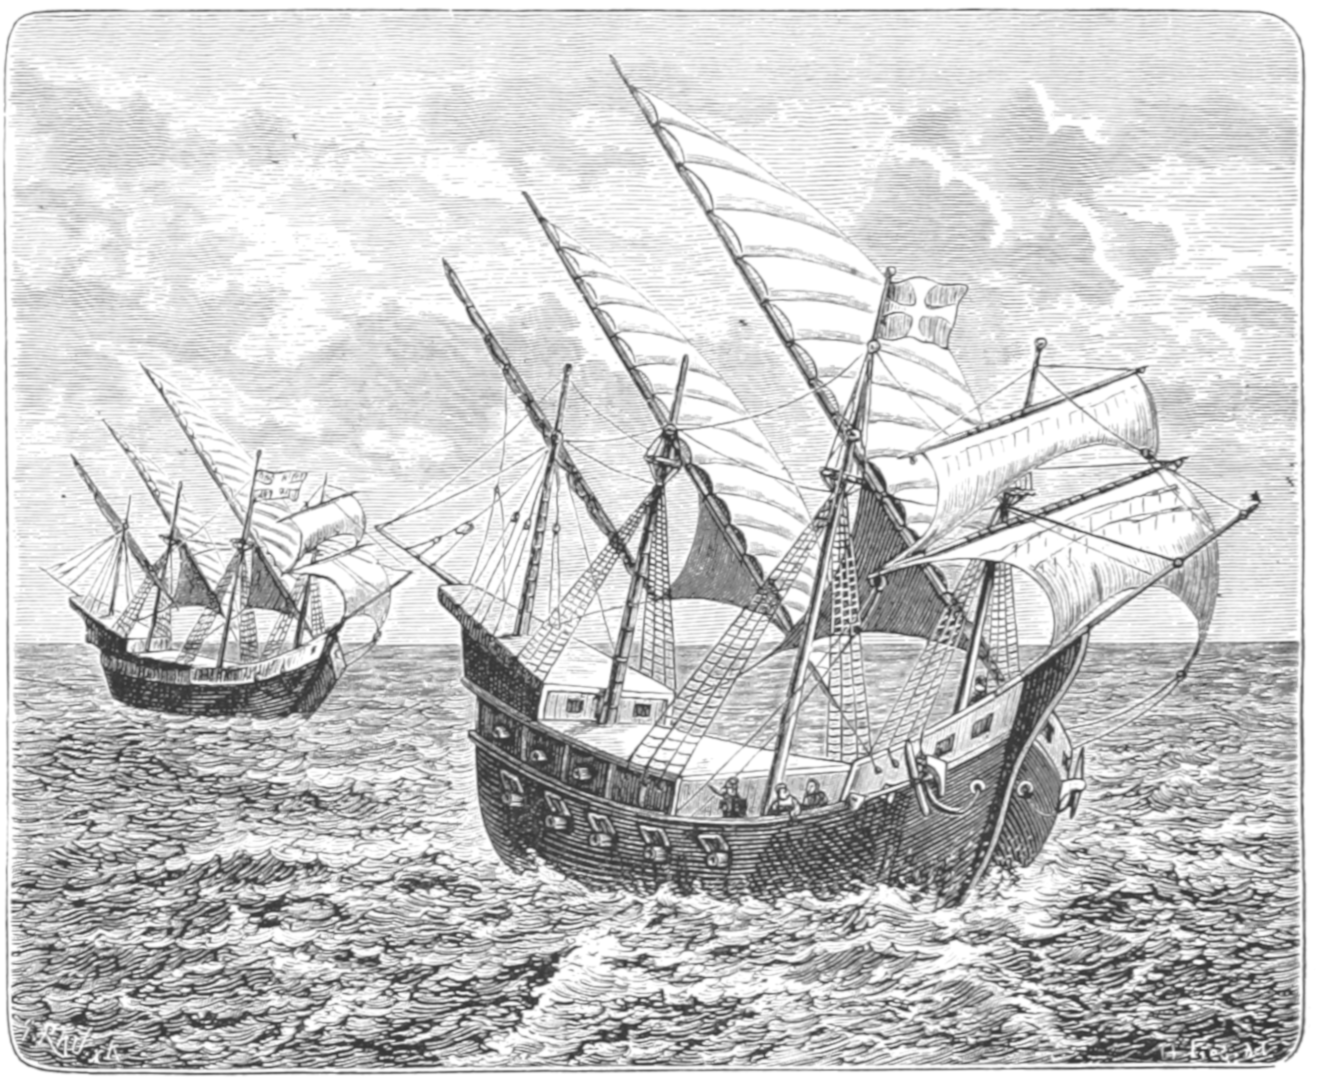
\includegraphics{Fig/Caravelas.png}
{\emph{Bartolomeu dias em sua viagem ao cabo.} \\ Imagem do livro ``The Sea: its stirring story of adventure, peril \& heroism.''; Frederick Whymper; Cassell \& Co., Londres, 1887. \url{https://www.flickr.com/photos/britishlibrary/11288657186/}}
\end{figure*}
\vfill
\begin{fullwidth}
\begin{center}\sc
Elaborado usando \LaTeX \\
documentclass: tufte-book \\
imagens tratadas usando Gimp \\
Figuras elaboradas usando tikz
\end{center}
\end{fullwidth}
\end{document}
